% Options for packages loaded elsewhere
% Options for packages loaded elsewhere
\PassOptionsToPackage{unicode}{hyperref}
\PassOptionsToPackage{hyphens}{url}
\PassOptionsToPackage{dvipsnames,svgnames,x11names}{xcolor}
%
\documentclass[
  letterpaper,
  DIV=11,
  numbers=noendperiod,
  oneside]{scrreprt}
\usepackage{xcolor}
\usepackage[left=1in,marginparwidth=2.0666666666667in,textwidth=4.1333333333333in,marginparsep=0.3in]{geometry}
\usepackage{amsmath,amssymb}
\setcounter{secnumdepth}{4}
\usepackage{iftex}
\ifPDFTeX
  \usepackage[T1]{fontenc}
  \usepackage[utf8]{inputenc}
  \usepackage{textcomp} % provide euro and other symbols
\else % if luatex or xetex
  \usepackage{unicode-math} % this also loads fontspec
  \defaultfontfeatures{Scale=MatchLowercase}
  \defaultfontfeatures[\rmfamily]{Ligatures=TeX,Scale=1}
\fi
\usepackage{lmodern}
\ifPDFTeX\else
  % xetex/luatex font selection
\fi
% Use upquote if available, for straight quotes in verbatim environments
\IfFileExists{upquote.sty}{\usepackage{upquote}}{}
\IfFileExists{microtype.sty}{% use microtype if available
  \usepackage[]{microtype}
  \UseMicrotypeSet[protrusion]{basicmath} % disable protrusion for tt fonts
}{}
\makeatletter
\@ifundefined{KOMAClassName}{% if non-KOMA class
  \IfFileExists{parskip.sty}{%
    \usepackage{parskip}
  }{% else
    \setlength{\parindent}{0pt}
    \setlength{\parskip}{6pt plus 2pt minus 1pt}}
}{% if KOMA class
  \KOMAoptions{parskip=half}}
\makeatother
% Make \paragraph and \subparagraph free-standing
\makeatletter
\ifx\paragraph\undefined\else
  \let\oldparagraph\paragraph
  \renewcommand{\paragraph}{
    \@ifstar
      \xxxParagraphStar
      \xxxParagraphNoStar
  }
  \newcommand{\xxxParagraphStar}[1]{\oldparagraph*{#1}\mbox{}}
  \newcommand{\xxxParagraphNoStar}[1]{\oldparagraph{#1}\mbox{}}
\fi
\ifx\subparagraph\undefined\else
  \let\oldsubparagraph\subparagraph
  \renewcommand{\subparagraph}{
    \@ifstar
      \xxxSubParagraphStar
      \xxxSubParagraphNoStar
  }
  \newcommand{\xxxSubParagraphStar}[1]{\oldsubparagraph*{#1}\mbox{}}
  \newcommand{\xxxSubParagraphNoStar}[1]{\oldsubparagraph{#1}\mbox{}}
\fi
\makeatother

\usepackage{color}
\usepackage{fancyvrb}
\newcommand{\VerbBar}{|}
\newcommand{\VERB}{\Verb[commandchars=\\\{\}]}
\DefineVerbatimEnvironment{Highlighting}{Verbatim}{commandchars=\\\{\}}
% Add ',fontsize=\small' for more characters per line
\usepackage{framed}
\definecolor{shadecolor}{RGB}{241,243,245}
\newenvironment{Shaded}{\begin{snugshade}}{\end{snugshade}}
\newcommand{\AlertTok}[1]{\textcolor[rgb]{0.68,0.00,0.00}{#1}}
\newcommand{\AnnotationTok}[1]{\textcolor[rgb]{0.37,0.37,0.37}{#1}}
\newcommand{\AttributeTok}[1]{\textcolor[rgb]{0.40,0.45,0.13}{#1}}
\newcommand{\BaseNTok}[1]{\textcolor[rgb]{0.68,0.00,0.00}{#1}}
\newcommand{\BuiltInTok}[1]{\textcolor[rgb]{0.00,0.23,0.31}{#1}}
\newcommand{\CharTok}[1]{\textcolor[rgb]{0.13,0.47,0.30}{#1}}
\newcommand{\CommentTok}[1]{\textcolor[rgb]{0.37,0.37,0.37}{#1}}
\newcommand{\CommentVarTok}[1]{\textcolor[rgb]{0.37,0.37,0.37}{\textit{#1}}}
\newcommand{\ConstantTok}[1]{\textcolor[rgb]{0.56,0.35,0.01}{#1}}
\newcommand{\ControlFlowTok}[1]{\textcolor[rgb]{0.00,0.23,0.31}{\textbf{#1}}}
\newcommand{\DataTypeTok}[1]{\textcolor[rgb]{0.68,0.00,0.00}{#1}}
\newcommand{\DecValTok}[1]{\textcolor[rgb]{0.68,0.00,0.00}{#1}}
\newcommand{\DocumentationTok}[1]{\textcolor[rgb]{0.37,0.37,0.37}{\textit{#1}}}
\newcommand{\ErrorTok}[1]{\textcolor[rgb]{0.68,0.00,0.00}{#1}}
\newcommand{\ExtensionTok}[1]{\textcolor[rgb]{0.00,0.23,0.31}{#1}}
\newcommand{\FloatTok}[1]{\textcolor[rgb]{0.68,0.00,0.00}{#1}}
\newcommand{\FunctionTok}[1]{\textcolor[rgb]{0.28,0.35,0.67}{#1}}
\newcommand{\ImportTok}[1]{\textcolor[rgb]{0.00,0.46,0.62}{#1}}
\newcommand{\InformationTok}[1]{\textcolor[rgb]{0.37,0.37,0.37}{#1}}
\newcommand{\KeywordTok}[1]{\textcolor[rgb]{0.00,0.23,0.31}{\textbf{#1}}}
\newcommand{\NormalTok}[1]{\textcolor[rgb]{0.00,0.23,0.31}{#1}}
\newcommand{\OperatorTok}[1]{\textcolor[rgb]{0.37,0.37,0.37}{#1}}
\newcommand{\OtherTok}[1]{\textcolor[rgb]{0.00,0.23,0.31}{#1}}
\newcommand{\PreprocessorTok}[1]{\textcolor[rgb]{0.68,0.00,0.00}{#1}}
\newcommand{\RegionMarkerTok}[1]{\textcolor[rgb]{0.00,0.23,0.31}{#1}}
\newcommand{\SpecialCharTok}[1]{\textcolor[rgb]{0.37,0.37,0.37}{#1}}
\newcommand{\SpecialStringTok}[1]{\textcolor[rgb]{0.13,0.47,0.30}{#1}}
\newcommand{\StringTok}[1]{\textcolor[rgb]{0.13,0.47,0.30}{#1}}
\newcommand{\VariableTok}[1]{\textcolor[rgb]{0.07,0.07,0.07}{#1}}
\newcommand{\VerbatimStringTok}[1]{\textcolor[rgb]{0.13,0.47,0.30}{#1}}
\newcommand{\WarningTok}[1]{\textcolor[rgb]{0.37,0.37,0.37}{\textit{#1}}}

\usepackage{longtable,booktabs,array}
\newcounter{none} % for unnumbered tables
\usepackage{calc} % for calculating minipage widths
% Correct order of tables after \paragraph or \subparagraph
\usepackage{etoolbox}
\makeatletter
\patchcmd\longtable{\par}{\if@noskipsec\mbox{}\fi\par}{}{}
\makeatother
% Allow footnotes in longtable head/foot
\IfFileExists{footnotehyper.sty}{\usepackage{footnotehyper}}{\usepackage{footnote}}
\makesavenoteenv{longtable}
\usepackage{graphicx}
\makeatletter
\newsavebox\pandoc@box
\newcommand*\pandocbounded[1]{% scales image to fit in text height/width
  \sbox\pandoc@box{#1}%
  \Gscale@div\@tempa{\textheight}{\dimexpr\ht\pandoc@box+\dp\pandoc@box\relax}%
  \Gscale@div\@tempb{\linewidth}{\wd\pandoc@box}%
  \ifdim\@tempb\p@<\@tempa\p@\let\@tempa\@tempb\fi% select the smaller of both
  \ifdim\@tempa\p@<\p@\scalebox{\@tempa}{\usebox\pandoc@box}%
  \else\usebox{\pandoc@box}%
  \fi%
}
% Set default figure placement to htbp
\def\fps@figure{htbp}
\makeatother

\ifLuaTeX
  \usepackage{luacolor}
  \usepackage[soul]{lua-ul}
\else
  \usepackage{soul}
\fi

% definitions for citeproc citations
\NewDocumentCommand\citeproctext{}{}
\NewDocumentCommand\citeproc{mm}{%
  \begingroup\def\citeproctext{#2}\cite{#1}\endgroup}
\makeatletter
 % allow citations to break across lines
 \let\@cite@ofmt\@firstofone
 % avoid brackets around text for \cite:
 \def\@biblabel#1{}
 \def\@cite#1#2{{#1\if@tempswa , #2\fi}}
\makeatother
\newlength{\cslhangindent}
\setlength{\cslhangindent}{1.5em}
\newlength{\csllabelwidth}
\setlength{\csllabelwidth}{3em}
\newenvironment{CSLReferences}[2] % #1 hanging-indent, #2 entry-spacing
 {\begin{list}{}{%
  \setlength{\itemindent}{0pt}
  \setlength{\leftmargin}{0pt}
  \setlength{\parsep}{0pt}
  % turn on hanging indent if param 1 is 1
  \ifodd #1
   \setlength{\leftmargin}{\cslhangindent}
   \setlength{\itemindent}{-1\cslhangindent}
  \fi
  % set entry spacing
  \setlength{\itemsep}{#2\baselineskip}}}
 {\end{list}}
\usepackage{calc}
\newcommand{\CSLBlock}[1]{\hfill\break\parbox[t]{\linewidth}{\strut\ignorespaces#1\strut}}
\newcommand{\CSLLeftMargin}[1]{\parbox[t]{\csllabelwidth}{\strut#1\strut}}
\newcommand{\CSLRightInline}[1]{\parbox[t]{\linewidth - \csllabelwidth}{\strut#1\strut}}
\newcommand{\CSLIndent}[1]{\hspace{\cslhangindent}#1}



\setlength{\emergencystretch}{3em} % prevent overfull lines

\providecommand{\tightlist}{%
  \setlength{\itemsep}{0pt}\setlength{\parskip}{0pt}}



 


\KOMAoption{captions}{tableheading}
% ============================================================
% Packages
% ============================================================

\usepackage{physics}
\usepackage{braket}

% ============================================================
% Constants and Basic Symbols
% ============================================================

\newcommand{\me}{{\mathrm e}}

\newcommand{\rss}{\mathrm{RSS}}
\newcommand{\ols}{\mathrm{OLS}}
\newcommand{\ridge}{\mathrm{ridge}}
\newcommand{\lasso}{\mathrm{lasso}}
\newcommand{\mle}{\mathrm{MLE}}
\newcommand{\constant}{\mathrm{constant}}
\newcommand{\resid}{\mathrm{residual}}
% \renewcommand{\span}{\mathrm{span}}
\newcommand{\gini}{\mathrm{Gini}}
\newcommand{\logit}{\operatorname{logit}}

\newcommand{\argmin}{\operatorname*{argmin}}
\newcommand{\argmax}{\operatorname*{argmax}}

% ============================================================
% Probability
% ============================================================

\newcommand{\Exp}{\operatorname{E}}
\newcommand{\Var}{\operatorname{Var}}
\newcommand{\Cov}{\operatorname{Cov}}
\newcommand{\Mode}{\operatorname{mode}}
\newcommand{\cor}{\operatorname{Corr}}

\newcommand{\nll}{\operatorname{nll}}

% ============================================================
% Distribution Names (scipy.stats style)
% ============================================================

\newcommand{\pdfbinom}{{\ttfamily binom}}
\newcommand{\pdfbeta}{{\ttfamily beta}}
\newcommand{\pdfpois}{{\ttfamily poisson}}
\newcommand{\pdfgamma}{{\ttfamily gamma}}
\newcommand{\pdfnormal}{{\ttfamily norm}}
\newcommand{\pdfexp}{{\ttfamily expon}}

% ============================================================
% Probability Distributions
% ============================================================

\newcommand{\distbinom}{\operatorname{B}}
\newcommand{\distbeta}{\operatorname{Beta}}
\newcommand{\distgamma}{\operatorname{Gamma}}
\newcommand{\distexp}{\operatorname{Exp}}
\newcommand{\distpois}{\operatorname{Poisson}}
\newcommand{\distnormal}{\mathcal{N}}

\makeatletter
\@ifpackageloaded{tcolorbox}{}{\usepackage[skins,breakable]{tcolorbox}}
\@ifpackageloaded{fontawesome5}{}{\usepackage{fontawesome5}}
\definecolor{quarto-callout-color}{HTML}{909090}
\definecolor{quarto-callout-note-color}{HTML}{0758E5}
\definecolor{quarto-callout-important-color}{HTML}{CC1914}
\definecolor{quarto-callout-warning-color}{HTML}{EB9113}
\definecolor{quarto-callout-tip-color}{HTML}{00A047}
\definecolor{quarto-callout-caution-color}{HTML}{FC5300}
\definecolor{quarto-callout-color-frame}{HTML}{acacac}
\definecolor{quarto-callout-note-color-frame}{HTML}{4582ec}
\definecolor{quarto-callout-important-color-frame}{HTML}{d9534f}
\definecolor{quarto-callout-warning-color-frame}{HTML}{f0ad4e}
\definecolor{quarto-callout-tip-color-frame}{HTML}{02b875}
\definecolor{quarto-callout-caution-color-frame}{HTML}{fd7e14}
\makeatother
\makeatletter
\@ifpackageloaded{bookmark}{}{\usepackage{bookmark}}
\makeatother
\makeatletter
\@ifpackageloaded{caption}{}{\usepackage{caption}}
\AtBeginDocument{%
\ifdefined\contentsname
  \renewcommand*\contentsname{Table of contents}
\else
  \newcommand\contentsname{Table of contents}
\fi
\ifdefined\listfigurename
  \renewcommand*\listfigurename{List of Figures}
\else
  \newcommand\listfigurename{List of Figures}
\fi
\ifdefined\listtablename
  \renewcommand*\listtablename{List of Tables}
\else
  \newcommand\listtablename{List of Tables}
\fi
\ifdefined\figurename
  \renewcommand*\figurename{Figure}
\else
  \newcommand\figurename{Figure}
\fi
\ifdefined\tablename
  \renewcommand*\tablename{Table}
\else
  \newcommand\tablename{Table}
\fi
}
\@ifpackageloaded{float}{}{\usepackage{float}}
\floatstyle{ruled}
\@ifundefined{c@chapter}{\newfloat{codelisting}{h}{lop}}{\newfloat{codelisting}{h}{lop}[chapter]}
\floatname{codelisting}{Listing}
\newcommand*\listoflistings{\listof{codelisting}{List of Listings}}
\usepackage{amsthm}
\theoremstyle{definition}
\newtheorem{definition}{Definition}[chapter]
\theoremstyle{plain}
\newtheorem{theorem}{Theorem}[chapter]
\theoremstyle{definition}
\newtheorem{example}{Example}[chapter]
\theoremstyle{plain}
\newtheorem{proposition}{Proposition}[chapter]
\theoremstyle{remark}
\AtBeginDocument{\renewcommand*{\proofname}{Proof}}
\newtheorem*{remark}{Remark}
\newtheorem*{solution}{Solution}
\newtheorem{refremark}{Remark}[chapter]
\newtheorem{refsolution}{Solution}[chapter]
\makeatother
\makeatletter
\makeatother
\makeatletter
\@ifpackageloaded{caption}{}{\usepackage{caption}}
\@ifpackageloaded{subcaption}{}{\usepackage{subcaption}}
\makeatother
\makeatletter
\@ifpackageloaded{sidenotes}{}{\usepackage{sidenotes}}
\@ifpackageloaded{marginnote}{}{\usepackage{marginnote}}
\makeatother
\makeatletter
\@ifpackageloaded{tikz}{}{\usepackage{tikz}}
\makeatother
        \newcommand*\circled[1]{\tikz[baseline=(char.base)]{
          \node[shape=circle,draw,inner sep=1pt] (char) {{\scriptsize#1}};}}  
                  
\usepackage{bookmark}
\IfFileExists{xurl.sty}{\usepackage{xurl}}{} % add URL line breaks if available
\urlstyle{same}
\hypersetup{
  pdftitle={Basics of Statistical Learning},
  pdfauthor={Weijia Jia},
  colorlinks=true,
  linkcolor={blue},
  filecolor={Maroon},
  citecolor={Blue},
  urlcolor={Blue},
  pdfcreator={LaTeX via pandoc}}


\title{Basics of Statistical Learning}
\author{Weijia Jia}
\date{2026-07-29}
\begin{document}
\maketitle

\renewcommand*\contentsname{Table of contents}
{
\setcounter{tocdepth}{2}
\tableofcontents
}

\bookmarksetup{startatroot}

\chapter*{Preface}\label{preface}
\addcontentsline{toc}{chapter}{Preface}

\markboth{Preface}{Preface}

These are notes for STAT 432 Summer 2026 at UIUC. If you have any
questions please contact me.

\section*{References}\label{references}
\addcontentsline{toc}{section}{References}

\markright{References}

\protect\phantomsection\label{refs}
\begin{CSLReferences}{0}{1}
\bibitem[\citeproctext]{ref-Bergstra2012}
\CSLLeftMargin{{[}1{]} }%
\CSLRightInline{\textsc{Bergstra}, J. and \textsc{Bengio}, Y. (2012).
\href{http://jmlr.org/papers/v13/bergstra12a.html}{Random search for
hyper-parameter optimization}. \emph{Journal of Machine Learning
Research} \textbf{13} 281--305.}

\bibitem[\citeproctext]{ref-tikhonov1977solutions}
\CSLLeftMargin{{[}2{]} }%
\CSLRightInline{\textsc{Tikhonov}, A. N. and \textsc{Arsenin}, V. Y.
(1977). \emph{Solutions of ill-posed problems}. Winston.}

\bibitem[\citeproctext]{ref-hastie2009elements}
\CSLLeftMargin{{[}3{]} }%
\CSLRightInline{\textsc{Hastie}, T., \textsc{Tibshirani}, R. and
\textsc{Friedman}, J. (2009). \emph{The elements of statistical
learning}. Springer.}

\bibitem[\citeproctext]{ref-Allen1974}
\CSLLeftMargin{{[}4{]} }%
\CSLRightInline{\textsc{Allen}, D. M. (1974).
\href{https://doi.org/10.1080/00401706.1974.10489157}{The relationship
between variable selection and data agumentation and a method for
prediction}. \emph{Technometrics} \textbf{16} 125--7.}

\bibitem[\citeproctext]{ref-verhulst1838}
\CSLLeftMargin{{[}5{]} }%
\CSLRightInline{\textsc{Verhulst}, P.-F. (1838). Notice sur la loi que
la population poursuit dans son accroissement. \emph{Correspondance
Mathématique et Physique} \textbf{10} 113--21.}

\bibitem[\citeproctext]{ref-Berkson1944}
\CSLLeftMargin{{[}6{]} }%
\CSLRightInline{\textsc{Berkson}, J. (1944).
\href{https://doi.org/10.1080/01621459.1944.10500699}{Application of the
logistic function to bio-assay}. \emph{Journal of the American
Statistical Association} \textbf{39} 357--65.}

\bibitem[\citeproctext]{ref-Breiman1984}
\CSLLeftMargin{{[}7{]} }%
\CSLRightInline{\textsc{Breiman}, L., \textsc{Friedman}, J. H.,
\textsc{Olshen}, R. A. and \textsc{Stone}, C. J. (1984).
\emph{\href{https://doi.org/10.1201/9781315139470}{Classification and
regression trees}}. L. Breiman, ed Chapman \& Hall/CRC, Boca Raton, Fla.
{[}u.a.{]}.}

\bibitem[\citeproctext]{ref-breiman2001random}
\CSLLeftMargin{{[}8{]} }%
\CSLRightInline{\textsc{Breiman}, L. (2001). Random forests.
\emph{Machine Learning} \textbf{45} 5--32.}

\bibitem[\citeproctext]{ref-Lin2006}
\CSLLeftMargin{{[}9{]} }%
\CSLRightInline{\textsc{Lin}, Y. and \textsc{Jeon}, Y. (2006).
\href{https://doi.org/10.1198/016214505000001230}{Random forests and
adaptive nearest neighbors}. \emph{Journal of the American Statistical
Association} \textbf{101} 578--90.}

\bibitem[\citeproctext]{ref-Freund1995}
\CSLLeftMargin{{[}10{]} }%
\CSLRightInline{\textsc{Freund}, Y. and \textsc{Schapire}, R. E. (1995).
\href{https://doi.org/10.1007/3-540-59119-2_166}{A desicion-theoretic
generalization of on-line learning and an application to boosting}. In
\emph{Computational learning theory} pp 23--37. Springer Berlin
Heidelberg.}

\bibitem[\citeproctext]{ref-Freund1997}
\CSLLeftMargin{{[}11{]} }%
\CSLRightInline{\textsc{Freund}, Y. and \textsc{Schapire}, R. E. (1997).
\href{https://doi.org/10.1006/jcss.1997.1504}{A decision-theoretic
generalization of on-line learning and an application to boosting}.
\emph{Journal of Computer and System Sciences} \textbf{55} 119--39.}

\bibitem[\citeproctext]{ref-Schapire1998}
\CSLLeftMargin{{[}12{]} }%
\CSLRightInline{\textsc{Schapire}, R. E., \textsc{Freund}, Y.,
\textsc{Bartlett}, P. and \textsc{Lee}, W. S. (1998).
\href{https://doi.org/10.1214/aos/1024691352}{Boosting the margin: A new
explanation for the effectiveness of voting methods}. \emph{The Annals
of Statistics} \textbf{26} 1651--86.}

\bibitem[\citeproctext]{ref-Friedman2000}
\CSLLeftMargin{{[}13{]} }%
\CSLRightInline{\textsc{Friedman}, J., \textsc{Hastie}, T. and
\textsc{Tibshirani}, R. (2000).
\href{https://doi.org/10.1214/aos/1016218223}{Additive logistic
regression: A statistical view of boosting (with discussion and a
rejoinder by the authors)}. \emph{The Annals of Statistics} \textbf{28}
337--407.}

\bibitem[\citeproctext]{ref-Breiman1999}
\CSLLeftMargin{{[}14{]} }%
\CSLRightInline{\textsc{Breiman}, L. (1999).
\href{https://doi.org/10.1162/089976699300016106}{Prediction games and
arcing algorithms}. \emph{Neural Computation} \textbf{11} 1493--517.}

\end{CSLReferences}

\part{Foundations}

\chapter{What is Statistical
Learning?}\label{what-is-statistical-learning}

\section{Introduction}\label{introduction}

Statistical learning studies how to use data to understand relationships
and make predictions.

In supervised learning, a common abstract model is

\[
Y = f(X) + \varepsilon,
\]

where:

\begin{itemize}
\tightlist
\item
  \(X\) represents features;
\item
  \(Y\) represents the response;
\item
  \(f\) is the underlying relationship;
\item
  \(\varepsilon\) represents random noise or unexplained variation.
\end{itemize}

The main objective is to estimate the unknown function \(f\) using
observed data.

More broadly, modern statistical learning is fundamentally about
learning patterns that generalize well to unseen data.

Depending on the objective, statistical learning problems can be viewed
from several different perspectives.

{\def\LTcaptype{none} % do not increment counter
\begin{longtable}[]{@{}ll@{}}
\toprule\noalign{}
Task & Main Question \\
\midrule\noalign{}
\endhead
\bottomrule\noalign{}
\endlastfoot
Prediction & What will happen? \\
Inference & Which variables matter? \\
Causality & What happens if we intervene? \\
\end{longtable}
}

\begin{itemize}
\tightlist
\item
  Prediction mainly focuses on predictive performance and
  generalization. A common formulation is \[
  \hat f(x) \approx \mathbb{E}[Y \mid X=x].
  \]
\item
  Inference focuses on understanding relationships between variables and
  often relies on tools such as confidence intervals and hypothesis
  testing.
\item
  Causality studies intervention effects and is often written as \[
  \mathbb{E}[Y \mid \text{do}(X=x)].
  \]
\end{itemize}

\begin{tcolorbox}[enhanced jigsaw, arc=.35mm, bottomrule=.15mm, bottomtitle=1mm, breakable, colback=white, colbacktitle=quarto-callout-note-color!10!white, colframe=quarto-callout-note-color-frame, coltitle=black, left=2mm, leftrule=.75mm, opacityback=0, opacitybacktitle=0.6, rightrule=.15mm, title=\textcolor{quarto-callout-note-color}{\faInfo}\hspace{0.5em}{Important distinctions}, titlerule=0mm, toprule=.15mm, toptitle=1mm]

\begin{enumerate}
\def\labelenumi{\arabic{enumi}.}
\tightlist
\item
  Good training performance does not imply good generalization.
\item
  Good prediction does not imply valid inference.
\item
  Association does not imply causation.
\end{enumerate}

\end{tcolorbox}

\begin{tcolorbox}[enhanced jigsaw, arc=.35mm, bottomrule=.15mm, bottomtitle=1mm, breakable, colback=white, colbacktitle=quarto-callout-tip-color!10!white, colframe=quarto-callout-tip-color-frame, coltitle=black, left=2mm, leftrule=.75mm, opacityback=0, opacitybacktitle=0.6, rightrule=.15mm, title=\textcolor{quarto-callout-tip-color}{\faLightbulb}\hspace{0.5em}{Tip}, titlerule=0mm, toprule=.15mm, toptitle=1mm]

In this course, we will primarily focus on \textbf{prediction} and
\textbf{generalization} rather than formal statistical inference.

\end{tcolorbox}

\section{Types of Learning}\label{types-of-learning}

Statistical learning problems can be divided into several major
categories depending on the available data and learning objective.

We will mainly focus on supervised learning in this course, with some
topics from unsupervised learning.

\subsection{Supervised Learning}\label{supervised-learning}

In supervised learning, we observe both predictors \(X\) and response
\(Y\).

The goal is to predict or explain the response, such as house price
prediction, spam detection, medical diagnosis, etc..

Supervised learning is usually divided into two major tasks:

\begin{itemize}
\tightlist
\item
  \textbf{regression}, where the response is quantitative;
\item
  \textbf{classification}, where the response is categorical.
\end{itemize}

\begin{example}[]\protect\hypertarget{exm-}{}\label{exm-}

~

\begin{itemize}
\tightlist
\item
  predicting salary is a regression problem;
\item
  predicting whether a tumor is benign or malignant is a classification
  problem.
\end{itemize}

\end{example}

\subsection{Unsupervised Learning}\label{unsupervised-learning}

In unsupervised learning, we observe predictors \(X\) but no response
\(Y\).

The goal is to discover hidden structure in the data, such as
clustering, dimensionality reduction, embedding learning, etc..

\subsection{Reinforcement Learning}\label{reinforcement-learning}

In reinforcement learning, an agent interacts with an environment and
learns through rewards and penalties, such as robotics, game playing,
recommendation systems, etc..

\section{Types of Data}\label{types-of-data}

Machine learning methods are strongly connected to data structure, and
different data types often require different modeling strategies.

This course mainly focuses on \textbf{tabular data}, which is the
classical setting in statistics and applied machine learning.

\subsection{Tabular Data}\label{tabular-data}

Tabular data is one of the most common data formats in statistical
learning. It is typically represented as

\[
X \in \mathbb{R}^{n \times p},
\]

where:

\begin{itemize}
\tightlist
\item
  \(n\) is the number of observations;
\item
  \(p\) is the number of predictors.
\end{itemize}

Example:

{\def\LTcaptype{none} % do not increment counter
\begin{longtable}[]{@{}rrrcc@{}}
\toprule\noalign{}
Age & Income & Balance & Student & Default \\
\midrule\noalign{}
\endhead
\bottomrule\noalign{}
\endlastfoot
23 & 50000 & 1200 & Yes & No \\
45 & 90000 & 3000 & No & Yes \\
\end{longtable}
}

In tabular data:

\begin{itemize}
\tightlist
\item
  rows represent observations;
\item
  columns represent variables or features.
\end{itemize}

For supervised learning, datasets usually contain:

\begin{itemize}
\tightlist
\item
  a feature matrix \(X\);
\item
  a target variable \(y\).
\end{itemize}

For unsupervised learning, we typically observe only the feature matrix
\(X\).

Since this course mainly focuses on tabular data, we will usually treat:

\[
X \in \mathbb{R}^{n \times p},
\qquad
y \in \mathbb{R}^n.
\]

\begin{tcolorbox}[enhanced jigsaw, arc=.35mm, bottomrule=.15mm, bottomtitle=1mm, breakable, colback=white, colbacktitle=quarto-callout-caution-color!10!white, colframe=quarto-callout-caution-color-frame, coltitle=black, left=2mm, leftrule=.75mm, opacityback=0, opacitybacktitle=0.6, rightrule=.15mm, title=\textcolor{quarto-callout-caution-color}{\faFire}\hspace{0.5em}{columns correspond to variables}, titlerule=0mm, toprule=.15mm, toptitle=1mm]

The key feature of tabular data is NOT merely the matrix representation.
More importantly, each column corresponds to a variable with its own
semantic meaning, such as age, income, blood pressure, or transaction
count.

\end{tcolorbox}

\begin{tcolorbox}[enhanced jigsaw, arc=.35mm, bottomrule=.15mm, bottomtitle=1mm, breakable, colback=white, colbacktitle=quarto-callout-tip-color!10!white, colframe=quarto-callout-tip-color-frame, coltitle=black, left=2mm, leftrule=.75mm, opacityback=0, opacitybacktitle=0.6, rightrule=.15mm, title=\textcolor{quarto-callout-tip-color}{\faLightbulb}\hspace{0.5em}{Tip}, titlerule=0mm, toprule=.15mm, toptitle=1mm]

Tabular data is particularly well suited for methods such as linear
models and tree-based models. Therefore, these model families will be
the main focus of this course.

\end{tcolorbox}

\subsection{Other Types of Data}\label{other-types-of-data}

Besides tabular data, many machine learning problems involve other data
formats. We briefly mention several common examples that appear in
modern learning tasks.

\begin{tcolorbox}[enhanced jigsaw, arc=.35mm, bottomrule=.15mm, bottomtitle=1mm, breakable, colback=white, colbacktitle=quarto-callout-note-color!10!white, colframe=quarto-callout-note-color-frame, coltitle=black, left=2mm, leftrule=.75mm, opacityback=0, opacitybacktitle=0.6, rightrule=.15mm, title=\textcolor{quarto-callout-note-color}{\faInfo}\hspace{0.5em}{Image Data}, titlerule=0mm, toprule=.15mm, toptitle=1mm]

Image data contains spatial structure, meaning nearby pixels are highly
related.

Modern image models frequently use:

\begin{itemize}
\tightlist
\item
  convolutional neural networks,
\item
  vision transformers.
\end{itemize}

A central goal is to extract meaningful visual patterns such as edges,
textures, shapes, and objects.

\end{tcolorbox}

\begin{tcolorbox}[enhanced jigsaw, arc=.35mm, bottomrule=.15mm, bottomtitle=1mm, breakable, colback=white, colbacktitle=quarto-callout-note-color!10!white, colframe=quarto-callout-note-color-frame, coltitle=black, left=2mm, leftrule=.75mm, opacityback=0, opacitybacktitle=0.6, rightrule=.15mm, title=\textcolor{quarto-callout-note-color}{\faInfo}\hspace{0.5em}{Text Data}, titlerule=0mm, toprule=.15mm, toptitle=1mm]

Text data contains sequential and contextual structure. Modern NLP is
largely based on transformers and large language models.

\end{tcolorbox}

\begin{tcolorbox}[enhanced jigsaw, arc=.35mm, bottomrule=.15mm, bottomtitle=1mm, breakable, colback=white, colbacktitle=quarto-callout-note-color!10!white, colframe=quarto-callout-note-color-frame, coltitle=black, left=2mm, leftrule=.75mm, opacityback=0, opacitybacktitle=0.6, rightrule=.15mm, title=\textcolor{quarto-callout-note-color}{\faInfo}\hspace{0.5em}{Time Series Data}, titlerule=0mm, toprule=.15mm, toptitle=1mm]

Time series data is ordered over time such as stock prices, weather data
and sensor measurements.

\end{tcolorbox}

\begin{tcolorbox}[enhanced jigsaw, arc=.35mm, bottomrule=.15mm, bottomtitle=1mm, breakable, colback=white, colbacktitle=quarto-callout-note-color!10!white, colframe=quarto-callout-note-color-frame, coltitle=black, left=2mm, leftrule=.75mm, opacityback=0, opacitybacktitle=0.6, rightrule=.15mm, title=\textcolor{quarto-callout-note-color}{\faInfo}\hspace{0.5em}{Graph Data}, titlerule=0mm, toprule=.15mm, toptitle=1mm]

Graph data represents relationships between objects, such as social
networks, citation networks, molecular structures.

Modern graph learning often uses graph neural networks.

\end{tcolorbox}

\section{Generalization and Model
Complexity}\label{generalization-and-model-complexity}

\subsection{Training Error and Test
Error}\label{training-error-and-test-error}

Classical regression focuses heavily on checking model assumptions, such
as independence of errors, constant variance, approximate normality.
These assumptions are especially important for formal inference,
including confidence intervals and hypothesis testing.

In statistical learning, however, the primary goal is often
\textbf{predictive performance} rather than formal inference. As a
result, diagnostic tools still remain useful, but they usually play a
secondary role. Their main purpose is often to detect serious issues
such as strong nonlinearity, influential observations, data quality
problems, severe model misspecification.

The central question becomes: How well does the model predict new
observations?

\begin{definition}[Training Error and Test
Error]\protect\hypertarget{def-training-error}{}\label{def-training-error}

~

\begin{itemize}
\tightlist
\item
  The training error measures how well a model fits the training data.
\item
  The test error measures prediction error on new observations not used
  to fit the model.
\end{itemize}

\end{definition}

For example, suppose we evaluate a regression model using mean squared
error (MSE).

The \textbf{training MSE} measures fit on the observed training sample,
while the \textbf{test MSE} measures prediction performance on new data
drawn from the same population.

A model may achieve extremely small training error while still
performing poorly on unseen data. This happens because the model begins
fitting random noise rather than the underlying signal.

\begin{definition}[Overfitting]\protect\hypertarget{def-overfitting}{}\label{def-overfitting}

Overfitting occurs when a model fits the training data very closely but
fails to generalize well to new data. In this case, the model captures
random noise or idiosyncrasies in the training sample rather than the
underlying relationship.

\end{definition}

Model selection methods attempt to balance model complexity and
prediction accuracy in order to avoid overfitting.

\subsection{Bias--Variance Tradeoff}\label{biasvariance-tradeoff}

A central idea behind generalization is the \textbf{bias--variance
tradeoff}.

Suppose

\[
Y=f(X)+\varepsilon,
\qquad
\Var(\varepsilon)=\sigma^2.
\]

For a fitted estimator \(\hat f\), the test mean squared error at
\(x_0\) satisfies

\[
\Exp\qty[(Y_0-\hat f(x_0))^2]=
\operatorname{Bias}^2(\hat f(x_0))
+
\Var(\hat f(x_0))
+
\sigma^2.
\]

The three terms represent:

\begin{itemize}
\tightlist
\item
  \textbf{bias}: systematic modeling error:
  \(\operatorname{Bias}(\hat f(x))=\Exp[\hat f (x)]-f(x)\). It measures
  the systematic difference between the average prediction and the true
  underlying function;
\item
  \textbf{variance}: sensitivity to the training sample:
  \(\operatorname{Var}(\hat f(x))\). It measures how much the fitted
  model changes when the training data changes. Highly flexible models
  often have larger variance;
\item
  \textbf{irreducible error}: \(\sigma^2\). This represents random noise
  or variability in the data generation process that cannot be explained
  or removed, even with the true model.
\end{itemize}

Roughly speaking, as model flexibility increases:

\begin{itemize}
\tightlist
\item
  training error usually decreases;
\item
  test error often first decreases and then increases.
\end{itemize}

Model selection aims to balance these two effects in order to achieve
good generalization performance.

\begin{tcolorbox}[enhanced jigsaw, arc=.35mm, bottomrule=.15mm, bottomtitle=1mm, breakable, colback=white, colbacktitle=quarto-callout-note-color!10!white, colframe=quarto-callout-note-color-frame, coltitle=black, left=2mm, leftrule=.75mm, opacityback=0, opacitybacktitle=0.6, rightrule=.15mm, title=\textcolor{quarto-callout-note-color}{\faInfo}\hspace{0.5em}{Information Criteria and Estimated Test Error}, titlerule=0mm, toprule=.15mm, toptitle=1mm]

Classical regression often estimates expected test error indirectly
using only the training data.

Some commonly used criteria are:

\begin{itemize}
\tightlist
\item
  AIC (Akaike Information Criterion),
\item
  BIC (Bayesian Information Criterion),
\item
  Mallows' \(C_p\).
\end{itemize}

These criteria reward good fit while penalizing excessive model
complexity.

Although they are useful for model comparison, they still rely on
approximations derived from the training sample.

\end{tcolorbox}

\subsection{Underfit vs Overfit}\label{underfit-vs-overfit}

Bias and variance are closely related to underfit and overfit.

Roughly speaking, underfit means the model is not sufficient to fit the
training samples, and overfit means that the models learns too many
noise from the data. In many cases, high bias is related to underfit,
and high variance is related to overfit.

The following example is from
\href{https://scikit-learn.org/stable/auto_examples/model_selection/plot_underfitting_overfitting.html\#sphx-glr-auto-examples-model-selection-plot-underfitting-overfitting-py}{the
\texttt{sklearn} guide}. Although it is a polynomial regression example,
it grasps the key idea of underfit and overfit.

\begin{figure*}[H]

\pandocbounded{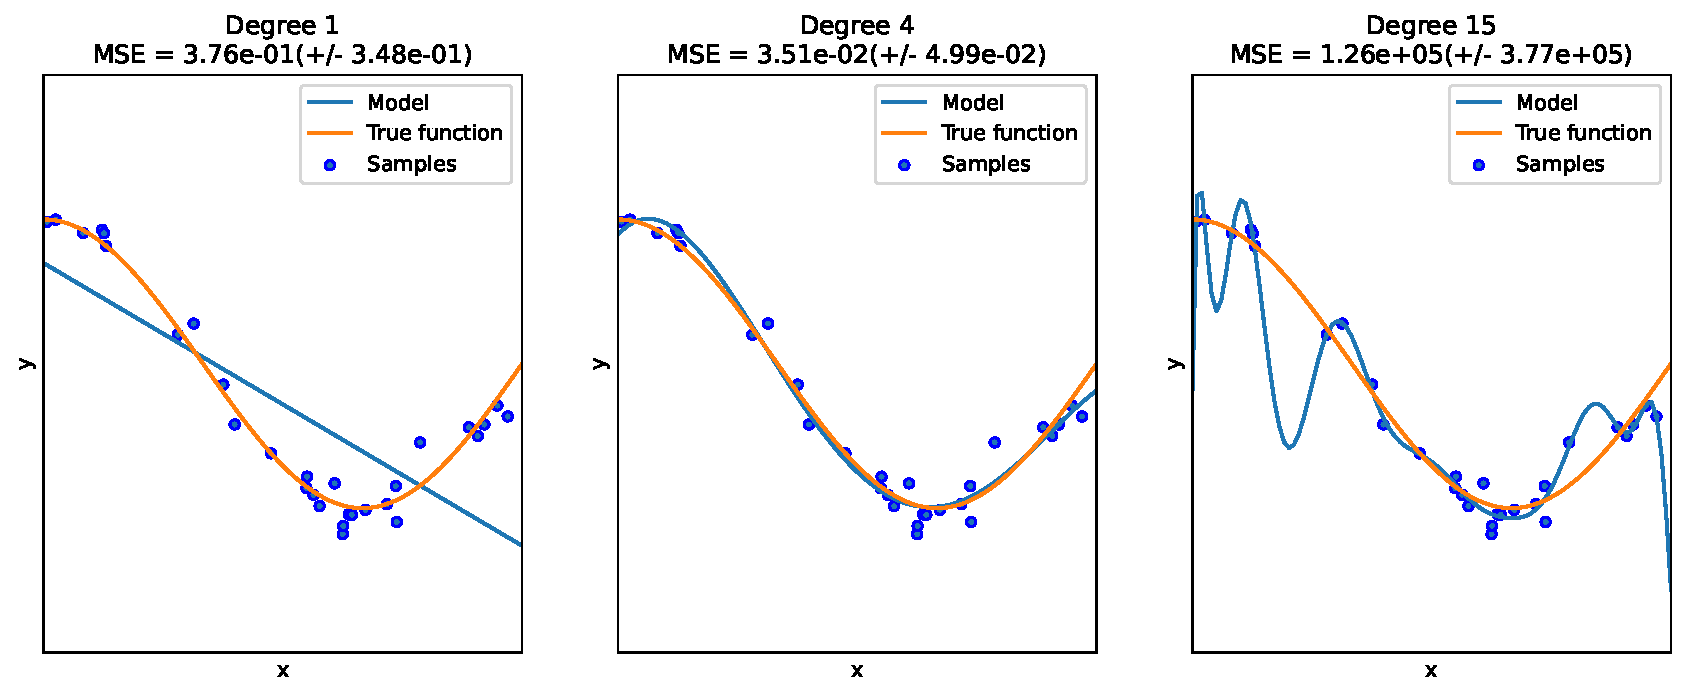
\includegraphics[keepaspectratio]{contents/0/basic_files/figure-pdf/cell-2-output-1.pdf}}

\end{figure*}

\chapter{Classification Decisions and Evaluation}\label{sec-cla_dec}

Unlike regression, where metrics such as Mean Squared Error (MSE)
evaluate prediction error along a continuous scale, classification
evaluation is fundamentally more nuanced.

A modern statistical learning classifier often produces a score or
estimated probability rather than directly outputting a categorical
decision. For example, a model may estimate

\[
\hat p(x)=\Pr(Y=1\mid X=x),
\]

and a separate decision rule then converts this soft prediction into a
hard classification. As a result, classification performance can be
evaluated from several different perspectives.

Broadly speaking, classification evaluation can be divided into three
related but distinct goals.

{\def\LTcaptype{none} % do not increment counter
\begin{longtable}[]{@{}
  >{\raggedright\arraybackslash}p{(\linewidth - 4\tabcolsep) * \real{0.3333}}
  >{\raggedright\arraybackslash}p{(\linewidth - 4\tabcolsep) * \real{0.3333}}
  >{\raggedright\arraybackslash}p{(\linewidth - 4\tabcolsep) * \real{0.3333}}@{}}
\toprule\noalign{}
\begin{minipage}[b]{\linewidth}\raggedright
Goal
\end{minipage} & \begin{minipage}[b]{\linewidth}\raggedright
Main question
\end{minipage} & \begin{minipage}[b]{\linewidth}\raggedright
Common tools
\end{minipage} \\
\midrule\noalign{}
\endhead
\bottomrule\noalign{}
\endlastfoot
Decision quality & Are the final classification decisions good? &
Accuracy, precision, recall, F1-score \\
Ranking quality & Are positive observations ranked above negative
observations? & ROC curve, AUC, PR curve \\
Probability quality & Are predicted probabilities numerically
trustworthy? & Calibration curve, Brier score, log loss \\
\end{longtable}
}

These goals are related but not equivalent. Accurate estimation of
\(\Pr(Y\mid X)\) is the most informative objective because it naturally
supports both ranking and decision-making. In contrast, good performance
on a threshold-based metric such as accuracy does not guarantee
well-calibrated probabilities or reliable rankings.

In practice, however, decision quality is often easier to achieve and is
frequently the primary objective in applied statistical learning. Many
real-world applications ultimately require concrete actions, such as
approving a loan, detecting fraud, or diagnosing disease. Consequently,
threshold-based metrics such as accuracy, precision, recall, and
F1-score often play the central role in applied machine learning.

\begin{tcolorbox}[enhanced jigsaw, arc=.35mm, bottomrule=.15mm, bottomtitle=1mm, breakable, colback=white, colbacktitle=quarto-callout-note-color!10!white, colframe=quarto-callout-note-color-frame, coltitle=black, left=2mm, leftrule=.75mm, opacityback=0, opacitybacktitle=0.6, rightrule=.15mm, title=\textcolor{quarto-callout-note-color}{\faInfo}\hspace{0.5em}{Note}, titlerule=0mm, toprule=.15mm, toptitle=1mm]

Classification evaluation can become quite sophisticated and may involve
ranking performance, probability calibration, cost-sensitive learning,
threshold optimization, and decision theory.

In this course, however, our primary goal is to understand the core
ideas of statistical learning and predictive modeling rather than to
develop a complete theory of statistical decision making. Therefore, we
will mainly focus on accuracy and closely related threshold-based
classification metrics.

\end{tcolorbox}

\section{Decision quality}\label{decision-quality}

Decision quality evaluates the final hard classifications after applying
a threshold to predicted scores or probabilities.

This perspective focuses on whether the model makes useful decisions in
practice. Metrics such as accuracy, precision, recall, and F1-score
belong to this category.

\subsection{Binary Classification
Setup}\label{binary-classification-setup}

Suppose the response is binary:

\[
Y\in\{0,1\}.
\]

We call \(Y=1\) the positive class and \(Y=0\) the negative class.

A classifier produces a predicted label

\[
\hat Y\in\{0,1\}.
\]

The four possible outcomes are summarized by the confusion matrix.

{\def\LTcaptype{none} % do not increment counter
\begin{longtable}[]{@{}lrr@{}}
\toprule\noalign{}
& Predicted positive & Predicted negative \\
\midrule\noalign{}
\endhead
\bottomrule\noalign{}
\endlastfoot
True positive class & TP & FN \\
True negative class & FP & TN \\
\end{longtable}
}

Here, TP means true positive, FP means false positive, FN means false
negative, TN means true negative.

The confusion matrix is the starting point for most threshold-based
classification metrics.

\subsection{Accuracy}\label{accuracy}

Accuracy is the proportion of correctly classified observations:

\[
\text{Accuracy}
=
\frac{TP+TN}{TP+FP+FN+TN}.
\]

Accuracy is simple and useful when:

\begin{itemize}
\tightlist
\item
  the classes are reasonably balanced,
\item
  false positives and false negatives have similar costs,
\item
  the decision threshold is already fixed and meaningful.
\end{itemize}

However, accuracy can be misleading.

Suppose only \(1\%\) of observations are positive. A classifier that
always predicts negative has \(99\%\) accuracy, but it never detects a
positive case. In many applications, that classifier is useless.

\begin{tcolorbox}[enhanced jigsaw, arc=.35mm, bottomrule=.15mm, bottomtitle=1mm, breakable, colback=white, colbacktitle=quarto-callout-caution-color!10!white, colframe=quarto-callout-caution-color-frame, coltitle=black, left=2mm, leftrule=.75mm, opacityback=0, opacitybacktitle=0.6, rightrule=.15mm, title=\textcolor{quarto-callout-caution-color}{\faFire}\hspace{0.5em}{Accuracy is not enough}, titlerule=0mm, toprule=.15mm, toptitle=1mm]

Accuracy implicitly treats all mistakes as equally costly.

When classes are imbalanced or error costs are asymmetric, accuracy can
hide the most important behavior of the classifier.

\end{tcolorbox}

\subsection{Recall (sensitivity)}\label{recall-sensitivity}

Recall is defined as

\[
\text{Recall}
=
\frac{TP}{TP+FN}.
\]

Recall answers the question:

\begin{quote}
Among all truly positive observations, how many did we detect?
\end{quote}

In probability notation,

\[
\text{Recall}
=
P(\hat Y=1\mid Y=1).
\]

Recall is also called sensitivity, or true positive rate (TPR).

High recall means few false negatives. Low recall means many true
positive cases were missed.

\begin{tcolorbox}[enhanced jigsaw, arc=.35mm, bottomrule=.15mm, bottomtitle=1mm, breakable, colback=white, colbacktitle=quarto-callout-note-color!10!white, colframe=quarto-callout-note-color-frame, coltitle=black, left=2mm, leftrule=.75mm, opacityback=0, opacitybacktitle=0.6, rightrule=.15mm, title=\textcolor{quarto-callout-note-color}{\faInfo}\hspace{0.5em}{Recall and Statistical Power}, titlerule=0mm, toprule=.15mm, toptitle=1mm]

Recall has a direct connection to hypothesis testing.

Suppose we think of the classification problem as testing

\[
H_0:Y=0
\quad\text{versus}\quad
H_1:Y=1.
\]

Predicting positive is like rejecting \(H_0\). Predicting negative is
like failing to reject \(H_0\).

Under this interpretation:

\begin{itemize}
\tightlist
\item
  a false positive is a Type I error,
\item
  a false negative is a Type II error,
\item
  recall plays a role analogous to statistical power.
\end{itemize}

Thus

\[
\text{Recall}
=
1-\text{Type II error rate}.
\]

Recall measures the ability to detect true signals.

\end{tcolorbox}

\subsection{Precision}\label{precision}

Precision is defined as

\[
\text{Precision}
=
\frac{TP}{TP+FP}.
\]

Precision answers the question:

\begin{quote}
Among all observations predicted positive, how many are truly positive?
\end{quote}

In probability notation,

\[
\text{Precision}
=
P(Y=1\mid \hat Y=1).
\]

Precision is also called positive predictive value.

High precision means positive predictions are trustworthy. Low precision
means many predicted positives are false alarms.

\begin{tcolorbox}[enhanced jigsaw, arc=.35mm, bottomrule=.15mm, bottomtitle=1mm, breakable, colback=white, colbacktitle=quarto-callout-note-color!10!white, colframe=quarto-callout-note-color-frame, coltitle=black, left=2mm, leftrule=.75mm, opacityback=0, opacitybacktitle=0.6, rightrule=.15mm, title=\textcolor{quarto-callout-note-color}{\faInfo}\hspace{0.5em}{Precision vs Recall}, titlerule=0mm, toprule=.15mm, toptitle=1mm]

Precision and recall condition on different events.

Recall conditions on the truth:

\[
P(\hat Y=1\mid Y=1).
\]

Precision conditions on the prediction:

\[
P(Y=1\mid \hat Y=1).
\]

This distinction is very important.

Recall asks whether we find the positives. Precision asks whether our
positive discoveries are reliable. Precision depends strongly on class
prevalence.

\end{tcolorbox}

\subsection{F1 Score}\label{f1-score}

The F1 score combines precision and recall:

\[
F_1
=
\frac{2PR}{P+R},
\]

where \(P\) is precision and \(R\) is recall.

Equivalently,

\[
F_1
=
\frac{2TP}{2TP+FP+FN}.
\]

The F1 score is the harmonic mean of precision and recall.

The harmonic mean strongly penalizes imbalance. If precision is high but
recall is near zero, then F1 is near zero. If recall is high but
precision is near zero, then F1 is also near zero.

F1 is useful when we want a single number that balances precision and
recall. However, it assumes precision and recall are equally important.
In applications where one type of error is more costly, a different
metric or an explicit cost function may be better.

\begin{tcolorbox}[enhanced jigsaw, arc=.35mm, bottomrule=.15mm, bottomtitle=1mm, breakable, colback=white, colbacktitle=quarto-callout-note-color!10!white, colframe=quarto-callout-note-color-frame, coltitle=black, left=2mm, leftrule=.75mm, opacityback=0, opacitybacktitle=0.6, rightrule=.15mm, title=\textcolor{quarto-callout-note-color}{\faInfo}\hspace{0.5em}{Note}, titlerule=0mm, toprule=.15mm, toptitle=1mm]

F1 ignores true negatives entirely.

This can be useful for rare event detection, where the number of true
negatives may dominate the dataset and make accuracy misleading.

\end{tcolorbox}

\subsection{Recall vs Precision}\label{recall-vs-precision}

\subsubsection{Bayes' Rule and Class
Imbalance}\label{bayes-rule-and-class-imbalance}

Precision and recall are connected by Bayes' rule.

Let \(\pi=P(Y=1)\) be the prevalence of the positive class.

\begin{proposition}[]\protect\hypertarget{prp-}{}\label{prp-}

\[
\text{Precision}
=
P(Y=1\mid \hat Y=1)
=
\frac{TPR\cdot\pi}
{TPR\cdot\pi+FPR(1-\pi)}.
\]

This formula shows why precision can be low for rare events: when
\(\pi\) is small, even a modest false positive rate can create many
false positives.

Click to expand.

Let

\[
TPR=P(\hat Y=1\mid Y=1)=\text{Recall}
\]

and

\[
FPR=P(\hat Y=1\mid Y=0).
\]

Then by Bayes' Rule,

\[
\begin{split}
\text{Precision}
=&
P(Y=1\mid \hat Y=1)\\
=&\frac{P(\hat Y=1\mid Y=1)P(Y=1)}{P(\hat Y=1\mid Y=1)P(Y=1)+P(\hat Y=1\mid Y=0)P(Y=0)}\\
=&
\frac{TPR\cdot \pi}
{TPR\cdot \pi+FPR\cdot(1-\pi)}.
\end{split}
\]

\end{proposition}

\begin{example}[Rare Event
Example]\protect\hypertarget{exm-}{}\label{exm-}

~

Click to expand.

Suppose there are 10,000 observations:

\begin{itemize}
\tightlist
\item
  100 positives,
\item
  9,900 negatives.
\end{itemize}

Assume the classifier has:

\[
TPR=0.90,
\quad
FPR=0.05.
\]

Then:

\[
TP=90,
\quad
FP=495.
\]

The recall is high:

\[
\text{Recall}
=
0.90.
\]

But precision is only

\[
\text{Precision}
=
\frac{90}{90+495}
\approx
0.154.
\]

Most predicted positives are false positives. This is why
precision-recall analysis is especially important for imbalanced data.

\end{example}

\subsubsection{Classification
Thresholds}\label{classification-thresholds}

Many classifiers first produce a score or estimated probability:

\[
\hat p(x)=P(Y=1\mid X=x).
\]

To make a hard classification, we choose a threshold \(c\):

\[
\hat Y
=
\begin{cases}
1, & \hat p(x)>c,\\
0, & \hat p(x)\le c.
\end{cases}
\]

The default decision threshold is often \(c=0.5\), but this is not
always the optimal choice. Changing the threshold changes the confusion
matrix, and therefore also changes metrics such as accuracy, precision,
recall, false positive rate (FPR), and F1 score.

To better understand the precision--recall tradeoff, let us examine how
altering the decision threshold changes the behavior of a classifier.

{\def\LTcaptype{none} % do not increment counter
\begin{longtable}[]{@{}
  >{\raggedright\arraybackslash}p{(\linewidth - 14\tabcolsep) * \real{0.1250}}
  >{\raggedright\arraybackslash}p{(\linewidth - 14\tabcolsep) * \real{0.1250}}
  >{\raggedright\arraybackslash}p{(\linewidth - 14\tabcolsep) * \real{0.1250}}
  >{\raggedright\arraybackslash}p{(\linewidth - 14\tabcolsep) * \real{0.1250}}
  >{\raggedright\arraybackslash}p{(\linewidth - 14\tabcolsep) * \real{0.1250}}
  >{\raggedright\arraybackslash}p{(\linewidth - 14\tabcolsep) * \real{0.1250}}
  >{\raggedright\arraybackslash}p{(\linewidth - 14\tabcolsep) * \real{0.1250}}
  >{\raggedright\arraybackslash}p{(\linewidth - 14\tabcolsep) * \real{0.1250}}@{}}
\toprule\noalign{}
\begin{minipage}[b]{\linewidth}\raggedright
Decision Threshold
\end{minipage} & \begin{minipage}[b]{\linewidth}\raggedright
TP
\end{minipage} & \begin{minipage}[b]{\linewidth}\raggedright
TN
\end{minipage} & \begin{minipage}[b]{\linewidth}\raggedright
FP
\end{minipage} & \begin{minipage}[b]{\linewidth}\raggedright
FN
\end{minipage} & \begin{minipage}[b]{\linewidth}\raggedright
Recall
\end{minipage} & \begin{minipage}[b]{\linewidth}\raggedright
Precision
\end{minipage} & \begin{minipage}[b]{\linewidth}\raggedright
Classifier Behavior
\end{minipage} \\
\midrule\noalign{}
\endhead
\bottomrule\noalign{}
\endlastfoot
Lower threshold & Non-decreasing & Non-increasing & Non-decreasing &
Non-increasing & Non-decreasing & May decrease & \\
Higher threshold & Non-increasing & Non-decreasing & Non-increasing &
Non-decreasing & Non-increasing & May increase & \\
\end{longtable}
}

Lowering the threshold classifies more observations as positive.
Therefore, both true positives (TP) and false positives (FP) may
increase, while false negatives (FN) decrease.

Raising the threshold classifies more observations as negative.
Therefore, both true negatives (TN) and false negatives (FN) may
increase, while true positives (TP) decrease.

\begin{example}[Example: Precision Is Not Strictly
Monotone]\protect\hypertarget{exm-}{}\label{exm-}

~

Click to expand.

Consider a small validation dataset with five observations. The model
outputs predicted probabilities \(\hat P(Y=1 \mid X)\), ordered from
highest to lowest.

{\def\LTcaptype{none} % do not increment counter
\begin{longtable}[]{@{}crc@{}}
\toprule\noalign{}
Instance & Predicted Probability & True Label \\
\midrule\noalign{}
\endhead
\bottomrule\noalign{}
\endlastfoot
A & 0.95 & 1 \\
B & 0.90 & 0 \\
C & 0.85 & 1 \\
D & 0.80 & 1 \\
E & 0.70 & 0 \\
\end{longtable}
}

As the threshold is raised, fewer observations are classified as
positive.

{\def\LTcaptype{none} % do not increment counter
\begin{longtable}[]{@{}rlrrr@{}}
\toprule\noalign{}
Threshold & Predicted Positives & TP & FP & Precision \\
\midrule\noalign{}
\endhead
\bottomrule\noalign{}
\endlastfoot
0.75 & A, B, C, D & 3 & 1 & \(3/4 = 0.75\) \\
0.82 & A, B, C & 2 & 1 & \(2/3 \approx 0.67\) \\
0.88 & A, B & 1 & 1 & \(1/2 = 0.50\) \\
0.92 & A & 1 & 0 & \(1/1 = 1.00\) \\
\end{longtable}
}

In this example, raising the threshold first decreases precision because
some true positives are removed while the false positive remains.
Precision increases only after the false positive is also removed.

This shows that precision can move up or down as the threshold changes,
depending on the labels of the observations crossing the threshold.

\end{example}

\begin{tcolorbox}[enhanced jigsaw, arc=.35mm, bottomrule=.15mm, bottomtitle=1mm, breakable, colback=white, colbacktitle=quarto-callout-note-color!10!white, colframe=quarto-callout-note-color-frame, coltitle=black, left=2mm, leftrule=.75mm, opacityback=0, opacitybacktitle=0.6, rightrule=.15mm, title=\textcolor{quarto-callout-note-color}{\faInfo}\hspace{0.5em}{Thresholds are decisions}, titlerule=0mm, toprule=.15mm, toptitle=1mm]

\begin{itemize}
\tightlist
\item
  The fitted model may estimate probabilities.
\item
  The threshold determines the action.
\end{itemize}

Model fitting and decision making are related, but they are not the same
thing.

\end{tcolorbox}

\subsubsection{Decision Theory and Error
Costs}\label{decision-theory-and-error-costs}

Suppose a false positive has cost \(C_{FP}\) and a false negative has
cost \(C_{FN}\).

If a model estimates

\[
p(x)=P(Y=1\mid X=x),
\]

then the expected cost of predicting positive is

\[
\text{Cost}(1\mid x)
=
C_{FP}P(Y=0\mid X=x)
=
C_{FP}(1-p(x)).
\]

The expected cost of predicting negative is

\[
\text{Cost}(0\mid x)
=
C_{FN}P(Y=1\mid X=x)
=
C_{FN}p(x).
\]

We should predict positive when

\[
C_{FP}(1-p(x))
<
C_{FN}p(x).
\]

Solving this inequality gives

\[
p(x)
>
\frac{C_{FP}}{C_{FP}+C_{FN}}.
\]

Thus the optimal threshold is

\[
c^*
=
\frac{C_{FP}}{C_{FP}+C_{FN}}.
\]

This threshold minimizes the expected classification cost under the
assumed probability model.

If false negatives are very costly, then \(C_{FN}\) becomes large, which
lowers the threshold. In this case, the classifier predicts the positive
class more aggressively in order to reduce missed detections.

\begin{example}[Medical
Screening]\protect\hypertarget{exm-}{}\label{exm-}

In medical screening, missing a serious disease may be much worse than
sending a healthy patient for an additional test. Therefore false
negatives are costly.

The threshold should often be lower, so the classifier prioritizes
recall.

\end{example}

\begin{example}[Spam Filtering]\protect\hypertarget{exm-}{}\label{exm-}

In spam filtering, putting an important legitimate email into spam may
be very costly to the user. Therefore false positives may be more
costly.

The threshold should often be higher, so the classifier prioritizes
precision.

\end{example}

\section{Ranking quality}\label{ranking-quality}

Ranking quality evaluates whether positive observations tend to receive
higher scores than negative observations.

This perspective is important when the classification threshold is not
fixed or when the main goal is prioritization rather than direct
classification. ROC curves, AUC, and precision--recall curves are
commonly used to evaluate ranking performance.

\subsection{ROC}\label{roc}

ROC stands for receiver operating characteristic. An ROC curve plots: \[
TPR
=
\frac{TP}{TP+FN}
\quad\text{ against }\quad
FPR
=
\frac{FP}{FP+TN}
\] as the probability threshold varies from 0 to 1.

\subsection{ROC and Hypothesis
Testing}\label{roc-and-hypothesis-testing}

ROC curves have a natural hypothesis testing interpretation. As
discussed before,

\begin{itemize}
\tightlist
\item
  TPR is power,
\item
  FPR is Type I error rate.
\end{itemize}

Therefore an ROC curve shows

\[
\text{power}
\quad\text{versus}\quad
\text{Type I error rate}
\]

across all possible thresholds.

The ideal classifier reaches the upper-left corner:

\[
FPR=0,
\quad
TPR=1.
\]

A classifier close to the diagonal line behaves almost like random
guessing.

\subsection{AUC}\label{auc}

AUC refers to the Area Under the ROC Curve. It summarizes ranking
performance across all possible classification thresholds.

Let \(s(X^+)\) be the score for a randomly selected positive
observation, and let \(s(X^-)\) be the score for a randomly selected
negative observation. Then

\[
AUC
=
P\left(s(X^+)>s(X^-)\right),
\]

up to small corrections for ties.

Thus AUC has a clean probabilistic interpretation:

\begin{quote}
AUC is the probability that a randomly selected positive observation
receives a higher score than a randomly selected negative observation.
\end{quote}

This explains why AUC is threshold-free. It evaluates ranking quality
rather than the quality of a particular classification decision.

Importantly, AUC evaluates relative ordering rather than absolute
probability accuracy.

\begin{tcolorbox}[enhanced jigsaw, arc=.35mm, bottomrule=.15mm, bottomtitle=1mm, breakable, colback=white, colbacktitle=quarto-callout-caution-color!10!white, colframe=quarto-callout-caution-color-frame, coltitle=black, left=2mm, leftrule=.75mm, opacityback=0, opacitybacktitle=0.6, rightrule=.15mm, title=\textcolor{quarto-callout-caution-color}{\faFire}\hspace{0.5em}{AUC is not calibration}, titlerule=0mm, toprule=.15mm, toptitle=1mm]

AUC can be excellent even when predicted probabilities are numerically
inaccurate.

AUC only asks whether positive observations tend to receive higher
scores than negative observations. It does not ask whether the predicted
probabilities themselves are trustworthy or well calibrated.

\end{tcolorbox}

\subsection{Precision-Recall Curve}\label{precision-recall-curve}

A precision-recall curve plots precision against recall as the
classification threshold changes.

It is especially useful when the positive class is rare. In imbalanced
datasets, an ROC curve may look strong because the false positive rate
is divided by the large number of true negatives. However, precision
directly measures how many predicted positives are actually positive.

Average precision summarizes the precision-recall curve as a single
number. Like AUC, it evaluates ranking behavior across thresholds, but
it focuses more directly on performance for the positive class.

\section{Probability Quality}\label{probability-quality}

Probability quality asks whether predicted probabilities can be
interpreted as actual probabilities.

For example, suppose a model predicts \(\hat p(x)=0.8\). If the model is
well calibrated, then among many observations with predicted probability
near \(0.8\), roughly \(80\%\) should truly belong to the positive
class.

Thus probability quality concerns whether predicted probabilities are
numerically trustworthy.

Unlike decision quality or ranking quality, probability quality focuses
on the accuracy of the probability estimates themselves. Calibration
curves, Brier score, and log loss are commonly used to evaluate
probability quality.

\begin{tcolorbox}[enhanced jigsaw, arc=.35mm, bottomrule=.15mm, bottomtitle=1mm, breakable, colback=white, colbacktitle=quarto-callout-note-color!10!white, colframe=quarto-callout-note-color-frame, coltitle=black, left=2mm, leftrule=.75mm, opacityback=0, opacitybacktitle=0.6, rightrule=.15mm, title=\textcolor{quarto-callout-note-color}{\faInfo}\hspace{0.5em}{Note}, titlerule=0mm, toprule=.15mm, toptitle=1mm]

In many practical machine learning applications, probability quality is
less important than classification accuracy or ranking performance.

Therefore, in this course, we will mainly focus on threshold-based
classification metrics such as accuracy, precision, recall, and F1
score. This section is included primarily to provide a broader view of
classification evaluation.

\end{tcolorbox}

\subsection{Calibration Curve}\label{calibration-curve}

A calibration curve, also called a reliability diagram, is constructed
as follows:

\begin{enumerate}
\def\labelenumi{\arabic{enumi}.}
\tightlist
\item
  Divide observations into bins according to predicted probability.
\item
  For each bin, compute the average predicted probability.
\item
  Compute the observed positive proportion in each bin.
\item
  Plot observed proportion against average predicted probability.
\end{enumerate}

For a perfectly calibrated model, the curve follows the diagonal line.

\begin{itemize}
\tightlist
\item
  If the curve lies below the diagonal, the model is overconfident.
\item
  If the curve lies above the diagonal, the model is underconfident.
\end{itemize}

\section{Model Tuning versus Threshold
Tuning}\label{model-tuning-versus-threshold-tuning}

In classification, model fitting and decision making should be viewed as
separate problems.

First, the model estimates a score or probability:

\[
\hat p(x) \approx \Pr(Y=1\mid X=x).
\]

Second, we choose a threshold to convert this probability into an
action.

Model tuning affects the quality of \(\hat p(x)\) itself. This is where
ideas such as bias, variance, regularization, and model complexity
matter. A very flexible classifier may capture nonlinear structure, but
its probability estimates may be unstable or poorly calibrated.

Threshold tuning does not change \(\hat p(x)\). It only changes the
decision rule built on top of the fitted probabilities. Lower thresholds
usually increase recall and false positives; higher thresholds usually
increase precision and reduce false positives.

Thus:

\begin{itemize}
\tightlist
\item
  model tuning controls the fitted scores or probabilities;
\item
  threshold tuning controls the action taken from those scores;
\item
  calibration checks whether the probabilities are numerically
  trustworthy.
\end{itemize}

A good classifier therefore involves not only learning accurate scores,
but also choosing appropriate decision rules for the application.

\section{Python Example: Breast Cancer
Classification}\label{python-example-breast-cancer-classification}

We now use the
\href{https://scikit-learn.org/stable/modules/generated/sklearn.datasets.load_breast_cancer.html}{breast
cancer dataset from \texttt{sklearn}}. The goal is to classify tumors as
malignant or benign. This example shows how to compute threshold-based
metrics, ROC and PR curves, and calibration curves.

In this example, please mainly focus on the evaluation metrics. Other
part like modeling, splitting, etc. will be introduced in later
sections.

\subsection{Load the dataset}\label{load-the-dataset}

First load the data and split it into training and test sets. By
default, the dataset uses \texttt{0} for malignant and \texttt{1} for
benign. Since many classification metrics interpret label \texttt{1} as
the positive class, we redefine malignant as \texttt{1}. Therefore we
need to modify the \texttt{y} value.

\begin{Shaded}
\begin{Highlighting}[]
\ImportTok{from}\NormalTok{ sklearn.datasets }\ImportTok{import}\NormalTok{ load\_breast\_cancer}
\ImportTok{from}\NormalTok{ sklearn.model\_selection }\ImportTok{import}\NormalTok{ train\_test\_split}

\NormalTok{cancer }\OperatorTok{=}\NormalTok{ load\_breast\_cancer(as\_frame}\OperatorTok{=}\VariableTok{True}\NormalTok{)}

\NormalTok{X }\OperatorTok{=}\NormalTok{ cancer.data}
\NormalTok{y\_original }\OperatorTok{=}\NormalTok{ cancer.target}
\NormalTok{y }\OperatorTok{=} \DecValTok{1} \OperatorTok{{-}}\NormalTok{ y\_original}

\NormalTok{X\_train, X\_test, y\_train, y\_test }\OperatorTok{=}\NormalTok{ train\_test\_split(}
\NormalTok{    X, y, test\_size}\OperatorTok{=}\FloatTok{0.3}\NormalTok{, stratify}\OperatorTok{=}\NormalTok{y, random\_state}\OperatorTok{=}\DecValTok{1}
\NormalTok{)}
\end{Highlighting}
\end{Shaded}

We may want to see the distribution of the test set.

\begin{Shaded}
\begin{Highlighting}[]
\ImportTok{import}\NormalTok{ pandas }\ImportTok{as}\NormalTok{ pd}
\NormalTok{pd.Series(y\_test).value\_counts().sort\_index()}
\end{Highlighting}
\end{Shaded}

\begin{verbatim}
target
0    107
1     64
Name: count, dtype: int64
\end{verbatim}

\subsection{Fit models}\label{fit-models}

We fit logistic regression model as an example, which is a typical
strong baseline model.

\begin{Shaded}
\begin{Highlighting}[]
\ImportTok{from}\NormalTok{ sklearn.pipeline }\ImportTok{import}\NormalTok{ make\_pipeline}
\ImportTok{from}\NormalTok{ sklearn.preprocessing }\ImportTok{import}\NormalTok{ StandardScaler}
\ImportTok{from}\NormalTok{ sklearn.linear\_model }\ImportTok{import}\NormalTok{ LogisticRegression}

\NormalTok{logit }\OperatorTok{=}\NormalTok{ make\_pipeline(}
\NormalTok{    StandardScaler(),}
\NormalTok{    LogisticRegression(max\_iter}\OperatorTok{=}\DecValTok{5000}\NormalTok{),}
\NormalTok{)}

\NormalTok{logit.fit(X\_train, y\_train)}

\NormalTok{logit\_prob }\OperatorTok{=}\NormalTok{ logit.predict\_proba(X\_test)[:, }\DecValTok{1}\NormalTok{]}
\end{Highlighting}
\end{Shaded}

Note that \texttt{logit.predict\_proba(X\_test)} returns 2 columns:

\begin{itemize}
\tightlist
\item
  column 0: \(\Pr(Y=0\mid X)\),
\item
  column 1: \(\Pr(Y=1\mid X)\).
\end{itemize}

Since we want the predicted probability for the positive class
(\texttt{y=1}), we select the second column.

\subsection{Confusion Matrix and Basic
Metrics}\label{confusion-matrix-and-basic-metrics}

All decision quality metrics can be computed using functions from
\texttt{sklearn.metrics}. They are used to compare two list-like
objects, while the true labels are passed first and the predicted labels
second.

By default, \texttt{predict()} in \texttt{sklearn} uses threshold
\(0.5\) for binary classification.

\begin{Shaded}
\begin{Highlighting}[]
\ImportTok{from}\NormalTok{ sklearn.metrics }\ImportTok{import}\NormalTok{ accuracy\_score, precision\_score, recall\_score, f1\_score}

\NormalTok{y\_pred }\OperatorTok{=}\NormalTok{ logit.predict(X\_test)}

\NormalTok{acc }\OperatorTok{=}\NormalTok{ accuracy\_score(y\_test, y\_pred)}
\NormalTok{prec }\OperatorTok{=}\NormalTok{ precision\_score(y\_test, y\_pred)}
\NormalTok{rec }\OperatorTok{=}\NormalTok{ recall\_score(y\_test, y\_pred)}
\NormalTok{f1 }\OperatorTok{=}\NormalTok{ f1\_score(y\_test, y\_pred)}
\end{Highlighting}
\end{Shaded}

We can also compute the confusion matrix and extract the values of TP,
TN, FP, and FN from it.

\begin{Shaded}
\begin{Highlighting}[]
\ImportTok{from}\NormalTok{ sklearn.metrics }\ImportTok{import}\NormalTok{ confusion\_matrix}

\NormalTok{confusion\_matrix(y\_test, y\_pred)}
\end{Highlighting}
\end{Shaded}

\begin{verbatim}
array([[106,   1],
       [  6,  58]])
\end{verbatim}

\begin{Shaded}
\begin{Highlighting}[]
\NormalTok{TN, FP, FN, TP }\OperatorTok{=}\NormalTok{ confusion\_matrix(y\_test, y\_pred).ravel()}
\end{Highlighting}
\end{Shaded}

They are listed in this particular order since 0 stands for negative and
1 stands for positive in this example.

\subsection{Modifying Thresholds}\label{modifying-thresholds}

The default model use 0.5 as the threshold in \texttt{sklearn}. If you
want to change the threshold, you may manually write the code.

\begin{Shaded}
\begin{Highlighting}[]
\NormalTok{threshold }\OperatorTok{=} \FloatTok{0.3}
\NormalTok{logit\_prob }\OperatorTok{=}\NormalTok{ logit.predict\_proba(X\_test)[:, }\DecValTok{1}\NormalTok{] }
\NormalTok{y\_pred }\OperatorTok{=}\NormalTok{ (logit\_prob }\OperatorTok{\textgreater{}=}\NormalTok{ threshold).astype(}\BuiltInTok{int}\NormalTok{)}
\end{Highlighting}
\end{Shaded}

You may also use \texttt{FixedThresholdClassifier} from
\texttt{sklearn.model\_selection} when you want the threshold to be part
of the estimator workflow.

\begin{Shaded}
\begin{Highlighting}[]
\ImportTok{from}\NormalTok{ sklearn.model\_selection }\ImportTok{import}\NormalTok{ FixedThresholdClassifier}

\NormalTok{threshold }\OperatorTok{=} \FloatTok{0.3}
\NormalTok{model\_with\_threshold }\OperatorTok{=}\NormalTok{ FixedThresholdClassifier(}
\NormalTok{    make\_pipeline(}
\NormalTok{        StandardScaler(),}
\NormalTok{        LogisticRegression(max\_iter}\OperatorTok{=}\DecValTok{5000}\NormalTok{),}
\NormalTok{    ),}
\NormalTok{    threshold}\OperatorTok{=}\NormalTok{threshold,}
\NormalTok{)}

\NormalTok{model\_with\_threshold.fit(X\_train, y\_train)}
\NormalTok{y\_pred\_wrapper }\OperatorTok{=}\NormalTok{ model\_with\_threshold.predict(X\_test)}
\end{Highlighting}
\end{Shaded}

\begin{tcolorbox}[enhanced jigsaw, arc=.35mm, bottomrule=.15mm, bottomtitle=1mm, breakable, colback=white, colbacktitle=quarto-callout-note-color!10!white, colframe=quarto-callout-note-color-frame, coltitle=black, left=2mm, leftrule=.75mm, opacityback=0, opacitybacktitle=0.6, rightrule=.15mm, title=\textcolor{quarto-callout-note-color}{\faInfo}\hspace{0.5em}{Note}, titlerule=0mm, toprule=.15mm, toptitle=1mm]

\texttt{FixedThresholdClassifier} is useful when the threshold is fixed
in advance.

However, there might be cases that you want to adjust the threshold
according to the dataset. In this case you may want to use
\texttt{TunedThresholdClassifierCV}. We will talk about it in details
later in the Logistic regression section.

\end{tcolorbox}

\subsection{Tuning Thresholds}\label{tuning-thresholds}

In order to make the tuning process easier, we build an interface to
quickly display the results.

\protect\phantomsection\label{annotated-cell-11}%
\begin{Shaded}
\begin{Highlighting}[]
\KeywordTok{def}\NormalTok{ classification\_summary(y\_true, prob, threshold}\OperatorTok{=}\FloatTok{0.5}\NormalTok{):}
\NormalTok{    pred }\OperatorTok{=}\NormalTok{ (prob }\OperatorTok{\textgreater{}=}\NormalTok{ threshold).astype(}\BuiltInTok{int}\NormalTok{)}
\NormalTok{    TN, FP, FN, TP }\OperatorTok{=}\NormalTok{ confusion\_matrix(y\_true, pred).ravel()}

    \ControlFlowTok{return}\NormalTok{ \{}
        \StringTok{"threshold"}\NormalTok{: threshold,}
        \StringTok{"TP"}\NormalTok{: TP,}
        \StringTok{"FP"}\NormalTok{: FP,}
        \StringTok{"FN"}\NormalTok{: FN,}
        \StringTok{"TN"}\NormalTok{: TN,}
        \StringTok{"accuracy"}\NormalTok{: accuracy\_score(y\_true, pred),}
        \StringTok{"precision"}\NormalTok{: precision\_score(y\_true, pred, zero\_division}\OperatorTok{=}\DecValTok{0}\NormalTok{), }\CommentTok{\# \textless{}1\textgreater{}}
        \StringTok{"recall"}\NormalTok{: recall\_score(y\_true, pred, zero\_division}\OperatorTok{=}\DecValTok{0}\NormalTok{),}
        \StringTok{"f1"}\NormalTok{: f1\_score(y\_true, pred, zero\_division}\OperatorTok{=}\DecValTok{0}\NormalTok{),}
\NormalTok{    \}}
\end{Highlighting}
\end{Shaded}

\begin{description}
\tightlist
\item[5CB6E08D-list-annote-1]
\texttt{zero\_division=0} means that if the denominator is 0 the return
value will be set to 0. This always happens in this case since some of
the counts might be 0.
\end{description}

Now examine how metrics change as the threshold changes. To save space I
only show the first few rows of the table.

\begin{Shaded}
\begin{Highlighting}[]
\ImportTok{import}\NormalTok{ numpy }\ImportTok{as}\NormalTok{ np}
\ImportTok{import}\NormalTok{ pandas }\ImportTok{as}\NormalTok{ pd}

\NormalTok{thresholds }\OperatorTok{=}\NormalTok{ np.linspace(}\FloatTok{0.05}\NormalTok{, }\FloatTok{0.95}\NormalTok{, }\DecValTok{19}\NormalTok{)}
\NormalTok{threshold\_results }\OperatorTok{=}\NormalTok{ []}

\ControlFlowTok{for}\NormalTok{ threshold }\KeywordTok{in}\NormalTok{ thresholds:}
\NormalTok{    row }\OperatorTok{=}\NormalTok{ classification\_summary(y\_test, logit\_prob, threshold}\OperatorTok{=}\NormalTok{threshold)}
\NormalTok{    threshold\_results.append(row)}

\NormalTok{threshold\_df }\OperatorTok{=}\NormalTok{ pd.DataFrame(threshold\_results)}

\NormalTok{threshold\_df.head()}
\end{Highlighting}
\end{Shaded}

{\def\LTcaptype{none} % do not increment counter
\begin{longtable}[]{@{}llllllllll@{}}
\toprule\noalign{}
& threshold & TP & FP & FN & TN & accuracy & precision & recall & f1 \\
\midrule\noalign{}
\endhead
\bottomrule\noalign{}
\endlastfoot
0 & 0.05 & 62 & 8 & 2 & 99 & 0.941520 & 0.885714 & 0.968750 &
0.925373 \\
1 & 0.10 & 61 & 7 & 3 & 100 & 0.941520 & 0.897059 & 0.953125 &
0.924242 \\
2 & 0.15 & 60 & 5 & 4 & 102 & 0.947368 & 0.923077 & 0.937500 &
0.930233 \\
3 & 0.20 & 60 & 5 & 4 & 102 & 0.947368 & 0.923077 & 0.937500 &
0.930233 \\
4 & 0.25 & 60 & 4 & 4 & 103 & 0.953216 & 0.937500 & 0.937500 &
0.937500 \\
\end{longtable}
}

Plot precision and recall as functions of the threshold.

\begin{Shaded}
\begin{Highlighting}[]
\ImportTok{import}\NormalTok{ matplotlib.pyplot }\ImportTok{as}\NormalTok{ plt}

\NormalTok{plt.plot(threshold\_df[}\StringTok{"threshold"}\NormalTok{], threshold\_df[}\StringTok{"precision"}\NormalTok{], marker}\OperatorTok{=}\StringTok{"o"}\NormalTok{, label}\OperatorTok{=}\StringTok{"precision"}\NormalTok{)}
\NormalTok{plt.plot(threshold\_df[}\StringTok{"threshold"}\NormalTok{], threshold\_df[}\StringTok{"recall"}\NormalTok{], marker}\OperatorTok{=}\StringTok{"o"}\NormalTok{, label}\OperatorTok{=}\StringTok{"recall"}\NormalTok{)}
\NormalTok{plt.xlabel(}\StringTok{"threshold"}\NormalTok{)}
\NormalTok{plt.ylabel(}\StringTok{"metric value"}\NormalTok{)}
\NormalTok{plt.title(}\StringTok{"Precision and Recall versus Threshold"}\NormalTok{)}
\NormalTok{plt.legend()}
\end{Highlighting}
\end{Shaded}

\pandocbounded{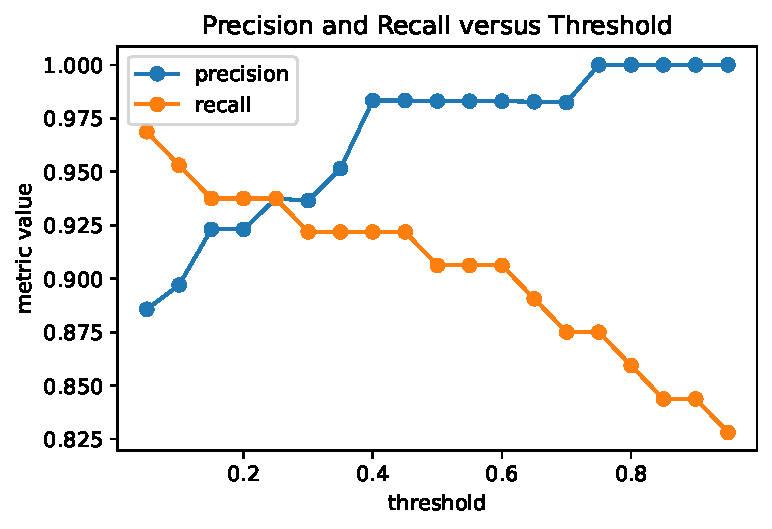
\includegraphics[keepaspectratio]{contents/0/decisioneval_files/figure-pdf/cell-12-output-1.pdf}}

As the threshold increases, the classifier becomes more conservative in
predicting the positive class. This often reduces false positives and
increases precision, but may also increase false negatives and reduce
recall.

\subsection{Choosing a Threshold from
Costs}\label{choosing-a-threshold-from-costs}

In a medical setting, false negatives may be especially important
because they correspond to missed malignant cases. Suppose a false
negative is 5 times as costly as a false positive:

\[
C_{FN}=5,
\quad
C_{FP}=1.
\]

The decision-theoretic threshold is

\[
c^*
=
\frac{C_{FP}}{C_{FP}+C_{FN}}
=
\frac{1}{1+5}
\approx
0.167.
\]

Then the corresponding result is

\begin{Shaded}
\begin{Highlighting}[]
\NormalTok{cost\_fp }\OperatorTok{=} \DecValTok{1}
\NormalTok{cost\_fn }\OperatorTok{=} \DecValTok{5}

\NormalTok{cost\_threshold }\OperatorTok{=}\NormalTok{ cost\_fp }\OperatorTok{/}\NormalTok{ (cost\_fp }\OperatorTok{+}\NormalTok{ cost\_fn)}

\NormalTok{classification\_summary(}
\NormalTok{    y\_test,}
\NormalTok{    logit\_prob,}
\NormalTok{    threshold}\OperatorTok{=}\NormalTok{cost\_threshold,}
\NormalTok{)}
\end{Highlighting}
\end{Shaded}

\begin{verbatim}
{'threshold': 0.16666666666666666,
 'TP': np.int64(60),
 'FP': np.int64(5),
 'FN': np.int64(4),
 'TN': np.int64(102),
 'accuracy': 0.9473684210526315,
 'precision': 0.9230769230769231,
 'recall': 0.9375,
 'f1': 0.9302325581395349}
\end{verbatim}

This lower threshold prioritizes recall. It predicts malignant more
aggressively because missing a malignant tumor is assumed to be more
costly. Note that this threshold formula assumes that the predicted
probabilities are reasonably calibrated so that they can be interpreted
as approximate event probabilities.

\subsection{ROC Curve and AUC}\label{roc-curve-and-auc}

Unlike accuracy or precision, ROC analysis does not depend on a single
fixed threshold. Instead, it studies model performance across all
possible thresholds using the predicted probabilities or scores.

ROC curve and AUC can be computed using \texttt{roc\_curve} and
\texttt{roc\_auc\_score} from \texttt{sklearn.metrics}.

\begin{Shaded}
\begin{Highlighting}[]
\ImportTok{from}\NormalTok{ sklearn.metrics }\ImportTok{import}\NormalTok{ roc\_curve, roc\_auc\_score}

\NormalTok{logit\_fpr, logit\_tpr, \_ }\OperatorTok{=}\NormalTok{ roc\_curve(y\_test, logit\_prob)}
\NormalTok{logit\_auc }\OperatorTok{=}\NormalTok{ roc\_auc\_score(y\_test, logit\_prob)}

\NormalTok{plt.plot(logit\_fpr, logit\_tpr, label}\OperatorTok{=}\SpecialStringTok{f"Logistic regression AUC = }\SpecialCharTok{\{}\NormalTok{logit\_auc}\SpecialCharTok{:.3f\}}\SpecialStringTok{"}\NormalTok{)}
\NormalTok{plt.plot([}\DecValTok{0}\NormalTok{, }\DecValTok{1}\NormalTok{], [}\DecValTok{0}\NormalTok{, }\DecValTok{1}\NormalTok{], }\StringTok{"k{-}{-}"}\NormalTok{, label}\OperatorTok{=}\StringTok{"random guessing"}\NormalTok{)}
\NormalTok{plt.xlabel(}\StringTok{"false positive rate"}\NormalTok{)}
\NormalTok{plt.ylabel(}\StringTok{"true positive rate"}\NormalTok{)}
\NormalTok{plt.title(}\StringTok{"ROC Curve"}\NormalTok{)}
\NormalTok{plt.legend()}
\end{Highlighting}
\end{Shaded}

\pandocbounded{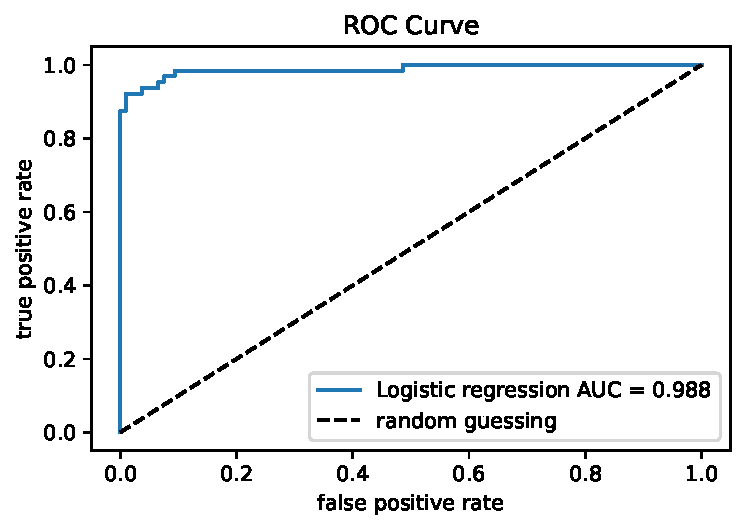
\includegraphics[keepaspectratio]{contents/0/decisioneval_files/figure-pdf/cell-14-output-1.pdf}}

We may fit another model and draw their ROC curve and AUC together in
one plot to compare them.

\begin{Shaded}
\begin{Highlighting}[]
\ImportTok{from}\NormalTok{ sklearn.ensemble }\ImportTok{import}\NormalTok{ RandomForestClassifier}

\NormalTok{rf }\OperatorTok{=}\NormalTok{ RandomForestClassifier(}
\NormalTok{    n\_estimators}\OperatorTok{=}\DecValTok{500}\NormalTok{, max\_features}\OperatorTok{=}\StringTok{"sqrt"}\NormalTok{, random\_state}\OperatorTok{=}\DecValTok{1}\NormalTok{, n\_jobs}\OperatorTok{={-}}\DecValTok{1}
\NormalTok{)}

\NormalTok{rf.fit(X\_train, y\_train)}
\NormalTok{rf\_prob }\OperatorTok{=}\NormalTok{ rf.predict\_proba(X\_test)[:, }\DecValTok{1}\NormalTok{]}

\NormalTok{rf\_fpr, rf\_tpr, \_ }\OperatorTok{=}\NormalTok{ roc\_curve(y\_test, rf\_prob)}
\NormalTok{rf\_auc }\OperatorTok{=}\NormalTok{ roc\_auc\_score(y\_test, rf\_prob)}

\NormalTok{plt.plot(logit\_fpr, logit\_tpr, label}\OperatorTok{=}\SpecialStringTok{f"Logistic regression AUC = }\SpecialCharTok{\{}\NormalTok{logit\_auc}\SpecialCharTok{:.3f\}}\SpecialStringTok{"}\NormalTok{)}
\NormalTok{plt.plot(rf\_fpr, rf\_tpr, label}\OperatorTok{=}\SpecialStringTok{f"Random forest AUC = }\SpecialCharTok{\{}\NormalTok{rf\_auc}\SpecialCharTok{:.3f\}}\SpecialStringTok{"}\NormalTok{)}
\NormalTok{plt.plot([}\DecValTok{0}\NormalTok{, }\DecValTok{1}\NormalTok{], [}\DecValTok{0}\NormalTok{, }\DecValTok{1}\NormalTok{], }\StringTok{"k{-}{-}"}\NormalTok{, label}\OperatorTok{=}\StringTok{"random guessing"}\NormalTok{)}
\NormalTok{plt.xlabel(}\StringTok{"false positive rate"}\NormalTok{)}
\NormalTok{plt.ylabel(}\StringTok{"true positive rate"}\NormalTok{)}
\NormalTok{plt.title(}\StringTok{"ROC Curve"}\NormalTok{)}
\NormalTok{plt.legend()}
\end{Highlighting}
\end{Shaded}

\pandocbounded{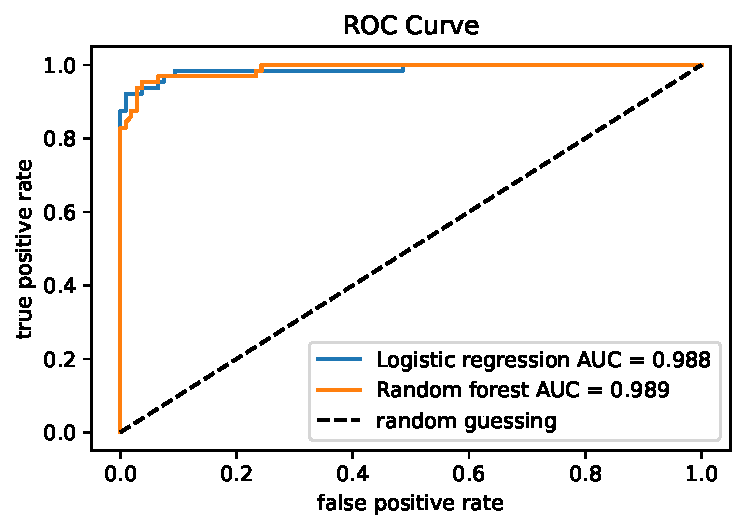
\includegraphics[keepaspectratio]{contents/0/decisioneval_files/figure-pdf/cell-15-output-1.pdf}}

The ROC curve summarizes ranking performance across thresholds. AUC may
be interpreted as the probability that a randomly chosen positive
observation receives a higher score than a randomly chosen negative
observation. Then a larger AUC means the model more often ranks
malignant cases above benign cases.

\subsection{Precision-Recall Curve}\label{precision-recall-curve-1}

The precision-recall curve can be produced in a similar way.

\begin{Shaded}
\begin{Highlighting}[]
\ImportTok{from}\NormalTok{ sklearn.metrics }\ImportTok{import}\NormalTok{ precision\_recall\_curve, average\_precision\_score}

\NormalTok{logit\_precision, logit\_recall, \_ }\OperatorTok{=}\NormalTok{ precision\_recall\_curve(y\_test, logit\_prob)}
\NormalTok{rf\_precision, rf\_recall, \_ }\OperatorTok{=}\NormalTok{ precision\_recall\_curve(y\_test, rf\_prob)}

\NormalTok{logit\_ap }\OperatorTok{=}\NormalTok{ average\_precision\_score(y\_test, logit\_prob)}
\NormalTok{rf\_ap }\OperatorTok{=}\NormalTok{ average\_precision\_score(y\_test, rf\_prob)}

\NormalTok{plt.plot(logit\_recall, logit\_precision, label}\OperatorTok{=}\SpecialStringTok{f"Logistic regression AP = }\SpecialCharTok{\{}\NormalTok{logit\_ap}\SpecialCharTok{:.3f\}}\SpecialStringTok{"}\NormalTok{)}
\NormalTok{plt.plot(rf\_recall, rf\_precision, label}\OperatorTok{=}\SpecialStringTok{f"Random forest AP = }\SpecialCharTok{\{}\NormalTok{rf\_ap}\SpecialCharTok{:.3f\}}\SpecialStringTok{"}\NormalTok{)}
\NormalTok{plt.xlabel(}\StringTok{"recall"}\NormalTok{)}
\NormalTok{plt.ylabel(}\StringTok{"precision"}\NormalTok{)}
\NormalTok{plt.title(}\StringTok{"Precision{-}Recall Curve"}\NormalTok{)}
\NormalTok{plt.legend()}
\end{Highlighting}
\end{Shaded}

\pandocbounded{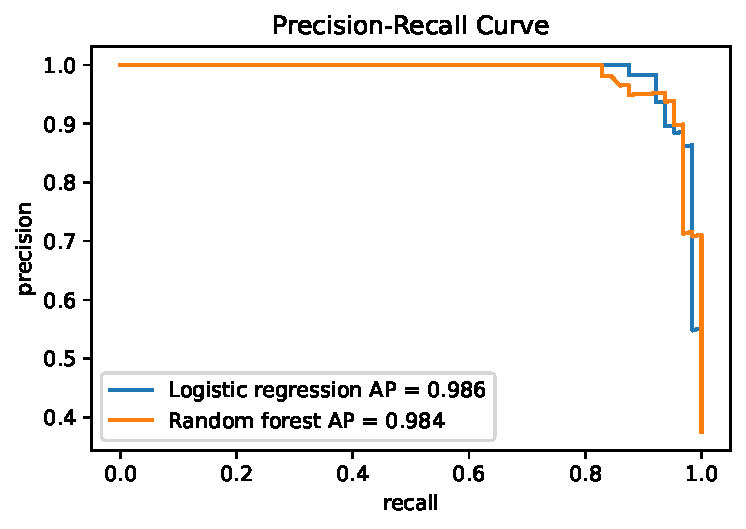
\includegraphics[keepaspectratio]{contents/0/decisioneval_files/figure-pdf/cell-16-output-1.pdf}}

For highly imbalanced datasets, precision--recall curves are often more
informative than ROC curves because ROC curves may appear overly
optimistic when the negative class dominates.

\subsection{Optional: Calibration
Curves}\label{optional-calibration-curves}

Click to expand.

Calibration focuses on probability quality rather than threshold-based
decision quality or ranking quality. Calibration curves can be produced
using \texttt{CalibrationDisplay} from \texttt{sklearn.calibration}.

\begin{Shaded}
\begin{Highlighting}[]
\ImportTok{from}\NormalTok{ sklearn.calibration }\ImportTok{import}\NormalTok{ CalibrationDisplay}

\NormalTok{CalibrationDisplay.from\_predictions(y\_test, logit\_prob, n\_bins}\OperatorTok{=}\DecValTok{10}\NormalTok{)}
\NormalTok{plt.title(}\StringTok{"Calibration Curve"}\NormalTok{)}\OperatorTok{;}
\end{Highlighting}
\end{Shaded}

\pandocbounded{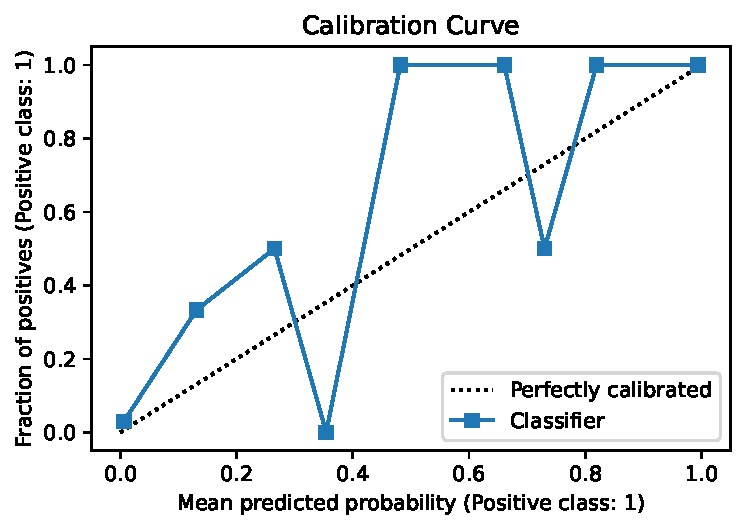
\includegraphics[keepaspectratio]{contents/0/decisioneval_files/figure-pdf/cell-17-output-1.pdf}}

This is a packaged function provided by \texttt{sklearn}. If we want to
plot multiple curves together in one plot, we can put the axis in the
argument of this function.

\begin{Shaded}
\begin{Highlighting}[]
\NormalTok{fig, ax }\OperatorTok{=}\NormalTok{ plt.subplots()}

\NormalTok{CalibrationDisplay.from\_predictions(}
\NormalTok{    y\_test, logit\_prob, n\_bins}\OperatorTok{=}\DecValTok{10}\NormalTok{, name}\OperatorTok{=}\StringTok{"Logistic regression"}\NormalTok{, ax}\OperatorTok{=}\NormalTok{ax}
\NormalTok{)}

\NormalTok{CalibrationDisplay.from\_predictions(}
\NormalTok{    y\_test, rf\_prob, n\_bins}\OperatorTok{=}\DecValTok{10}\NormalTok{, name}\OperatorTok{=}\StringTok{"Random forest"}\NormalTok{, ax}\OperatorTok{=}\NormalTok{ax}
\NormalTok{)}
\end{Highlighting}
\end{Shaded}

\pandocbounded{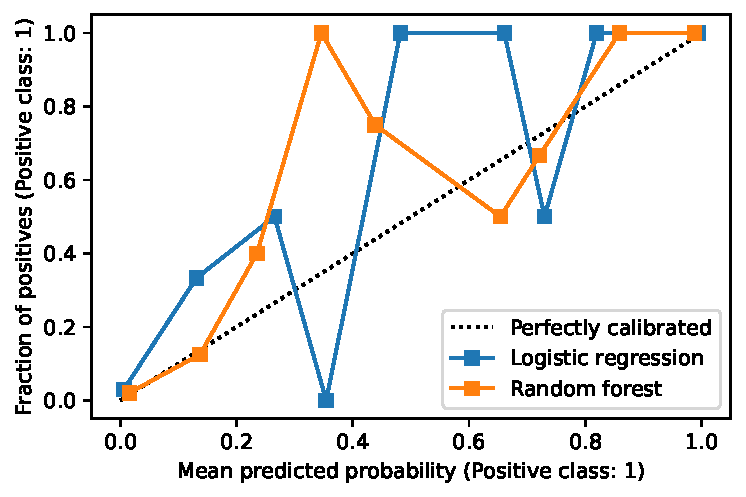
\includegraphics[keepaspectratio]{contents/0/decisioneval_files/figure-pdf/cell-18-output-1.pdf}}

The calibration curve compares predicted probabilities with observed
frequencies.

Calibration curves diagnose probability quality; they do not by
themselves recalibrate the model. Recalibration methods such as Platt
scaling or isotonic regression can change the probability scale, but
they do not necessarily improve AUC because AUC mainly depends on
ranking.

\part{Parametric Supervised Learning}

\chapter{Linear Regression}\label{linear-regression}

This section offers a brief review of linear regression, with the main
emphasis on its Python implementation through examples.

\section{Quick Overview}\label{quick-overview}

Linear regression is the fundamental supervised learning method for a
quantitative response. It models the conditional mean of the response as
a linear function of the predictors: \[
y = \beta_0 + \beta_1 x_1 + \cdots + \beta_p x_p + \varepsilon.
\]

In matrix notation, this can be written as \[
\vb y = \vb X\beta + \varepsilon.
\] Here, \(\vb X\) is the design matrix, whose first column is a column
of ones representing the intercept.

\section{The Ordinary Least Squares
Estimator}\label{the-ordinary-least-squares-estimator}

The most common fitting method is ordinary least squares (OLS). It
chooses the coefficient vector \(\beta\) that minimizes the residual sum
of squares (\(\rss\)):

\[
\rss(\beta) = \sum_{i=1}^n (y_i - \hat{y}_i)^2
= \norm{\vb y - \vb X\beta }_2^2.
\]

\begin{theorem}[OLS Estimator]\protect\hypertarget{thm-}{}\label{thm-}

The coefficient vector that minimizes \(\rss\) is \[
\hat{\beta}_{\ols} = (\vb X^\top \vb X)^{-1}\vb X^\top \vb y,
\] provided that \(\vb X^\top \vb X\) is invertible. This estimator is
called the ordinary least squares (OLS) estimator.

\end{theorem}

Once the coefficients are estimated, the fitted value for observation
\(i\) is

\[
\hat{y}_i = \hat{\beta}_0 + \hat{\beta}_1 x_{i1} + \cdots + \hat{\beta}_p x_{ip}.
\]

Interpretability is one of the main advantages of linear regression
compared with many more complex models.

\begin{enumerate}
\def\labelenumi{\arabic{enumi}.}
\tightlist
\item
  The coefficient \(\hat\beta_j\) describes how the predicted response
  changes when \(x_j\) increases by one unit, while the other predictors
  are held fixed.
\item
  When interaction terms are present, a main effect cannot be
  interpreted in isolation. The effect of a predictor depends on the
  values of the variables with which it interacts.
\item
  If predictors are centered so that \(0\) corresponds to the average of
  the original variable, the intercept represents the predicted response
  at the average predictor levels.
\end{enumerate}

\begin{tcolorbox}[enhanced jigsaw, arc=.35mm, bottomrule=.15mm, bottomtitle=1mm, breakable, colback=white, colbacktitle=quarto-callout-note-color!10!white, colframe=quarto-callout-note-color-frame, coltitle=black, left=2mm, leftrule=.75mm, opacityback=0, opacitybacktitle=0.6, rightrule=.15mm, title=\textcolor{quarto-callout-note-color}{\faInfo}\hspace{0.5em}{Note}, titlerule=0mm, toprule=.15mm, toptitle=1mm]

Classical regression primarily focuses on inference and model
assumptions, such as normality, constant variance, and independence of
errors.

As discussed earlier in the statistical learning basics section,
statistical learning places greater emphasis on predictive performance
and generalization to unseen data. As a result, estimated test error and
model validation often play a more central role than formal inference
procedures.

\end{tcolorbox}

\section{Linear Regression in Python}\label{linear-regression-in-python}

There are many Python libraries for fitting linear regression models. In
this course, we use
\href{https://scikit-learn.org/}{\texttt{scikit-learn}} as the primary
modeling tool, with support from \texttt{pandas} and \texttt{numpy} for
data manipulation, and \texttt{matplotlib} and \texttt{seaborn} for
visualization.

To demonstrate the code, we generate a dataset with 2 predictors and 1
response variable, where \(\beta_0 = 1\), \(\beta_1 = 2\), and
\(\beta_2 = 3\).

\begin{Shaded}
\begin{Highlighting}[]
\ImportTok{import}\NormalTok{ numpy }\ImportTok{as}\NormalTok{ np}
\ImportTok{import}\NormalTok{ pandas }\ImportTok{as}\NormalTok{ pd}

\NormalTok{n }\OperatorTok{=} \DecValTok{100}

\NormalTok{rng }\OperatorTok{=}\NormalTok{ np.random.default\_rng(}\DecValTok{1}\NormalTok{)}

\NormalTok{x1 }\OperatorTok{=}\NormalTok{ rng.normal(}\DecValTok{1}\NormalTok{, }\FloatTok{0.1}\NormalTok{, size}\OperatorTok{=}\NormalTok{n)}
\NormalTok{x2 }\OperatorTok{=}\NormalTok{ rng.normal(}\DecValTok{0}\NormalTok{, }\DecValTok{1}\NormalTok{, size}\OperatorTok{=}\NormalTok{n)}
\NormalTok{y }\OperatorTok{=} \DecValTok{1} \OperatorTok{+} \DecValTok{2} \OperatorTok{*}\NormalTok{ x1 }\OperatorTok{+} \DecValTok{3} \OperatorTok{*}\NormalTok{ x2 }\OperatorTok{+}\NormalTok{ rng.normal(}\DecValTok{0}\NormalTok{, }\FloatTok{0.5}\NormalTok{, size}\OperatorTok{=}\NormalTok{n)}

\NormalTok{X }\OperatorTok{=}\NormalTok{ pd.DataFrame(\{}\StringTok{\textquotesingle{}x1\textquotesingle{}}\NormalTok{: x1, }\StringTok{\textquotesingle{}x2\textquotesingle{}}\NormalTok{: x2\})}
\end{Highlighting}
\end{Shaded}

When using \texttt{sklearn}, a dataset is typically represented by
features \texttt{X} and a target variable \texttt{y}.

\begin{itemize}
\tightlist
\item
  \texttt{X} usually has 2 dimensions (number of samples × features).
\item
  \texttt{y} is usually 1-dimensional, though it may also be represented
  as a 2-dimensional array with a single column.
\end{itemize}

Both \texttt{X} and \texttt{y} can be stored as either \texttt{numpy}
arrays or \texttt{pandas} objects.

In this example we construct \texttt{X} as a DataFrame, since column
names make it easier to modify variables during the model-building
stage, e.g.~when adding interactions or transformations.

\subsection{Linear regression models}\label{linear-regression-models}

We fit a linear regression model using \texttt{LinearRegression}.

\begin{Shaded}
\begin{Highlighting}[]
\ImportTok{from}\NormalTok{ sklearn.linear\_model }\ImportTok{import}\NormalTok{ LinearRegression}

\NormalTok{model }\OperatorTok{=}\NormalTok{ LinearRegression()}
\NormalTok{model.fit(X, y)}

\BuiltInTok{print}\NormalTok{(}\SpecialStringTok{f"intercept: }\SpecialCharTok{\{}\NormalTok{model}\SpecialCharTok{.}\NormalTok{intercept\_}\SpecialCharTok{\}}\SpecialStringTok{"}\NormalTok{)}
\BuiltInTok{print}\NormalTok{(}\SpecialStringTok{f"coefficients: }\SpecialCharTok{\{}\NormalTok{model}\SpecialCharTok{.}\NormalTok{coef\_}\SpecialCharTok{\}}\SpecialStringTok{"}\NormalTok{)}
\end{Highlighting}
\end{Shaded}

\begin{verbatim}
intercept: 0.9846240766122039
coefficients: [1.93387446 2.99292344]
\end{verbatim}

We can then use the fitted model to generate predictions and compute
residuals.

\begin{Shaded}
\begin{Highlighting}[]
\NormalTok{y\_pred }\OperatorTok{=}\NormalTok{ model.predict(X)}
\NormalTok{res }\OperatorTok{=}\NormalTok{ y }\OperatorTok{{-}}\NormalTok{ y\_pred}
\end{Highlighting}
\end{Shaded}

\subsection{Measure model performance}\label{measure-model-performance}

\texttt{sklearn} provides many performance measures, most of which can
be found in \texttt{sklearn.metrics}. A common syntax is
\texttt{metric(y\_true,\ y\_pred)}.

\begin{Shaded}
\begin{Highlighting}[]
\ImportTok{from}\NormalTok{ sklearn.metrics }\ImportTok{import}\NormalTok{ mean\_squared\_error, r2\_score, root\_mean\_squared\_error}

\NormalTok{y\_pred }\OperatorTok{=}\NormalTok{ model.predict(X)}

\BuiltInTok{print}\NormalTok{(}\SpecialStringTok{f"MSE: }\SpecialCharTok{\{}\NormalTok{mean\_squared\_error(y, y\_pred)}\SpecialCharTok{\}}\SpecialStringTok{"}\NormalTok{)}
\BuiltInTok{print}\NormalTok{(}\SpecialStringTok{f"R2: }\SpecialCharTok{\{}\NormalTok{r2\_score(y, y\_pred)}\SpecialCharTok{\}}\SpecialStringTok{"}\NormalTok{)}
\BuiltInTok{print}\NormalTok{(}\SpecialStringTok{f"RMSE: }\SpecialCharTok{\{}\NormalTok{root\_mean\_squared\_error(y, y\_pred)}\SpecialCharTok{\}}\SpecialStringTok{"}\NormalTok{)}
\end{Highlighting}
\end{Shaded}

Each model also provides a built-in scoring method. For a specific
model, you can check the official documentation to see which metric is
used, but the general idea is:

\begin{itemize}
\tightlist
\item
  regressors use \texttt{r2\_score}, and
\item
  classifiers use \texttt{accuracy}
\end{itemize}

\begin{Shaded}
\begin{Highlighting}[]
\NormalTok{model.score(X, y)}
\end{Highlighting}
\end{Shaded}

\begin{verbatim}
0.9769128696597689
\end{verbatim}

\begin{tcolorbox}[enhanced jigsaw, arc=.35mm, bottomrule=.15mm, bottomtitle=1mm, breakable, colback=white, colbacktitle=quarto-callout-note-color!10!white, colframe=quarto-callout-note-color-frame, coltitle=black, left=2mm, leftrule=.75mm, opacityback=0, opacitybacktitle=0.6, rightrule=.15mm, title=\textcolor{quarto-callout-note-color}{\faInfo}\hspace{0.5em}{Different Definitions Across Software}, titlerule=0mm, toprule=.15mm, toptitle=1mm]

Some evaluation metrics may be defined slightly differently across
software packages and textbooks.

For example, mean squared error (MSE) in statistics is defined as
\(\frac{\mathrm{RSS}}{n-(p+1)}\) where \((p+1)\) is the number of
estimated parameters. This adjustment accounts for the degrees of
freedom used in fitting the model.

In contrast, MSE in machine learning (and \texttt{sklearn}) are commonly
defined as \(\frac{\mathrm{RSS}}{n}\) which is simply the average
squared prediction error over the observations.

These differences are usually small when the sample size is large, but
they can affect numerical comparisons between software packages or
published benchmarks. Therefore, it is important to verify the exact
definition of any metric before making comparisons.

For example, according to the \texttt{sklearn}
\href{https://scikit-learn.org/stable/modules/model_evaluation.html\#mean-squared-error}{documentation},
\texttt{mean\_squared\_error} is computed by averaging over the number
of samples \(n\).

\end{tcolorbox}

\subsection{Model Diagnostics}\label{model-diagnostics}

In traditional regression, diagnostic plots are powerful tools for
detecting potential problems in a fitted model. However, statistical
learning primarily focuses on prediction performance rather than model
assumptions. Therefore, diagnostics are not our primary focus in this
course, and this section is optional.

Click for more details.

In Python there is no single function that automatically produces all
diagnostic plots. Instead, we usually combine tools from several
libraries. In these notes we focus on basic tools from
\texttt{statsmodels}, \texttt{scipy}, \texttt{seaborn}, and
\texttt{matplotlib}.

We can also use \texttt{seaborn}'s theme to improve the appearance of
plots produced by \texttt{matplotlib}-based tools.

\begin{Shaded}
\begin{Highlighting}[]
\ImportTok{import}\NormalTok{ seaborn }\ImportTok{as}\NormalTok{ sns}
\NormalTok{sns.set\_theme()}
\end{Highlighting}
\end{Shaded}

We compute several quantities needed for residual analysis. Although our
primary modeling tool is \texttt{sklearn}, residual diagnostics are
easier with \texttt{statsmodels}. Therefore we construct a
\texttt{statsmodels} model that holds the same data.

Since we already have the feature matrix and the target vector, the
fastest way to use \texttt{statsmodels} is through
\texttt{statsmodels.api} (as opposed to the R-style interface
\texttt{statsmodels.formula.api}).

\begin{Shaded}
\begin{Highlighting}[]
\ImportTok{import}\NormalTok{ statsmodels.api }\ImportTok{as}\NormalTok{ sm}
\NormalTok{X\_sm }\OperatorTok{=}\NormalTok{ sm.add\_constant(X)}
\NormalTok{model }\OperatorTok{=}\NormalTok{ sm.OLS(y, X\_sm).fit()}
\NormalTok{model.params}
\end{Highlighting}
\end{Shaded}

\begin{verbatim}
const    0.984624
x1       1.933874
x2       2.992923
dtype: float64
\end{verbatim}

The fitted values, residuals, leverage, Cook's distance, and other
quantities can be extracted directly from this \texttt{model} object. We
wrap them into DataFrames for easier plotting.

\begin{Shaded}
\begin{Highlighting}[]
\NormalTok{y\_pred }\OperatorTok{=}\NormalTok{ model.fittedvalues}
\NormalTok{res }\OperatorTok{=}\NormalTok{ model.resid}

\NormalTok{model\_output }\OperatorTok{=}\NormalTok{ pd.DataFrame(\{}
    \StringTok{"y\_true"}\NormalTok{: y,}
    \StringTok{"y\_pred"}\NormalTok{: y\_pred,}
    \StringTok{"res"}\NormalTok{: res}
\NormalTok{\})}
\end{Highlighting}
\end{Shaded}

\begin{Shaded}
\begin{Highlighting}[]
\NormalTok{influence }\OperatorTok{=}\NormalTok{ model.get\_influence()}

\NormalTok{std\_resid }\OperatorTok{=}\NormalTok{ influence.resid\_studentized\_internal}
\NormalTok{sqrt\_std\_resid }\OperatorTok{=}\NormalTok{ np.sqrt(np.}\BuiltInTok{abs}\NormalTok{(std\_resid))}
\NormalTok{leverage }\OperatorTok{=}\NormalTok{ influence.hat\_matrix\_diag}
\NormalTok{cooks }\OperatorTok{=}\NormalTok{ influence.cooks\_distance[}\DecValTok{0}\NormalTok{]}

\NormalTok{df\_diag }\OperatorTok{=}\NormalTok{ pd.DataFrame(\{}
    \StringTok{"leverage"}\NormalTok{: leverage,}
    \StringTok{"std\_resid"}\NormalTok{: std\_resid,}
    \StringTok{"sqrt\_std\_resid"}\NormalTok{: sqrt\_std\_resid,}
    \StringTok{"cooks"}\NormalTok{: cooks}
\NormalTok{\})}
\end{Highlighting}
\end{Shaded}

\begin{tcolorbox}[enhanced jigsaw, arc=.35mm, bottomrule=.15mm, bottomtitle=1mm, breakable, colback=white, colbacktitle=quarto-callout-note-color!10!white, colframe=quarto-callout-note-color-frame, coltitle=black, left=2mm, leftrule=.75mm, opacityback=0, opacitybacktitle=0.6, rightrule=.15mm, title=\textcolor{quarto-callout-note-color}{\faInfo}\hspace{0.5em}{Residual plots}, titlerule=0mm, toprule=.15mm, toptitle=1mm]

The most basic residual plot is simply residuals versus fitted values.

\begin{Shaded}
\begin{Highlighting}[]
\ImportTok{import}\NormalTok{ matplotlib.pyplot }\ImportTok{as}\NormalTok{ plt}

\NormalTok{plt.scatter(y\_pred, res)}
\NormalTok{plt.axhline(}\DecValTok{0}\NormalTok{, linestyle}\OperatorTok{=}\StringTok{"{-}{-}"}\NormalTok{)}
\end{Highlighting}
\end{Shaded}

\pandocbounded{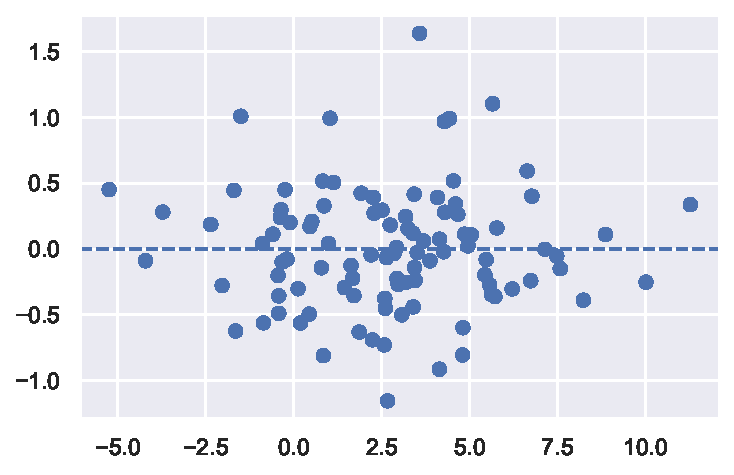
\includegraphics[keepaspectratio]{contents/1/lr_files/figure-pdf/cell-11-output-1.pdf}}

If we use \texttt{seaborn}, additional features are computed
automatically. For example, setting \texttt{lowess=True} will display a
smooth trend curve.

\begin{Shaded}
\begin{Highlighting}[]
\ImportTok{import}\NormalTok{ seaborn }\ImportTok{as}\NormalTok{ sns}

\NormalTok{sns.regplot(}
\NormalTok{    data}\OperatorTok{=}\NormalTok{model\_output,}
\NormalTok{    x}\OperatorTok{=}\StringTok{"y\_pred"}\NormalTok{,}
\NormalTok{    y}\OperatorTok{=}\StringTok{"res"}\NormalTok{,}
\NormalTok{    lowess}\OperatorTok{=}\VariableTok{True}\NormalTok{,}
\NormalTok{    scatter\_kws}\OperatorTok{=}\NormalTok{\{}\StringTok{"alpha"}\NormalTok{: }\FloatTok{0.6}\NormalTok{\},}
\NormalTok{    line\_kws}\OperatorTok{=}\NormalTok{\{}\StringTok{"color"}\NormalTok{: }\StringTok{"red"}\NormalTok{, }\StringTok{"linestyle"}\NormalTok{: }\StringTok{"{-}{-}"}\NormalTok{\},}
\NormalTok{)}

\NormalTok{plt.axhline(}\DecValTok{0}\NormalTok{, linestyle}\OperatorTok{=}\StringTok{"{-}{-}"}\NormalTok{)}
\end{Highlighting}
\end{Shaded}

\pandocbounded{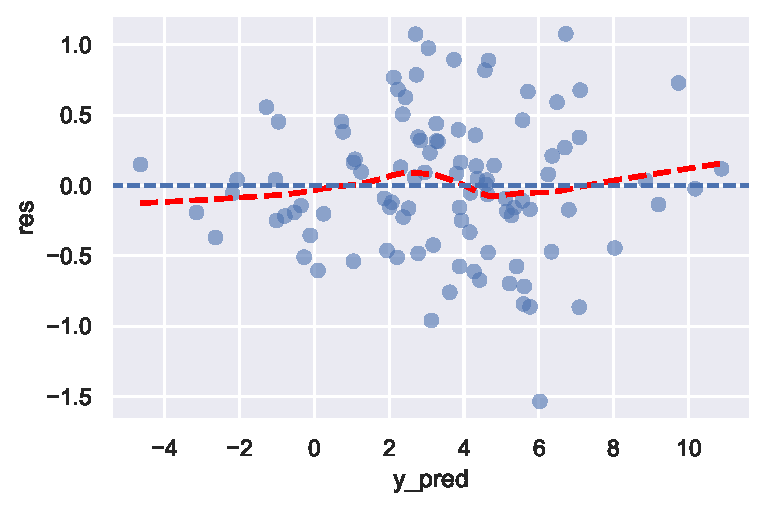
\includegraphics[keepaspectratio]{contents/1/lr_files/figure-pdf/cell-12-output-1.pdf}}

\end{tcolorbox}

\begin{tcolorbox}[enhanced jigsaw, arc=.35mm, bottomrule=.15mm, bottomtitle=1mm, breakable, colback=white, colbacktitle=quarto-callout-note-color!10!white, colframe=quarto-callout-note-color-frame, coltitle=black, left=2mm, leftrule=.75mm, opacityback=0, opacitybacktitle=0.6, rightrule=.15mm, title=\textcolor{quarto-callout-note-color}{\faInfo}\hspace{0.5em}{Q-Q plot}, titlerule=0mm, toprule=.15mm, toptitle=1mm]

\begin{Shaded}
\begin{Highlighting}[]
\ImportTok{import}\NormalTok{ scipy.stats }\ImportTok{as}\NormalTok{ stats}

\NormalTok{stats.probplot(res, dist}\OperatorTok{=}\StringTok{"norm"}\NormalTok{, plot}\OperatorTok{=}\NormalTok{plt)}\OperatorTok{;}
\end{Highlighting}
\end{Shaded}

\pandocbounded{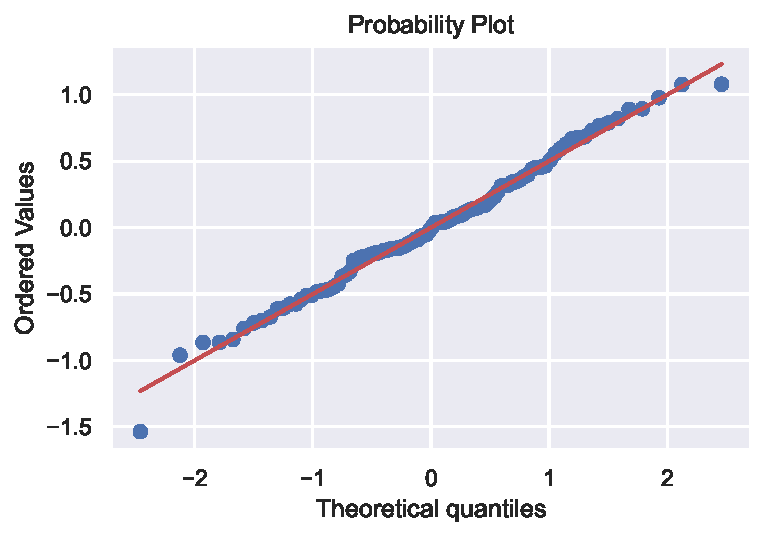
\includegraphics[keepaspectratio]{contents/1/lr_files/figure-pdf/cell-13-output-1.pdf}}

\end{tcolorbox}

\begin{tcolorbox}[enhanced jigsaw, arc=.35mm, bottomrule=.15mm, bottomtitle=1mm, breakable, colback=white, colbacktitle=quarto-callout-note-color!10!white, colframe=quarto-callout-note-color-frame, coltitle=black, left=2mm, leftrule=.75mm, opacityback=0, opacitybacktitle=0.6, rightrule=.15mm, title=\textcolor{quarto-callout-note-color}{\faInfo}\hspace{0.5em}{Scale-location plot}, titlerule=0mm, toprule=.15mm, toptitle=1mm]

\begin{Shaded}
\begin{Highlighting}[]
\ImportTok{import}\NormalTok{ numpy }\ImportTok{as}\NormalTok{ np}


\NormalTok{sns.scatterplot(x}\OperatorTok{=}\NormalTok{y\_pred, y}\OperatorTok{=}\NormalTok{sqrt\_std\_resid, data}\OperatorTok{=}\NormalTok{df\_diag)}

\NormalTok{sns.regplot(}
\NormalTok{    x}\OperatorTok{=}\NormalTok{y\_pred,}
\NormalTok{    y}\OperatorTok{=}\NormalTok{sqrt\_std\_resid,}
\NormalTok{    data}\OperatorTok{=}\NormalTok{df\_diag,}
\NormalTok{    lowess}\OperatorTok{=}\VariableTok{True}\NormalTok{,}
\NormalTok{    scatter}\OperatorTok{=}\VariableTok{False}\NormalTok{,}
\NormalTok{    line\_kws}\OperatorTok{=}\NormalTok{\{}\StringTok{"color"}\NormalTok{: }\StringTok{"red"}\NormalTok{\}}
\NormalTok{)}

\NormalTok{plt.xlabel(}\StringTok{"Fitted values"}\NormalTok{)}
\NormalTok{plt.ylabel(}\StringTok{"√|Standardized residuals|"}\NormalTok{)}
\NormalTok{plt.title(}\StringTok{"Scale{-}Location"}\NormalTok{)}\OperatorTok{;}
\end{Highlighting}
\end{Shaded}

\pandocbounded{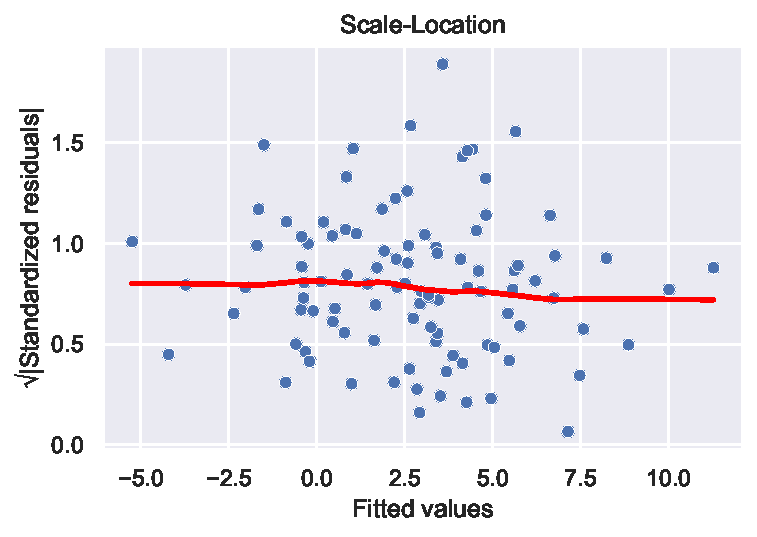
\includegraphics[keepaspectratio]{contents/1/lr_files/figure-pdf/cell-14-output-1.pdf}}

\end{tcolorbox}

\begin{tcolorbox}[enhanced jigsaw, arc=.35mm, bottomrule=.15mm, bottomtitle=1mm, breakable, colback=white, colbacktitle=quarto-callout-note-color!10!white, colframe=quarto-callout-note-color-frame, coltitle=black, left=2mm, leftrule=.75mm, opacityback=0, opacitybacktitle=0.6, rightrule=.15mm, title=\textcolor{quarto-callout-note-color}{\faInfo}\hspace{0.5em}{Leverage with Cook's distance}, titlerule=0mm, toprule=.15mm, toptitle=1mm]

\begin{Shaded}
\begin{Highlighting}[]
\NormalTok{sns.scatterplot(}
\NormalTok{    x}\OperatorTok{=}\NormalTok{leverage,}
\NormalTok{    y}\OperatorTok{=}\NormalTok{std\_resid,}
\NormalTok{    data}\OperatorTok{=}\NormalTok{df\_diag,}
\NormalTok{    size}\OperatorTok{=}\NormalTok{cooks,}
\NormalTok{    sizes}\OperatorTok{=}\NormalTok{(}\DecValTok{20}\NormalTok{, }\DecValTok{200}\NormalTok{),}
\NormalTok{    alpha}\OperatorTok{=}\FloatTok{0.7}
\NormalTok{)}

\NormalTok{plt.axhline(}\DecValTok{0}\NormalTok{, linestyle}\OperatorTok{=}\StringTok{"{-}{-}"}\NormalTok{, color}\OperatorTok{=}\StringTok{"gray"}\NormalTok{)}

\NormalTok{plt.xlabel(}\StringTok{"Leverage"}\NormalTok{)}
\NormalTok{plt.ylabel(}\StringTok{"Standardized Residuals"}\NormalTok{)}
\NormalTok{plt.title(}\StringTok{"Residuals vs Leverage"}\NormalTok{)}\OperatorTok{;}
\end{Highlighting}
\end{Shaded}

\pandocbounded{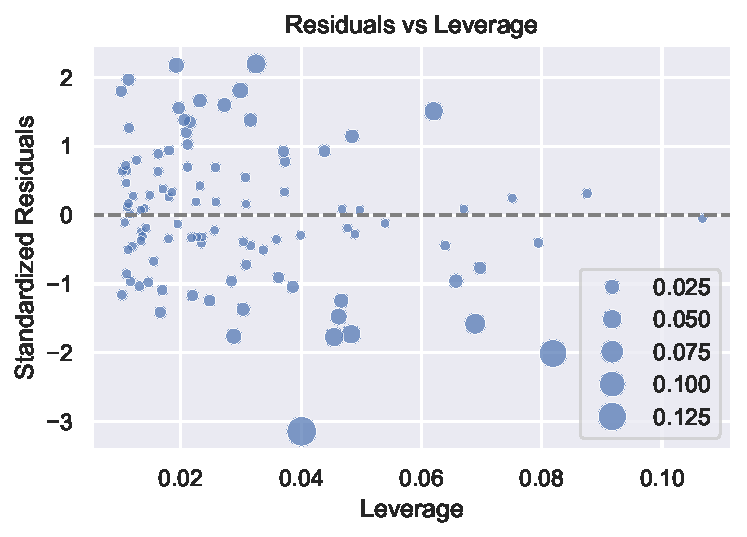
\includegraphics[keepaspectratio]{contents/1/lr_files/figure-pdf/cell-15-output-1.pdf}}

\end{tcolorbox}

\begin{tcolorbox}[enhanced jigsaw, arc=.35mm, bottomrule=.15mm, bottomtitle=1mm, breakable, colback=white, colbacktitle=quarto-callout-note-color!10!white, colframe=quarto-callout-note-color-frame, coltitle=black, left=2mm, leftrule=.75mm, opacityback=0, opacitybacktitle=0.6, rightrule=.15mm, title=\textcolor{quarto-callout-note-color}{\faInfo}\hspace{0.5em}{Partial residual plots}, titlerule=0mm, toprule=.15mm, toptitle=1mm]

Partial residual plots help visualize the relationship between a
predictor and the response after adjusting for the effects of other
predictors. \texttt{plot\_ccpr()} from \texttt{sm.graphics} can be used
to generate partial residual plots.

\begin{Shaded}
\begin{Highlighting}[]
\NormalTok{sm.graphics.plot\_ccpr(model, }\StringTok{"x1"}\NormalTok{)}\OperatorTok{;}
\end{Highlighting}
\end{Shaded}

\pandocbounded{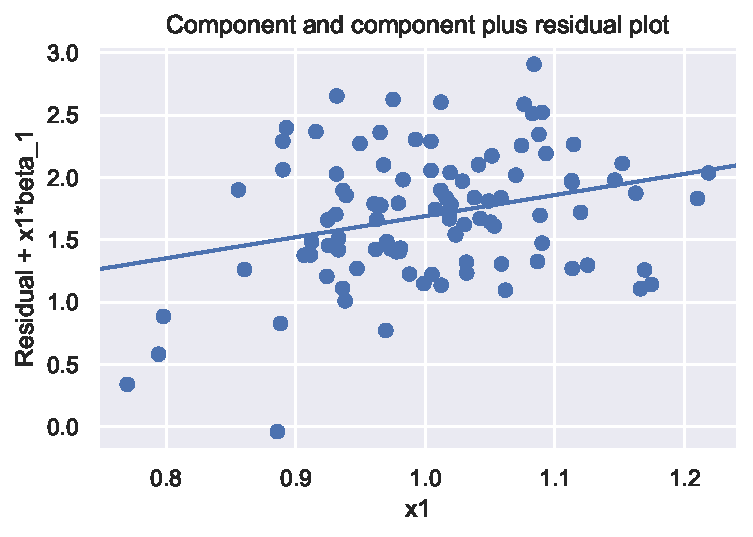
\includegraphics[keepaspectratio]{contents/1/lr_files/figure-pdf/cell-16-output-1.pdf}}

To generate plots for all predictors at once, we can use

\begin{Shaded}
\begin{Highlighting}[]
\NormalTok{sm.graphics.plot\_ccpr\_grid(model)}\OperatorTok{;}
\end{Highlighting}
\end{Shaded}

\pandocbounded{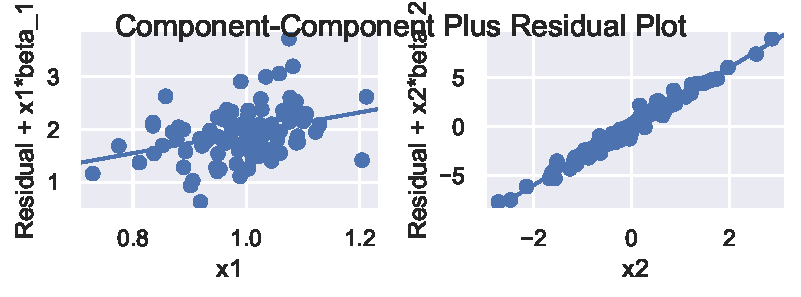
\includegraphics[keepaspectratio]{contents/1/lr_files/figure-pdf/cell-17-output-1.pdf}}

The default \texttt{plot\_ccpr()} does not include a smooth curve. If a
smooth trend line is desired, we can compute it using the
\texttt{lowess()} function and add it manually.

\begin{Shaded}
\begin{Highlighting}[]
\ImportTok{from}\NormalTok{ statsmodels.nonparametric.smoothers\_lowess }\ImportTok{import}\NormalTok{ lowess}

\NormalTok{fig }\OperatorTok{=}\NormalTok{ sm.graphics.plot\_ccpr(model, }\StringTok{"x1"}\NormalTok{)}

\NormalTok{ax }\OperatorTok{=}\NormalTok{ fig.axes[}\DecValTok{0}\NormalTok{]}
\NormalTok{x }\OperatorTok{=}\NormalTok{ ax.lines[}\DecValTok{0}\NormalTok{].get\_xdata()}
\NormalTok{y }\OperatorTok{=}\NormalTok{ ax.lines[}\DecValTok{0}\NormalTok{].get\_ydata()}

\NormalTok{smooth }\OperatorTok{=}\NormalTok{ lowess(y, x, frac}\OperatorTok{=}\FloatTok{0.5}\NormalTok{)}
\NormalTok{ax.plot(smooth[:, }\DecValTok{0}\NormalTok{], smooth[:, }\DecValTok{1}\NormalTok{], color}\OperatorTok{=}\StringTok{"red"}\NormalTok{)}
\end{Highlighting}
\end{Shaded}

\pandocbounded{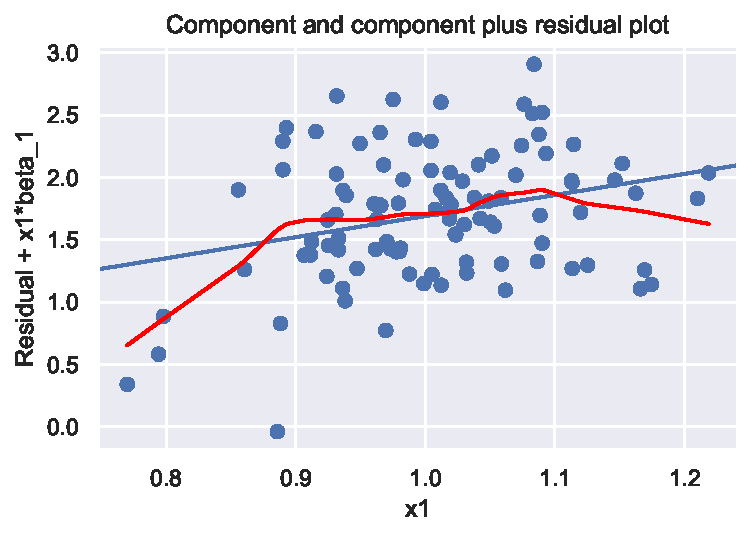
\includegraphics[keepaspectratio]{contents/1/lr_files/figure-pdf/cell-18-output-1.pdf}}

The same idea can be applied to the grid version.

\begin{Shaded}
\begin{Highlighting}[]
\NormalTok{fig }\OperatorTok{=}\NormalTok{ sm.graphics.plot\_ccpr\_grid(model)}

\ControlFlowTok{for}\NormalTok{ ax }\KeywordTok{in}\NormalTok{ fig.axes:}
    \ControlFlowTok{if} \BuiltInTok{len}\NormalTok{(ax.lines) }\OperatorTok{!=} \DecValTok{0}\NormalTok{:}
\NormalTok{        x }\OperatorTok{=}\NormalTok{ ax.lines[}\DecValTok{0}\NormalTok{].get\_xdata()}
\NormalTok{        y }\OperatorTok{=}\NormalTok{ ax.lines[}\DecValTok{0}\NormalTok{].get\_ydata()}

\NormalTok{        smooth }\OperatorTok{=}\NormalTok{ lowess(y, x, frac}\OperatorTok{=}\FloatTok{0.5}\NormalTok{)}
\NormalTok{        ax.plot(smooth[:, }\DecValTok{0}\NormalTok{], smooth[:, }\DecValTok{1}\NormalTok{], color}\OperatorTok{=}\StringTok{"red"}\NormalTok{)}
\end{Highlighting}
\end{Shaded}

\pandocbounded{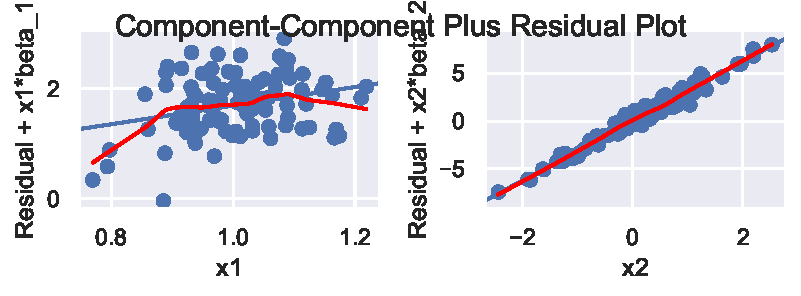
\includegraphics[keepaspectratio]{contents/1/lr_files/figure-pdf/cell-19-output-1.pdf}}

\end{tcolorbox}

\section{Model evaluation}\label{model-evaluation}

\subsection{Train-Test Split}\label{train-test-split}

Instead of estimating test performance indirectly from the training
data, we can evaluate a model more directly by using data that were not
used to fit the model. This leads to the idea of data splitting:

The dataset is divided into two parts:

\begin{itemize}
\tightlist
\item
  Training set: used to fit the model.
\item
  Test set: used to evaluate prediction performance.
\end{itemize}

After fitting the model on the training set, predictions are made on the
test set, and performance measures such as MSE are computed. This
provides a more realistic estimate of how the model performs on new
data.

\begin{center}\rule{0.5\linewidth}{0.5pt}\end{center}

In many situations we also need to choose between several competing
models or tuning parameters. To avoid using the test data for model
selection, a third subset is often introduced.

\begin{itemize}
\tightlist
\item
  Training set: used to fit models.
\item
  Validation set: used to compare models and select tuning parameters.
\item
  Test set: used only once at the end to estimate the final model's
  performance.
\end{itemize}

This separation helps prevent overly optimistic performance estimates.

\begin{center}\rule{0.5\linewidth}{0.5pt}\end{center}

In \texttt{sklearn}, the function \texttt{train\_test\_split()} from
\texttt{sklearn.model\_selection} is commonly used to split the data
into a training set and a test set.

\begin{Shaded}
\begin{Highlighting}[]
\ImportTok{import}\NormalTok{ numpy }\ImportTok{as}\NormalTok{ np}
\ImportTok{import}\NormalTok{ pandas }\ImportTok{as}\NormalTok{ pd}
\ImportTok{from}\NormalTok{ sklearn.model\_selection }\ImportTok{import}\NormalTok{ train\_test\_split}

\NormalTok{n }\OperatorTok{=} \DecValTok{10}

\NormalTok{rng }\OperatorTok{=}\NormalTok{ np.random.default\_rng(}\DecValTok{1}\NormalTok{)}
\NormalTok{x1 }\OperatorTok{=}\NormalTok{ rng.normal(loc}\OperatorTok{=}\DecValTok{1}\NormalTok{, scale}\OperatorTok{=}\FloatTok{0.1}\NormalTok{, size}\OperatorTok{=}\NormalTok{n)}
\NormalTok{x2 }\OperatorTok{=}\NormalTok{ rng.normal(loc}\OperatorTok{=}\DecValTok{0}\NormalTok{, scale}\OperatorTok{=}\DecValTok{1}\NormalTok{, size}\OperatorTok{=}\NormalTok{n)}
\NormalTok{y }\OperatorTok{=} \DecValTok{1} \OperatorTok{+} \DecValTok{2} \OperatorTok{*}\NormalTok{ x1 }\OperatorTok{+} \DecValTok{3} \OperatorTok{*}\NormalTok{ x2 }\OperatorTok{+}\NormalTok{ rng.normal(}\DecValTok{0}\NormalTok{, }\FloatTok{0.5}\NormalTok{, size}\OperatorTok{=}\NormalTok{n)}

\NormalTok{X }\OperatorTok{=}\NormalTok{ pd.DataFrame(\{}\StringTok{\textquotesingle{}x1\textquotesingle{}}\NormalTok{: x1, }\StringTok{\textquotesingle{}x2\textquotesingle{}}\NormalTok{: x2\})}

\NormalTok{X\_train, X\_test, y\_train, y\_test }\OperatorTok{=}\NormalTok{ train\_test\_split(X, y, test\_size}\OperatorTok{=}\FloatTok{0.2}\NormalTok{, random\_state}\OperatorTok{=}\DecValTok{0}\NormalTok{)}
\end{Highlighting}
\end{Shaded}

The argument \texttt{test\_size=0.2} means that 20\% of the data are
used as the test set, while the remaining 80\% are used as the training
set. The argument \texttt{random\_state=0} ensures reproducibility.

\subsection{Cross-Validation}\label{cross-validation}

When the dataset is not large, splitting the data into separate
training, validation, and test sets may leave too little data for model
fitting. In such cases, cross-validation is commonly used to estimate
validation performance more efficiently.

The most common form is \(k\)-fold cross-validation.

\begin{enumerate}
\def\labelenumi{\arabic{enumi}.}
\tightlist
\item
  The available training data are divided into \(k\) roughly equal parts
  (called folds).
\item
  For each fold:

  \begin{itemize}
  \tightlist
  \item
    The model is trained on \(k-1\) folds.
  \item
    The remaining fold is used as a validation set.
  \end{itemize}
\item
  This process is repeated \(k\) times so that each fold serves once as
  the validation set.
\item
  The validation errors from all folds are averaged to estimate the
  model's expected test error.
\end{enumerate}

\begin{center}\rule{0.5\linewidth}{0.5pt}\end{center}

Cross-validation is primarily used to estimate test error or to compare
competing models. When it is used for model selection, two additional
steps are typically performed. Note that cross-validation uses only the
training data and does not involve the test set.

\begin{enumerate}
\def\labelenumi{\arabic{enumi}.}
\setcounter{enumi}{4}
\tightlist
\item
  After the best model configuration has been selected, the model is
  retrained on the entire training data.
\item
  The final model is then evaluated once on the test set, which serves
  as an unbiased estimate of its performance on new data.
\end{enumerate}

\begin{center}\rule{0.5\linewidth}{0.5pt}\end{center}

In \texttt{sklearn}, there are several ways to perform \(k\)-fold
cross-validation. From \texttt{KFold} to \texttt{cross\_validate} and
then \texttt{cross\_val\_score}, the interface becomes easier to use,
but also less flexible.

The three approaches perform essentially the same task, but at different
levels of abstraction.

\begin{tcolorbox}[enhanced jigsaw, arc=.35mm, bottomrule=.15mm, bottomtitle=1mm, breakable, colback=white, colbacktitle=quarto-callout-note-color!10!white, colframe=quarto-callout-note-color-frame, coltitle=black, left=2mm, leftrule=.75mm, opacityback=0, opacitybacktitle=0.6, rightrule=.15mm, title=\textcolor{quarto-callout-note-color}{\faInfo}\hspace{0.5em}{\texttt{KFold}}, titlerule=0mm, toprule=.15mm, toptitle=1mm]

\texttt{KFold} from \texttt{sklearn.model\_selection} is used to split
the dataset into \(k\) groups, called folds. In each iteration, one fold
is used as the validation set and the remaining folds are used as the
training set.

\begin{Shaded}
\begin{Highlighting}[]
\ImportTok{from}\NormalTok{ sklearn.model\_selection }\ImportTok{import}\NormalTok{ KFold}

\NormalTok{kf }\OperatorTok{=}\NormalTok{ KFold(n\_splits}\OperatorTok{=}\DecValTok{5}\NormalTok{)}

\ControlFlowTok{for}\NormalTok{ train\_idx, val\_idx }\KeywordTok{in}\NormalTok{ kf.split(}\BuiltInTok{range}\NormalTok{(}\DecValTok{10}\NormalTok{)):}
    \BuiltInTok{print}\NormalTok{(train\_idx, val\_idx)}
\end{Highlighting}
\end{Shaded}

\begin{verbatim}
[2 3 4 5 6 7 8 9] [0 1]
[0 1 4 5 6 7 8 9] [2 3]
[0 1 2 3 6 7 8 9] [4 5]
[0 1 2 3 4 5 8 9] [6 7]
[0 1 2 3 4 5 6 7] [8 9]
\end{verbatim}

\begin{itemize}
\tightlist
\item
  Here I use \texttt{range(10)} inside \texttt{kf.split()} because only
  the indices are needed. If a dataset is passed instead, the output is
  still the indices for the training set and validation set.
\item
  If you want the split to be randomized, set \texttt{shuffle=True} when
  creating \texttt{KFold}. In that case, you may also specify
  \texttt{random\_state} to make the result reproducible.
\end{itemize}

Let us now apply \texttt{KFold} to our simulated dataset.

\begin{Shaded}
\begin{Highlighting}[]
\ImportTok{from}\NormalTok{ sklearn.model\_selection }\ImportTok{import}\NormalTok{ KFold}
\ImportTok{from}\NormalTok{ sklearn.linear\_model }\ImportTok{import}\NormalTok{ LinearRegression}
\ImportTok{from}\NormalTok{ sklearn.metrics }\ImportTok{import}\NormalTok{ r2\_score}

\NormalTok{kf }\OperatorTok{=}\NormalTok{ KFold(n\_splits}\OperatorTok{=}\DecValTok{5}\NormalTok{, shuffle}\OperatorTok{=}\VariableTok{True}\NormalTok{, random\_state}\OperatorTok{=}\DecValTok{1}\NormalTok{)}

\NormalTok{cv\_scores }\OperatorTok{=}\NormalTok{ []}
\ControlFlowTok{for}\NormalTok{ train\_idx, val\_idx }\KeywordTok{in}\NormalTok{ kf.split(X):}
\NormalTok{    X\_train, X\_val }\OperatorTok{=}\NormalTok{ X.iloc[train\_idx], X.iloc[val\_idx]}
\NormalTok{    y\_train, y\_val }\OperatorTok{=}\NormalTok{ y[train\_idx], y[val\_idx]}

\NormalTok{    model }\OperatorTok{=}\NormalTok{ LinearRegression()}
\NormalTok{    model.fit(X\_train, y\_train)}

\NormalTok{    y\_pred }\OperatorTok{=}\NormalTok{ model.predict(X\_val)}
\NormalTok{    score }\OperatorTok{=}\NormalTok{ r2\_score(y\_val, y\_pred)}

\NormalTok{    cv\_scores.append(score)}

\BuiltInTok{print}\NormalTok{(cv\_scores)}
\BuiltInTok{print}\NormalTok{(}\BuiltInTok{sum}\NormalTok{(cv\_scores) }\OperatorTok{/} \BuiltInTok{len}\NormalTok{(cv\_scores))}
\end{Highlighting}
\end{Shaded}

\begin{verbatim}
[-1.473916411368759, 0.3859310045149441, -0.7579033227389274, 0.7043154482687257, 0.8824788076538627]
-0.051818894734030785
\end{verbatim}

This gives the validation score for each fold, together with their
average.

\end{tcolorbox}

\begin{tcolorbox}[enhanced jigsaw, arc=.35mm, bottomrule=.15mm, bottomtitle=1mm, breakable, colback=white, colbacktitle=quarto-callout-note-color!10!white, colframe=quarto-callout-note-color-frame, coltitle=black, left=2mm, leftrule=.75mm, opacityback=0, opacitybacktitle=0.6, rightrule=.15mm, title=\textcolor{quarto-callout-note-color}{\faInfo}\hspace{0.5em}{\texttt{cross\_validate}}, titlerule=0mm, toprule=.15mm, toptitle=1mm]

Using \texttt{KFold} directly is somewhat manual. We may use
\texttt{cross\_validate()} to automate the cross-validation process.
Depending on the arguments supplied, \texttt{cross\_validate()} may
internally use \texttt{KFold}.

You may specify which scoreing methods useing \texttt{scoring} argument.
The default choice for \texttt{scoring} depends on the model. In
\texttt{LinearRegression} case, the default choice is \texttt{r2}. Note
that this \texttt{scoring} can accept a list of scoring methods, or a
single scoring method.

\begin{Shaded}
\begin{Highlighting}[]
\ImportTok{from}\NormalTok{ sklearn.model\_selection }\ImportTok{import}\NormalTok{ cross\_validate}

\NormalTok{model }\OperatorTok{=}\NormalTok{ LinearRegression()}
\NormalTok{cv\_result }\OperatorTok{=}\NormalTok{ cross\_validate(model, X, y, cv}\OperatorTok{=}\DecValTok{5}\NormalTok{, scoring}\OperatorTok{=}\NormalTok{[}\StringTok{"r2"}\NormalTok{, }\StringTok{"neg\_mean\_squared\_error"}\NormalTok{])}

\NormalTok{cv\_result}
\end{Highlighting}
\end{Shaded}

\begin{verbatim}
{'fit_time': array([0.00148249, 0.00122499, 0.00104594, 0.00093675, 0.00085187]),
 'score_time': array([0.00161695, 0.00092888, 0.00085115, 0.00079632, 0.00077248]),
 'test_r2': array([-0.39366753,  0.10843993,  0.60326202,  0.73431811,  0.91493437]),
 'test_neg_mean_squared_error': array([-0.79253928, -0.34840152, -1.25856101, -0.05339861, -0.05188008])}
\end{verbatim}

If you are only interested in a certain validation scores, you may
extract them directly.

\begin{Shaded}
\begin{Highlighting}[]
\NormalTok{cv\_result[}\StringTok{\textquotesingle{}test\_r2\textquotesingle{}}\NormalTok{]}
\end{Highlighting}
\end{Shaded}

\begin{verbatim}
array([-0.39366753,  0.10843993,  0.60326202,  0.73431811,  0.91493437])
\end{verbatim}

\begin{itemize}
\tightlist
\item
  More info on different scoring methods can be found in
  \href{https://scikit-learn.org/stable/modules/model_evaluation.html\#scoring-parameter}{the
  document}. You can also print it from
  \texttt{sklearn.metrics.get\_scorer\_names()}.
\item
  Here the negative MSE values are negative because \texttt{sklearn}
  follows the convention that larger scores are better.
\item
  If \texttt{cv=5}, then \texttt{KFold(5,\ shuffle=False)} is used by
  default. If you want randomized folds, you may pass a \texttt{KFold}
  object explicitly.
\end{itemize}

\begin{Shaded}
\begin{Highlighting}[]
\NormalTok{cv\_result }\OperatorTok{=}\NormalTok{ cross\_validate(}
\NormalTok{    model, X, y, cv}\OperatorTok{=}\NormalTok{KFold(}\DecValTok{5}\NormalTok{, shuffle}\OperatorTok{=}\VariableTok{True}\NormalTok{, random\_state}\OperatorTok{=}\DecValTok{1}\NormalTok{)}
\NormalTok{)}

\NormalTok{cv\_result[}\StringTok{"test\_score"}\NormalTok{]}
\end{Highlighting}
\end{Shaded}

\begin{verbatim}
array([-1.47391641,  0.385931  , -0.75790332,  0.70431545,  0.88247881])
\end{verbatim}

You may compare these scores with the ones obtained in the
\texttt{KFold} section. Usually, the overall cross-validation score is
taken to be the mean of the fold scores. Note that in this case the
\texttt{scoring} is not given. So it will use the default \(R^2\).

\begin{Shaded}
\begin{Highlighting}[]
\NormalTok{cv\_result[}\StringTok{\textquotesingle{}test\_score\textquotesingle{}}\NormalTok{].mean()}
\end{Highlighting}
\end{Shaded}

\begin{verbatim}
np.float64(-0.051818894734030764)
\end{verbatim}

\end{tcolorbox}

\begin{tcolorbox}[enhanced jigsaw, arc=.35mm, bottomrule=.15mm, bottomtitle=1mm, breakable, colback=white, colbacktitle=quarto-callout-note-color!10!white, colframe=quarto-callout-note-color-frame, coltitle=black, left=2mm, leftrule=.75mm, opacityback=0, opacitybacktitle=0.6, rightrule=.15mm, title=\textcolor{quarto-callout-note-color}{\faInfo}\hspace{0.5em}{\texttt{cross\_val\_score}}, titlerule=0mm, toprule=.15mm, toptitle=1mm]

\texttt{cross\_val\_score()} is a shorter way to obtain
\texttt{cv\_result{[}"test\_score"{]}} from the
\texttt{cross\_validate()} section. The arguments \texttt{cv} and
\texttt{scoring} work in almost the same way, except that
\texttt{scoring} only accept a single scorer instead of a list in this
case.

\begin{Shaded}
\begin{Highlighting}[]
\ImportTok{from}\NormalTok{ sklearn.model\_selection }\ImportTok{import}\NormalTok{ cross\_val\_score}

\NormalTok{cv\_scores }\OperatorTok{=}\NormalTok{ cross\_val\_score(}
\NormalTok{    model, X, y, cv}\OperatorTok{=}\NormalTok{KFold(}\DecValTok{5}\NormalTok{, shuffle}\OperatorTok{=}\VariableTok{True}\NormalTok{, random\_state}\OperatorTok{=}\DecValTok{1}\NormalTok{)}
\NormalTok{)}

\NormalTok{cv\_scores}
\end{Highlighting}
\end{Shaded}

\begin{verbatim}
array([-1.47391641,  0.385931  , -0.75790332,  0.70431545,  0.88247881])
\end{verbatim}

\begin{Shaded}
\begin{Highlighting}[]
\NormalTok{cv\_scores.mean()}
\end{Highlighting}
\end{Shaded}

\begin{verbatim}
np.float64(-0.051818894734030764)
\end{verbatim}

So \texttt{cross\_val\_score()} is convenient when you only need the
validation scores and do not need the extra information returned by
\texttt{cross\_validate()}.

\end{tcolorbox}

\begin{center}\rule{0.5\linewidth}{0.5pt}\end{center}

Cross-validation is often used to compare competing models. One
important application is hyperparameter tuning. In this setting, we
compare models from the same family under different choices of
hyperparameters. In \texttt{sklearn}, this process is commonly carried
out with \texttt{GridSearchCV}.

The CV procedure is summarized (again) as follows:

\begin{enumerate}
\def\labelenumi{\arabic{enumi}.}
\tightlist
\item
  Split the training data into several folds.
\item
  For each hyperparameter combination, hold out one fold as the
  validation set and use the remaining folds as the training set.
\item
  Fit the model on the training folds and evaluate its performance on
  the validation fold.
\item
  Repeat this process so that each fold serves once as the validation
  set. The average validation score is the cross-validation score for
  that hyperparameter combination.
\item
  Repeat Steps 2--4 for all hyperparameter combinations, and select the
  combination with the best average cross-validation score.
\item
  \textbf{Final step:} After the best hyperparameter combination is
  identified, the model is refit on the entire training set using these
  hyperparameters.
\end{enumerate}

\begin{center}\rule{0.5\linewidth}{0.5pt}\end{center}

\texttt{GridSearchCV} automates this process. To illustrate the idea,
suppose we want to decide whether a linear regression model should be
fit with or without an intercept.

First, specify the hyperparameters to be tuned:

\begin{Shaded}
\begin{Highlighting}[]
\NormalTok{params }\OperatorTok{=}\NormalTok{ \{}\StringTok{"fit\_intercept"}\NormalTok{: [}\VariableTok{True}\NormalTok{, }\VariableTok{False}\NormalTok{]\}}
\end{Highlighting}
\end{Shaded}

\begin{tcolorbox}[enhanced jigsaw, arc=.35mm, bottomrule=.15mm, bottomtitle=1mm, breakable, colback=white, colbacktitle=quarto-callout-important-color!10!white, colframe=quarto-callout-important-color-frame, coltitle=black, left=2mm, leftrule=.75mm, opacityback=0, opacitybacktitle=0.6, rightrule=.15mm, title=\textcolor{quarto-callout-important-color}{\faExclamation}\hspace{0.5em}{\texttt{Pipeline} and \texttt{ColumnTransformer}}, titlerule=0mm, toprule=.15mm, toptitle=1mm]

If the model is wrapped inside a \texttt{Pipeline} or a
\texttt{ColumnTransformer} (discussed later), hyperparameters inside a
step must be referred to using the syntax \texttt{step\_\_param} with
two underscores.

For example, suppose a pipeline contains a step named \texttt{linear},
and that step has a hyperparameter called \texttt{fit\_intercept}. Then
the parameter grid should be written as

\begin{Shaded}
\begin{Highlighting}[]
\NormalTok{params }\OperatorTok{=}\NormalTok{ \{}\StringTok{"linear\_\_fit\_intercept"}\NormalTok{: [}\VariableTok{True}\NormalTok{, }\VariableTok{False}\NormalTok{]\}}
\end{Highlighting}
\end{Shaded}

\end{tcolorbox}

Next, construct the grid search.

\begin{itemize}
\tightlist
\item
  The argument \texttt{cv} is specified in the same way as in ordinary
  \texttt{cross-validation}.
\item
  The argument \texttt{refit=True} controls whether the model is refit
  on the entire training set using the best hyperparameters. The default
  value is \texttt{True}.
\end{itemize}

\begin{Shaded}
\begin{Highlighting}[]
\ImportTok{from}\NormalTok{ sklearn.model\_selection }\ImportTok{import}\NormalTok{ GridSearchCV}

\NormalTok{gs }\OperatorTok{=}\NormalTok{ GridSearchCV(model, param\_grid}\OperatorTok{=}\NormalTok{params, cv}\OperatorTok{=}\DecValTok{5}\NormalTok{, refit}\OperatorTok{=}\VariableTok{True}\NormalTok{)}
\NormalTok{gs.fit(X, y)}
\end{Highlighting}
\end{Shaded}

{\def\LTcaptype{none} % do not increment counter
\begin{longtable}[]{@{}
  >{\raggedright\arraybackslash}p{(\linewidth - 4\tabcolsep) * \real{0.3333}}
  >{\raggedright\arraybackslash}p{(\linewidth - 4\tabcolsep) * \real{0.3333}}
  >{\raggedright\arraybackslash}p{(\linewidth - 4\tabcolsep) * \real{0.3333}}@{}}
\toprule\noalign{}
\endhead
\bottomrule\noalign{}
\endlastfoot
\emph{} & \begin{minipage}[t]{\linewidth}\raggedright
\href{https://scikit-learn.org/1.8/modules/generated/sklearn.model_selection.GridSearchCV.html\#:~:text=estimator,-estimator\%20object}{estimator
{estimator: estimator object\\
\strut \\
This is assumed to implement the scikit-learn estimator interface.\\
Either estimator needs to provide a ``score`` function,\\
or ``scoring`` must be passed.}}\strut
\end{minipage} & LinearRegression() \\
\emph{} & \begin{minipage}[t]{\linewidth}\raggedright
\href{https://scikit-learn.org/1.8/modules/generated/sklearn.model_selection.GridSearchCV.html\#:~:text=param_grid,-dict\%20or\%20list\%20of\%20dictionaries}{param\_grid
{param\_grid: dict or list of dictionaries\\
\strut \\
Dictionary with parameters names (`str`) as keys and lists of\\
parameter settings to try as values, or a list of such\\
dictionaries, in which case the grids spanned by each dictionary\\
in the list are explored. This enables searching over any sequence\\
of parameter settings.}}\strut
\end{minipage} & \{\textquotesingle fit\_intercept\textquotesingle:
{[}True, False{]}\} \\
\emph{} & \begin{minipage}[t]{\linewidth}\raggedright
\href{https://scikit-learn.org/1.8/modules/generated/sklearn.model_selection.GridSearchCV.html\#:~:text=scoring,-str\%2C\%20callable\%2C\%20list\%2C\%20tuple\%20or\%20dict\%2C\%20default\%3DNone}{scoring
{scoring: str, callable, list, tuple or dict, default=None\\
\strut \\
Strategy to evaluate the performance of the cross-validated model on\\
the test set.\\
\strut \\
If `scoring` represents a single score, one can use:\\
\strut \\
- a single string (see :ref:`scoring\_string\_names`);\\
- a callable (see :ref:`scoring\_callable`) that returns a single
value;\\
- `None`, the `estimator`\textquotesingle s\\
:ref:`default evaluation criterion ` is used.\\
\strut \\
If `scoring` represents multiple scores, one can use:\\
\strut \\
- a list or tuple of unique strings;\\
- a callable returning a dictionary where the keys are the metric\\
names and the values are the metric scores;\\
- a dictionary with metric names as keys and callables as values.\\
\strut \\
See :ref:`multimetric\_grid\_search` for an example.}}\strut
\end{minipage} & None \\
\emph{} & \begin{minipage}[t]{\linewidth}\raggedright
\href{https://scikit-learn.org/1.8/modules/generated/sklearn.model_selection.GridSearchCV.html\#:~:text=n_jobs,-int\%2C\%20default\%3DNone}{n\_jobs
{n\_jobs: int, default=None\\
\strut \\
Number of jobs to run in parallel.\\
``None`` means 1 unless in a :obj:`joblib.parallel\_backend` context.\\
``-1`` means using all processors. See :term:`Glossary `\\
for more details.\\
\strut \\
.. versionchanged:: v0.20\\
`n\_jobs` default changed from 1 to None}}\strut
\end{minipage} & None \\
\emph{} & \begin{minipage}[t]{\linewidth}\raggedright
\href{https://scikit-learn.org/1.8/modules/generated/sklearn.model_selection.GridSearchCV.html\#:~:text=refit,-bool\%2C\%20str\%2C\%20or\%20callable\%2C\%20default\%3DTrue}{refit
{refit: bool, str, or callable, default=True\\
\strut \\
Refit an estimator using the best found parameters on the whole\\
dataset.\\
\strut \\
For multiple metric evaluation, this needs to be a `str` denoting the\\
scorer that would be used to find the best parameters for refitting\\
the estimator at the end.\\
\strut \\
Where there are considerations other than maximum score in\\
choosing a best estimator, ``refit`` can be set to a function which\\
returns the selected ``best\_index\_`` given ``cv\_results\_``. In
that\\
case, the ``best\_estimator\_`` and ``best\_params\_`` will be set\\
according to the returned ``best\_index\_`` while the
``best\_score\_``\\
attribute will not be available.\\
\strut \\
The refitted estimator is made available at the ``best\_estimator\_``\\
attribute and permits using ``predict`` directly on this\\
``GridSearchCV`` instance.\\
\strut \\
Also for multiple metric evaluation, the attributes ``best\_index\_``,\\
``best\_score\_`` and ``best\_params\_`` will only be available if\\
``refit`` is set and all of them will be determined w.r.t this
specific\\
scorer.\\
\strut \\
See ``scoring`` parameter to know more about multiple metric\\
evaluation.\\
\strut \\
See
:ref:`sphx\_glr\_auto\_examples\_model\_selection\_plot\_grid\_search\_digits.py`\\
to see how to design a custom selection strategy using a callable\\
via `refit`.\\
\strut \\
See :ref:`this example\\
`\\
for an example of how to use ``refit=callable`` to balance model\\
complexity and cross-validated score.\\
\strut \\
.. versionchanged:: 0.20\\
Support for callable added.}}\strut
\end{minipage} & True \\
\emph{} & \begin{minipage}[t]{\linewidth}\raggedright
\href{https://scikit-learn.org/1.8/modules/generated/sklearn.model_selection.GridSearchCV.html\#:~:text=cv,-int\%2C\%20cross-validation\%20generator\%20or\%20an\%20iterable\%2C\%20default\%3DNone}{cv
{cv: int, cross-validation generator or an iterable, default=None\\
\strut \\
Determines the cross-validation splitting strategy.\\
Possible inputs for cv are:\\
\strut \\
- None, to use the default 5-fold cross validation,\\
- integer, to specify the number of folds in a `(Stratified)KFold`,\\
- :term:`CV splitter`,\\
- An iterable yielding (train, test) splits as arrays of indices.\\
\strut \\
For integer/None inputs, if the estimator is a classifier and ``y`` is\\
either binary or multiclass, :class:`StratifiedKFold` is used. In all\\
other cases, :class:`KFold` is used. These splitters are instantiated\\
with `shuffle=False` so the splits will be the same across calls.\\
\strut \\
Refer :ref:`User Guide ` for the various\\
cross-validation strategies that can be used here.\\
\strut \\
.. versionchanged:: 0.22\\
``cv`` default value if None changed from 3-fold to 5-fold.}}\strut
\end{minipage} & 5 \\
\emph{} & \begin{minipage}[t]{\linewidth}\raggedright
\href{https://scikit-learn.org/1.8/modules/generated/sklearn.model_selection.GridSearchCV.html\#:~:text=verbose,-int}{verbose
{verbose: int\\
\strut \\
Controls the verbosity: the higher, the more messages.\\
\strut \\
- \textgreater1 : the computation time for each fold and parameter
candidate is\\
displayed;\\
- \textgreater2 : the score is also displayed;\\
- \textgreater3 : the fold and candidate parameter indexes are also
displayed\\
together with the starting time of the computation.}}\strut
\end{minipage} & 0 \\
\emph{} & \begin{minipage}[t]{\linewidth}\raggedright
\href{https://scikit-learn.org/1.8/modules/generated/sklearn.model_selection.GridSearchCV.html\#:~:text=pre_dispatch,-int\%2C\%20or\%20str\%2C\%20default\%3D\%272\%2An_jobs\%27}{pre\_dispatch
{pre\_dispatch: int, or str,
default=\textquotesingle2*n\_jobs\textquotesingle{}\\
\strut \\
Controls the number of jobs that get dispatched during parallel\\
execution. Reducing this number can be useful to avoid an\\
explosion of memory consumption when more jobs get dispatched\\
than CPUs can process. This parameter can be:\\
\strut \\
- None, in which case all the jobs are immediately created and spawned.
Use\\
this for lightweight and fast-running jobs, to avoid delays due to
on-demand\\
spawning of the jobs\\
- An int, giving the exact number of total jobs that are spawned\\
- A str, giving an expression as a function of n\_jobs, as in
\textquotesingle2*n\_jobs\textquotesingle{}}}\strut
\end{minipage} & \textquotesingle2*n\_jobs\textquotesingle{} \\
\emph{} & \begin{minipage}[t]{\linewidth}\raggedright
\href{https://scikit-learn.org/1.8/modules/generated/sklearn.model_selection.GridSearchCV.html\#:~:text=error_score,-\%27raise\%27\%20or\%20numeric\%2C\%20default\%3Dnp.nan}{error\_score
{error\_score: \textquotesingle raise\textquotesingle{} or numeric,
default=np.nan\\
\strut \\
Value to assign to the score if an error occurs in estimator fitting.\\
If set to \textquotesingle raise\textquotesingle, the error is raised.
If a numeric value is given,\\
FitFailedWarning is raised. This parameter does not affect the refit\\
step, which will always raise the error.}}\strut
\end{minipage} & nan \\
\emph{} & \begin{minipage}[t]{\linewidth}\raggedright
\href{https://scikit-learn.org/1.8/modules/generated/sklearn.model_selection.GridSearchCV.html\#:~:text=return_train_score,-bool\%2C\%20default\%3DFalse}{return\_train\_score
{return\_train\_score: bool, default=False\\
\strut \\
If ``False``, the ``cv\_results\_`` attribute will not include
training\\
scores.\\
Computing training scores is used to get insights on how different\\
parameter settings impact the overfitting/underfitting trade-off.\\
However computing the scores on the training set can be
computationally\\
expensive and is not strictly required to select the parameters that\\
yield the best generalization performance.\\
\strut \\
.. versionadded:: 0.19\\
\strut \\
.. versionchanged:: 0.21\\
Default value was changed from ``True`` to ``False``}}\strut
\end{minipage} & False \\
\end{longtable}
}

{\def\LTcaptype{none} % do not increment counter
\begin{longtable}[]{@{}
  >{\raggedright\arraybackslash}p{(\linewidth - 4\tabcolsep) * \real{0.3333}}
  >{\raggedright\arraybackslash}p{(\linewidth - 4\tabcolsep) * \real{0.3333}}
  >{\raggedright\arraybackslash}p{(\linewidth - 4\tabcolsep) * \real{0.3333}}@{}}
\toprule\noalign{}
\endhead
\bottomrule\noalign{}
\endlastfoot
\emph{} & \begin{minipage}[t]{\linewidth}\raggedright
\href{https://scikit-learn.org/1.8/modules/generated/sklearn.linear_model.LinearRegression.html\#:~:text=fit_intercept,-bool\%2C\%20default\%3DTrue}{fit\_intercept
{fit\_intercept: bool, default=True\\
\strut \\
Whether to calculate the intercept for this model. If set\\
to False, no intercept will be used in calculations\\
(i.e. data is expected to be centered).}}\strut
\end{minipage} & True \\
\emph{} & \begin{minipage}[t]{\linewidth}\raggedright
\href{https://scikit-learn.org/1.8/modules/generated/sklearn.linear_model.LinearRegression.html\#:~:text=copy_X,-bool\%2C\%20default\%3DTrue}{copy\_X
{copy\_X: bool, default=True\\
\strut \\
If True, X will be copied; else, it may be overwritten.}}\strut
\end{minipage} & True \\
\emph{} & \begin{minipage}[t]{\linewidth}\raggedright
\href{https://scikit-learn.org/1.8/modules/generated/sklearn.linear_model.LinearRegression.html\#:~:text=tol,-float\%2C\%20default\%3D1e-6}{tol
{tol: float, default=1e-6\\
\strut \\
The precision of the solution (`coef\_`) is determined by `tol` which\\
specifies a different convergence criterion for the `lsqr` solver.\\
`tol` is set as `atol` and `btol` of :func:`scipy.sparse.linalg.lsqr`
when\\
fitting on sparse training data. This parameter has no effect when
fitting\\
on dense data.\\
\strut \\
.. versionadded:: 1.7}}\strut
\end{minipage} & 1e-06 \\
\emph{} & \begin{minipage}[t]{\linewidth}\raggedright
\href{https://scikit-learn.org/1.8/modules/generated/sklearn.linear_model.LinearRegression.html\#:~:text=n_jobs,-int\%2C\%20default\%3DNone}{n\_jobs
{n\_jobs: int, default=None\\
\strut \\
The number of jobs to use for the computation. This will only provide\\
speedup in case of sufficiently large problems, that is if firstly\\
`n\_targets \textgreater{} 1` and secondly `X` is sparse or if
`positive` is set\\
to `True`. ``None`` means 1 unless in a\\
:obj:`joblib.parallel\_backend` context. ``-1`` means using all\\
processors. See :term:`Glossary ` for more details.}}\strut
\end{minipage} & None \\
\emph{} & \begin{minipage}[t]{\linewidth}\raggedright
\href{https://scikit-learn.org/1.8/modules/generated/sklearn.linear_model.LinearRegression.html\#:~:text=positive,-bool\%2C\%20default\%3DFalse}{positive
{positive: bool, default=False\\
\strut \\
When set to ``True``, forces the coefficients to be positive. This\\
option is only supported for dense arrays.\\
\strut \\
For a comparison between a linear regression model with positive
constraints\\
on the regression coefficients and a linear regression without such
constraints,\\
see :ref:`sphx\_glr\_auto\_examples\_linear\_model\_plot\_nnls.py`.\\
\strut \\
.. versionadded:: 0.24}}\strut
\end{minipage} & False \\
\end{longtable}
}

After fitting, the best estimator and other information about the search
can be obtained.

\begin{Shaded}
\begin{Highlighting}[]
\NormalTok{gs.best\_estimator\_}
\end{Highlighting}
\end{Shaded}

{\def\LTcaptype{none} % do not increment counter
\begin{longtable}[]{@{}
  >{\raggedright\arraybackslash}p{(\linewidth - 4\tabcolsep) * \real{0.3333}}
  >{\raggedright\arraybackslash}p{(\linewidth - 4\tabcolsep) * \real{0.3333}}
  >{\raggedright\arraybackslash}p{(\linewidth - 4\tabcolsep) * \real{0.3333}}@{}}
\toprule\noalign{}
\endhead
\bottomrule\noalign{}
\endlastfoot
\emph{} & \begin{minipage}[t]{\linewidth}\raggedright
\href{https://scikit-learn.org/1.8/modules/generated/sklearn.linear_model.LinearRegression.html\#:~:text=fit_intercept,-bool\%2C\%20default\%3DTrue}{fit\_intercept
{fit\_intercept: bool, default=True\\
\strut \\
Whether to calculate the intercept for this model. If set\\
to False, no intercept will be used in calculations\\
(i.e. data is expected to be centered).}}\strut
\end{minipage} & True \\
\emph{} & \begin{minipage}[t]{\linewidth}\raggedright
\href{https://scikit-learn.org/1.8/modules/generated/sklearn.linear_model.LinearRegression.html\#:~:text=copy_X,-bool\%2C\%20default\%3DTrue}{copy\_X
{copy\_X: bool, default=True\\
\strut \\
If True, X will be copied; else, it may be overwritten.}}\strut
\end{minipage} & True \\
\emph{} & \begin{minipage}[t]{\linewidth}\raggedright
\href{https://scikit-learn.org/1.8/modules/generated/sklearn.linear_model.LinearRegression.html\#:~:text=tol,-float\%2C\%20default\%3D1e-6}{tol
{tol: float, default=1e-6\\
\strut \\
The precision of the solution (`coef\_`) is determined by `tol` which\\
specifies a different convergence criterion for the `lsqr` solver.\\
`tol` is set as `atol` and `btol` of :func:`scipy.sparse.linalg.lsqr`
when\\
fitting on sparse training data. This parameter has no effect when
fitting\\
on dense data.\\
\strut \\
.. versionadded:: 1.7}}\strut
\end{minipage} & 1e-06 \\
\emph{} & \begin{minipage}[t]{\linewidth}\raggedright
\href{https://scikit-learn.org/1.8/modules/generated/sklearn.linear_model.LinearRegression.html\#:~:text=n_jobs,-int\%2C\%20default\%3DNone}{n\_jobs
{n\_jobs: int, default=None\\
\strut \\
The number of jobs to use for the computation. This will only provide\\
speedup in case of sufficiently large problems, that is if firstly\\
`n\_targets \textgreater{} 1` and secondly `X` is sparse or if
`positive` is set\\
to `True`. ``None`` means 1 unless in a\\
:obj:`joblib.parallel\_backend` context. ``-1`` means using all\\
processors. See :term:`Glossary ` for more details.}}\strut
\end{minipage} & None \\
\emph{} & \begin{minipage}[t]{\linewidth}\raggedright
\href{https://scikit-learn.org/1.8/modules/generated/sklearn.linear_model.LinearRegression.html\#:~:text=positive,-bool\%2C\%20default\%3DFalse}{positive
{positive: bool, default=False\\
\strut \\
When set to ``True``, forces the coefficients to be positive. This\\
option is only supported for dense arrays.\\
\strut \\
For a comparison between a linear regression model with positive
constraints\\
on the regression coefficients and a linear regression without such
constraints,\\
see :ref:`sphx\_glr\_auto\_examples\_linear\_model\_plot\_nnls.py`.\\
\strut \\
.. versionadded:: 0.24}}\strut
\end{minipage} & False \\
\end{longtable}
}

\begin{Shaded}
\begin{Highlighting}[]
\NormalTok{gs.best\_params\_}
\end{Highlighting}
\end{Shaded}

\begin{verbatim}
{'fit_intercept': True}
\end{verbatim}

\begin{Shaded}
\begin{Highlighting}[]
\NormalTok{gs.best\_score\_}
\end{Highlighting}
\end{Shaded}

\begin{verbatim}
np.float64(0.3934573792950554)
\end{verbatim}

\texttt{gs.cv\_results\_} stores the results for all folds. Itself is a
\texttt{dict}. Usually we convert it into a DataFrame.

\begin{Shaded}
\begin{Highlighting}[]
\ImportTok{import}\NormalTok{ pandas }\ImportTok{as}\NormalTok{ pd}

\NormalTok{df\_result }\OperatorTok{=}\NormalTok{ pd.DataFrame(gs.cv\_results\_)}
\NormalTok{df\_result}
\end{Highlighting}
\end{Shaded}

{\def\LTcaptype{none} % do not increment counter
\begin{longtable}[]{@{}lllllllllllllll@{}}
\toprule\noalign{}
& mean\_fit\_time & std\_fit\_time & mean\_score\_time &
std\_score\_time & param\_fit\_intercept & params & split0\_test\_score
& split1\_test\_score & split2\_test\_score & split3\_test\_score &
split4\_test\_score & mean\_test\_score & std\_test\_score &
rank\_test\_score \\
\midrule\noalign{}
\endhead
\bottomrule\noalign{}
\endlastfoot
0 & 0.001264 & 0.000358 & 0.000937 & 0.000373 & True &
\{\textquotesingle fit\_intercept\textquotesingle: True\} & -0.393668 &
0.108440 & 0.603262 & 0.734318 & 0.914934 & 0.393457 & 0.476013 & 1 \\
1 & 0.001417 & 0.000631 & 0.000819 & 0.000146 & False &
\{\textquotesingle fit\_intercept\textquotesingle: False\} & 0.658116 &
-1.084424 & 0.477951 & 0.833464 & 0.949111 & 0.366843 & 0.742985 & 2 \\
\end{longtable}
}

Then we could get access to the mean test score or other metrics to see
how scores are changed along the parameters.

\begin{Shaded}
\begin{Highlighting}[]
\NormalTok{df\_result[}\StringTok{"mean\_test\_score"}\NormalTok{]}
\end{Highlighting}
\end{Shaded}

\begin{verbatim}
0    0.393457
1    0.366843
Name: mean_test_score, dtype: float64
\end{verbatim}

\begin{tcolorbox}[enhanced jigsaw, arc=.35mm, bottomrule=.15mm, bottomtitle=1mm, breakable, colback=white, colbacktitle=quarto-callout-note-color!10!white, colframe=quarto-callout-note-color-frame, coltitle=black, left=2mm, leftrule=.75mm, opacityback=0, opacitybacktitle=0.6, rightrule=.15mm, title=\textcolor{quarto-callout-note-color}{\faInfo}\hspace{0.5em}{\texttt{n\_jobs}}, titlerule=0mm, toprule=.15mm, toptitle=1mm]

You may assign \texttt{n\_jobs} for parallel computing. You may leave it
\texttt{None} right now. We will come back to it later when we really
need it.

\end{tcolorbox}

\subsection{Modern Hyperparameter
Tuning}\label{modern-hyperparameter-tuning}

Historically, one of the most common approaches to hyperparameter tuning
was exhaustive grid search, which is introduced above. This approach is
conceptually simple and works well when the number of hyperparameters is
small. As a result, \texttt{GridSearchCV} became one of the standard
tools in early machine learning workflows.

However, as models became more complicated, researchers observed that
exhaustive grid search often wastes substantial computation. In many
problems, only a few hyperparameters strongly affect performance, while
others have relatively small influence.

A particularly influential paper {[}1{]} by Bergstra and Bengio showed
that random search can often outperform grid search in high-dimensional
hyperparameter spaces. The main idea is that random search explores more
distinct values along important hyperparameter directions instead of
spending excessive computation on unimportant dimensions.

This led to the widespread use of methods such as:

\begin{itemize}
\tightlist
\item
  \texttt{RandomizedSearchCV}
\item
  Bayesian optimization
\item
  TPE (Tree-structured Parzen Estimator)
\item
  Optuna
\item
  AutoML frameworks
\end{itemize}

Modern frameworks such as \texttt{Optuna} use adaptive search
strategies. Instead of testing hyperparameters independently, they use
information from previous trials to guide future searches toward more
promising regions of the hyperparameter space. These methods have become
increasingly important for large and computationally expensive models.

Nevertheless, in this course we will mainly use ordinary grid search
because it is simple, transparent, and easy to understand. For most
models in this course, naive grid search is already sufficient.

Only for more computationally expensive models such as XGBoost will we
occasionally use more practical workflows such as:

\begin{itemize}
\tightlist
\item
  random search followed by refined grid search
\item
  stagewise tuning
\item
  early stopping
\end{itemize}

\section{Feature Engineering and
Preprocessing}\label{feature-engineering-and-preprocessing}

Feature engineering refers to modifying or creating predictors in order
to better represent the relationship between the predictors and the
response. Here we mainly cover the \texttt{sklearn} way to perform
feature engineering.

\begin{tcolorbox}[enhanced jigsaw, arc=.35mm, bottomrule=.15mm, bottomtitle=1mm, breakable, colback=white, colbacktitle=quarto-callout-note-color!10!white, colframe=quarto-callout-note-color-frame, coltitle=black, left=2mm, leftrule=.75mm, opacityback=0, opacitybacktitle=0.6, rightrule=.15mm, title=\textcolor{quarto-callout-note-color}{\faInfo}\hspace{0.5em}{Modeling Perspective}, titlerule=0mm, toprule=.15mm, toptitle=1mm]

In statistical learning (commonly implemented using \texttt{sklearn}),
the primary goal is predictive performance. Models are therefore
typically constructed by building a feature matrix, and modifying a
model usually means modifying the feature matrix rather than changing a
model formula.

In contrast, traditional regression analysis (commonly implemented using
\texttt{statsmodels}) allows explicit specification of statistical
models through a formula language. This approach is convenient when
precise control of model terms and statistical inference are required.

\end{tcolorbox}

\subsection{Creating Features
Manually}\label{creating-features-manually}

Before introducing automated tools, we can always create new predictors
directly by modifying the original dataset.

\begin{Shaded}
\begin{Highlighting}[]
\ImportTok{import}\NormalTok{ pandas }\ImportTok{as}\NormalTok{ pd}

\NormalTok{X }\OperatorTok{=}\NormalTok{ pd.DataFrame(\{}\StringTok{\textquotesingle{}x1\textquotesingle{}}\NormalTok{: [}\DecValTok{0}\NormalTok{, }\DecValTok{2}\NormalTok{, }\DecValTok{4}\NormalTok{], }\StringTok{\textquotesingle{}x2\textquotesingle{}}\NormalTok{: [}\DecValTok{1}\NormalTok{, }\DecValTok{3}\NormalTok{, }\DecValTok{5}\NormalTok{]\})}
\NormalTok{X}
\end{Highlighting}
\end{Shaded}

{\def\LTcaptype{none} % do not increment counter
\begin{longtable}[]{@{}lll@{}}
\toprule\noalign{}
& x1 & x2 \\
\midrule\noalign{}
\endhead
\bottomrule\noalign{}
\endlastfoot
0 & 0 & 1 \\
1 & 2 & 3 \\
2 & 4 & 5 \\
\end{longtable}
}

For example, we can add the squared term of \(x_2\) and the interaction
term \(x_1x_2\) to form a new feature matrix \texttt{X2}.

\begin{Shaded}
\begin{Highlighting}[]
\NormalTok{X2 }\OperatorTok{=}\NormalTok{ X.copy()}
\NormalTok{X2[}\StringTok{"x2\_sq"}\NormalTok{] }\OperatorTok{=}\NormalTok{ X[}\StringTok{"x2"}\NormalTok{] }\OperatorTok{**} \DecValTok{2}
\NormalTok{X2[}\StringTok{"x1\_x2"}\NormalTok{] }\OperatorTok{=}\NormalTok{ X[}\StringTok{"x1"}\NormalTok{] }\OperatorTok{*}\NormalTok{ X[}\StringTok{"x2"}\NormalTok{]}
\NormalTok{X2}
\end{Highlighting}
\end{Shaded}

{\def\LTcaptype{none} % do not increment counter
\begin{longtable}[]{@{}lllll@{}}
\toprule\noalign{}
& x1 & x2 & x2\_sq & x1\_x2 \\
\midrule\noalign{}
\endhead
\bottomrule\noalign{}
\endlastfoot
0 & 0 & 1 & 1 & 0 \\
1 & 2 & 3 & 9 & 6 \\
2 & 4 & 5 & 25 & 20 \\
\end{longtable}
}

This corresponds to fitting a model of the form \[
y=\beta_0+\beta_1x_1+\beta_2x_2+\beta_3x_2^2+\beta_4x_1x_2+\varepsilon.
\]

\begin{tcolorbox}[enhanced jigsaw, arc=.35mm, bottomrule=.15mm, bottomtitle=1mm, breakable, colback=white, colbacktitle=quarto-callout-tip-color!10!white, colframe=quarto-callout-tip-color-frame, coltitle=black, left=2mm, leftrule=.75mm, opacityback=0, opacitybacktitle=0.6, rightrule=.15mm, title=\textcolor{quarto-callout-tip-color}{\faLightbulb}\hspace{0.5em}{Tip}, titlerule=0mm, toprule=.15mm, toptitle=1mm]

Although the model is called linear regression, it can represent
nonlinear relationships by including transformed predictors such as
\(x^2\), \(\log x\), or \(\sqrt{x}\). The model remains linear because
it is linear in the coefficients \(\beta\).

\end{tcolorbox}

\subsection{Polynomial Features}\label{polynomial-features}

Click to expand.

When many predictors are present, manually creating polynomial and
interaction terms can become tedious. In such cases we can use
\texttt{PolynomialFeatures} from \texttt{sklearn.preprocessing}, which
automatically generates polynomial and interaction terms up to the
specified degree.

\begin{Shaded}
\begin{Highlighting}[]
\ImportTok{from}\NormalTok{ sklearn.preprocessing }\ImportTok{import}\NormalTok{ PolynomialFeatures}

\NormalTok{poly }\OperatorTok{=}\NormalTok{ PolynomialFeatures(degree}\OperatorTok{=}\DecValTok{2}\NormalTok{, interaction\_only}\OperatorTok{=}\VariableTok{False}\NormalTok{, include\_bias}\OperatorTok{=}\VariableTok{True}\NormalTok{)}
\NormalTok{poly.fit\_transform(X)}
\end{Highlighting}
\end{Shaded}

\begin{verbatim}
array([[ 1.,  0.,  1.,  0.,  0.,  1.],
       [ 1.,  2.,  3.,  4.,  6.,  9.],
       [ 1.,  4.,  5., 16., 20., 25.]])
\end{verbatim}

The argument \texttt{interaction\_only=False} means that both squared
terms and interaction terms are included. For example, if the original
variables are \(x_1\) and \(x_2\), then the transformed matrix contains
terms such as \[
1,x_1,x_2,x_1^2,x_1x_2,x_2^2.
\]

\begin{Shaded}
\begin{Highlighting}[]
\NormalTok{poly2 }\OperatorTok{=}\NormalTok{ PolynomialFeatures(degree}\OperatorTok{=}\DecValTok{2}\NormalTok{, interaction\_only}\OperatorTok{=}\VariableTok{True}\NormalTok{, include\_bias}\OperatorTok{=}\VariableTok{False}\NormalTok{)}
\NormalTok{poly2.fit\_transform(X)}
\end{Highlighting}
\end{Shaded}

\begin{verbatim}
array([[ 0.,  1.,  0.],
       [ 2.,  3.,  6.],
       [ 4.,  5., 20.]])
\end{verbatim}

Here \texttt{interaction\_only=True} means that only interaction terms
are added, while powers such as \(x_1^2\) and \(x_2^2\) are excluded. In
addition, the argument \texttt{include\_bias=False} removes the constant
column of ones.

\subsection{Categorical Variables}\label{categorical-variables}

\begin{tcolorbox}[enhanced jigsaw, arc=.35mm, bottomrule=.15mm, bottomtitle=1mm, breakable, colback=white, colbacktitle=quarto-callout-caution-color!10!white, colframe=quarto-callout-caution-color-frame, coltitle=black, left=2mm, leftrule=.75mm, opacityback=0, opacitybacktitle=0.6, rightrule=.15mm, title=\textcolor{quarto-callout-caution-color}{\faFire}\hspace{0.5em}{Dummy Variable Trap}, titlerule=0mm, toprule=.15mm, toptitle=1mm]

Including all dummy variables together with an intercept creates perfect
multicollinearity because the dummy variables sum to one. Therefore,
when creating dummy variables with \(k\) categories, we typically
include only \(k-1\) variables.

\end{tcolorbox}

\texttt{pandas} version

We could use \texttt{pd.get\_dummies()} to directly modify the dataset.

\begin{Shaded}
\begin{Highlighting}[]
\NormalTok{df }\OperatorTok{=}\NormalTok{ pd.DataFrame(\{}\StringTok{"color"}\NormalTok{: [}\StringTok{"red"}\NormalTok{, }\StringTok{"blue"}\NormalTok{, }\StringTok{"green"}\NormalTok{, }\StringTok{"red"}\NormalTok{]\})}

\NormalTok{pd.get\_dummies(df, drop\_first}\OperatorTok{=}\VariableTok{True}\NormalTok{)}
\end{Highlighting}
\end{Shaded}

{\def\LTcaptype{none} % do not increment counter
\begin{longtable}[]{@{}lll@{}}
\toprule\noalign{}
& color\_green & color\_red \\
\midrule\noalign{}
\endhead
\bottomrule\noalign{}
\endlastfoot
0 & False & True \\
1 & False & False \\
2 & True & False \\
3 & False & True \\
\end{longtable}
}

The argument \texttt{drop\_first=True} removes the base category column
to avoid the dummy variable trap described above. If you want to keep
the base column, you may set it to \texttt{False} (which is the
default).

\texttt{pd.get\_dummies()} automatically detects categorical variables
and leaves numerical variables unchanged.

\begin{Shaded}
\begin{Highlighting}[]
\NormalTok{X }\OperatorTok{=}\NormalTok{ pd.DataFrame(\{}\StringTok{"x"}\NormalTok{: [}\DecValTok{1}\NormalTok{, }\DecValTok{2}\NormalTok{, }\DecValTok{3}\NormalTok{, }\DecValTok{4}\NormalTok{, }\DecValTok{5}\NormalTok{, }\DecValTok{6}\NormalTok{], }\StringTok{"group"}\NormalTok{: [}\StringTok{"A"}\NormalTok{, }\StringTok{"A"}\NormalTok{, }\StringTok{"B"}\NormalTok{, }\StringTok{"B"}\NormalTok{, }\StringTok{"C"}\NormalTok{, }\StringTok{"C"}\NormalTok{]\})}

\NormalTok{pd.get\_dummies(X, drop\_first}\OperatorTok{=}\VariableTok{True}\NormalTok{)}
\end{Highlighting}
\end{Shaded}

{\def\LTcaptype{none} % do not increment counter
\begin{longtable}[]{@{}llll@{}}
\toprule\noalign{}
& x & group\_B & group\_C \\
\midrule\noalign{}
\endhead
\bottomrule\noalign{}
\endlastfoot
0 & 1 & False & False \\
1 & 2 & False & False \\
2 & 3 & True & False \\
3 & 4 & True & False \\
4 & 5 & False & True \\
5 & 6 & False & True \\
\end{longtable}
}

If you want to convert numeric variables into dummy variables, you may
manually cast them to categorical variables.

\begin{Shaded}
\begin{Highlighting}[]
\NormalTok{X[}\StringTok{"x"}\NormalTok{] }\OperatorTok{=}\NormalTok{ X[}\StringTok{"x"}\NormalTok{].astype(}\StringTok{"category"}\NormalTok{)}
\NormalTok{pd.get\_dummies(X, drop\_first}\OperatorTok{=}\VariableTok{True}\NormalTok{)}
\end{Highlighting}
\end{Shaded}

{\def\LTcaptype{none} % do not increment counter
\begin{longtable}[]{@{}llllllll@{}}
\toprule\noalign{}
& x\_2 & x\_3 & x\_4 & x\_5 & x\_6 & group\_B & group\_C \\
\midrule\noalign{}
\endhead
\bottomrule\noalign{}
\endlastfoot
0 & False & False & False & False & False & False & False \\
1 & True & False & False & False & False & False & False \\
2 & False & True & False & False & False & True & False \\
3 & False & False & True & False & False & True & False \\
4 & False & False & False & True & False & False & True \\
5 & False & False & False & False & True & False & True \\
\end{longtable}
}

\texttt{sklearn} version

\texttt{OneHotEncoder} from \texttt{sklearn} is another tool for
converting categorical variables into dummy variables. It follows the
standard \texttt{sklearn} API. Compared with \texttt{pd.get\_dummies()},
which is convenient for quick data analysis, \texttt{OneHotEncoder} is
better suited for statistical learning pipelines because it can be
fitted on training data and then applied consistently to new data.

\begin{Shaded}
\begin{Highlighting}[]
\ImportTok{from}\NormalTok{ sklearn.preprocessing }\ImportTok{import}\NormalTok{ OneHotEncoder}

\NormalTok{df }\OperatorTok{=}\NormalTok{ pd.DataFrame(\{}\StringTok{"color"}\NormalTok{: [}\StringTok{"red"}\NormalTok{, }\StringTok{"blue"}\NormalTok{, }\StringTok{"green"}\NormalTok{, }\StringTok{"red"}\NormalTok{]\})}
\NormalTok{encoder }\OperatorTok{=}\NormalTok{ OneHotEncoder(drop}\OperatorTok{=}\StringTok{"first"}\NormalTok{, sparse\_output}\OperatorTok{=}\VariableTok{False}\NormalTok{) }

\NormalTok{encoder.fit\_transform(df)}
\end{Highlighting}
\end{Shaded}

\begin{verbatim}
array([[0., 1.],
       [0., 0.],
       [1., 0.],
       [0., 1.]])
\end{verbatim}

The argument \texttt{sparse\_output=False} controls the output format.
If \texttt{False}, the output is a regular matrix. If \texttt{True}, the
output is a sparse matrix.

\begin{Shaded}
\begin{Highlighting}[]
\ImportTok{from}\NormalTok{ sklearn.preprocessing }\ImportTok{import}\NormalTok{ OneHotEncoder}

\NormalTok{X }\OperatorTok{=}\NormalTok{ pd.DataFrame(\{}\StringTok{"x"}\NormalTok{: [}\DecValTok{1}\NormalTok{, }\DecValTok{2}\NormalTok{, }\DecValTok{3}\NormalTok{, }\DecValTok{4}\NormalTok{, }\DecValTok{5}\NormalTok{, }\DecValTok{6}\NormalTok{], }\StringTok{"group"}\NormalTok{: [}\StringTok{"A"}\NormalTok{, }\StringTok{"A"}\NormalTok{, }\StringTok{"B"}\NormalTok{, }\StringTok{"B"}\NormalTok{, }\StringTok{"C"}\NormalTok{, }\StringTok{"C"}\NormalTok{]\})}
\NormalTok{encoder }\OperatorTok{=}\NormalTok{ OneHotEncoder(drop}\OperatorTok{=}\StringTok{"first"}\NormalTok{, sparse\_output}\OperatorTok{=}\VariableTok{False}\NormalTok{)}

\NormalTok{encoder.fit\_transform(X)}
\end{Highlighting}
\end{Shaded}

\begin{verbatim}
array([[0., 0., 0., 0., 0., 0., 0.],
       [1., 0., 0., 0., 0., 0., 0.],
       [0., 1., 0., 0., 0., 1., 0.],
       [0., 0., 1., 0., 0., 1., 0.],
       [0., 0., 0., 1., 0., 0., 1.],
       [0., 0., 0., 0., 1., 0., 1.]])
\end{verbatim}

When applied to a DataFrame with multiple columns, unlike the
\texttt{pandas} version, \texttt{OneHotEncoder} converts each column
into dummy variables. In the example above, the first five columns
correspond to \texttt{x} and the last two correspond to \texttt{group}.

If you want to apply \texttt{OneHotEncoder} only to certain columns, you
need to use a \texttt{ColumnTransformer}, which will be introduced
later.

\subsection{Scaling Variables}\label{sec-scaling}

Centralization, standardization and normalization

In regression and statistical learning, these transformations are
typically applied to the predictors \(X\) to control their location and
scale. They are rarely applied to the response \(y\), unless there is a
specific modeling reason.

\begin{itemize}
\tightlist
\item
  Centralization: Subtract the sample mean so that the variable has mean
  \(0\).
\item
  Standardization: Subtract the sample mean and divide by the sample
  standard deviation so that the variable has mean \(0\) and standard
  deviation \(1\).
\item
  Normalization: Rescale the variable so that its values lie between
  \(0\) and \(1\).
\end{itemize}

Standardization is especially useful when predictors are measured on
very different scales. It is commonly used in statistical learning,
particularly for methods such as ridge regression and lasso.

\begin{Shaded}
\begin{Highlighting}[]
\ImportTok{import}\NormalTok{ numpy }\ImportTok{as}\NormalTok{ np}
\ImportTok{import}\NormalTok{ pandas }\ImportTok{as}\NormalTok{ pd}

\NormalTok{rng }\OperatorTok{=}\NormalTok{ np.random.default\_rng(}\DecValTok{1}\NormalTok{)}

\NormalTok{X }\OperatorTok{=}\NormalTok{ pd.DataFrame(\{}\StringTok{"x1"}\NormalTok{: rng.normal(}\DecValTok{10}\NormalTok{, }\DecValTok{2}\NormalTok{, size}\OperatorTok{=}\DecValTok{8}\NormalTok{), }\StringTok{"x2"}\NormalTok{: rng.normal(}\DecValTok{100}\NormalTok{, }\DecValTok{20}\NormalTok{, size}\OperatorTok{=}\DecValTok{8}\NormalTok{)\})}
\NormalTok{X}
\end{Highlighting}
\end{Shaded}

{\def\LTcaptype{none} % do not increment counter
\begin{longtable}[]{@{}lll@{}}
\toprule\noalign{}
& x1 & x2 \\
\midrule\noalign{}
\endhead
\bottomrule\noalign{}
\endlastfoot
0 & 10.691168 & 107.291448 \\
1 & 11.643236 & 105.882650 \\
2 & 10.660874 & 100.568445 \\
3 & 7.393686 & 110.934260 \\
4 & 11.810712 & 85.270918 \\
5 & 10.892749 & 96.741801 \\
6 & 8.926094 & 90.357614 \\
7 & 11.162236 & 111.976924 \\
\end{longtable}
}

Standardization:

\begin{Shaded}
\begin{Highlighting}[]
\ImportTok{from}\NormalTok{ sklearn.preprocessing }\ImportTok{import}\NormalTok{ StandardScaler}

\NormalTok{scaler }\OperatorTok{=}\NormalTok{ StandardScaler()}
\NormalTok{scaler.fit\_transform(X)}
\end{Highlighting}
\end{Shaded}

\begin{verbatim}
array([[ 0.20941102,  0.67782481],
       [ 0.88853621,  0.52289215],
       [ 0.18780166, -0.06153794],
       [-2.14273599,  1.07844331],
       [ 1.00799911, -1.74388454],
       [ 0.35320178, -0.48237337],
       [-1.04964497, -1.18447483],
       [ 0.54543119,  1.19311041]])
\end{verbatim}

Centralization (standardization without scaling):

\begin{Shaded}
\begin{Highlighting}[]
\NormalTok{scaler }\OperatorTok{=}\NormalTok{ StandardScaler(with\_std}\OperatorTok{=}\VariableTok{False}\NormalTok{)}
\NormalTok{scaler.fit\_transform(X)}
\end{Highlighting}
\end{Shaded}

\begin{verbatim}
array([[  0.29357401,   6.16344046],
       [  1.24564191,   4.75464247],
       [  0.26327978,  -0.55956264],
       [ -3.00390884,   9.80625227],
       [  1.41311736, -15.8570892 ],
       [  0.49515477,  -4.38620642],
       [ -1.47150084, -10.77039372],
       [  0.76464184,  10.84891679]])
\end{verbatim}

Normalization:

\begin{Shaded}
\begin{Highlighting}[]
\ImportTok{from}\NormalTok{ sklearn.preprocessing }\ImportTok{import}\NormalTok{ MinMaxScaler}

\NormalTok{minmax }\OperatorTok{=}\NormalTok{ MinMaxScaler()}
\NormalTok{minmax.fit\_transform(X)}
\end{Highlighting}
\end{Shaded}

\begin{verbatim}
array([[0.74653912, 0.82455346],
       [0.96208412, 0.77180136],
       [0.73968061, 0.57281222],
       [0.        , 0.96095768],
       [1.        , 0.        ],
       [0.79217633, 0.42952446],
       [0.34693206, 0.19047009],
       [0.8531873 , 1.        ]])
\end{verbatim}

Note that scaling is not required for ordinary least squares (OLS).
However, it is essential for regularization methods such as ridge and
lasso because the penalty depends on the scale of the coefficients.

\subsection{\texorpdfstring{\texttt{ColumnTransformer}}{ColumnTransformer}}\label{columntransformer}

Click to expand.

To apply different transformations to different columns, we can use
\texttt{ColumnTransformer}. \texttt{ColumnTransformer} consists of
multiple transformations. Each transformation is specified by a triple
containing:

\begin{itemize}
\tightlist
\item
  a name (identifier),
\item
  the transformer,
\item
  the columns to which it applies.
\end{itemize}

\begin{Shaded}
\begin{Highlighting}[]
\ImportTok{from}\NormalTok{ sklearn.compose }\ImportTok{import}\NormalTok{ ColumnTransformer}

\NormalTok{prep }\OperatorTok{=}\NormalTok{ ColumnTransformer(}
\NormalTok{    transformers}\OperatorTok{=}\NormalTok{[}
\NormalTok{        (}\StringTok{"cat"}\NormalTok{, OneHotEncoder(drop}\OperatorTok{=}\StringTok{"first"}\NormalTok{, sparse\_output}\OperatorTok{=}\VariableTok{False}\NormalTok{), [}\StringTok{"group"}\NormalTok{]),}
\NormalTok{        (}\StringTok{"x"}\NormalTok{, }\StringTok{"passthrough"}\NormalTok{, [}\StringTok{"x"}\NormalTok{]),}
\NormalTok{        (}\StringTok{"x\_std"}\NormalTok{, StandardScaler(), [}\StringTok{"x"}\NormalTok{]),}
\NormalTok{    ]}
\NormalTok{)}

\NormalTok{X }\OperatorTok{=}\NormalTok{ pd.DataFrame(\{}\StringTok{"x"}\NormalTok{: [}\DecValTok{1}\NormalTok{, }\DecValTok{2}\NormalTok{, }\DecValTok{3}\NormalTok{, }\DecValTok{4}\NormalTok{, }\DecValTok{5}\NormalTok{, }\DecValTok{6}\NormalTok{], }\StringTok{"group"}\NormalTok{: [}\StringTok{"A"}\NormalTok{, }\StringTok{"A"}\NormalTok{, }\StringTok{"B"}\NormalTok{, }\StringTok{"B"}\NormalTok{, }\StringTok{"C"}\NormalTok{, }\StringTok{"C"}\NormalTok{]\})}
\NormalTok{prep.fit\_transform(X)}
\end{Highlighting}
\end{Shaded}

\begin{verbatim}
array([[ 0.        ,  0.        ,  1.        , -1.46385011],
       [ 0.        ,  0.        ,  2.        , -0.87831007],
       [ 1.        ,  0.        ,  3.        , -0.29277002],
       [ 1.        ,  0.        ,  4.        ,  0.29277002],
       [ 0.        ,  1.        ,  5.        ,  0.87831007],
       [ 0.        ,  1.        ,  6.        ,  1.46385011]])
\end{verbatim}

You may use the id to get into each transformer.

\begin{Shaded}
\begin{Highlighting}[]
\NormalTok{prep.named\_transformers\_}
\end{Highlighting}
\end{Shaded}

\begin{verbatim}
{'cat': OneHotEncoder(drop='first', sparse_output=False),
 'x': FunctionTransformer(accept_sparse=True, check_inverse=False,
                     feature_names_out='one-to-one'),
 'x_std': StandardScaler()}
\end{verbatim}

\begin{Shaded}
\begin{Highlighting}[]
\NormalTok{prep.named\_transformers\_[}\StringTok{\textquotesingle{}x\_std\textquotesingle{}}\NormalTok{]}
\end{Highlighting}
\end{Shaded}

{\def\LTcaptype{none} % do not increment counter
\begin{longtable}[]{@{}
  >{\raggedright\arraybackslash}p{(\linewidth - 4\tabcolsep) * \real{0.3333}}
  >{\raggedright\arraybackslash}p{(\linewidth - 4\tabcolsep) * \real{0.3333}}
  >{\raggedright\arraybackslash}p{(\linewidth - 4\tabcolsep) * \real{0.3333}}@{}}
\toprule\noalign{}
\endhead
\bottomrule\noalign{}
\endlastfoot
\emph{} & \begin{minipage}[t]{\linewidth}\raggedright
\href{https://scikit-learn.org/1.8/modules/generated/sklearn.preprocessing.StandardScaler.html\#:~:text=copy,-bool\%2C\%20default\%3DTrue}{copy
{copy: bool, default=True\\
\strut \\
If False, try to avoid a copy and do inplace scaling instead.\\
This is not guaranteed to always work inplace; e.g. if the data is\\
not a NumPy array or scipy.sparse CSR matrix, a copy may still be\\
returned.}}\strut
\end{minipage} & True \\
\emph{} & \begin{minipage}[t]{\linewidth}\raggedright
\href{https://scikit-learn.org/1.8/modules/generated/sklearn.preprocessing.StandardScaler.html\#:~:text=with_mean,-bool\%2C\%20default\%3DTrue}{with\_mean
{with\_mean: bool, default=True\\
\strut \\
If True, center the data before scaling.\\
This does not work (and will raise an exception) when attempted on\\
sparse matrices, because centering them entails building a dense\\
matrix which in common use cases is likely to be too large to fit in\\
memory.}}\strut
\end{minipage} & True \\
\emph{} & \begin{minipage}[t]{\linewidth}\raggedright
\href{https://scikit-learn.org/1.8/modules/generated/sklearn.preprocessing.StandardScaler.html\#:~:text=with_std,-bool\%2C\%20default\%3DTrue}{with\_std
{with\_std: bool, default=True\\
\strut \\
If True, scale the data to unit variance (or equivalently,\\
unit standard deviation).}}\strut
\end{minipage} & True \\
\end{longtable}
}

\begin{tcolorbox}[enhanced jigsaw, arc=.35mm, bottomrule=.15mm, bottomtitle=1mm, breakable, colback=white, colbacktitle=quarto-callout-tip-color!10!white, colframe=quarto-callout-tip-color-frame, coltitle=black, left=2mm, leftrule=.75mm, opacityback=0, opacitybacktitle=0.6, rightrule=.15mm, title=\textcolor{quarto-callout-tip-color}{\faLightbulb}\hspace{0.5em}{Estimator, Predictor and Transformer}, titlerule=0mm, toprule=.15mm, toptitle=1mm]

In \texttt{sklearn}, all models are called estimators. An estimator is
any object that can be trained using the \texttt{.fit()} method.

Once an estimator is fitted,

\begin{itemize}
\tightlist
\item
  if it can transform input data using \texttt{.transform()}, it is
  called a transformer;
\item
  if it can generate predictions using \texttt{.predict()}, it is called
  a predictor.
\end{itemize}

Typical examples include

\begin{itemize}
\tightlist
\item
  Transformers: \texttt{StandardScaler}, \texttt{MinMaxScaler},
  \texttt{PolynomialFeatures}, \texttt{OneHotEncoder}, etc.
\item
  Predictors: \texttt{LinearRegression} and most other machine learning
  models.
\end{itemize}

Usually a model is applied in two steps:

\begin{enumerate}
\def\labelenumi{\arabic{enumi}.}
\tightlist
\item
  \texttt{.fit()} learns the parameters from the training data.
\item
  \texttt{.transform()} or \texttt{.predict()} applies the model to
  data.
\end{enumerate}

For transformers, the combined method \texttt{.fit\_transform()}
performs both steps in one call.

\end{tcolorbox}

\section{\texorpdfstring{Pipelines and transformations of
\(y\)}{Pipelines and transformations of y}}\label{pipelines-and-transformations-of-y}

In many modeling workflows, several steps must be performed before
fitting the model. These steps may include

\begin{itemize}
\tightlist
\item
  feature transformations,
\item
  scaling variables,
\item
  generating polynomial features.
\end{itemize}

A \texttt{pipeline} combines these steps into a single object. Using
pipelines ensures that the same transformations are applied consistently
during training, cross-validation, and prediction, and helps prevent
data leakage.

Here is a typical \texttt{pipeline}. Each step is indicated by a pair
consisting of

\begin{itemize}
\tightlist
\item
  a name (identifier) of the step
\item
  the estimator
\end{itemize}

\begin{Shaded}
\begin{Highlighting}[]
\ImportTok{from}\NormalTok{ sklearn.pipeline }\ImportTok{import}\NormalTok{ Pipeline}
\ImportTok{from}\NormalTok{ sklearn.preprocessing }\ImportTok{import}\NormalTok{ StandardScaler}
\ImportTok{from}\NormalTok{ sklearn.linear\_model }\ImportTok{import}\NormalTok{ LinearRegression}

\NormalTok{steps }\OperatorTok{=}\NormalTok{ [}
\NormalTok{    (}\StringTok{"scaler"}\NormalTok{, StandardScaler()),}
\NormalTok{    (}\StringTok{"linear\_model"}\NormalTok{, LinearRegression()),}
\NormalTok{]}
\NormalTok{pipe }\OperatorTok{=}\NormalTok{ Pipeline(steps}\OperatorTok{=}\NormalTok{steps)}
\end{Highlighting}
\end{Shaded}

This \texttt{pipe} object behaves like a \texttt{model} object. You may
use the step names to access the internal components.

\begin{Shaded}
\begin{Highlighting}[]
\NormalTok{pipe.named\_steps}
\end{Highlighting}
\end{Shaded}

\begin{verbatim}
{'scaler': StandardScaler(), 'linear_model': LinearRegression()}
\end{verbatim}

\begin{Shaded}
\begin{Highlighting}[]
\NormalTok{pipe.named\_steps[}\StringTok{\textquotesingle{}scaler\textquotesingle{}}\NormalTok{]}
\end{Highlighting}
\end{Shaded}

{\def\LTcaptype{none} % do not increment counter
\begin{longtable}[]{@{}
  >{\raggedright\arraybackslash}p{(\linewidth - 4\tabcolsep) * \real{0.3333}}
  >{\raggedright\arraybackslash}p{(\linewidth - 4\tabcolsep) * \real{0.3333}}
  >{\raggedright\arraybackslash}p{(\linewidth - 4\tabcolsep) * \real{0.3333}}@{}}
\toprule\noalign{}
\endhead
\bottomrule\noalign{}
\endlastfoot
\emph{} & \begin{minipage}[t]{\linewidth}\raggedright
\href{https://scikit-learn.org/1.8/modules/generated/sklearn.preprocessing.StandardScaler.html\#:~:text=copy,-bool\%2C\%20default\%3DTrue}{copy
{copy: bool, default=True\\
\strut \\
If False, try to avoid a copy and do inplace scaling instead.\\
This is not guaranteed to always work inplace; e.g. if the data is\\
not a NumPy array or scipy.sparse CSR matrix, a copy may still be\\
returned.}}\strut
\end{minipage} & True \\
\emph{} & \begin{minipage}[t]{\linewidth}\raggedright
\href{https://scikit-learn.org/1.8/modules/generated/sklearn.preprocessing.StandardScaler.html\#:~:text=with_mean,-bool\%2C\%20default\%3DTrue}{with\_mean
{with\_mean: bool, default=True\\
\strut \\
If True, center the data before scaling.\\
This does not work (and will raise an exception) when attempted on\\
sparse matrices, because centering them entails building a dense\\
matrix which in common use cases is likely to be too large to fit in\\
memory.}}\strut
\end{minipage} & True \\
\emph{} & \begin{minipage}[t]{\linewidth}\raggedright
\href{https://scikit-learn.org/1.8/modules/generated/sklearn.preprocessing.StandardScaler.html\#:~:text=with_std,-bool\%2C\%20default\%3DTrue}{with\_std
{with\_std: bool, default=True\\
\strut \\
If True, scale the data to unit variance (or equivalently,\\
unit standard deviation).}}\strut
\end{minipage} & True \\
\end{longtable}
}

In a pipeline, you normally need to manually name all components. To
make this easier, you may use \texttt{make\_pipeline()}, which
automatically generates default names for each step.

In addition, \texttt{make\_pipeline()} does not require a \texttt{list}
of \texttt{(name,\ step)} pairs. Instead, you simply provide the steps
one by one.

\begin{Shaded}
\begin{Highlighting}[]
\ImportTok{from}\NormalTok{ sklearn.pipeline }\ImportTok{import}\NormalTok{ make\_pipeline}

\NormalTok{pipe\_easy }\OperatorTok{=}\NormalTok{ make\_pipeline(}
\NormalTok{    StandardScaler(),}
\NormalTok{    StandardScaler(),}
\NormalTok{    LinearRegression(),}
\NormalTok{)}
\end{Highlighting}
\end{Shaded}

It will automatically name each step by its class name.

\begin{Shaded}
\begin{Highlighting}[]
\NormalTok{pipe\_easy.named\_steps}
\end{Highlighting}
\end{Shaded}

\begin{verbatim}
{'standardscaler-1': StandardScaler(),
 'standardscaler-2': StandardScaler(),
 'linearregression': LinearRegression()}
\end{verbatim}

Note that in most cases we won't stack two \texttt{StandardScaler()}
together. Here is just an example to show how the steps are
automatically named.

\begin{tcolorbox}[enhanced jigsaw, arc=.35mm, bottomrule=.15mm, bottomtitle=1mm, breakable, colback=white, colbacktitle=quarto-callout-note-color!10!white, colframe=quarto-callout-note-color-frame, coltitle=black, left=2mm, leftrule=.75mm, opacityback=0, opacitybacktitle=0.6, rightrule=.15mm, title=\textcolor{quarto-callout-note-color}{\faInfo}\hspace{0.5em}{Note}, titlerule=0mm, toprule=.15mm, toptitle=1mm]

Pipelines are particularly useful when combined with cross-validation
and hyperparameter tuning, since they ensure that preprocessing steps
are applied within each training fold.

\end{tcolorbox}

\subsection{\texorpdfstring{\texttt{TransformedTargetRegressor}}{TransformedTargetRegressor}}\label{transformedtargetregressor}

\texttt{TransformedTargetRegressor} from \texttt{sklearn.compose} is a
wrapper that applies a transformation to the response variable \(y\)
during model fitting and automatically applies the inverse
transformation when making predictions. In other words, the regressor is
trained on the transformed response, while predictions are converted
back to the original scale.

Here is a simple example of a \texttt{TransformedTargetRegressor}. The
transformation of \(y\) is centralizer, which is essentially
standardizer without rescaling.

\begin{Shaded}
\begin{Highlighting}[]
\ImportTok{from}\NormalTok{ sklearn.compose }\ImportTok{import}\NormalTok{ TransformedTargetRegressor}

\NormalTok{model }\OperatorTok{=}\NormalTok{ TransformedTargetRegressor(}
\NormalTok{    regressor}\OperatorTok{=}\NormalTok{LinearRegression(),}
\NormalTok{    transformer}\OperatorTok{=}\NormalTok{StandardScaler(with\_std}\OperatorTok{=}\VariableTok{False}\NormalTok{)}
\NormalTok{)}
\end{Highlighting}
\end{Shaded}

\texttt{TransformedTargetRegressor} must know how to reverse the
transformation applied to the response variable. If the transformer has
an \texttt{.inverse\_transform()} method (e.g.,
\texttt{StandardScaler()}), the inverse transformation is handled
automatically. Otherwise, you must specify both the transformation and
its inverse using the \texttt{func=} and \texttt{inverse\_func=}
arguments.

\begin{Shaded}
\begin{Highlighting}[]
\NormalTok{model }\OperatorTok{=}\NormalTok{ TransformedTargetRegressor(}
\NormalTok{    regressor}\OperatorTok{=}\NormalTok{LinearRegression(),}
\NormalTok{    func}\OperatorTok{=}\NormalTok{np.log,}
\NormalTok{    inverse\_func}\OperatorTok{=}\NormalTok{np.exp}
\NormalTok{)}
\end{Highlighting}
\end{Shaded}

\subsection{Full Example}\label{full-example}

Click to expand.

In this example we build a more complicated pipeline.

\begin{Shaded}
\begin{Highlighting}[]
\ImportTok{import}\NormalTok{ numpy }\ImportTok{as}\NormalTok{ np}
\ImportTok{import}\NormalTok{ pandas }\ImportTok{as}\NormalTok{ pd}

\NormalTok{n }\OperatorTok{=} \DecValTok{100}

\NormalTok{rng }\OperatorTok{=}\NormalTok{ np.random.default\_rng(}\DecValTok{1}\NormalTok{)}
\NormalTok{X }\OperatorTok{=}\NormalTok{ pd.DataFrame(}
\NormalTok{    \{}
        \StringTok{"x1"}\NormalTok{: rng.normal(}\DecValTok{0}\NormalTok{, }\DecValTok{1}\NormalTok{, n),}
        \StringTok{"x2"}\NormalTok{: rng.normal(}\DecValTok{5}\NormalTok{, }\DecValTok{2}\NormalTok{, n),}
        \StringTok{"group"}\NormalTok{: rng.choice([}\StringTok{"A"}\NormalTok{, }\StringTok{"B"}\NormalTok{, }\StringTok{"C"}\NormalTok{], size}\OperatorTok{=}\NormalTok{n),}
\NormalTok{    \}}
\NormalTok{)}

\NormalTok{y }\OperatorTok{=} \DecValTok{1} \OperatorTok{+} \DecValTok{2} \OperatorTok{*}\NormalTok{ X[}\StringTok{"x1"}\NormalTok{] }\OperatorTok{{-}} \FloatTok{1.5} \OperatorTok{*}\NormalTok{ X[}\StringTok{"x2"}\NormalTok{] }\OperatorTok{+} \DecValTok{3} \OperatorTok{*}\NormalTok{ (X[}\StringTok{"group"}\NormalTok{] }\OperatorTok{==} \StringTok{"B"}\NormalTok{) }\OperatorTok{{-}} \DecValTok{2} \OperatorTok{*}\NormalTok{ (X[}\StringTok{"group"}\NormalTok{] }\OperatorTok{==} \StringTok{"C"}\NormalTok{) }\OperatorTok{+}\NormalTok{ rng.normal(}\DecValTok{0}\NormalTok{, }\DecValTok{1}\NormalTok{, n)}
\end{Highlighting}
\end{Shaded}

The pipeline is illustrated as follows.

\begin{enumerate}
\def\labelenumi{\arabic{enumi}.}
\tightlist
\item
  \texttt{ColumnTransformer} separates numeric and categorical features.
\item
  Numeric features go through: \texttt{StandardScaler} →
  \texttt{PolynomialFeatures}.
\item
  Categorical features go through \texttt{OneHotEncoder}.
\item
  The transformed features are combined into a single feature matrix.
\item
  The model \texttt{LinearRegression} is fitted to the transformed data.
\item
  The response variable \(y\) is centralized.
\item
  The fitted model can then be used to generate predictions, while the
  transforamtion of \(y\) is automatically reversed.
\end{enumerate}

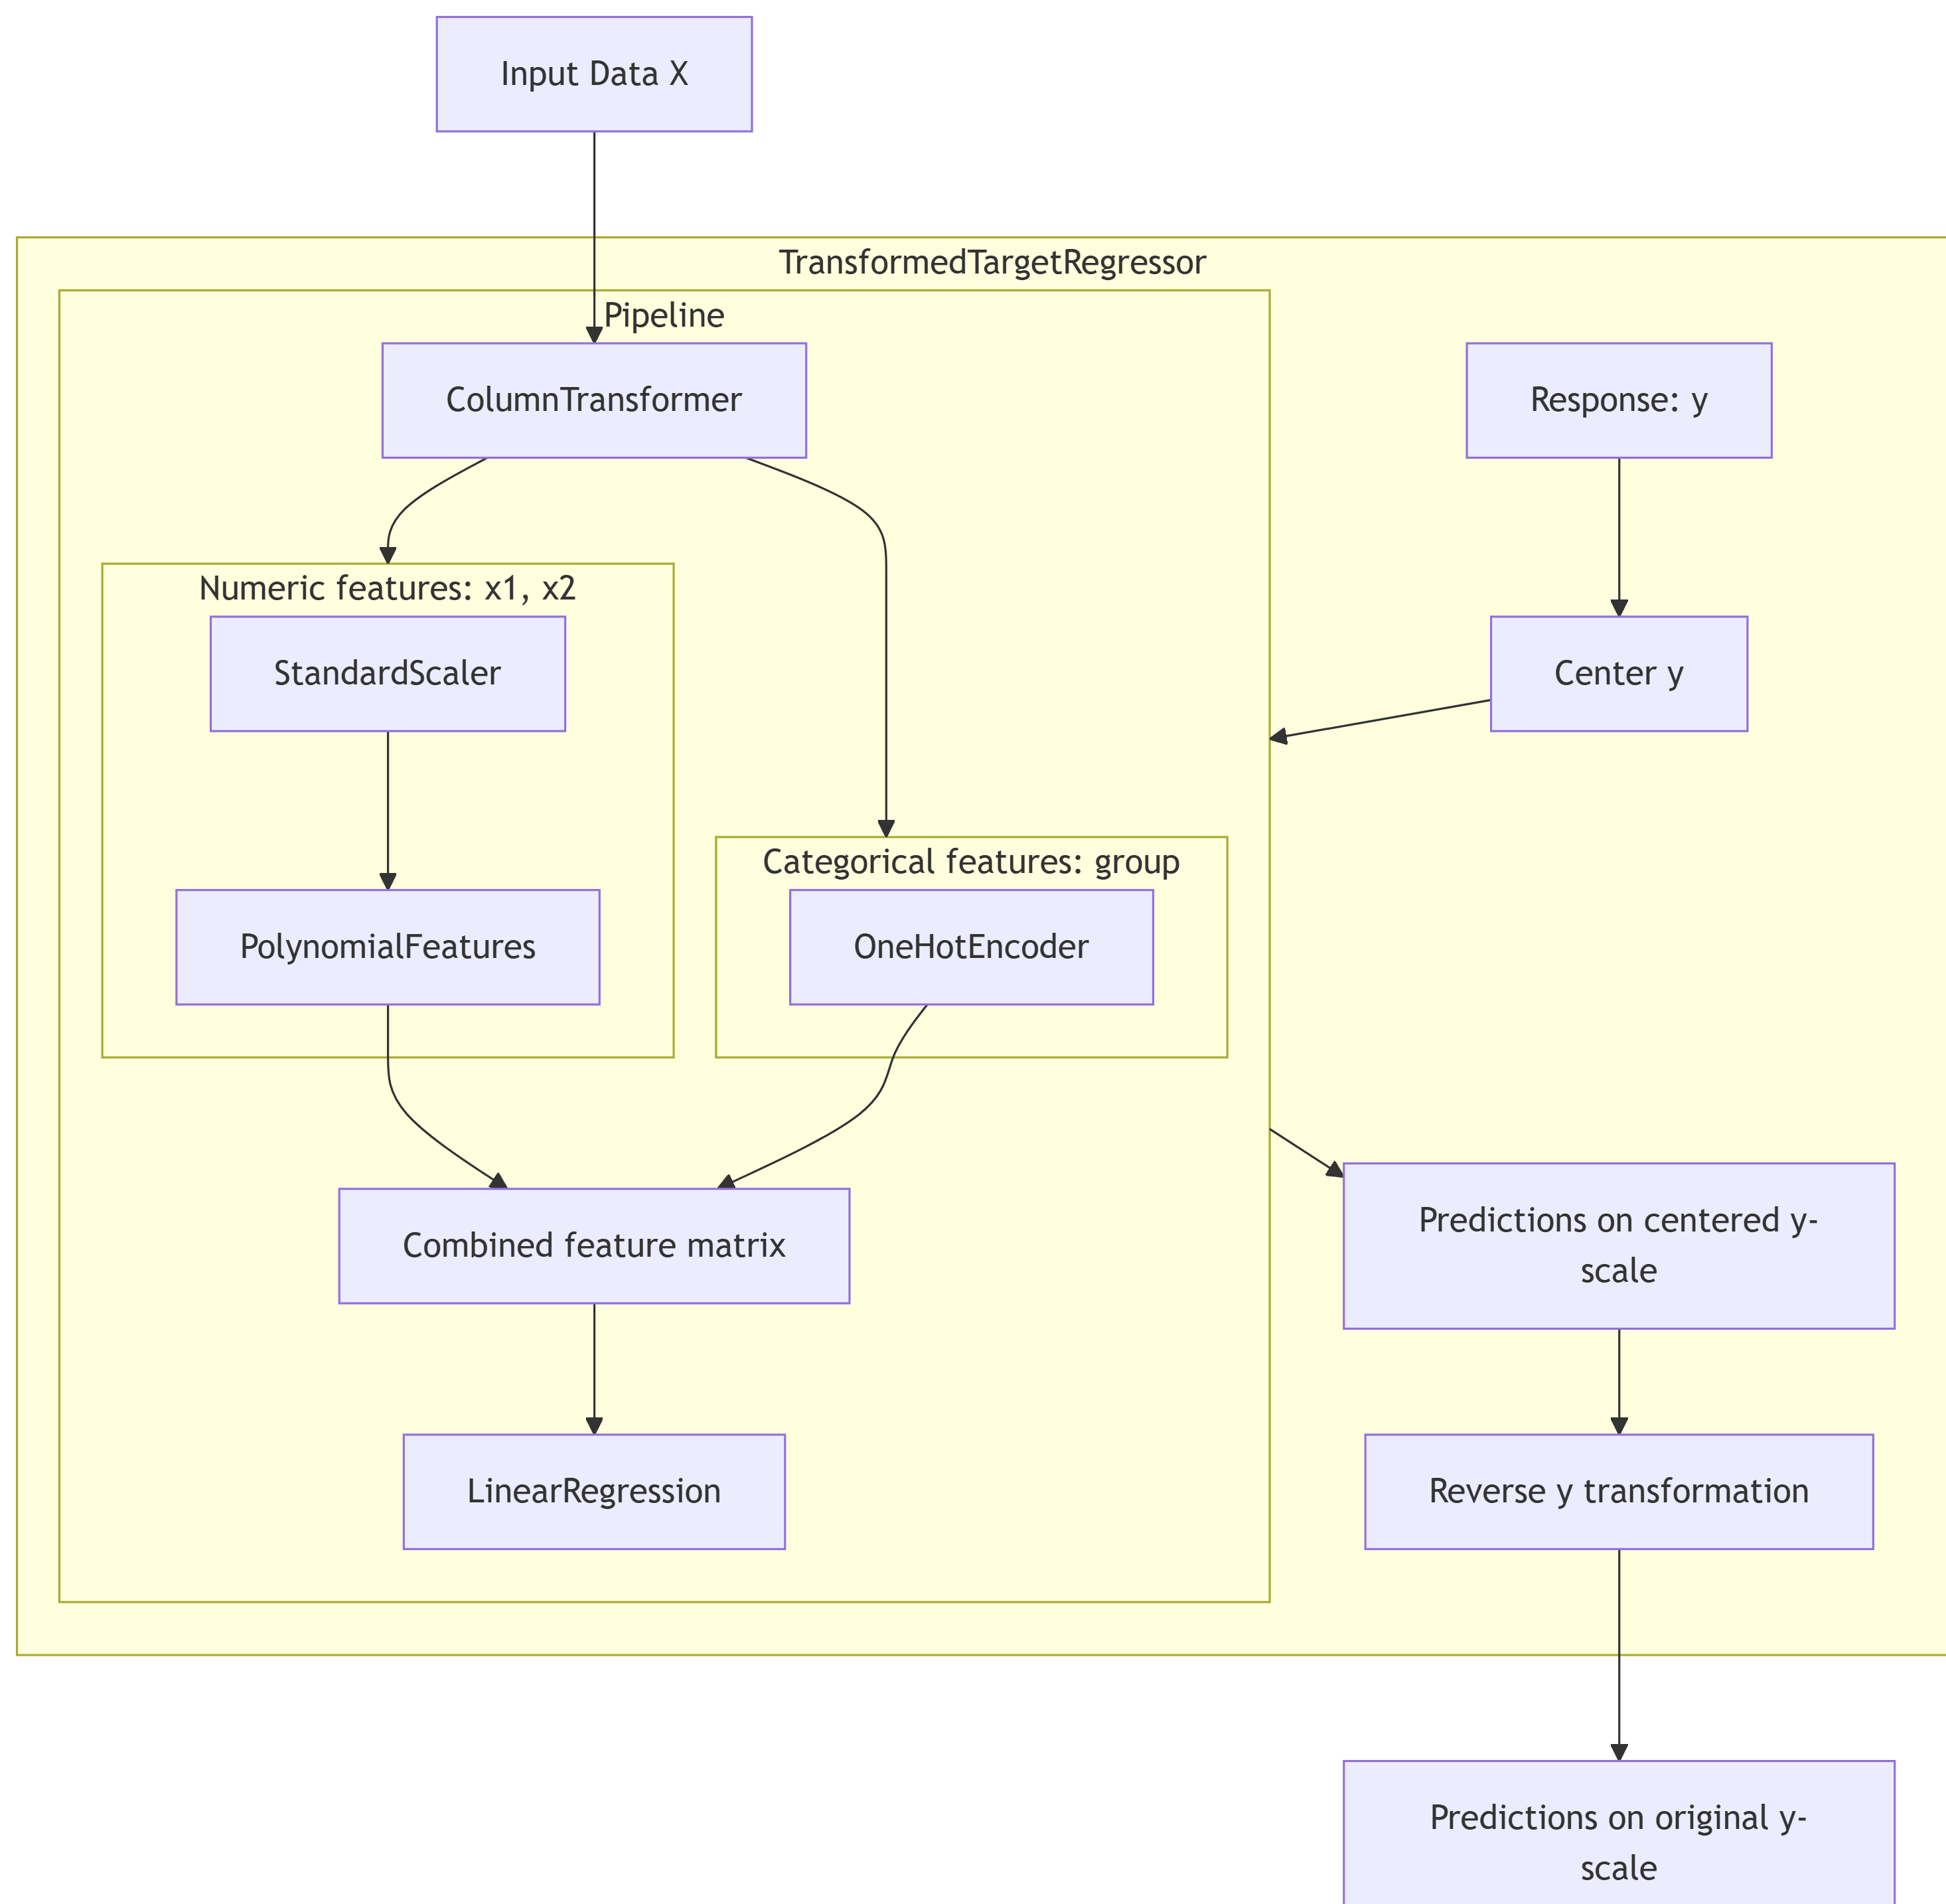
\includegraphics[width=9.76in,height=9.55in]{contents/1/lr_files/figure-latex/mermaid-figure-1.png}

\begin{Shaded}
\begin{Highlighting}[]
\ImportTok{from}\NormalTok{ sklearn.compose }\ImportTok{import}\NormalTok{ ColumnTransformer, TransformedTargetRegressor}
\ImportTok{from}\NormalTok{ sklearn.pipeline }\ImportTok{import}\NormalTok{ Pipeline}
\ImportTok{from}\NormalTok{ sklearn.preprocessing }\ImportTok{import}\NormalTok{ StandardScaler, OneHotEncoder, PolynomialFeatures}
\ImportTok{from}\NormalTok{ sklearn.linear\_model }\ImportTok{import}\NormalTok{ LinearRegression}


\NormalTok{numeric\_features }\OperatorTok{=}\NormalTok{ [}\StringTok{"x1"}\NormalTok{, }\StringTok{"x2"}\NormalTok{]}
\NormalTok{categorical\_features }\OperatorTok{=}\NormalTok{ [}\StringTok{"group"}\NormalTok{]}

\NormalTok{numeric\_pipe }\OperatorTok{=}\NormalTok{ Pipeline(}
\NormalTok{    [}
\NormalTok{        (}\StringTok{"scaler"}\NormalTok{, StandardScaler()),}
\NormalTok{        (}\StringTok{"poly"}\NormalTok{, PolynomialFeatures(degree}\OperatorTok{=}\DecValTok{2}\NormalTok{, include\_bias}\OperatorTok{=}\VariableTok{False}\NormalTok{)),}
\NormalTok{    ]}
\NormalTok{)}

\NormalTok{preprocessor }\OperatorTok{=}\NormalTok{ ColumnTransformer(}
\NormalTok{    [}
\NormalTok{        (}\StringTok{"num"}\NormalTok{, numeric\_pipe, numeric\_features),}
\NormalTok{        (}\StringTok{"cat"}\NormalTok{, OneHotEncoder(drop}\OperatorTok{=}\StringTok{"first"}\NormalTok{), categorical\_features),}
\NormalTok{    ]}
\NormalTok{)}

\NormalTok{pipe }\OperatorTok{=}\NormalTok{ Pipeline(}
\NormalTok{    [}
\NormalTok{        (}\StringTok{"preprocess"}\NormalTok{, preprocessor),}
\NormalTok{        (}\StringTok{"model"}\NormalTok{, LinearRegression()),}
\NormalTok{    ]}
\NormalTok{)}
\NormalTok{model }\OperatorTok{=}\NormalTok{ TransformedTargetRegressor(}
\NormalTok{    regressor}\OperatorTok{=}\NormalTok{pipe,}
\NormalTok{    transformer}\OperatorTok{=}\NormalTok{StandardScaler(with\_std}\OperatorTok{=}\VariableTok{False}\NormalTok{),}
\NormalTok{)}
\end{Highlighting}
\end{Shaded}

The entire \texttt{pipeline} is trained on the training set and then
evaluated on the validation set, where the training and validation sets
are determined by cross-validation.

\begin{Shaded}
\begin{Highlighting}[]
\ImportTok{from}\NormalTok{ sklearn.model\_selection }\ImportTok{import}\NormalTok{ cross\_validate}

\NormalTok{cv\_result }\OperatorTok{=}\NormalTok{ cross\_validate(}
\NormalTok{    model,}
\NormalTok{    X,}
\NormalTok{    y,}
\NormalTok{    cv}\OperatorTok{=}\NormalTok{KFold(}\DecValTok{5}\NormalTok{, shuffle}\OperatorTok{=}\VariableTok{True}\NormalTok{, random\_state}\OperatorTok{=}\DecValTok{1}\NormalTok{),}
\NormalTok{    scoring}\OperatorTok{=}\NormalTok{[}\StringTok{"r2"}\NormalTok{, }\StringTok{"neg\_mean\_squared\_error"}\NormalTok{],}
\NormalTok{)}

\BuiltInTok{print}\NormalTok{(}\SpecialStringTok{f"test R2: }\SpecialCharTok{\{}\NormalTok{cv\_result[}\StringTok{\textquotesingle{}test\_r2\textquotesingle{}}\NormalTok{]}\SpecialCharTok{.}\NormalTok{mean()}\SpecialCharTok{\}}\SpecialStringTok{"}\NormalTok{)}
\BuiltInTok{print}\NormalTok{(}\SpecialStringTok{f"test neg mse: }\SpecialCharTok{\{}\NormalTok{cv\_result[}\StringTok{\textquotesingle{}test\_neg\_mean\_squared\_error\textquotesingle{}}\NormalTok{]}\SpecialCharTok{.}\NormalTok{mean()}\SpecialCharTok{\}}\SpecialStringTok{"}\NormalTok{)}
\end{Highlighting}
\end{Shaded}

\begin{verbatim}
test R2: 0.9158850679164349
test neg mse: -1.0901713224790424
\end{verbatim}

\chapter{Regularization}\label{regularization}

\section{Motivation}\label{motivation}

The OLS estimator is attractive because, under the Gauss--Markov
assumptions, it is BLUE: the best linear unbiased estimator. However,
when some predictors are nearly collinear, the matrix \(X^\top X\)
becomes nearly singular. In that case, the variance of
\(\hat\beta_{\ols}\) can be very large, so the estimated coefficients
may become unstable and unreliable.

This leads to the bias-variance trade-off. By allowing a small amount of
bias, we may substantially reduce the variance and improve predictive
performance. A common way to do this is through regularization.

Two of the most important regularization methods are ridge regression
and lasso. Both methods tend to shrink the coefficients toward zero, so
they are also called shrinkage methods.

\section{Ridge Regression}\label{ridge-regression}

\subsection{OLS estimator review}\label{ols-estimator-review}

Consider a linear model \[
y=X\beta+\varepsilon.
\]

Given the dataset \(X\) and \(y\), the OLS estimator
\(\hat\beta_{\ols}\) finds the coefficient vector \(\beta\) that
minimizes the residual sum of squares \[
\rss(\beta)=\norm{y-X\beta}_2^2.
\] In other words, \[
\hat{\beta}_{\ols} = \arg\min_{\beta}\qty{\norm{y - X\beta}_2^2}.
\] When \(X^\top X\) is invertible, the solution is \[
\hat{\beta}_{\ols} = (X^\top X)^{-1}X^\top y.
\]

\subsection{Ridge estimator}\label{ridge-estimator}

Ridge regression modifies the OLS loss function by adding a quadratic
penalty.

\begin{definition}[Ridge
Regression]\protect\hypertarget{def-}{}\label{def-}

For a response vector \(y \in \mathbb{R}^n\) and a design matrix
\(X \in \mathbb{R}^{n \times p}\), the Ridge estimator
\(\hat{\beta}_{\ridge}\) is defined as: \[
\hat{\beta}_{\ridge} = \arg\min_{\beta} \qty{ \norm{y - X\beta}_2^2 + \lambda \norm{\beta}_2^2 }
\] where

\begin{itemize}
\tightlist
\item
  \(\lambda \ge 0\) is the regularization parameter that controls the
  trade-off between the fit to the data and the penalty on the
  coefficient size.
\item
  \(\norm{\beta}_2^2 = \sum_{j=1}^p \beta_j^2\) is the \(L_2\) norm of
  the coefficient vector
\end{itemize}

\end{definition}

The penalty shrinks the coefficients toward zero. Larger values of
\(\lambda\) produce stronger shrinkage. However, ridge regression does
not perform variable selection, since it rarely sets any coefficient
exactly to zero.

Similar to the OLS estimator, the Ridge estimator can be solved
analytically.

\begin{theorem}[The Closed-Form of Ridge
estimator]\protect\hypertarget{thm-}{}\label{thm-}

The closed-form solution of \(\hat\beta_{\ridge}\) is \[
\hat{\beta}_{\ridge} = (X^\top X + \lambda I)^{-1} X^\top y.
\]

Click for proof.

Consider the ridge regression objective

\[
Q(\beta)
=
(y-X\beta)^\top (y-X\beta) + \lambda \beta^\top \beta, \quad \text{ where }\lambda \ge 0.
\]

We derive the ridge estimator by minimizing \(Q(\beta)\) with respect to
\(\beta\).

First expand the quadratic form:

\[
\begin{aligned}
Q(\beta)
&= (y^\top - \beta^\top X^\top)(y-X\beta) + \lambda \beta^\top \beta \\
&= y^\top y - y^\top X\beta - \beta^\top X^\top y + \beta^\top X^\top X\beta + \lambda \beta^\top \beta .
\end{aligned}
\]

Since \(y^\top X\beta\) is a scalar, it equals its transpose:

\[
y^\top X\beta = \beta^\top X^\top y .
\]

Thus

\[
Q(\beta)
=
y^\top y - 2\beta^\top X^\top y + \beta^\top X^\top X\beta + \lambda \beta^\top \beta .
\]

Combine the last two quadratic terms:

\[
Q(\beta)
=
y^\top y - 2\beta^\top X^\top y + \beta^\top (X^\top X+\lambda I)\beta .
\]

Now differentiate with respect to \(\beta\):

\[
\nabla_\beta Q(\beta)
=
-2X^\top y + 2(X^\top X+\lambda I)\beta .
\]

Set the gradient equal to zero:

\[
-2X^\top y + 2(X^\top X+\lambda I)\beta = 0 .
\]

So

\[
(X^\top X+\lambda I)\beta = X^\top y .
\]

Assuming \(X^\top X+\lambda I\) is invertible, we obtain

\[
\hat{\beta}_{\ridge}
=
(X^\top X+\lambda I)^{-1}X^\top y .
\]

Therefore the ridge estimator is

\[
\hat{\beta}_{\ridge}
=
(X^\top X+\lambda I)^{-1}X^\top y.
\]

\end{theorem}

In this formulation, the term \(\lambda I\) (where \(I\) is the identity
matrix) is added to the cross-product matrix \(X^\top X\) before
inversion. When \(\lambda>0\), this ensures that the matrix is
non-singular and improves its conditioning, even in the presence of
multicollinearity or when \(p > n\).

\subsection{About intercept}\label{about-intercept}

Linear regression models are commonly written in the form

\[
y = X\beta + \varepsilon.
\]

This notation can represent two different model structures depending on
whether an intercept is included.

\begin{itemize}
\tightlist
\item
  Model with intercept:
  \(\beta = [\beta_0,\beta_1,\ldots,\beta_p]^\top\) where \(\beta_0\) is
  the intercept. The design matrix \(X\) contains a leading column of
  ones representing the constant term.
\item
  Model without intercept: \(\beta = [\beta_1,\ldots,\beta_p]^\top\) and
  the design matrix contains only the predictor variables. In this case
  the fitted regression surface is forced to pass through the origin.
\end{itemize}

In most practical applications, models with an intercept are preferred
because they allow the regression function to shift vertically rather
than being constrained to go through the origin.

\begin{tcolorbox}[enhanced jigsaw, arc=.35mm, bottomrule=.15mm, bottomtitle=1mm, breakable, colback=white, colbacktitle=quarto-callout-note-color!10!white, colframe=quarto-callout-note-color-frame, coltitle=black, left=2mm, leftrule=.75mm, opacityback=0, opacitybacktitle=0.6, rightrule=.15mm, title=\textcolor{quarto-callout-note-color}{\faInfo}\hspace{0.5em}{Centering and the No-Intercept Form}, titlerule=0mm, toprule=.15mm, toptitle=1mm]

A model with an intercept can be rewritten as a no-intercept model by
centering both the response and the predictors:

\[
y^c = y - \bar y, 
\qquad
X_j^c = X_j - \bar X_j .
\]

After centering, all variables have mean zero. In ordinary least
squares, the intercept estimate is

\[
\hat\beta_0 = \bar y - \sum_{j=1}^{p}\hat\beta_j \bar X_j .
\]

When the data are centered, this quantity becomes zero automatically. As
a result, fitting a regression without an intercept on centered data
produces the same fitted model as fitting a regression with an intercept
on the original data.

\end{tcolorbox}

For OLS, the intercept formulation and the centered no-intercept
formulation are mathematically equivalent. However, the situation is
slightly different in ridge regression. The ridge estimator introduces
the penalty \[
\lambda \sum_{j=1}^{p} \beta_j^2 ,
\] which is intended to shrink the slope coefficients. In practice the
intercept is not penalized, because penalizing it would shrink the
overall level of the model toward zero and make the result depend on the
arbitrary origin of the response variable.

For this reason ridge regression is usually formulated in the
no-intercept form after centering the data, so that the penalty
naturally applies only to the slope coefficients.

\begin{tcolorbox}[enhanced jigsaw, arc=.35mm, bottomrule=.15mm, bottomtitle=1mm, breakable, colback=white, colbacktitle=quarto-callout-note-color!10!white, colframe=quarto-callout-note-color-frame, coltitle=black, left=2mm, leftrule=.75mm, opacityback=0, opacitybacktitle=0.6, rightrule=.15mm, title=\textcolor{quarto-callout-note-color}{\faInfo}\hspace{0.5em}{Standardization in Practice}, titlerule=0mm, toprule=.15mm, toptitle=1mm]

Because the ridge penalty depends on the sizes of the coefficients,
ridge regression is usually implemented after standardizing the
predictors. This puts the predictors on a common scale, so that the
penalty treats them fairly.

In practice, the predictors are typically standardized, whereas the
response is usually only centered rather than standardized.

For details see Section~\ref{sec-scaling}.

\end{tcolorbox}

\begin{tcolorbox}[enhanced jigsaw, arc=.35mm, bottomrule=.15mm, bottomtitle=1mm, breakable, colback=white, colbacktitle=quarto-callout-note-color!10!white, colframe=quarto-callout-note-color-frame, coltitle=black, left=2mm, leftrule=.75mm, opacityback=0, opacitybacktitle=0.6, rightrule=.15mm, title=\textcolor{quarto-callout-note-color}{\faInfo}\hspace{0.5em}{Implementation in \texttt{scikit-learn}}, titlerule=0mm, toprule=.15mm, toptitle=1mm]

In \texttt{scikit-learn}, ridge and lasso regression automatically
center the data internally when fitting the model (while leaving the
final predictions on the original scale). The intercept is therefore
handled separately and excluded from the penalty.

Because of this internal preprocessing, users typically do not need to
manually center the response when using \texttt{Ridge} or
\texttt{Lasso}. However, it is still common to standardize the
predictors explicitly using tools such as \texttt{StandardScaler},
especially when building modeling pipelines.

\end{tcolorbox}

\subsection{Alternative Formulation}\label{alternative-formulation}

By the theory of Lagrange multipliers, ridge regression can also be
written in a constrained optimization form:

\[
\hat{\beta}_{\ridge}
=
\arg\min_{\beta} \norm{y-X\beta}_2^2
\quad
\text{subject to}
\quad
\norm{\beta}_2^2 \le s .
\]

Here \(s \ge 0\) controls the size of the coefficient vector and is
directly related to the penalty parameter \(\lambda\). The two
parameters have an inverse relationship:

\begin{itemize}
\tightlist
\item
  Large \(s\) corresponds to small \(\lambda\). The constraint is weak,
  and \(\beta\) approaches the OLS estimator.
\item
  Small \(s\) corresponds to large \(\lambda\). The constraint is
  strong, and \(\beta\) shrinks toward \(0\).
\end{itemize}

This formulation highlights that ridge regression limits the magnitude
of the coefficient vector rather than directly penalizing prediction
error. We will later use this interpretation to explain the difference
between ridge regression and lasso.

\begin{tcolorbox}[enhanced jigsaw, arc=.35mm, bottomrule=.15mm, bottomtitle=1mm, breakable, colback=white, colbacktitle=quarto-callout-note-color!10!white, colframe=quarto-callout-note-color-frame, coltitle=black, left=2mm, leftrule=.75mm, opacityback=0, opacitybacktitle=0.6, rightrule=.15mm, title=\textcolor{quarto-callout-note-color}{\faInfo}\hspace{0.5em}{The Constrained Optimization Problem}, titlerule=0mm, toprule=.15mm, toptitle=1mm]

Ridge regression can be formulated as a constrained optimization
problem, where we minimize RSS subject to a constraint \(s\) on the
squared \(L_2\) norm of the coefficients: \[
\min_{\beta} \norm{y - X\beta}_2^2 \quad \text{subject to} \quad \norm{\beta}_2^2 \le s.
\]

To solve this, we define the Lagrangian function
\(\mathcal{L}(\beta, \lambda)\): \[
\mathcal{L}(\beta, \lambda) = \norm{y - X\beta}_2^2 + \lambda (\norm{\beta}_2^2 - s)
\] where \(\lambda \ge 0\) is the Lagrange multiplier. Taking the
partial derivative with respect to \(\beta\) and setting it to zero
gives: \[
\frac{\partial \mathcal{L}}{\partial \beta} = -2X^\top(y - X\beta) + 2\lambda\beta = 0
\] Rearranging the terms yields the standard ridge estimator: \[
(X^\top X + \lambda I)\beta = X^\top y \implies \hat{\beta}_{\text{ridge}} = (X^\top X + \lambda I)^{-1} X^\top y.
\] This shows that for every \(\lambda > 0\), there exists an equivalent
constrained problem with some constraint \(s\).

\end{tcolorbox}

\begin{tcolorbox}[enhanced jigsaw, arc=.35mm, bottomrule=.15mm, bottomtitle=1mm, breakable, colback=white, colbacktitle=quarto-callout-note-color!10!white, colframe=quarto-callout-note-color-frame, coltitle=black, left=2mm, leftrule=.75mm, opacityback=0, opacitybacktitle=0.6, rightrule=.15mm, title=\textcolor{quarto-callout-note-color}{\faInfo}\hspace{0.5em}{Relation Between \(\lambda\) and \(s\)}, titlerule=0mm, toprule=.15mm, toptitle=1mm]

The connection between the penalty parameter \(\lambda\) and the
constraint \(s\) can be understood through the constrained formulation

\[
\min_\beta \norm{y-X\beta}_2^2
\quad
\text{subject to}
\quad
\norm{\beta}_2^2 \le s.
\]

There are two possible scenarios:

\begin{itemize}
\tightlist
\item
  Non-binding constraint: If the OLS solution already satisfies
  \(\norm{\hat{\beta}_{\text{ols}}}_2^2 \le s\), then the OLS solution
  remains optimal for the constrained problem. Therefore,
  \(\hat{\beta}_{\text{ridge}}=\hat{\beta}_{\text{ols}}\). The
  constraint has no effect, so the corresponding penalized formulation
  uses \(\lambda = 0\).
\item
  Binding constraint: If \(\norm{\hat{\beta}_{\text{ols}}}_2^2 > s\),
  then the OLS solution lies outside the constraint region. The
  constrained optimum must therefore lie on the boundary
  \(\norm{\hat{\beta}_{\text{ridge}}}_2^2 = s\). Consequently, the
  corresponding penalized formulation requires \(\lambda > 0\).
\end{itemize}

Therefore, when \(\lambda>0\), the parameters \(\lambda\) and \(s\) are
related through \(\norm{(X^\top X+\lambda I)^{-1}X^\top y}_2^2=s\).

The parameter \(\lambda\) can be viewed as the ``price'' paid for
enforcing the constraint. As \(s\) decreases, the corresponding value of
\(\lambda\) increases, producing greater shrinkage toward the origin.
Since the norm of the ridge estimator decreases as \(\lambda\)
increases, smaller values of \(s\) correspond to larger values of
\(\lambda\).

Consequently, for every \(s < \norm{\hat{\beta}_{\text{ols}}}_2^2\),
there exists a unique \(\lambda>0\) such that
\(\norm{\hat{\beta}_{\text{ridge}}}_2^2=s\).

This relationship is consistent with the Karush--Kuhn--Tucker (KKT)
complementary slackness condition in optimization theory,

\[
\lambda\left(\norm{\beta}_2^2-s\right)=0.
\]

\end{tcolorbox}

\subsection{SVD and Tikhonov
Regularization}\label{svd-and-tikhonov-regularization}

Recall the OLS estimator

\[
\hat{\beta}_{\ols} = (X^\top X)^{-1}X^\top y .
\]

Let the singular value decomposition (SVD) of \(X\) be

\[
X = UDV^\top ,
\]

where

\begin{itemize}
\tightlist
\item
  \(U\) is an \(n \times n\) orthogonal matrix,
\item
  \(V\) is a \(p \times p\) orthogonal matrix,
\item
  \(D\) is an \(n \times p\) diagonal matrix whose nonzero entries
  \(d_1,\ldots,d_r\) are the singular values of \(X\).
\end{itemize}

\begin{tcolorbox}[enhanced jigsaw, arc=.35mm, bottomrule=.15mm, bottomtitle=1mm, breakable, colback=white, colbacktitle=quarto-callout-note-color!10!white, colframe=quarto-callout-note-color-frame, coltitle=black, left=2mm, leftrule=.75mm, opacityback=0, opacitybacktitle=0.6, rightrule=.15mm, title=\textcolor{quarto-callout-note-color}{\faInfo}\hspace{0.5em}{Thin SVD}, titlerule=0mm, toprule=.15mm, toptitle=1mm]

Let \(X = UDV^\top\) be the (full) singular value decomposition of
\(X\), and let \(r=\operatorname{rank}(X)\). If \(r<\min(n,p)\), then
\(D^\top D\) contains zero eigenvalues and is therefore singular.

In statistical learning, we are usually interested in expressions
involving \(D^{-1}\) or \((D^\top D)^{-1}\) rather than the complete
orthogonal basis structure of \(U\) and \(V\). Therefore, it is often
more convenient to work with the \textbf{thin (reduced) SVD}
\(X = U_r D_r V_r^\top\), where \(U_r\) and \(V_r\) are obtained by
removing the columns corresponding to zero singular values, and \(D_r\)
is obtained by deleting the associated zero rows and columns of \(D\).
Consequently, \(D_r=\operatorname{diag}(\sigma_1,\ldots,\sigma_r)\) is
square and invertible.

By a slight abuse of notation, statistical learning texts often write
\(X = UDV^\top\) while actually referring to the thin SVD. We follow
this convention throughout this section. Unless otherwise stated, all
SVDs appearing below should be interpreted as thin SVDs.

\end{tcolorbox}

Using the SVD,

\[
X^\top X = V D^\top D V^\top .
\]

Since \(D^\top D = \mathrm{diag}(d_1^2,\ldots,d_r^2)\), the eigenvalues
of \(X^\top X\) are \(d_i^2\).\\
Hence the OLS estimator can be written as

\[
\hat{\beta}_{\ols}
=
V(D^\top D)^{-1}D^\top U^\top y .
\]

Since \(D^\top D=\mathrm{diag}(d_1^2,\ldots,d_r^2)\), we have

\[
(D^\top D)^{-1}=\mathrm{diag}\qty(\frac{1}{d_1^2},\ldots,\frac{1}{d_r^2}).
\] Let \(u_i\) and \(v_i\) denote the columns of \(U\) and \(V\). Then
the estimator can be written as

\[
\hat{\beta}_{\ols}
=
\sum_{i=1}^{r}
\frac{1}{d_i}\, v_i\, u_i^\top y .
\]

If some singular values \(d_i\) are very small, the factors \(1/d_i\)
become very large, which leads to unstable coefficient estimates.
Therefore this expression reveals the instability of OLS.

Now turn to Ridge regression. We replace the OLS estimator with

\[
\hat{\beta}_{\text{ridge}}
=
(X^\top X+\lambda I)^{-1}X^\top y .
\]

Substituting the SVD gives

\[
\hat{\beta}_{\text{ridge}}
=
V(D^\top D+\lambda I)^{-1}D^\top U^\top y .
\]

Because \(D^\top D\) is diagonal, the estimator can be written
componentwise as

\[
\hat{\beta}_{\text{ridge}}
=
\sum_{i=1}^{r}
\frac{d_i}{d_i^2+\lambda}
v_i\,u_i^\top y .
\]

This representation shows that ridge regression applies a shrinkage
factor

\[
\frac{d_i^2}{d_i^2+\lambda}
\]

to each principal component direction.

\begin{itemize}
\tightlist
\item
  When \(d_i\) is large, the factor is close to \(1\), so the component
  is almost unchanged.
\item
  When \(d_i\) is small, the factor becomes small, shrinking the
  unstable directions.
\end{itemize}

Thus ridge regression stabilizes the estimator by shrinking the
contributions of directions associated with small singular values.

\begin{tcolorbox}[enhanced jigsaw, arc=.35mm, bottomrule=.15mm, bottomtitle=1mm, breakable, colback=white, colbacktitle=quarto-callout-tip-color!10!white, colframe=quarto-callout-tip-color-frame, coltitle=black, left=2mm, leftrule=.75mm, opacityback=0, opacitybacktitle=0.6, rightrule=.15mm, title=\textcolor{quarto-callout-tip-color}{\faLightbulb}\hspace{0.5em}{Tikhonov regularization}, titlerule=0mm, toprule=.15mm, toptitle=1mm]

Tikhonov regularization is a method used to solve ill-posed problems and
handle multicollinearity by adding a penalty term,
\(\alpha\norm{L\beta}_2^2\). When the Tikhonov matrix \(L\) is the
identity matrix \(I\), it simplifies to ridge regression. Therefore,
ridge regression is a special case of Tikhonov regularization {[}2,
3{]}.

\end{tcolorbox}

\subsection{Bias-Variance Tradeoff}\label{bias-variance-tradeoff}

One of the main motivations for regularization methods is the
bias-variance tradeoff. A more flexible model can fit the training data
very well, but it may also be highly sensitive to random noise in the
sample. In contrast, a more constrained model is usually more stable,
but may systematically miss part of the true signal.

This tradeoff can be described mathematically through a decomposition of
the expected prediction error.

Suppose the true model is \[
Y=f(x)+\varepsilon,\quad\Exp(\varepsilon)=0,\quad \Var(\varepsilon)=\sigma^2.
\]

Let \(\hat f(x)\) be an estimator of \(f(x)\) constructed from a
training sample. Since the training sample is random, \(\hat f(x)\) is
also random. We study the expected prediction error at a fixed point
\(x\): \[
\Exp\qty[(Y-\hat f(x))^2].
\]

Here, the expectation is taken over both the randomness in the training
data and the randomness in the new response \(Y\).

\begin{definition}[Bias and
Variance]\protect\hypertarget{def-}{}\label{def-}

~

\begin{itemize}
\tightlist
\item
  \(\operatorname{Bias}(\hat f(x))=\Exp[\hat f(x)]-f(x)\).
\item
  \(\Var(\hat f(x))=\Exp\qty[\qty(\hat f(x)-\Exp[\hat f(x)])^2]\).
\end{itemize}

\end{definition}

\begin{theorem}[Bias-Variance
Decomposition]\protect\hypertarget{thm-}{}\label{thm-}

\[
\Exp\qty[(Y-\hat f(x))^2]
=
\operatorname{Bias}(\hat f(x))^2+\operatorname{Var}(\hat f(x))+\sigma^2.
\]

Click to expand.

Since \(Y=f(x)+\varepsilon\), \[
\begin{split}
\Exp\qty[(Y-\hat f(x))^2]&=\Exp\qty[(f(x)+\varepsilon-\hat f(x))^2]\\
&=\Exp\qty[(f(x)-\hat f(x))^2+2\varepsilon(f(x)-\hat f(x))+\varepsilon^2]\\
&=\Exp\qty[(f(x)-\hat f(x))^2]+2\Exp\qty[\varepsilon(f(x)-\hat f(x))]+\Exp(\varepsilon^2).
\end{split}
\]

Since the new noise \(\varepsilon\) is independent of the training data
and has mean \(0\), \[
\Exp\qty[\varepsilon(f(x)-\hat f(x))]=0.
\] Also, \[
\Exp(\varepsilon^2)=\Var(\varepsilon)=\sigma^2.
\]

Therefore, \[
\Exp\qty[(Y-\hat f(x))^2]
=
\Exp\qty[(f(x)-\hat f(x))^2]+\sigma^2.
\]

Thus the prediction error is the sum of:

\begin{itemize}
\tightlist
\item
  the estimation error \(\mathbb{E}[(f(x)-\hat f(x))^2]\),
\item
  the irreducible error \(\sigma^2\).
\end{itemize}

Now we further decompose \[
\Exp\qty[(f(x)-\hat f(x))^2].
\]

Let \[
m(x)=\Exp[\hat f(x)],
\] where the expectation is taken over the randomness in the training
sample. Then \[
f(x)-\hat f(x)=\qty(f(x)-m(x))+\qty(m(x)-\hat f(x)).
\]

Squaring, \[
(f(x)-\hat f(x))^2
=
(f(x)-m(x))^2
+
(m(x)-\hat f(x))^2
+
2\qty(f(x)-m(x))\qty(m(x)-\hat f(x)).
\]

Taking expectation, \[
\Exp\qty[(f(x)-\hat f(x))^2]
=
(f(x)-m(x))^2
+
\Exp\qty[(m(x)-\hat f(x))^2]
+
2\qty(f(x)-m(x))\Exp[m(x)-\hat f(x)].
\]

But \[
\Exp[m(x)-\hat f(x)]
=
m(x)-\Exp[\hat f(x)]
=
0.
\]

So the cross term vanishes, and we obtain \[
\Exp\qty[(f(x)-\hat f(x))^2]
=
\qty(f(x)-\Exp[\hat f(x)])^2
+
\Exp\qty[\qty(\hat f(x)-\Exp[\hat f(x)])^2].
\]

The first term is the squared bias: \[
\operatorname{Bias}(\hat f(x))^2
=
\qty(\Exp[\hat f(x)]-f(x))^2.
\]

The second term is the variance: \[
\Var(\hat f(x))
=
\Exp\qty[\qty(\hat f(x)-\Exp[\hat f(x)])^2].
\]

Therefore, \[
\Exp\qty[(f(x)-\hat f(x))^2]
=
\operatorname{Bias}(\hat f(x))^2+\Var(\hat f(x)).
\]

Combining this with the earlier decomposition gives \[
\Exp\qty[(Y-\hat f(x))^2]
=
\operatorname{Bias}(\hat f(x))^2+\operatorname{Var}(\hat f(x))+\sigma^2.
\]

\end{theorem}

This formula shows that the expected prediction error has three parts:

\begin{itemize}
\tightlist
\item
  Squared bias: error caused by systematic deviation of the estimator
  from the truth.
\item
  Variance: error caused by sensitivity of the estimator to the
  particular training sample.
\item
  Irreducible error: the noise level \(\sigma^2\), which cannot be
  removed by any method.
\end{itemize}

A very flexible model often has small bias but large variance. A more
constrained model often has larger bias but smaller variance. The goal
of regularization is not necessarily to minimize bias or variance alone,
but to balance them so that the total prediction error is as small as
possible.

\begin{tcolorbox}[enhanced jigsaw, arc=.35mm, bottomrule=.15mm, bottomtitle=1mm, breakable, colback=white, colbacktitle=quarto-callout-note-color!10!white, colframe=quarto-callout-note-color-frame, coltitle=black, left=2mm, leftrule=.75mm, opacityback=0, opacitybacktitle=0.6, rightrule=.15mm, title=\textcolor{quarto-callout-note-color}{\faInfo}\hspace{0.5em}{Note}, titlerule=0mm, toprule=.15mm, toptitle=1mm]

Ordinary least squares is often unbiased, but its variance can be very
large when predictors are highly correlated or when the model is too
flexible. Ridge and lasso (which will be discussed later) introduce bias
by shrinking the coefficients toward \(0\), but this often substantially
reduces variance.

As a result, although ridge or lasso may fit the training data less
perfectly than OLS, they can achieve better prediction performance on
new data. This is the central idea behind the bias-variance tradeoff and
one of the main reasons regularization methods are useful in statistical
learning.

\end{tcolorbox}

\section{Ridge Regression in Python}\label{ridge-regression-in-python}

We use the following simulated dataset to demonstrate ridge regression.

The covariance matrix has a very high correlation, so the two predictors
\(x_1\) and \(x_2\) are highly correlated.

\begin{Shaded}
\begin{Highlighting}[]
\ImportTok{import}\NormalTok{ numpy }\ImportTok{as}\NormalTok{ np}

\NormalTok{rng }\OperatorTok{=}\NormalTok{ np.random.default\_rng(}\DecValTok{2}\NormalTok{)}
\NormalTok{n }\OperatorTok{=} \DecValTok{30}

\NormalTok{Sigma }\OperatorTok{=}\NormalTok{ np.array([[}\DecValTok{1}\NormalTok{, }\FloatTok{0.99}\NormalTok{], [}\FloatTok{0.99}\NormalTok{, }\DecValTok{1}\NormalTok{]])}
\NormalTok{mean }\OperatorTok{=}\NormalTok{ np.array([}\DecValTok{0}\NormalTok{, }\DecValTok{0}\NormalTok{])}

\NormalTok{X }\OperatorTok{=}\NormalTok{ rng.multivariate\_normal(mean, Sigma, size}\OperatorTok{=}\NormalTok{n)}
\NormalTok{y }\OperatorTok{=}\NormalTok{ rng.normal(loc}\OperatorTok{=}\NormalTok{X[:, }\DecValTok{0}\NormalTok{] }\OperatorTok{+}\NormalTok{ X[:, }\DecValTok{1}\NormalTok{], scale}\OperatorTok{=}\DecValTok{1}\NormalTok{)}
\end{Highlighting}
\end{Shaded}

The data set is generated from a model with
\(\Exp(y\mid x_1,x_2)=x_1+x_2\). Therefore the true coefficients are
\(\beta_1=\beta_2=1\).

\subsection{Ridge estimator}\label{ridge-estimator-1}

We use \texttt{Ridge} from \texttt{sklearn.linear\_model} to fit a ridge
regression model. Its API is very similar to that of OLS. The argument
\texttt{alpha} is the regularization parameter \(\lambda\).

For simplicity, we use a no-intercept model, so we set
\texttt{fit\_intercept=False}.

\begin{Shaded}
\begin{Highlighting}[]
\ImportTok{from}\NormalTok{ sklearn.linear\_model }\ImportTok{import}\NormalTok{ Ridge}

\NormalTok{ridge }\OperatorTok{=}\NormalTok{ Ridge(alpha}\OperatorTok{=}\DecValTok{5}\NormalTok{, fit\_intercept}\OperatorTok{=}\VariableTok{False}\NormalTok{).fit(X, y)}
\BuiltInTok{print}\NormalTok{(}\SpecialStringTok{f"Ridge beta = }\SpecialCharTok{\{}\NormalTok{ridge}\SpecialCharTok{.}\NormalTok{coef\_}\SpecialCharTok{\}}\SpecialStringTok{"}\NormalTok{)}
\end{Highlighting}
\end{Shaded}

\begin{verbatim}
Ridge beta = [0.85769874 0.84964704]
\end{verbatim}

For comparison, we also fit the OLS estimator.

\begin{Shaded}
\begin{Highlighting}[]
\ImportTok{from}\NormalTok{ sklearn.linear\_model }\ImportTok{import}\NormalTok{ LinearRegression}

\NormalTok{ols }\OperatorTok{=}\NormalTok{ LinearRegression(fit\_intercept}\OperatorTok{=}\VariableTok{False}\NormalTok{).fit(X, y)}
\BuiltInTok{print}\NormalTok{(}\SpecialStringTok{f"OLS beta = }\SpecialCharTok{\{}\NormalTok{ols}\SpecialCharTok{.}\NormalTok{coef\_}\SpecialCharTok{\}}\SpecialStringTok{"}\NormalTok{)}
\end{Highlighting}
\end{Shaded}

\begin{verbatim}
OLS beta = [0.99640827 0.85969191]
\end{verbatim}

In this example, you may notice two things:

\begin{itemize}
\tightlist
\item
  The ridge coefficients are smaller in magnitude than the OLS
  coefficients.
\item
  The OLS coefficients may happen to be closer to the true values in
  this single sample.
\end{itemize}

The second point is due to randomness in the simulated data. To see the
general pattern, we repeat the simulation many times.

\begin{Shaded}
\begin{Highlighting}[]
\ImportTok{import}\NormalTok{ pandas }\ImportTok{as}\NormalTok{ pd}

\NormalTok{res }\OperatorTok{=}\NormalTok{ []}
\ControlFlowTok{for}\NormalTok{ \_ }\KeywordTok{in} \BuiltInTok{range}\NormalTok{(}\DecValTok{100}\NormalTok{):}
\NormalTok{    X }\OperatorTok{=}\NormalTok{ rng.multivariate\_normal(mean, Sigma, size}\OperatorTok{=}\NormalTok{n)}
\NormalTok{    y }\OperatorTok{=}\NormalTok{ rng.normal(loc}\OperatorTok{=}\NormalTok{X[:, }\DecValTok{0}\NormalTok{] }\OperatorTok{+}\NormalTok{ X[:, }\DecValTok{1}\NormalTok{], scale}\OperatorTok{=}\DecValTok{1}\NormalTok{)}
\NormalTok{    ols }\OperatorTok{=}\NormalTok{ LinearRegression(fit\_intercept}\OperatorTok{=}\VariableTok{False}\NormalTok{).fit(X, y)}
\NormalTok{    ridge }\OperatorTok{=}\NormalTok{ Ridge(alpha}\OperatorTok{=}\DecValTok{5}\NormalTok{, fit\_intercept}\OperatorTok{=}\VariableTok{False}\NormalTok{).fit(X, y)}
\NormalTok{    res.append(}
\NormalTok{        \{}
            \StringTok{"ols\_b1"}\NormalTok{: ols.coef\_[}\DecValTok{0}\NormalTok{],}
            \StringTok{"ols\_b2"}\NormalTok{: ols.coef\_[}\DecValTok{1}\NormalTok{],}
            \StringTok{"ridge\_b1"}\NormalTok{: ridge.coef\_[}\DecValTok{0}\NormalTok{],}
            \StringTok{"ridge\_b2"}\NormalTok{: ridge.coef\_[}\DecValTok{1}\NormalTok{],}
\NormalTok{        \}}
\NormalTok{    )}
\NormalTok{res }\OperatorTok{=}\NormalTok{ pd.DataFrame(res)}
\end{Highlighting}
\end{Shaded}

The first five results are shown below. We can see that the OLS
estimates vary substantially from sample to sample.

\begin{Shaded}
\begin{Highlighting}[]
\NormalTok{res.head(}\DecValTok{5}\NormalTok{)}
\end{Highlighting}
\end{Shaded}

{\def\LTcaptype{none} % do not increment counter
\begin{longtable}[]{@{}lllll@{}}
\toprule\noalign{}
& ols\_b1 & ols\_b2 & ridge\_b1 & ridge\_b2 \\
\midrule\noalign{}
\endhead
\bottomrule\noalign{}
\endlastfoot
0 & 1.642753 & 0.343583 & 0.908249 & 0.883823 \\
1 & 1.105216 & 0.774858 & 0.885627 & 0.858433 \\
2 & -0.978268 & 3.091366 & 0.797745 & 1.092525 \\
3 & 1.301118 & 0.325411 & 0.781313 & 0.728571 \\
4 & -0.626684 & 2.741871 & 0.926826 & 1.008491 \\
\end{longtable}
}

This becomes even clearer in the boxplot below, which shows that the
ridge estimator has much smaller variance than the OLS estimator.

\begin{Shaded}
\begin{Highlighting}[]
\ImportTok{import}\NormalTok{ seaborn }\ImportTok{as}\NormalTok{ sns}
\NormalTok{sns.boxplot(res)}
\end{Highlighting}
\end{Shaded}

\pandocbounded{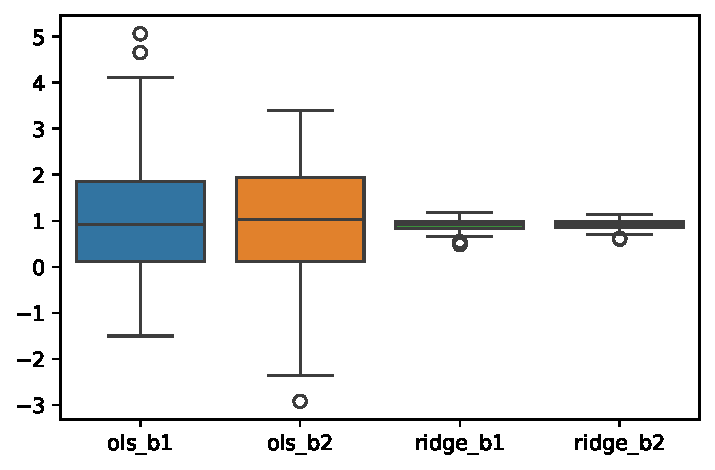
\includegraphics[keepaspectratio]{contents/1/shrinkage_files/figure-pdf/cell-7-output-1.pdf}}

\subsection{Contour map}\label{contour-map}

The variance of both \(\hat{\beta}_1\) and \(\hat{\beta}_2\) is quite
large under OLS. This is because the variance of
\(\widehat{\boldsymbol{\beta}}\) is
\(\sigma^2(\mathbf{X}^\top\mathbf{X})^{-1}\). Since the columns of
\(\mathbf{X}\) are highly correlated, the smallest eigenvalue of
\(\mathbf{X}^\top\mathbf{X}\) is close to zero, making the largest
eigenvalue of \((\mathbf{X}^\top\mathbf{X})^{-1}\) very large.

To see things in more details, we first build the RSS function. For each
\(\beta_1\) and \(\beta_2\) in the range, we form a model
\(\hat y_{\beta}=\beta_1x_1+\beta_2x_2\) and use it to compute
\(\rss = \sum (y-\hat y)^2\).

\begin{Shaded}
\begin{Highlighting}[]
\NormalTok{beta1\_vals }\OperatorTok{=}\NormalTok{ np.linspace(}\OperatorTok{{-}}\DecValTok{1}\NormalTok{, }\DecValTok{3}\NormalTok{, }\DecValTok{200}\NormalTok{)}
\NormalTok{beta2\_vals }\OperatorTok{=}\NormalTok{ np.linspace(}\OperatorTok{{-}}\DecValTok{1}\NormalTok{, }\DecValTok{3}\NormalTok{, }\DecValTok{200}\NormalTok{)}
\NormalTok{B1, B2 }\OperatorTok{=}\NormalTok{ np.meshgrid(beta1\_vals, beta2\_vals)}

\NormalTok{betas }\OperatorTok{=}\NormalTok{ np.column\_stack([B1.ravel(), B2.ravel()])}
\NormalTok{preds }\OperatorTok{=}\NormalTok{ X }\OperatorTok{@}\NormalTok{ betas.T}
\NormalTok{rss\_term }\OperatorTok{=}\NormalTok{ np.}\BuiltInTok{sum}\NormalTok{((y.reshape(}\OperatorTok{{-}}\DecValTok{1}\NormalTok{, }\DecValTok{1}\NormalTok{) }\OperatorTok{{-}}\NormalTok{ preds) }\OperatorTok{**} \DecValTok{2}\NormalTok{, axis}\OperatorTok{=}\DecValTok{0}\NormalTok{)}
\NormalTok{rss\_value0 }\OperatorTok{=}\NormalTok{ rss\_term.reshape(B1.shape)}
\end{Highlighting}
\end{Shaded}

We then construct the contour map for the \(\rss\) surface, plotting the
isolines that correspond to the 1\%, 2.5\%, 5\%, 20\%, 50\%, and 75\%
quantiles of the distribution. The ture coefficient
\((\beta_1=1,\beta_2=1)\) is displayed as the red dot, as well as the
estimated \(\beta\) as a blue square in the countour map.

\begin{Shaded}
\begin{Highlighting}[]
\ImportTok{import}\NormalTok{ matplotlib.pyplot }\ImportTok{as}\NormalTok{ plt}

\NormalTok{quant\_levels }\OperatorTok{=}\NormalTok{ np.quantile(rss\_value0, [}\FloatTok{0.01}\NormalTok{, }\FloatTok{0.025}\NormalTok{, }\FloatTok{0.05}\NormalTok{, }\FloatTok{0.2}\NormalTok{, }\FloatTok{0.5}\NormalTok{, }\FloatTok{0.75}\NormalTok{])}

\NormalTok{fig, ax }\OperatorTok{=}\NormalTok{ plt.subplots(figsize}\OperatorTok{=}\NormalTok{(}\DecValTok{6}\NormalTok{, }\DecValTok{5}\NormalTok{))}
\NormalTok{cs }\OperatorTok{=}\NormalTok{ ax.contour(B1, B2, rss\_value0, levels}\OperatorTok{=}\NormalTok{quant\_levels, colors}\OperatorTok{=}\StringTok{"steelblue"}\NormalTok{)}
\NormalTok{ax.clabel(cs, inline}\OperatorTok{=}\VariableTok{True}\NormalTok{, fontsize}\OperatorTok{=}\DecValTok{8}\NormalTok{, fmt}\OperatorTok{=}\StringTok{"\%.0f"}\NormalTok{)}

\NormalTok{ax.plot(}\DecValTok{1}\NormalTok{, }\DecValTok{1}\NormalTok{, }\StringTok{"ro"}\NormalTok{, markersize}\OperatorTok{=}\DecValTok{10}\NormalTok{, label}\OperatorTok{=}\StringTok{"True (1, 1)"}\NormalTok{)}
\NormalTok{ax.plot(ols.coef\_[}\DecValTok{0}\NormalTok{], ols.coef\_[}\DecValTok{1}\NormalTok{], }\StringTok{"bs"}\NormalTok{, markersize}\OperatorTok{=}\DecValTok{10}\NormalTok{, label}\OperatorTok{=}\StringTok{"OLS estimate"}\NormalTok{)}

\NormalTok{ax.set\_xlabel(}\VerbatimStringTok{r"}\DecValTok{$\textbackslash{}b}\VerbatimStringTok{eta\_1}\DecValTok{$}\VerbatimStringTok{"}\NormalTok{)}
\NormalTok{ax.set\_ylabel(}\VerbatimStringTok{r"}\DecValTok{$\textbackslash{}b}\VerbatimStringTok{eta\_2}\DecValTok{$}\VerbatimStringTok{"}\NormalTok{)}
\NormalTok{ax.set\_title(}\StringTok{"OLS Objective Function Contours"}\NormalTok{)}
\NormalTok{ax.legend()}
\NormalTok{plt.tight\_layout()}
\end{Highlighting}
\end{Shaded}

\pandocbounded{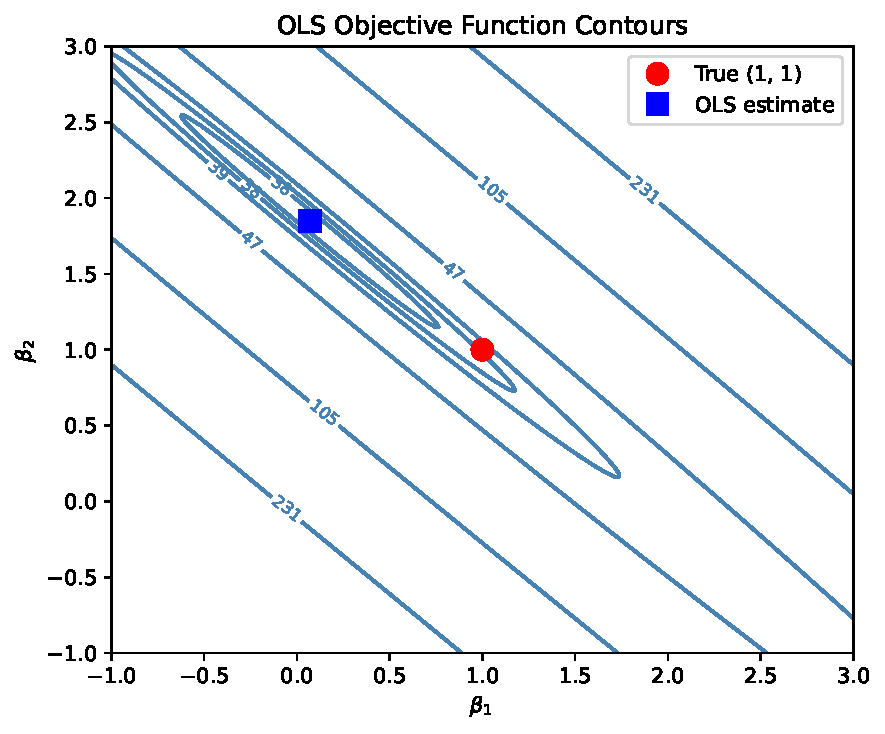
\includegraphics[keepaspectratio]{contents/1/shrinkage_files/figure-pdf/cell-9-output-1.pdf}}

The contour map reveals a narrow, elongated valley in the \(\rss\)
objective function. While the surface is highly sensitive to movement
perpendicular to the valley, it remains relatively flat along the valley
floor. Because the surface is particularly flat in this longitudinal
direction, numerous parameter combinations yield nearly identical
\(\rss\) values. Consequently, the data provides insufficient
information to distinguish between points along this axis, making the
\(\rss\) minimum highly unstable. This lack of identifiability is the
fundamental cause of high variance in the estimated coefficients.

When ridge regression is applied, the \(\rss\) objective function is
modified by adding a penalty term. As a result, the objective surface no
longer exhibits a long, flat valley floor. Instead, the minimum becomes
more well-defined, and the estimate is pulled toward the origin.
Although the true parameter may no longer lie at the bottom of this
modified valley, the ridge estimate has substantially lower variance. In
this way, ridge regression stabilizes the estimation by controlling the
region along the valley floor where the OLS solution would otherwise
vary widely.

Here we show the \(\rss\) objective function contours for
\(\lambda=0.1\), \(1\), \(10\) and \(100\).

\begin{Shaded}
\begin{Highlighting}[]
\ImportTok{from}\NormalTok{ sklearn.linear\_model }\ImportTok{import}\NormalTok{ Ridge}

\NormalTok{beta1\_vals }\OperatorTok{=}\NormalTok{ np.linspace(}\OperatorTok{{-}}\DecValTok{1}\NormalTok{, }\DecValTok{3}\NormalTok{, }\DecValTok{200}\NormalTok{)}
\NormalTok{beta2\_vals }\OperatorTok{=}\NormalTok{ np.linspace(}\OperatorTok{{-}}\DecValTok{1}\NormalTok{, }\DecValTok{3}\NormalTok{, }\DecValTok{200}\NormalTok{)}
\NormalTok{B1, B2 }\OperatorTok{=}\NormalTok{ np.meshgrid(beta1\_vals, beta2\_vals)}

\NormalTok{lambda\_vals }\OperatorTok{=}\NormalTok{ [}\FloatTok{0.1}\NormalTok{, }\DecValTok{1}\NormalTok{, }\DecValTok{10}\NormalTok{, }\DecValTok{100}\NormalTok{]}


\NormalTok{fig, axes }\OperatorTok{=}\NormalTok{ plt.subplots(}\DecValTok{2}\NormalTok{, }\DecValTok{2}\NormalTok{, figsize}\OperatorTok{=}\NormalTok{(}\DecValTok{10}\NormalTok{, }\DecValTok{8}\NormalTok{))}

\ControlFlowTok{for}\NormalTok{ ax, reg\_lambda }\KeywordTok{in} \BuiltInTok{zip}\NormalTok{(axes.ravel(), lambda\_vals):}
\NormalTok{    betas }\OperatorTok{=}\NormalTok{ np.column\_stack([B1.ravel(), B2.ravel()])}
\NormalTok{    preds }\OperatorTok{=}\NormalTok{ X }\OperatorTok{@}\NormalTok{ betas.T}
\NormalTok{    rss\_term }\OperatorTok{=}\NormalTok{ np.}\BuiltInTok{sum}\NormalTok{((y.reshape(}\OperatorTok{{-}}\DecValTok{1}\NormalTok{, }\DecValTok{1}\NormalTok{) }\OperatorTok{{-}}\NormalTok{ preds) }\OperatorTok{**} \DecValTok{2}\NormalTok{, axis}\OperatorTok{=}\DecValTok{0}\NormalTok{)}
\NormalTok{    penalty\_term }\OperatorTok{=}\NormalTok{ reg\_lambda }\OperatorTok{*}\NormalTok{ np.}\BuiltInTok{sum}\NormalTok{(betas}\OperatorTok{**}\DecValTok{2}\NormalTok{, axis}\OperatorTok{=}\DecValTok{1}\NormalTok{)}
\NormalTok{    rss\_value }\OperatorTok{=}\NormalTok{ (rss\_term }\OperatorTok{+}\NormalTok{ penalty\_term).reshape(B1.shape)}

\NormalTok{    quant\_levels }\OperatorTok{=}\NormalTok{ np.quantile(rss\_value, [}\FloatTok{0.01}\NormalTok{, }\FloatTok{0.025}\NormalTok{, }\FloatTok{0.05}\NormalTok{, }\FloatTok{0.2}\NormalTok{, }\FloatTok{0.5}\NormalTok{, }\FloatTok{0.75}\NormalTok{])}

\NormalTok{    cs }\OperatorTok{=}\NormalTok{ ax.contour(B1, B2, rss\_value, levels}\OperatorTok{=}\NormalTok{quant\_levels, colors}\OperatorTok{=}\StringTok{"steelblue"}\NormalTok{)}
\NormalTok{    ax.clabel(cs, inline}\OperatorTok{=}\VariableTok{True}\NormalTok{, fontsize}\OperatorTok{=}\DecValTok{7}\NormalTok{, fmt}\OperatorTok{=}\StringTok{"\%.0f"}\NormalTok{)}

\NormalTok{    ridge }\OperatorTok{=}\NormalTok{ Ridge(alpha}\OperatorTok{=}\NormalTok{reg\_lambda, fit\_intercept}\OperatorTok{=}\VariableTok{False}\NormalTok{).fit(X, y)}

\NormalTok{    ax.plot(}\DecValTok{1}\NormalTok{, }\DecValTok{1}\NormalTok{, }\StringTok{"ro"}\NormalTok{, markersize}\OperatorTok{=}\DecValTok{8}\NormalTok{, label}\OperatorTok{=}\StringTok{"True (1,1)"}\NormalTok{)}
\NormalTok{    ax.plot(ridge.coef\_[}\DecValTok{0}\NormalTok{], ridge.coef\_[}\DecValTok{1}\NormalTok{], }\StringTok{"bs"}\NormalTok{, markersize}\OperatorTok{=}\DecValTok{8}\NormalTok{, label}\OperatorTok{=}\StringTok{"Ridge"}\NormalTok{)}

\NormalTok{    ax.set\_title(}\VerbatimStringTok{r"}\DecValTok{$}\ErrorTok{\textbackslash{}}\VerbatimStringTok{lambda}\DecValTok{$}\VerbatimStringTok{ = \{\}"}\NormalTok{.}\BuiltInTok{format}\NormalTok{(reg\_lambda))}
\NormalTok{    ax.set\_xlabel(}\VerbatimStringTok{r"}\DecValTok{$\textbackslash{}b}\VerbatimStringTok{eta\_1}\DecValTok{$}\VerbatimStringTok{"}\NormalTok{)}
\NormalTok{    ax.set\_ylabel(}\VerbatimStringTok{r"}\DecValTok{$\textbackslash{}b}\VerbatimStringTok{eta\_2}\DecValTok{$}\VerbatimStringTok{"}\NormalTok{)}

\NormalTok{handles, labels }\OperatorTok{=}\NormalTok{ axes[}\DecValTok{0}\NormalTok{, }\DecValTok{0}\NormalTok{].get\_legend\_handles\_labels()}
\NormalTok{fig.suptitle(}\StringTok{"Ridge Objective Function Contours for Different lambda Values"}\NormalTok{)}
\NormalTok{fig.legend(handles, labels, loc}\OperatorTok{=}\StringTok{"right"}\NormalTok{)}
\NormalTok{plt.tight\_layout()}
\end{Highlighting}
\end{Shaded}

\pandocbounded{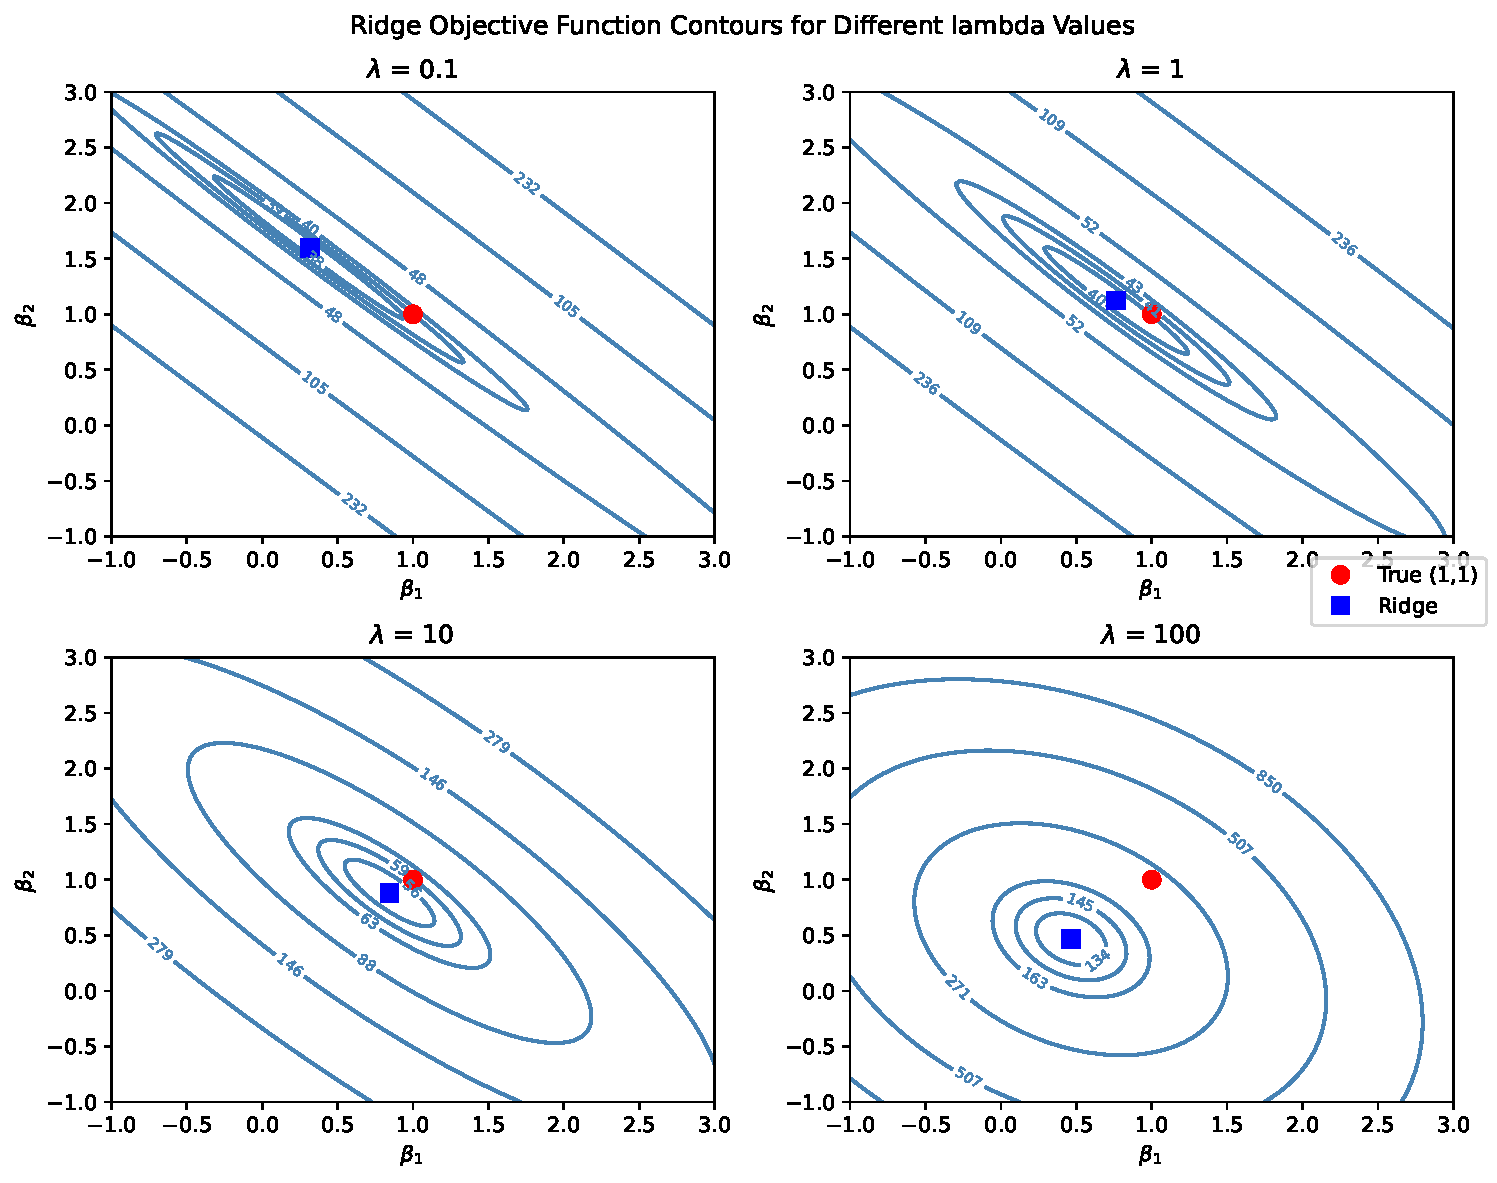
\includegraphics[keepaspectratio]{contents/1/shrinkage_files/figure-pdf/cell-10-output-1.pdf}}

As \(\lambda\) increases, the bottom of the valley gradually becomes
more rounded, and the objective surface rises more steeply as the
coefficients move away from the origin. This additional curvature
removes the long flat valley floor and makes the minimum more clearly
defined. At the same time, the penalty pulls the estimated coefficients
toward the origin, so the ridge estimate is effectively dragged toward
zero.

Geometrically, this shrinkage prevents the estimator from drifting
freely along the nearly flat valley direction that appears in the OLS
objective. As a result, the ridge estimator is much more stable and
typically has substantially lower variance than the OLS estimator,
although this improvement comes at the cost of introducing some bias.

\begin{tcolorbox}[enhanced jigsaw, arc=.35mm, bottomrule=.15mm, bottomtitle=1mm, breakable, colback=white, colbacktitle=quarto-callout-note-color!10!white, colframe=quarto-callout-note-color-frame, coltitle=black, left=2mm, leftrule=.75mm, opacityback=0, opacitybacktitle=0.6, rightrule=.15mm, title=\textcolor{quarto-callout-note-color}{\faInfo}\hspace{0.5em}{Gram matrix and Covariance matrix}, titlerule=0mm, toprule=.15mm, toptitle=1mm]

The Gram matrix \(X^\top X\) represents the raw inner products of
predictors. In the context of \(\rss\) map, it is the direct source of
the surface geometry.

The Covariance matrix is essentially the Gram matrix of the centered
data, usually scaled by \(n-1\). \[
\mathbf{S} = \frac{1}{n-1} \sum (x_i - \bar{x})(x_i - \bar{x})^top.
\]

Therefore if the data is already centered, the Gram matrix and the
covariance matrix are directly related: \(X^\top X=(n-1)\Cov\).

Mathematically, these two directions (the longitudinal axis and the
perpendicular axis) correspond to the eigenvectors of the
\(\mathbf{X}^T\mathbf{X}\) matrix (or, equivalently, the principal
components of the predictor space). The flatness or steepness in those
directions is governed by their corresponding eigenvalues.

\begin{Shaded}
\begin{Highlighting}[]
\NormalTok{XTX }\OperatorTok{=}\NormalTok{ X.T }\OperatorTok{@}\NormalTok{ X}
\NormalTok{eigenvalues, eigenvectors }\OperatorTok{=}\NormalTok{ np.linalg.eigh(XTX)}
\ControlFlowTok{for}\NormalTok{ i }\KeywordTok{in} \BuiltInTok{range}\NormalTok{(}\BuiltInTok{len}\NormalTok{(eigenvalues)):}
    \BuiltInTok{print}\NormalTok{(}\SpecialStringTok{f\textquotesingle{}eigenvalue: }\SpecialCharTok{\{}\NormalTok{eigenvalues[i]}\SpecialCharTok{: .2f\}}\SpecialStringTok{, eigenbasis: }\SpecialCharTok{\{}\NormalTok{eigenvectors[i]}\SpecialCharTok{\}}\SpecialStringTok{\textquotesingle{}}\NormalTok{)}
\end{Highlighting}
\end{Shaded}

\begin{verbatim}
eigenvalue:  0.26, eigenbasis: [ 0.70320986 -0.71098234]
eigenvalue:  95.19, eigenbasis: [-0.71098234 -0.70320986]
\end{verbatim}

Then mark the eigenvectors in the contour map.

\begin{Shaded}
\begin{Highlighting}[]
\NormalTok{fig, ax }\OperatorTok{=}\NormalTok{ plt.subplots(figsize}\OperatorTok{=}\NormalTok{(}\DecValTok{6}\NormalTok{, }\DecValTok{5}\NormalTok{))}

\NormalTok{quant\_levels }\OperatorTok{=}\NormalTok{ np.quantile(rss\_value0, [}\FloatTok{0.01}\NormalTok{, }\FloatTok{0.025}\NormalTok{, }\FloatTok{0.05}\NormalTok{, }\FloatTok{0.2}\NormalTok{, }\FloatTok{0.5}\NormalTok{, }\FloatTok{0.75}\NormalTok{])}
\NormalTok{cs }\OperatorTok{=}\NormalTok{ ax.contour(B1, B2, rss\_value0, levels}\OperatorTok{=}\NormalTok{quant\_levels, colors}\OperatorTok{=}\StringTok{"lightblue"}\NormalTok{)}
\NormalTok{ax.clabel(cs, inline}\OperatorTok{=}\VariableTok{True}\NormalTok{, fontsize}\OperatorTok{=}\DecValTok{8}\NormalTok{, fmt}\OperatorTok{=}\StringTok{"\%.0f"}\NormalTok{)}

\NormalTok{ax.plot(}\DecValTok{1}\NormalTok{, }\DecValTok{1}\NormalTok{, }\StringTok{"ro"}\NormalTok{, markersize}\OperatorTok{=}\DecValTok{10}\NormalTok{, label}\OperatorTok{=}\StringTok{"True (1, 1)"}\NormalTok{)}
\NormalTok{ax.plot(ols.coef\_[}\DecValTok{0}\NormalTok{], ols.coef\_[}\DecValTok{1}\NormalTok{], }\StringTok{"bs"}\NormalTok{, markersize}\OperatorTok{=}\DecValTok{10}\NormalTok{, label}\OperatorTok{=}\StringTok{"OLS estimate"}\NormalTok{)}

\NormalTok{scale }\OperatorTok{=} \FloatTok{0.6}
\ControlFlowTok{for}\NormalTok{ i }\KeywordTok{in} \BuiltInTok{range}\NormalTok{(}\BuiltInTok{len}\NormalTok{(eigenvalues)):}
\NormalTok{    v }\OperatorTok{=}\NormalTok{ eigenvectors[:, i]}
\NormalTok{    ax.arrow(}
\NormalTok{        ols.coef\_[}\DecValTok{0}\NormalTok{],}
\NormalTok{        ols.coef\_[}\DecValTok{1}\NormalTok{],}
\NormalTok{        v[}\DecValTok{0}\NormalTok{] }\OperatorTok{*}\NormalTok{ scale,}
\NormalTok{        v[}\DecValTok{1}\NormalTok{] }\OperatorTok{*}\NormalTok{ scale,}
\NormalTok{        head\_width}\OperatorTok{=}\FloatTok{0.05}\NormalTok{,}
\NormalTok{        head\_length}\OperatorTok{=}\FloatTok{0.1}\NormalTok{,}
\NormalTok{        fc}\OperatorTok{=}\StringTok{"orange"}\NormalTok{,}
\NormalTok{        ec}\OperatorTok{=}\StringTok{"orange"}\NormalTok{,}
\NormalTok{        label}\OperatorTok{=}\StringTok{"Eigenvectors"} \ControlFlowTok{if}\NormalTok{ i }\OperatorTok{==} \DecValTok{0} \ControlFlowTok{else} \StringTok{""}\NormalTok{,}
\NormalTok{    )}

\NormalTok{    ax.text(}
\NormalTok{        ols.coef\_[}\DecValTok{0}\NormalTok{] }\OperatorTok{+}\NormalTok{ v[}\DecValTok{0}\NormalTok{] }\OperatorTok{*}\NormalTok{ scale }\OperatorTok{*} \FloatTok{1.5}\NormalTok{,}
\NormalTok{        ols.coef\_[}\DecValTok{1}\NormalTok{] }\OperatorTok{+}\NormalTok{ v[}\DecValTok{1}\NormalTok{] }\OperatorTok{*}\NormalTok{ scale }\OperatorTok{*} \FloatTok{1.5}\NormalTok{,}
        \VerbatimStringTok{r"}\DecValTok{$}\VerbatimStringTok{v\_\{\}}\DecValTok{$}\VerbatimStringTok{ }\KeywordTok{(}\DecValTok{$}\ErrorTok{\textbackslash{}}\VerbatimStringTok{lambda=\{:}\DecValTok{.}\VerbatimStringTok{2f\}}\DecValTok{$}\KeywordTok{)}\VerbatimStringTok{"}\NormalTok{.}\BuiltInTok{format}\NormalTok{(i }\OperatorTok{+} \DecValTok{1}\NormalTok{, eigenvalues[i]),}
\NormalTok{        color}\OperatorTok{=}\StringTok{"darkorange"}\NormalTok{,}
\NormalTok{        fontweight}\OperatorTok{=}\StringTok{"bold"}\NormalTok{,}
\NormalTok{        ha}\OperatorTok{=}\StringTok{"center"}\NormalTok{,}
\NormalTok{    )}
\NormalTok{ax.legend()}
\NormalTok{plt.tight\_layout()}
\end{Highlighting}
\end{Shaded}

\pandocbounded{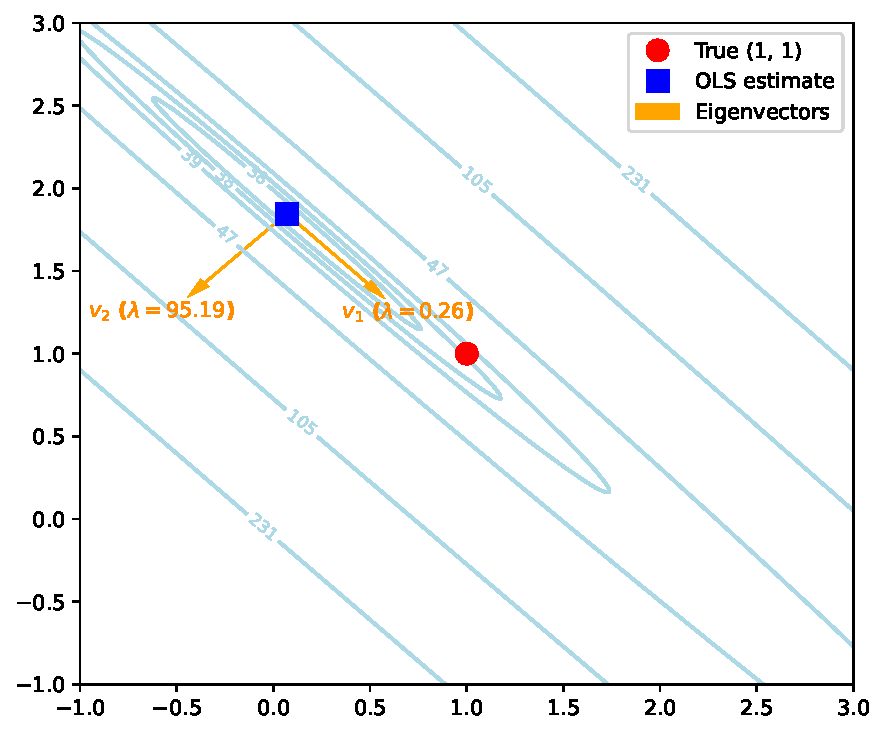
\includegraphics[keepaspectratio]{contents/1/shrinkage_files/figure-pdf/cell-12-output-1.pdf}}

\end{tcolorbox}

\subsection{\texorpdfstring{Choosing
\(\lambda\)}{Choosing \textbackslash lambda}}\label{choosing-lambda}

The regularization parameter \(\lambda\) determines how much shrinkage
is applied.

In practice, the modern standard is to choose \(\lambda\) by
cross-validation. Similar to the model selection procedure discussed in
the linear regression case, the process works as follows:

\begin{enumerate}
\def\labelenumi{\arabic{enumi}.}
\tightlist
\item
  Fix a value of \(\lambda\). Split the dataset into \(k\) folds. Each
  time, choose one fold as the validation set and use the remaining
  folds as the training set to fit the model and compute the validation
  score.
\item
  Repeat this process so that each fold serves once as the validation
  set. The average validation score is the cross-validation score for
  this \(\lambda\).
\item
  Repeat the above steps for each candidate value of \(\lambda\), and
  select the \(\lambda\) with the best cross-validation score.
\item
  Finally, refit the model on the entire training set using the selected
  \(\lambda\).
\end{enumerate}

Since this procedure is very common in ridge regression, sklearn
provides \texttt{RidgeCV}, which has built-in cross-validation.
Alternatively, the same task can be performed using
\texttt{GridSearchCV}.

\begin{tcolorbox}[enhanced jigsaw, arc=.35mm, bottomrule=.15mm, bottomtitle=1mm, breakable, colback=white, colbacktitle=quarto-callout-note-color!10!white, colframe=quarto-callout-note-color-frame, coltitle=black, left=2mm, leftrule=.75mm, opacityback=0, opacitybacktitle=0.6, rightrule=.15mm, title=\textcolor{quarto-callout-note-color}{\faInfo}\hspace{0.5em}{Leave-one-out cross-validation}, titlerule=0mm, toprule=.15mm, toptitle=1mm]

\texttt{GridSearchCV} typically uses \(k\)-fold cross-validation, where
the training set is split into \(k\) folds and each fold is used once as
the validation set.

If each observation is treated as its own fold (that is, the validation
set contains exactly one observation), the procedure is called
leave-one-out cross-validation (LOOCV). In other words, LOOCV is
equivalent to \(N\)-fold cross-validation, where \(N\) is the number of
observations.

\texttt{RidgeCV} uses leave-one-out cross-validation by default.

\end{tcolorbox}

The arguments of \texttt{RidgeCV} are similar to those of
\texttt{Ridge}. The main differences are:

\begin{itemize}
\tightlist
\item
  \texttt{alphas} should be a list of candidate values for \(\alpha\).
  In the example below, \(\alpha\) is selected from values ranging from
  \texttt{1e-4} to \texttt{1e4}.
\item
  \texttt{cv} works in the same way as in ordinary cross-validation and
  specifies the number of folds used in the cross-validation procedure.
  If it is not set, LOOCV will be used.
\end{itemize}

\begin{Shaded}
\begin{Highlighting}[]
\ImportTok{from}\NormalTok{ sklearn.linear\_model }\ImportTok{import}\NormalTok{ RidgeCV}
\ImportTok{from}\NormalTok{ sklearn.pipeline }\ImportTok{import}\NormalTok{ Pipeline}
\ImportTok{from}\NormalTok{ sklearn.preprocessing }\ImportTok{import}\NormalTok{ StandardScaler}

\NormalTok{alphas }\OperatorTok{=}\NormalTok{ np.logspace(}\OperatorTok{{-}}\DecValTok{4}\NormalTok{, }\DecValTok{4}\NormalTok{, }\DecValTok{100}\NormalTok{)}

\NormalTok{ridge\_cv\_pipe }\OperatorTok{=}\NormalTok{ Pipeline(}
\NormalTok{    [}
\NormalTok{        (}\StringTok{"scaler"}\NormalTok{, StandardScaler()),}
\NormalTok{        (}\StringTok{"model"}\NormalTok{, RidgeCV(alphas}\OperatorTok{=}\NormalTok{alphas)),}
\NormalTok{    ]}
\NormalTok{)}

\NormalTok{ridge\_cv\_pipe.fit(X, y)}

\NormalTok{best\_alpha\_ridge }\OperatorTok{=}\NormalTok{ ridge\_cv\_pipe.named\_steps[}\StringTok{"model"}\NormalTok{].alpha\_}
\NormalTok{best\_alpha\_ridge}
\end{Highlighting}
\end{Shaded}

\begin{verbatim}
1.3219411484660315
\end{verbatim}

\subsection{Validation curve and Coefficient
paths}\label{validation-curve-and-coefficient-paths}

\texttt{RidgeCV} returns only the final fitted model at the selected
value of \texttt{alpha}, rather than the entire validation curve or
coefficient path. If we want to examine how the validation score changes
with \texttt{alpha}, we may fit ordinary Ridge models over a grid of
\texttt{alpha} values and then add a vertical line at the value selected
by \texttt{RidgeCV}.

\texttt{sklearn} provides \texttt{validation\_curve()} to streamline the
process.

\protect\phantomsection\label{annotated-cell-75}%
\begin{Shaded}
\begin{Highlighting}[]
\ImportTok{from}\NormalTok{ sklearn.model\_selection }\ImportTok{import}\NormalTok{ validation\_curve}

\NormalTok{alphas }\OperatorTok{=}\NormalTok{ np.logspace(}\OperatorTok{{-}}\DecValTok{4}\NormalTok{, }\DecValTok{4}\NormalTok{, }\DecValTok{100}\NormalTok{)}

\NormalTok{ridge\_pipe }\OperatorTok{=}\NormalTok{ Pipeline(}
\NormalTok{    [}
\NormalTok{        (}\StringTok{"scaler"}\NormalTok{, StandardScaler()),}
\NormalTok{        (}\StringTok{"model"}\NormalTok{, Ridge()),}
\NormalTok{    ]}
\NormalTok{)}
\NormalTok{train\_scores, test\_scores }\OperatorTok{=}\NormalTok{ validation\_curve(}
\NormalTok{    ridge\_pipe, X, y, param\_name}\OperatorTok{=}\StringTok{"model\_\_alpha"}\NormalTok{, param\_range}\OperatorTok{=}\NormalTok{alphas}
\NormalTok{) }\CommentTok{\# \textless{}1\textgreater{}}

\NormalTok{plt.plot(alphas, train\_scores.mean(axis}\OperatorTok{=}\DecValTok{1}\NormalTok{), label}\OperatorTok{=}\StringTok{"train"}\NormalTok{)}
\NormalTok{plt.plot(alphas, test\_scores.mean(axis}\OperatorTok{=}\DecValTok{1}\NormalTok{), label}\OperatorTok{=}\StringTok{"test"}\NormalTok{)}
\NormalTok{plt.axvline(best\_alpha\_ridge, color}\OperatorTok{=}\StringTok{"black"}\NormalTok{, linestyle}\OperatorTok{=}\StringTok{"{-}{-}"}\NormalTok{, label}\OperatorTok{=}\StringTok{"LOOCV alpha"}\NormalTok{) }\CommentTok{\# \textless{}2\textgreater{}}
\NormalTok{plt.xscale(}\StringTok{"log"}\NormalTok{)}
\NormalTok{plt.xlabel(}\StringTok{"alpha"}\NormalTok{)}
\NormalTok{plt.ylabel(}\StringTok{"score"}\NormalTok{)}
\NormalTok{plt.title(}\StringTok{"Validation curve for ridge regression"}\NormalTok{)}
\NormalTok{plt.legend()}
\end{Highlighting}
\end{Shaded}

\begin{description}
\tightlist
\item[5CB6E08D-list-annote-1]
The validation curve can also be drawn using
\texttt{GridSearchCV.cv\_results\_}. There is no major difference
between the two methods.
\item[5CB6E08D-list-annote-2]
This best \texttt{alpha} here is based on the LOOCV formula. So it is
slightly different from the best \texttt{alpha} under 5-fold
cross-validation.
\end{description}

\pandocbounded{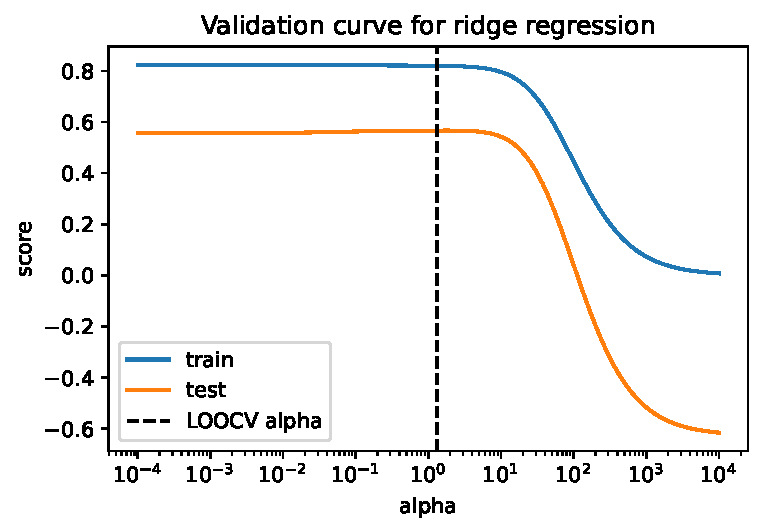
\includegraphics[keepaspectratio]{contents/1/shrinkage_files/figure-pdf/cell-14-output-1.pdf}}

Similarly, if we want to examine how the coefficients change with
\texttt{alpha}, we fit ordinary \texttt{Ridge} repeatedly over a grid of
\texttt{alpha} values and record the fitted coefficients. In this case,
cross-validation is not needed, since the goal is only to visualize the
coefficient path rather than to compare models.

\protect\phantomsection\label{annotated-cell-76}%
\begin{Shaded}
\begin{Highlighting}[]
\ImportTok{from}\NormalTok{ sklearn.linear\_model }\ImportTok{import}\NormalTok{ Ridge}
\ImportTok{import}\NormalTok{ matplotlib.pyplot }\ImportTok{as}\NormalTok{ plt}

\NormalTok{alphas }\OperatorTok{=}\NormalTok{ np.logspace(}\OperatorTok{{-}}\DecValTok{4}\NormalTok{, }\DecValTok{4}\NormalTok{, }\DecValTok{100}\NormalTok{)}
\NormalTok{coefs }\OperatorTok{=}\NormalTok{ []}
\ControlFlowTok{for}\NormalTok{ a }\KeywordTok{in}\NormalTok{ alphas:}
\NormalTok{    pipe }\OperatorTok{=}\NormalTok{ Pipeline(}
\NormalTok{        [}
\NormalTok{            (}\StringTok{"scaler"}\NormalTok{, StandardScaler()),}
\NormalTok{            (}\StringTok{"model"}\NormalTok{, Ridge(alpha}\OperatorTok{=}\NormalTok{a)),}
\NormalTok{        ]}
\NormalTok{    )}
\NormalTok{    pipe.fit(X, y)}
\NormalTok{    coefs.append(pipe.named\_steps[}\StringTok{"model"}\NormalTok{].coef\_)}
\NormalTok{coefs }\OperatorTok{=}\NormalTok{ np.array(coefs)}
\ControlFlowTok{for}\NormalTok{ j }\KeywordTok{in} \BuiltInTok{range}\NormalTok{(coefs.shape[}\DecValTok{1}\NormalTok{]):}
\NormalTok{    plt.plot(alphas, coefs[:, j], label}\OperatorTok{=}\SpecialStringTok{f"x}\SpecialCharTok{\{}\NormalTok{j }\OperatorTok{+} \DecValTok{1}\SpecialCharTok{\}}\SpecialStringTok{"}\NormalTok{)}
\NormalTok{plt.axvline(best\_alpha\_ridge, linestyle}\OperatorTok{=}\StringTok{"{-}{-}"}\NormalTok{, color}\OperatorTok{=}\StringTok{"black"}\NormalTok{, label}\OperatorTok{=}\StringTok{"RidgeCV alpha"}\NormalTok{)}

\NormalTok{ax }\OperatorTok{=}\NormalTok{ plt.gca()}
\NormalTok{ax.set\_xlim(ax.get\_xlim()[::}\OperatorTok{{-}}\DecValTok{1}\NormalTok{]) }\CommentTok{\# \textless{}1\textgreater{}}
\NormalTok{plt.xscale(}\StringTok{"log"}\NormalTok{)}
\NormalTok{plt.xlabel(}\StringTok{"alpha"}\NormalTok{)}
\NormalTok{plt.ylabel(}\StringTok{"weights"}\NormalTok{)}
\NormalTok{plt.title(}\StringTok{"Ridge Coefficients vs Regularization Strength (alpha)"}\NormalTok{)}
\NormalTok{plt.axis(}\StringTok{"tight"}\NormalTok{)}
\NormalTok{plt.legend()}
\end{Highlighting}
\end{Shaded}

\begin{description}
\tightlist
\item[5CB6E08D-list-annote-1]
In the coefficient path plot, the horizontal axis is shown in reverse
order so that the coefficients move from heavily regularized models on
the left to weakly regularized models on the right.
\end{description}

\pandocbounded{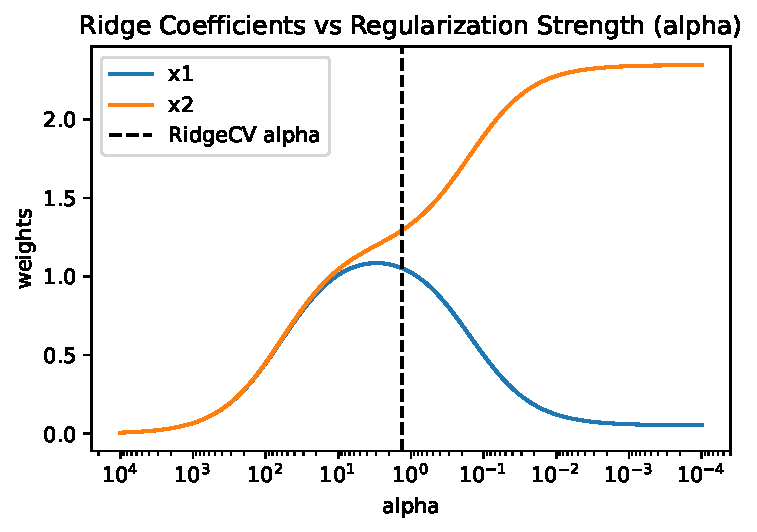
\includegraphics[keepaspectratio]{contents/1/shrinkage_files/figure-pdf/cell-15-output-1.pdf}}

\subsection{LOOCV}\label{loocv}

Naively, LOOCV would require fitting the model \(N\) times. Each time
one observation is removed and the model is refit. However, ridge
regression admits an analytic formula that allows the LOOCV error to be
computed without refitting the model repeatedly. This is one reason
ridge regression works very well with LOOCV. \texttt{RidgeCV} from
\texttt{sklearn} is also implemented using LOOCV formula instead of
refitting the model multiple times.

\begin{theorem}[LOOCV]\protect\hypertarget{thm-}{}\label{thm-}

The LOOCV error is \[
\text{CV}(\lambda)
=
\frac{1}{N}
\sum_{i=1}^{N}
\qty(
\frac{y_i - \hat{y}_i}{1 - H_{\lambda,ii}}
)^2.
\]

Click for proof.

Recall that the ridge estimator is \[
\hat{\beta}_\lambda = (X^\top X + \lambda I)^{-1} X^\top y.
\]

The fitted values can be written as \[
\hat{y} = X\hat{\beta}_\lambda = H_\lambda y,
\] where \[
H_\lambda = X (X^\top X + \lambda I)^{-1} X^\top
\] is the ridge hat matrix.

Let

\[
r_i = y_i - \hat{y}_i
\]

be the ordinary residual from the ridge regression fitted using the
entire dataset.

Suppose we remove observation \(i\) and refit the ridge regression
model. Let \(\hat{y}_{(i)}\) denote the predicted value for \(y_i\) from
this leave-one-out model. The corresponding leave-one-out residual is

\[
r_{(i)} = y_i - \hat{y}_{(i)} .
\]

By the PRESS residual formula {[}4{]}, this residual can be computed
directly from the full-data fit: \[
r_{(i)} = \frac{r_i}{1 - H_{\lambda,ii}} ,
\]

where \(H_{\lambda,ii}\) is the \(i\)-th diagonal element of the ridge
hat matrix.

Therefore the LOOCV error is \[
\text{CV}(\lambda)
=
\frac{1}{N}
\sum_{i=1}^{N}
\qty(
\frac{y_i - \hat{y}_i}{1 - H_{\lambda,ii}}
)^2.
\]

\end{theorem}

\begin{tcolorbox}[enhanced jigsaw, arc=.35mm, bottomrule=.15mm, bottomtitle=1mm, breakable, colback=white, colbacktitle=quarto-callout-note-color!10!white, colframe=quarto-callout-note-color-frame, coltitle=black, left=2mm, leftrule=.75mm, opacityback=0, opacitybacktitle=0.6, rightrule=.15mm, title=\textcolor{quarto-callout-note-color}{\faInfo}\hspace{0.5em}{Note}, titlerule=0mm, toprule=.15mm, toptitle=1mm]

This formula means that the leave-one-out residuals can be obtained by
simply adjusting the ordinary residuals using the leverage term
\(H_{\lambda,ii}\). Consequently, the LOOCV error can be computed
without refitting the model \(N\) times.

\end{tcolorbox}

\section{Lasso Regression}\label{lasso-regression}

\subsection{Definition}\label{definition}

Lasso regression (short for least absolute shrinkage and selection
operator) modifies the OLS objective by adding an \(L_1\) penalty.

\begin{definition}[Lasso
Regression]\protect\hypertarget{def-lasso}{}\label{def-lasso}

For a response vector \(y \in \mathbb{R}^n\) and a design matrix
\(X \in \mathbb{R}^{n \times p}\), the lasso estimator
\(\hat{\beta}_{\lasso}\) is defined by

\[
\hat{\beta}_{\lasso}
=
\arg\min_{\beta}
\qty{
\norm{y-X\beta}_2^2 + \lambda \norm{\beta}_1
}
\]

where

\begin{itemize}
\tightlist
\item
  \(\lambda \ge 0\) is the regularization parameter,
\item
  \(\norm{\beta}_1 = \sum_{j=1}^p |\beta_j|\) is the \(L_1\) norm of the
  coefficient vector.
\end{itemize}

\end{definition}

\begin{tcolorbox}[enhanced jigsaw, arc=.35mm, bottomrule=.15mm, bottomtitle=1mm, breakable, colback=white, colbacktitle=quarto-callout-note-color!10!white, colframe=quarto-callout-note-color-frame, coltitle=black, left=2mm, leftrule=.75mm, opacityback=0, opacitybacktitle=0.6, rightrule=.15mm, title=\textcolor{quarto-callout-note-color}{\faInfo}\hspace{0.5em}{Solving lasso}, titlerule=0mm, toprule=.15mm, toptitle=1mm]

Lasso is solved using numerical optimization algorithms. The most widely
used methods include

\begin{itemize}
\tightlist
\item
  coordinate descent
\item
  LARS (Least Angle Regression)
\item
  proximal gradient methods
\end{itemize}

These algorithms iteratively update the coefficients until convergence.

Unlike OLS or ridge regression, the lasso estimator does not admit a
closed-form solution because the \(L_1\) penalty is not differentiable
at zero.

\end{tcolorbox}

The lasso penalty also shrinks the coefficients toward zero, and
therefore behaves similarly to ridge regression. In practice, the
penalty is typically applied only to the slope coefficients, so the
intercept is not penalized. For this reason, it is common to standardize
the predictors and center the response variable before fitting the
model.

However, lasso has an important difference from ridge regression, which
we discuss in the next section.

\subsection{Geometry and sparsity}\label{geometry-and-sparsity}

Similar to ridge regression, by the theory of Lagrange multipliers,
lasso can also be written in constrained form:

\[
\hat{\beta}_{\lasso}
=
\arg\min_{\beta}
\norm{y-X\beta}_2^2
\quad
\text{subject to}
\quad
\norm{\beta}_1 \le s.
\]

Here \(s \ge 0\) controls the size of the coefficient vector. This
constrained formulation is useful because it makes the geometry of lasso
easier to visualize.

In \(\mathbb{R}^2\), the ridge constraint region is based on the \(L_2\)
norm and has a circular boundary, whereas the lasso constraint region is
based on the \(L_1\) norm and has a diamond-shaped boundary. The
solution is obtained where the smallest residual \(\rss\) contour first
touches the constraint region.

For ridge regression, the circular boundary is smooth, so the point of
tangency typically occurs away from the coordinate axes. As a result,
ridge usually shrinks coefficients continuously toward zero, but does
not make them exactly zero.

For lasso, the diamond-shaped boundary has sharp corners lying on the
coordinate axes. Because of these corners, the point of tangency is much
more likely to occur at a location where one coordinate is zero.
Consequently, lasso can produce solutions with some coefficients exactly
equal to zero.

Therefore, ridge is mainly a shrinkage method, whereas lasso is both a
shrinkage method and a variable-selection method.

\begin{Shaded}
\begin{Highlighting}[]
\ImportTok{import}\NormalTok{ numpy }\ImportTok{as}\NormalTok{ np}
\ImportTok{import}\NormalTok{ matplotlib.pyplot }\ImportTok{as}\NormalTok{ plt}

\NormalTok{mu }\OperatorTok{=}\NormalTok{ np.array([}\FloatTok{2.0}\NormalTok{, }\FloatTok{0.35}\NormalTok{])}

\NormalTok{theta }\OperatorTok{=}\NormalTok{ np.deg2rad(}\DecValTok{32}\NormalTok{)}
\NormalTok{R }\OperatorTok{=}\NormalTok{ np.array([[np.cos(theta), }\OperatorTok{{-}}\NormalTok{np.sin(theta)], [np.sin(theta), np.cos(theta)]])}

\NormalTok{D }\OperatorTok{=}\NormalTok{ np.diag([}\FloatTok{7.0}\NormalTok{, }\FloatTok{0.45}\NormalTok{])}
\NormalTok{A }\OperatorTok{=}\NormalTok{ R }\OperatorTok{@}\NormalTok{ D }\OperatorTok{@}\NormalTok{ R.T}


\KeywordTok{def}\NormalTok{ rss(beta1, beta2):}
\NormalTok{    B }\OperatorTok{=}\NormalTok{ np.stack([beta1 }\OperatorTok{{-}}\NormalTok{ mu[}\DecValTok{0}\NormalTok{], beta2 }\OperatorTok{{-}}\NormalTok{ mu[}\DecValTok{1}\NormalTok{]], axis}\OperatorTok{={-}}\DecValTok{1}\NormalTok{)}
    \ControlFlowTok{return}\NormalTok{ np.einsum(}\StringTok{"...i,ij,...j{-}\textgreater{}..."}\NormalTok{, B, A, B)}


\NormalTok{x }\OperatorTok{=}\NormalTok{ np.linspace(}\OperatorTok{{-}}\FloatTok{0.5}\NormalTok{, }\FloatTok{3.2}\NormalTok{, }\DecValTok{600}\NormalTok{)}
\NormalTok{y }\OperatorTok{=}\NormalTok{ np.linspace(}\OperatorTok{{-}}\FloatTok{2.0}\NormalTok{, }\FloatTok{2.0}\NormalTok{, }\DecValTok{600}\NormalTok{)}
\NormalTok{X, Y }\OperatorTok{=}\NormalTok{ np.meshgrid(x, y)}
\NormalTok{Z }\OperatorTok{=}\NormalTok{ rss(X, Y)}

\NormalTok{levels }\OperatorTok{=}\NormalTok{ [}\FloatTok{0.15}\NormalTok{, }\FloatTok{0.4}\NormalTok{, }\FloatTok{0.8}\NormalTok{, }\FloatTok{1.4}\NormalTok{, }\FloatTok{2.4}\NormalTok{, }\FloatTok{3.8}\NormalTok{, }\FloatTok{5.8}\NormalTok{]}

\NormalTok{ridge\_r }\OperatorTok{=} \FloatTok{1.7}
\NormalTok{lasso\_t }\OperatorTok{=} \FloatTok{2.0}

\NormalTok{fig, axs }\OperatorTok{=}\NormalTok{ plt.subplots(}\DecValTok{1}\NormalTok{, }\DecValTok{2}\NormalTok{, figsize}\OperatorTok{=}\NormalTok{(}\DecValTok{10}\NormalTok{, }\DecValTok{5}\NormalTok{))}

\NormalTok{axs[}\DecValTok{0}\NormalTok{].contour(X, Y, Z, levels}\OperatorTok{=}\NormalTok{levels)}
\NormalTok{diamond }\OperatorTok{=}\NormalTok{ np.array(}
\NormalTok{    [[lasso\_t, }\DecValTok{0}\NormalTok{], [}\DecValTok{0}\NormalTok{, lasso\_t], [}\OperatorTok{{-}}\NormalTok{lasso\_t, }\DecValTok{0}\NormalTok{], [}\DecValTok{0}\NormalTok{, }\OperatorTok{{-}}\NormalTok{lasso\_t], [lasso\_t, }\DecValTok{0}\NormalTok{]]}
\NormalTok{)}
\NormalTok{axs[}\DecValTok{0}\NormalTok{].plot(diamond[:, }\DecValTok{0}\NormalTok{], diamond[:, }\DecValTok{1}\NormalTok{], linewidth}\OperatorTok{=}\DecValTok{3}\NormalTok{)}
\NormalTok{axs[}\DecValTok{0}\NormalTok{].scatter(}\OperatorTok{*}\NormalTok{mu)}
\NormalTok{axs[}\DecValTok{0}\NormalTok{].axhline(}\DecValTok{0}\NormalTok{)}
\NormalTok{axs[}\DecValTok{0}\NormalTok{].axvline(}\DecValTok{0}\NormalTok{)}
\NormalTok{axs[}\DecValTok{0}\NormalTok{].set\_title(}\StringTok{"Lasso Constraint"}\NormalTok{)}

\NormalTok{axs[}\DecValTok{1}\NormalTok{].contour(X, Y, Z, levels}\OperatorTok{=}\NormalTok{levels)}
\NormalTok{t }\OperatorTok{=}\NormalTok{ np.linspace(}\DecValTok{0}\NormalTok{, }\DecValTok{2} \OperatorTok{*}\NormalTok{ np.pi, }\DecValTok{400}\NormalTok{)}
\NormalTok{axs[}\DecValTok{1}\NormalTok{].plot(ridge\_r }\OperatorTok{*}\NormalTok{ np.cos(t), ridge\_r }\OperatorTok{*}\NormalTok{ np.sin(t), linewidth}\OperatorTok{=}\DecValTok{3}\NormalTok{)}
\NormalTok{axs[}\DecValTok{1}\NormalTok{].scatter(}\OperatorTok{*}\NormalTok{mu)}
\NormalTok{axs[}\DecValTok{1}\NormalTok{].axhline(}\DecValTok{0}\NormalTok{)}
\NormalTok{axs[}\DecValTok{1}\NormalTok{].axvline(}\DecValTok{0}\NormalTok{)}
\NormalTok{axs[}\DecValTok{1}\NormalTok{].set\_title(}\StringTok{"Ridge Constraint"}\NormalTok{)}

\ControlFlowTok{for}\NormalTok{ ax }\KeywordTok{in}\NormalTok{ axs:}
\NormalTok{    ax.set\_xlim(}\OperatorTok{{-}}\FloatTok{2.2}\NormalTok{, }\FloatTok{3.2}\NormalTok{)}
\NormalTok{    ax.set\_ylim(}\OperatorTok{{-}}\DecValTok{2}\NormalTok{, }\DecValTok{2}\NormalTok{)}
\NormalTok{    ax.set\_aspect(}\StringTok{"equal"}\NormalTok{)}
\NormalTok{    ax.set\_xlabel(}\VerbatimStringTok{r"}\DecValTok{$\textbackslash{}b}\VerbatimStringTok{eta\_1}\DecValTok{$}\VerbatimStringTok{"}\NormalTok{)}
\NormalTok{    ax.set\_ylabel(}\VerbatimStringTok{r"}\DecValTok{$\textbackslash{}b}\VerbatimStringTok{eta\_2}\DecValTok{$}\VerbatimStringTok{"}\NormalTok{)}

\NormalTok{plt.tight\_layout()}
\end{Highlighting}
\end{Shaded}

\pandocbounded{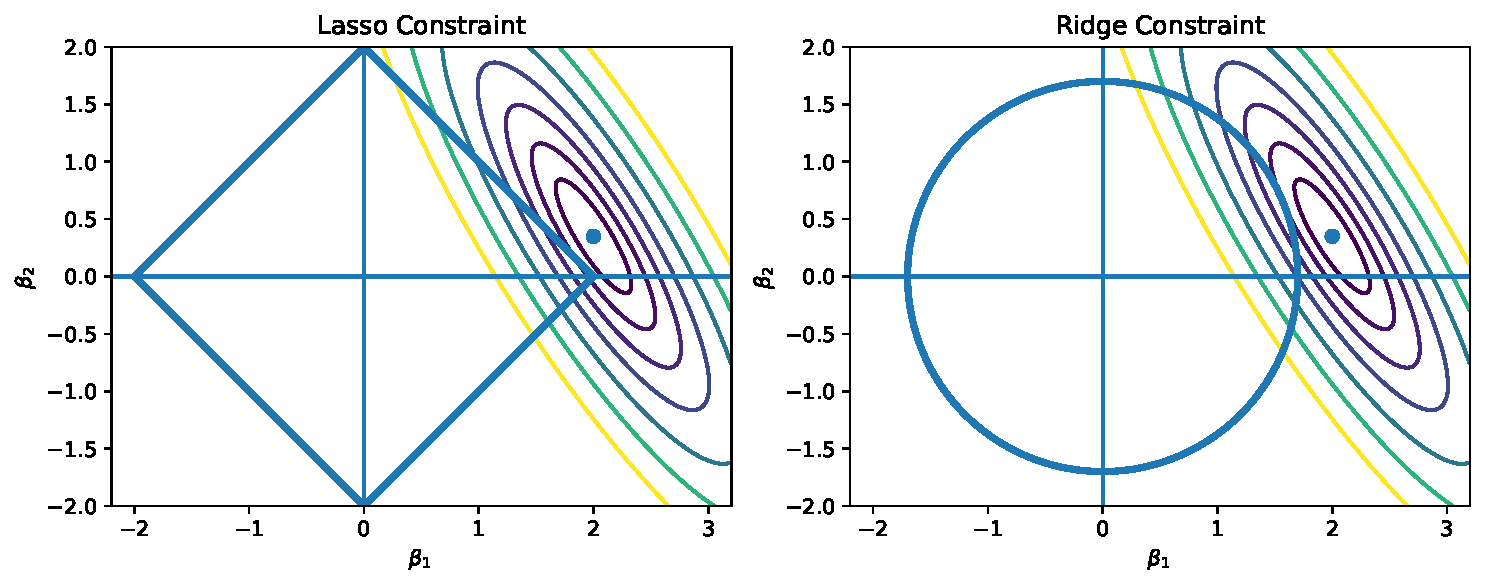
\includegraphics[keepaspectratio]{contents/1/shrinkage_files/figure-pdf/cell-16-output-1.pdf}}

\subsection{One-variable lasso and
soft-thresholding}\label{one-variable-lasso-and-soft-thresholding}

To understand how lasso sets coefficients to \(0\), it is useful to
first look at the one-variable case.

Suppose we want to solve \[
\min_{\beta}\qty{\norm{y-X\beta}_2^2 + \lambda \abs{\beta}}.
\]

Note that \[
\hat\beta_\ols=\arg\min_\beta\qty{\norm{y-X\beta}_2^2}
\] denotes the OLS solution for this one-variable problem.

\begin{theorem}[Soft-thresholding
Rule]\protect\hypertarget{thm-}{}\label{thm-}

\[
\hat\beta_\lasso=\begin{cases}
\hat\beta_\ols+\frac\lambda{2a}& \text{ if }\hat\beta_\ols<-\frac\lambda{2a},\\
0& \text{ if }\abs{\hat\beta_\ols}\leq\frac\lambda{2a},\\
\hat\beta_\ols-\frac\lambda{2a}& \text{ if }\hat\beta_\ols> \frac\lambda{2a},\\
\end{cases}
\]

Click to expand.

Since there is only one \(\beta\), \[
\rss(\beta)=\norm{y-X\beta}_2^2+\lambda\abs{\beta}=(\sum x_i^2)\beta^2-2(\sum x_iy_i)\beta+\sum y_i^2+\lambda\abs{\beta}.
\]

Let \(a=\sum x_i^2\), \(c=\sum x_iy_i\). Then \[
\rss(\beta)=a\beta^2-2c\beta+\lambda\abs{\beta}+\constant.
\]

Note that

\[
\hat\beta_\ols=(X^\top X)^{-1}X^\top y=\frac{\sum x_iy_i}{\sum x_i^2}=\frac ca.
\]

Now due to absolute value we split into different cases.

\begin{center}\rule{0.5\linewidth}{0.5pt}\end{center}

If \(\beta\geq0\): Then \(\abs{\beta}=\beta\). Therefore
\(\rss(\beta)=a\beta^2-2c\beta+\lambda\beta+\constant\). Let
\(\dv{\rss(\beta)}{\beta}=2a\beta-2c+\lambda=0\). So
\(\beta=\frac ca-\frac{\lambda}{2a}=\hat\beta_\ols-\frac\lambda {2a}\)
is the critical point.

In this case since \(\beta\geq 0\),

\begin{itemize}
\tightlist
\item
  if \(\hat\beta_\ols-\frac\lambda {2a}>0\), then the minimizer is
  \(\hat\beta_\ols-\frac\lambda {2a}\).
\item
  Otherwise, the minimum over the region \(\beta\geq 0\) is attained at
  \(0\).
\end{itemize}

Therefore \[
\hat\beta_\lasso=\begin{cases}
\hat\beta_\ols-\frac\lambda{2a}& \text{ if }\hat\beta_\ols> \frac\lambda{2a},\\
0& \text{ if }\hat\beta_\ols\leq \frac\lambda{2a}.
\end{cases}
\]

\begin{center}\rule{0.5\linewidth}{0.5pt}\end{center}

If \(\beta\leq 0\): Then \(\abs{\beta}=-\beta\). Therefore
\(\rss(\beta)=a\beta^2-2c\beta-\lambda\beta+\constant\). Let
\(\dv{\rss(\beta)}{\beta}=2a\beta-2c-\lambda=0\). So
\(\beta=\frac ca+\frac{\lambda}{2a}=\hat\beta_\ols+\frac\lambda {2a}\)
is the critical point.

In this case since \(\beta\leq 0\),

\begin{itemize}
\tightlist
\item
  if \(\hat\beta_\ols+\frac\lambda {2a}<0\), then the minimizer is
  \(\hat\beta_\ols+\frac\lambda {2a}\).
\item
  Otherwise, the minimum over the region \(\beta\leq 0\) is attained at
  \(0\).
\end{itemize}

In other words, \[
\hat\beta_\lasso=\begin{cases}
\hat\beta_\ols+\frac\lambda{2a}& \text{ if }\hat\beta_\ols<-\frac\lambda{2a},\\
0& \text{ if }\hat\beta_\ols\geq -\frac\lambda{2a}
\end{cases}
\]

\begin{center}\rule{0.5\linewidth}{0.5pt}\end{center}

To sum up,

\[
\hat\beta_\lasso=\begin{cases}
\hat\beta_\ols+\frac\lambda{2a}& \text{ if }\hat\beta_\ols<-\frac\lambda{2a},\\
0& \text{ if }\abs{\hat\beta_\ols}\leq\frac\lambda{2a},\\
\hat\beta_\ols-\frac\lambda{2a}& \text{ if }\hat\beta_\ols> \frac\lambda{2a},\\
\end{cases}
\]

\end{theorem}

This formula shows the essential behavior of lasso:

\begin{itemize}
\tightlist
\item
  if the OLS coefficient is large enough in magnitude, it is shrunk
  toward zero;
\item
  if the OLS coefficient is small enough, it is shrunk all the way to
  zero.
\end{itemize}

\begin{tcolorbox}[enhanced jigsaw, arc=.35mm, bottomrule=.15mm, bottomtitle=1mm, breakable, colback=white, colbacktitle=quarto-callout-note-color!10!white, colframe=quarto-callout-note-color-frame, coltitle=black, left=2mm, leftrule=.75mm, opacityback=0, opacitybacktitle=0.6, rightrule=.15mm, title=\textcolor{quarto-callout-note-color}{\faInfo}\hspace{0.5em}{Orthogonal design}, titlerule=0mm, toprule=.15mm, toptitle=1mm]

If the design matrix satisfies \(X^\top X = nI\), then the lasso problem
separates into \(p\) one-variable problems. In that case, each lasso
coefficient is obtained by applying soft-thresholding to the
corresponding OLS coefficient.

This is the clearest way to see why lasso performs variable selection.

\end{tcolorbox}

\section{Lasso in Python}\label{lasso-in-python}

In \texttt{scikit-learn}, \texttt{Lasso} and \texttt{LassoCV} from
\texttt{linear\_model} are used in a way very similar to \texttt{Ridge}
and \texttt{RidgeCV}.

\begin{itemize}
\tightlist
\item
  The argument \texttt{alpha} is the regularization parameter.
\item
  \texttt{fit\_intercept=True} means the intercept is handled
  automatically.
\item
  If \texttt{fit\_intercept=False}, the data is expected to be centered
  beforehand.
\item
  It is recommended to standardize the features \(X\).
\end{itemize}

A key computational difference from ridge is that lasso does not have a
closed-form estimator. Likewise, unlike ridge regression, there is no
closed-form LOOCV formula available for selecting the tuning parameter.
Therefore, \texttt{LassoCV} uses ordinary \(K\)-fold cross-validation to
choose the best value of \texttt{alpha}.

Note that \texttt{LassoCV} is very tricky here and you should be very
careful when you use it. We will come back to it later.

\subsection{A simulated example}\label{a-simulated-example}

To illustrate lasso and ridge in code, we start with a simulated
dataset. The data are constructed so that:

\begin{itemize}
\tightlist
\item
  there are 100 predictors and 150 observations,
\item
  many predictors are almost collinear because they are obtained from a
  rank 12 latent structure,
\item
  but only 10 predictors truly contribute to the response.
\end{itemize}

\begin{Shaded}
\begin{Highlighting}[]
\ImportTok{import}\NormalTok{ numpy }\ImportTok{as}\NormalTok{ np}

\NormalTok{rng }\OperatorTok{=}\NormalTok{ np.random.default\_rng(}\DecValTok{0}\NormalTok{)}

\NormalTok{n }\OperatorTok{=} \DecValTok{150}
\NormalTok{p }\OperatorTok{=} \DecValTok{100}
\NormalTok{k }\OperatorTok{=} \DecValTok{12}

\NormalTok{Z }\OperatorTok{=}\NormalTok{ rng.normal(size}\OperatorTok{=}\NormalTok{(n, k))}
\NormalTok{A }\OperatorTok{=}\NormalTok{ rng.normal(size}\OperatorTok{=}\NormalTok{(k, p))}
\NormalTok{X }\OperatorTok{=}\NormalTok{ Z }\OperatorTok{@}\NormalTok{ A }\OperatorTok{+} \FloatTok{0.8} \OperatorTok{*}\NormalTok{ rng.normal(size}\OperatorTok{=}\NormalTok{(n, p))}

\NormalTok{beta }\OperatorTok{=}\NormalTok{ np.zeros(p)}
\NormalTok{beta[:}\DecValTok{10}\NormalTok{] }\OperatorTok{=}\NormalTok{ [}\DecValTok{8}\NormalTok{, }\DecValTok{7}\NormalTok{, }\DecValTok{6}\NormalTok{, }\DecValTok{5}\NormalTok{, }\DecValTok{4}\NormalTok{, }\DecValTok{3}\NormalTok{, }\DecValTok{2}\NormalTok{, }\FloatTok{1.5}\NormalTok{, }\DecValTok{1}\NormalTok{, }\FloatTok{0.5}\NormalTok{]}

\NormalTok{y }\OperatorTok{=}\NormalTok{ X }\OperatorTok{@}\NormalTok{ beta }\OperatorTok{+} \DecValTok{12} \OperatorTok{*}\NormalTok{ rng.normal(size}\OperatorTok{=}\NormalTok{n)}
\end{Highlighting}
\end{Shaded}

We split the data into training and test sets.

\begin{Shaded}
\begin{Highlighting}[]
\ImportTok{from}\NormalTok{ sklearn.model\_selection }\ImportTok{import}\NormalTok{ train\_test\_split}

\NormalTok{X\_train, X\_test, y\_train, y\_test }\OperatorTok{=}\NormalTok{ train\_test\_split(}
\NormalTok{    X, y, test\_size}\OperatorTok{=}\FloatTok{0.3}\NormalTok{, random\_state}\OperatorTok{=}\DecValTok{0}
\NormalTok{)}
\end{Highlighting}
\end{Shaded}

\subsection{Initial model fitting}\label{initial-model-fitting}

Before tuning the regularization parameter, we first fit OLS, ridge, and
lasso with simple default or manually chosen settings. This gives a
first look at how the methods behave on the same dataset.

\begin{Shaded}
\begin{Highlighting}[]
\ImportTok{from}\NormalTok{ sklearn.pipeline }\ImportTok{import}\NormalTok{ Pipeline}
\ImportTok{from}\NormalTok{ sklearn.preprocessing }\ImportTok{import}\NormalTok{ StandardScaler}
\ImportTok{from}\NormalTok{ sklearn.linear\_model }\ImportTok{import}\NormalTok{ LinearRegression}
\ImportTok{from}\NormalTok{ sklearn.metrics }\ImportTok{import}\NormalTok{ mean\_squared\_error, r2\_score}

\NormalTok{ols\_pipe }\OperatorTok{=}\NormalTok{ Pipeline(}
\NormalTok{    [}
\NormalTok{        (}\StringTok{"scaler"}\NormalTok{, StandardScaler()),}
\NormalTok{        (}\StringTok{"model"}\NormalTok{, LinearRegression()),}
\NormalTok{    ]}
\NormalTok{)}

\NormalTok{ols\_pipe.fit(X\_train, y\_train)}
\NormalTok{y\_pred\_ols }\OperatorTok{=}\NormalTok{ ols\_pipe.predict(X\_test)}

\BuiltInTok{print}\NormalTok{(}\StringTok{"OLS"}\NormalTok{)}
\BuiltInTok{print}\NormalTok{(}\SpecialStringTok{f"Test MSE: }\SpecialCharTok{\{}\NormalTok{mean\_squared\_error(y\_test, y\_pred\_ols)}\SpecialCharTok{\}}\SpecialStringTok{"}\NormalTok{)}
\BuiltInTok{print}\NormalTok{(}\SpecialStringTok{f"Test R\^{}2 : }\SpecialCharTok{\{}\NormalTok{r2\_score(y\_test, y\_pred\_ols)}\SpecialCharTok{\}}\SpecialStringTok{"}\NormalTok{)}
\end{Highlighting}
\end{Shaded}

\begin{verbatim}
OLS
Test MSE: 1212.515485649412
Test R^2 : 0.49121698288112325
\end{verbatim}

\begin{Shaded}
\begin{Highlighting}[]
\ImportTok{from}\NormalTok{ sklearn.linear\_model }\ImportTok{import}\NormalTok{ Ridge}

\NormalTok{ridge\_pipe }\OperatorTok{=}\NormalTok{ Pipeline(}
\NormalTok{    [}
\NormalTok{        (}\StringTok{"scaler"}\NormalTok{, StandardScaler()),}
\NormalTok{        (}\StringTok{"model"}\NormalTok{, Ridge(alpha}\OperatorTok{=}\FloatTok{1.0}\NormalTok{)),}
\NormalTok{    ]}
\NormalTok{)}
\NormalTok{ridge\_pipe.fit(X\_train, y\_train)}
\NormalTok{y\_pred\_ridge }\OperatorTok{=}\NormalTok{ ridge\_pipe.predict(X\_test)}

\BuiltInTok{print}\NormalTok{(}\StringTok{"Ridge"}\NormalTok{)}
\BuiltInTok{print}\NormalTok{(}\SpecialStringTok{f"Test MSE: }\SpecialCharTok{\{}\NormalTok{mean\_squared\_error(y\_test, y\_pred\_ridge)}\SpecialCharTok{\}}\SpecialStringTok{"}\NormalTok{)}
\BuiltInTok{print}\NormalTok{(}\SpecialStringTok{f"Test R\^{}2 : }\SpecialCharTok{\{}\NormalTok{r2\_score(y\_test, y\_pred\_ridge)}\SpecialCharTok{\}}\SpecialStringTok{"}\NormalTok{)}
\end{Highlighting}
\end{Shaded}

\begin{verbatim}
Ridge
Test MSE: 249.13745912332723
Test R^2 : 0.8954595552549109
\end{verbatim}

\begin{Shaded}
\begin{Highlighting}[]
\ImportTok{from}\NormalTok{ sklearn.linear\_model }\ImportTok{import}\NormalTok{ Lasso}

\NormalTok{lasso\_pipe }\OperatorTok{=}\NormalTok{ Pipeline(}
\NormalTok{    [}
\NormalTok{        (}\StringTok{"scaler"}\NormalTok{, StandardScaler()),}
\NormalTok{        (}\StringTok{"model"}\NormalTok{, Lasso(alpha}\OperatorTok{=}\FloatTok{0.1}\NormalTok{, max\_iter}\OperatorTok{=}\DecValTok{10000}\NormalTok{)),}
\NormalTok{    ]}
\NormalTok{)}
\NormalTok{lasso\_pipe.fit(X\_train, y\_train)}
\NormalTok{y\_pred\_lasso }\OperatorTok{=}\NormalTok{ lasso\_pipe.predict(X\_test)}

\BuiltInTok{print}\NormalTok{(}\StringTok{"}\CharTok{\textbackslash{}n}\StringTok{Lasso"}\NormalTok{)}
\BuiltInTok{print}\NormalTok{(}\SpecialStringTok{f"Test MSE: }\SpecialCharTok{\{}\NormalTok{mean\_squared\_error(y\_test, y\_pred\_lasso)}\SpecialCharTok{\}}\SpecialStringTok{"}\NormalTok{)}
\BuiltInTok{print}\NormalTok{(}\SpecialStringTok{f"Test R\^{}2 : }\SpecialCharTok{\{}\NormalTok{r2\_score(y\_test, y\_pred\_lasso)}\SpecialCharTok{\}}\SpecialStringTok{"}\NormalTok{)}
\end{Highlighting}
\end{Shaded}

\begin{verbatim}

Lasso
Test MSE: 204.53280796906878
Test R^2 : 0.9141760906397303
\end{verbatim}

One important difference between ridge and lasso is that lasso can set
some coefficients exactly to zero, while ridge typically only shrinks
coefficients toward zero without eliminating them.

\begin{Shaded}
\begin{Highlighting}[]
\NormalTok{ridge\_coef }\OperatorTok{=}\NormalTok{ ridge\_pipe.named\_steps[}\StringTok{"model"}\NormalTok{].coef\_}
\NormalTok{lasso\_coef }\OperatorTok{=}\NormalTok{ lasso\_pipe.named\_steps[}\StringTok{"model"}\NormalTok{].coef\_}

\BuiltInTok{print}\NormalTok{(}\StringTok{"Number of nonzero ridge coefficients:"}\NormalTok{, np.}\BuiltInTok{sum}\NormalTok{(ridge\_coef }\OperatorTok{!=} \DecValTok{0}\NormalTok{))}
\BuiltInTok{print}\NormalTok{(}\StringTok{"Number of nonzero lasso coefficients:"}\NormalTok{, np.}\BuiltInTok{sum}\NormalTok{(lasso\_coef }\OperatorTok{!=} \DecValTok{0}\NormalTok{))}
\end{Highlighting}
\end{Shaded}

\begin{verbatim}
Number of nonzero ridge coefficients: 100
Number of nonzero lasso coefficients: 64
\end{verbatim}

You can see that in the lasso case, many coefficients are exactly \(0\).
This is one reason lasso is often viewed as performing both
regularization and variable selection.

\subsection{Coefficient paths}\label{coefficient-paths}

To better understand how the regularization parameter affects the
estimates, we now plot the coefficient paths.

\begin{itemize}
\tightlist
\item
  In the lasso plot, some coefficient curves hit exactly \(0\) as
  \texttt{alpha} increases.
\item
  In the ridge plot, all coefficients are shrunk continuously toward
  \(0\), but usually remain nonzero.
\end{itemize}

\begin{Shaded}
\begin{Highlighting}[]
\ImportTok{import}\NormalTok{ numpy }\ImportTok{as}\NormalTok{ np}
\ImportTok{import}\NormalTok{ matplotlib.pyplot }\ImportTok{as}\NormalTok{ plt}
\ImportTok{from}\NormalTok{ sklearn.linear\_model }\ImportTok{import}\NormalTok{ lasso\_path, Ridge}
\ImportTok{from}\NormalTok{ sklearn.preprocessing }\ImportTok{import}\NormalTok{ StandardScaler}

\NormalTok{scaler }\OperatorTok{=}\NormalTok{ StandardScaler()}
\NormalTok{X\_train\_scaled }\OperatorTok{=}\NormalTok{ scaler.fit\_transform(X\_train)}

\NormalTok{fig, axs }\OperatorTok{=}\NormalTok{ plt.subplots(}\DecValTok{1}\NormalTok{, }\DecValTok{2}\NormalTok{, figsize}\OperatorTok{=}\NormalTok{(}\DecValTok{10}\NormalTok{, }\DecValTok{5}\NormalTok{))}


\NormalTok{alphas\_lasso, coefs\_lasso, \_ }\OperatorTok{=}\NormalTok{ lasso\_path(X\_train\_scaled, y\_train)}

\NormalTok{axs[}\DecValTok{0}\NormalTok{].plot(alphas\_lasso, coefs\_lasso.T)}
\NormalTok{axs[}\DecValTok{0}\NormalTok{].set\_title(}\StringTok{"Lasso coefficient paths"}\NormalTok{)}

\NormalTok{alphas\_ridge }\OperatorTok{=}\NormalTok{ np.logspace(}\OperatorTok{{-}}\DecValTok{4}\NormalTok{, }\DecValTok{4}\NormalTok{, }\DecValTok{100}\NormalTok{)}
\NormalTok{coefs\_ridge }\OperatorTok{=}\NormalTok{ []}
\ControlFlowTok{for}\NormalTok{ a }\KeywordTok{in}\NormalTok{ alphas\_ridge:}
\NormalTok{    ridge }\OperatorTok{=}\NormalTok{ Ridge(alpha}\OperatorTok{=}\NormalTok{a)}
\NormalTok{    ridge.fit(X\_train\_scaled, y\_train)}
\NormalTok{    coefs\_ridge.append(ridge.coef\_)}
\NormalTok{coefs\_ridge }\OperatorTok{=}\NormalTok{ np.array(coefs\_ridge)}

\NormalTok{axs[}\DecValTok{1}\NormalTok{].plot(alphas\_ridge, coefs\_ridge)}
\NormalTok{axs[}\DecValTok{1}\NormalTok{].set\_title(}\StringTok{"Ridge coefficient paths"}\NormalTok{)}

\ControlFlowTok{for}\NormalTok{ ax }\KeywordTok{in}\NormalTok{ axs:}
\NormalTok{    ax.set\_xscale(}\StringTok{"log"}\NormalTok{)}
\NormalTok{    ax.axhline(}\DecValTok{0}\NormalTok{, linestyle}\OperatorTok{=}\StringTok{"{-}{-}"}\NormalTok{, linewidth}\OperatorTok{=}\DecValTok{1}\NormalTok{)}
\NormalTok{    ax.invert\_xaxis()}
\NormalTok{    ax.set\_ylim(}\OperatorTok{{-}}\DecValTok{40}\NormalTok{, }\DecValTok{40}\NormalTok{)}
\NormalTok{    ax.set\_xlabel(}\StringTok{"alpha"}\NormalTok{)}
\NormalTok{    ax.set\_ylabel(}\StringTok{"coefficient"}\NormalTok{)}

\NormalTok{plt.tight\_layout()}
\end{Highlighting}
\end{Shaded}

\pandocbounded{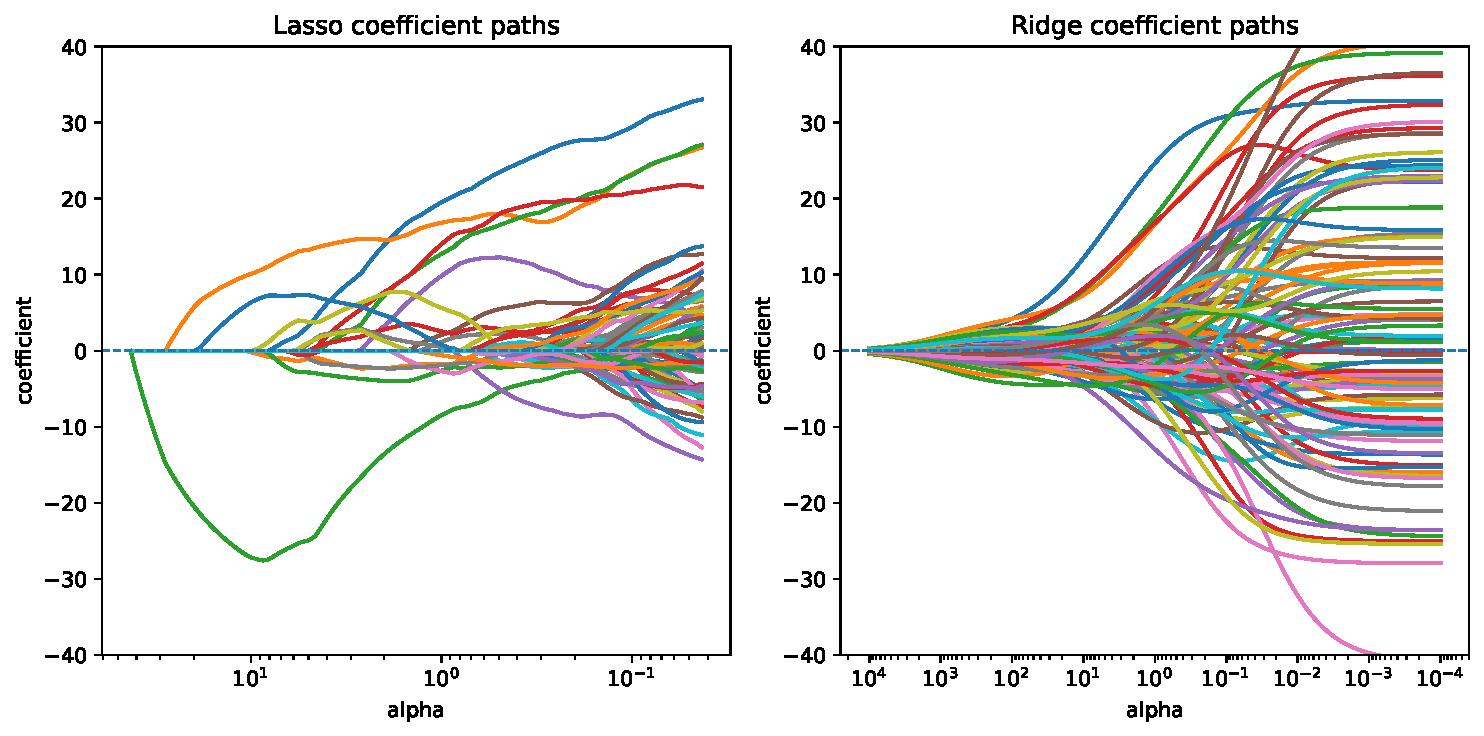
\includegraphics[keepaspectratio]{contents/1/shrinkage_files/figure-pdf/cell-23-output-1.pdf}}

\subsection{Tuning with
cross-validation}\label{tuning-with-cross-validation}

The choice of \texttt{alpha} strongly affects the fitted model.
Therefore in practice we usually tune it by cross-validation.

We first use \texttt{GridSearchCV} to select the best value of alpha.

\begin{Shaded}
\begin{Highlighting}[]
\ImportTok{from}\NormalTok{ sklearn.linear\_model }\ImportTok{import}\NormalTok{ Lasso}
\ImportTok{from}\NormalTok{ sklearn.model\_selection }\ImportTok{import}\NormalTok{ GridSearchCV}

\NormalTok{alphas }\OperatorTok{=}\NormalTok{ np.logspace(}\OperatorTok{{-}}\DecValTok{2}\NormalTok{, }\DecValTok{4}\NormalTok{, }\DecValTok{100}\NormalTok{)}

\NormalTok{lasso\_pipe }\OperatorTok{=}\NormalTok{ Pipeline(}
\NormalTok{    [}
\NormalTok{        (}\StringTok{"scaler"}\NormalTok{, StandardScaler()),}
\NormalTok{        (}\StringTok{"model"}\NormalTok{, Lasso(max\_iter}\OperatorTok{=}\DecValTok{100000}\NormalTok{, tol}\OperatorTok{=}\FloatTok{1e{-}3}\NormalTok{, random\_state}\OperatorTok{=}\DecValTok{0}\NormalTok{)),}
\NormalTok{    ]}
\NormalTok{)}

\NormalTok{lasso\_cv\_pipe }\OperatorTok{=}\NormalTok{ GridSearchCV(lasso\_pipe, param\_grid}\OperatorTok{=}\NormalTok{\{}\StringTok{"model\_\_alpha"}\NormalTok{: alphas\})}

\NormalTok{lasso\_cv\_pipe.fit(X\_train, y\_train)}
\NormalTok{y\_pred\_lasso\_cv }\OperatorTok{=}\NormalTok{ lasso\_cv\_pipe.predict(X\_test)}

\NormalTok{best\_alpha\_lasso }\OperatorTok{=}\NormalTok{ lasso\_cv\_pipe.best\_params\_[}\StringTok{"model\_\_alpha"}\NormalTok{]}

\BuiltInTok{print}\NormalTok{(}\StringTok{"Best lasso alpha:"}\NormalTok{, best\_alpha\_lasso)}
\BuiltInTok{print}\NormalTok{(}\StringTok{"Lasso Test MSE:"}\NormalTok{, mean\_squared\_error(y\_test, y\_pred\_lasso\_cv))}
\BuiltInTok{print}\NormalTok{(}\StringTok{"Lasso Test R\^{}2:"}\NormalTok{, r2\_score(y\_test, y\_pred\_lasso\_cv))}
\end{Highlighting}
\end{Shaded}

\begin{verbatim}
Best lasso alpha: 0.49770235643321115
Lasso Test MSE: 221.63625982655304
Lasso Test R^2: 0.9069993197512844
\end{verbatim}

For comparison, we tune ridge regression using the same cross-validation
procedure and \texttt{alpha} grid.

\begin{Shaded}
\begin{Highlighting}[]
\NormalTok{ridge\_cv\_pipe }\OperatorTok{=}\NormalTok{ Pipeline(}
\NormalTok{    [}
\NormalTok{        (}\StringTok{"scaler"}\NormalTok{, StandardScaler()),}
\NormalTok{        (}\StringTok{"model"}\NormalTok{, Ridge()),}
\NormalTok{    ]}
\NormalTok{)}

\NormalTok{ridge\_cv\_pipe }\OperatorTok{=}\NormalTok{ GridSearchCV(ridge\_cv\_pipe, param\_grid}\OperatorTok{=}\NormalTok{\{}\StringTok{"model\_\_alpha"}\NormalTok{: alphas\})}

\NormalTok{ridge\_cv\_pipe.fit(X\_train, y\_train)}
\NormalTok{y\_pred\_ridge\_cv }\OperatorTok{=}\NormalTok{ ridge\_cv\_pipe.predict(X\_test)}

\NormalTok{best\_alpha\_ridge }\OperatorTok{=}\NormalTok{ ridge\_cv\_pipe.best\_params\_[}\StringTok{"model\_\_alpha"}\NormalTok{]}

\BuiltInTok{print}\NormalTok{(}\StringTok{"Best ridge alpha:"}\NormalTok{, best\_alpha\_ridge)}
\BuiltInTok{print}\NormalTok{(}\StringTok{"Ridge Test MSE:"}\NormalTok{, mean\_squared\_error(y\_test, y\_pred\_ridge\_cv))}
\BuiltInTok{print}\NormalTok{(}\StringTok{"Ridge Test R\^{}2:"}\NormalTok{, r2\_score(y\_test, y\_pred\_ridge\_cv))}
\end{Highlighting}
\end{Shaded}

\begin{verbatim}
Best ridge alpha: 12.32846739442066
Ridge Test MSE: 280.8056227406724
Ridge Test R^2: 0.8821712929419413
\end{verbatim}

After obtaining the best regularization parameters, we mark them on the
coefficient path plots. This helps connect the selected model to the
whole regularization path.

\begin{Shaded}
\begin{Highlighting}[]
\ImportTok{import}\NormalTok{ numpy }\ImportTok{as}\NormalTok{ np}
\ImportTok{import}\NormalTok{ matplotlib.pyplot }\ImportTok{as}\NormalTok{ plt}
\ImportTok{from}\NormalTok{ sklearn.linear\_model }\ImportTok{import}\NormalTok{ lasso\_path, Ridge}
\ImportTok{from}\NormalTok{ sklearn.preprocessing }\ImportTok{import}\NormalTok{ StandardScaler}

\NormalTok{scaler }\OperatorTok{=}\NormalTok{ StandardScaler()}
\NormalTok{X\_train\_scaled }\OperatorTok{=}\NormalTok{ scaler.fit\_transform(X\_train)}

\NormalTok{fig, axs }\OperatorTok{=}\NormalTok{ plt.subplots(}\DecValTok{1}\NormalTok{, }\DecValTok{2}\NormalTok{, figsize}\OperatorTok{=}\NormalTok{(}\DecValTok{10}\NormalTok{, }\DecValTok{5}\NormalTok{))}


\NormalTok{alphas\_lasso, coefs\_lasso, \_ }\OperatorTok{=}\NormalTok{ lasso\_path(X\_train\_scaled, y\_train)}

\NormalTok{axs[}\DecValTok{0}\NormalTok{].plot(alphas\_lasso, coefs\_lasso.T)}
\NormalTok{axs[}\DecValTok{0}\NormalTok{].axvline(}
\NormalTok{    best\_alpha\_lasso, linestyle}\OperatorTok{=}\StringTok{"{-}{-}"}\NormalTok{, color}\OperatorTok{=}\StringTok{"black"}\NormalTok{, label}\OperatorTok{=}\StringTok{"selected alpha"}
\NormalTok{)}
\NormalTok{axs[}\DecValTok{0}\NormalTok{].set\_title(}\StringTok{"Lasso coefficient paths"}\NormalTok{)}

\NormalTok{alphas\_ridge }\OperatorTok{=}\NormalTok{ np.logspace(}\OperatorTok{{-}}\DecValTok{4}\NormalTok{, }\DecValTok{4}\NormalTok{, }\DecValTok{100}\NormalTok{)}
\NormalTok{coefs\_ridge }\OperatorTok{=}\NormalTok{ []}

\ControlFlowTok{for}\NormalTok{ a }\KeywordTok{in}\NormalTok{ alphas\_ridge:}
\NormalTok{    ridge }\OperatorTok{=}\NormalTok{ Ridge(alpha}\OperatorTok{=}\NormalTok{a)}
\NormalTok{    ridge.fit(X\_train\_scaled, y\_train)}
\NormalTok{    coefs\_ridge.append(ridge.coef\_)}

\NormalTok{coefs\_ridge }\OperatorTok{=}\NormalTok{ np.array(coefs\_ridge)}

\NormalTok{axs[}\DecValTok{1}\NormalTok{].plot(alphas\_ridge, coefs\_ridge)}
\NormalTok{axs[}\DecValTok{1}\NormalTok{].axvline(}
\NormalTok{    best\_alpha\_ridge, linestyle}\OperatorTok{=}\StringTok{"{-}{-}"}\NormalTok{, color}\OperatorTok{=}\StringTok{"black"}\NormalTok{, label}\OperatorTok{=}\StringTok{"selected alpha"}
\NormalTok{)}
\NormalTok{axs[}\DecValTok{1}\NormalTok{].set\_title(}\StringTok{"Ridge coefficient paths"}\NormalTok{)}

\ControlFlowTok{for}\NormalTok{ ax }\KeywordTok{in}\NormalTok{ axs:}
\NormalTok{    ax.set\_xscale(}\StringTok{"log"}\NormalTok{)}
\NormalTok{    ax.axhline(}\DecValTok{0}\NormalTok{, linestyle}\OperatorTok{=}\StringTok{"{-}{-}"}\NormalTok{, linewidth}\OperatorTok{=}\DecValTok{1}\NormalTok{)}
\NormalTok{    ax.invert\_xaxis()}
\NormalTok{    ax.set\_ylim(}\OperatorTok{{-}}\DecValTok{40}\NormalTok{, }\DecValTok{40}\NormalTok{)}
\NormalTok{    ax.set\_xlabel(}\StringTok{"alpha"}\NormalTok{)}
\NormalTok{    ax.set\_ylabel(}\StringTok{"coefficient"}\NormalTok{)}

\NormalTok{plt.tight\_layout()}
\end{Highlighting}
\end{Shaded}

\pandocbounded{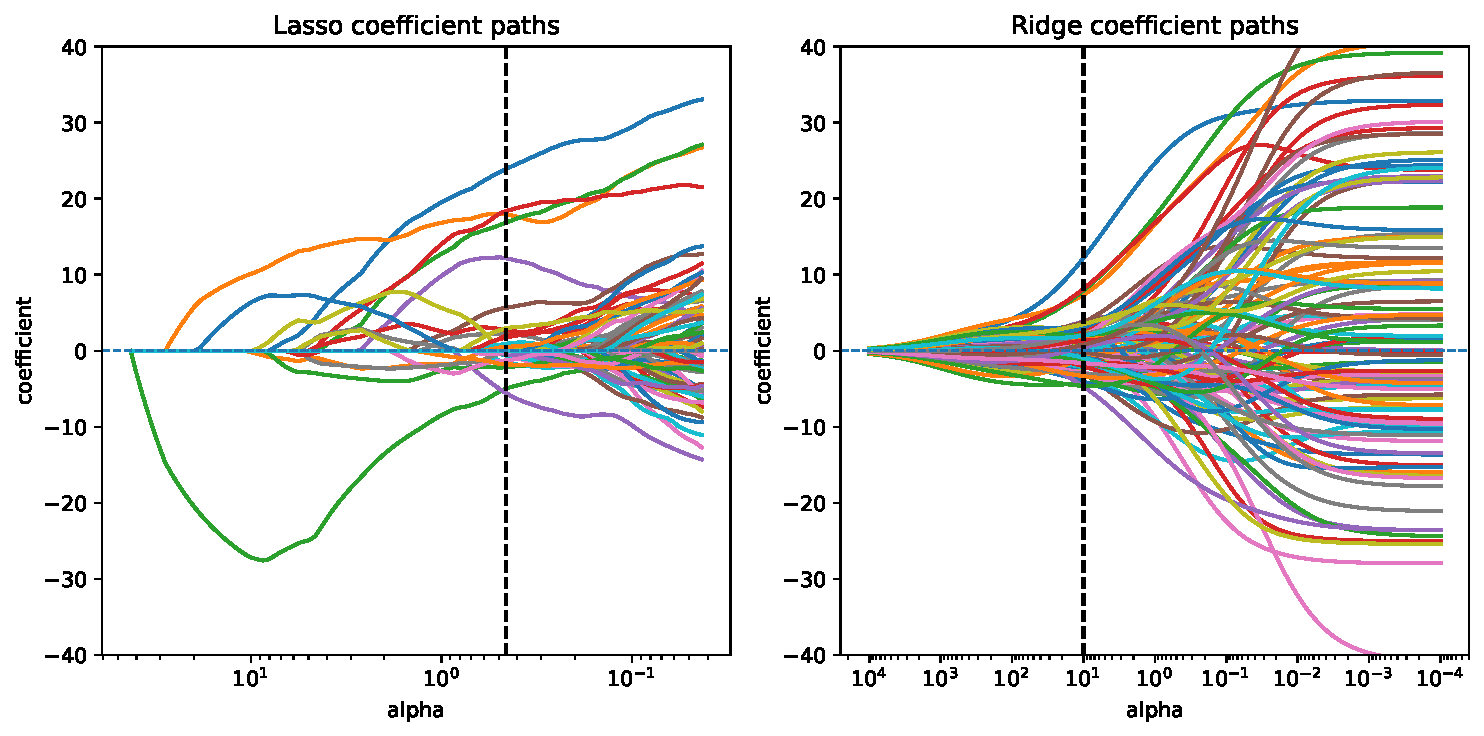
\includegraphics[keepaspectratio]{contents/1/shrinkage_files/figure-pdf/cell-26-output-1.pdf}}

\begin{tcolorbox}[enhanced jigsaw, arc=.35mm, bottomrule=.15mm, bottomtitle=1mm, breakable, colback=white, colbacktitle=quarto-callout-caution-color!10!white, colframe=quarto-callout-caution-color-frame, coltitle=black, left=2mm, leftrule=.75mm, opacityback=0, opacitybacktitle=0.6, rightrule=.15mm, title=\textcolor{quarto-callout-caution-color}{\faFire}\hspace{0.5em}{Data leaks in \texttt{LassoCV}}, titlerule=0mm, toprule=.15mm, toptitle=1mm]

When using a pipeline such as
\texttt{StandardScaler-\textgreater{}LassoCV}, the
\texttt{StandardScaler} is fitted once using the entire training set
before \texttt{LassoCV} performs its internal cross-validation. As a
result, the validation folds inside \texttt{LassoCV} are evaluated on
data that were standardized using information from all training
observations, including observations outside the current fold.

This introduces a small amount of data leakage and may make the
cross-validation estimate slightly optimistic.

A safer approach is to place the entire pipeline inside
\texttt{GridSearchCV} using \texttt{Lasso} instead of \texttt{LassoCV}.
In this setup, the scaler is refit separately within each training fold,
preventing leakage.

\texttt{LassoCV} is still useful when no preprocessing pipeline is
involved, and it is often faster than \texttt{GridSearchCV} because of
its specialized implementation.

Similarly, \texttt{RidgeCV} may suffer from the same issue when placed
after preprocessing steps in a pipeline. However, when \texttt{cv=None},
\texttt{RidgeCV} uses formulas to estimate the LOOCV. In practice, the
resulting bias is often small, so many users accept this shortcut for
convenience and speed.

\end{tcolorbox}

\subsection{Validation curves}\label{validation-curves}

Another way to visualize tuning is through the validation curve. Here we
plot the mean training and validation scores across the same grid of
\texttt{alpha} values used above. The score is negative MSE, so higher
values are better.

\begin{itemize}
\tightlist
\item
  When \texttt{alpha} is too small, the model may overfit.
\item
  When \texttt{alpha} is too large, the model may underfit.
\item
  A good value of \texttt{alpha} balances these two effects.
\end{itemize}

\begin{Shaded}
\begin{Highlighting}[]
\ImportTok{from}\NormalTok{ sklearn.model\_selection }\ImportTok{import}\NormalTok{ validation\_curve}
\ImportTok{from}\NormalTok{ sklearn.pipeline }\ImportTok{import}\NormalTok{ Pipeline}
\ImportTok{from}\NormalTok{ sklearn.preprocessing }\ImportTok{import}\NormalTok{ StandardScaler}
\ImportTok{from}\NormalTok{ sklearn.linear\_model }\ImportTok{import}\NormalTok{ Ridge, Lasso}
\ImportTok{import}\NormalTok{ numpy }\ImportTok{as}\NormalTok{ np}
\ImportTok{import}\NormalTok{ matplotlib.pyplot }\ImportTok{as}\NormalTok{ plt}

\NormalTok{fig, axs }\OperatorTok{=}\NormalTok{ plt.subplots(}\DecValTok{1}\NormalTok{, }\DecValTok{2}\NormalTok{, figsize}\OperatorTok{=}\NormalTok{(}\DecValTok{10}\NormalTok{, }\FloatTok{4.5}\NormalTok{))}

\NormalTok{lasso\_pipe }\OperatorTok{=}\NormalTok{ Pipeline(}
\NormalTok{    [}
\NormalTok{        (}\StringTok{"scaler"}\NormalTok{, StandardScaler()),}
\NormalTok{        (}\StringTok{"model"}\NormalTok{, Lasso(max\_iter}\OperatorTok{=}\DecValTok{100000}\NormalTok{, tol}\OperatorTok{=}\FloatTok{1e{-}3}\NormalTok{, random\_state}\OperatorTok{=}\DecValTok{0}\NormalTok{)),}
\NormalTok{    ]}
\NormalTok{)}

\NormalTok{train\_scores\_lasso, test\_scores\_lasso }\OperatorTok{=}\NormalTok{ validation\_curve(}
\NormalTok{    lasso\_pipe, X\_train, y\_train, param\_name}\OperatorTok{=}\StringTok{"model\_\_alpha"}\NormalTok{, param\_range}\OperatorTok{=}\NormalTok{alphas}
\NormalTok{)}

\NormalTok{axs[}\DecValTok{0}\NormalTok{].plot(alphas, train\_scores\_lasso.mean(axis}\OperatorTok{=}\DecValTok{1}\NormalTok{), label}\OperatorTok{=}\StringTok{"train"}\NormalTok{)}
\NormalTok{axs[}\DecValTok{0}\NormalTok{].plot(alphas, test\_scores\_lasso.mean(axis}\OperatorTok{=}\DecValTok{1}\NormalTok{), label}\OperatorTok{=}\StringTok{"test"}\NormalTok{)}
\NormalTok{axs[}\DecValTok{0}\NormalTok{].axvline(best\_alpha\_lasso, color}\OperatorTok{=}\StringTok{"black"}\NormalTok{, linestyle}\OperatorTok{=}\StringTok{"{-}{-}"}\NormalTok{, label}\OperatorTok{=}\StringTok{"best alpha"}\NormalTok{)}
\NormalTok{axs[}\DecValTok{0}\NormalTok{].set\_title(}\StringTok{"Validation curve for lasso"}\NormalTok{)}


\NormalTok{ridge\_pipe }\OperatorTok{=}\NormalTok{ Pipeline(}
\NormalTok{    [}
\NormalTok{        (}\StringTok{"scaler"}\NormalTok{, StandardScaler()),}
\NormalTok{        (}\StringTok{"model"}\NormalTok{, Ridge()),}
\NormalTok{    ]}
\NormalTok{)}

\NormalTok{train\_scores\_ridge, test\_scores\_ridge }\OperatorTok{=}\NormalTok{ validation\_curve(}
\NormalTok{    ridge\_pipe, X\_train, y\_train, param\_name}\OperatorTok{=}\StringTok{"model\_\_alpha"}\NormalTok{, param\_range}\OperatorTok{=}\NormalTok{alphas}
\NormalTok{)}

\NormalTok{axs[}\DecValTok{1}\NormalTok{].plot(alphas, train\_scores\_ridge.mean(axis}\OperatorTok{=}\DecValTok{1}\NormalTok{), label}\OperatorTok{=}\StringTok{"train"}\NormalTok{)}
\NormalTok{axs[}\DecValTok{1}\NormalTok{].plot(alphas, test\_scores\_ridge.mean(axis}\OperatorTok{=}\DecValTok{1}\NormalTok{), label}\OperatorTok{=}\StringTok{"test"}\NormalTok{)}
\NormalTok{axs[}\DecValTok{1}\NormalTok{].axvline(best\_alpha\_ridge, color}\OperatorTok{=}\StringTok{"black"}\NormalTok{, linestyle}\OperatorTok{=}\StringTok{"{-}{-}"}\NormalTok{, label}\OperatorTok{=}\StringTok{"best alpha"}\NormalTok{)}
\NormalTok{axs[}\DecValTok{1}\NormalTok{].set\_title(}\StringTok{"Validation curve for ridge"}\NormalTok{)}


\ControlFlowTok{for}\NormalTok{ ax }\KeywordTok{in}\NormalTok{ axs:}
\NormalTok{    ax.set\_xscale(}\StringTok{"log"}\NormalTok{)}
\NormalTok{    ax.set\_xlabel(}\StringTok{"alpha"}\NormalTok{)}
\NormalTok{    ax.set\_ylabel(}\VerbatimStringTok{r"score: }\DecValTok{$}\VerbatimStringTok{R}\DecValTok{\^{}}\VerbatimStringTok{2}\DecValTok{$}\VerbatimStringTok{"}\NormalTok{)}
\NormalTok{    ax.legend()}

\NormalTok{plt.tight\_layout()}
\end{Highlighting}
\end{Shaded}

\pandocbounded{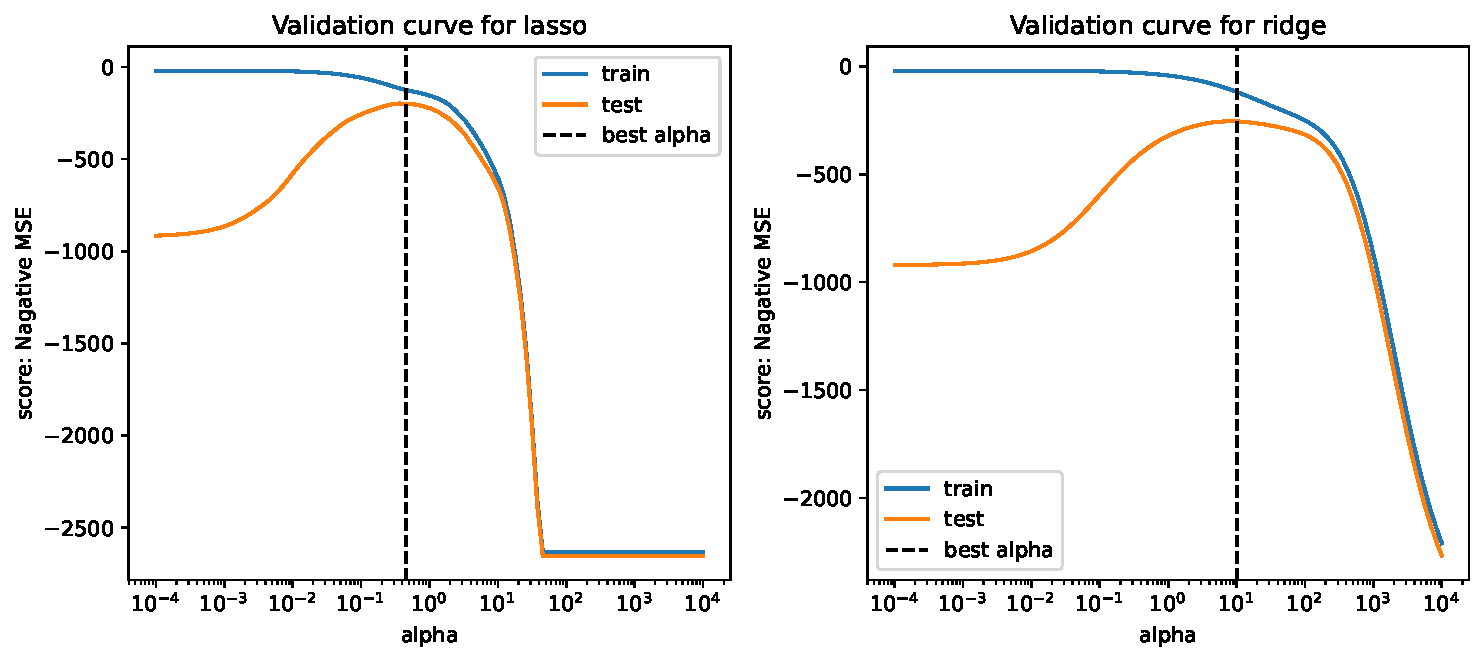
\includegraphics[keepaspectratio]{contents/1/shrinkage_files/figure-pdf/cell-27-output-1.pdf}}

\section{Elastic net}\label{elastic-net}

Elastic net combines the \(L_1\) penalty of lasso and the \(L_2\)
penalty of ridge regression. It is useful when we want a sparse model,
but the predictors are strongly correlated.

\begin{definition}[Elastic
net]\protect\hypertarget{def-elastic-net}{}\label{def-elastic-net}

The elastic net estimator is defined by

\[
\hat{\beta}_{\text{EN}}
=
\arg\min_{\beta}
\qty{
\norm{y-X\beta}_2^2
+
\lambda\qty[
\alpha\norm{\beta}_1
+
(1-\alpha)\norm{\beta}_2^2
]
},
\]

where \(\lambda \ge 0\) controls the overall regularization strength and
\(0 \le \alpha \le 1\) controls the mixture of the two penalties.

\end{definition}

\begin{itemize}
\tightlist
\item
  When \(\alpha=1\), elastic net reduces to lasso.
\item
  When \(\alpha=0\), elastic net reduces to ridge regression.
\item
  The \(L_1\) penalty can set coefficients exactly to zero, while the
  \(L_2\) penalty improves stability when predictors are strongly
  correlated.
\end{itemize}

\begin{tcolorbox}[enhanced jigsaw, arc=.35mm, bottomrule=.15mm, bottomtitle=1mm, breakable, colback=white, colbacktitle=quarto-callout-note-color!10!white, colframe=quarto-callout-note-color-frame, coltitle=black, left=2mm, leftrule=.75mm, opacityback=0, opacitybacktitle=0.6, rightrule=.15mm, title=\textcolor{quarto-callout-note-color}{\faInfo}\hspace{0.5em}{Grouping effect}, titlerule=0mm, toprule=.15mm, toptitle=1mm]

An important feature of elastic net is the \textbf{grouping effect}.
When several predictors are strongly correlated, lasso may select only
one of them, and the selected predictor may change substantially across
different samples. In contrast, the \(L_2\) component of elastic net
encourages correlated predictors to have similar coefficients, so they
tend to enter or leave the model together.

Elastic net therefore combines variable selection with more stable
coefficient estimates when predictors are strongly correlated.

\end{tcolorbox}

\subsection{Elastic net in Python}\label{elastic-net-in-python}

In \texttt{sklearn}, elastic net is implemented by \texttt{ElasticNet}.
The parameter names are slightly confusing:

\begin{itemize}
\tightlist
\item
  \texttt{alpha} corresponds to \(\lambda\), the overall regularization
  strength.
\item
  \texttt{l1\_ratio} corresponds to \(\alpha\), the mixture of the
  \(L_1\) and \(L_2\) penalties.
\end{itemize}

Thus, \texttt{l1\_ratio=1} gives lasso, while values closer to \(0\)
behave more like ridge regression.

\begin{Shaded}
\begin{Highlighting}[]
\ImportTok{from}\NormalTok{ sklearn.linear\_model }\ImportTok{import}\NormalTok{ ElasticNet}

\NormalTok{en }\OperatorTok{=}\NormalTok{ ElasticNet(alpha}\OperatorTok{=}\FloatTok{0.1}\NormalTok{, l1\_ratio}\OperatorTok{=}\FloatTok{0.5}\NormalTok{, max\_iter}\OperatorTok{=}\DecValTok{10000}\NormalTok{)}
\NormalTok{en.fit(X\_train, y\_train)}
\NormalTok{y\_pred\_en }\OperatorTok{=}\NormalTok{ en.predict(X\_test)}
\end{Highlighting}
\end{Shaded}

\subsection{\texorpdfstring{Choosing \(\alpha\) and
\(\lambda\)}{Choosing \textbackslash alpha and \textbackslash lambda}}\label{choosing-alpha-and-lambda}

Both parameters can be selected using \texttt{ElasticNetCV}.

\begin{Shaded}
\begin{Highlighting}[]
\ImportTok{from}\NormalTok{ sklearn.linear\_model }\ImportTok{import}\NormalTok{ ElasticNetCV}

\NormalTok{en\_cv }\OperatorTok{=}\NormalTok{ ElasticNetCV(}
\NormalTok{    l1\_ratio}\OperatorTok{=}\NormalTok{[}\FloatTok{0.1}\NormalTok{, }\FloatTok{0.5}\NormalTok{, }\FloatTok{0.9}\NormalTok{, }\FloatTok{1.0}\NormalTok{],}
\NormalTok{    alphas}\OperatorTok{=}\NormalTok{np.logspace(}\OperatorTok{{-}}\DecValTok{4}\NormalTok{, }\DecValTok{4}\NormalTok{, }\DecValTok{100}\NormalTok{),}
\NormalTok{    cv}\OperatorTok{=}\DecValTok{5}\NormalTok{,}
\NormalTok{    max\_iter}\OperatorTok{=}\DecValTok{10000}\NormalTok{,}
\NormalTok{).fit(X\_train, y\_train)}
\end{Highlighting}
\end{Shaded}

As noted in the \hyperref[caution-cv-preprocessing-leakage]{earlier
caution}, preprocessing should be performed separately within each fold.
Therefore, we use \texttt{GridSearchCV} with \texttt{ElasticNet} instead
of a \texttt{StandardScaler}--\texttt{ElasticNetCV} pipeline.

\begin{Shaded}
\begin{Highlighting}[]
\ImportTok{import}\NormalTok{ numpy }\ImportTok{as}\NormalTok{ np}
\ImportTok{from}\NormalTok{ sklearn.model\_selection }\ImportTok{import}\NormalTok{ GridSearchCV}
\ImportTok{from}\NormalTok{ sklearn.pipeline }\ImportTok{import}\NormalTok{ make\_pipeline}
\ImportTok{from}\NormalTok{ sklearn.preprocessing }\ImportTok{import}\NormalTok{ StandardScaler}

\NormalTok{en\_pipe }\OperatorTok{=}\NormalTok{ make\_pipeline(}
\NormalTok{    StandardScaler(),}
\NormalTok{    ElasticNet(max\_iter}\OperatorTok{=}\DecValTok{100000}\NormalTok{, tol}\OperatorTok{=}\FloatTok{1e{-}3}\NormalTok{),}
\NormalTok{)}

\NormalTok{alphas }\OperatorTok{=}\NormalTok{ np.logspace(}\OperatorTok{{-}}\DecValTok{2}\NormalTok{, }\DecValTok{4}\NormalTok{, }\DecValTok{100}\NormalTok{)}

\NormalTok{en\_grid }\OperatorTok{=}\NormalTok{ GridSearchCV(}
\NormalTok{    en\_pipe,}
\NormalTok{    \{}
        \StringTok{"elasticnet\_\_alpha"}\NormalTok{: alphas,}
        \StringTok{"elasticnet\_\_l1\_ratio"}\NormalTok{: [}\FloatTok{0.1}\NormalTok{, }\FloatTok{0.5}\NormalTok{, }\FloatTok{0.9}\NormalTok{, }\FloatTok{1.0}\NormalTok{],}
\NormalTok{    \},}
\NormalTok{)}
\NormalTok{en\_grid.fit(X\_train, y\_train)}

\NormalTok{y\_pred\_en }\OperatorTok{=}\NormalTok{ en\_grid.predict(X\_test)}

\BuiltInTok{print}\NormalTok{(}\StringTok{"Best lambda:"}\NormalTok{, en\_grid.best\_params\_[}\StringTok{"elasticnet\_\_alpha"}\NormalTok{])}
\BuiltInTok{print}\NormalTok{(}\StringTok{"Best alpha :"}\NormalTok{, en\_grid.best\_params\_[}\StringTok{"elasticnet\_\_l1\_ratio"}\NormalTok{])}
\BuiltInTok{print}\NormalTok{(}\StringTok{"Test MSE   :"}\NormalTok{, mean\_squared\_error(y\_test, y\_pred\_en))}
\BuiltInTok{print}\NormalTok{(}\StringTok{"Test R\^{}2   :"}\NormalTok{, r2\_score(y\_test, y\_pred\_en))}
\end{Highlighting}
\end{Shaded}

\begin{verbatim}
Best lambda: 0.49770235643321115
Best alpha : 1.0
Test MSE   : 221.63625982655304
Test R^2   : 0.9069993197512844
\end{verbatim}

\subsection{Summary}\label{summary}

Finally, we summarize the test performance and the number of nonzero
coefficients for each model.

\begin{Shaded}
\begin{Highlighting}[]
\ImportTok{import}\NormalTok{ pandas }\ImportTok{as}\NormalTok{ pd}

\NormalTok{results }\OperatorTok{=}\NormalTok{ []}

\NormalTok{models }\OperatorTok{=}\NormalTok{ \{}
    \StringTok{"OLS"}\NormalTok{: ols\_pipe,}
    \StringTok{"Ridge"}\NormalTok{: ridge\_cv\_pipe,}
    \StringTok{"Lasso"}\NormalTok{: lasso\_cv\_pipe,}
    \StringTok{"Elastic Net"}\NormalTok{: en\_grid,}
\NormalTok{\}}

\ControlFlowTok{for}\NormalTok{ name, model }\KeywordTok{in}\NormalTok{ models.items():}
\NormalTok{    y\_pred }\OperatorTok{=}\NormalTok{ model.predict(X\_test)}
\NormalTok{    mse }\OperatorTok{=}\NormalTok{ mean\_squared\_error(y\_test, y\_pred)}
\NormalTok{    r2 }\OperatorTok{=}\NormalTok{ r2\_score(y\_test, y\_pred)}

\NormalTok{    fitted\_pipe }\OperatorTok{=}\NormalTok{ (}
\NormalTok{        model.best\_estimator\_}
        \ControlFlowTok{if}\NormalTok{ name }\KeywordTok{in}\NormalTok{ [}\StringTok{"Ridge"}\NormalTok{, }\StringTok{"Lasso"}\NormalTok{, }\StringTok{"Elastic Net"}\NormalTok{]}
        \ControlFlowTok{else}\NormalTok{ model}
\NormalTok{    )}
\NormalTok{    model\_step }\OperatorTok{=} \StringTok{"elasticnet"} \ControlFlowTok{if}\NormalTok{ name }\OperatorTok{==} \StringTok{"Elastic Net"} \ControlFlowTok{else} \StringTok{"model"}
\NormalTok{    fitted\_model }\OperatorTok{=}\NormalTok{ fitted\_pipe.named\_steps[model\_step]}
\NormalTok{    n\_nonzero }\OperatorTok{=}\NormalTok{ np.}\BuiltInTok{sum}\NormalTok{(fitted\_model.coef\_ }\OperatorTok{!=} \DecValTok{0}\NormalTok{)}

    \ControlFlowTok{if}\NormalTok{ name }\OperatorTok{==} \StringTok{"Lasso"}\NormalTok{:}
\NormalTok{        alpha }\OperatorTok{=}\NormalTok{ model.best\_params\_[}\StringTok{"model\_\_alpha"}\NormalTok{]}
\NormalTok{        l1\_ratio }\OperatorTok{=} \FloatTok{1.0}
    \ControlFlowTok{elif}\NormalTok{ name }\OperatorTok{==} \StringTok{"Elastic Net"}\NormalTok{:}
\NormalTok{        alpha }\OperatorTok{=}\NormalTok{ model.best\_params\_[}\StringTok{"elasticnet\_\_alpha"}\NormalTok{]}
\NormalTok{        l1\_ratio }\OperatorTok{=}\NormalTok{ model.best\_params\_[}\StringTok{"elasticnet\_\_l1\_ratio"}\NormalTok{]}
    \ControlFlowTok{elif}\NormalTok{ name }\OperatorTok{==} \StringTok{"Ridge"}\NormalTok{:}
\NormalTok{        alpha }\OperatorTok{=}\NormalTok{ model.best\_params\_[}\StringTok{"model\_\_alpha"}\NormalTok{]}
\NormalTok{        l1\_ratio }\OperatorTok{=} \FloatTok{0.0}
    \ControlFlowTok{else}\NormalTok{:}
\NormalTok{        alpha }\OperatorTok{=} \VariableTok{None}
\NormalTok{        l1\_ratio }\OperatorTok{=} \VariableTok{None}

\NormalTok{    results.append(\{}
        \StringTok{\textquotesingle{}Model\textquotesingle{}}\NormalTok{: name,}
        \StringTok{\textquotesingle{}Best alpha\textquotesingle{}}\NormalTok{: alpha,}
        \StringTok{\textquotesingle{}L1 ratio\textquotesingle{}}\NormalTok{: l1\_ratio,}
        \StringTok{\textquotesingle{}Test MSE\textquotesingle{}}\NormalTok{: mse,}
        \StringTok{\textquotesingle{}Test R\^{}2\textquotesingle{}}\NormalTok{: r2,}
        \StringTok{\textquotesingle{}Nonzero coefs\textquotesingle{}}\NormalTok{: n\_nonzero}
\NormalTok{    \})}

\NormalTok{pd.DataFrame(results)}
\end{Highlighting}
\end{Shaded}

{\def\LTcaptype{none} % do not increment counter
\begin{longtable}[]{@{}lllllll@{}}
\toprule\noalign{}
& Model & Best alpha & L1 ratio & Test MSE & Test R\^{}2 & Nonzero
coefs \\
\midrule\noalign{}
\endhead
\bottomrule\noalign{}
\endlastfoot
0 & OLS & NaN & NaN & 1212.515486 & 0.491217 & 100 \\
1 & Ridge & 12.328467 & 0.0 & 280.805623 & 0.882171 & 100 \\
2 & Lasso & 0.497702 & 1.0 & 221.636260 & 0.906999 & 27 \\
3 & Elastic Net & 0.497702 & 1.0 & 221.636260 & 0.906999 & 27 \\
\end{longtable}
}

This example shows the main practical differences among ridge, lasso,
and elastic net:

\begin{itemize}
\tightlist
\item
  Ridge shrinks coefficients continuously and is especially useful when
  predictors are strongly correlated.
\item
  Lasso also shrinks coefficients, but can force some of them to be
  exactly zero, producing a sparse model.
\item
  Elastic net combines both penalties, balancing sparsity with greater
  stability among correlated predictors. In this example, however,
  cross-validation selects \texttt{l1\_ratio=1}, so the fitted elastic
  net model reduces to lasso.
\end{itemize}

In high-dimensional settings with collinearity and only a subset of
truly relevant predictors, lasso can provide a more interpretable sparse
model, ridge can produce more stable coefficient estimates, and elastic
net offers a data-driven compromise between the two.

\begin{tcolorbox}[enhanced jigsaw, arc=.35mm, bottomrule=.15mm, bottomtitle=1mm, breakable, colback=white, colbacktitle=quarto-callout-note-color!10!white, colframe=quarto-callout-note-color-frame, coltitle=black, left=2mm, leftrule=.75mm, opacityback=0, opacitybacktitle=0.6, rightrule=.15mm, title=\textcolor{quarto-callout-note-color}{\faInfo}\hspace{0.5em}{Note}, titlerule=0mm, toprule=.15mm, toptitle=1mm]

In this example, the best \texttt{l1\_ratio} is 1. This is likely
because the true model is sparse: only a small number of predictors
contribute directly to the response, making variable selection
especially useful. Thus, although the predictors are strongly
correlated, the additional ridge penalty does not improve
cross-validation performance for this particular dataset.

\end{tcolorbox}

\chapter{Dimension reduction}\label{dimension-reduction}

When the number of predictors is large or when predictors are highly
correlated, directly fitting a regression model using the original
predictors may lead to unstable estimates and poor predictive
performance.

One approach to address this problem is dimension reduction. Instead of
using the original predictors directly, we first construct a smaller
number of derived variables (called components) and then perform
regression using these components.

Two commonly used methods are

\begin{itemize}
\tightlist
\item
  Principal Component Regression (PCR)
\item
  Partial Least Squares (PLS)
\end{itemize}

Both methods construct new variables that are linear combinations of the
original predictors, but they differ in how those combinations are
chosen.

\section{Principal Component Regression
(PCR)}\label{principal-component-regression-pcr}

PCR first applies principal component analysis (PCA) to the predictor
matrix \(X\), and then uses the leading principal components as
predictors in a regression model.

The key idea is that most of the variation in the predictors often lies
in a lower-dimensional subspace.

\begin{definition}[Principal Component
Regression]\protect\hypertarget{def-pcr}{}\label{def-pcr}

Let \(X\) be the \(n \times p\) predictor matrix.

The principal components are defined as

\[
Z_k = X v_k,
\]

where \(v_k\) is the \(k\)-th eigenvector of the Gram matrix
\(X^\top X\).

Principal component regression fits a linear model using the first \(m\)
components:

\[
y = \theta_0 + \theta_1 Z_1 + \theta_2 Z_2 + \cdots + \theta_m Z_m + \varepsilon.
\]

Here

\begin{itemize}
\tightlist
\item
  \(Z_1,\ldots,Z_m\) are the first \(m\) principal components
\item
  \(m < p\) is chosen by cross-validation
\end{itemize}

\end{definition}

Thus PCR replaces the original predictors with a smaller set of
orthogonal components.

\begin{tcolorbox}[enhanced jigsaw, arc=.35mm, bottomrule=.15mm, bottomtitle=1mm, breakable, colback=white, colbacktitle=quarto-callout-note-color!10!white, colframe=quarto-callout-note-color-frame, coltitle=black, left=2mm, leftrule=.75mm, opacityback=0, opacitybacktitle=0.6, rightrule=.15mm, title=\textcolor{quarto-callout-note-color}{\faInfo}\hspace{0.5em}{Key feature of PCR}, titlerule=0mm, toprule=.15mm, toptitle=1mm]

PCR constructs components using only the predictor matrix \(X\), without
considering the response \(y\).

As a result, the directions that explain the most variation in \(X\) are
not necessarily the directions that are most predictive of \(y\).

\end{tcolorbox}

\subsection{Data matrix and its geometric
views}\label{data-matrix-and-its-geometric-views}

Let \(X \in \mathbb{R}^{n \times p}\) be a data matrix with \(n\)
observations and \(p\) predictors. We assume columns are centered
(\(\sum_{i=1}^n x_{ij} = 0\)) so that the origin represents the sample
mean.

\textbf{Column (variable) view: observation space \(\mathbb{R}^n\)}

Each column of \(X_j\) is a vector in \(n\)-dimensional space, which
represents one predictor across all observations.

\begin{itemize}
\tightlist
\item
  This space is often called the observation space.
\item
  Geometry in this space describes relationships between predictors:

  \begin{itemize}
  \tightlist
  \item
    Inner products encode covariance.
  \item
    After standardization, angles encode correlation.
  \item
    Orthogonality corresponds to zero correlation.
  \end{itemize}
\end{itemize}

\textbf{Row (observation) view: feature space \(\mathbb{R}^p\)}

Each row of \(x_i^\top\) is a vector in \(p\)-dimensional space, which
represents one observation across all predictors.

\begin{itemize}
\tightlist
\item
  This space is called the feature space.
\item
  Geometry in this space describes relationships between observations:

  \begin{itemize}
  \tightlist
  \item
    Euclidean distance measures dissimilarity.
  \item
    Clustering and nearest-neighbor methods operate in this space.
  \end{itemize}
\end{itemize}

\begin{example}[]\protect\hypertarget{exm-}{}\label{exm-}

~

Click to expand.

To demonstrate the idea, we generate the following dataset. It contains
2 variables.

\begin{Shaded}
\begin{Highlighting}[]
\ImportTok{import}\NormalTok{ numpy }\ImportTok{as}\NormalTok{ np}
\ImportTok{import}\NormalTok{ matplotlib.pyplot }\ImportTok{as}\NormalTok{ plt}

\NormalTok{rng }\OperatorTok{=}\NormalTok{ np.random.default\_rng(}\DecValTok{0}\NormalTok{)}

\NormalTok{n }\OperatorTok{=} \DecValTok{100}

\NormalTok{Sigma }\OperatorTok{=}\NormalTok{ np.array([[}\FloatTok{0.5}\NormalTok{, }\OperatorTok{{-}}\FloatTok{0.65}\NormalTok{], [}\OperatorTok{{-}}\FloatTok{0.65}\NormalTok{, }\FloatTok{1.0}\NormalTok{]])}
\NormalTok{mu }\OperatorTok{=}\NormalTok{ np.array([}\DecValTok{1}\NormalTok{, }\DecValTok{2}\NormalTok{])}

\NormalTok{X }\OperatorTok{=}\NormalTok{ rng.multivariate\_normal(mean}\OperatorTok{=}\NormalTok{mu, cov}\OperatorTok{=}\NormalTok{Sigma, size}\OperatorTok{=}\NormalTok{n)}

\NormalTok{plt.scatter(X[:, }\DecValTok{0}\NormalTok{], X[:, }\DecValTok{1}\NormalTok{])}

\NormalTok{plt.xlabel(}\StringTok{"x1"}\NormalTok{)}
\NormalTok{plt.ylabel(}\StringTok{"x2"}\NormalTok{)}\OperatorTok{;}
\end{Highlighting}
\end{Shaded}

\pandocbounded{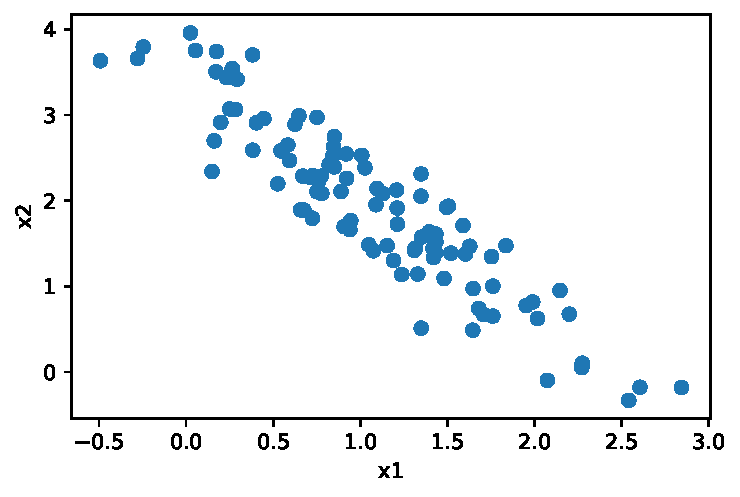
\includegraphics[keepaspectratio]{contents/1/dr_files/figure-pdf/cell-2-output-1.pdf}}

Each point is an observation and is represented by a point in the
feature space.

\end{example}

\begin{center}\rule{0.5\linewidth}{0.5pt}\end{center}

\subsection{Singular Value Decomposition
(SVD)}\label{singular-value-decomposition-svd}

The SVD provides the most direct link between the two geometric
perspectives.

For a matrix with \(\text{rank}(X) = r\) \[
X = U D V^\top,
\] where

\begin{itemize}
\tightlist
\item
  \(U \in \mathbb{R}^{n \times r}\), \(U^\top U = I\)
\item
  \(D = \operatorname{diag}(d_1,\dots,d_r)\),
  \(d_1 \ge \cdots \ge d_r > 0\)
\item
  \(V \in \mathbb{R}^{p \times r}\), \(V^\top V = I\)
\end{itemize}

\begin{center}\rule{0.5\linewidth}{0.5pt}\end{center}

\subsection{Principal components (PC)}\label{principal-components-pc}

Principal component analysis (PCA) constructs new variables as linear
combinations of the original predictors. It builds upon SVD.

Let \(Z =XV=UD= \qty[Z_1, \dots, Z_r]=\mqty[z_{ij}]\) denote the
principal components. Each principal component has the form \[
Z_j = X v_j=v_{1j}X_1+v_{2j}X_2+\ldots+v_{pj}X_p
\] where \(v_j=\mqty[v_{1j}&\ldots&v_{pj}]^{\top} \in \mathbb{R}^p\) is
a unit vector.

\textbf{Loadings (directions)}

\begin{itemize}
\tightlist
\item
  Each PC is a linear combination of the columns of \(X\).
\item
  \textbf{Loadings} (\(v_{ij}\)): The coefficients used to form PC
  \(Z_j\) are called loadings.
\item
  Loadings describe directions in feature space.
\end{itemize}

\textbf{Scores (coordinates)}

\begin{itemize}
\tightlist
\item
  As a vector, each PC lies in \(\mathbb{R}^n\) (observation space).
\item
  \textbf{Scores} (\(z_{ij}\)): The coordinate of observation \(i\)
  along direction \(v_j\) is called the score.
\end{itemize}

Thus:

\begin{itemize}
\tightlist
\item
  rows of \(Z\) = transformed observations,
\item
  columns of \(Z\) = principal components.
\end{itemize}

\begin{example}[Centering and
Scaling]\protect\hypertarget{exm-centering_and_scaling}{}\label{exm-centering_and_scaling}

~

Click to expand.

We use the same previous dataset \texttt{X}, centering it as \texttt{Xc}
and standarizing it as \texttt{Xs}.

\begin{Shaded}
\begin{Highlighting}[]
\NormalTok{Xc }\OperatorTok{=}\NormalTok{ X }\OperatorTok{{-}}\NormalTok{ X.mean(axis}\OperatorTok{=}\DecValTok{0}\NormalTok{)}
\NormalTok{Xs }\OperatorTok{=}\NormalTok{ Xc }\OperatorTok{/}\NormalTok{ Xc.std(axis}\OperatorTok{=}\DecValTok{0}\NormalTok{)}
\end{Highlighting}
\end{Shaded}

Now we plot them together with the princial compoenent. \texttt{pca()}
from \texttt{sklearn} will automatically centering columns. In order to
show the sceanario, we use \texttt{svd()} from \texttt{numpy.linalg} to
do the computation.

\begin{Shaded}
\begin{Highlighting}[]
\ImportTok{import}\NormalTok{ matplotlib.pyplot }\ImportTok{as}\NormalTok{ plt}

\KeywordTok{def}\NormalTok{ plot\_svd(ax, X, V, title, scale}\OperatorTok{=}\DecValTok{3}\NormalTok{, length}\OperatorTok{=}\DecValTok{5}\NormalTok{):}
\NormalTok{    ax.scatter(X[:, }\DecValTok{0}\NormalTok{], X[:, }\DecValTok{1}\NormalTok{])}
\NormalTok{    t }\OperatorTok{=}\NormalTok{ np.linspace(}\OperatorTok{{-}}\NormalTok{length, length, }\DecValTok{100}\NormalTok{)}
\NormalTok{    line }\OperatorTok{=}\NormalTok{ np.outer(t, V[:, }\DecValTok{0}\NormalTok{])}
\NormalTok{    ax.plot(line[:, }\DecValTok{0}\NormalTok{], line[:, }\DecValTok{1}\NormalTok{], linewidth}\OperatorTok{=}\DecValTok{2}\NormalTok{, color}\OperatorTok{=}\StringTok{"red"}\NormalTok{)}

\NormalTok{    ax.set\_title(title)}
\NormalTok{    ax.set\_xlabel(}\StringTok{"x1"}\NormalTok{)}
\NormalTok{    ax.set\_ylabel(}\StringTok{"x2"}\NormalTok{)}
\NormalTok{    ax.set\_xlim(}\OperatorTok{{-}}\FloatTok{4.5}\NormalTok{, }\FloatTok{4.5}\NormalTok{)}
\NormalTok{    ax.set\_ylim(}\OperatorTok{{-}}\FloatTok{4.5}\NormalTok{, }\FloatTok{4.5}\NormalTok{)}

\NormalTok{V\_raw }\OperatorTok{=}\NormalTok{ np.linalg.svd(X)[}\DecValTok{2}\NormalTok{].T}
\NormalTok{V\_c }\OperatorTok{=}\NormalTok{ np.linalg.svd(Xc)[}\DecValTok{2}\NormalTok{].T}
\NormalTok{V\_s }\OperatorTok{=}\NormalTok{ np.linalg.svd(Xs)[}\DecValTok{2}\NormalTok{].T}

\NormalTok{fig, axs }\OperatorTok{=}\NormalTok{ plt.subplots(}\DecValTok{1}\NormalTok{, }\DecValTok{3}\NormalTok{, figsize}\OperatorTok{=}\NormalTok{(}\DecValTok{15}\NormalTok{, }\DecValTok{4}\NormalTok{))}

\NormalTok{plot\_svd(axs[}\DecValTok{0}\NormalTok{], X, V\_raw, }\StringTok{"Uncentered (Wrong PCA)"}\NormalTok{)}
\NormalTok{plot\_svd(axs[}\DecValTok{1}\NormalTok{], Xc, V\_c, }\StringTok{"Centered"}\NormalTok{)}
\NormalTok{plot\_svd(axs[}\DecValTok{2}\NormalTok{], Xs, V\_s, }\StringTok{"Centered + Scaled"}\NormalTok{)}
\end{Highlighting}
\end{Shaded}

\pandocbounded{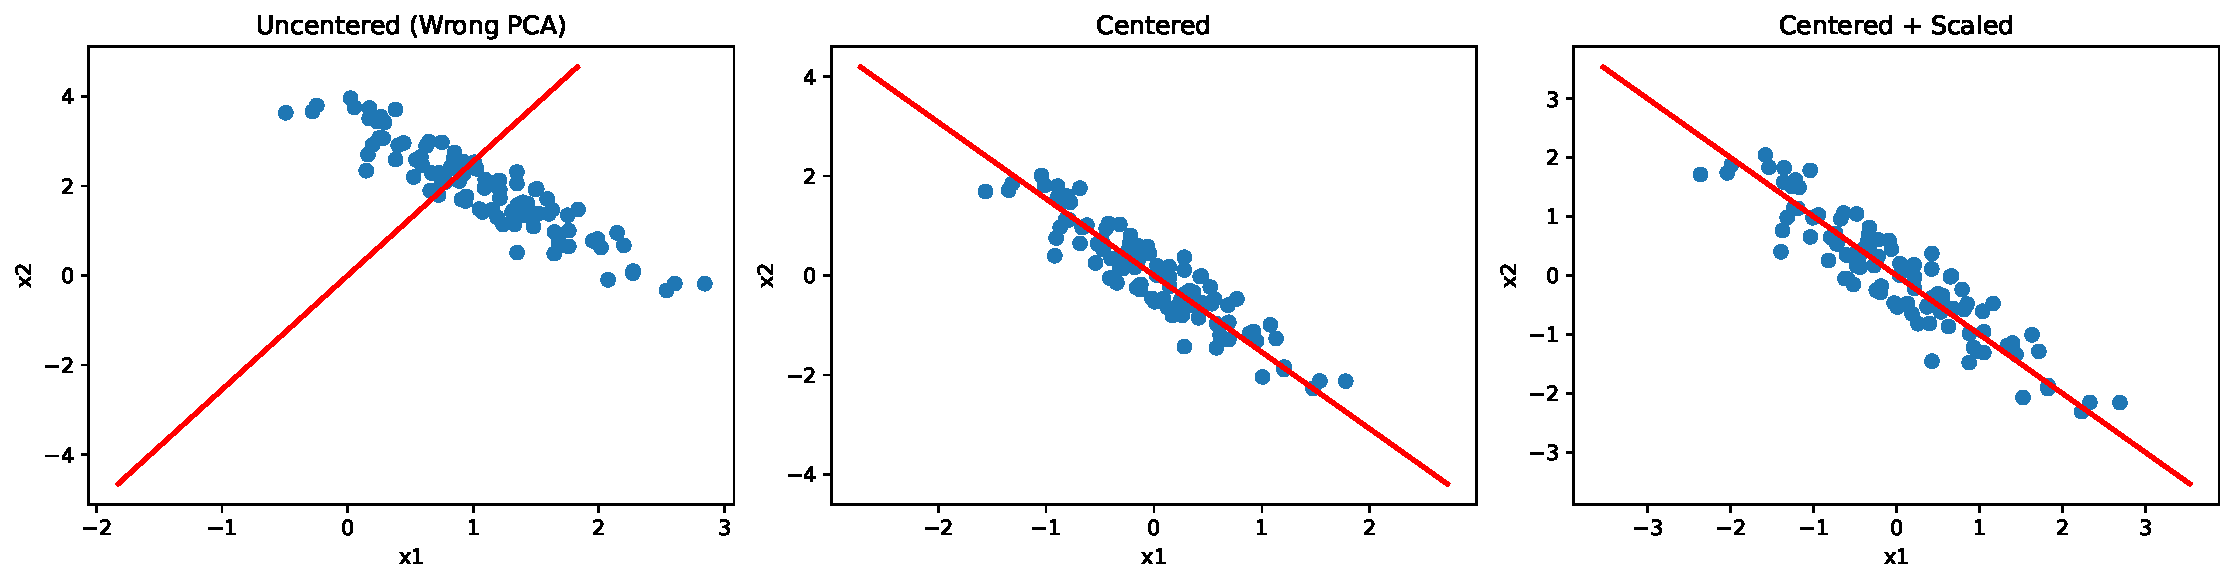
\includegraphics[keepaspectratio]{contents/1/dr_files/figure-pdf/cell-4-output-1.pdf}}

The principal component finds the direction that maximizes the variance
of the projected data.

If the data are not centered, the optimization is no longer based purely
on variance. In this case, the objective involves both the covariance
structure and the mean of the data.

As a result, when the mean is large, the first principal direction may
be strongly influenced by the location of the data, and can point
roughly toward the data cloud rather than reflecting its intrinsic
variation.

\end{example}

\begin{center}\rule{0.5\linewidth}{0.5pt}\end{center}

\subsection{Covariance and Optimality}\label{covariance-and-optimality}

The sample covariance matrix is \(S = \frac{1}{n-1} X^\top X\). By SVD,
\[
S=\frac{1}{n-1} X^\top X = V \frac{D^2}{n-1} V^\top
\]

\begin{itemize}
\tightlist
\item
  \(V\): eigenvectors of covariance matrix\\
\item
  \(d_j^2/(n-1)\): eigenvalues of \(S\)
\item
  \(\Var(Z_j)=d_j^2/(n-1)\)
\end{itemize}

Therefore

\begin{itemize}
\tightlist
\item
  First PC: Direction \(v_1\) that maximizes \(\Var(Xv_1)\) subject to
  \(\norm{v_1}=1\).
\item
  Subsequent PCs: Maximize remaining variance subject to orthogonality
  (that they are orthogonal to all previous PCs \(v_k^\top v_j = 0\) for
  \(j < k\)).
\end{itemize}

\begin{center}\rule{0.5\linewidth}{0.5pt}\end{center}

\subsection{Summary}\label{summary-1}

{\def\LTcaptype{none} % do not increment counter
\begin{longtable}[]{@{}
  >{\raggedright\arraybackslash}p{(\linewidth - 6\tabcolsep) * \real{0.2439}}
  >{\raggedright\arraybackslash}p{(\linewidth - 6\tabcolsep) * \real{0.1951}}
  >{\raggedright\arraybackslash}p{(\linewidth - 6\tabcolsep) * \real{0.1707}}
  >{\raggedright\arraybackslash}p{(\linewidth - 6\tabcolsep) * \real{0.3902}}@{}}
\toprule\noalign{}
\begin{minipage}[b]{\linewidth}\raggedright
Component
\end{minipage} & \begin{minipage}[b]{\linewidth}\raggedright
Matrix
\end{minipage} & \begin{minipage}[b]{\linewidth}\raggedright
Space
\end{minipage} & \begin{minipage}[b]{\linewidth}\raggedright
Interpretation
\end{minipage} \\
\midrule\noalign{}
\endhead
\bottomrule\noalign{}
\endlastfoot
Loadings & \(V\) & Feature (\(\mathbb{R}^p\)) & Principal directions
(rotation of axes) \\
Scores & \(Z = UD\) & Observation (\(\mathbb{R}^n\)) & Transformed
coordinates of observations \\
Normalized scores & \(U\) & Observation (\(\mathbb{R}^n\)) & Directions
of score vectors (unit length) \\
Singular values & \(D\) & --- & Scaling of each component (spread) \\
Variance & \(D^2/(n-1)\) & --- & Importance of each principal
component \\
\end{longtable}
}

\begin{itemize}
\tightlist
\item
  Columns of \(X\): variables in \(\mathbb{R}^n\) (relationships via
  angles)
\item
  Rows of \(X\): observations in \(\mathbb{R}^p\) (relationships via
  distance)
\item
  PCA finds orthogonal directions in feature space
\item
  \(V\) gives directions, \(Z\) gives coordinates
\item
  SVD unifies everything: \[
  X = UDV^\top, \quad Z = XV = UD
  \]
\end{itemize}

\begin{center}\rule{0.5\linewidth}{0.5pt}\end{center}

\subsection{\texorpdfstring{Choosing the number of components
(\(m\))}{Choosing the number of components (m)}}\label{choosing-the-number-of-components-m}

Let \(\rank(X)=r\). PCA produces \(r\) components, but in practice we
keep only the first \(m \le r\).

Define the truncated SVD: \[
X \approx X_m = U_m D_m V_m^\top,
\] where

\begin{itemize}
\tightlist
\item
  \(U_m \in \mathbb{R}^{n \times m}\)
\item
  \(D_m \in \mathbb{R}^{m \times m}\)
\item
  \(V_m \in \mathbb{R}^{p \times m}\)
\end{itemize}

Correspondingly, \[
Z_m = X V_m = U_m D_m
\] contains the first \(m\) principal components.

Keeping the \(m\) largest singular values gives the best rank-\(m\)
approximation of \(X\) in least squares sense.

\subsubsection{Variance explained}\label{variance-explained}

The total variance is \[
\sum_{j=1}^r \frac{d_j^2}{n-1},
\] and the proportion explained by the first \(m\) components is \[
\frac{\sum_{j=1}^m d_j^2}{\sum_{j=1}^r d_j^2}.
\]

\subsubsection{\texorpdfstring{Choosing \(m\) for prediction
(PCR)}{Choosing m for prediction (PCR)}}\label{choosing-m-for-prediction-pcr}

In predictive settings, \(m\) is typically selected via
cross-validation:

\begin{enumerate}
\def\labelenumi{\arabic{enumi}.}
\tightlist
\item
  Compute principal components.
\item
  Fit regression models using \(m = 1,2,\ldots,r\) components.
\item
  Evaluate validation error.
\item
  Choose \(m\) with the lowest validation error.
\end{enumerate}

\begin{tcolorbox}[enhanced jigsaw, arc=.35mm, bottomrule=.15mm, bottomtitle=1mm, breakable, colback=white, colbacktitle=quarto-callout-note-color!10!white, colframe=quarto-callout-note-color-frame, coltitle=black, left=2mm, leftrule=.75mm, opacityback=0, opacitybacktitle=0.6, rightrule=.15mm, title=\textcolor{quarto-callout-note-color}{\faInfo}\hspace{0.5em}{Scree plot (Elbow method)}, titlerule=0mm, toprule=.15mm, toptitle=1mm]

The scree plot (elbow method) plots \(d_j^2\) against \(j\) and selects
\(m\) at the point where the marginal gain in variance explained drops
sharply (the ``elbow''). This identifies the number of components that
captures most of the variation in \(X\).

However, PCA is unsupervised: directions that explain high variance in
\(X\) do not necessarily have strong predictive power for \(y\).
Therefore, in predictive settings such as PCR, \(m\) is typically chosen
via cross-validation rather than the elbow method.

For unsupervised tasks (e.g., representation or clustering), the scree
plot remains a reasonable and commonly used choice.

\end{tcolorbox}

\section{PCR in Python}\label{pcr-in-python}

\subsection{PCA}\label{pca}

\texttt{scikit-learn} provides \texttt{PCA} for computing principal
components. To demonstrate the code we use the same dataset from lasso.

\begin{Shaded}
\begin{Highlighting}[]
\ImportTok{import}\NormalTok{ numpy }\ImportTok{as}\NormalTok{ np}
\ImportTok{from}\NormalTok{ sklearn.model\_selection }\ImportTok{import}\NormalTok{ train\_test\_split}

\NormalTok{rng }\OperatorTok{=}\NormalTok{ np.random.default\_rng(}\DecValTok{0}\NormalTok{)}

\NormalTok{n }\OperatorTok{=} \DecValTok{150}
\NormalTok{p }\OperatorTok{=} \DecValTok{100}
\NormalTok{k }\OperatorTok{=} \DecValTok{12}

\NormalTok{Z }\OperatorTok{=}\NormalTok{ rng.normal(size}\OperatorTok{=}\NormalTok{(n, k))}
\NormalTok{A }\OperatorTok{=}\NormalTok{ rng.normal(size}\OperatorTok{=}\NormalTok{(k, p))}
\NormalTok{X }\OperatorTok{=}\NormalTok{ Z }\OperatorTok{@}\NormalTok{ A }\OperatorTok{+} \FloatTok{0.8} \OperatorTok{*}\NormalTok{ rng.normal(size}\OperatorTok{=}\NormalTok{(n, p))}

\NormalTok{beta }\OperatorTok{=}\NormalTok{ np.zeros(p)}
\NormalTok{beta[:}\DecValTok{10}\NormalTok{] }\OperatorTok{=}\NormalTok{ [}\DecValTok{8}\NormalTok{, }\DecValTok{7}\NormalTok{, }\DecValTok{6}\NormalTok{, }\DecValTok{5}\NormalTok{, }\DecValTok{4}\NormalTok{, }\DecValTok{3}\NormalTok{, }\DecValTok{2}\NormalTok{, }\FloatTok{1.5}\NormalTok{, }\DecValTok{1}\NormalTok{, }\FloatTok{0.5}\NormalTok{]}

\NormalTok{y }\OperatorTok{=}\NormalTok{ X }\OperatorTok{@}\NormalTok{ beta }\OperatorTok{+} \DecValTok{12} \OperatorTok{*}\NormalTok{ rng.normal(size}\OperatorTok{=}\NormalTok{n)}

\NormalTok{X\_train, X\_test, y\_train, y\_test }\OperatorTok{=}\NormalTok{ train\_test\_split(}
\NormalTok{    X, y, test\_size}\OperatorTok{=}\FloatTok{0.3}\NormalTok{, random\_state}\OperatorTok{=}\DecValTok{0}
\NormalTok{)}
\end{Highlighting}
\end{Shaded}

\texttt{pca} is an unsupervised learnning method. Therefore to perform
it we only need \texttt{X}.

\begin{Shaded}
\begin{Highlighting}[]
\ImportTok{from}\NormalTok{ sklearn.decomposition }\ImportTok{import}\NormalTok{ PCA}

\NormalTok{pca }\OperatorTok{=}\NormalTok{ PCA().fit(X\_train)}
\end{Highlighting}
\end{Shaded}

All important information can be accessed from the returned object.

\begin{Shaded}
\begin{Highlighting}[]
\NormalTok{V }\OperatorTok{=}\NormalTok{ pca.components\_.T                   }\CommentTok{\# loadings (V)}
\NormalTok{Z }\OperatorTok{=}\NormalTok{ pca.transform(X\_train)              }\CommentTok{\# scores (Z)}
\NormalTok{D }\OperatorTok{=}\NormalTok{ pca.singular\_values\_                }\CommentTok{\# singular values (D)}
\NormalTok{var }\OperatorTok{=}\NormalTok{ pca.explained\_variance\_           }\CommentTok{\# variance that are explained}
\NormalTok{ratio }\OperatorTok{=}\NormalTok{ pca.explained\_variance\_ratio\_   }\CommentTok{\# the ratio of variance that are explained}
\end{Highlighting}
\end{Shaded}

With \texttt{var} and \texttt{ratio}, we may plot the scree plot
(although we won't really use it to select the number of components).

\protect\phantomsection\label{annotated-cell-97}%
\begin{Shaded}
\begin{Highlighting}[]
\NormalTok{k }\OperatorTok{=}\NormalTok{ np.arange(}\DecValTok{1}\NormalTok{, }\BuiltInTok{len}\NormalTok{(var) }\OperatorTok{+} \DecValTok{1}\NormalTok{)}

\NormalTok{plt.figure()}
\NormalTok{plt.plot(k, ratio, marker}\OperatorTok{=}\StringTok{"o"}\NormalTok{)}
\NormalTok{plt.xlabel(}\StringTok{"Component index"}\NormalTok{)}
\NormalTok{plt.ylabel(}\StringTok{"Proportion of variance explained"}\NormalTok{)}
\NormalTok{plt.title(}\StringTok{"Scree Plot (Variance Ratio)"}\NormalTok{)}

\NormalTok{cum }\OperatorTok{=}\NormalTok{ np.cumsum(ratio)}

\NormalTok{diff2 }\OperatorTok{=}\NormalTok{ np.diff(cum, }\DecValTok{2}\NormalTok{)}
\NormalTok{elbow\_idx }\OperatorTok{=}\NormalTok{ np.argmin(diff2) }\OperatorTok{+} \DecValTok{2}
\NormalTok{elbow\_k }\OperatorTok{=}\NormalTok{ k[elbow\_idx]}
\NormalTok{elbow\_val }\OperatorTok{=}\NormalTok{ ratio[elbow\_idx]}
\NormalTok{plt.axvline(elbow\_k, linestyle}\OperatorTok{=}\StringTok{"{-}{-}"}\NormalTok{, color}\OperatorTok{=}\StringTok{"red"}\NormalTok{) }\CommentTok{\# \textless{}1\textgreater{}}

\NormalTok{plt.scatter(elbow\_k, elbow\_val)}
\NormalTok{plt.text(elbow\_k }\OperatorTok{+} \FloatTok{0.2}\NormalTok{, elbow\_val }\OperatorTok{+} \FloatTok{0.004}\NormalTok{, }\SpecialStringTok{f"k=}\SpecialCharTok{\{}\NormalTok{elbow\_k}\SpecialCharTok{\}}\CharTok{\textbackslash{}n}\SpecialCharTok{\{}\NormalTok{elbow\_val}\SpecialCharTok{:.3f\}}\SpecialStringTok{"}\NormalTok{)}
\end{Highlighting}
\end{Shaded}

\begin{description}
\tightlist
\item[5CB6E08D-list-annote-1]
Use 2nd order difference to find the elbow.
\end{description}

\begin{verbatim}
Text(13.2, 0.005666697882320329, 'k=13\n0.002')
\end{verbatim}

\pandocbounded{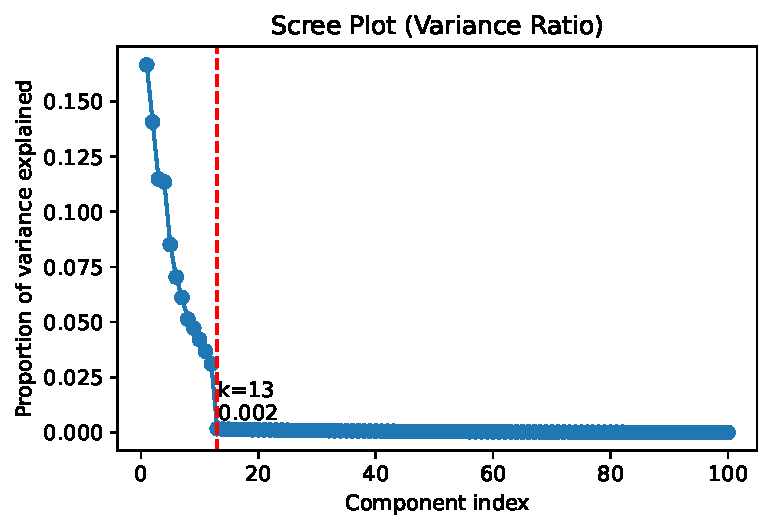
\includegraphics[keepaspectratio]{contents/1/dr_files/figure-pdf/cell-8-output-2.pdf}}

\subsection{PCR}\label{pcr}

Using PCA to do regression, we have to standarize the data. Therefore we
set up the pipeline.

We first use 13 components (which comes from the scree plot) as our
starting point. We will tune it later using cross-validation.

\begin{Shaded}
\begin{Highlighting}[]
\ImportTok{from}\NormalTok{ sklearn.pipeline }\ImportTok{import}\NormalTok{ Pipeline}
\ImportTok{from}\NormalTok{ sklearn.preprocessing }\ImportTok{import}\NormalTok{ StandardScaler}
\ImportTok{from}\NormalTok{ sklearn.linear\_model }\ImportTok{import}\NormalTok{ LinearRegression}
\ImportTok{from}\NormalTok{ sklearn.metrics }\ImportTok{import}\NormalTok{ mean\_squared\_error, r2\_score}

\NormalTok{pcr\_pipe }\OperatorTok{=}\NormalTok{ Pipeline(}
\NormalTok{    [}
\NormalTok{        (}\StringTok{"scaler"}\NormalTok{, StandardScaler()),}
\NormalTok{        (}\StringTok{"pca"}\NormalTok{, PCA(n\_components}\OperatorTok{=}\DecValTok{13}\NormalTok{)),}
\NormalTok{        (}\StringTok{"model"}\NormalTok{, LinearRegression()),}
\NormalTok{    ]}
\NormalTok{)}

\NormalTok{pcr\_pipe.fit(X\_train, y\_train)}
\NormalTok{y\_pred\_pcr }\OperatorTok{=}\NormalTok{ pcr\_pipe.predict(X\_test)}

\BuiltInTok{print}\NormalTok{(}\SpecialStringTok{f"Test RMSE: }\SpecialCharTok{\{}\NormalTok{mean\_squared\_error(y\_test, y\_pred\_pcr)}\SpecialCharTok{\}}\SpecialStringTok{"}\NormalTok{)}
\BuiltInTok{print}\NormalTok{(}\SpecialStringTok{f"Test R\^{}2 : }\SpecialCharTok{\{}\NormalTok{r2\_score(y\_test, y\_pred\_pcr)}\SpecialCharTok{\}}\SpecialStringTok{"}\NormalTok{)}
\end{Highlighting}
\end{Shaded}

\begin{verbatim}
Test RMSE: 348.7698605548008
Test R^2 : 0.8536528530700276
\end{verbatim}

You may compare it with the results we get from \texttt{lasso} and
\texttt{ridge}.

\subsection{Choosing number of components by
cross-validation}\label{choosing-number-of-components-by-cross-validation}

We use \(K\)-fold cross validation to find the best number of
components. Our criterion is negative MSE.

\protect\phantomsection\label{annotated-cell-99}%
\begin{Shaded}
\begin{Highlighting}[]
\ImportTok{from}\NormalTok{ sklearn.model\_selection }\ImportTok{import}\NormalTok{ GridSearchCV}

\NormalTok{n\_splits }\OperatorTok{=} \DecValTok{5}
\NormalTok{n\_train\_fold }\OperatorTok{=} \BuiltInTok{int}\NormalTok{(X\_train.shape[}\DecValTok{0}\NormalTok{] }\OperatorTok{*}\NormalTok{ (n\_splits }\OperatorTok{{-}} \DecValTok{1}\NormalTok{) }\OperatorTok{/}\NormalTok{ n\_splits)}
\NormalTok{max\_components }\OperatorTok{=} \BuiltInTok{min}\NormalTok{(n\_train\_fold, X\_train.shape[}\DecValTok{1}\NormalTok{]) }\CommentTok{\# \textless{}1\textgreater{}}

\NormalTok{param\_grid }\OperatorTok{=}\NormalTok{ \{}\StringTok{"pca\_\_n\_components"}\NormalTok{: }\BuiltInTok{list}\NormalTok{(}\BuiltInTok{range}\NormalTok{(}\DecValTok{1}\NormalTok{, max\_components }\OperatorTok{+} \DecValTok{1}\NormalTok{))\}}

\NormalTok{gs\_pcr }\OperatorTok{=}\NormalTok{ GridSearchCV(}
\NormalTok{    pcr\_pipe, param\_grid, cv}\OperatorTok{=}\NormalTok{n\_splits, scoring}\OperatorTok{=}\StringTok{"neg\_mean\_squared\_error"}
\NormalTok{)}
\NormalTok{gs\_pcr.fit(X\_train, y\_train)}
\NormalTok{gs\_pcr.best\_params\_[}\StringTok{"pca\_\_n\_components"}\NormalTok{]}
\end{Highlighting}
\end{Shaded}

\begin{description}
\tightlist
\item[5CB6E08D-list-annote-1]
The maximal possible number of components depends on the shape of X.
However for cross-validation, the number of rows of X is reduced due to
the split. Therefore we have to estimate this number in order to avoid
``\texttt{n\_components} out of bounds'' warning.
\end{description}

\begin{verbatim}
19
\end{verbatim}

It shows that 19 is the best number. Then we check the test result.

\begin{Shaded}
\begin{Highlighting}[]
\NormalTok{y\_pred\_pcr }\OperatorTok{=}\NormalTok{ gs\_pcr.predict(X\_test)}

\BuiltInTok{print}\NormalTok{(}\SpecialStringTok{f"Test RMSE: }\SpecialCharTok{\{}\NormalTok{mean\_squared\_error(y\_test, y\_pred\_pcr)}\SpecialCharTok{\}}\SpecialStringTok{"}\NormalTok{)}
\BuiltInTok{print}\NormalTok{(}\SpecialStringTok{f"Test R\^{}2 : }\SpecialCharTok{\{}\NormalTok{r2\_score(y\_test, y\_pred\_pcr)}\SpecialCharTok{\}}\SpecialStringTok{"}\NormalTok{)}
\end{Highlighting}
\end{Shaded}

\begin{verbatim}
Test RMSE: 321.0762521471908
Test R^2 : 0.8652733542572647
\end{verbatim}

It is slightly better than \texttt{13}, but still worse than tuned
\texttt{ridge} and \texttt{lasso}.

We could also look at the validation curve on the mean test score.

\begin{Shaded}
\begin{Highlighting}[]
\ImportTok{import}\NormalTok{ matplotlib.pyplot }\ImportTok{as}\NormalTok{ plt}

\NormalTok{plt.plot(param\_grid[}\StringTok{"pca\_\_n\_components"}\NormalTok{], gs\_pcr.cv\_results\_[}\StringTok{"mean\_test\_score"}\NormalTok{])}
\NormalTok{plt.axvline(}\DecValTok{19}\NormalTok{, linestyle}\OperatorTok{=}\StringTok{"{-}{-}"}\NormalTok{, color}\OperatorTok{=}\StringTok{"red"}\NormalTok{, label}\OperatorTok{=}\StringTok{"best\_gs"}\NormalTok{)}
\NormalTok{plt.axvline(}\DecValTok{13}\NormalTok{, linestyle}\OperatorTok{=}\StringTok{"{-}{-}"}\NormalTok{, color}\OperatorTok{=}\StringTok{"blue"}\NormalTok{, label}\OperatorTok{=}\StringTok{"best\_elbow"}\NormalTok{)}
\NormalTok{plt.legend()}
\end{Highlighting}
\end{Shaded}

\pandocbounded{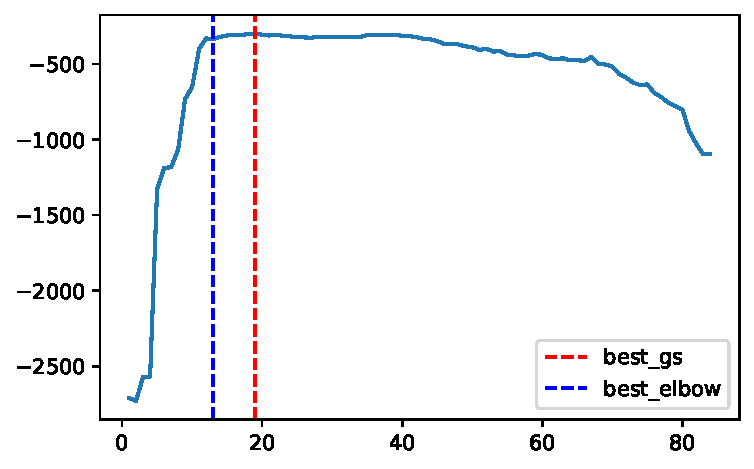
\includegraphics[keepaspectratio]{contents/1/dr_files/figure-pdf/cell-12-output-1.pdf}}

\section{Partial Least Squares (PLS)}\label{partial-least-squares-pls}

One limitation of Principal Component Regression (PCR) is that it is
unsupervised: the principal components depend only on \(X\) and ignore
the response \(y\). As a result, directions with large variance in \(X\)
may not be relevant for predicting \(y\).

Partial Least Squares (PLS) addresses this by constructing components
that are guided by the response. It seeks directions in the predictor
space that are both:

\begin{itemize}
\tightlist
\item
  informative about \(X\), and
\item
  strongly related to \(y\)
\end{itemize}

\begin{definition}[Partial Least
Squares]\protect\hypertarget{def-pls}{}\label{def-pls}

Partial least squares constructs a sequence of components

\[
Z_k = X w_k
\]

where the weight vector \(w_k\) is chosen to maximize the covariance
between the component and the response: \[
w_k =\arg\max_{\norm{w}=1}\Cov(Xw, y).
\]

After constructing the component \(Z_k\), both the predictor matrix
\(X\) and the response \(y\) are deflated, and the procedure is repeated
to construct additional components.

\end{definition}

\subsection{Algorithm intuition}\label{algorithm-intuition}

PLS constructs components sequentially, with each step explicitly
targeting predictive power for \(y\), rather than variance in \(X\).

\textbf{Step 1}: Find the direction. Choose a direction
\(w_k \in \mathbb{R}^p\) such that the component \(Z_k = X_k w_k\)
maximizes covariance with \(y_k\). \[
w_k =\arg\max_{\norm{w}=1}\Cov(X_kw, y_k)
\]

\textbf{Step 2}: Define the \(k\)-th component (also called the score
vector): \[
Z_k=X_kw_k\in\mathbb R^n
\]

\begin{itemize}
\tightlist
\item
  This is a linear combination of predictors
\item
  Represents the direction in \(X\) most aligned with \(y_k\)
\end{itemize}

\textbf{Step 3}: Fit a simple regression of \(y_k\) on \(Z_k\): \[
y_k=c_kZ_k+\resid
\] This captures how strongly the component explains \(y_k\).

\textbf{Step 4}: Deflation: remove the variation explained by \(Z_k\)
from both \(X_k\) and \(y_k\).

\begin{itemize}
\tightlist
\item
  Update response: \(y_{k+1}=y_k-c_kZ_k\)
\item
  Update predictors: \(X_{k+1}=X_k-Z_kp_k^\top\), where
  \(p_k=\frac{X_k^\top Z_k}{Z_k^\top Z_k}\).

  \begin{itemize}
  \tightlist
  \item
    \(p_k\) are the loadings for reconstructing \(X\)
  \item
    Deflation ensures the next components capture on new information
  \end{itemize}
\end{itemize}

\textbf{Step 5}: Repeat the process for \(k = 1, 2, \dots, m\).

\subsection{Key properties}\label{key-properties}

PLS has several important structural properties:

\begin{itemize}
\tightlist
\item
  The components \(\{Z_1, Z_2, \dots\}\) are constructed sequentially.\\
\item
  Each component explains the remaining variation in \(y\).\\
\item
  After deflation, the components are orthogonal.\\
\item
  The ordering reflects predictive importance.
\end{itemize}

At each step, the main quantities have distinct roles:

{\def\LTcaptype{none} % do not increment counter
\begin{longtable}[]{@{}ll@{}}
\toprule\noalign{}
Quantity & Interpretation \\
\midrule\noalign{}
\endhead
\bottomrule\noalign{}
\endlastfoot
\(w_k\) & Direction in feature space used to combine predictors \\
\(Z_k = X_k w_k\) & Score (component), representing projected data \\
\(p_k\) & Loading, describing how the component explains \(X\) \\
\end{longtable}
}

Together, these quantities describe how information is extracted from
\(X\) and transferred to explain \(y\).

\subsection{Comparison with PCA}\label{comparison-with-pca}

The key difference between PCA and PLS lies in how the directions are
chosen:

{\def\LTcaptype{none} % do not increment counter
\begin{longtable}[]{@{}
  >{\raggedright\arraybackslash}p{(\linewidth - 4\tabcolsep) * \real{0.0896}}
  >{\raggedright\arraybackslash}p{(\linewidth - 4\tabcolsep) * \real{0.5373}}
  >{\raggedright\arraybackslash}p{(\linewidth - 4\tabcolsep) * \real{0.3731}}@{}}
\toprule\noalign{}
\begin{minipage}[b]{\linewidth}\raggedright
Method
\end{minipage} & \begin{minipage}[b]{\linewidth}\raggedright
Criterion
\end{minipage} & \begin{minipage}[b]{\linewidth}\raggedright
Interpretation
\end{minipage} \\
\midrule\noalign{}
\endhead
\bottomrule\noalign{}
\endlastfoot
PCA & maximize \(\operatorname{Var}(Xw)\) & captures structure of
\(X\) \\
PLS & maximize \(\operatorname{Cov}(Xw, y)\) & targets prediction of
\(y\) \\
\end{longtable}
}

PCA captures the internal structure of \(X\), while PLS focuses on
directions that are useful for predicting \(y\).

\subsection{Geometric meaning (Krylov
Subspace)}\label{geometric-meaning-krylov-subspace}

The matrix \(X\) defines a cloud of points in \(\mathbb{R}^p\) and the
response \(y\) defines a direction in \(\mathbb{R}^n\).

PLS finds directions \(w_k\) such that the projections \(Z_k = X w_k\)
are maximally aligned with \(y\) in the observation space. In this
sense, PLS can be understood geometrically as searching for directions
in predictor space that align with the response.

To be more precise, it can be explained using Krylov subspaces.

Click to expand.

The Krylov subspace provides a structured way to generate directions for
solving regression problems. Instead of searching the entire feature
space \(\mathbb{R}^p\), it builds a sequence of low-dimensional
subspaces that are tailored to the problem.

Given a matrix \(A \in \mathbb{R}^{p \times p}\) and a vector
\(b \in \mathbb{R}^p\), the Krylov subspace of order \(k\) is defined as
\[
\mathcal{K}_k(A, b)
=
\operatorname{span}\{b,\; Ab,\; A^2 b,\; \dots,\; A^{k-1} b\}.
\]

The subspaces are nested, meaning
\(\mathcal{K}_1 \subseteq \mathcal{K}_2 \subseteq \cdots\), and the
dimension cannot exceed \(\rank(A)\). Therefore, the sequence stabilizes
after at most \(\rank(A)\) steps.

\subsubsection{Krylov Subspace in
Regression}\label{krylov-subspace-in-regression}

In linear regression, we take \[
A = X^\top X, \qquad b = X^\top y.
\]

Then the Krylov subspace becomes \[
\mathcal{K}_k(X^\top X, X^\top y)
=
\operatorname{span}\{X^\top y,\ (X^\top X)X^\top y,\ (X^\top X)^2 X^\top y,\dots\}.
\]

The vector \(X^\top y\) represents directions in the predictor space
that are most correlated with the response, while \(X^\top X\) encodes
the covariance structure of the predictors. As a result, the Krylov
subspace captures directions that are both aligned with \(y\) and
consistent with the geometry of \(X\).

\subsubsection{Connection to PLS}\label{connection-to-pls}

Partial Least Squares constructs its directions sequentially within the
Krylov subspace: \[
w_k \in \mathcal{K}_k(X^\top X,\; X^\top y).
\]

This means that PLS does not search over all possible directions in
\(\mathbb{R}^p\). Instead, it expands a problem-dependent subspace step
by step, starting from \(X^\top y\) and incorporating higher-order
interactions through \(X^\top X\).

The number of components is therefore bounded by \[
m \le \dim(\mathcal{K}_k) \le \rank(X).
\]

\begin{tcolorbox}[enhanced jigsaw, arc=.35mm, bottomrule=.15mm, bottomtitle=1mm, breakable, colback=white, colbacktitle=quarto-callout-note-color!10!white, colframe=quarto-callout-note-color-frame, coltitle=black, left=2mm, leftrule=.75mm, opacityback=0, opacitybacktitle=0.6, rightrule=.15mm, title=\textcolor{quarto-callout-note-color}{\faInfo}\hspace{0.5em}{Note}, titlerule=0mm, toprule=.15mm, toptitle=1mm]

The Krylov subspace can be viewed as a guided search path inside
\(\operatorname{span}(X)\). The first direction is determined by
\(X^\top y\), and subsequent directions refine this information by
incorporating the covariance structure of the predictors.

In this sense, the Krylov subspace represents the portion of the feature
space that is relevant for predicting \(y\). Methods such as PLS operate
within this space, focusing on directions that carry predictive signal
rather than exploring the entire feature space.

\end{tcolorbox}

\section{PLS in Python}\label{pls-in-python}

Although the algorithm is different, the code is very similar to PCR.
PLS is implemented by \texttt{PLSRegression} from
\texttt{sklearn.cross\_decomposition}. The argument \texttt{scale=True}
is by default so we don't need to attach standardizer to it.

We choose the default number of componenets (which is 2) here. The
specific hyperparameter will be tuned later by cross-validation.

\begin{Shaded}
\begin{Highlighting}[]
\ImportTok{from}\NormalTok{ sklearn.cross\_decomposition }\ImportTok{import}\NormalTok{ PLSRegression}

\NormalTok{pls }\OperatorTok{=}\NormalTok{ PLSRegression()}

\NormalTok{pls.fit(X\_train, y\_train)}
\end{Highlighting}
\end{Shaded}

We could use the following code to get access to the parameters.

\begin{Shaded}
\begin{Highlighting}[]
\NormalTok{W }\OperatorTok{=}\NormalTok{ pls.x\_weights\_    }\CommentTok{\# weights, directions (W)}
\NormalTok{Z }\OperatorTok{=}\NormalTok{ pls.x\_scores\_     }\CommentTok{\# scores, components (Z)}
\NormalTok{P }\OperatorTok{=}\NormalTok{ pls.x\_loadings\_   }\CommentTok{\# loadings (P)}
\end{Highlighting}
\end{Shaded}

\subsection{Example}\label{example}

We use the same simulated dataset as before.

\begin{Shaded}
\begin{Highlighting}[]
\ImportTok{import}\NormalTok{ numpy }\ImportTok{as}\NormalTok{ np}
\ImportTok{from}\NormalTok{ sklearn.model\_selection }\ImportTok{import}\NormalTok{ train\_test\_split}

\NormalTok{rng }\OperatorTok{=}\NormalTok{ np.random.default\_rng(}\DecValTok{0}\NormalTok{)}

\NormalTok{n }\OperatorTok{=} \DecValTok{150}
\NormalTok{p }\OperatorTok{=} \DecValTok{100}
\NormalTok{k }\OperatorTok{=} \DecValTok{12}

\NormalTok{Z }\OperatorTok{=}\NormalTok{ rng.normal(size}\OperatorTok{=}\NormalTok{(n, k))}
\NormalTok{A }\OperatorTok{=}\NormalTok{ rng.normal(size}\OperatorTok{=}\NormalTok{(k, p))}
\NormalTok{X }\OperatorTok{=}\NormalTok{ Z }\OperatorTok{@}\NormalTok{ A }\OperatorTok{+} \FloatTok{0.8} \OperatorTok{*}\NormalTok{ rng.normal(size}\OperatorTok{=}\NormalTok{(n, p))}

\NormalTok{beta }\OperatorTok{=}\NormalTok{ np.zeros(p)}
\NormalTok{beta[:}\DecValTok{10}\NormalTok{] }\OperatorTok{=}\NormalTok{ [}\DecValTok{8}\NormalTok{, }\DecValTok{7}\NormalTok{, }\DecValTok{6}\NormalTok{, }\DecValTok{5}\NormalTok{, }\DecValTok{4}\NormalTok{, }\DecValTok{3}\NormalTok{, }\DecValTok{2}\NormalTok{, }\FloatTok{1.5}\NormalTok{, }\DecValTok{1}\NormalTok{, }\FloatTok{0.5}\NormalTok{]}

\NormalTok{y }\OperatorTok{=}\NormalTok{ X }\OperatorTok{@}\NormalTok{ beta }\OperatorTok{+} \DecValTok{12} \OperatorTok{*}\NormalTok{ rng.normal(size}\OperatorTok{=}\NormalTok{n)}

\NormalTok{X\_train, X\_test, y\_train, y\_test }\OperatorTok{=}\NormalTok{ train\_test\_split(}
\NormalTok{    X, y, test\_size}\OperatorTok{=}\FloatTok{0.3}\NormalTok{, random\_state}\OperatorTok{=}\DecValTok{0}
\NormalTok{)}
\end{Highlighting}
\end{Shaded}

Similar to PCR, we need to choose the number of components. Since PLS is
fit inside cross-validation, the maximum number of components should be
no larger than the number of observations in each training fold.

\begin{Shaded}
\begin{Highlighting}[]
\ImportTok{from}\NormalTok{ sklearn.model\_selection }\ImportTok{import}\NormalTok{ GridSearchCV}
\ImportTok{from}\NormalTok{ sklearn.cross\_decomposition }\ImportTok{import}\NormalTok{ PLSRegression}

\NormalTok{n\_splits }\OperatorTok{=} \DecValTok{5}
\NormalTok{n\_train\_fold }\OperatorTok{=} \BuiltInTok{int}\NormalTok{(X\_train.shape[}\DecValTok{0}\NormalTok{] }\OperatorTok{*}\NormalTok{ (n\_splits }\OperatorTok{{-}} \DecValTok{1}\NormalTok{) }\OperatorTok{/}\NormalTok{ n\_splits)}
\NormalTok{max\_components }\OperatorTok{=} \BuiltInTok{min}\NormalTok{(n\_train\_fold, X\_train.shape[}\DecValTok{1}\NormalTok{])}

\NormalTok{param\_grid }\OperatorTok{=}\NormalTok{ \{}\StringTok{"n\_components"}\NormalTok{: }\BuiltInTok{list}\NormalTok{(}\BuiltInTok{range}\NormalTok{(}\DecValTok{1}\NormalTok{, max\_components }\OperatorTok{+} \DecValTok{1}\NormalTok{))\}}

\NormalTok{gs\_pls }\OperatorTok{=}\NormalTok{ GridSearchCV(}
\NormalTok{    PLSRegression(), param\_grid, cv}\OperatorTok{=}\NormalTok{n\_splits, scoring}\OperatorTok{=}\StringTok{"neg\_mean\_squared\_error"}
\NormalTok{)}
\NormalTok{gs\_pls.fit(X\_train, y\_train)}
\NormalTok{gs\_pls.best\_params\_[}\StringTok{"n\_components"}\NormalTok{]}
\end{Highlighting}
\end{Shaded}

\begin{verbatim}
4
\end{verbatim}

After selecting the number of components by cross-validation, we
evaluate the fitted model on the test set.

\begin{Shaded}
\begin{Highlighting}[]
\NormalTok{y\_pred\_pls }\OperatorTok{=}\NormalTok{ gs\_pls.predict(X\_test)}

\BuiltInTok{print}\NormalTok{(}\SpecialStringTok{f"Test RMSE: }\SpecialCharTok{\{}\NormalTok{mean\_squared\_error(y\_test, y\_pred\_pls)}\SpecialCharTok{\}}\SpecialStringTok{"}\NormalTok{)}
\BuiltInTok{print}\NormalTok{(}\SpecialStringTok{f"Test R\^{}2 : }\SpecialCharTok{\{}\NormalTok{r2\_score(y\_test, y\_pred\_pls)}\SpecialCharTok{\}}\SpecialStringTok{"}\NormalTok{)}
\end{Highlighting}
\end{Shaded}

\begin{verbatim}
Test RMSE: 333.9484272722302
Test R^2 : 0.8598720672844287
\end{verbatim}

The validation curve shows how the cross-validation error changes as the
number of PLS components increases.

\begin{Shaded}
\begin{Highlighting}[]
\ImportTok{import}\NormalTok{ matplotlib.pyplot }\ImportTok{as}\NormalTok{ plt}

\NormalTok{plt.plot(param\_grid[}\StringTok{"n\_components"}\NormalTok{], gs\_pls.cv\_results\_[}\StringTok{"mean\_test\_score"}\NormalTok{])}
\NormalTok{plt.axvline(}
\NormalTok{    gs\_pls.best\_params\_[}\StringTok{"n\_components"}\NormalTok{],}
\NormalTok{    linestyle}\OperatorTok{=}\StringTok{"{-}{-}"}\NormalTok{,}
\NormalTok{    color}\OperatorTok{=}\StringTok{"red"}\NormalTok{,}
\NormalTok{    label}\OperatorTok{=}\StringTok{"best\_gs"}\NormalTok{,}
\NormalTok{)}
\NormalTok{plt.legend()}
\end{Highlighting}
\end{Shaded}

\pandocbounded{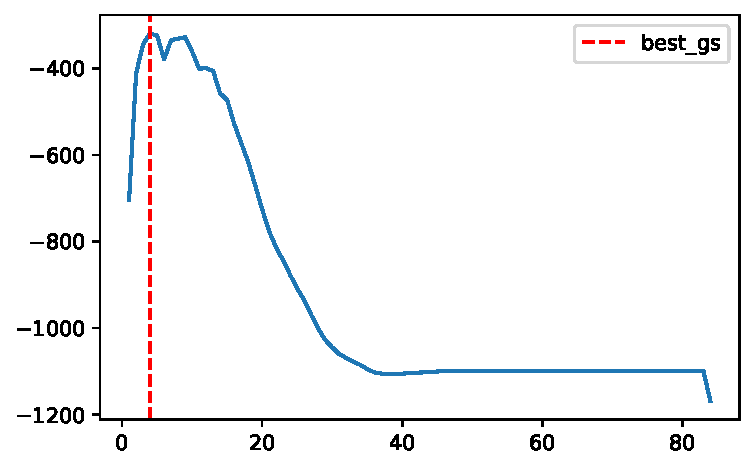
\includegraphics[keepaspectratio]{contents/1/dr_files/figure-pdf/cell-18-output-1.pdf}}

\begin{tcolorbox}[enhanced jigsaw, arc=.35mm, bottomrule=.15mm, bottomtitle=1mm, breakable, colback=white, colbacktitle=quarto-callout-note-color!10!white, colframe=quarto-callout-note-color-frame, coltitle=black, left=2mm, leftrule=.75mm, opacityback=0, opacitybacktitle=0.6, rightrule=.15mm, title=\textcolor{quarto-callout-note-color}{\faInfo}\hspace{0.5em}{Important Notes}, titlerule=0mm, toprule=.15mm, toptitle=1mm]

\begin{itemize}
\tightlist
\item
  \texttt{PLSRegression} automatically centers and scales the predictors
  by default.
\item
  Unlike PCR, PLS uses both \(X\) and \(y\) when constructing
  components.
\item
  The number of components should be chosen by cross-validation.
\item
  Very large numbers of components are usually unnecessary and may lead
  to numerical warnings.
\end{itemize}

\end{tcolorbox}

The results for this dataset are summarized in the following table.

{\def\LTcaptype{none} % do not increment counter
\begin{longtable}[]{@{}llll@{}}
\toprule\noalign{}
& Test RMSE & Test R² & Best param \\
Model & & & \\
\midrule\noalign{}
\endhead
\bottomrule\noalign{}
\endlastfoot
OLS & 1212.5155 & 0.491217 & NaN \\
RidgeCV & 274.2522 & 0.884921 & alpha=10.0 \\
LassoCV & 221.7648 & 0.906945 & alpha=0.4608014833934263 \\
PCR & 321.0763 & 0.865273 & n\_components=19 \\
PLS & 333.9484 & 0.859872 & n\_components=4 \\
\end{longtable}
}

Note that PCR and PLS do not perform as well as ridge and lasso in this
example. A key reason lies in how the dataset is generated.

\begin{itemize}
\tightlist
\item
  The coefficient vector \(\beta\) is sparse: only a small number of
  predictors (10 out of 100) are truly relevant.
\item
  The noise level is relatively high, making signal recovery more
  difficult.
\item
  More importantly, the variation in \(X\) is driven by a
  low-dimensional latent structure (\(Z A\)), while the true signal
  depends on a sparse set of original predictors. As a result, the
  directions of largest variance in \(X\) are not necessarily aligned
  with the directions that predict \(y\).
\end{itemize}

Since PCR relies only on variance in \(X\), and PLS is still influenced
by this structure, both methods may fail to recover the true signal
efficiently. In contrast, ridge and lasso operate directly on the
original predictors, with lasso particularly well-suited for identifying
sparse signals.

\subsection{Another example}\label{another-example}

Now let us look at another example. In this setting, we construct \(X\)
so that most of its variance comes from irrelevant noise, while the true
signal has low variance but determines \(y\). Specifically, \[
y = Z_1 b + \varepsilon_Y, \quad
X = Z_1 A_1 + Z_2 A_2 + \varepsilon_X.
\]

This setup has the following properties:

\begin{itemize}
\tightlist
\item
  \(Z_1\) (signal) has low variance, while \(Z_2\) (noise) has high
  variance.
\item
  \(y\) depends only on \(Z_1\).
\item
  Therefore, the predictive signal lies in low-variance but structured
  (low-rank) directions of \(X\).
\item
  For simplicity, we take \(Z_1\) to be one-dimensional in the following
  example.
\end{itemize}

\begin{Shaded}
\begin{Highlighting}[]
\ImportTok{import}\NormalTok{ numpy }\ImportTok{as}\NormalTok{ np}

\NormalTok{rng }\OperatorTok{=}\NormalTok{ np.random.default\_rng(}\DecValTok{42}\NormalTok{)}

\NormalTok{n }\OperatorTok{=} \DecValTok{120}
\NormalTok{p }\OperatorTok{=} \DecValTok{300}

\NormalTok{Z\_1 }\OperatorTok{=}\NormalTok{ rng.normal(size}\OperatorTok{=}\NormalTok{(n, }\DecValTok{1}\NormalTok{))}
\NormalTok{A\_1 }\OperatorTok{=}\NormalTok{ rng.normal(size}\OperatorTok{=}\NormalTok{(}\DecValTok{1}\NormalTok{, p))}
\NormalTok{X\_signal }\OperatorTok{=}\NormalTok{ Z\_1 }\OperatorTok{@}\NormalTok{ A\_1 }\OperatorTok{*} \FloatTok{0.15}

\NormalTok{k\_2 }\OperatorTok{=} \DecValTok{10}
\NormalTok{Z\_2 }\OperatorTok{=}\NormalTok{ rng.normal(size}\OperatorTok{=}\NormalTok{(n, k\_2))}
\NormalTok{A\_2 }\OperatorTok{=}\NormalTok{ rng.normal(size}\OperatorTok{=}\NormalTok{(k\_2, p))}
\NormalTok{X\_noise }\OperatorTok{=}\NormalTok{ Z\_2 }\OperatorTok{@}\NormalTok{ A\_2 }\OperatorTok{*} \DecValTok{15}

\NormalTok{X }\OperatorTok{=}\NormalTok{ X\_noise }\OperatorTok{+}\NormalTok{ X\_signal }\OperatorTok{+} \FloatTok{0.5} \OperatorTok{*}\NormalTok{ rng.normal(size}\OperatorTok{=}\NormalTok{(n, p))}

\NormalTok{y }\OperatorTok{=} \DecValTok{12} \OperatorTok{*}\NormalTok{ Z\_1.ravel() }\OperatorTok{+} \FloatTok{0.5} \OperatorTok{*}\NormalTok{ rng.normal(size}\OperatorTok{=}\NormalTok{n)}
\end{Highlighting}
\end{Shaded}

{\def\LTcaptype{none} % do not increment counter
\begin{longtable}[]{@{}llll@{}}
\toprule\noalign{}
& Test RMSE & Test R² & Best param \\
Model & & & \\
\midrule\noalign{}
\endhead
\bottomrule\noalign{}
\endlastfoot
RidgeCV & 34.7296 & 0.682587 & alpha=0.1 \\
LassoCV & 22.8245 & 0.791395 & alpha=0.0022916910232695206 \\
PCR & 17.2454 & 0.842385 & n\_components=51 \\
PLS & 16.2460 & 0.851518 & n\_components=12 \\
\end{longtable}
}

In this example, PCR and especially PLS tend to outperform ridge and
lasso.

\begin{itemize}
\tightlist
\item
  PCR can recover the signal if enough components are included, even
  though the signal lies in low-variance directions.
\item
  PLS performs particularly well because it uses \(y\) when constructing
  components, allowing it to directly identify directions associated
  with the response.
\item
  Ridge and lasso shrink coefficients based on the observed predictors.
  Since the signal is weak (low variance) and spread across many
  features through \(A_1\), it is harder for them to isolate and recover
  it.
\end{itemize}

\begin{tcolorbox}[enhanced jigsaw, arc=.35mm, bottomrule=.15mm, bottomtitle=1mm, breakable, colback=white, colbacktitle=quarto-callout-caution-color!10!white, colframe=quarto-callout-caution-color-frame, coltitle=black, left=2mm, leftrule=.75mm, opacityback=0, opacitybacktitle=0.6, rightrule=.15mm, title=\textcolor{quarto-callout-caution-color}{\faFire}\hspace{0.5em}{Caution}, titlerule=0mm, toprule=.15mm, toptitle=1mm]

Important predictive directions do not have to correspond to directions
of large variance.

\end{tcolorbox}

\chapter{Logistic Regression}\label{logistic-regression}

Logistic regression is a classification method for binary outcomes. It
estimates the conditional probability of the positive class and then
converts that probability into a class decision only after a threshold
is chosen. Many of the materials were already covered in
Chapter~\ref{sec-cla_dec}. We provide more details in this section.

\section{Binary Response}\label{binary-response}

\subsection{Probability}\label{probability}

Suppose \(Y \in \qty{0,1}\). We usually call \(Y=1\) the positive class,
success class, or class \(1\), and \(Y=0\) the negative class, failure
class, or class \(0\).

For a given predictor vector \(x\), define \[
p(x)=\Pr(Y=1\mid X=x).
\] Then \[
\Pr(Y=0\mid X=x)=1-p(x).
\]

\begin{tcolorbox}[enhanced jigsaw, arc=.35mm, bottomrule=.15mm, bottomtitle=1mm, breakable, colback=white, colbacktitle=quarto-callout-note-color!10!white, colframe=quarto-callout-note-color-frame, coltitle=black, left=2mm, leftrule=.75mm, opacityback=0, opacitybacktitle=0.6, rightrule=.15mm, title=\textcolor{quarto-callout-note-color}{\faInfo}\hspace{0.5em}{Note}, titlerule=0mm, toprule=.15mm, toptitle=1mm]

Any probability is within \([0,1]\). Therefore it is bounded.

\end{tcolorbox}

\subsection{Odds}\label{odds}

If an event occurs with probability \(p\), its odds are
\(\frac{p}{1-p}\). Odds compare the probability that the event occurs
with the probability that it does not occur.

For binary classification,

\[
\text{odds of class }1
=
\frac{P(Y=1\mid X=x)}
     {P(Y=0\mid X=x)}
=
\frac{p(x)}
     {1-p(x)}.
\]

\begin{tcolorbox}[enhanced jigsaw, arc=.35mm, bottomrule=.15mm, bottomtitle=1mm, breakable, colback=white, colbacktitle=quarto-callout-note-color!10!white, colframe=quarto-callout-note-color-frame, coltitle=black, left=2mm, leftrule=.75mm, opacityback=0, opacitybacktitle=0.6, rightrule=.15mm, title=\textcolor{quarto-callout-note-color}{\faInfo}\hspace{0.5em}{Note}, titlerule=0mm, toprule=.15mm, toptitle=1mm]

Odds take values in \((0,\infty)\). Comparing to probability, odds
remove the upper bound of probability, but they are still restricted to
be positive.

\end{tcolorbox}

\subsection{Logit and Log-Odds}\label{logit-and-log-odds}

To remove the positivity restriction of odds, we take a logarithm.

\begin{definition}[Logit]\protect\hypertarget{def-logit}{}\label{def-logit}

The \textbf{logit} of a probability \(p\) is

\[
\logit(p)=\log\qty(\frac{p}{1-p}).
\]

It is also called the \textbf{log-odds}.

\end{definition}

The inverse of the logit function is the logistic (sigmoid) function. It
will be discussed next.

\begin{tcolorbox}[enhanced jigsaw, arc=.35mm, bottomrule=.15mm, bottomtitle=1mm, breakable, colback=white, colbacktitle=quarto-callout-note-color!10!white, colframe=quarto-callout-note-color-frame, coltitle=black, left=2mm, leftrule=.75mm, opacityback=0, opacitybacktitle=0.6, rightrule=.15mm, title=\textcolor{quarto-callout-note-color}{\faInfo}\hspace{0.5em}{Note}, titlerule=0mm, toprule=.15mm, toptitle=1mm]

The logit transformation maps probabilities from \((0,1)\) to the entire
real line \((-\infty,\infty)\).

\end{tcolorbox}

\begin{example}[]\protect\hypertarget{exm-}{}\label{exm-}

~

{\def\LTcaptype{none} % do not increment counter
\begin{longtable}[]{@{}
  >{\raggedright\arraybackslash}p{(\linewidth - 6\tabcolsep) * \real{0.0800}}
  >{\raggedright\arraybackslash}p{(\linewidth - 6\tabcolsep) * \real{0.1000}}
  >{\raggedright\arraybackslash}p{(\linewidth - 6\tabcolsep) * \real{0.2200}}
  >{\raggedright\arraybackslash}p{(\linewidth - 6\tabcolsep) * \real{0.6000}}@{}}
\toprule\noalign{}
\begin{minipage}[b]{\linewidth}\raggedright
\(p\)
\end{minipage} & \begin{minipage}[b]{\linewidth}\raggedright
Odds
\end{minipage} & \begin{minipage}[b]{\linewidth}\raggedright
Logit
\end{minipage} & \begin{minipage}[b]{\linewidth}\raggedright
Interpretation
\end{minipage} \\
\midrule\noalign{}
\endhead
\bottomrule\noalign{}
\endlastfoot
\(0.10\) & \(1/9\) & \(\log(1/9)\approx -2.197\) & Failure is much more
likely than success \\
\(0.50\) & \(1\) & \(0\) & Success and failure are equally likely \\
\(0.75\) & \(3\) & \(\log(3)\approx 1.099\) & Success is three times as
likely as failure \\
\(0.90\) & \(9\) & \(\log(9)\approx 2.197\) & Success is nine times as
likely as failure \\
\end{longtable}
}

\end{example}

\section{The Logistic Regression
Model}\label{the-logistic-regression-model}

Logistic regression assumes that the log-odds are linear in the
predictors:

\[
\logit(p(x))=\beta_0+\beta_1x_1+\cdots+\beta_p x_p.
\]

Equivalently,

\[
\log\qty(\frac{p(x)}{1-p(x)})=\beta_0+\beta_1x_1+\cdots+\beta_p x_p.
\]

This is the main equation of logistic regression.

\subsection{From Log-Odds Back to
Probability}\label{from-log-odds-back-to-probability}

Starting from

\[
\log\qty(\frac{p(x)}{1-p(x)})=\beta_0+\beta_1x_1+\cdots+\beta_p x_p=x^\top\beta,
\]

exponentiating both sides gives

\[
\frac{p(x)}{1-p(x)}= \exp(x^\top\beta).
\]

Solving for \(p(x)\) gives

\[
p(x)= \frac{\exp(x^\top\beta)}{1+\exp(x^\top\beta)}=\frac{1}{1+\exp(-x^\top\beta)}.
\]

\begin{definition}[The Sigmoid
function]\protect\hypertarget{def-}{}\label{def-}

Define \[
\sigma(z)=\frac{1}{1+\exp(-z)}.
\] This is the Sigmoid function, also called the logistic function.

\end{definition}

With this definition, the logistic regression can be written as

\[
p(x)=\sigma(x^\top\beta)=\sigma(\beta_0+\beta_1x_1+\cdots+\beta_p x_p=x^\top\beta).
\]

The logistic function has several important properties.

\begin{enumerate}
\def\labelenumi{\arabic{enumi}.}
\tightlist
\item
  \(0<\sigma(z)<1\). So it always produces a valid probability for every
  real number \(z\).
\item
  It is increasing:
  \(z_1<z_2\quad\Rightarrow\quad\sigma(z_1)<\sigma(z_2)\).
\item
  \(p(x)\) is \[
  \begin{cases}
  \text{close to }0,&\text{ if }x^\top\beta<<0,\\
  0.5,&\text{ if }x^\top\beta=0,\\
  \text{close to }1,&\text{ if }x^\top\beta>>0.
  \end{cases}
  \]
\end{enumerate}

The curve is displayed as follows.

\pandocbounded{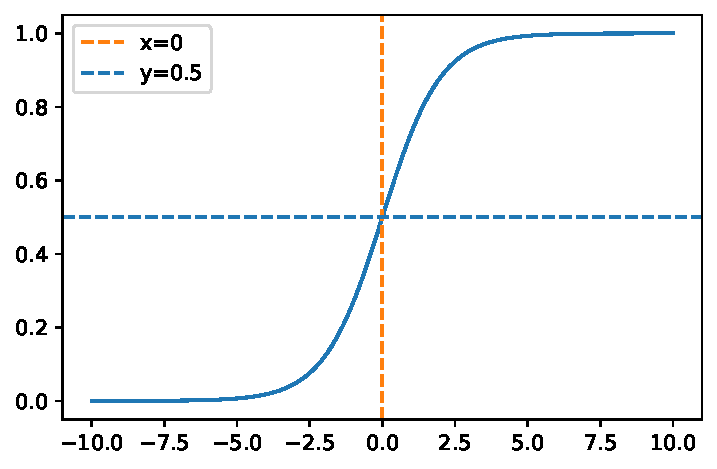
\includegraphics[keepaspectratio]{contents/1/logistic_files/figure-pdf/cell-2-output-1.pdf}}

\begin{tcolorbox}[enhanced jigsaw, arc=.35mm, bottomrule=.15mm, bottomtitle=1mm, breakable, colback=white, colbacktitle=quarto-callout-note-color!10!white, colframe=quarto-callout-note-color-frame, coltitle=black, left=2mm, leftrule=.75mm, opacityback=0, opacitybacktitle=0.6, rightrule=.15mm, title=\textcolor{quarto-callout-note-color}{\faInfo}\hspace{0.5em}{Historical Note}, titlerule=0mm, toprule=.15mm, toptitle=1mm]

The logistic curve was introduced by Pierre-François Verhulst in 1838
{[}5{]} while studying population growth.

The term \textbf{logit} was introduced by Joseph Berkson in 1944
{[}6{]}. Berkson used the word logit for the logarithm of the odds and
advocated the logistic function in bioassay problems.

Logistic regression later became a central example of generalized linear
models. In GLM terminology, logistic regression uses:

\begin{itemize}
\tightlist
\item
  Bernoulli response distribution;
\item
  logit link function;
\item
  linear predictor \(x^\top\beta\).
\end{itemize}

\end{tcolorbox}

\subsection{Logistic Regression as a Linear
Classifier}\label{logistic-regression-as-a-linear-classifier}

Logistic regression produces probabilities, therefore it can also be
used for classification.

Using the common threshold \(t=0.5\), we predict

\[
\hat y
=
\begin{cases}
1,& p(x)\ge 0.5,\\
0,& p(x)<0.5.
\end{cases}
\]

Since

\[
p(x)\ge 0.5
\iff
x^\top\beta\ge 0,
\]

the classification rule becomes

\[
\hat y
=
\begin{cases}
1,& x^\top\beta\ge 0,\\
0,& x^\top\beta<0.
\end{cases}
\]

Therefore, the decision boundary is

\[
x^\top\beta=0.
\]

\begin{tcolorbox}[enhanced jigsaw, arc=.35mm, bottomrule=.15mm, bottomtitle=1mm, breakable, colback=white, colbacktitle=quarto-callout-note-color!10!white, colframe=quarto-callout-note-color-frame, coltitle=black, left=2mm, leftrule=.75mm, opacityback=0, opacitybacktitle=0.6, rightrule=.15mm, title=\textcolor{quarto-callout-note-color}{\faInfo}\hspace{0.5em}{Geometric Interpretation}, titlerule=0mm, toprule=.15mm, toptitle=1mm]

The decision boundary \(x^\top\beta=0\) is a line in two dimensions, a
plane in three dimensions, and a hyperplane in higher dimensions.

Thus logistic regression is a linear classifier: Even though the
probability curve is nonlinear, the decision boundary is linear in the
original predictor space.

\end{tcolorbox}

\subsection{Interpreting the
Coefficients}\label{interpreting-the-coefficients}

Consider the model \[
p(x)=\sigma(\beta_0+\beta_1x_1+\ldots+\beta_px_p),
\] where \(\beta_0+\beta_1x_1+\ldots+\beta_px_p=x^\top \beta\) is the
linear predictor.

Suppose all other predictors are held fixed. Increasing \(x_j\) by one
unit changes the linear predictor by \(\beta_j\). Because the linear
predictor represents the log-odds, increasing \(x_j\) by one unit
changes the log-odds by \(\beta_j\).

Thus:

\begin{itemize}
\tightlist
\item
  if \(\beta_j>0\), increasing \(x_j\) increases the log-odds of class
  \(1\);
\item
  if \(\beta_j<0\), increasing \(x_j\) decreases the log-odds of class
  \(1\);
\item
  if \(\beta_j=0\), increasing \(x_j\) does not change the log-odds.
\end{itemize}

For a one-unit increase in \(x_j\), holding all other predictors fixed,
the linear predictor increases by \(\beta_j\). Since \(\beta_j\) is a
change in log-odds, exponentiating gives a multiplicative change in
odds, then the odds are expected to be multiplied by \(\exp(\beta_j)\):

Consider \[
\log(\text{odds}_1)-\log(\text{odds}_2)=\beta_j.
\] Then \[
\frac{\text{odds}_1}{\text{odds}_2}=\me^{\beta_j}.
\]

\begin{definition}[Odds
Ratio]\protect\hypertarget{def-odds-ratio}{}\label{def-odds-ratio}

The quantity \(\exp(\beta_j)\) is called the \textbf{odds ratio}.

\end{definition}

\begin{example}[Example]\protect\hypertarget{exm-}{}\label{exm-}

Suppose \(\beta_j=0.08\). Since

\[
\exp(0.08)\approx 1.083,
\] Then a one-unit increase in \(x_j\) multiplies the odds by
approximately \(1.083\). Equivalently, the odds increase by
approximately \(8.3\%\).

\end{example}

\begin{tcolorbox}[enhanced jigsaw, arc=.35mm, bottomrule=.15mm, bottomtitle=1mm, breakable, colback=white, colbacktitle=quarto-callout-note-color!10!white, colframe=quarto-callout-note-color-frame, coltitle=black, left=2mm, leftrule=.75mm, opacityback=0, opacitybacktitle=0.6, rightrule=.15mm, title=\textcolor{quarto-callout-note-color}{\faInfo}\hspace{0.5em}{Note}, titlerule=0mm, toprule=.15mm, toptitle=1mm]

The coefficient \(\beta_j\) is not a direct change in probability since
the relation between the logit and the probability is a sigmoid function
(which is non-linear). So the probability change depends on the current
value of \(x^\top\beta\). For the same value of \(\beta_j\), the
probability change can be small when \(p(x)\) is already close to \(0\)
or close to \(1\), and larger when \(p(x)\) is near \(0.5\).

\end{tcolorbox}

\section{Maximum Likelihood
Estimation}\label{maximum-likelihood-estimation}

Logistic regression is usually fit using maximum likelihood estimation.

Assume we are given a dataset \(\qty{(x_i,y_i)}_{i=1}^n\), where
\(y_i\in\qty{0,1}\). In logistic regression, we model the conditional
probability that the response belongs to class \(1\): \[
p_i=\Pr(Y_i=1\mid X_i=x_i)=\sigma(x_i^\top\beta).
\]

Since \(Y_i\) only takes the values \(0\) and \(1\), it is natural to
model its conditional distribution using a Bernoulli distribution. \[
Y_i\mid X_i=x_i\sim\operatorname{Bernoulli}(p_i).
\]

The probability mass function of a Bernoulli random variable is

\[
\Pr(Y_i=y_i)
=
p_i^{y_i}(1-p_i)^{1-y_i}.
\]

Assuming the observations are independent and conditional on the
predictors, the likelihood function is

\[
L(\beta)
=
\prod_{i=1}^{n}
p_i^{y_i}(1-p_i)^{1-y_i}.
\]

Taking the logarithm, the log-likelihood is

\[
\ell(\beta)=\sum_{i=1}^{n}\qty[y_i\log(p_i)+(1-y_i)\log(1-p_i)].
\]

The maximum likelihood estimate is

\[
\hat\beta
=
\arg\max_{\beta}\ell(\beta).
\]

\begin{tcolorbox}[enhanced jigsaw, arc=.35mm, bottomrule=.15mm, bottomtitle=1mm, breakable, colback=white, colbacktitle=quarto-callout-note-color!10!white, colframe=quarto-callout-note-color-frame, coltitle=black, left=2mm, leftrule=.75mm, opacityback=0, opacitybacktitle=0.6, rightrule=.15mm, title=\textcolor{quarto-callout-note-color}{\faInfo}\hspace{0.5em}{Gradient descent}, titlerule=0mm, toprule=.15mm, toptitle=1mm]

Unlike ordinary least squares, logistic regression does not have a
simple closed-form solution for \(\hat\beta\). In practice, numerical
optimization methods are used.

Gradient descent is one of the most widely used optimization methods in
machine learning. Although linear regression and logistic regression use
different models and different loss functions, their gradient
expressions have a similar matrix form. As a result, their gradient
descent update formulas also look very similar.

Gradient descent is beyond the scope of this course, although it plays
an important role in modern machine learning.

\end{tcolorbox}

\subsection{Binary Cross-Entropy and a Single
Neuron}\label{binary-cross-entropy-and-a-single-neuron}

The negative log-likelihood is

\[
-\ell(\beta)
=
-\sum_{i=1}^{n}
\left[
y_i\log(p_i)
+
(1-y_i)\log(1-p_i)
\right].
\]

In machine learning, this is called binary cross-entropy loss or log
loss. It is simply the negative of the log-likelihood mentioned in the
previous section. The reason of this negative is that in machine
learning it is usually preferred to lower the loss function.

Therefore logistic regression is not just a classification model. It is
also a probabilistic model trained by minimizing a loss function that
rewards accurate probability estimates.

What is more, a logistic regression model can be viewed as a single
sigmoid neuron, since the model has the form

\[
x
\longmapsto
x^\top\beta
\longmapsto
\sigma(x^\top\beta)
\longmapsto
p(x).
\]

This is essentially a neural network with no hidden layers and one
output unit, with sigmoid activation and binary cross-entropy loss.

This connects logistic regression to modern machine learning methods,
including neural networks, which often use cross-entropy loss for
classification.

\section{Regularized Logistic
Regression}\label{regularized-logistic-regression}

When there are many predictors, logistic regression can overfit. A
common solution is to add regularization, like ridge and lasso for
linear regression.

\begin{enumerate}
\def\labelenumi{\arabic{enumi}.}
\tightlist
\item
  Ridge logistic regression penalizes large coefficients using an
  \(L^2\) penalty:
\end{enumerate}

\[
-\ell(\beta)
+
\lambda\sum_{j=1}^{p}\beta_j^2.
\] This shrinks coefficients toward zero but usually does not set them
exactly to zero.

\begin{enumerate}
\def\labelenumi{\arabic{enumi}.}
\setcounter{enumi}{1}
\tightlist
\item
  Lasso logistic regression uses an \(L^1\) penalty:
\end{enumerate}

\[
-\ell(\beta)
+
\lambda\sum_{j=1}^{p}|\beta_j|.
\] This can shrink some coefficients exactly to zero, producing a
simpler model.

\section{\texorpdfstring{Logistic Regression in
\texttt{sklearn}}{Logistic Regression in sklearn}}\label{logistic-regression-in-sklearn}

We usually use \texttt{LogisticRegression} from
\texttt{sklearn.linear\_model} to implement logistic regression. The
most commonly used solver in modern versions of scikit-learn is
\texttt{lbfgs}, which is the default choice for
\texttt{LogisticRegression()}. It is a quasi-Newton optimization method
that usually converges much faster than simple gradient descent. In
addition it is automatically extended to multiclass cases.

The basic code is as usual:

\begin{Shaded}
\begin{Highlighting}[]
\ImportTok{from}\NormalTok{ sklearn.pipeline }\ImportTok{import}\NormalTok{ make\_pipeline}
\ImportTok{from}\NormalTok{ sklearn.preprocessing }\ImportTok{import}\NormalTok{ StandardScaler}
\ImportTok{from}\NormalTok{ sklearn.linear\_model }\ImportTok{import}\NormalTok{ LogisticRegression}

\NormalTok{logit }\OperatorTok{=}\NormalTok{ make\_pipeline(}
\NormalTok{    StandardScaler(),}
\NormalTok{    LogisticRegression(max\_iter}\OperatorTok{=}\DecValTok{5000}\NormalTok{),}
\NormalTok{)}

\NormalTok{logit.fit(X\_train, y\_train)}

\NormalTok{test\_prob }\OperatorTok{=}\NormalTok{ logit.predict\_proba(X\_test)}
\NormalTok{test\_pred }\OperatorTok{=}\NormalTok{ logit.predict(X\_test)}
\end{Highlighting}
\end{Shaded}

Logistic regression is very similar to linear regression, that the
scales of features matters. Therefore we need to set up a pipeline to
standarize al features first.

The model actually has two types of outputs:

\begin{itemize}
\tightlist
\item
  \texttt{predict\_proba()} returns estimated class probabilities. The
  second column is the estimated probability of the positive class.
\item
  \texttt{predict()} returns class labels using the default threshold
  \(0.5\).
\end{itemize}

\subsection{Regularization}\label{regularization-1}

The general idea of regularization in \texttt{LogisticRegression()} is
based on the elastic-net style penalty, which is controlled by two
arguments \texttt{l1\_ratio} and \texttt{C}. Conceptually, the penalty
behaves like \[
-\ell+\frac1C(\verb|l1_ratio|\norm{\beta}_1+(1-\verb|l1_ratio|)\norm{\beta}_2^2).
\]

\begin{itemize}
\tightlist
\item
  \texttt{l1\_ratio} is to control the type of regularization:

  \begin{itemize}
  \tightlist
  \item
    \texttt{l1\_ratio\ =\ 0}: pure L2 regularization;
  \item
    \texttt{l1\_ratio\ =\ 1}: pure L1 regularization;
  \item
    \texttt{0\ \textless{}\ l1\_ratio\ \textless{}\ 1}: elastic-net
    regularization.
  \end{itemize}
\item
  \texttt{C}, which is \(1/\lambda\), is to control the regularization
  strength:

  \begin{itemize}
  \tightlist
  \item
    \texttt{C=np.inf} means no penalty.
  \end{itemize}
\end{itemize}

The exact formula used inside \texttt{sklearn} is more complicated which
incorprates other aspects such as number of observations.

Note that some combinations of regularization and solvers are not
compatible. For example,

\begin{itemize}
\tightlist
\item
  elastic-net regularization requires the \texttt{saga} solver;
\item
  the default solve \texttt{lbfgs} requires \texttt{l2} so
  \texttt{l1\_ratio} has to be 0.
\end{itemize}

The default setting for \texttt{LogisticRegression()} is that
\texttt{l1\_ratio=0}, \texttt{C=1} and \texttt{solver="lbfgs"}.

\section{Example 1: Binary
classification}\label{example-1-binary-classification}

We first consider a binary classification problem.

The Titanic dataset records information about passengers aboard the
Titanic. Our goal is to predict whether a passenger survived. We load
the dataset from the database from \texttt{seaborn}.

\begin{Shaded}
\begin{Highlighting}[]
\ImportTok{import}\NormalTok{ seaborn }\ImportTok{as}\NormalTok{ sns}
\ImportTok{from}\NormalTok{ sklearn.model\_selection }\ImportTok{import}\NormalTok{ train\_test\_split}

\NormalTok{titanic }\OperatorTok{=}\NormalTok{ sns.load\_dataset(}\StringTok{"titanic"}\NormalTok{)}
\NormalTok{data }\OperatorTok{=}\NormalTok{ titanic[[}\StringTok{"survived"}\NormalTok{, }\StringTok{"age"}\NormalTok{, }\StringTok{"fare"}\NormalTok{, }\StringTok{"pclass"}\NormalTok{]].dropna()}
\NormalTok{X }\OperatorTok{=}\NormalTok{ data[[}\StringTok{"age"}\NormalTok{, }\StringTok{"fare"}\NormalTok{, }\StringTok{"pclass"}\NormalTok{]]}
\NormalTok{y }\OperatorTok{=}\NormalTok{ data[}\StringTok{"survived"}\NormalTok{]}
\NormalTok{X\_train, X\_test, y\_train, y\_test }\OperatorTok{=}\NormalTok{ train\_test\_split(}
\NormalTok{    X, y, test\_size}\OperatorTok{=}\FloatTok{0.3}\NormalTok{, stratify}\OperatorTok{=}\NormalTok{y, random\_state}\OperatorTok{=}\DecValTok{1}
\NormalTok{)}
\end{Highlighting}
\end{Shaded}

Here we only use 3 features \texttt{age}, \texttt{fare} and
\texttt{pclass} to predict \texttt{survived}.

We quickly fit the model with default setting.

\protect\phantomsection\label{annotated-cell-112}%
\begin{Shaded}
\begin{Highlighting}[]
\ImportTok{from}\NormalTok{ sklearn.pipeline }\ImportTok{import}\NormalTok{ make\_pipeline}
\ImportTok{from}\NormalTok{ sklearn.preprocessing }\ImportTok{import}\NormalTok{ StandardScaler}
\ImportTok{from}\NormalTok{ sklearn.linear\_model }\ImportTok{import}\NormalTok{ LogisticRegression}

\NormalTok{logit }\OperatorTok{=}\NormalTok{ make\_pipeline(StandardScaler(), LogisticRegression(max\_iter}\OperatorTok{=}\DecValTok{5000}\NormalTok{))}
\NormalTok{logit.fit(X\_train, y\_train)}
\NormalTok{test\_prob }\OperatorTok{=}\NormalTok{ logit.predict\_proba(X\_test)[:, }\DecValTok{1}\NormalTok{] }\CommentTok{\# \textless{}1\textgreater{}}
\NormalTok{test\_pred }\OperatorTok{=}\NormalTok{ logit.predict(X\_test)}
\end{Highlighting}
\end{Shaded}

\begin{description}
\tightlist
\item[5CB6E08D-list-annote-1]
For binary classification, the output of \texttt{.predict\_proba()}
contains two columns, each for a class. We want to test 1, so we choose
column 1.
\end{description}

We focus on tuning \texttt{C} and the threshold. Note that the two
hyperparameters take effects in different stage. \texttt{C} is about the
training of the model, while the threshold is about prediction.
Therefore for logistic regression we usually tune \texttt{C} first and
then find the best threshold afterwards.

\subsection{\texorpdfstring{Tuning
\texttt{C}}{Tuning C}}\label{tuning-c}

We use cross-validation with the F1 score as the evaluation metric.
Since the F1 score combines precision and recall, it is useful when we
want to balance false positives and false negatives. In this example, we
use it to select a model that balances the two types of classification
errors when predicting passenger survival.

\begin{Shaded}
\begin{Highlighting}[]
\ImportTok{import}\NormalTok{ numpy }\ImportTok{as}\NormalTok{ np}
\ImportTok{from}\NormalTok{ sklearn.model\_selection }\ImportTok{import}\NormalTok{ GridSearchCV}

\NormalTok{param\_grid }\OperatorTok{=}\NormalTok{ \{}\StringTok{"logisticregression\_\_C"}\NormalTok{: np.logspace(}\OperatorTok{{-}}\DecValTok{3}\NormalTok{, }\DecValTok{3}\NormalTok{, }\DecValTok{20}\NormalTok{)\}}
\NormalTok{grid }\OperatorTok{=}\NormalTok{ GridSearchCV(logit, param\_grid}\OperatorTok{=}\NormalTok{param\_grid, cv}\OperatorTok{=}\DecValTok{5}\NormalTok{, scoring}\OperatorTok{=}\StringTok{"f1"}\NormalTok{)}
\NormalTok{grid.fit(X\_train, y\_train)}
\NormalTok{grid.best\_params\_}
\end{Highlighting}
\end{Shaded}

\begin{verbatim}
{'logisticregression__C': np.float64(2.976351441631316)}
\end{verbatim}

\subsection{Tuning the threshold}\label{tuning-the-threshold}

To tune the threshold, we use the helper function defined in
Chapter~\ref{sec-cla_dec}.

\begin{Shaded}
\begin{Highlighting}[]
\ImportTok{from}\NormalTok{ sklearn.metrics }\ImportTok{import}\NormalTok{ accuracy\_score, precision\_score, recall\_score, f1\_score}
\ImportTok{from}\NormalTok{ sklearn.metrics }\ImportTok{import}\NormalTok{ confusion\_matrix}

\KeywordTok{def}\NormalTok{ classification\_summary(y\_true, prob, threshold}\OperatorTok{=}\FloatTok{0.5}\NormalTok{):}
\NormalTok{    pred }\OperatorTok{=}\NormalTok{ (prob }\OperatorTok{\textgreater{}=}\NormalTok{ threshold).astype(}\BuiltInTok{int}\NormalTok{)}
\NormalTok{    TN, FP, FN, TP }\OperatorTok{=}\NormalTok{ confusion\_matrix(y\_true, pred).ravel()}

    \ControlFlowTok{return}\NormalTok{ \{}
        \StringTok{"threshold"}\NormalTok{: threshold,}
        \StringTok{"TP"}\NormalTok{: TP,}
        \StringTok{"FP"}\NormalTok{: FP,}
        \StringTok{"FN"}\NormalTok{: FN,}
        \StringTok{"TN"}\NormalTok{: TN,}
        \StringTok{"accuracy"}\NormalTok{: accuracy\_score(y\_true, pred),}
        \StringTok{"precision"}\NormalTok{: precision\_score(y\_true, pred, zero\_division}\OperatorTok{=}\DecValTok{0}\NormalTok{),}
        \StringTok{"recall"}\NormalTok{: recall\_score(y\_true, pred, zero\_division}\OperatorTok{=}\DecValTok{0}\NormalTok{),}
        \StringTok{"f1"}\NormalTok{: f1\_score(y\_true, pred, zero\_division}\OperatorTok{=}\DecValTok{0}\NormalTok{),}
\NormalTok{    \}}
\end{Highlighting}
\end{Shaded}

We may use the regular split-validation method. The model use the best
\texttt{C} from the cross-validation from the previous section.

\protect\phantomsection\label{annotated-cell-115}%
\begin{Shaded}
\begin{Highlighting}[]
\ImportTok{from}\NormalTok{ sklearn.model\_selection }\ImportTok{import}\NormalTok{ train\_test\_split}
\ImportTok{import}\NormalTok{ pandas }\ImportTok{as}\NormalTok{ pd}

\NormalTok{X\_model, X\_valid, y\_model, y\_valid }\OperatorTok{=}\NormalTok{ train\_test\_split(}
\NormalTok{    X\_train, y\_train, test\_size}\OperatorTok{=}\FloatTok{0.25}\NormalTok{, stratify}\OperatorTok{=}\NormalTok{y\_train, random\_state}\OperatorTok{=}\DecValTok{1}
\NormalTok{)}

\NormalTok{best\_C }\OperatorTok{=}\NormalTok{ grid.best\_params\_[}\StringTok{\textquotesingle{}logisticregression\_\_C\textquotesingle{}}\NormalTok{]}

\NormalTok{candidate\_thresholds }\OperatorTok{=}\NormalTok{ np.linspace(}\FloatTok{0.05}\NormalTok{, }\FloatTok{0.95}\NormalTok{, }\DecValTok{91}\NormalTok{)}

\NormalTok{results }\OperatorTok{=}\NormalTok{ []}
\ControlFlowTok{for}\NormalTok{ t }\KeywordTok{in}\NormalTok{ candidate\_thresholds:}
\NormalTok{    best\_logit }\OperatorTok{=}\NormalTok{ make\_pipeline(}
\NormalTok{        StandardScaler(),}
\NormalTok{        LogisticRegression(C}\OperatorTok{=}\NormalTok{best\_C, max\_iter}\OperatorTok{=}\DecValTok{5000}\NormalTok{),}
\NormalTok{    )}
\NormalTok{    best\_logit.fit(X\_model, y\_model)}
\NormalTok{    valid\_prob }\OperatorTok{=}\NormalTok{ best\_logit.predict\_proba(X\_valid)[:, }\DecValTok{1}\NormalTok{]}
\NormalTok{    results.append(classification\_summary(y\_valid, valid\_prob, threshold}\OperatorTok{=}\NormalTok{t))}

\NormalTok{threshold\_df }\OperatorTok{=}\NormalTok{ pd.DataFrame(results)}

\NormalTok{best\_row }\OperatorTok{=}\NormalTok{ threshold\_df.loc[threshold\_df[}\StringTok{"f1"}\NormalTok{].idxmax()] }\CommentTok{\# \textless{}1\textgreater{}}
\NormalTok{best\_row}
\end{Highlighting}
\end{Shaded}

\begin{description}
\tightlist
\item[5CB6E08D-list-annote-1]
\texttt{best\_row} is a Series object. Therefore although it is a row,
it is displayed as a column.
\end{description}

\begin{verbatim}
threshold     0.360000
TP           39.000000
FP           17.000000
FN           12.000000
TN           57.000000
accuracy      0.768000
precision     0.696429
recall        0.764706
f1            0.728972
Name: 31, dtype: float64
\end{verbatim}

We can fix the threshold and treat it as part of the prediction rule.

\begin{Shaded}
\begin{Highlighting}[]
\ImportTok{from}\NormalTok{ sklearn.model\_selection }\ImportTok{import}\NormalTok{ FixedThresholdClassifier}

\NormalTok{final\_logit }\OperatorTok{=}\NormalTok{ make\_pipeline(}
\NormalTok{    StandardScaler(), LogisticRegression(C}\OperatorTok{=}\NormalTok{best\_C, max\_iter}\OperatorTok{=}\DecValTok{5000}\NormalTok{)}
\NormalTok{)}
\NormalTok{model\_with\_threshold }\OperatorTok{=}\NormalTok{ FixedThresholdClassifier(}
\NormalTok{    final\_logit, threshold}\OperatorTok{=}\NormalTok{best\_row[}\StringTok{"threshold"}\NormalTok{]}
\NormalTok{)}
\NormalTok{model\_with\_threshold.fit(X\_train, y\_train)}
\NormalTok{model\_with\_threshold.score(X\_test, y\_test)}
\end{Highlighting}
\end{Shaded}

\begin{verbatim}
0.6465116279069767
\end{verbatim}

\begin{tcolorbox}[enhanced jigsaw, arc=.35mm, bottomrule=.15mm, bottomtitle=1mm, breakable, colback=white, colbacktitle=quarto-callout-note-color!10!white, colframe=quarto-callout-note-color-frame, coltitle=black, left=2mm, leftrule=.75mm, opacityback=0, opacitybacktitle=0.6, rightrule=.15mm, title=\textcolor{quarto-callout-note-color}{\faInfo}\hspace{0.5em}{Note}, titlerule=0mm, toprule=.15mm, toptitle=1mm]

Notice that changing the threshold does not change the fitted model. The
estimated probabilities remain the same. The threshold only changes how
those probabilities are converted into class labels.

\end{tcolorbox}

\section{Multiclass Extension}\label{multiclass-extension}

The basic logistic regression model handles binary outcomes. For
problems with more than two classes, a common extension is multinomial
logistic regression.

Suppose

\[
Y\in{1,2,\ldots,K}.
\]

Instead of modeling the probability of a single class, multinomial
logistic regression models the probability of every class
simultaneously.

For each class \(k\), define a linear predictor

\[
\eta_k(x)=x^\top\beta_k=\beta_{0,k}+\beta_{1,k}x_1+\ldots+\beta_{p,k}x_p.
\]

The predicted probability of class \(k\) is then given by the softmax
function:

\[
\Pr(Y=k\mid X=x)=
\frac{\exp(\eta_k(x))}
{\sum_{\ell=1}^{K}\exp(\eta_\ell(x))}.
\]

The softmax function converts the collection of scores

\[
\eta_1(x),\eta_2(x),\ldots,\eta_K(x)
\]

into probabilities that satisfy

\[
0\le \Pr(Y=k\mid X=x)\le 1
\]

and

\[
\sum_{k=1}^{K}\Pr(Y=k\mid X=x)=1.
\]

The softmax function plays the same role in multiclass classification
that the sigmoid function plays in binary classification.

\begin{tcolorbox}[enhanced jigsaw, arc=.35mm, bottomrule=.15mm, bottomtitle=1mm, breakable, colback=white, colbacktitle=quarto-callout-note-color!10!white, colframe=quarto-callout-note-color-frame, coltitle=black, left=2mm, leftrule=.75mm, opacityback=0, opacitybacktitle=0.6, rightrule=.15mm, title=\textcolor{quarto-callout-note-color}{\faInfo}\hspace{0.5em}{Note}, titlerule=0mm, toprule=.15mm, toptitle=1mm]

For K=2 classes, softmax reduces to the sigmoid model.

\end{tcolorbox}

For prediction, the observation is assigned to the class with the
largest predicted probability:

\[
\hat y=\arg\max_k P(Y=k\mid X=x).
\]

\subsection{Cross-Entropy Loss}\label{cross-entropy-loss}

Suppose the true class labels are represented using one-hot encoding:

\[
y_{ik}=
\begin{cases}
1,&\text{if observation }i\text{ belongs to class }k,\\
0,&\text{otherwise}.
\end{cases}
\]

Let

\[
p_{ik}=P(Y_i=k\mid X_i=x_i)
\]

denote the predicted probability from the softmax model.

The multiclass cross-entropy loss is

\[
L=-\sum_{i=1}^{n}\sum_{k=1}^{K}y_{ik}\log(p_{ik}).
\]

Because exactly one value of \(y_{ik}\) equals \(1\) for each
observation, this loss simply penalizes the model when it assigns a low
probability to the true class.

Minimizing the multiclass cross-entropy loss is equivalent to maximizing
the likelihood of the multinomial logistic regression model, just as
binary cross-entropy corresponds to maximum likelihood estimation in
ordinary logistic regression.

\begin{tcolorbox}[enhanced jigsaw, arc=.35mm, bottomrule=.15mm, bottomtitle=1mm, breakable, colback=white, colbacktitle=quarto-callout-note-color!10!white, colframe=quarto-callout-note-color-frame, coltitle=black, left=2mm, leftrule=.75mm, opacityback=0, opacitybacktitle=0.6, rightrule=.15mm, title=\textcolor{quarto-callout-note-color}{\faInfo}\hspace{0.5em}{One-vs-Rest (OvR)}, titlerule=0mm, toprule=.15mm, toptitle=1mm]

Another approach to multiclass classification is One-vs-Rest (OvR), also
called One-vs-All.

Instead of fitting a single multinomial model, OvR trains one binary
classifier for each class. For example, with three classes A, B, and C,
three separate models are fit:

\begin{itemize}
\tightlist
\item
  A versus not A
\item
  B versus not B
\item
  C versus not C
\end{itemize}

The final prediction is usually made using the classifier with the
largest predicted probability.

Although OvR is simple and often works well in practice, multinomial
logistic regression provides a more natural probabilistic model because
all class probabilities are estimated simultaneously and automatically
sum to one.

\end{tcolorbox}

\begin{tcolorbox}[enhanced jigsaw, arc=.35mm, bottomrule=.15mm, bottomtitle=1mm, breakable, colback=white, colbacktitle=quarto-callout-note-color!10!white, colframe=quarto-callout-note-color-frame, coltitle=black, left=2mm, leftrule=.75mm, opacityback=0, opacitybacktitle=0.6, rightrule=.15mm, title=\textcolor{quarto-callout-note-color}{\faInfo}\hspace{0.5em}{\texttt{solver}}, titlerule=0mm, toprule=.15mm, toptitle=1mm]

There are many algorithms for fitting logistic regression models. In
\texttt{scikit-learn}, these optimization algorithms are specified
through the \texttt{solver} argument. Examples include \texttt{"lbfgs"},
\texttt{"newton-cg"}, \texttt{"newton-cholesky"}, \texttt{"sag"},
\texttt{"saga"}, and \texttt{"liblinear"}.

Different solvers use different optimization techniques and may have
different computational properties. Some are better suited for large
datasets, while others are designed for smaller problems or support
additional features such as regularization.

Historically, some solvers handled multiclass classification using a
One-vs-Rest (OvR) strategy, while others directly fit a multinomial
logistic regression model using the softmax formulation.

In this course, we focus on the multinomial (softmax) approach because
it provides a natural extension of binary logistic regression and is
widely used in modern machine learning. The details of optimization
algorithms are beyond the scope of this course.

\end{tcolorbox}

\section{Example 2: Multinomial Logistic
Regression}\label{example-2-multinomial-logistic-regression}

The Titanic example involved two classes. We now consider a multiclass
classification problem using the wine dataset.

\begin{Shaded}
\begin{Highlighting}[]
\ImportTok{from}\NormalTok{ sklearn.datasets }\ImportTok{import}\NormalTok{ load\_wine}
\ImportTok{from}\NormalTok{ sklearn.model\_selection }\ImportTok{import}\NormalTok{ train\_test\_split}

\NormalTok{wine }\OperatorTok{=}\NormalTok{ load\_wine(as\_frame}\OperatorTok{=}\VariableTok{True}\NormalTok{)}

\NormalTok{X }\OperatorTok{=}\NormalTok{ wine.data[[}\StringTok{"alcohol"}\NormalTok{, }\StringTok{"flavanoids"}\NormalTok{, }\StringTok{"color\_intensity"}\NormalTok{]]}
\NormalTok{y }\OperatorTok{=}\NormalTok{ wine.target}

\NormalTok{X\_train, X\_test, y\_train, y\_test }\OperatorTok{=}\NormalTok{ train\_test\_split(}
\NormalTok{    X, y, test\_size}\OperatorTok{=}\FloatTok{0.3}\NormalTok{, stratify}\OperatorTok{=}\NormalTok{y, random\_state}\OperatorTok{=}\DecValTok{1}
\NormalTok{)}
\end{Highlighting}
\end{Shaded}

We fit a multinomial logistic regression model.

\begin{Shaded}
\begin{Highlighting}[]
\ImportTok{from}\NormalTok{ sklearn.pipeline }\ImportTok{import}\NormalTok{ make\_pipeline}
\ImportTok{from}\NormalTok{ sklearn.preprocessing }\ImportTok{import}\NormalTok{ StandardScaler}
\ImportTok{from}\NormalTok{ sklearn.linear\_model }\ImportTok{import}\NormalTok{ LogisticRegression}

\NormalTok{wine\_logit }\OperatorTok{=}\NormalTok{ make\_pipeline(}
\NormalTok{    StandardScaler(),}
\NormalTok{    LogisticRegression(max\_iter}\OperatorTok{=}\DecValTok{5000}\NormalTok{),}
\NormalTok{)}

\NormalTok{wine\_logit.fit(X\_train, y\_train)}

\NormalTok{test\_prob }\OperatorTok{=}\NormalTok{ wine\_logit.predict\_proba(X\_test)}
\NormalTok{test\_pred }\OperatorTok{=}\NormalTok{ wine\_logit.predict(X\_test)}
\end{Highlighting}
\end{Shaded}

\subsection{Probabilities and Softmax}\label{probabilities-and-softmax}

For multiclass problems, logistic regression uses the softmax
formulation discussed earlier.

\begin{Shaded}
\begin{Highlighting}[]
\NormalTok{test\_prob[:}\DecValTok{5}\NormalTok{]}
\end{Highlighting}
\end{Shaded}

\begin{verbatim}
array([[3.32849861e-02, 4.58338942e-02, 9.20881120e-01],
       [7.81045388e-02, 3.03513972e-02, 8.91544064e-01],
       [1.29661355e-02, 5.23981366e-05, 9.86981466e-01],
       [7.03100543e-03, 9.90470483e-01, 2.49851168e-03],
       [3.96520174e-02, 9.59921408e-01, 4.26574383e-04]])
\end{verbatim}

Each row contains the estimated probabilities for all classes. The
probabilities always sum to one.

\begin{Shaded}
\begin{Highlighting}[]
\NormalTok{test\_prob[:}\DecValTok{5}\NormalTok{].}\BuiltInTok{sum}\NormalTok{(axis}\OperatorTok{=}\DecValTok{1}\NormalTok{)}
\end{Highlighting}
\end{Shaded}

\begin{verbatim}
array([1., 1., 1., 1., 1.])
\end{verbatim}

The predicted class is the class with the largest probability.

\begin{Shaded}
\begin{Highlighting}[]
\NormalTok{test\_pred[:}\DecValTok{5}\NormalTok{]}
\end{Highlighting}
\end{Shaded}

\begin{verbatim}
array([2, 2, 2, 1, 1])
\end{verbatim}

Unlike binary logistic regression, there is usually no threshold
parameter to tune. The model simply predicts the class with the highest
probability.

\subsection{Confusion Matrix}\label{confusion-matrix}

\begin{Shaded}
\begin{Highlighting}[]
\ImportTok{from}\NormalTok{ sklearn.metrics }\ImportTok{import}\NormalTok{ ConfusionMatrixDisplay}

\NormalTok{ConfusionMatrixDisplay.from\_predictions(y\_test, test\_pred)}
\end{Highlighting}
\end{Shaded}

\pandocbounded{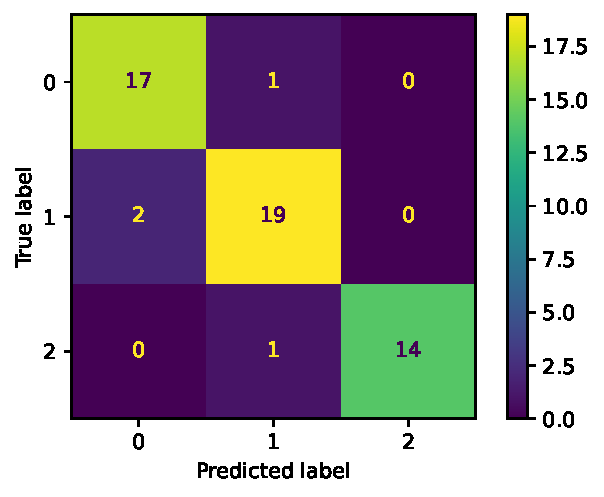
\includegraphics[keepaspectratio]{contents/1/logistic_files/figure-pdf/cell-15-output-1.pdf}}

We could also directly generate the classification report.

\begin{Shaded}
\begin{Highlighting}[]
\ImportTok{from}\NormalTok{ sklearn.metrics }\ImportTok{import}\NormalTok{ classification\_report}

\BuiltInTok{print}\NormalTok{(classification\_report(y\_test, test\_pred))}
\end{Highlighting}
\end{Shaded}

\begin{verbatim}
              precision    recall  f1-score   support

           0       0.89      0.94      0.92        18
           1       0.90      0.90      0.90        21
           2       1.00      0.93      0.97        15

    accuracy                           0.93        54
   macro avg       0.93      0.93      0.93        54
weighted avg       0.93      0.93      0.93        54
\end{verbatim}

The report provides precision, recall, and F1 scores for each class
separately.

\begin{tcolorbox}[enhanced jigsaw, arc=.35mm, bottomrule=.15mm, bottomtitle=1mm, breakable, colback=white, colbacktitle=quarto-callout-note-color!10!white, colframe=quarto-callout-note-color-frame, coltitle=black, left=2mm, leftrule=.75mm, opacityback=0, opacitybacktitle=0.6, rightrule=.15mm, title=\textcolor{quarto-callout-note-color}{\faInfo}\hspace{0.5em}{Note}, titlerule=0mm, toprule=.15mm, toptitle=1mm]

For multiclass logistic regression, the regularization parameter
\texttt{C} can be tuned in the same way as in the binary classification
example.

However, there is usually no single threshold parameter to tune. The
standard prediction rule is to choose the class with the largest
predicted probability.

In this example, we skip the tuning step for \texttt{C} because the
procedure is the same as before.

\end{tcolorbox}

\part{Nonparametric Supervised Learning}

\chapter{K-Nearest Neighbors}\label{k-nearest-neighbors}

K-nearest neighbors (KNN) is a simple nonparametric prediction method.
It does not estimate a fixed formula like linear regression. Instead, it
predicts from nearby training observations. The method is local: points
close to the new observation have influence, and distant points usually
have none.

\section{The KNN Model}\label{the-knn-model}

KNN can be used for both regression and classification. The ideas are
the same: use nearby observations to predict.

\subsection{KNN Regression}\label{knn-regression}

Suppose the training data are \[
\{(x_i,y_i)\}_{i=1}^n,
\quad
x_i\in\mathbb R^p,\; y_i\in\mathbb R.
\]

We want to estimate the regression function

\[
f(x)=\Exp[Y\mid X=x].
\]

\begin{definition}[KNN
regressor]\protect\hypertarget{def-knn-regressor}{}\label{def-knn-regressor}

For a new point \(x_0\), let \(N_K(x_0)\) be the set of indices
corresponding to the \(K\) training points closest to \(x_0\). The KNN
regression estimate is

\[
\hat f(x_0)
=
\frac{1}{K}\sum_{i\in N_K(x_0)} y_i.
\]

That is, the predicted value is the average response among the \(K\)
nearest neighbors of \(x_0\).

KNN regression estimates the conditional mean locally by averaging the
responses of nearby observations.

\end{definition}

Sometimes neighbors are assigned different weights. In that case, a
weighted KNN regressor has the form

\[
\hat f(x_0)
=
\sum_{i=1}^n w_i(x_0)y_i,
\]

where

\[
w_i(x_0)\ge 0,
\qquad
\sum_{i=1}^n w_i(x_0)=1.
\]

Ordinary KNN regression uses

\[
w_i(x_0)
=
\begin{cases}
1/K, & i\in N_K(x_0),\\
0, & i\notin N_K(x_0).
\end{cases}
\]

\subsection{KNN Classification}\label{knn-classification}

For classification, the response is a class label rather than a
numerical response. Given a new point \(x_0\), KNN classification finds
the \(K\) nearest training observations and predicts by majority vote.

\begin{definition}[KNN
classifier]\protect\hypertarget{def-knn-classifier}{}\label{def-knn-classifier}

For a new point \(x_0\), let \(N_K(x_0)\) be the set of indices of the
\(K\) nearest training observations. The KNN classifier predicts

\[
\hat G(x_0)
=
\arg\max_g\sum_{i\in N_K(x_0)}I(y_i=g).
\]

In words, KNN predicts the class receiving the largest number of votes
among the K nearest neighbors.

\end{definition}

For binary classification, KNN naturally provides a local estimate of
the probability that an observation belongs to class 1:

\[
\hat p(x_0)
=
\frac{1}{K}
\sum_{i\in N_K(x_0)} I(y_i=1).
\]

Then predict class 1 if \(\hat p(x_0)\) is larger than a chosen
threshold, usually \(0.5\).

This estimate can be interpreted as the proportion of class-1
observations among the nearest neighbors. The threshold part is related
to logistic regreesion.

\begin{tcolorbox}[enhanced jigsaw, arc=.35mm, bottomrule=.15mm, bottomtitle=1mm, breakable, colback=white, colbacktitle=quarto-callout-note-color!10!white, colframe=quarto-callout-note-color-frame, coltitle=black, left=2mm, leftrule=.75mm, opacityback=0, opacitybacktitle=0.6, rightrule=.15mm, title=\textcolor{quarto-callout-note-color}{\faInfo}\hspace{0.5em}{Note}, titlerule=0mm, toprule=.15mm, toptitle=1mm]

Weighted KNN classification assigns larger weights to some neighbors,
typically those closer to the query point. The predicted class is then
determined by a weighted majority vote.

\end{tcolorbox}

\begin{tcolorbox}[enhanced jigsaw, arc=.35mm, bottomrule=.15mm, bottomtitle=1mm, breakable, colback=white, colbacktitle=quarto-callout-note-color!10!white, colframe=quarto-callout-note-color-frame, coltitle=black, left=2mm, leftrule=.75mm, opacityback=0, opacitybacktitle=0.6, rightrule=.15mm, title=\textcolor{quarto-callout-note-color}{\faInfo}\hspace{0.5em}{Lazy learner}, titlerule=0mm, toprule=.15mm, toptitle=1mm]

Based on the definition, KNN does not estimate model parameters during
training. It mainly stores the training observations and waits until
prediction time to use them. For this reason, KNN is often called a lazy
learner.

The training phase is extremely simple because KNN does not estimate any
model parameters. The algorithm mainly stores the training observations
for later use. If the training data have \(n\) observations and \(p\)
predictors, storing the data costs about \(O(np)\).

The prediction cost can be much higher. For a single new observation, a
brute-force KNN method computes its distance to all \(n\) training
observations. This costs about \(O(np)\). After computing the distances,
the algorithm must identify the \(K\) nearest observations. A full
ranking of all distances requires \(O(n\log n)\) operations, although
more efficient algorithms may reduce this cost. Taking all these into
consideration, if we predict for \(m\) new observations, the brute-force
distance computation costs about \(O(mnp)\).

Thus, KNN is simple to train but can be relatively slow at prediction
time, especially when the training set is large or the number of
predictors is large.

\end{tcolorbox}

\begin{tcolorbox}[enhanced jigsaw, arc=.35mm, bottomrule=.15mm, bottomtitle=1mm, breakable, colback=white, colbacktitle=quarto-callout-note-color!10!white, colframe=quarto-callout-note-color-frame, coltitle=black, left=2mm, leftrule=.75mm, opacityback=0, opacitybacktitle=0.6, rightrule=.15mm, title=\textcolor{quarto-callout-note-color}{\faInfo}\hspace{0.5em}{Comparison with Linear Models}, titlerule=0mm, toprule=.15mm, toptitle=1mm]

Linear models are global models. A single fitted equation is used
throughout the entire predictor space.

KNN is local. The prediction at \(x_0\) is determined by nearby training
observations.

Because of this difference:

\begin{itemize}
\tightlist
\item
  Linear models are simple and interpretable but may fail to capture
  complex nonlinear relationships.
\item
  KNN can adapt to nonlinear patterns without specifying a functional
  form.
\end{itemize}

However, KNN may become unstable when nearby data are sparse or noisy,
while linear models often provide more stable predictions.

\end{tcolorbox}

\subsection{Distance}\label{distance}

The most common distance is Euclidean distance:

\[
d(x,x')
=
\sqrt{\sum_{j=1}^p (x_j-x'_j)^2}.
\]

KNN depends heavily on this distance. If one feature has a much larger
scale than the others, it can dominate the distance calculation. This is
why scaling is usually important.

Although Euclidean distance is the most common choice, other distances
such as Manhattan distance can also be used.

\begin{tcolorbox}[enhanced jigsaw, arc=.35mm, bottomrule=.15mm, bottomtitle=1mm, breakable, colback=white, colbacktitle=quarto-callout-note-color!10!white, colframe=quarto-callout-note-color-frame, coltitle=black, left=2mm, leftrule=.75mm, opacityback=0, opacitybacktitle=0.6, rightrule=.15mm, title=\textcolor{quarto-callout-note-color}{\faInfo}\hspace{0.5em}{Scaling Matters}, titlerule=0mm, toprule=.15mm, toptitle=1mm]

KNN relies entirely on distances between observations.

If one predictor is measured on a much larger scale than another, it can
dominate the distance calculation and effectively determine which
observations are considered neighbors.

For example, a variable measured in thousands may overwhelm another
variable measured between 0 and 1.

Therefore, KNN is usually applied after feature scaling, such as
standardization.

In practice, KNN is often combined with \texttt{StandardScaler()} in a
pipeline.

\end{tcolorbox}

\subsection{\texorpdfstring{The Role of
\(K\)}{The Role of K}}\label{the-role-of-k}

The tuning parameter \(K\) controls the smoothness of the fitted model.

\begin{itemize}
\tightlist
\item
  Small \(K\): uses very local information and can be sensitive to
  noise.
\item
  Large \(K\): averages over more observations and is more stable, but
  can be biased.
\end{itemize}

This is the usual bias-variance tradeoff. Smaller \(K\) produces a more
flexible fit. Larger \(K\) produces a smoother fit.

In practice, \(K\) is typically chosen using cross-validation.

\begin{tcolorbox}[enhanced jigsaw, arc=.35mm, bottomrule=.15mm, bottomtitle=1mm, breakable, colback=white, colbacktitle=quarto-callout-note-color!10!white, colframe=quarto-callout-note-color-frame, coltitle=black, left=2mm, leftrule=.75mm, opacityback=0, opacitybacktitle=0.6, rightrule=.15mm, title=\textcolor{quarto-callout-note-color}{\faInfo}\hspace{0.5em}{Curse of Dimensionality}, titlerule=0mm, toprule=.15mm, toptitle=1mm]

KNN can work well in low-dimensional problems, but it often struggles
when the number of features is large.

In high dimensions, data become sparse. As the number of features
increases, the volume of the feature space grows rapidly. As a result,
observations tend to be far apart from one another. Therefore local
averaging becomes less meaningful.

This is called the curse of dimensionality.

\end{tcolorbox}

\section{\texorpdfstring{KNN in
\texttt{sklearn}}{KNN in sklearn}}\label{knn-in-sklearn}

\texttt{sklearn.neighbors} provides:

\begin{itemize}
\tightlist
\item
  \href{https://scikit-learn.org/stable/modules/generated/sklearn.neighbors.KNeighborsRegressor.html}{\texttt{KNeighborsRegressor}}
  for regression,
\item
  \href{https://scikit-learn.org/stable/modules/generated/sklearn.neighbors.KNeighborsClassifier.html}{\texttt{KNeighborsClassifier}}
  for classification.
\end{itemize}

The estimator interface is the same as other \texttt{sklearn} models:

\begin{enumerate}
\def\labelenumi{\arabic{enumi}.}
\tightlist
\item
  Create the model.
\item
  Fit the model using \texttt{.fit()}.
\item
  Predict using \texttt{.predict()}.
\item
  Usually coupled with \texttt{StandardScaler()} to create a pipeline.
\end{enumerate}

The arguments here are straightforword. In most cases the default choice
(other than \texttt{n\_neighbors} of course) is good enough. For details
please check the official documents.

\section{Example 1: One-Dimensional
Regression}\label{example-1-one-dimensional-regression}

We first simulate a one-dimensional regression problem based on a noisy
sine curve.

\begin{Shaded}
\begin{Highlighting}[]
\ImportTok{import}\NormalTok{ numpy }\ImportTok{as}\NormalTok{ np}
\ImportTok{from}\NormalTok{ sklearn.model\_selection }\ImportTok{import}\NormalTok{ train\_test\_split}

\NormalTok{rng }\OperatorTok{=}\NormalTok{ np.random.default\_rng(}\DecValTok{1}\NormalTok{)}

\NormalTok{N }\OperatorTok{=} \DecValTok{100}
\NormalTok{X }\OperatorTok{=}\NormalTok{ rng.uniform(}\DecValTok{0}\NormalTok{, }\DecValTok{2} \OperatorTok{*}\NormalTok{ np.pi, size}\OperatorTok{=}\NormalTok{N).reshape(}\OperatorTok{{-}}\DecValTok{1}\NormalTok{, }\DecValTok{1}\NormalTok{)}
\NormalTok{y }\OperatorTok{=} \DecValTok{2} \OperatorTok{*}\NormalTok{ np.sin(X[:, }\DecValTok{0}\NormalTok{]) }\OperatorTok{+}\NormalTok{ rng.normal(size}\OperatorTok{=}\NormalTok{N)}

\NormalTok{X\_train, X\_test, y\_train, y\_test }\OperatorTok{=}\NormalTok{ train\_test\_split(X, y, test\_size}\OperatorTok{=}\FloatTok{0.2}\NormalTok{, random\_state}\OperatorTok{=}\DecValTok{1}\NormalTok{)}
\end{Highlighting}
\end{Shaded}

We then generate a grid of values and apply the fitted model to the grid
in order to estimate the underlying regression function.

\begin{Shaded}
\begin{Highlighting}[]
\NormalTok{X\_grid }\OperatorTok{=}\NormalTok{ np.linspace(}\DecValTok{0}\NormalTok{, }\DecValTok{2} \OperatorTok{*}\NormalTok{ np.pi, }\DecValTok{1001}\NormalTok{).reshape(}\OperatorTok{{-}}\DecValTok{1}\NormalTok{, }\DecValTok{1}\NormalTok{)}
\end{Highlighting}
\end{Shaded}

Fit a KNN regressor with \(K=3\).

\begin{Shaded}
\begin{Highlighting}[]
\ImportTok{from}\NormalTok{ sklearn.neighbors }\ImportTok{import}\NormalTok{ KNeighborsRegressor}

\NormalTok{knn }\OperatorTok{=}\NormalTok{ KNeighborsRegressor(n\_neighbors}\OperatorTok{=}\DecValTok{3}\NormalTok{)}
\NormalTok{knn.fit(X\_train, y\_train)}

\NormalTok{y\_grid }\OperatorTok{=}\NormalTok{ knn.predict(X\_grid)}
\end{Highlighting}
\end{Shaded}

Plot the fitted curve.

\begin{Shaded}
\begin{Highlighting}[]
\ImportTok{import}\NormalTok{ matplotlib.pyplot }\ImportTok{as}\NormalTok{ plt}

\NormalTok{plt.scatter(X\_train.ravel(), y\_train, s}\OperatorTok{=}\DecValTok{40}\NormalTok{, label}\OperatorTok{=}\StringTok{"train"}\NormalTok{)}
\NormalTok{plt.scatter(X\_test.ravel(), y\_test, s}\OperatorTok{=}\DecValTok{40}\NormalTok{, marker}\OperatorTok{=}\StringTok{"x"}\NormalTok{, color}\OperatorTok{=}\StringTok{"black"}\NormalTok{, label}\OperatorTok{=}\StringTok{"test"}\NormalTok{)}
\NormalTok{plt.plot(X\_grid.ravel(), y\_grid, color}\OperatorTok{=}\StringTok{"C1"}\NormalTok{)}

\NormalTok{plt.title(}\StringTok{"KNN Regression, K = 3"}\NormalTok{)}
\NormalTok{plt.xlim(}\DecValTok{0}\NormalTok{, }\DecValTok{2} \OperatorTok{*}\NormalTok{ np.pi)}
\NormalTok{plt.legend()}\OperatorTok{;}
\end{Highlighting}
\end{Shaded}

\pandocbounded{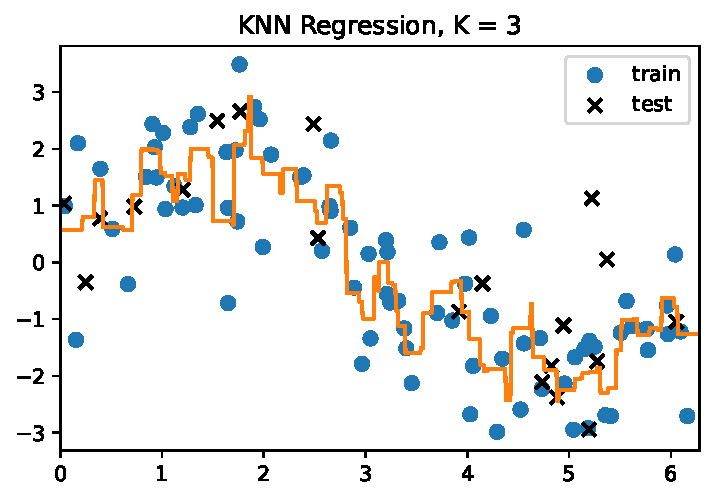
\includegraphics[keepaspectratio]{contents/2/knn_files/figure-pdf/cell-5-output-1.pdf}}

\begin{tcolorbox}[enhanced jigsaw, arc=.35mm, bottomrule=.15mm, bottomtitle=1mm, breakable, colback=white, colbacktitle=quarto-callout-note-color!10!white, colframe=quarto-callout-note-color-frame, coltitle=black, left=2mm, leftrule=.75mm, opacityback=0, opacitybacktitle=0.6, rightrule=.15mm, title=\textcolor{quarto-callout-note-color}{\faInfo}\hspace{0.5em}{The dimension of \texttt{X} and \texttt{X\_grid}}, titlerule=0mm, toprule=.15mm, toptitle=1mm]

Please pay attention to the dimension of \texttt{X} and
\texttt{X\_grid}. We generate them as 2D arrays by
\texttt{.reshape(-1,\ 1)}, and change them back to 1D array in plotting
by \texttt{.ravel()}.

Note that \texttt{.ravel()} is the same as \texttt{.reshape(-1)}. We
choose it because it is shorter.

\end{tcolorbox}

\subsection{\texorpdfstring{Comparing Different Values of
\(K\)}{Comparing Different Values of K}}\label{comparing-different-values-of-k}

The following plot compares several choices of \(K\).

\begin{Shaded}
\begin{Highlighting}[]
\NormalTok{fig, axs }\OperatorTok{=}\NormalTok{ plt.subplots(}\DecValTok{2}\NormalTok{, }\DecValTok{2}\NormalTok{, figsize}\OperatorTok{=}\NormalTok{(}\DecValTok{12}\NormalTok{, }\DecValTok{8}\NormalTok{), sharex}\OperatorTok{=}\VariableTok{True}\NormalTok{, sharey}\OperatorTok{=}\VariableTok{True}\NormalTok{)}

\ControlFlowTok{for}\NormalTok{ ax, k, color }\KeywordTok{in} \BuiltInTok{zip}\NormalTok{(}
\NormalTok{    axs.ravel(),}
\NormalTok{    [}\DecValTok{1}\NormalTok{, }\DecValTok{3}\NormalTok{, }\DecValTok{10}\NormalTok{, }\DecValTok{20}\NormalTok{],}
\NormalTok{    [}\StringTok{"C0"}\NormalTok{, }\StringTok{"C1"}\NormalTok{, }\StringTok{"C2"}\NormalTok{, }\StringTok{"C3"}\NormalTok{],}
\NormalTok{):}
\NormalTok{    model }\OperatorTok{=}\NormalTok{ KNeighborsRegressor(n\_neighbors}\OperatorTok{=}\NormalTok{k)}
\NormalTok{    model.fit(X\_train, y\_train)}
\NormalTok{    pred }\OperatorTok{=}\NormalTok{ model.predict(X\_grid)}

\NormalTok{    ax.scatter(X\_train.ravel(), y\_train, s}\OperatorTok{=}\DecValTok{40}\NormalTok{, label}\OperatorTok{=}\StringTok{"train"}\NormalTok{)}
\NormalTok{    ax.scatter(X\_test.ravel(), y\_test, s}\OperatorTok{=}\DecValTok{40}\NormalTok{, marker}\OperatorTok{=}\StringTok{"x"}\NormalTok{, color}\OperatorTok{=}\StringTok{"black"}\NormalTok{, label}\OperatorTok{=}\StringTok{"test"}\NormalTok{)}
\NormalTok{    ax.plot(X\_grid.ravel(), pred, color}\OperatorTok{=}\NormalTok{color)}
\NormalTok{    ax.set\_title(}\SpecialStringTok{f"K = }\SpecialCharTok{\{}\NormalTok{k}\SpecialCharTok{\}}\SpecialStringTok{"}\NormalTok{)}\OperatorTok{;}
\end{Highlighting}
\end{Shaded}

\pandocbounded{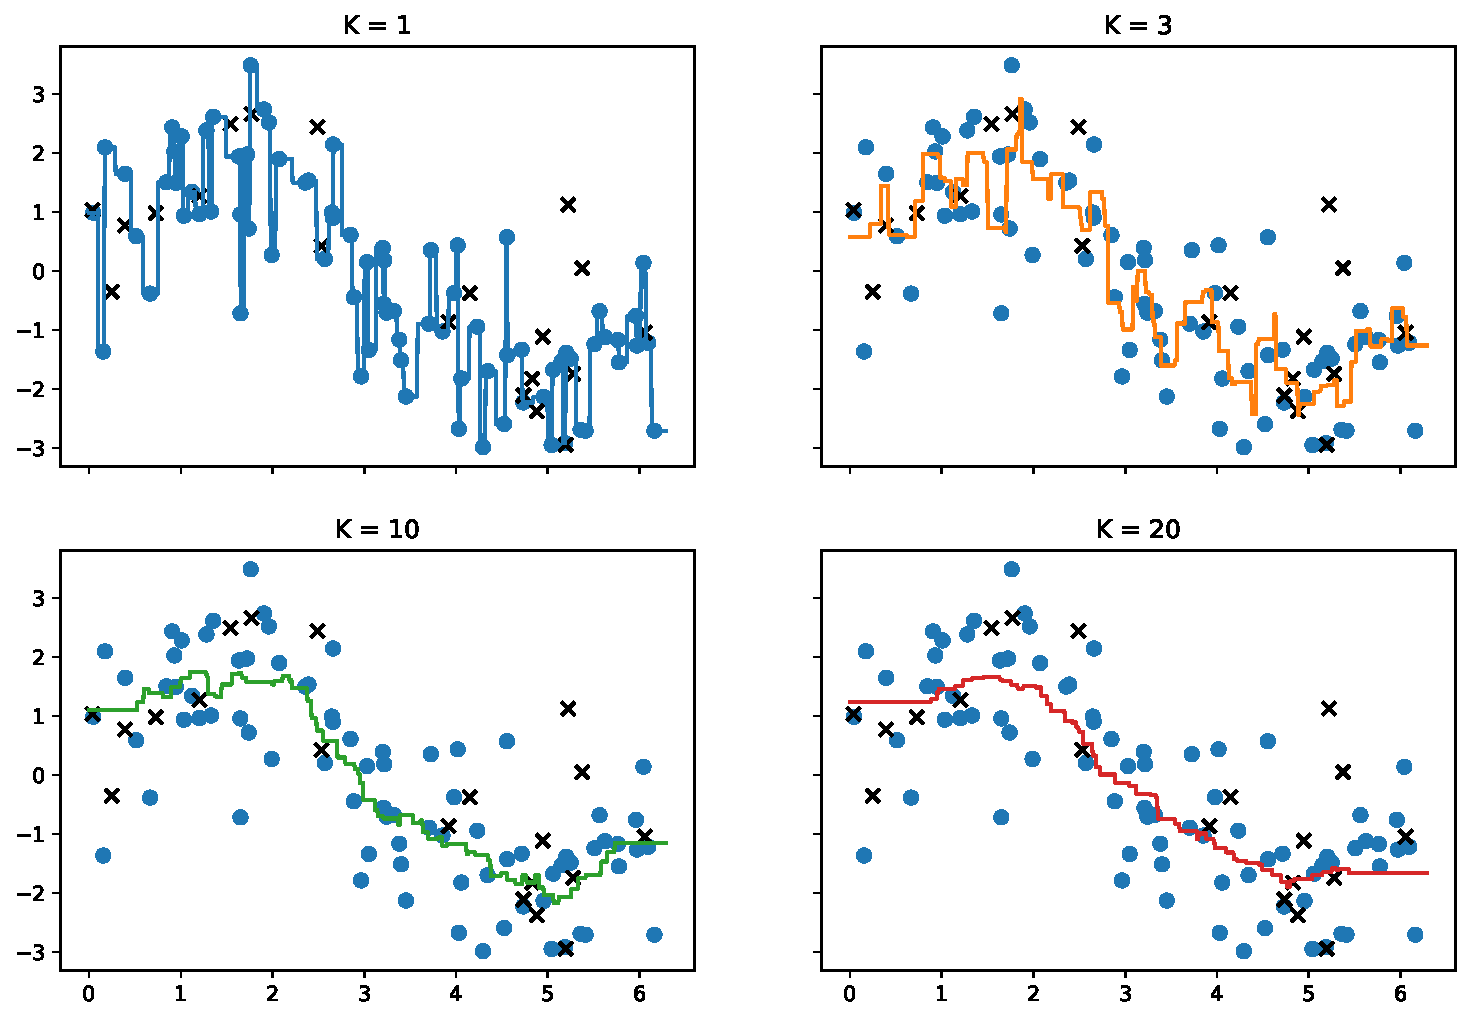
\includegraphics[keepaspectratio]{contents/2/knn_files/figure-pdf/cell-6-output-1.pdf}}

The fitted curve becomes smoother as \(K\) increases.

\subsection{\texorpdfstring{Choosing \(K\) by
Cross-Validation}{Choosing K by Cross-Validation}}\label{choosing-k-by-cross-validation}

We now use cross-validation on the training set to select the value of
\(K\).

Since the training set contains 80 observations and we use
\texttt{cv=5}, each training fold contains only 64 observations.
Therefore we restrict the search range to values of \(K\) that are
safely below this size.

\begin{Shaded}
\begin{Highlighting}[]
\ImportTok{from}\NormalTok{ sklearn.model\_selection }\ImportTok{import}\NormalTok{ GridSearchCV}

\NormalTok{k\_values }\OperatorTok{=} \BuiltInTok{list}\NormalTok{(}\BuiltInTok{range}\NormalTok{(}\DecValTok{1}\NormalTok{, }\DecValTok{61}\NormalTok{))}

\NormalTok{grid }\OperatorTok{=}\NormalTok{ GridSearchCV(KNeighborsRegressor(), param\_grid}\OperatorTok{=}\NormalTok{\{}\StringTok{"n\_neighbors"}\NormalTok{: k\_values\}, cv}\OperatorTok{=}\DecValTok{5}\NormalTok{)}
\NormalTok{grid.fit(X\_train, y\_train)}

\NormalTok{grid.best\_params\_}
\end{Highlighting}
\end{Shaded}

\begin{verbatim}
{'n_neighbors': 26}
\end{verbatim}

Plot the cross-validation score.

\begin{Shaded}
\begin{Highlighting}[]
\NormalTok{plt.plot(k\_values, grid.cv\_results\_[}\StringTok{"mean\_test\_score"}\NormalTok{])}
\NormalTok{plt.axvline(}
\NormalTok{    x}\OperatorTok{=}\NormalTok{grid.best\_params\_[}\StringTok{"n\_neighbors"}\NormalTok{],}
\NormalTok{    color}\OperatorTok{=}\StringTok{"black"}\NormalTok{,}
\NormalTok{    linestyle}\OperatorTok{=}\StringTok{"{-}{-}"}\NormalTok{,}
\NormalTok{)}
\NormalTok{plt.xlabel(}\StringTok{"K"}\NormalTok{)}
\NormalTok{plt.ylabel(}\StringTok{"mean CV score"}\NormalTok{)}
\NormalTok{plt.title(}\SpecialStringTok{f"Cross{-}validation: best K = }\SpecialCharTok{\{}\NormalTok{grid}\SpecialCharTok{.}\NormalTok{best\_params\_[}\StringTok{\textquotesingle{}n\_neighbors\textquotesingle{}}\NormalTok{]}\SpecialCharTok{\}}\SpecialStringTok{"}\NormalTok{)}\OperatorTok{;}
\end{Highlighting}
\end{Shaded}

\pandocbounded{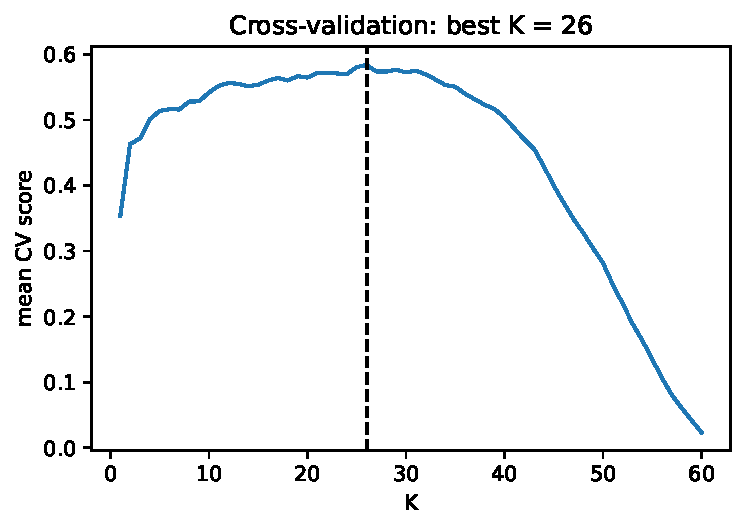
\includegraphics[keepaspectratio]{contents/2/knn_files/figure-pdf/cell-8-output-1.pdf}}

Now plot the fitted curve using the selected value of \(K\).

\begin{Shaded}
\begin{Highlighting}[]
\NormalTok{y\_grid\_best }\OperatorTok{=}\NormalTok{ grid.predict(X\_grid)}

\NormalTok{plt.scatter(X\_train.ravel(), y\_train, s}\OperatorTok{=}\DecValTok{40}\NormalTok{, label}\OperatorTok{=}\StringTok{"train"}\NormalTok{)}
\NormalTok{plt.scatter(X\_test.ravel(), y\_test, s}\OperatorTok{=}\DecValTok{40}\NormalTok{, marker}\OperatorTok{=}\StringTok{"x"}\NormalTok{, color}\OperatorTok{=}\StringTok{"black"}\NormalTok{, label}\OperatorTok{=}\StringTok{"test"}\NormalTok{)}
\NormalTok{plt.plot(X\_grid.ravel(), y\_grid\_best, color}\OperatorTok{=}\StringTok{"C1"}\NormalTok{)}
\NormalTok{plt.title(}\StringTok{"KNN Regression with Cross{-}Validated K"}\NormalTok{)}
\NormalTok{plt.xlim(}\DecValTok{0}\NormalTok{, }\DecValTok{2} \OperatorTok{*}\NormalTok{ np.pi)}\OperatorTok{;}
\end{Highlighting}
\end{Shaded}

\pandocbounded{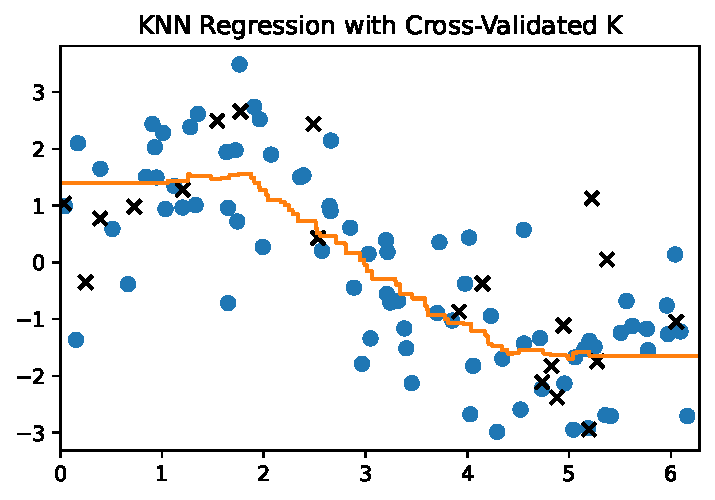
\includegraphics[keepaspectratio]{contents/2/knn_files/figure-pdf/cell-9-output-1.pdf}}

Finally, evaluate the selected model on the test set.

\begin{Shaded}
\begin{Highlighting}[]
\NormalTok{grid.score(X\_test, y\_test)}
\end{Highlighting}
\end{Shaded}

\begin{verbatim}
0.5552931849752354
\end{verbatim}

\section{Example: Iris
Classification}\label{example-iris-classification}

We use the iris data from \texttt{sklearn.datasets}. To make
visualization easy, we use only the first two features: sepal length and
sepal width.

\begin{Shaded}
\begin{Highlighting}[]
\ImportTok{from}\NormalTok{ sklearn }\ImportTok{import}\NormalTok{ datasets}
\ImportTok{from}\NormalTok{ sklearn.model\_selection }\ImportTok{import}\NormalTok{ train\_test\_split}

\NormalTok{iris }\OperatorTok{=}\NormalTok{ datasets.load\_iris()}

\NormalTok{X }\OperatorTok{=}\NormalTok{ iris.data[:, :}\DecValTok{2}\NormalTok{]}
\NormalTok{y }\OperatorTok{=}\NormalTok{ iris.target}

\NormalTok{X\_train, X\_test, y\_train, y\_test }\OperatorTok{=}\NormalTok{ train\_test\_split(}
\NormalTok{    X, y, test\_size}\OperatorTok{=}\FloatTok{0.2}\NormalTok{, random\_state}\OperatorTok{=}\DecValTok{1}\NormalTok{, stratify}\OperatorTok{=}\NormalTok{y}
\NormalTok{)}
\end{Highlighting}
\end{Shaded}

Plot the training data.

\begin{Shaded}
\begin{Highlighting}[]
\NormalTok{fig, ax }\OperatorTok{=}\NormalTok{ plt.subplots(figsize}\OperatorTok{=}\NormalTok{(}\DecValTok{8}\NormalTok{, }\DecValTok{6}\NormalTok{))}

\NormalTok{scatter }\OperatorTok{=}\NormalTok{ ax.scatter(}
\NormalTok{    X\_train[:, }\DecValTok{0}\NormalTok{],}
\NormalTok{    X\_train[:, }\DecValTok{1}\NormalTok{],}
\NormalTok{    c}\OperatorTok{=}\NormalTok{y\_train,}
\NormalTok{    edgecolor}\OperatorTok{=}\StringTok{"k"}\NormalTok{,}
\NormalTok{)}

\NormalTok{labels }\OperatorTok{=}\NormalTok{ [}\StringTok{"setosa"}\NormalTok{, }\StringTok{"versicolor"}\NormalTok{, }\StringTok{"virginica"}\NormalTok{]}
\NormalTok{ax.legend(}
\NormalTok{    handles}\OperatorTok{=}\NormalTok{scatter.legend\_elements()[}\DecValTok{0}\NormalTok{],}
\NormalTok{    labels}\OperatorTok{=}\NormalTok{labels,}
\NormalTok{    title}\OperatorTok{=}\StringTok{"species"}\NormalTok{,}
\NormalTok{)}

\NormalTok{ax.set\_xlabel(iris.feature\_names[}\DecValTok{0}\NormalTok{])}
\NormalTok{ax.set\_ylabel(iris.feature\_names[}\DecValTok{1}\NormalTok{])}
\NormalTok{ax.set\_title(}\StringTok{"Iris Training Data"}\NormalTok{)}
\end{Highlighting}
\end{Shaded}

\begin{verbatim}
Text(0.5, 1.0, 'Iris Training Data')
\end{verbatim}

\pandocbounded{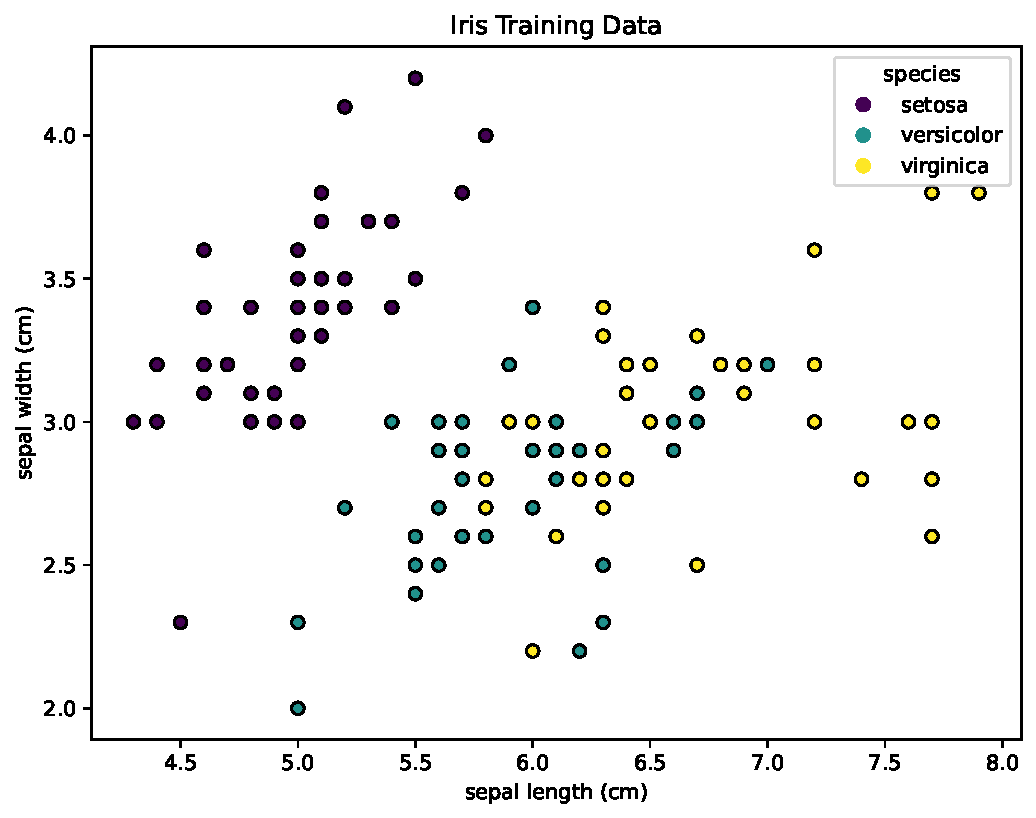
\includegraphics[keepaspectratio]{contents/2/knn_files/figure-pdf/cell-12-output-2.pdf}}

\subsection{Pipeline}\label{pipeline}

The usual KNN workflow includes scaling followed by the KNN model. A
\texttt{Pipeline} keeps these steps together.

\begin{Shaded}
\begin{Highlighting}[]
\ImportTok{from}\NormalTok{ sklearn.pipeline }\ImportTok{import}\NormalTok{ make\_pipeline}
\ImportTok{from}\NormalTok{ sklearn.preprocessing }\ImportTok{import}\NormalTok{ StandardScaler}
\ImportTok{from}\NormalTok{ sklearn.neighbors }\ImportTok{import}\NormalTok{ KNeighborsClassifier}

\NormalTok{pipe }\OperatorTok{=}\NormalTok{ make\_pipeline(StandardScaler(), KNeighborsClassifier(n\_neighbors}\OperatorTok{=}\DecValTok{10}\NormalTok{))}

\NormalTok{pipe.fit(X\_train, y\_train)}
\NormalTok{y\_pred }\OperatorTok{=}\NormalTok{ pipe.predict(X\_test)}
\NormalTok{pipe.score(X\_test, y\_test)}
\end{Highlighting}
\end{Shaded}

\begin{verbatim}
0.7
\end{verbatim}

\subsection{\texorpdfstring{Choosing \(K\) for
Classification}{Choosing K for Classification}}\label{choosing-k-for-classification}

To choose \(K\), we tune \texttt{kneighborsclassifier\_\_n\_neighbors}
inside the pipeline.

\begin{Shaded}
\begin{Highlighting}[]
\ImportTok{from}\NormalTok{ sklearn.model\_selection }\ImportTok{import}\NormalTok{ GridSearchCV}

\NormalTok{n\_values }\OperatorTok{=} \BuiltInTok{list}\NormalTok{(}\BuiltInTok{range}\NormalTok{(}\DecValTok{1}\NormalTok{, }\DecValTok{91}\NormalTok{))}

\NormalTok{param\_grid }\OperatorTok{=}\NormalTok{ \{}\StringTok{"kneighborsclassifier\_\_n\_neighbors"}\NormalTok{: n\_values\}}

\NormalTok{grid }\OperatorTok{=}\NormalTok{ GridSearchCV(pipe, param\_grid}\OperatorTok{=}\NormalTok{param\_grid, cv}\OperatorTok{=}\DecValTok{5}\NormalTok{, scoring}\OperatorTok{=}\StringTok{"accuracy"}\NormalTok{)}

\NormalTok{grid.fit(X\_train, y\_train)}
\NormalTok{grid.best\_params\_}
\end{Highlighting}
\end{Shaded}

\begin{verbatim}
{'kneighborsclassifier__n_neighbors': 5}
\end{verbatim}

The best cross-validation score is:

\begin{Shaded}
\begin{Highlighting}[]
\NormalTok{grid.best\_score\_}
\end{Highlighting}
\end{Shaded}

\begin{verbatim}
np.float64(0.8583333333333332)
\end{verbatim}

Plot the validation curve over different values of \(K\).

\begin{Shaded}
\begin{Highlighting}[]
\NormalTok{plt.plot(n\_values, grid.cv\_results\_[}\StringTok{"mean\_test\_score"}\NormalTok{])}
\NormalTok{plt.axvline(}
\NormalTok{    x}\OperatorTok{=}\NormalTok{grid.best\_params\_[}\StringTok{"kneighborsclassifier\_\_n\_neighbors"}\NormalTok{],}
\NormalTok{    color}\OperatorTok{=}\StringTok{"black"}\NormalTok{,}
\NormalTok{    linestyle}\OperatorTok{=}\StringTok{"{-}{-}"}\NormalTok{,}
\NormalTok{)}
\NormalTok{plt.xlabel(}\StringTok{"K"}\NormalTok{)}
\NormalTok{plt.ylabel(}\StringTok{"mean CV accuracy"}\NormalTok{)}
\NormalTok{plt.title(}\SpecialStringTok{f"Best K = }\SpecialCharTok{\{}\NormalTok{grid}\SpecialCharTok{.}\NormalTok{best\_params\_[}\StringTok{\textquotesingle{}kneighborsclassifier\_\_n\_neighbors\textquotesingle{}}\NormalTok{]}\SpecialCharTok{\}}\SpecialStringTok{"}\NormalTok{)}
\end{Highlighting}
\end{Shaded}

\begin{verbatim}
Text(0.5, 1.0, 'Best K = 5')
\end{verbatim}

\pandocbounded{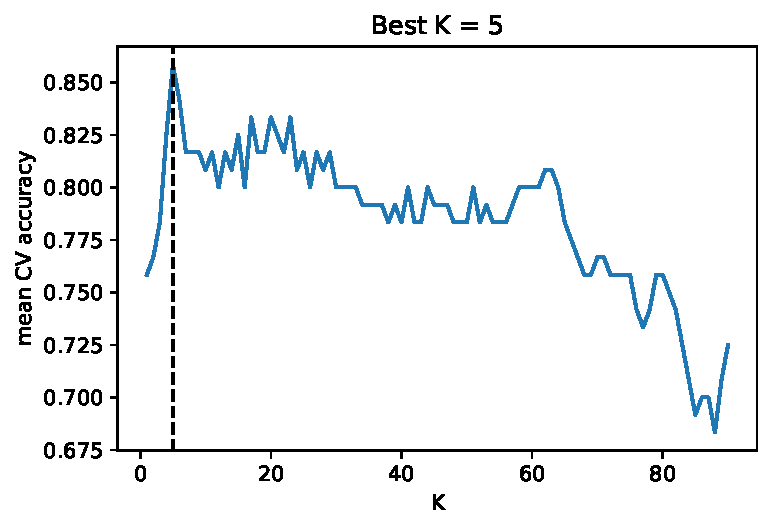
\includegraphics[keepaspectratio]{contents/2/knn_files/figure-pdf/cell-16-output-2.pdf}}

\subsection{Decision Boundary}\label{decision-boundary}

We can visualize the decision boundary using
\texttt{DecisionBoundaryDisplay}.

\begin{Shaded}
\begin{Highlighting}[]
\ImportTok{from}\NormalTok{ sklearn.inspection }\ImportTok{import}\NormalTok{ DecisionBoundaryDisplay}

\NormalTok{pipe.set\_params(}
\NormalTok{    kneighborsclassifier\_\_n\_neighbors}\OperatorTok{=}\NormalTok{grid.best\_params\_[}
        \StringTok{"kneighborsclassifier\_\_n\_neighbors"}
\NormalTok{    ]}
\NormalTok{)}
\NormalTok{pipe.fit(X\_train, y\_train)}

\NormalTok{disp }\OperatorTok{=}\NormalTok{ DecisionBoundaryDisplay.from\_estimator(}
\NormalTok{    pipe,}
\NormalTok{    X\_train,}
\NormalTok{    response\_method}\OperatorTok{=}\StringTok{"predict"}\NormalTok{,}
\NormalTok{    plot\_method}\OperatorTok{=}\StringTok{"pcolormesh"}\NormalTok{,}
\NormalTok{    xlabel}\OperatorTok{=}\NormalTok{iris.feature\_names[}\DecValTok{0}\NormalTok{],}
\NormalTok{    ylabel}\OperatorTok{=}\NormalTok{iris.feature\_names[}\DecValTok{1}\NormalTok{],}
\NormalTok{    alpha}\OperatorTok{=}\FloatTok{0.5}\NormalTok{,}
\NormalTok{)}

\NormalTok{disp.ax\_.scatter(X\_test[:, }\DecValTok{0}\NormalTok{], X\_test[:, }\DecValTok{1}\NormalTok{], c}\OperatorTok{=}\NormalTok{y\_test, marker}\OperatorTok{=}\StringTok{"x"}\NormalTok{, label}\OperatorTok{=}\StringTok{"test"}\NormalTok{)}
\NormalTok{disp.ax\_.scatter(X\_train[:, }\DecValTok{0}\NormalTok{], X\_train[:, }\DecValTok{1}\NormalTok{], c}\OperatorTok{=}\NormalTok{y\_train, alpha}\OperatorTok{=}\FloatTok{0.3}\NormalTok{, label}\OperatorTok{=}\StringTok{"train"}\NormalTok{)}
\NormalTok{plt.title(}\StringTok{"KNN Decision Boundary"}\NormalTok{)}\OperatorTok{;}
\end{Highlighting}
\end{Shaded}

\pandocbounded{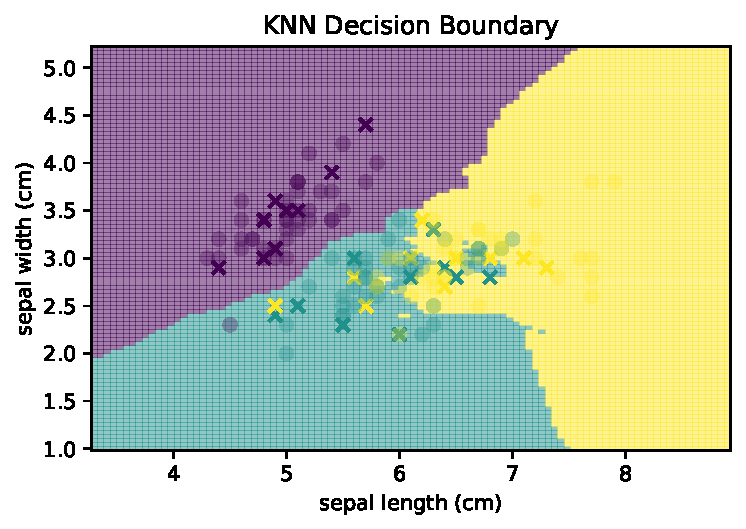
\includegraphics[keepaspectratio]{contents/2/knn_files/figure-pdf/cell-17-output-1.pdf}}

\chapter{Kernel Smoothing}\label{kernel-smoothing}

Kernel smoothing is a family of nonparametric methods for estimating
smooth functions from data. Like KNN, it is based on local information:
nearby observations should have more influence than distant
observations.

The difference is that KNN uses a hard neighbor set, while kernel
methods usually use smoothly decaying weights.

\begin{tcolorbox}[enhanced jigsaw, arc=.35mm, bottomrule=.15mm, bottomtitle=1mm, breakable, colback=white, colbacktitle=quarto-callout-note-color!10!white, colframe=quarto-callout-note-color-frame, coltitle=black, left=2mm, leftrule=.75mm, opacityback=0, opacitybacktitle=0.6, rightrule=.15mm, title=\textcolor{quarto-callout-note-color}{\faInfo}\hspace{0.5em}{Note}, titlerule=0mm, toprule=.15mm, toptitle=1mm]

This chapter focuses on \textbf{kernel smoothing}, including kernel
density estimation and kernel regression. It does not cover kernel
machines such as support vector machines or kernel ridge regression.
These methods also use kernel functions, but their modeling goals are
different.

\end{tcolorbox}

Unlike many methods discussed earlier in this book, classical kernel
smoothing is not fully integrated into the standard \texttt{sklearn}
estimator framework. Although \texttt{sklearn} provides some related
tools, such as \texttt{KernelDensity}, it does not provide a standard
estimator for classical kernel regression.

In this chapter, we will use \texttt{KernelReg} from
\texttt{statsmodels} to fit kernel regression models. For readers
interested in the implementation details, we also include an optional
section on building a custom regressor using the \texttt{sklearn} API
and implementing the estimator from scratch. The goal is not only to
understand how kernel regression works, but also to become familiar with
practical tools from \texttt{statsmodels} and the basic structure of
custom \texttt{sklearn} estimators.

\section{From KNN to Kernel Weights}\label{from-knn-to-kernel-weights}

KNN regression predicts by averaging the \(K\) nearest responses. This
gives equal weight to all \(K\) nearest neighbors and zero weight to
every other observation. In other words, KNN is a weighted average with
hard weights:

\[
\hat f_{\text{KNN}}(x_0)
=
\sum_{i=1}^n w_i(x_0)y_i,
\]

where

\[
w_i(x_0)
=
\begin{cases}
1/K, & i\in N_K(x_0),\\
0, & i\notin N_K(x_0).
\end{cases}
\]

Kernel smoothing keeps the same local-averaging idea but changes the
weights. Instead of deciding whether a point is inside or outside the
neighbor set, it assigns a smooth weight based on distance:

\[
w_i(x_0)
\propto
K\left(\frac{x_0-x_i}{h}\right).
\]

Here \(K(\cdot)\) is the kernel function and \(h>0\) is the bandwidth.

A kernel function converts distance into weight. It gives larger values
to points near zero and smaller values to points far from zero. For
density estimation, we usually require

\[
K(u)\ge 0,
\qquad
\int_{-\infty}^{\infty}K(u)\,du=1.
\]

The scaled kernel is

\[
K_h(x,x_i)
=
\frac{1}{h}
K\left(\frac{x-x_i}{h}\right).
\]

The bandwidth \(h\) controls the distance scale. A small \(h\) makes the
kernel narrow and local; a large \(h\) makes it wide and smooth.

Common choices include:

\begin{itemize}
\tightlist
\item
  Gaussian kernel: \(K(u)=\frac{1}{\sqrt{2\pi}}\exp\qty(-u^2/2)\).
\item
  Uniform kernel: \(K(u)=I(\abs{u}\le 1/2)\).
\item
  Tricube kernel: \(K(u)=(1-\abs{u}^3)^3I(\abs{u}\le 1)\).
\end{itemize}

KNN fits are often discontinuous because the neighbor set can change
abruptly as \(x_0\) moves. Kernel smoothers, especially with smooth
kernels such as the Gaussian kernel, usually produce smooth fitted
curves.

In practice, the exact kernel shape is usually less important than the
bandwidth. The bandwidth controls the main bias--variance tradeoff.

\section{Kernel Density Estimation}\label{kernel-density-estimation}

Suppose a random variable has an unknown density function \(f(x)\).
Given a sample \(\qty{x_1,\ldots,x_n}\), we would like to estimate this
density from the observed data.

Kernel density estimation (KDE) is a nonparametric method for doing so.
The kernel density estimator is

\[
\hat f(x)
=
\frac{1}{n}
\sum_{i=1}^n
K_h(x,x_i).
\]

Equivalently,

\[
\hat f(x)
=
\frac{1}{nh}
\sum_{i=1}^n
K\left(\frac{x-x_i}{h}\right).
\]

The interpretation is simple: place a small smooth bump at every
observation, add the bumps together, and divide by \(n\).

The kernel function determines the shape of each bump, while the
bandwidth \(h\) controls its width. As we will see, the bandwidth is
usually the most important tuning parameter in kernel density
estimation.

We demonstrate the idea with the following example. We use two normal
distributions to generate a simple dataset. The dataset is \texttt{x},
and its histogram is displayed below.

\begin{Shaded}
\begin{Highlighting}[]
\ImportTok{import}\NormalTok{ numpy }\ImportTok{as}\NormalTok{ np}
\ImportTok{import}\NormalTok{ matplotlib.pyplot }\ImportTok{as}\NormalTok{ plt}

\NormalTok{rng }\OperatorTok{=}\NormalTok{ np.random.default\_rng(}\DecValTok{1}\NormalTok{)}

\NormalTok{n1 }\OperatorTok{=}\NormalTok{ rng.normal(loc}\OperatorTok{={-}}\FloatTok{1.0}\NormalTok{, scale}\OperatorTok{=}\FloatTok{0.55}\NormalTok{, size}\OperatorTok{=}\DecValTok{150}\NormalTok{)}
\NormalTok{n2 }\OperatorTok{=}\NormalTok{ rng.normal(loc}\OperatorTok{=}\FloatTok{1.2}\NormalTok{, scale}\OperatorTok{=}\FloatTok{0.35}\NormalTok{, size}\OperatorTok{=}\DecValTok{100}\NormalTok{)}
\NormalTok{x }\OperatorTok{=}\NormalTok{ np.concatenate([n1, n2])}

\NormalTok{plt.hist(x, bins}\OperatorTok{=}\DecValTok{20}\NormalTok{, density}\OperatorTok{=}\VariableTok{True}\NormalTok{, alpha}\OperatorTok{=}\FloatTok{0.35}\NormalTok{, edgecolor}\OperatorTok{=}\StringTok{"black"}\NormalTok{)}
\NormalTok{plt.xlabel(}\StringTok{"x"}\NormalTok{)}
\NormalTok{plt.ylabel(}\StringTok{"density"}\NormalTok{)}\OperatorTok{;}
\end{Highlighting}
\end{Shaded}

\pandocbounded{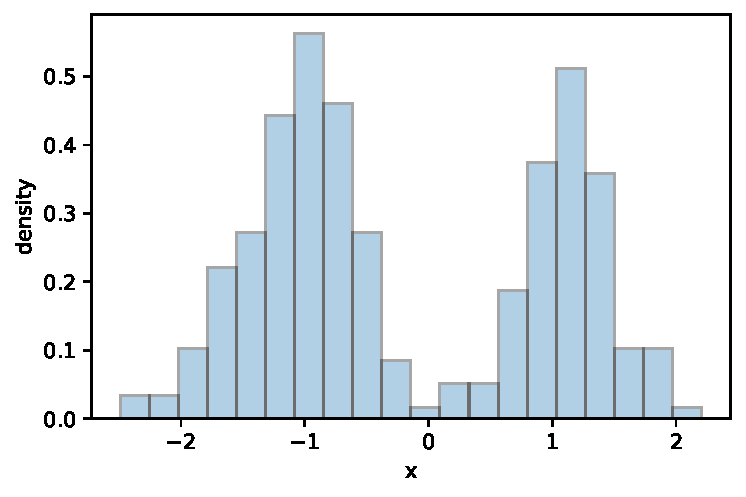
\includegraphics[keepaspectratio]{contents/2/kernel_files/figure-pdf/cell-2-output-1.pdf}}

\subsection{Uniform Kernel and
Histograms}\label{uniform-kernel-and-histograms}

A histogram estimates density by counting observations inside fixed
bins. Kernel density estimation generalizes this idea by replacing fixed
bins with a moving window.

The uniform kernel estimator is itself a valid kernel density estimator.
Histograms and uniform KDE are closely related: histograms use fixed
bins, while uniform KDE centers a window at each evaluation point and
moves that window continuously across the domain.

Using the uniform kernel

\[
K(u)=
\begin{cases}
1,&\abs{u}\leq1/2,\\
0,&\text{otherwise,}
\end{cases}
\]

the kernel density estimator becomes

\[
\hat f(x)
=
\frac{
\#\{x_i:x_i\in[x-h/2,x+h/2]\}
}{nh}.
\]

This can be viewed as a moving histogram. Instead of counting
observations in fixed bins, we center a window of width \(h\) at the
evaluation point \(x\) and count the observations that fall inside the
window. The value \texttt{h=0.35} is chosen solely for illustration. In
practice, selecting an appropriate bandwidth is an important problem and
often requires careful study.

\begin{Shaded}
\begin{Highlighting}[]
\NormalTok{x\_grid }\OperatorTok{=}\NormalTok{ np.linspace(x.}\BuiltInTok{min}\NormalTok{() }\OperatorTok{{-}} \DecValTok{1}\NormalTok{, x.}\BuiltInTok{max}\NormalTok{() }\OperatorTok{+} \DecValTok{1}\NormalTok{, }\DecValTok{500}\NormalTok{)}
\NormalTok{h }\OperatorTok{=} \FloatTok{0.35}

\NormalTok{counts }\OperatorTok{=}\NormalTok{ [np.mean((x }\OperatorTok{\textgreater{}=}\NormalTok{ x0 }\OperatorTok{{-}}\NormalTok{ h }\OperatorTok{/} \DecValTok{2}\NormalTok{) }\OperatorTok{\&}\NormalTok{ (x }\OperatorTok{\textless{}=}\NormalTok{ x0 }\OperatorTok{+}\NormalTok{ h }\OperatorTok{/} \DecValTok{2}\NormalTok{)) }\OperatorTok{/}\NormalTok{ h }\ControlFlowTok{for}\NormalTok{ x0 }\KeywordTok{in}\NormalTok{ x\_grid]}

\NormalTok{plt.hist(x, bins}\OperatorTok{=}\DecValTok{20}\NormalTok{, density}\OperatorTok{=}\VariableTok{True}\NormalTok{, alpha}\OperatorTok{=}\FloatTok{0.35}\NormalTok{, edgecolor}\OperatorTok{=}\StringTok{"black"}\NormalTok{)}
\NormalTok{plt.plot(x\_grid, counts, color}\OperatorTok{=}\StringTok{"C1"}\NormalTok{, linewidth}\OperatorTok{=}\DecValTok{2}\NormalTok{, label}\OperatorTok{=}\StringTok{"uniform kernel"}\NormalTok{)}
\NormalTok{plt.xlabel(}\StringTok{"x"}\NormalTok{)}
\NormalTok{plt.ylabel(}\StringTok{"density"}\NormalTok{)}
\NormalTok{plt.title(}\StringTok{"Uniform Kernel Density Estimate"}\NormalTok{)}
\NormalTok{plt.legend()}\OperatorTok{;}
\end{Highlighting}
\end{Shaded}

\pandocbounded{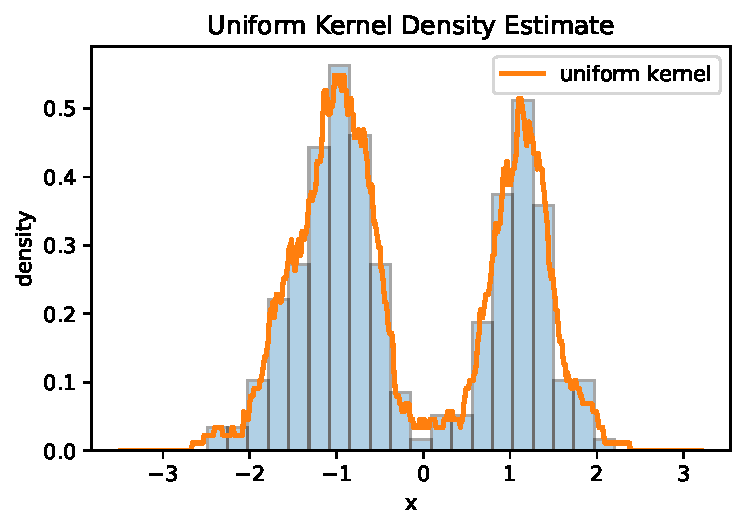
\includegraphics[keepaspectratio]{contents/2/kernel_files/figure-pdf/cell-3-output-1.pdf}}

\subsection{Gaussian KDE}\label{gaussian-kde}

The uniform kernel gives equal weight to all observations inside the
window and zero weight to observations outside. A Gaussian kernel uses a
smoother weighting scheme in which nearby observations receive more
weight than distant observations.

The Gaussian kernel is

\[
K(u)=\frac{1}{\sqrt{2\pi}}
e^{-u^2/2}.
\]

Substituting this kernel into the kernel density estimator gives

\[
\hat f(x)=\frac{1}{nh\sqrt{2\pi}}
\sum_{i=1}^{n}
\exp\qty(-\frac12\qty(\frac{x-x_i}{h})^2).
\]

This estimator can be interpreted as placing a small Gaussian density
centered at each observation and then summing the contributions from all
observations. The bandwidth \(h\) controls the width of these Gaussian
curves.

In practice, kernel density estimation is usually performed using
software rather than by evaluating the formula directly.
\texttt{KernelDensity} from \texttt{sklearn.neighbors} provides an
implementation of KDE with several kernel choices, including the
Gaussian kernel.

\protect\phantomsection\label{annotated-cell-144}%
\begin{Shaded}
\begin{Highlighting}[]
\ImportTok{from}\NormalTok{ sklearn.neighbors }\ImportTok{import}\NormalTok{ KernelDensity}

\NormalTok{kde }\OperatorTok{=}\NormalTok{ KernelDensity(kernel}\OperatorTok{=}\StringTok{"gaussian"}\NormalTok{, bandwidth}\OperatorTok{=}\FloatTok{0.25} \OperatorTok{*}\NormalTok{ x.std())}
\NormalTok{kde.fit(x.reshape(}\OperatorTok{{-}}\DecValTok{1}\NormalTok{, }\DecValTok{1}\NormalTok{)) }\CommentTok{\# \textless{}1\textgreater{}}

\NormalTok{log\_density }\OperatorTok{=}\NormalTok{ kde.score\_samples(x\_grid.reshape(}\OperatorTok{{-}}\DecValTok{1}\NormalTok{, }\DecValTok{1}\NormalTok{))}
\NormalTok{density }\OperatorTok{=}\NormalTok{ np.exp(log\_density)}
\end{Highlighting}
\end{Shaded}

\begin{description}
\tightlist
\item[5CB6E08D-list-annote-1]
As with most \texttt{sklearn} estimators, \texttt{KernelDensity} expects
a 2D predictor matrix. Therefore the 1D array \texttt{x} is reshaped to
an \(n\times 1\) matrix before fitting the model.
\end{description}

The method \texttt{.score\_samples()} returns the logarithm of the
estimated density rather than the density itself. This is done for
numerical stability. Applying \texttt{np.exp()} converts the values back
to the density scale.

\begin{Shaded}
\begin{Highlighting}[]
\NormalTok{plt.hist(x, bins}\OperatorTok{=}\DecValTok{20}\NormalTok{, density}\OperatorTok{=}\VariableTok{True}\NormalTok{, alpha}\OperatorTok{=}\FloatTok{0.35}\NormalTok{, edgecolor}\OperatorTok{=}\StringTok{"black"}\NormalTok{)}
\NormalTok{plt.plot(x\_grid, density, color}\OperatorTok{=}\StringTok{"C1"}\NormalTok{, linewidth}\OperatorTok{=}\DecValTok{2}\NormalTok{, label}\OperatorTok{=}\StringTok{"Gaussian KDE"}\NormalTok{)}
\NormalTok{plt.xlabel(}\StringTok{"x"}\NormalTok{)}
\NormalTok{plt.ylabel(}\StringTok{"density"}\NormalTok{)}
\NormalTok{plt.title(}\StringTok{"Gaussian Kernel Density Estimate"}\NormalTok{)}
\NormalTok{plt.legend()}\OperatorTok{;}
\end{Highlighting}
\end{Shaded}

\pandocbounded{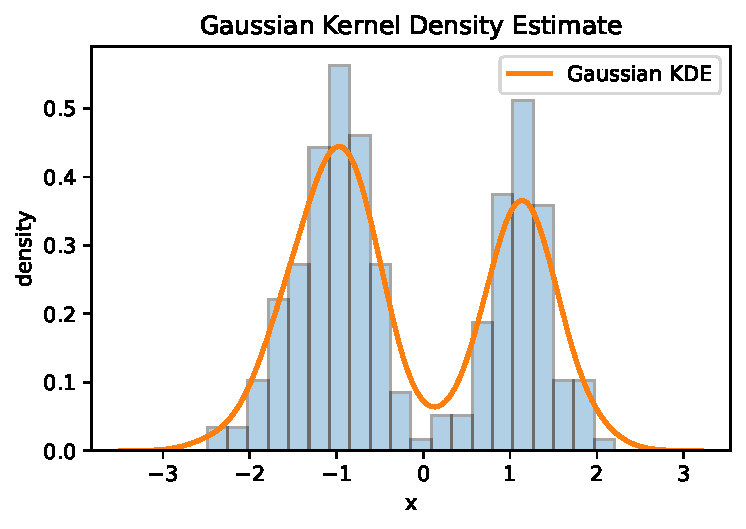
\includegraphics[keepaspectratio]{contents/2/kernel_files/figure-pdf/cell-5-output-1.pdf}}

\subsection{Bias and Variance of KDE}\label{bias-and-variance-of-kde}

To better understand why kernel density estimation works, let us examine
the bias and variance of the estimator.

Assume \(x_1,\ldots,x_n\) are independent samples from a density \(f\).
The estimator is

\[
\hat f(x)
=
\frac{1}{n}
\sum_{i=1}^n
\frac{1}{h}
K\left(\frac{x-x_i}{h}\right).
\]

\begin{theorem}[Bias of KDE]\protect\hypertarget{thm-}{}\label{thm-}

Assume K is a symmetric kernel with finite second moment and f is twice
continuously differentiable. \[
\operatorname{Bias}\qty[\hat f(x)]=O(h^2).
\]

Click for proof.

Since the observations are i.i.d., each term in the sum has the same
expectation. Therefore

\[
\begin{aligned}
\Exp[\hat f(x)]
&=\frac1n
\sum_{i=1}^n
\Exp\!\left[
\frac1h
K\!\left(\frac{x-x_i}{h}\right)
\right]\\
&=\Exp\left[
\frac{1}{h}K\left(\frac{x-X}{h}\right)
\right] \\
&=
\int
\frac{1}{h}
K\left(\frac{x-t}{h}\right)
f(t)\dd t.
\end{aligned}
\]

Let

\[
u=\frac{x-t}{h},
\qquad
t=x-hu.
\]

Then \(\dd t=-h\dd u\). Therefore

\[
\begin{split}
\Exp[\hat f(x)]
=&\int\frac1h K\qty(\frac{x-t}{h})f(t)\dd t\\
=&\int\frac1h K\qty(u)f(x-hu)(-h\dd u)\\
=&\int K(u)f(x-hu)\dd u.
\end{split}
\]

Consider the Taylor series expansion \[
f(x-hu)=f(x)-huf'(x)+\frac12h^2u^2f''(x)+O(h^3u^3).
\]

We have \[
\begin{split}
\Exp[\hat f(x)]&=\int K(u)\qty[f(x)-huf'(x)+\frac12h^2u^2f''(x)+O(h^3u^3)]\dd u\\
&=\int K(u)f(x)\dd u-\int K(u)huf'(x)\dd u+\int\frac12K(u) h^2u^2f''(x)\dd u+\int K(u)O(h^3\abs{u}^3)\dd u\\
&=f(x)\int K(u)\dd u-f'(x)h\int uK(u)\dd u+\frac12h^2f''(x)\int u^2K(u)\dd u+O(h^3)\int \abs{u}^3K(u)\dd u.
\end{split}
\]

Because a kernel function satisfies \[
\int K(u)\dd u=1,
\] and a symmetric kernel satisfies \[
\int uK(u)\dd u = 0,
\] and \[
\int \abs{u}^3K(u)\dd u<\infty,
\]

we have

\[
\begin{split}
\Exp[\hat f(x)]-f(x)
&=\frac12h^2f''(x)\int u^2K(u)\dd u+O(h^3)\\
&=O(h^2).
\end{split}
\]

Then after plugged in, we have \[
\mathrm{Bias}=\Exp[\hat f(x)]-f(x)=O(h^2).
\]

\end{theorem}

\begin{tcolorbox}[enhanced jigsaw, arc=.35mm, bottomrule=.15mm, bottomtitle=1mm, breakable, colback=white, colbacktitle=quarto-callout-note-color!10!white, colframe=quarto-callout-note-color-frame, coltitle=black, left=2mm, leftrule=.75mm, opacityback=0, opacitybacktitle=0.6, rightrule=.15mm, title=\textcolor{quarto-callout-note-color}{\faInfo}\hspace{0.5em}{Note}, titlerule=0mm, toprule=.15mm, toptitle=1mm]

The expectation of the KDE is a weighted average of nearby values of the
true density. Therefore KDE estimates a smoothed version of the
underlying density. In fact, the expectation can be viewed as a
convolution of the density and a rescaled kernel.

\end{tcolorbox}

\begin{theorem}[Variance of KDE]\protect\hypertarget{thm-}{}\label{thm-}

Assume \(f\) is continuous at \(x\), and \(K\) satisfies
\(\int K^2(u)\,du<\infty\). \[
\Var[\hat f(x)]
=
O\!\left(
\frac1{nh}
\right).
\]

Click for proof.

Since the observations are independent,

\[
\Var[\hat f(x)]
=
\frac1{n^2}
\sum_{i=1}^n
\Var\left[
\frac1h K\left(\frac{x-x_i}{h}\right)
\right].
\]

All terms have the same variance, so

\[
\Var[\hat f(x)]
=
\frac1n
\Var\left[
\frac1h K\left(\frac{x-X}{h}\right)
\right].
\]

Using the definition of variance,

\[
\Var\left[
\frac1h K\left(\frac{x-X}{h}\right)
\right]
=
\Exp\left[
\frac1{h^2}K^2\left(\frac{x-X}{h}\right)
\right]
-
\left\{
\Exp\left[
\frac1h K\left(\frac{x-X}{h}\right)
\right]
\right\}^2.
\]

For the first term,

\[
\begin{aligned}
\Exp\left[
\frac1{h^2}K^2\left(\frac{x-X}{h}\right)
\right]
&=
\int
\frac1{h^2}
K^2\left(\frac{x-t}{h}\right)
f(t)\dd t \\
&=
\frac1h
\int
K^2(u)f(x-hu)\dd u.
\end{aligned}
\]

When \(h\) is small and \(f\) is assumed smooth near \(x\),

\[
f(x-hu)=f(x)+O(h\abs{u}).
\]

Therefore

\[
\Exp\left[
\frac1{h^2}K^2\left(\frac{x-X}{h}\right)
\right]
=
\frac{f(x)}{h}
\int K^2(u)\dd u
+\frac{O(h)}h\int \abs{u}K^2(u)\dd u.
\]

Since \(f(x)\) and \(\int K^2(u)\dd u\) are constants, then \[
\Exp\left[
\frac1{h^2}K^2\left(\frac{x-X}{h}\right)
\right]
=
O\left(\frac1h\right).
\]

The second term is

\[
\left\{
\Exp\left[
\frac1h K\left(\frac{x-X}{h}\right)
\right]
\right\}^2=\qty{\Exp\qty[\hat f(x)]}^2.
\]

From the bias calculation,

\[
\Exp[\hat f(x)]
=
f(x)+O(h^2),
\]

so this squared term is

\[
\begin{split}
\left(f(x)+O(h^2)\right)^2
=&f(x)^2+2f(x)O(h^2)+O(h^4)\\
=&f(x)^2+O(h^2)\\
=O(1).
\end{split}
\]

Hence

\[
\Var\left[
\frac1h K\left(\frac{x-X}{h}\right)
\right]
=O\qty(\frac1h)-O(1)=O\qty(\frac1h).
\]

Finally,

\[
\Var[\hat f(x)]
=
\frac1nO\qty(\frac1h)=O(\frac1{nh}).
\]

\end{theorem}

Therefore the pointwise mean squared error of KDE estimator satisfies

\[
\operatorname{MSE}\qty[\hat f(x)]=\qty(\operatorname{Bias}\qty[\hat f(x)])^2+\Var\qty[\hat f(x)]
=
O(h^4)
+
O\!\left(
\frac1{nh}
\right).
\]

Reducing the bandwidth decreases the magnitude of the bias but increases
the variance. Bandwidth selection therefore involves a bias-variance
tradeoff.

\begin{tcolorbox}[enhanced jigsaw, arc=.35mm, bottomrule=.15mm, bottomtitle=1mm, breakable, colback=white, colbacktitle=quarto-callout-note-color!10!white, colframe=quarto-callout-note-color-frame, coltitle=black, left=2mm, leftrule=.75mm, opacityback=0, opacitybacktitle=0.6, rightrule=.15mm, title=\textcolor{quarto-callout-note-color}{\faInfo}\hspace{0.5em}{Note}, titlerule=0mm, toprule=.15mm, toptitle=1mm]

Balancing the two dominant terms, \(h^4 \asymp \frac1{nh}\), which
implies \(h \asymp n^{-1/5}\). This explains why many rule-of-thumb
bandwidth formulas involve the factor \$ n\^{}\{-1/5\} \$.

\end{tcolorbox}

\begin{tcolorbox}[enhanced jigsaw, arc=.35mm, bottomrule=.15mm, bottomtitle=1mm, breakable, colback=white, colbacktitle=quarto-callout-note-color!10!white, colframe=quarto-callout-note-color-frame, coltitle=black, left=2mm, leftrule=.75mm, opacityback=0, opacitybacktitle=0.6, rightrule=.15mm, title=\textcolor{quarto-callout-note-color}{\faInfo}\hspace{0.5em}{The Practical Impact of Bandwidth}, titlerule=0mm, toprule=.15mm, toptitle=1mm]

The bandwidth controls the smoothness of the density estimate and has a
much larger effect on the result than the choice of kernel.

\begin{itemize}
\tightlist
\item
  Small Bandwidth (Low Bias / High Variance): The estimate follows the
  observed data very closely and can capture fine-scale features.
  However, it is often sensitive to random sampling variation and may
  produce spurious peaks that do not correspond to genuine structure in
  the underlying distribution.
\item
  Large Bandwidth (High Bias / Low Variance): The estimate is smoother
  and less sensitive to random fluctuations. However, excessive
  smoothing can obscure important characteristics of the distribution,
  such as skewness, heavy tails, or multiple modes.
\end{itemize}

As a result, the same dataset can produce substantially different
density estimates when different bandwidth values are used.

For most practical applications, selecting an appropriate bandwidth is
far more important than selecting a particular kernel function.
Consequently, bandwidth selection is the central tuning problem in
kernel density estimation.

\end{tcolorbox}

\subsection{Rule-of-Thumb Bandwidth Selection for
KDE}\label{rule-of-thumb-bandwidth-selection-for-kde}

Numerous bandwidth selection methods have been proposed.

The asymptotic bias-variance analysis above implies that an optimal
bandwidth should decrease roughly at the rate \(h = O(n^{-1/5})\).

For a Gaussian kernel, a widely used rule-of-thumb bandwidth is

\[
h=1.06\,\hat\sigma\, n^{-1/5}.
\]

This formula is derived under the assumption that the underlying density
is approximately Gaussian and is commonly known as Silverman's rule of
thumb.

The following Python code implements this rule.

\begin{Shaded}
\begin{Highlighting}[]
\NormalTok{h }\OperatorTok{=} \FloatTok{1.06} \OperatorTok{*}\NormalTok{ np.std(x, ddof}\OperatorTok{=}\DecValTok{1}\NormalTok{) }\OperatorTok{*} \BuiltInTok{len}\NormalTok{(x) }\OperatorTok{**}\NormalTok{ (}\OperatorTok{{-}}\DecValTok{1} \OperatorTok{/} \DecValTok{5}\NormalTok{)}
\end{Highlighting}
\end{Shaded}

Rule-of-thumb formulas are computationally inexpensive and often provide
reasonable starting values. However, they rely on simplifying
assumptions and may perform poorly when the underlying density differs
substantially from those assumptions.

\subsection{Bandwidth Selection by Visual
Inspection}\label{bandwidth-selection-by-visual-inspection}

Bandwidth selection for KDE can be performed using cross-validation,
plug-in methods, or other data-driven procedures.

However, KDE is often used for exploratory visualization. In such
settings, practitioners frequently inspect several nearby bandwidth
values visually to assess the stability of the estimated density.

\begin{Shaded}
\begin{Highlighting}[]
\NormalTok{bandwidths }\OperatorTok{=}\NormalTok{ [}\FloatTok{0.1}\NormalTok{, }\FloatTok{0.3}\NormalTok{, }\FloatTok{0.6}\NormalTok{]}

\NormalTok{plt.hist(x, bins}\OperatorTok{=}\DecValTok{20}\NormalTok{, density}\OperatorTok{=}\VariableTok{True}\NormalTok{, alpha}\OperatorTok{=}\FloatTok{0.25}\NormalTok{, edgecolor}\OperatorTok{=}\StringTok{"black"}\NormalTok{)}

\ControlFlowTok{for}\NormalTok{ bw }\KeywordTok{in}\NormalTok{ bandwidths:}
\NormalTok{    kde }\OperatorTok{=}\NormalTok{ KernelDensity(kernel}\OperatorTok{=}\StringTok{"gaussian"}\NormalTok{, bandwidth}\OperatorTok{=}\NormalTok{bw)}
\NormalTok{    kde.fit(x.reshape(}\OperatorTok{{-}}\DecValTok{1}\NormalTok{, }\DecValTok{1}\NormalTok{))}
\NormalTok{    density }\OperatorTok{=}\NormalTok{ np.exp(kde.score\_samples(x\_grid.reshape(}\OperatorTok{{-}}\DecValTok{1}\NormalTok{, }\DecValTok{1}\NormalTok{)))}
\NormalTok{    plt.plot(x\_grid, density, linewidth}\OperatorTok{=}\DecValTok{2}\NormalTok{, label}\OperatorTok{=}\SpecialStringTok{f"h=}\SpecialCharTok{\{}\NormalTok{bw}\SpecialCharTok{\}}\SpecialStringTok{"}\NormalTok{)}

\NormalTok{plt.xlabel(}\StringTok{"x"}\NormalTok{)}
\NormalTok{plt.ylabel(}\StringTok{"density"}\NormalTok{)}
\NormalTok{plt.title(}\StringTok{"Choosing Bandwidth by Visual Inspection"}\NormalTok{)}
\NormalTok{plt.legend()}\OperatorTok{;}
\end{Highlighting}
\end{Shaded}

\pandocbounded{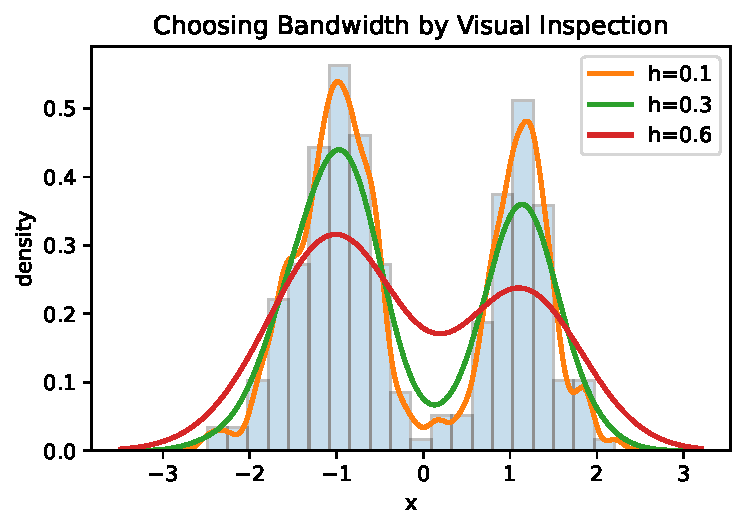
\includegraphics[keepaspectratio]{contents/2/kernel_files/figure-pdf/cell-8-output-1.pdf}}

The figure compares KDE estimates with several bandwidth values.

\begin{itemize}
\tightlist
\item
  With \texttt{h=0.1}, the density estimate contains many small peaks
  and valleys. These fluctuations are likely caused by sampling noise
  rather than genuine features of the underlying distribution.
\item
  With \texttt{h=0.6}, the estimate is much smoother, but some local
  features have disappeared.
\item
  With \texttt{h=0.3}, the estimate preserves the main shape of the
  distribution while avoiding excessive noise.
\end{itemize}

A common visual strategy is to choose the smallest bandwidth that
removes obvious noise while preserving important features such as peaks,
valleys, skewness, or multiple modes.

\section{Kernel Regression}\label{kernel-regression}

Kernel regression estimates

\[
f(x)=\Exp[Y\mid X=x].
\]

The most common kernel regression estimator is the Nadaraya-Watson
estimator.

\begin{definition}[Nadaraya-Watson
estimator]\protect\hypertarget{def-nadaraya-watson}{}\label{def-nadaraya-watson}

Given training data \((x_i,y_i)\), the Nadaraya-Watson estimator is

\[
\hat f(x)
=
\frac{
\sum_{i=1}^n K_h(x,x_i)y_i
}{
\sum_{i=1}^n K_h(x,x_i)
}.
\]

\end{definition}

This is a weighted average of the responses. The weights are

\[
w_i(x)
=
\frac{
K_h(x,x_i)
}{
\sum_{j=1}^n K_h(x,x_j)
}.
\]

Thus

\[
\hat f(x)
=
\sum_{i=1}^n w_i(x)y_i,
\qquad
\sum_{i=1}^n w_i(x)=1.
\]

For the Gaussian kernel,

\[
K_h(x,x_i)
=
\frac{1}{h\sqrt{2\pi}}
\exp\left\{
-\frac{(x-x_i)^2}{2h^2}
\right\}.
\]

\subsection{Comparing KNN and Kernel
Regression}\label{comparing-knn-and-kernel-regression}

The following example compares a KNN regression curve with a Gaussian
kernel regression curve on the same data.

We first generate a one-feature dataset and a grid for plotting
predictions. The data are generated from \[
y=2\sin(x)+\varepsilon, 
\] so the true regression function is \(f(x)=2\sin(x)\). We will use
this function as a reference when evaluating the fitted models.

\begin{Shaded}
\begin{Highlighting}[]
\NormalTok{rng }\OperatorTok{=}\NormalTok{ np.random.default\_rng(}\DecValTok{1}\NormalTok{)}

\NormalTok{X }\OperatorTok{=}\NormalTok{ rng.uniform(}\DecValTok{0}\NormalTok{, }\DecValTok{2} \OperatorTok{*}\NormalTok{ np.pi, size}\OperatorTok{=}\DecValTok{40}\NormalTok{)}
\NormalTok{y }\OperatorTok{=} \DecValTok{2} \OperatorTok{*}\NormalTok{ np.sin(X) }\OperatorTok{+}\NormalTok{ rng.normal(size}\OperatorTok{=}\BuiltInTok{len}\NormalTok{(X))}
\NormalTok{X\_grid }\OperatorTok{=}\NormalTok{ np.linspace(}\DecValTok{0}\NormalTok{, }\DecValTok{2} \OperatorTok{*}\NormalTok{ np.pi, }\DecValTok{500}\NormalTok{)}
\end{Highlighting}
\end{Shaded}

For comparison we fit a KNN regressor with \texttt{n\_neighbors=10}.
Since the purpose is to show the idea, for simplicity we do not split
train-test or tune \(K\).

\begin{Shaded}
\begin{Highlighting}[]
\ImportTok{from}\NormalTok{ sklearn.neighbors }\ImportTok{import}\NormalTok{ KNeighborsRegressor}

\NormalTok{knn }\OperatorTok{=}\NormalTok{ KNeighborsRegressor(n\_neighbors}\OperatorTok{=}\DecValTok{10}\NormalTok{)}
\NormalTok{knn.fit(X.reshape(}\OperatorTok{{-}}\DecValTok{1}\NormalTok{, }\DecValTok{1}\NormalTok{), y)}
\NormalTok{y\_knn }\OperatorTok{=}\NormalTok{ knn.predict(X\_grid.reshape(}\OperatorTok{{-}}\DecValTok{1}\NormalTok{, }\DecValTok{1}\NormalTok{))}
\end{Highlighting}
\end{Shaded}

Now we fit a Nadaraya-Watson estimator using \texttt{KernelReg} from
\texttt{statsmodels}.

\begin{Shaded}
\begin{Highlighting}[]
\ImportTok{from}\NormalTok{ statsmodels.nonparametric.kernel\_regression }\ImportTok{import}\NormalTok{ KernelReg}

\NormalTok{h }\OperatorTok{=} \FloatTok{0.25}
\NormalTok{kr }\OperatorTok{=}\NormalTok{ KernelReg(endog}\OperatorTok{=}\NormalTok{y, exog}\OperatorTok{=}\NormalTok{X, reg\_type}\OperatorTok{=}\StringTok{"lc"}\NormalTok{, bw}\OperatorTok{=}\NormalTok{[h], var\_type}\OperatorTok{=}\StringTok{"c"}\NormalTok{)}
\NormalTok{y\_kernel, \_ }\OperatorTok{=}\NormalTok{ kr.fit(X\_grid)}
\end{Highlighting}
\end{Shaded}

The bandwidth is chosen to be 0.25. This is only a simple starting
value; bandwidth tuning is discussed later.

\begin{Shaded}
\begin{Highlighting}[]
\NormalTok{fig, axs }\OperatorTok{=}\NormalTok{ plt.subplots(}\DecValTok{1}\NormalTok{, }\DecValTok{2}\NormalTok{, figsize}\OperatorTok{=}\NormalTok{(}\DecValTok{12}\NormalTok{, }\DecValTok{4}\NormalTok{), sharey}\OperatorTok{=}\VariableTok{True}\NormalTok{)}

\NormalTok{axs[}\DecValTok{0}\NormalTok{].scatter(X, y, s}\OperatorTok{=}\DecValTok{35}\NormalTok{, facecolors}\OperatorTok{=}\StringTok{"none"}\NormalTok{, edgecolors}\OperatorTok{=}\StringTok{"black"}\NormalTok{)}
\NormalTok{axs[}\DecValTok{0}\NormalTok{].plot(X\_grid, }\DecValTok{2} \OperatorTok{*}\NormalTok{ np.sin(X\_grid), color}\OperatorTok{=}\StringTok{"C0"}\NormalTok{, label}\OperatorTok{=}\StringTok{"true function"}\NormalTok{)}
\NormalTok{axs[}\DecValTok{0}\NormalTok{].plot(X\_grid, y\_knn, color}\OperatorTok{=}\StringTok{"C1"}\NormalTok{, label}\OperatorTok{=}\StringTok{"KNN"}\NormalTok{)}
\NormalTok{axs[}\DecValTok{0}\NormalTok{].set\_title(}\StringTok{"KNN Regression"}\NormalTok{)}

\NormalTok{axs[}\DecValTok{1}\NormalTok{].scatter(X, y, s}\OperatorTok{=}\DecValTok{35}\NormalTok{, facecolors}\OperatorTok{=}\StringTok{"none"}\NormalTok{, edgecolors}\OperatorTok{=}\StringTok{"black"}\NormalTok{)}
\NormalTok{axs[}\DecValTok{1}\NormalTok{].plot(X\_grid, }\DecValTok{2} \OperatorTok{*}\NormalTok{ np.sin(X\_grid), color}\OperatorTok{=}\StringTok{"C0"}\NormalTok{, label}\OperatorTok{=}\StringTok{"true function"}\NormalTok{)}
\NormalTok{axs[}\DecValTok{1}\NormalTok{].plot(X\_grid, y\_kernel, color}\OperatorTok{=}\StringTok{"C2"}\NormalTok{, label}\OperatorTok{=}\StringTok{"Nadaraya{-}Watson"}\NormalTok{)}
\NormalTok{axs[}\DecValTok{1}\NormalTok{].set\_title(}\StringTok{"Nadaraya{-}Watson estimator"}\NormalTok{)}

\ControlFlowTok{for}\NormalTok{ ax }\KeywordTok{in}\NormalTok{ axs:}
\NormalTok{    ax.set\_xlabel(}\StringTok{"x"}\NormalTok{)}
\NormalTok{    ax.legend()}

\NormalTok{axs[}\DecValTok{0}\NormalTok{].set\_ylabel(}\StringTok{"y"}\NormalTok{)}\OperatorTok{;}
\end{Highlighting}
\end{Shaded}

\pandocbounded{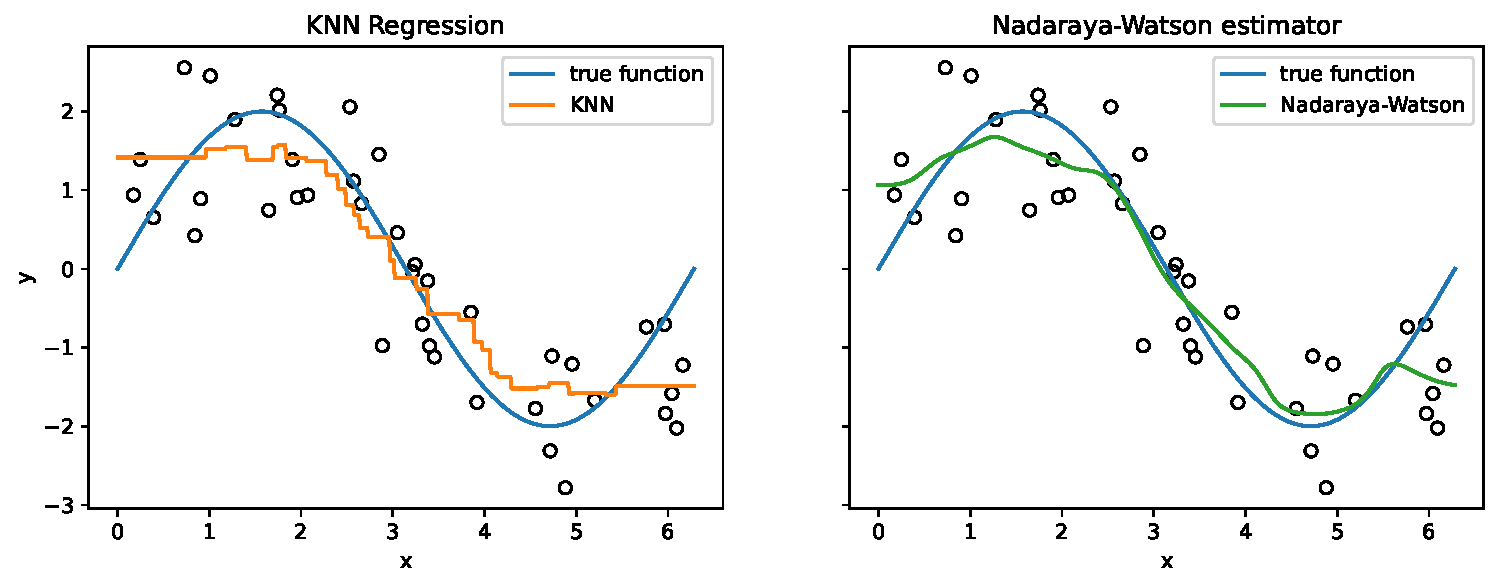
\includegraphics[keepaspectratio]{contents/2/kernel_files/figure-pdf/cell-12-output-1.pdf}}

The KNN fit is piecewise constant because the prediction is the average
of a fixed set of nearest neighbors. As the target point moves, the
neighbor set may suddenly change, causing abrupt jumps in the fitted
curve.

The Nadaraya-Watson estimator fit changes smoothly because every
observation contributes to the prediction. The weights vary continuously
with distance, producing a smooth estimate of the regression function.

\subsection{\texorpdfstring{Understanding
\texttt{KernelReg}}{Understanding KernelReg}}\label{understanding-kernelreg}

The API of \texttt{KernelReg} from \texttt{statsmodels} differs
substantially from the APIs used by most \texttt{sklearn} estimators, so
we briefly explain the most important arguments and methods. More
details can be found in the
\href{https://www.statsmodels.org/devel/generated/statsmodels.nonparametric.kernel_regression.KernelReg.html}{official
document}.

\subsubsection{\texorpdfstring{Different
\texttt{fit}}{Different fit}}\label{different-fit}

Unlike most \texttt{sklearn} estimators, \texttt{KernelReg} does not
have a separate training step. The training data are supplied when the
object is created, and the \texttt{fit()} method is used to evaluate the
fitted regression function at new points. In other words,
\texttt{y\_hat,\ \_\ =\ kr.fit(X)} performs prediction at the input
locations \texttt{X}.

\begin{itemize}
\tightlist
\item
  The first returned value is the estimated conditional mean.
\item
  The second returned value contains estimated marginal effects.
\item
  In this chapter, we only use the fitted values, so the marginal
  effects are discarded by assigning them to \texttt{\_}.
\end{itemize}

\subsubsection{\texorpdfstring{\texttt{endog} and
\texttt{exog}}{endog and exog}}\label{endog-and-exog}

The model is initialized using \texttt{endog=y} and \texttt{exog=X}.

\begin{itemize}
\tightlist
\item
  \texttt{endog}: endogenous variable
\item
  \texttt{exog}: exogenous variable
\item
  These terms come from econometrics. In a statistical learning context,
  you can simply think of them as \texttt{endog=y} and \texttt{exog=X}.
\end{itemize}

\subsubsection{Regressor type}\label{regressor-type}

\texttt{reg\_type="lc"} specifies the regression estimator.

\begin{itemize}
\tightlist
\item
  \texttt{"lc"} stands for local constant regression, which corresponds
  to the Nadaraya-Watson estimator introduced earlier.
\item
  \texttt{"ll"} stands for local linear regression.
\item
  The default is \texttt{"ll"}.
\end{itemize}

\subsubsection{Bandwidth}\label{bandwidth}

\texttt{bw} specifies the bandwidth.

\begin{itemize}
\tightlist
\item
  It can be supplied directly as a numeric value, as in this example.
\item
  Explicit bandwidth values should be provided as a list. This design
  allows a separate bandwidth for each predictor. For one-dimensional
  regression, the list contains only one element.
\item
  Alternatively, setting \texttt{bw="cv\_ls"} instructs
  \texttt{KernelReg} to select the bandwidth automatically using
  least-squares cross-validation. This will be discussed later.
\end{itemize}

\subsubsection{Variable type}\label{variable-type}

\texttt{var\_type} specifies the type of each predictor variable:

\begin{itemize}
\tightlist
\item
  \texttt{"c"}: continuous
\item
  \texttt{"u"}: unordered discrete
\item
  \texttt{"o"}: ordered discrete
\end{itemize}

\texttt{var\_type="c"} indicates that the predictor is continuous. For
multiple predictors, \texttt{var\_type} should contain one character for
each predictor. For example, \texttt{"ccc"} indicates three continuous
predictors.

\subsection{Local Averaging at One Target
Point}\label{local-averaging-at-one-target-point}

The key idea of kernel regression is local weighted averaging. In this
section we use the previous example to visualize this behavior: at a
target point \(x_0\), observations closer to \(x_0\) receive larger
kernel weights.

If we just want to predict the value at \(x_0\) we can directly apply
\texttt{KernelReg}. However it doesn't return all the weights. Therefore
here we manually implement the algorithm in this section. Note that
\texttt{y\_kernel} is the one fitted with \texttt{KernelReg} from
previous codes.

Recall that the Nadaraya-Watson estimate at \(x_0\) is the weighted
average

\[
\hat f(x_0)
=\sum_{i=1}^nw_i(x_0)y_i,\quad\text{ where }\quad w_i(x_0)=\frac{K_h(x_0,x_i)}{\sum_{j=1}^nK_h(x_0,x_j)}.
\]

with a Gaussian kernel,

\[
K_h(x_0,x_i)
=
\frac{1}{h\sqrt{2\pi}}
\exp\left\{
-\frac{(x_0-x_i)^2}{2h^2}
\right\}.
\]

Because the Nadaraya-Watson estimator normalizes the weights, the
constant \(1/(h\sqrt{2\pi})\) cancels out. Therefore, for regression
weights, it is enough to use

\[
\mathrm{raw_weights}=\exp\left\{
-\frac{(x_0-x_i)^2}{2h^2}
\right\}.
\]

We first compute the kernel weights for the target point \(x_0=3\) with
\(h=0.25\).

\begin{Shaded}
\begin{Highlighting}[]
\NormalTok{x0 }\OperatorTok{=} \FloatTok{3.0}
\NormalTok{h }\OperatorTok{=} \FloatTok{0.25}

\NormalTok{raw\_weights }\OperatorTok{=}\NormalTok{ np.exp(}\OperatorTok{{-}}\FloatTok{0.5} \OperatorTok{*}\NormalTok{ ((x0 }\OperatorTok{{-}}\NormalTok{ X) }\OperatorTok{/}\NormalTok{ h) }\OperatorTok{**} \DecValTok{2}\NormalTok{)}
\NormalTok{fhat\_x0 }\OperatorTok{=}\NormalTok{ np.}\BuiltInTok{sum}\NormalTok{(raw\_weights }\OperatorTok{*}\NormalTok{ y) }\OperatorTok{/}\NormalTok{ np.}\BuiltInTok{sum}\NormalTok{(raw\_weights)}
\end{Highlighting}
\end{Shaded}

We then use the weights to determine the size of each plotted point, so
that larger circles correspond to larger kernel weights. The factor 1200
is chosen only for visualization.

\begin{Shaded}
\begin{Highlighting}[]
\NormalTok{point\_sizes }\OperatorTok{=} \DecValTok{1200} \OperatorTok{*}\NormalTok{ raw\_weights }\OperatorTok{/}\NormalTok{ raw\_weights.}\BuiltInTok{sum}\NormalTok{()}
\end{Highlighting}
\end{Shaded}

We can now plot the data together with the fitted curve, using the
assigned point sizes to represent the kernel weights.

\protect\phantomsection\label{annotated-cell-154}%
\begin{Shaded}
\begin{Highlighting}[]
\ImportTok{import}\NormalTok{ matplotlib.pyplot }\ImportTok{as}\NormalTok{ plt}

\NormalTok{plt.scatter(X, y, s}\OperatorTok{=}\NormalTok{point\_sizes, facecolors}\OperatorTok{=}\StringTok{"none"}\NormalTok{, edgecolors}\OperatorTok{=}\StringTok{"black"}\NormalTok{)}
\NormalTok{plt.plot(X\_grid, }\DecValTok{2} \OperatorTok{*}\NormalTok{ np.sin(X\_grid), color}\OperatorTok{=}\StringTok{"C0"}\NormalTok{, label}\OperatorTok{=}\StringTok{"true function"}\NormalTok{)}
\NormalTok{plt.plot(X\_grid, y\_kernel, color}\OperatorTok{=}\StringTok{"C1"}\NormalTok{, label}\OperatorTok{=}\StringTok{"kernel regression"}\NormalTok{)}

\NormalTok{plt.scatter([x0], [fhat\_x0], color}\OperatorTok{=}\StringTok{"red"}\NormalTok{, s}\OperatorTok{=}\DecValTok{80}\NormalTok{, zorder}\OperatorTok{=}\DecValTok{3}\NormalTok{, label}\OperatorTok{=}\VerbatimStringTok{r"}\DecValTok{$}\ErrorTok{\textbackslash{}}\VerbatimStringTok{hat f}\KeywordTok{(}\VerbatimStringTok{x\_0}\KeywordTok{)}\DecValTok{$}\VerbatimStringTok{"}\NormalTok{) }\CommentTok{\# \textless{}1\textgreater{}}
\NormalTok{plt.axvline(x0, color}\OperatorTok{=}\StringTok{"black"}\NormalTok{, linestyle}\OperatorTok{=}\StringTok{"{-}{-}"}\NormalTok{, alpha}\OperatorTok{=}\FloatTok{0.5}\NormalTok{)}

\NormalTok{plt.xlabel(}\StringTok{"x"}\NormalTok{)}
\NormalTok{plt.ylabel(}\StringTok{"y"}\NormalTok{)}
\NormalTok{plt.title(}\StringTok{"Kernel Weights Around a Target Point"}\NormalTok{)}
\NormalTok{plt.legend()}\OperatorTok{;}
\end{Highlighting}
\end{Shaded}

\begin{description}
\tightlist
\item[5CB6E08D-list-annote-1]
We specifically plot the estimated point.
\end{description}

\pandocbounded{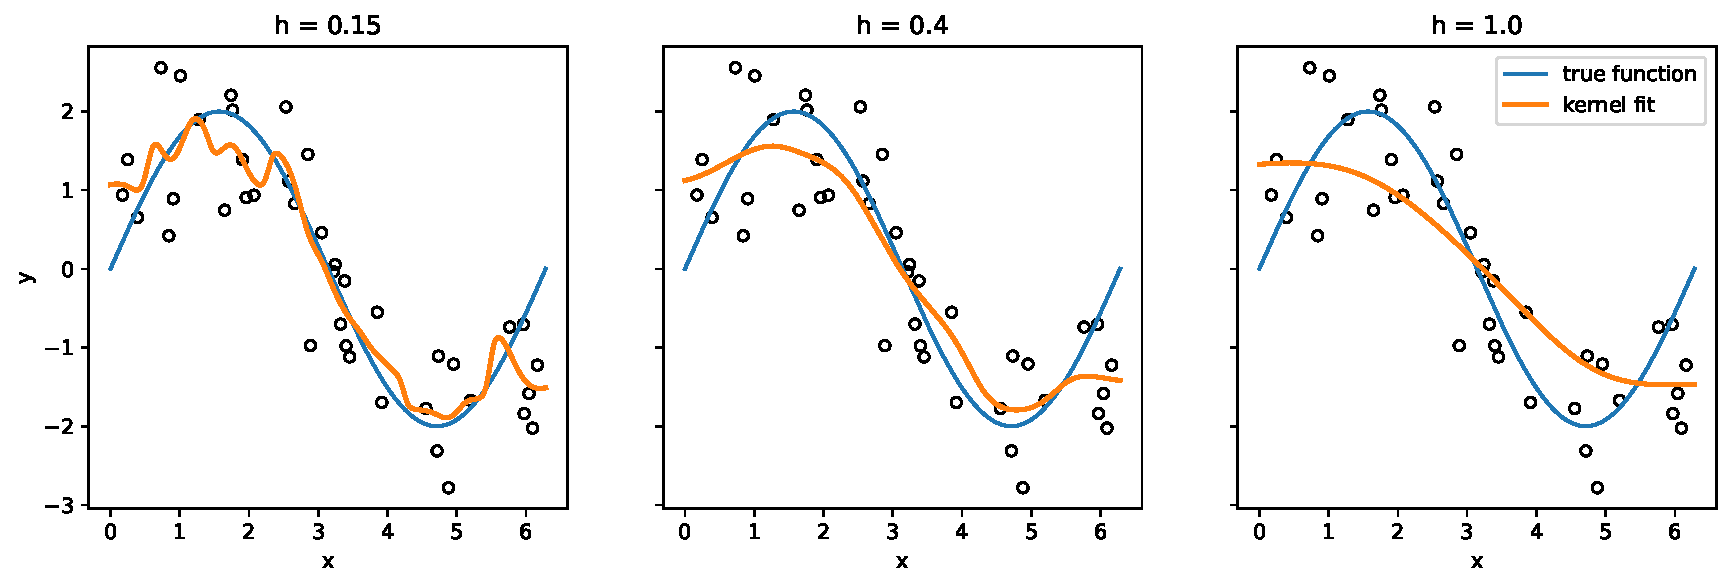
\includegraphics[keepaspectratio]{contents/2/kernel_files/figure-pdf/cell-15-output-1.pdf}}

The circle sizes are proportional to the kernel weights. Points near
\(x_0\) receive larger weights and therefore have a greater influence on
the local average. Points farther away receive smaller weights and
contribute less to the estimate.

We may apply the same code to different target points to show the
effects of different weights.

\protect\phantomsection\label{annotated-cell-155}%
\begin{Shaded}
\begin{Highlighting}[]
\ImportTok{import}\NormalTok{ matplotlib.pyplot }\ImportTok{as}\NormalTok{ plt}

\NormalTok{x0\_values }\OperatorTok{=}\NormalTok{ [}\FloatTok{1.0}\NormalTok{, }\FloatTok{2.5}\NormalTok{, }\FloatTok{4.0}\NormalTok{, }\FloatTok{5.5}\NormalTok{]}
\NormalTok{h }\OperatorTok{=} \FloatTok{0.25}

\NormalTok{fig, axes }\OperatorTok{=}\NormalTok{ plt.subplots(}\DecValTok{2}\NormalTok{, }\DecValTok{2}\NormalTok{, figsize}\OperatorTok{=}\NormalTok{(}\DecValTok{10}\NormalTok{, }\DecValTok{8}\NormalTok{))}
\NormalTok{axes }\OperatorTok{=}\NormalTok{ axes.ravel() }\CommentTok{\# \textless{}1\textgreater{}}

\ControlFlowTok{for}\NormalTok{ ax, x0 }\KeywordTok{in} \BuiltInTok{zip}\NormalTok{(axes, x0\_values):}
\NormalTok{    raw\_weights }\OperatorTok{=}\NormalTok{ np.exp(}\OperatorTok{{-}}\FloatTok{0.5} \OperatorTok{*}\NormalTok{ ((x0 }\OperatorTok{{-}}\NormalTok{ X) }\OperatorTok{/}\NormalTok{ h) }\OperatorTok{**} \DecValTok{2}\NormalTok{)}
\NormalTok{    point\_sizes }\OperatorTok{=} \DecValTok{1200} \OperatorTok{*}\NormalTok{ raw\_weights }\OperatorTok{/}\NormalTok{ raw\_weights.}\BuiltInTok{sum}\NormalTok{()}
\NormalTok{    fhat\_x0 }\OperatorTok{=}\NormalTok{ np.}\BuiltInTok{sum}\NormalTok{(raw\_weights }\OperatorTok{*}\NormalTok{ y) }\OperatorTok{/}\NormalTok{ np.}\BuiltInTok{sum}\NormalTok{(raw\_weights)}

\NormalTok{    ax.scatter(X, y, s}\OperatorTok{=}\NormalTok{point\_sizes, facecolors}\OperatorTok{=}\StringTok{"none"}\NormalTok{, edgecolors}\OperatorTok{=}\StringTok{"black"}\NormalTok{)}

\NormalTok{    ax.plot(X\_grid, }\DecValTok{2} \OperatorTok{*}\NormalTok{ np.sin(X\_grid), color}\OperatorTok{=}\StringTok{"C0"}\NormalTok{, label}\OperatorTok{=}\StringTok{"true function"}\NormalTok{)}
\NormalTok{    ax.plot(X\_grid, y\_kernel, color}\OperatorTok{=}\StringTok{"C1"}\NormalTok{, label}\OperatorTok{=}\StringTok{"kernel regression"}\NormalTok{)}

\NormalTok{    ax.scatter([x0], [fhat\_x0], color}\OperatorTok{=}\StringTok{"red"}\NormalTok{, s}\OperatorTok{=}\DecValTok{80}\NormalTok{, zorder}\OperatorTok{=}\DecValTok{3}\NormalTok{, label}\OperatorTok{=}\VerbatimStringTok{r"}\DecValTok{$}\ErrorTok{\textbackslash{}}\VerbatimStringTok{hat f}\KeywordTok{(}\VerbatimStringTok{x\_0}\KeywordTok{)}\DecValTok{$}\VerbatimStringTok{"}\NormalTok{)}
\NormalTok{    ax.axvline(x0, color}\OperatorTok{=}\StringTok{"black"}\NormalTok{, linestyle}\OperatorTok{=}\StringTok{"{-}{-}"}\NormalTok{, alpha}\OperatorTok{=}\FloatTok{0.5}\NormalTok{)}

\NormalTok{    ax.set\_title(}\SpecialStringTok{f"$x\_0=}\SpecialCharTok{\{}\NormalTok{x0}\SpecialCharTok{\}}\SpecialStringTok{$"}\NormalTok{)}
\NormalTok{    ax.set\_xlabel(}\StringTok{"x"}\NormalTok{)}
\NormalTok{    ax.set\_ylabel(}\StringTok{"y"}\NormalTok{)}

\NormalTok{axes[}\DecValTok{0}\NormalTok{].legend()}
\NormalTok{plt.tight\_layout()}\OperatorTok{;}
\end{Highlighting}
\end{Shaded}

\begin{description}
\tightlist
\item[5CB6E08D-list-annote-1]
The original \texttt{axes} object is a 2-by-2 array, so we would need to
use \texttt{axes{[}0,\ 0{]}} to access the upper-left plot. After
flattening it with \texttt{ravel()}, we can use \texttt{axes{[}0{]}},
\texttt{axes{[}1{]}}, and so on. This makes the loop simpler because we
do not need to track the row and column indices explicitly.
\end{description}

\pandocbounded{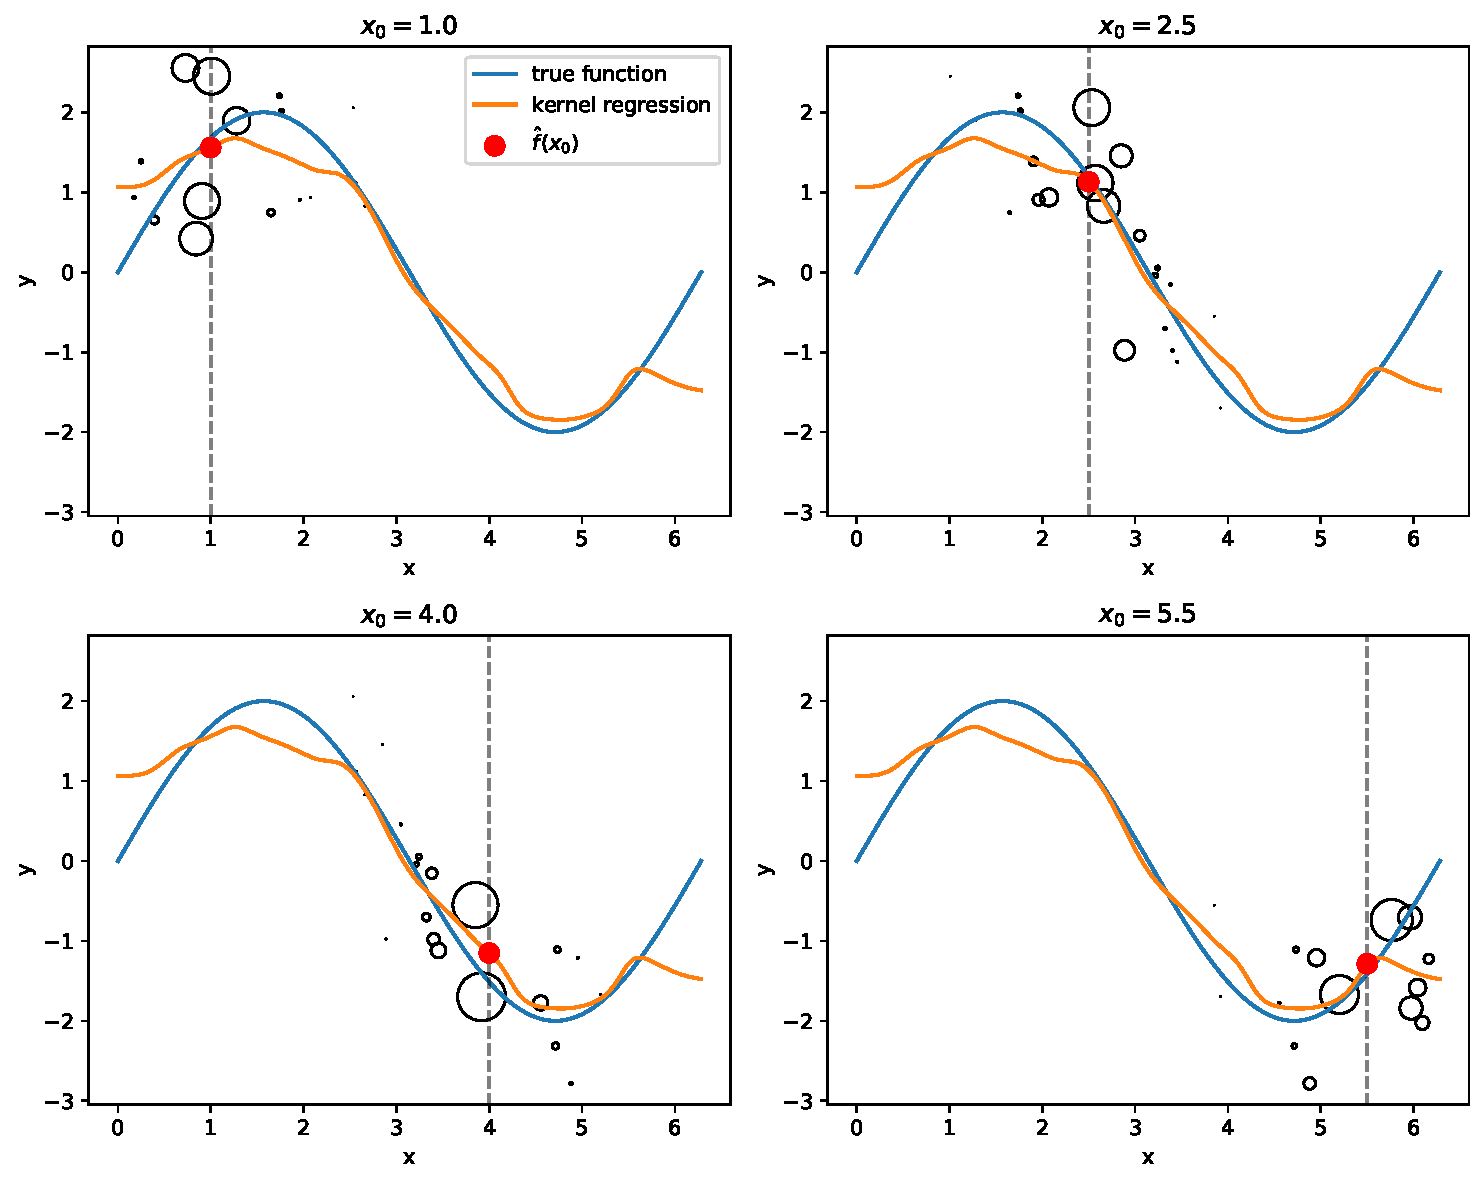
\includegraphics[keepaspectratio]{contents/2/kernel_files/figure-pdf/cell-16-output-1.pdf}}

\subsection{Effect of Bandwidth in Kernel
Regression}\label{effect-of-bandwidth-in-kernel-regression}

Bandwidth plays the same role in kernel regression as it does in kernel
density estimation. A small bandwidth gives more weight to nearby
observations and produces a more flexible fit, while a large bandwidth
averages over a wider neighborhood and produces a smoother fit.

Under suitable regularity conditions, it can be shown that kernel
regression exhibits the same bias-variance tradeoff as KDE: decreasing
the bandwidth reduces bias but increases variance, while increasing the
bandwidth has the opposite effect. The exact formulas are more
complicated than in KDE, so we focus on the visual behavior here.

\begin{Shaded}
\begin{Highlighting}[]
\NormalTok{X\_grid }\OperatorTok{=}\NormalTok{ np.linspace(}\DecValTok{0}\NormalTok{, }\DecValTok{2} \OperatorTok{*}\NormalTok{ np.pi, }\DecValTok{500}\NormalTok{)}

\NormalTok{fig, axs }\OperatorTok{=}\NormalTok{ plt.subplots(}\DecValTok{1}\NormalTok{, }\DecValTok{3}\NormalTok{, figsize}\OperatorTok{=}\NormalTok{(}\DecValTok{14}\NormalTok{, }\DecValTok{4}\NormalTok{), sharey}\OperatorTok{=}\VariableTok{True}\NormalTok{)}

\ControlFlowTok{for}\NormalTok{ ax, bw }\KeywordTok{in} \BuiltInTok{zip}\NormalTok{(axs, [}\FloatTok{0.15}\NormalTok{, }\FloatTok{0.4}\NormalTok{, }\FloatTok{1.0}\NormalTok{]):}
\NormalTok{    kr }\OperatorTok{=}\NormalTok{ KernelReg(endog}\OperatorTok{=}\NormalTok{y, exog}\OperatorTok{=}\NormalTok{X, bw}\OperatorTok{=}\NormalTok{[bw], reg\_type}\OperatorTok{=}\StringTok{\textquotesingle{}lc\textquotesingle{}}\NormalTok{, var\_type}\OperatorTok{=}\StringTok{\textquotesingle{}c\textquotesingle{}}\NormalTok{)}
\NormalTok{    y\_hat, \_ }\OperatorTok{=}\NormalTok{ kr.fit(X\_grid)}

\NormalTok{    ax.scatter(X, y, s}\OperatorTok{=}\DecValTok{25}\NormalTok{, facecolors}\OperatorTok{=}\StringTok{"none"}\NormalTok{, edgecolors}\OperatorTok{=}\StringTok{"black"}\NormalTok{)}
\NormalTok{    ax.plot(X\_grid, }\DecValTok{2} \OperatorTok{*}\NormalTok{ np.sin(X\_grid), color}\OperatorTok{=}\StringTok{"C0"}\NormalTok{, label}\OperatorTok{=}\StringTok{"true function"}\NormalTok{)}
\NormalTok{    ax.plot(X\_grid, y\_hat, color}\OperatorTok{=}\StringTok{"C1"}\NormalTok{, linewidth}\OperatorTok{=}\DecValTok{2}\NormalTok{, label}\OperatorTok{=}\StringTok{"kernel fit"}\NormalTok{)}
\NormalTok{    ax.set\_title(}\SpecialStringTok{f"h = }\SpecialCharTok{\{}\NormalTok{bw}\SpecialCharTok{\}}\SpecialStringTok{"}\NormalTok{)}
\NormalTok{    ax.set\_xlabel(}\StringTok{"x"}\NormalTok{)}

\NormalTok{axs[}\DecValTok{0}\NormalTok{].set\_ylabel(}\StringTok{"y"}\NormalTok{)}
\NormalTok{axs[}\OperatorTok{{-}}\DecValTok{1}\NormalTok{].legend()}\OperatorTok{;}
\end{Highlighting}
\end{Shaded}

\pandocbounded{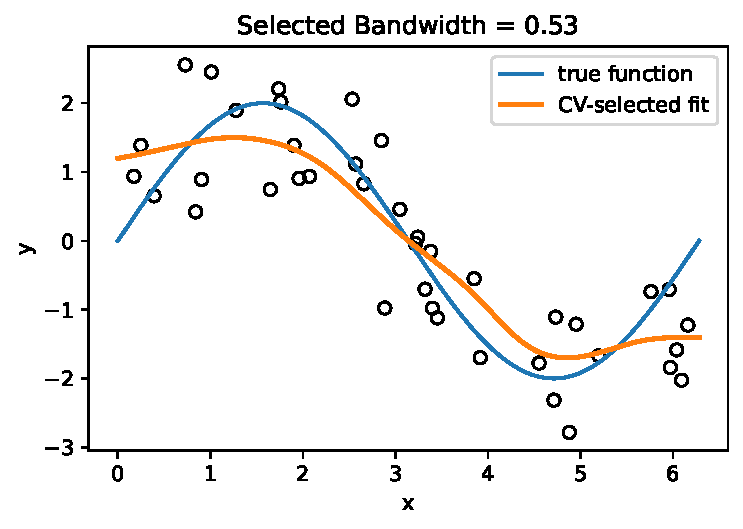
\includegraphics[keepaspectratio]{contents/2/kernel_files/figure-pdf/cell-17-output-1.pdf}}

The figure illustrates the effect of bandwidth on the fitted curve.

\begin{itemize}
\tightlist
\item
  When the bandwidth is small (\(h=0.15\)), the fit follows local
  fluctuations closely. This reduces smoothing bias but increases
  variability.
\item
  With a moderate bandwidth (\(h=0.4\)), the fit captures the overall
  trend while remaining reasonably smooth.
\item
  When the bandwidth is large (\(h=1.0\)), the fit becomes overly smooth
  and may miss important features of the underlying function.
\end{itemize}

As the bandwidth increases, variance decreases but bias increases.
Choosing an appropriate bandwidth therefore requires balancing these two
sources of error.

\begin{tcolorbox}[enhanced jigsaw, arc=.35mm, bottomrule=.15mm, bottomtitle=1mm, breakable, colback=white, colbacktitle=quarto-callout-note-color!10!white, colframe=quarto-callout-note-color-frame, coltitle=black, left=2mm, leftrule=.75mm, opacityback=0, opacitybacktitle=0.6, rightrule=.15mm, title=\textcolor{quarto-callout-note-color}{\faInfo}\hspace{0.5em}{Kernel Regression MSE}, titlerule=0mm, toprule=.15mm, toptitle=1mm]

For one-dimensional kernel regression, the asymptotic bias is typically
of order \(O(h^2)\), while the variance is of order
\(O\qty(\frac{1}{nh})\). Consequently, the mean squared error behaves
roughly as \(O(h^4)+O\qty(\frac{1}{nh})\), which mirrors the KDE case.

Therefore, although the exact formulas differ from those in KDE, the
same bias-variance tradeoff leads to bandwidth selection rules of a
similar form.

\end{tcolorbox}

\subsection{Bandwidth Selection by
Cross-Validation}\label{bandwidth-selection-by-cross-validation}

Rule-of-thumb methods are fast and easy to use, but they rely on
assumptions that may not hold in practice. Since kernel regression is
typically used for prediction, cross-validation is often preferred as a
more data-driven approach to bandwidth selection.

\texttt{KernelReg} from \texttt{statsmodels} can automatically select
the bandwidth by cross-validation when \texttt{bw="cv\_ls"} is
specified. In this case, leave-one-out cross-validation is used to
search for the bandwidth that minimizes the prediction error.

The cross-validation procedure is performed automatically when the model
is initialized. The selected bandwidth can then be inspected through the
\texttt{bw} attribute.

\begin{Shaded}
\begin{Highlighting}[]
\ImportTok{from}\NormalTok{ statsmodels.nonparametric.kernel\_regression }\ImportTok{import}\NormalTok{ KernelReg}

\NormalTok{kr }\OperatorTok{=}\NormalTok{ KernelReg(endog}\OperatorTok{=}\NormalTok{y, exog}\OperatorTok{=}\NormalTok{X, var\_type}\OperatorTok{=}\StringTok{"c"}\NormalTok{, reg\_type}\OperatorTok{=}\StringTok{"lc"}\NormalTok{, bw}\OperatorTok{=}\StringTok{"cv\_ls"}\NormalTok{)}
\NormalTok{kr.bw}
\end{Highlighting}
\end{Shaded}

\begin{verbatim}
array([0.53263357])
\end{verbatim}

With the selected bandwidth, we can plot the fitted curve.

\begin{Shaded}
\begin{Highlighting}[]
\NormalTok{y\_best, \_ }\OperatorTok{=}\NormalTok{ kr.fit(X\_grid)}

\NormalTok{plt.scatter(X, y, s}\OperatorTok{=}\DecValTok{35}\NormalTok{, facecolors}\OperatorTok{=}\StringTok{"none"}\NormalTok{, edgecolors}\OperatorTok{=}\StringTok{"black"}\NormalTok{)}
\NormalTok{plt.plot(X\_grid, }\DecValTok{2} \OperatorTok{*}\NormalTok{ np.sin(X\_grid), color}\OperatorTok{=}\StringTok{"C0"}\NormalTok{, label}\OperatorTok{=}\StringTok{"true function"}\NormalTok{)}
\NormalTok{plt.plot(X\_grid, y\_best, color}\OperatorTok{=}\StringTok{"C1"}\NormalTok{, linewidth}\OperatorTok{=}\DecValTok{2}\NormalTok{, label}\OperatorTok{=}\StringTok{"CV{-}selected fit"}\NormalTok{)}
\NormalTok{plt.xlabel(}\StringTok{"x"}\NormalTok{)}
\NormalTok{plt.ylabel(}\StringTok{"y"}\NormalTok{)}
\NormalTok{plt.title(}\SpecialStringTok{f"Selected Bandwidth = }\SpecialCharTok{\{}\NormalTok{kr}\SpecialCharTok{.}\NormalTok{bw}\SpecialCharTok{.}\NormalTok{item()}\SpecialCharTok{:.2f\}}\SpecialStringTok{"}\NormalTok{)}
\NormalTok{plt.legend()}\OperatorTok{;}
\end{Highlighting}
\end{Shaded}

\pandocbounded{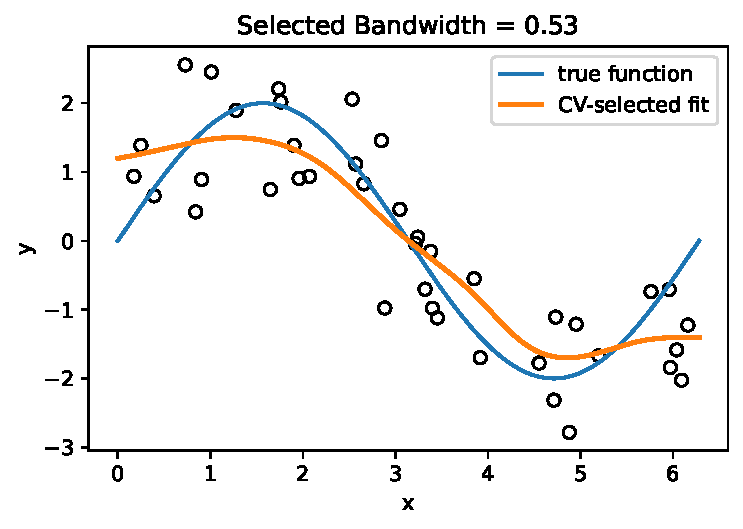
\includegraphics[keepaspectratio]{contents/2/kernel_files/figure-pdf/cell-19-output-1.pdf}}

\section{Extensions}\label{extensions}

The basic Nadaraya-Watson estimator is a local constant estimator. It
can be extended in several directions. Two common extensions are local
linear/polynomial regression and LOWESS.

\subsection{Local Linear Regression}\label{local-linear-regression}

Around each target point \(x_0\), local constant regression fits a
weighted constant. Local linear regression instead fits a weighted line:
\[
\min_{\beta_0,\beta_1}
\sum_{i=1}^n
K_h(x_0,x_i)
\left[
y_i-\beta_0-\beta_1(x_i-x_0)
\right]^2.
\]

The predictors are centered at the target point \(x_0\). As a result,
the fitted intercept directly estimates the regression function at that
location.

\[
\hat f(x_0)=\hat\beta_0.
\]

The \texttt{statsmodels} implementation \texttt{KernelReg} supports both
local constant (Nadaraya-Watson) and local linear kernel regression
through the \texttt{reg\_type} parameter. Use \texttt{reg\_type="lc"}
for local constant regression and \texttt{reg\_type="ll"} for local
linear regression.

\begin{Shaded}
\begin{Highlighting}[]
\ImportTok{from}\NormalTok{ statsmodels.nonparametric.kernel\_regression }\ImportTok{import}\NormalTok{ KernelReg}

\CommentTok{\# Local constant regression}
\NormalTok{kr\_lc }\OperatorTok{=}\NormalTok{ KernelReg(endog}\OperatorTok{=}\NormalTok{y, exog}\OperatorTok{=}\NormalTok{X, var\_type}\OperatorTok{=}\StringTok{"c"}\NormalTok{, reg\_type}\OperatorTok{=}\StringTok{"lc"}\NormalTok{, bw}\OperatorTok{=}\NormalTok{[}\FloatTok{0.4}\NormalTok{])}
\NormalTok{y\_lc, \_ }\OperatorTok{=}\NormalTok{ kr\_lc.fit(X\_grid)}

\CommentTok{\# Local linear regression}
\NormalTok{kr\_ll }\OperatorTok{=}\NormalTok{ KernelReg(endog}\OperatorTok{=}\NormalTok{y, exog}\OperatorTok{=}\NormalTok{X, var\_type}\OperatorTok{=}\StringTok{"c"}\NormalTok{, reg\_type}\OperatorTok{=}\StringTok{"ll"}\NormalTok{, bw}\OperatorTok{=}\NormalTok{[}\FloatTok{0.4}\NormalTok{])}
\NormalTok{y\_ll, \_ }\OperatorTok{=}\NormalTok{ kr\_ll.fit(X\_grid)}
\end{Highlighting}
\end{Shaded}

\begin{Shaded}
\begin{Highlighting}[]
\NormalTok{plt.scatter(X, y, s}\OperatorTok{=}\DecValTok{35}\NormalTok{, facecolors}\OperatorTok{=}\StringTok{"none"}\NormalTok{, edgecolors}\OperatorTok{=}\StringTok{"black"}\NormalTok{)}
\NormalTok{plt.plot(X\_grid, }\DecValTok{2} \OperatorTok{*}\NormalTok{ np.sin(X\_grid), color}\OperatorTok{=}\StringTok{"C0"}\NormalTok{, label}\OperatorTok{=}\StringTok{"true function"}\NormalTok{)}
\NormalTok{plt.plot(X\_grid, y\_lc, color}\OperatorTok{=}\StringTok{"C1"}\NormalTok{, label}\OperatorTok{=}\StringTok{"local constant"}\NormalTok{)}
\NormalTok{plt.plot(X\_grid, y\_ll, color}\OperatorTok{=}\StringTok{"C2"}\NormalTok{, label}\OperatorTok{=}\StringTok{"local linear"}\NormalTok{)}
\NormalTok{plt.xlabel(}\StringTok{"x"}\NormalTok{)}
\NormalTok{plt.ylabel(}\StringTok{"y"}\NormalTok{)}
\NormalTok{plt.title(}\StringTok{"Local Constant versus Local Linear Smoothing"}\NormalTok{)}
\NormalTok{plt.legend()}\OperatorTok{;}
\end{Highlighting}
\end{Shaded}

\pandocbounded{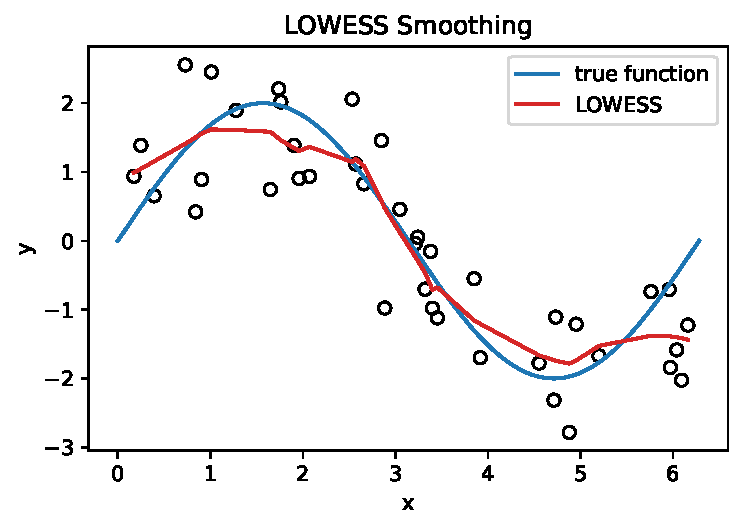
\includegraphics[keepaspectratio]{contents/2/kernel_files/figure-pdf/cell-21-output-1.pdf}}

Local linear regression often improves boundary behavior. Near the
boundary of the data, a local average can be biased because observations
are available on only one side of the target point. A local line can
extrapolate slightly toward the boundary, reducing this additional bias.

\subsection{Local Polynomial
Regression}\label{local-polynomial-regression}

Local linear regression is a special case of local polynomial
regression. At each target point \(x_0\), local polynomial regression
fits

\[
\min_{\beta_0,\ldots,\beta_d}
\sum_{i=1}^n
K_h(x_0,x_i)
\left[
y_i-\beta_0-\sum_{r=1}^d \beta_r(x_i-x_0)^r
\right]^2.
\]

As in local linear regression, centering the predictors at \(x_0\)
ensures that the fitted intercept corresponds to the estimated function
value at the target point.

\[
\hat f(x_0)=\hat\beta_0.
\]

The degree \(d\) controls the local shape:

\begin{itemize}
\tightlist
\item
  \(d=0\): local constant regression (Nadaraya-Watson),
\item
  \(d=1\): local linear regression,
\item
  \(d=2\): local quadratic regression.
\end{itemize}

Higher-degree local polynomials can reduce bias because they capture
more local curvature. However, they also have higher variance and may
become unstable when the bandwidth is small or when only a few
observations receive substantial kernel weight.

Although local polynomial regression can be formulated for any degree
\(d\), the \texttt{KernelReg} implementation in \texttt{statsmodels}
provides only local constant and local linear smoothing. The
\texttt{scikit-learn} library does not currently include local
polynomial regression, although custom implementations can be built
using the standard estimator API. We provide an example of such a custom
implementation at the end of this chapter.

\subsection{LOWESS}\label{lowess}

LOWESS, short for locally weighted scatterplot smoothing, is a local
linear regression method that combines nearest-neighbor neighborhoods
with distance-based weights.

For a target point \(x_0\), LOWESS first selects a neighborhood around
\(x_0\). The neighborhood size is controlled by a span parameter,
usually denoted by \(\alpha\). If the dataset contains \(n\)
observations, the closest \(m=\lceil \alpha n\rceil\) points are used in
the local fit and form the local set \(N(x_0)\).

Let

\[
d(x_0)=\max_{i\in N(x_0)} |x_i-x_0|
\]

be the distance from \(x_0\) to the farthest point in the neighborhood.
LOWESS assigns distance weights using the tricube kernel:

\[
w_i=
\begin{cases}
\left(
1-\left|
\frac{x_i-x_0}{d(x_0)}
\right|^3
\right)^3,
&
|x_i-x_0|<d(x_0),
\\
0,
&
\text{otherwise}.
\end{cases}
\]

At \(x_0\), LOWESS fits a weighted local linear model:

\[
\min_{\beta_0,\beta_1}
\sum_{i=1}^n
w_i
\left[
y_i-\beta_0-\beta_1(x_i-x_0)
\right]^2.
\]

The fitted value is the fitted intercept:

\[
\hat f(x_0)=\hat\beta_0.
\]

Thus, LOWESS can be viewed as a local linear regression method that uses
a nearest-neighbor span instead of a fixed bandwidth. The LOWESS span
can therefore be interpreted as an adaptive bandwidth: it fixes the
number of nearby observations, so the corresponding distance scale
changes with the local data density.

\begin{tcolorbox}[enhanced jigsaw, arc=.35mm, bottomrule=.15mm, bottomtitle=1mm, breakable, colback=white, colbacktitle=quarto-callout-note-color!10!white, colframe=quarto-callout-note-color-frame, coltitle=black, left=2mm, leftrule=.75mm, opacityback=0, opacitybacktitle=0.6, rightrule=.15mm, title=\textcolor{quarto-callout-note-color}{\faInfo}\hspace{0.5em}{LOWESS vs.~kernel regression}, titlerule=0mm, toprule=.15mm, toptitle=1mm]

LOWESS can be viewed as a variant of local linear kernel smoothing. Both
methods fit a weighted local line around each target point.

The main difference is how the neighborhood is defined: local linear
kernel regression uses a fixed bandwidth, whereas LOWESS uses a fixed
fraction of nearby observations, leading to an adaptive bandwidth.
Therefore, LOWESS can be viewed as a local linear smoother with an
adaptive neighborhood size.

\end{tcolorbox}

\subsubsection{LOWESS in Python}\label{lowess-in-python}

In Python, LOWESS is available from
\texttt{statsmodels.nonparametric.smoothers\_lowess}.

\begin{Shaded}
\begin{Highlighting}[]
\ImportTok{from}\NormalTok{ statsmodels.nonparametric.smoothers\_lowess }\ImportTok{import}\NormalTok{ lowess}

\NormalTok{lowess\_result }\OperatorTok{=}\NormalTok{ lowess(endog}\OperatorTok{=}\NormalTok{y, exog}\OperatorTok{=}\NormalTok{X, frac}\OperatorTok{=}\FloatTok{0.25}\NormalTok{, it}\OperatorTok{=}\DecValTok{0}\NormalTok{, return\_sorted}\OperatorTok{=}\VariableTok{True}\NormalTok{)}
\end{Highlighting}
\end{Shaded}

Similar to \texttt{KernelReg}, unlike an estimator object,
\texttt{lowess} directly computes and returns the smoothed values in a
single function call. The argument \texttt{return\_sorted} controls the
format of the output.

\begin{itemize}
\tightlist
\item
  If \texttt{return\_sorted=True}, the output is a two-column NumPy
  array. The first column contains the sorted \texttt{X} values, and the
  second column contains the corresponding fitted values.
\item
  If \texttt{return\_sorted=False}, the output is a one-dimensional
  NumPy array of fitted values in the original order of \texttt{X}.
\item
  If \texttt{xvals} is provided, LOWESS evaluates the fitted smoother at
  those values. In this case, \texttt{return\_sorted} is ignored, and
  the returned array is always one-dimensional.
\item
  \texttt{frac} is the span parameter \(\alpha\). This is the most
  important hyperparameter.
\end{itemize}

\begin{tcolorbox}[enhanced jigsaw, arc=.35mm, bottomrule=.15mm, bottomtitle=1mm, breakable, colback=white, colbacktitle=quarto-callout-note-color!10!white, colframe=quarto-callout-note-color-frame, coltitle=black, left=2mm, leftrule=.75mm, opacityback=0, opacitybacktitle=0.6, rightrule=.15mm, title=\textcolor{quarto-callout-note-color}{\faInfo}\hspace{0.5em}{LOWESS is often used for visualization}, titlerule=0mm, toprule=.15mm, toptitle=1mm]

LOWESS was originally developed as a smoothing method for exploratory
data analysis and visualization. Consequently, many software
implementations emphasize plotting and curve estimation rather than
predictive modeling. This is why the default output uses
\texttt{return\_sorted=True}.

When \texttt{return\_sorted=True}, the returned \(x\)-values are sorted
from low to high, so the fitted curve can be plotted directly.

Like kernel regression, LOWESS can also be used for prediction by
evaluating the fitted smoother at new values through the \texttt{xvals}
argument. However, in practice LOWESS is most commonly used for
visualizing trends and exploring nonlinear relationships rather than for
building predictive models.

\end{tcolorbox}

\subsubsection{Robust LOWESS}\label{robust-lowess}

LOWESS can also perform robustification iterations. After an initial
fit, observations with large residuals receive smaller robustness
weights. The final fit uses both distance-based weights and robustness
weights, so outliers have less influence on the fitted curve.

In \texttt{statsmodels}, the argument \texttt{it} specifies the number
of robustification iterations.

Although \texttt{it} can take any nonnegative integer value, most
applications use either \texttt{it=0} for ordinary LOWESS or
\texttt{it=3} for robust LOWESS. Note that the original LOWESS paper
recommended three robustness iterations, which is why \texttt{it=3}
became the common default in many software packages.

So usually we start from setting \texttt{it=0}, and then try
\texttt{it=3} to see whether it is better.

We fit both ordinary LOWESS (\texttt{it=0}) and robust LOWESS
(\texttt{it=3}) using the same value of \texttt{frac}. Because
\texttt{return\_sorted=True}, each result contains the sorted predictor
values in the first column and the corresponding fitted values in the
second column.

\begin{Shaded}
\begin{Highlighting}[]
\ImportTok{from}\NormalTok{ statsmodels.nonparametric.smoothers\_lowess }\ImportTok{import}\NormalTok{ lowess}

\NormalTok{lowess\_standard }\OperatorTok{=}\NormalTok{ lowess(}
\NormalTok{    endog}\OperatorTok{=}\NormalTok{y, exog}\OperatorTok{=}\NormalTok{X, frac}\OperatorTok{=}\FloatTok{0.25}\NormalTok{, it}\OperatorTok{=}\DecValTok{0}\NormalTok{, return\_sorted}\OperatorTok{=}\VariableTok{True}
\NormalTok{)}

\NormalTok{lowess\_robust }\OperatorTok{=}\NormalTok{ lowess(}
\NormalTok{    endog}\OperatorTok{=}\NormalTok{y, exog}\OperatorTok{=}\NormalTok{X, frac}\OperatorTok{=}\FloatTok{0.25}\NormalTok{, it}\OperatorTok{=}\DecValTok{3}\NormalTok{, return\_sorted}\OperatorTok{=}\VariableTok{True}
\NormalTok{)}
\end{Highlighting}
\end{Shaded}

We then plot the two fitted curves together for comparison.

\begin{Shaded}
\begin{Highlighting}[]
\ImportTok{import}\NormalTok{ matplotlib.pyplot }\ImportTok{as}\NormalTok{ plt}

\NormalTok{plt.scatter(X, y, s}\OperatorTok{=}\DecValTok{35}\NormalTok{, facecolors}\OperatorTok{=}\StringTok{"none"}\NormalTok{, edgecolors}\OperatorTok{=}\StringTok{"black"}\NormalTok{)}
\NormalTok{plt.plot(X\_grid, }\DecValTok{2} \OperatorTok{*}\NormalTok{ np.sin(X\_grid), label}\OperatorTok{=}\StringTok{"true function"}\NormalTok{)}
\NormalTok{plt.plot(}
\NormalTok{    lowess\_standard[:, }\DecValTok{0}\NormalTok{],}
\NormalTok{    lowess\_standard[:, }\DecValTok{1}\NormalTok{],}
\NormalTok{    label}\OperatorTok{=}\StringTok{"LOWESS ($it=0$)"}\NormalTok{,}
\NormalTok{)}
\NormalTok{plt.plot(}
\NormalTok{    lowess\_robust[:, }\DecValTok{0}\NormalTok{],}
\NormalTok{    lowess\_robust[:, }\DecValTok{1}\NormalTok{],}
\NormalTok{    linestyle}\OperatorTok{=}\StringTok{"{-}{-}"}\NormalTok{,}
\NormalTok{    label}\OperatorTok{=}\StringTok{"robust LOWESS ($it=3$)"}\NormalTok{,}
\NormalTok{)}
\NormalTok{plt.xlabel(}\StringTok{"x"}\NormalTok{)}
\NormalTok{plt.ylabel(}\StringTok{"y"}\NormalTok{)}
\NormalTok{plt.title(}\StringTok{"Ordinary versus Robust LOWESS"}\NormalTok{)}
\NormalTok{plt.legend()}
\end{Highlighting}
\end{Shaded}

\pandocbounded{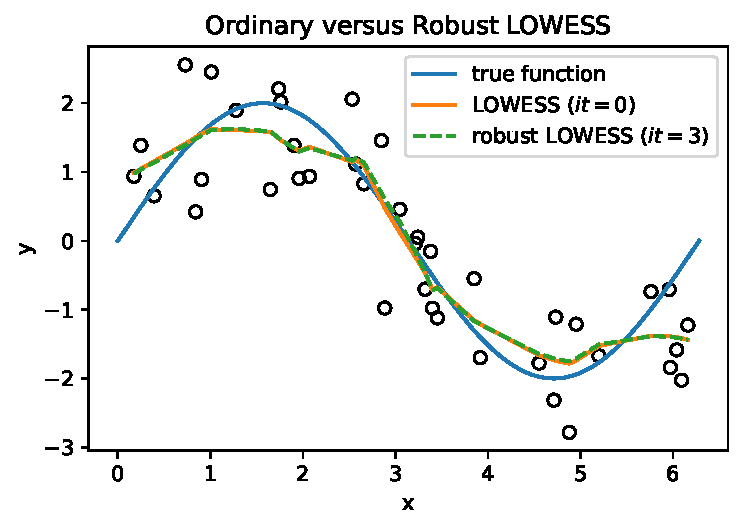
\includegraphics[keepaspectratio]{contents/2/kernel_files/figure-pdf/cell-23-output-1.pdf}}

The two fitted curves are quite similar because this dataset does not
contain any strong outliers. To make the effect of robustification
easier to see, we manually add a few outliers to a copy of the response
values.

\begin{Shaded}
\begin{Highlighting}[]
\NormalTok{y\_outlier }\OperatorTok{=}\NormalTok{ y.copy()}
\NormalTok{outlier\_indices }\OperatorTok{=}\NormalTok{ np.argsort(X)[[}\DecValTok{8}\NormalTok{, }\DecValTok{20}\NormalTok{, }\DecValTok{32}\NormalTok{]]}
\NormalTok{y\_outlier[outlier\_indices] }\OperatorTok{+=}\NormalTok{ [}\DecValTok{5}\NormalTok{, }\OperatorTok{{-}}\DecValTok{6}\NormalTok{, }\DecValTok{5}\NormalTok{]}

\NormalTok{lowess\_standard\_outlier }\OperatorTok{=}\NormalTok{ lowess(}
\NormalTok{    endog}\OperatorTok{=}\NormalTok{y\_outlier, exog}\OperatorTok{=}\NormalTok{X, frac}\OperatorTok{=}\FloatTok{0.25}\NormalTok{, it}\OperatorTok{=}\DecValTok{0}\NormalTok{, return\_sorted}\OperatorTok{=}\VariableTok{True}
\NormalTok{)}

\NormalTok{lowess\_robust\_outlier }\OperatorTok{=}\NormalTok{ lowess(}
\NormalTok{    endog}\OperatorTok{=}\NormalTok{y\_outlier, exog}\OperatorTok{=}\NormalTok{X, frac}\OperatorTok{=}\FloatTok{0.25}\NormalTok{, it}\OperatorTok{=}\DecValTok{3}\NormalTok{, return\_sorted}\OperatorTok{=}\VariableTok{True}
\NormalTok{)}
\end{Highlighting}
\end{Shaded}

We now compare ordinary and robust LOWESS on the data with outliers.

\begin{Shaded}
\begin{Highlighting}[]
\NormalTok{plt.scatter(X, y\_outlier, s}\OperatorTok{=}\DecValTok{35}\NormalTok{, facecolors}\OperatorTok{=}\StringTok{"none"}\NormalTok{, edgecolors}\OperatorTok{=}\StringTok{"black"}\NormalTok{)}
\NormalTok{plt.scatter(}
\NormalTok{    X[outlier\_indices],}
\NormalTok{    y\_outlier[outlier\_indices],}
\NormalTok{    s}\OperatorTok{=}\DecValTok{55}\NormalTok{,}
\NormalTok{    color}\OperatorTok{=}\StringTok{"C1"}\NormalTok{,}
\NormalTok{    label}\OperatorTok{=}\StringTok{"added outliers"}\NormalTok{,}
\NormalTok{    zorder}\OperatorTok{=}\DecValTok{3}\NormalTok{,}
\NormalTok{)}
\NormalTok{plt.plot(X\_grid, }\DecValTok{2} \OperatorTok{*}\NormalTok{ np.sin(X\_grid), label}\OperatorTok{=}\StringTok{"true function"}\NormalTok{)}
\NormalTok{plt.plot(}
\NormalTok{    lowess\_standard\_outlier[:, }\DecValTok{0}\NormalTok{],}
\NormalTok{    lowess\_standard\_outlier[:, }\DecValTok{1}\NormalTok{],}
\NormalTok{    label}\OperatorTok{=}\StringTok{"LOWESS ($it=0$)"}\NormalTok{,}
\NormalTok{)}
\NormalTok{plt.plot(}
\NormalTok{    lowess\_robust\_outlier[:, }\DecValTok{0}\NormalTok{],}
\NormalTok{    lowess\_robust\_outlier[:, }\DecValTok{1}\NormalTok{],}
\NormalTok{    linestyle}\OperatorTok{=}\StringTok{"{-}{-}"}\NormalTok{,}
\NormalTok{    label}\OperatorTok{=}\StringTok{"robust LOWESS ($it=3$)"}\NormalTok{,}
\NormalTok{)}
\NormalTok{plt.xlabel(}\StringTok{"x"}\NormalTok{)}
\NormalTok{plt.ylabel(}\StringTok{"y"}\NormalTok{)}
\NormalTok{plt.title(}\StringTok{"Ordinary versus Robust LOWESS with Outliers"}\NormalTok{)}
\NormalTok{plt.legend()}\OperatorTok{;}
\end{Highlighting}
\end{Shaded}

\pandocbounded{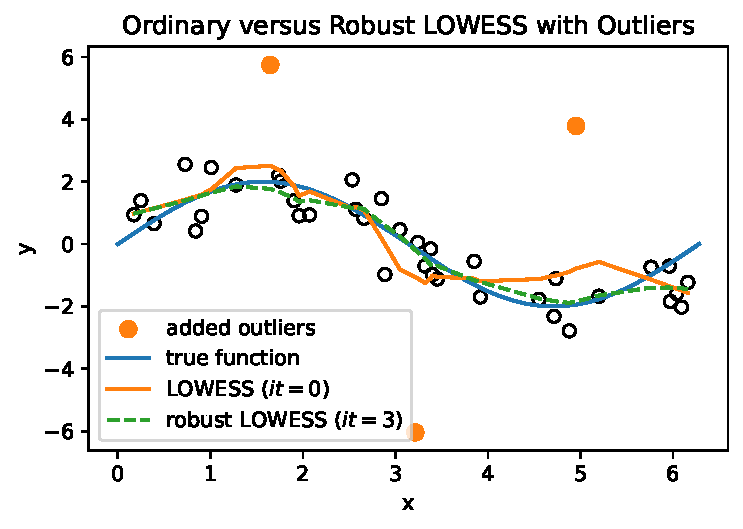
\includegraphics[keepaspectratio]{contents/2/kernel_files/figure-pdf/cell-25-output-1.pdf}}

\subsubsection{\texorpdfstring{Choosing
\texttt{frac}}{Choosing frac}}\label{choosing-frac}

The parameter \texttt{frac} controls the amount of smoothing.

\begin{itemize}
\tightlist
\item
  Smaller \texttt{frac} uses fewer nearby observations and produces a
  more flexible curve.
\item
  Larger \texttt{frac} uses more nearby observations and produces a
  smoother curve.
\end{itemize}

The span parameter \texttt{frac} can be selected by cross-validation
when prediction accuracy is the main goal. However, LOWESS is often used
as an exploratory visualization tool, so in practice \texttt{frac} is
frequently chosen by comparing several values visually.

\begin{Shaded}
\begin{Highlighting}[]
\ImportTok{from}\NormalTok{ statsmodels.nonparametric.smoothers\_lowess }\ImportTok{import}\NormalTok{ lowess}

\NormalTok{fracs }\OperatorTok{=}\NormalTok{ [}\FloatTok{0.1}\NormalTok{, }\FloatTok{0.25}\NormalTok{, }\FloatTok{0.5}\NormalTok{, }\FloatTok{0.75}\NormalTok{]}

\NormalTok{plt.scatter(X, y, s}\OperatorTok{=}\DecValTok{25}\NormalTok{, facecolors}\OperatorTok{=}\StringTok{"none"}\NormalTok{, edgecolors}\OperatorTok{=}\StringTok{"black"}\NormalTok{, alpha}\OperatorTok{=}\FloatTok{0.6}\NormalTok{)}

\ControlFlowTok{for}\NormalTok{ frac }\KeywordTok{in}\NormalTok{ fracs:}
\NormalTok{    result }\OperatorTok{=}\NormalTok{ lowess(endog}\OperatorTok{=}\NormalTok{y, exog}\OperatorTok{=}\NormalTok{X, frac}\OperatorTok{=}\NormalTok{frac, it}\OperatorTok{=}\DecValTok{0}\NormalTok{, return\_sorted}\OperatorTok{=}\VariableTok{True}\NormalTok{)}
\NormalTok{    plt.plot(result[:, }\DecValTok{0}\NormalTok{], result[:, }\DecValTok{1}\NormalTok{], linewidth}\OperatorTok{=}\DecValTok{2}\NormalTok{, label}\OperatorTok{=}\SpecialStringTok{f"frac=}\SpecialCharTok{\{}\NormalTok{frac}\SpecialCharTok{\}}\SpecialStringTok{"}\NormalTok{)}

\NormalTok{plt.xlabel(}\StringTok{"x"}\NormalTok{)}
\NormalTok{plt.ylabel(}\StringTok{"y"}\NormalTok{)}
\NormalTok{plt.title(}\StringTok{"Choosing frac by Visual Inspection"}\NormalTok{)}
\NormalTok{plt.legend()}
\end{Highlighting}
\end{Shaded}

\pandocbounded{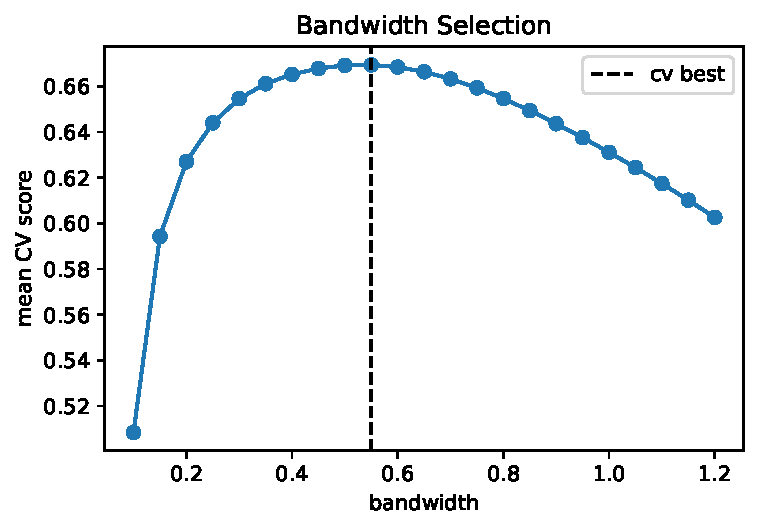
\includegraphics[keepaspectratio]{contents/2/kernel_files/figure-pdf/cell-26-output-1.pdf}}

Smaller values of \texttt{frac} produce more flexible curves that may
follow noise, while larger values produce smoother curves that may miss
local structure. The goal is to find a value that captures the overall
pattern without introducing excessive variability.

The curve with \texttt{frac=0.1} follows many small fluctuations and
appears to be fitting noise. The curve with \texttt{frac=0.75} is
heavily smoothed and begins to miss local features of the data. Values
between 0.25 and 0.5 provide a reasonable compromise, preserving the
overall trend while avoiding excessive variability.

\begin{tcolorbox}[enhanced jigsaw, arc=.35mm, bottomrule=.15mm, bottomtitle=1mm, breakable, colback=white, colbacktitle=quarto-callout-note-color!10!white, colframe=quarto-callout-note-color-frame, coltitle=black, left=2mm, leftrule=.75mm, opacityback=0, opacitybacktitle=0.6, rightrule=.15mm, title=\textcolor{quarto-callout-note-color}{\faInfo}\hspace{0.5em}{Visual bandwidth selection}, titlerule=0mm, toprule=.15mm, toptitle=1mm]

Kernel smoothing methods involve a smoothing parameter:

\begin{itemize}
\tightlist
\item
  bandwidth \(h\) in kernel density estimation and kernel regression;
\item
  span \texttt{frac} in LOWESS.
\end{itemize}

Smaller values produce more flexible estimates with lower bias but
higher variance. Larger values produce smoother estimates with higher
bias but lower variance.

When visualization is the primary goal, a common strategy is to compare
several values and choose the smallest amount of smoothing that removes
obvious noise while preserving the main structure of the data.

\end{tcolorbox}

\subsection{Multiple Dimensions}\label{multiple-dimensions}

For \(x_i\in\mathbb R^p\), a common Gaussian kernel is

\[
K_h(x,x_i)
\propto
\exp\left(
-\frac{\|x-x_i\|^2}{2h^2}
\right).
\]

This is similar to KNN in that it relies on distances in feature space.
Therefore, scaling matters.

In multiple dimensions, kernel smoothing faces the curse of
dimensionality. As \(p\) increases, local neighborhoods become sparse.
To get enough nearby points, the bandwidth must grow, which increases
bias.

For \(p\) dimensions, bandwidth rates are often of order

\[
n^{-1/(p+4)}.
\]

This gets slower as \(p\) increases, which is another way to see the
curse of dimensionality.

\begin{tcolorbox}[enhanced jigsaw, arc=.35mm, bottomrule=.15mm, bottomtitle=1mm, breakable, colback=white, colbacktitle=quarto-callout-caution-color!10!white, colframe=quarto-callout-caution-color-frame, coltitle=black, left=2mm, leftrule=.75mm, opacityback=0, opacitybacktitle=0.6, rightrule=.15mm, title=\textcolor{quarto-callout-caution-color}{\faFire}\hspace{0.5em}{Bandwidth conventions}, titlerule=0mm, toprule=.15mm, toptitle=1mm]

Different software packages may define bandwidth differently. Some use a
raw scale \(h\) inside the kernel. Others use a span, a nearest-neighbor
fraction, or an internally rescaled bandwidth. Always check the
documentation before comparing bandwidth values across implementations.

\end{tcolorbox}

\section{\texorpdfstring{Optional: Building a Custom \texttt{sklearn}
Regressor}{Optional: Building a Custom sklearn Regressor}}\label{optional-building-a-custom-sklearn-regressor}

Click to expand.

\subsection{Nadaraya-Watson
estimator}\label{nadaraya-watson-estimator-1}

Recall the formula for the Nadaraya--Watson estimator: \[
\hat f(x)
=
\frac{
\sum_{i=1}^n K_h(x,x_i)y_i
}{
\sum_{i=1}^n K_h(x,x_i)
}.
\] We can translate this formula directly into a Python function.

\begin{Shaded}
\begin{Highlighting}[]
\KeywordTok{def}\NormalTok{ kernel\_regression\_predict(X, y, X\_new, bandwidth):}
\NormalTok{    diff }\OperatorTok{=}\NormalTok{ X\_new[:, }\VariableTok{None}\NormalTok{] }\OperatorTok{{-}}\NormalTok{ X[}\VariableTok{None}\NormalTok{, :]}
\NormalTok{    weights }\OperatorTok{=}\NormalTok{ np.exp(}\OperatorTok{{-}}\FloatTok{0.5} \OperatorTok{*}\NormalTok{ (diff }\OperatorTok{/}\NormalTok{ bandwidth) }\OperatorTok{**} \DecValTok{2}\NormalTok{)}
\NormalTok{    weights }\OperatorTok{=}\NormalTok{ weights }\OperatorTok{/}\NormalTok{ weights.}\BuiltInTok{sum}\NormalTok{(axis}\OperatorTok{=}\DecValTok{1}\NormalTok{, keepdims}\OperatorTok{=}\VariableTok{True}\NormalTok{)}
    \ControlFlowTok{return}\NormalTok{ weights }\OperatorTok{@}\NormalTok{ y}

\NormalTok{h }\OperatorTok{=} \FloatTok{0.25}
\NormalTok{y\_kernel }\OperatorTok{=}\NormalTok{ kernel\_regression\_predict(X, y, X\_grid, bandwidth}\OperatorTok{=}\NormalTok{h)}
\end{Highlighting}
\end{Shaded}

Here \texttt{diff\ =\ X\_new{[}:,\ None{]}\ -\ X{[}None,\ :{]}} uses
\texttt{numpy} broadcasting to create a matrix of pairwise differences.
It was briefly discussed in Section~\ref{sec-common_operations}. If
\texttt{X\_new} contains \(m\) points and \texttt{X} contains \(n\)
points, then \texttt{diff} has shape \((m,n)\), where the \((i,j)\)
entry is the difference between the \(i\)th prediction point and the
\(j\)th training point.

This simple function is useful for understanding the algorithm. We now
turn it into a custom \texttt{sklearn} regressor so that it can be used
with tools such as \texttt{GridSearchCV}.

\subsection{Guidelines for Developing a Custom Scikit-learn
Regressor}\label{guidelines-for-developing-a-custom-scikit-learn-regressor}

According to the
\href{https://scikit-learn.org/stable/developers/develop.html}{official
\texttt{sklearn} developer guide}, a custom regression estimator should
inherit from both \texttt{RegressorMixin} and \texttt{BaseEstimator} to
integrate smoothly with the \texttt{sklearn} ecosystem. A minimal
regressor typically implements three methods: \texttt{\_\_init\_\_},
\texttt{fit}, and \texttt{predict}.

\begin{enumerate}
\def\labelenumi{\arabic{enumi}.}
\tightlist
\item
  The Role of \texttt{BaseEstimator}
\end{enumerate}

\texttt{BaseEstimator} provides the infrastructure that allows an
estimator to work with \texttt{sklearn} utilities such as pipelines,
model selection tools, and cloning.

\begin{itemize}
\tightlist
\item
  It automatically implements \texttt{.get\_params()} and
  \texttt{.set\_params()}. These methods are required by tools such as
  \texttt{GridSearchCV}, \texttt{RandomizedSearchCV}, and
  \texttt{Pipeline}.
\item
  The \texttt{\_\_init\_\_} method should only store the supplied
  parameters. Every constructor argument should be assigned directly to
  an attribute with the same name, such as
  \texttt{self.bandwidth\ =\ bandwidth}.
\item
  The constructor should not

  \begin{itemize}
  \tightlist
  \item
    modify parameter values,
  \item
    perform input validation,
  \item
    perform data-dependent computations,
  \item
    store training data.
  \end{itemize}
\item
  Data validation and data-dependent computations should be performed
  inside \texttt{fit()} or \texttt{predict()}.
\end{itemize}

By following these rules, the estimator automatically supports:

\begin{itemize}
\tightlist
\item
  cloning via \texttt{sklearn.base.clone},
\item
  parameter inspection,
\item
  compatibility with pipelines and model-selection tools.
\end{itemize}

\begin{enumerate}
\def\labelenumi{\arabic{enumi}.}
\setcounter{enumi}{1}
\tightlist
\item
  The Role of \texttt{RegressorMixin}
\end{enumerate}

\begin{itemize}
\tightlist
\item
  \texttt{RegressorMixin} identifies the estimator as a regression model
  and provides a default scoring method.
\item
  The mixin automatically implements the \texttt{.score()} method, which
  returns the coefficient of determination, or \(R^2\), by default.
\item
  A regressor should implement \texttt{.fit(X,\ y)} and
  \texttt{.predict(X)}, where \texttt{y} is usually a numerical target
  variable.
\item
  Attributes estimated from the training data should end with a trailing
  underscore, such as \texttt{self.coef\_}, \texttt{self.intercept\_},
  or \texttt{self.X\_train\_}. This convention distinguishes learned
  quantities from hyperparameters.
\item
  The \texttt{fit()} method should always return the estimator itself.
  This allows method chaining such as
  \texttt{model.fit(X,\ y).predict(X\_new)}.
\end{itemize}

\begin{enumerate}
\def\labelenumi{\arabic{enumi}.}
\setcounter{enumi}{2}
\tightlist
\item
  Recommended Practices
\end{enumerate}

\texttt{sklearn} provides \texttt{validate\_data} and
\texttt{check\_is\_fitted} from \texttt{sklearn.utils.validation} to
perform input validation and fitted-state checks consistently with
built-in estimators.

Although these utilities are not required for simple educational
examples, they are recommended for production-quality estimators.

In addition, it is recommended to validate all arguments besides the
input dataset. For example, the bandwidth in our case should be
positive.

\subsection{\texorpdfstring{\texttt{sklearn}
regressor}{sklearn regressor}}\label{sklearn-regressor}

\begin{Shaded}
\begin{Highlighting}[]
\ImportTok{from}\NormalTok{ sklearn.base }\ImportTok{import}\NormalTok{ BaseEstimator, RegressorMixin}
\ImportTok{from}\NormalTok{ sklearn.utils.validation }\ImportTok{import}\NormalTok{ validate\_data, check\_is\_fitted}

\KeywordTok{class}\NormalTok{ NadarayaWatsonRegressor(RegressorMixin, BaseEstimator):}
    \KeywordTok{def} \FunctionTok{\_\_init\_\_}\NormalTok{(}\VariableTok{self}\NormalTok{, bandwidth}\OperatorTok{=}\FloatTok{1.0}\NormalTok{):}
        \VariableTok{self}\NormalTok{.bandwidth }\OperatorTok{=}\NormalTok{ bandwidth}

    \KeywordTok{def}\NormalTok{ fit(}\VariableTok{self}\NormalTok{, X, y):}
        \ControlFlowTok{if} \VariableTok{self}\NormalTok{.bandwidth }\OperatorTok{\textless{}=} \DecValTok{0}\NormalTok{:}
            \ControlFlowTok{raise} \PreprocessorTok{ValueError}\NormalTok{(}\StringTok{"bandwidth must be positive."}\NormalTok{)}
\NormalTok{        X, y }\OperatorTok{=}\NormalTok{ validate\_data(}\VariableTok{self}\NormalTok{, X, y, y\_numeric}\OperatorTok{=}\VariableTok{True}\NormalTok{)}
        \VariableTok{self}\NormalTok{.X\_train\_ }\OperatorTok{=}\NormalTok{ X}
        \VariableTok{self}\NormalTok{.y\_train\_ }\OperatorTok{=}\NormalTok{ y}
        \ControlFlowTok{return} \VariableTok{self}

    \KeywordTok{def}\NormalTok{ predict(}\VariableTok{self}\NormalTok{, X\_new):}
\NormalTok{        check\_is\_fitted(}\VariableTok{self}\NormalTok{, [}\StringTok{"X\_train\_"}\NormalTok{, }\StringTok{"y\_train\_"}\NormalTok{])}
\NormalTok{        X\_new }\OperatorTok{=}\NormalTok{ validate\_data(}\VariableTok{self}\NormalTok{, X\_new, reset}\OperatorTok{=}\VariableTok{False}\NormalTok{)}

\NormalTok{        diff }\OperatorTok{=}\NormalTok{ X\_new[:, }\VariableTok{None}\NormalTok{, :] }\OperatorTok{{-}} \VariableTok{self}\NormalTok{.X\_train\_[}\VariableTok{None}\NormalTok{, :, :]}
\NormalTok{        squared\_distances }\OperatorTok{=}\NormalTok{ np.}\BuiltInTok{sum}\NormalTok{(diff}\OperatorTok{**}\DecValTok{2}\NormalTok{, axis}\OperatorTok{=}\DecValTok{2}\NormalTok{)}

\NormalTok{        weights }\OperatorTok{=}\NormalTok{ np.exp(}\OperatorTok{{-}}\FloatTok{0.5} \OperatorTok{*}\NormalTok{ squared\_distances }\OperatorTok{/} \VariableTok{self}\NormalTok{.bandwidth}\OperatorTok{**}\DecValTok{2}\NormalTok{)}
\NormalTok{        weights }\OperatorTok{=}\NormalTok{ weights }\OperatorTok{/}\NormalTok{ weights.}\BuiltInTok{sum}\NormalTok{(axis}\OperatorTok{=}\DecValTok{1}\NormalTok{, keepdims}\OperatorTok{=}\VariableTok{True}\NormalTok{)}

        \ControlFlowTok{return}\NormalTok{ weights }\OperatorTok{@} \VariableTok{self}\NormalTok{.y\_train\_}
\end{Highlighting}
\end{Shaded}

This \texttt{predict} method is closely related to the
\texttt{kernel\_regression\_predict} function defined earlier. The main
difference, apart from the validation checks, is that this version
supports multidimensional input. That is, \texttt{X} may contain more
than one feature column.

\subsection{Grid search}\label{grid-search}

With the custom regressor, we can seamlessly connect it to the
\texttt{sklearn} ecosystem. For example, we can start to perform grid
search.

\begin{Shaded}
\begin{Highlighting}[]
\ImportTok{from}\NormalTok{ sklearn.model\_selection }\ImportTok{import}\NormalTok{ GridSearchCV}

\NormalTok{bandwidth\_grid }\OperatorTok{=}\NormalTok{ \{}\StringTok{"bandwidth"}\NormalTok{: np.linspace(}\FloatTok{0.1}\NormalTok{, }\FloatTok{1.2}\NormalTok{, }\DecValTok{23}\NormalTok{)\}}

\NormalTok{grid }\OperatorTok{=}\NormalTok{ GridSearchCV(NadarayaWatsonRegressor(), param\_grid}\OperatorTok{=}\NormalTok{bandwidth\_grid, cv}\OperatorTok{=}\DecValTok{5}\NormalTok{)}

\NormalTok{grid.fit(X.reshape(}\OperatorTok{{-}}\DecValTok{1}\NormalTok{, }\DecValTok{1}\NormalTok{), y)}
\NormalTok{grid.best\_params\_}
\end{Highlighting}
\end{Shaded}

\begin{verbatim}
{'bandwidth': np.float64(0.5499999999999999)}
\end{verbatim}

Plot the cross-validation curve.

\begin{Shaded}
\begin{Highlighting}[]
\NormalTok{cv\_score }\OperatorTok{=}\NormalTok{ grid.cv\_results\_[}\StringTok{"mean\_test\_score"}\NormalTok{]}
\NormalTok{bandwidth\_values }\OperatorTok{=}\NormalTok{ bandwidth\_grid[}\StringTok{"bandwidth"}\NormalTok{]}

\NormalTok{plt.plot(bandwidth\_values, cv\_score, marker}\OperatorTok{=}\StringTok{"o"}\NormalTok{)}
\NormalTok{plt.axvline(grid.best\_params\_[}\StringTok{"bandwidth"}\NormalTok{], color}\OperatorTok{=}\StringTok{"black"}\NormalTok{, linestyle}\OperatorTok{=}\StringTok{"{-}{-}"}\NormalTok{, label}\OperatorTok{=}\StringTok{\textquotesingle{}cv best\textquotesingle{}}\NormalTok{)}
\NormalTok{plt.xlabel(}\StringTok{"bandwidth"}\NormalTok{)}
\NormalTok{plt.ylabel(}\StringTok{"mean CV score"}\NormalTok{)}
\NormalTok{plt.title(}\StringTok{"Bandwidth Selection"}\NormalTok{)}
\NormalTok{plt.legend()}\OperatorTok{;}
\end{Highlighting}
\end{Shaded}

\pandocbounded{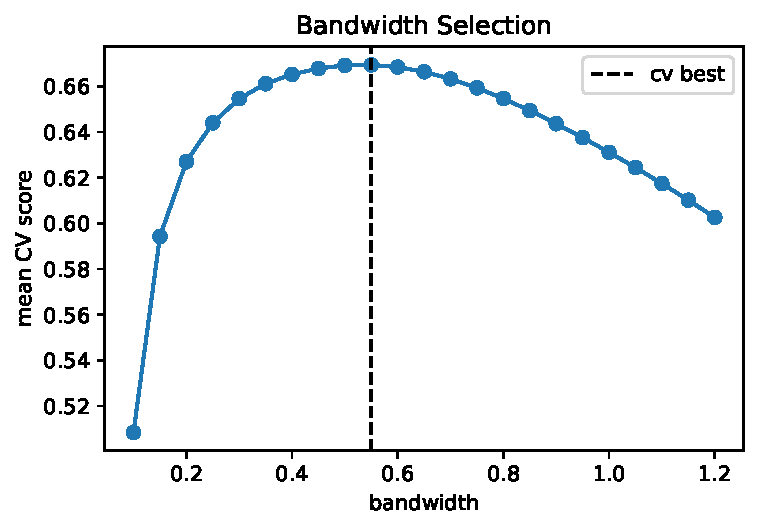
\includegraphics[keepaspectratio]{contents/2/kernel_files/figure-pdf/cell-30-output-1.pdf}}

Fit the selected model.

\begin{Shaded}
\begin{Highlighting}[]
\NormalTok{best\_kernel }\OperatorTok{=}\NormalTok{ grid.best\_estimator\_}
\NormalTok{y\_best }\OperatorTok{=}\NormalTok{ best\_kernel.predict(X\_grid.reshape(}\OperatorTok{{-}}\DecValTok{1}\NormalTok{, }\DecValTok{1}\NormalTok{))}

\NormalTok{plt.scatter(X, y, s}\OperatorTok{=}\DecValTok{35}\NormalTok{, facecolors}\OperatorTok{=}\StringTok{"none"}\NormalTok{, edgecolors}\OperatorTok{=}\StringTok{"black"}\NormalTok{)}
\NormalTok{plt.plot(X\_grid, }\DecValTok{2} \OperatorTok{*}\NormalTok{ np.sin(X\_grid), color}\OperatorTok{=}\StringTok{"C0"}\NormalTok{, label}\OperatorTok{=}\StringTok{"true function"}\NormalTok{)}
\NormalTok{plt.plot(X\_grid, y\_best, color}\OperatorTok{=}\StringTok{"C1"}\NormalTok{, linewidth}\OperatorTok{=}\DecValTok{2}\NormalTok{, label}\OperatorTok{=}\StringTok{"CV{-}selected fit"}\NormalTok{)}
\NormalTok{plt.xlabel(}\StringTok{"x"}\NormalTok{)}
\NormalTok{plt.ylabel(}\StringTok{"y"}\NormalTok{)}
\NormalTok{plt.title(}\SpecialStringTok{f"Selected Bandwidth = }\SpecialCharTok{\{}\NormalTok{grid}\SpecialCharTok{.}\NormalTok{best\_params\_[}\StringTok{\textquotesingle{}bandwidth\textquotesingle{}}\NormalTok{]}\SpecialCharTok{:.2f\}}\SpecialStringTok{"}\NormalTok{)}
\NormalTok{plt.legend()}\OperatorTok{;}
\end{Highlighting}
\end{Shaded}

\pandocbounded{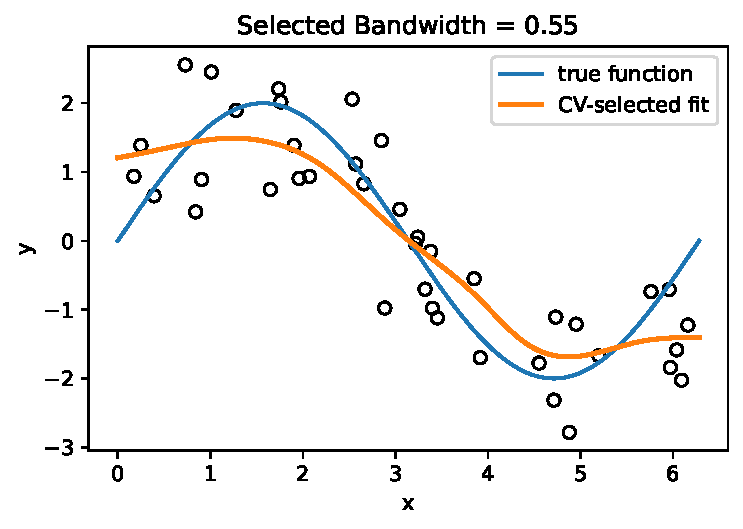
\includegraphics[keepaspectratio]{contents/2/kernel_files/figure-pdf/cell-31-output-1.pdf}}

\chapter{Tree-Based Methods}\label{tree-based-methods}

A decision tree is another nonparametric method, which learns a
collection of simple if-then rules directly from the data.

The basic idea is:

\begin{enumerate}
\def\labelenumi{\arabic{enumi}.}
\tightlist
\item
  Split the feature space into regions.
\item
  Continue splitting each region into smaller regions.
\item
  Use the observations inside each final region to make predictions.
\end{enumerate}

\section{Basic Tree Terminology}\label{basic-tree-terminology}

A decision tree recursively divides the training observations into
smaller groups. Each node is a position in the tree together with the
observations assigned to it.

\begin{itemize}
\tightlist
\item
  A node is a position in the tree. We use \(G\) to denote the set of
  training observations in a node, and \(|G|\) denotes the number of
  observations in that set. Equivalently, \(G\) identifies a subset of
  the rows of \(X\).
\item
  The root node is the node at the top of the tree. It contains all
  training observations.
\item
  A split applies a rule such as \(x_j\leq c\) to a node and divides it
  into two child nodes. The original node is their parent node.
\item
  An internal node, also called a decision node, is a node that has been
  split.
\item
  A leaf node, also called a terminal node, is a node that is not split
  further. Each leaf contains a final group of observations used to make
  a prediction.
\item
  The depth of a node is the number of parent-child connections
  traversed when moving from the root to that node. The root has depth
  0.
\item
  The depth of a tree is the largest depth among all nodes in the tree.
  Equivalently, it is the largest number of edges on any path from the
  root to a leaf.
\item
  A subtree consists of a node and all of its descendants. Pruning
  replaces a larger subtree with a leaf.
\item
  A binary tree is a tree in which each internal node has two children.
  CART constructs binary trees. Note that there are other algorithms
  that can build trees, and they may not create binary trees.
\end{itemize}

For classification, a leaf usually predicts the most common class or the
class proportions among its observations. For regression, a leaf usually
predicts the mean response among its observations. A classification node
is pure when all its observations belong to the same class.

\begin{example}[Example: A Classification
Tree]\protect\hypertarget{exm-}{}\label{exm-}

~

\pandocbounded{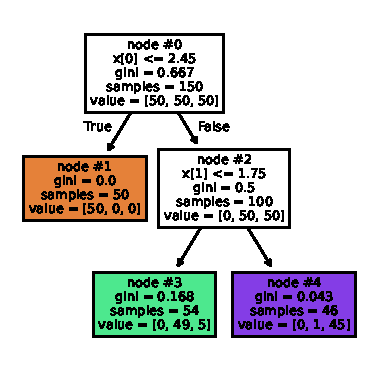
\includegraphics[keepaspectratio]{contents/2/tree_files/figure-pdf/cell-2-output-1.pdf}}

This is a classification tree. The tree repeatedly asks simple questions
such as

\begin{itemize}
\tightlist
\item
  Is \texttt{x{[}0{]}\ \textless{}=\ 2.45}?
\item
  Is \texttt{x{[}1{]}\ \textless{}=\ 1.75}?
\end{itemize}

Each split divides the feature space into smaller regions.

This tree actually create the following splits in the feature space.

\pandocbounded{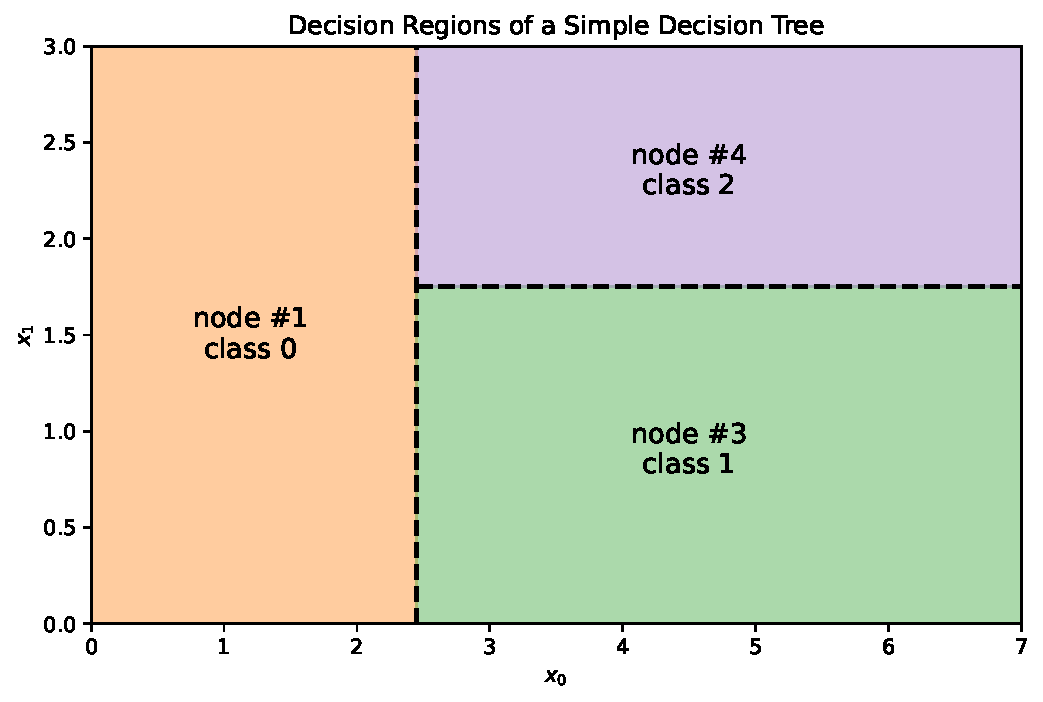
\includegraphics[keepaspectratio]{contents/2/tree_files/figure-pdf/cell-3-output-1.pdf}}

We could also go over all basic terminologies in this example.

\begin{itemize}
\tightlist
\item
  Node \#0 is the root node. It contains all 150 observations in the
  dataset and has depth 0.
\item
  Node \#0 is an internal node. Its split sends observations to node \#1
  or node \#2, which are its child nodes.
\item
  Node \#2 is also an internal node. It is a child of node \#0 and the
  parent of nodes \#3 and \#4.
\item
  Nodes \#1, \#3, and \#4 are leaf nodes because they are not split
  further. Their depths are 1, 2, and 2, respectively.
\item
  The depth of this tree is 2, which is the largest depth among its
  nodes.
\item
  This is a binary tree because every internal node has exactly two
  children.
\item
  One example of splits: node \#0 uses the split \(x_0\leq 2.45\) to
  send observations to node \#1 or node \#2.
\item
  One example of subtree: the subtree rooted at node \#2 consists of
  nodes \#2, \#3, and \#4.
\item
  Each leaf makes a prediction using the observations it contains. For
  example, node \#1 predicts class 0, the most common class among its
  observations.
\item
  Node \#1 is pure because all observations in it belong to class 0. Its
  Gini impurity is therefore 0.
\end{itemize}

\end{example}

Based on the idea of a decision tree, a tree makes decisions by
repeatedly asking questions of the form \(x_j \leq c\). Therefore, a
tree has two important properties:

\begin{itemize}
\tightlist
\item
  It depends directly on the original features.
\item
  The scale of a feature is usually not important.
\end{itemize}

As a result, we should expect that a tree is:

\begin{itemize}
\tightlist
\item
  sensitive to feature construction or feature combinations: A tree can
  only split on the features that are provided. If the useful signal is
  hidden in a combination such as \(x_1+x_2\) or \(x_1x_2\), a tree may
  need many splits to approximate that relationship.
\item
  not sensitive to monotone transformations of a feature: For example,
  replacing \(x\) by \(\log(x)\) or \(2x+5\) does not change the
  ordering of the observations. Since tree splits mainly depend on
  ordering, the tree can usually produce an equivalent split after the
  transformation.
\end{itemize}

\section{CART: Classification and Regression
Trees}\label{cart-classification-and-regression-trees}

There are many algorithms for constructing decision trees. The most
common one is called CART (Classification and Regression Trees) {[}7{]}.

CART has the following properties:

\begin{itemize}
\tightlist
\item
  It creates only binary splits;
\item
  It can perform both classification and regression tasks:

  \begin{itemize}
  \tightlist
  \item
    For classification, common splitting criteria include Gini impurity
    and entropy;
  \item
    For regression, common splitting criteria include residual sum of
    squares (RSS) and mean squared error (MSE).
  \end{itemize}
\end{itemize}

\subsection{Splitting a Dataset}\label{splitting-a-dataset}

At each step, CART searches over possible splits and chooses the split
that produces the largest reduction in impurity (or prediction error).

\begin{tcolorbox}[enhanced jigsaw, arc=.35mm, bottomrule=.15mm, bottomtitle=1mm, breakable, colback=white, colbacktitle=quarto-callout-note-color!10!white, colframe=quarto-callout-note-color-frame, coltitle=black, left=2mm, leftrule=.75mm, opacityback=0, opacitybacktitle=0.6, rightrule=.15mm, title=\textcolor{quarto-callout-note-color}{\faInfo}\hspace{0.5em}{Algorithm: Split the Dataset}, titlerule=0mm, toprule=.15mm, toptitle=1mm]

\textbf{Inputs:} A dataset \(S={[\text{features},\text{target}]}\)

\textbf{Outputs:} The best split \((k,t)\)

\begin{enumerate}
\def\labelenumi{\arabic{enumi}.}
\tightlist
\item
  For each feature \(x_k\):

  \begin{enumerate}
  \def\labelenumii{\arabic{enumii}.}
  \tightlist
  \item
    For each candidate split value \(t\):

    \begin{enumerate}
    \def\labelenumiii{\arabic{enumiii}.}
    \tightlist
    \item
      Split the dataset into two subsets:
      \(G_l=\qty{\text{data with }x_k\le t}\),
      \(G_r=\qty{\text{data with }x_k>t}\).
    \item
      Compute the split cost function \(J(k,t)\)
    \item
      Keep the best split found so far
    \end{enumerate}
  \end{enumerate}
\item
  Return the split \((k,t)\) with the smallest cost
\end{enumerate}

\end{tcolorbox}

The splitting algorithm is applied recursively.

\begin{tcolorbox}[enhanced jigsaw, arc=.35mm, bottomrule=.15mm, bottomtitle=1mm, breakable, colback=white, colbacktitle=quarto-callout-note-color!10!white, colframe=quarto-callout-note-color-frame, coltitle=black, left=2mm, leftrule=.75mm, opacityback=0, opacitybacktitle=0.6, rightrule=.15mm, title=\textcolor{quarto-callout-note-color}{\faInfo}\hspace{0.5em}{Algorithm: CART}, titlerule=0mm, toprule=.15mm, toptitle=1mm]

\textbf{Inputs:} A labeled dataset \(S\) and a maximal tree depth
\texttt{max\_depth}

\textbf{Outputs:} A decision tree

\begin{enumerate}
\def\labelenumi{\arabic{enumi}.}
\tightlist
\item
  Start with the original dataset \(S\)
\item
  If the node is not pure and stopping conditions are not met:

  \begin{enumerate}
  \def\labelenumii{\arabic{enumii}.}
  \tightlist
  \item
    Find the best split
  \item
    Split the node into: \(G_l\) and \(G_r\)
  \item
    Apply the same procedure recursively to both child nodes
  \end{enumerate}
\item
  Stop when:

  \begin{itemize}
  \tightlist
  \item
    the maximal tree depth is reached, or
  \item
    the node becomes pure, or
  \item
    further splitting is impossible
  \end{itemize}
\end{enumerate}

\end{tcolorbox}

When making predictions, a classification tree uses the most common
class label in a region as the predicted value, while a regression tree
uses the mean of the response values in the region as the predicted
value.

\subsection{Classification Trees: Gini
Impurity}\label{classification-trees-gini-impurity}

Classification trees are used when the response variable is categorical.
A classification tree partitions the feature space into piecewise
constant regions, where each region predicts either a class label or
class probabilities.

In these notes, we use Gini impurity to measure the quality of a split.

Assume that a node contains \(n\) observations divided into \(K\)
classes. Let \(p_i=\frac{n_i}{n}\) be the proportion of class \(i\). If
we classify observations according to the class proportions:

\begin{itemize}
\tightlist
\item
  the probability an observation belongs to class \(i\) is \(p_i\)
\item
  the probability we incorrectly classify it is \(1-p_i\)
\end{itemize}

Therefore the probability of misclassifying an observation from class
\(i\) is

\[
p_i(1-p_i).
\]

Summing over all classes gives

\[
\sum_{i=1}^K p_i(1-p_i).
\]

Since

\[
\sum_{i=1}^K p_i=1,
\]

we obtain

\[
\gini
=\sum_{i=1}^K p_i(1-p_i)
=1-\sum_{i=1}^K p_i^2.
\]

\begin{definition}[Gini
Impurity]\protect\hypertarget{def-gini}{}\label{def-gini}

The \textbf{Gini impurity} of a node is

\[
\gini
=1-\sum_{i=1}^K p_i^2,
\]

where \(p_i\) is the proportion of class \(i\) inside the node.

\end{definition}

\begin{example}[Pure node]\protect\hypertarget{exm-}{}\label{exm-}

Suppose a node contains observations from only one class.

Then one of the probabilities equals 1 and all others equal 0.

Therefore

\[
\gini=1-1^2=0.
\]

This is the minimum possible impurity.

A node with Gini impurity 0 is called a pure node.

\end{example}

\begin{example}[Two-Class
Example]\protect\hypertarget{exm-}{}\label{exm-}

Suppose we have two classes.

Let

\[
p_2=1-p_1.
\]

Then

\[
\gini
=1-p_1^2-(1-p_1)^2
=2p_1-2p_1^2.
\]

When:

\begin{itemize}
\tightlist
\item
  \(p_1=0\) or \(1\), the impurity is 0;
\item
  \(p_1=0.5\), the impurity is maximized.
\end{itemize}

Therefore, impurity is largest when the classes are perfectly balanced.

\end{example}

The impurity of a node alone is not enough. CART evaluates a split by
examining the impurity of the child nodes after splitting.

Suppose a node \(G\) is split into \(G_l\) and \(G_r\). The split cost
is

\[
J
=\frac{|G_l|}{|G|}\gini(G_l)
+\frac{|G_r|}{|G|}\gini(G_r).
\]

A good split produces child nodes with low impurity, ideally creating
nodes that are close to pure.

The cost of a tree is obtained by applying this weighting recursively
down to the leaves. It is therefore a weighted sum of the Gini impurity
of each leaf, with weights given by the proportion of samples falling
into that leaf.

\begin{tcolorbox}[enhanced jigsaw, arc=.35mm, bottomrule=.15mm, bottomtitle=1mm, breakable, colback=white, colbacktitle=quarto-callout-note-color!10!white, colframe=quarto-callout-note-color-frame, coltitle=black, left=2mm, leftrule=.75mm, opacityback=0, opacitybacktitle=0.6, rightrule=.15mm, title=\textcolor{quarto-callout-note-color}{\faInfo}\hspace{0.5em}{Entropy}, titlerule=0mm, toprule=.15mm, toptitle=1mm]

Entropy is another popular impurity measure. Its formula is

\[
\mathrm{Entropy}
=-\sum_{i=1}^K p_i\log(p_i).
\]

Entropy and Gini impurity usually produce very similar trees.

Because Gini impurity is slightly simpler computationally and
conceptually, we mainly focus on it.

\end{tcolorbox}

\subsection{Regression Trees: RSS}\label{regression-trees-rss}

Regression trees are used when the response variable is quantitative.
Instead of predicting a class label, they predict numerical values.

Suppose a leaf node contains responses \(y_1\), \(y_2\), \(\ldots\),
\(y_n\). The prediction for that region is usually the sample mean: \[
\hat y
=\frac{1}{n}\sum_{i=1}^n y_i.
\]

Therefore, regression trees approximate the regression function using
piecewise constant regions.

For regression trees, CART typically minimizes the residual sum of
squares (RSS). Sometimes the mean squared error (MSE) is used instead.
Since MSE differs from RSS only by a constant scaling factor, minimizing
one is equivalent to minimizing the other.

Suppose a split divides the data into two regions \(G_l\) and \(G_r\).
The split cost is

\[
\rss
=
\sum_{i\in G_l}(y_i-\bar y_l)^2
+
\sum_{i\in G_r}(y_i-\bar y_r)^2,
\]

where \(\bar y_l\) and \(\bar y_r\) are the mean responses within the
two regions. The best split is the one that minimizes this quantity.

\subsection{Trees are local}\label{trees-are-local}

A tree makes predictions using only observations inside a small region
of the feature space. Suppose a tree partitions the feature space into
regions. The prediction at a point \(x\) depends only on the region
containing \(x\). As a result, tree predictions are local:

\begin{itemize}
\tightlist
\item
  nearby regions may have very different predictions
\item
  only observations in the same local region affect the prediction
\item
  changing distant observations usually does not affect the prediction
\end{itemize}

This is similar in spirit to KNN, where prediction also depends
primarily on nearby observations.

\subsection{Trees are nonlinear}\label{trees-are-nonlinear}

A tree creates many if-then rules. Because of these recursive splits:

\begin{itemize}
\tightlist
\item
  the prediction function can change abruptly
\item
  variable effects depend on the region
\item
  interactions are created automatically
\end{itemize}

The prediction surface is therefore discontinuous and piecewise
constant. Therefore, trees are nonlinear models.

\subsection{Automatic interaction
effects}\label{automatic-interaction-effects}

One important property of trees is that they automatically create
interaction effects.

For example, consider a tree with depth 3. One path through the tree may
look like:

\begin{itemize}
\tightlist
\item
  if \(x_1 \le 1\)
\item
  and \(x_2 \le 2\)
\item
  and \(x_3 \le 3\)
\item
  then predict \(y=1.1\)
\end{itemize}

Notice that the prediction depends on the combination of all three
conditions simultaneously. Therefore, the effect of one variable may
depend on the values of earlier splitting variables. In other words, the
effect of \(x_3\) is not independent of \(x_1\) and \(x_2\). The split
on \(x_3\) is only relevant inside the region defined by the earlier
splits.

Therefore, trees naturally model interactions between variables.

This is very different from a standard additive linear model such as

\[
f(x)=\beta_0+\beta_1x_1+\beta_2x_2+\beta_3x_3,
\]

where each variable contributes independently unless explicit
interaction terms like \(x_1x_2\) are manually added.

\section{Tuning hyperparameters}\label{tuning-hyperparameters}

Building a decision tree is the same as recursively splitting the
training dataset. If we are allowed to keep splitting it, almost every
leaf may become pure: its Gini impurity is 0 for classification, or all
observations in the leaf have the same response value for regression.

\begin{example}[ALMOST all leaves are
pure]\protect\hypertarget{exm-}{}\label{exm-}

~

Click to expand.

In this example, we let the tree grow as far as possible. It only stops
when (almost) all leaves are pure, even if a leaf contains only ONE
observation (like \#6 and \#11).

\pandocbounded{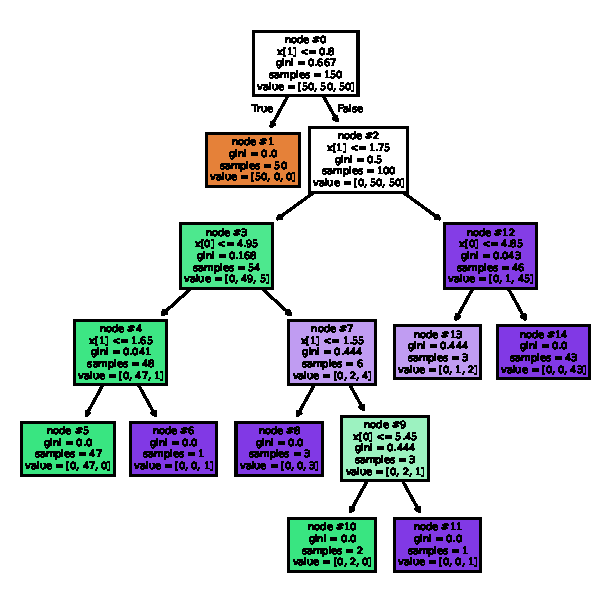
\includegraphics[keepaspectratio]{contents/2/tree_files/figure-pdf/cell-4-output-1.pdf}}

In this example there is one exception. \#13 node is not pure. We could
list all data in node \#13.

{\def\LTcaptype{none} % do not increment counter
\begin{longtable}[]{@{}llll@{}}
\toprule\noalign{}
& x{[}0{]} & x{[}1{]} & y \\
\midrule\noalign{}
\endhead
\bottomrule\noalign{}
\endlastfoot
0 & 4.8 & 1.8 & 1 \\
1 & 4.8 & 1.8 & 2 \\
2 & 4.8 & 1.8 & 2 \\
\end{longtable}
}

All the data points in this node has the same feature while their labels
are different. They cannot be split further purely based on features.

\end{example}

As the tree continues splitting the feature space into smaller regions,
it learns increasingly fine details of the training set. Although this
increases flexibility, it can also make the model overly sensitive to
noise. Therefore, we usually do not want the tree to grow indefinitely.

There are two common ways to control a single tree growth:

\begin{enumerate}
\def\labelenumi{\arabic{enumi}.}
\tightlist
\item
  Pruning: first grow a large tree, then remove unnecessary branches
  afterward.
\item
  Pre-pruning: stop the tree early by imposing restrictions during
  training.
\end{enumerate}

\subsection{Pruning}\label{pruning}

Pruning removes a subtree by replacing its root with a leaf node. The
pruning method introduced in CART is called Minimal Cost-Complexity
Pruning (MCCP).

More specifically, the cost function is modified by adding a complexity
penalty controlled by the parameter \texttt{ccp\_alpha}. The parameter
\texttt{ccp\_alpha} is called the complexity parameter and is always
\(\geq 0\). Let \(T\) be a subtree, and let \(|L(T)|\) denote the number
of leaves in \(T\). The cost-complexity criterion is \[
C_\alpha(T) = J(T) + \alpha |L(T)|,
\] where:

\begin{itemize}
\tightlist
\item
  \(J(T)\) is the total training cost of \(T\), based on weighted Gini
  impurity for classification and RSS for regression,
\item
  \(\alpha\) corresponds to \texttt{ccp\_alpha} in the code.
\end{itemize}

The idea is to find a tree who has the smallest cost-complexity
criterion for a certain \(\alpha\).

\begin{example}[The split cost]\protect\hypertarget{exm-}{}\label{exm-}

The cost comparison can be understood by considering whether a subtree
should be retained or pruned. Let \(T_t\) be the subtree of \(T\) rooted
at an internal node \(t\), and let \(T_-\) be the tree obtained by
replacing \(T_t\) with a single leaf \(t\).

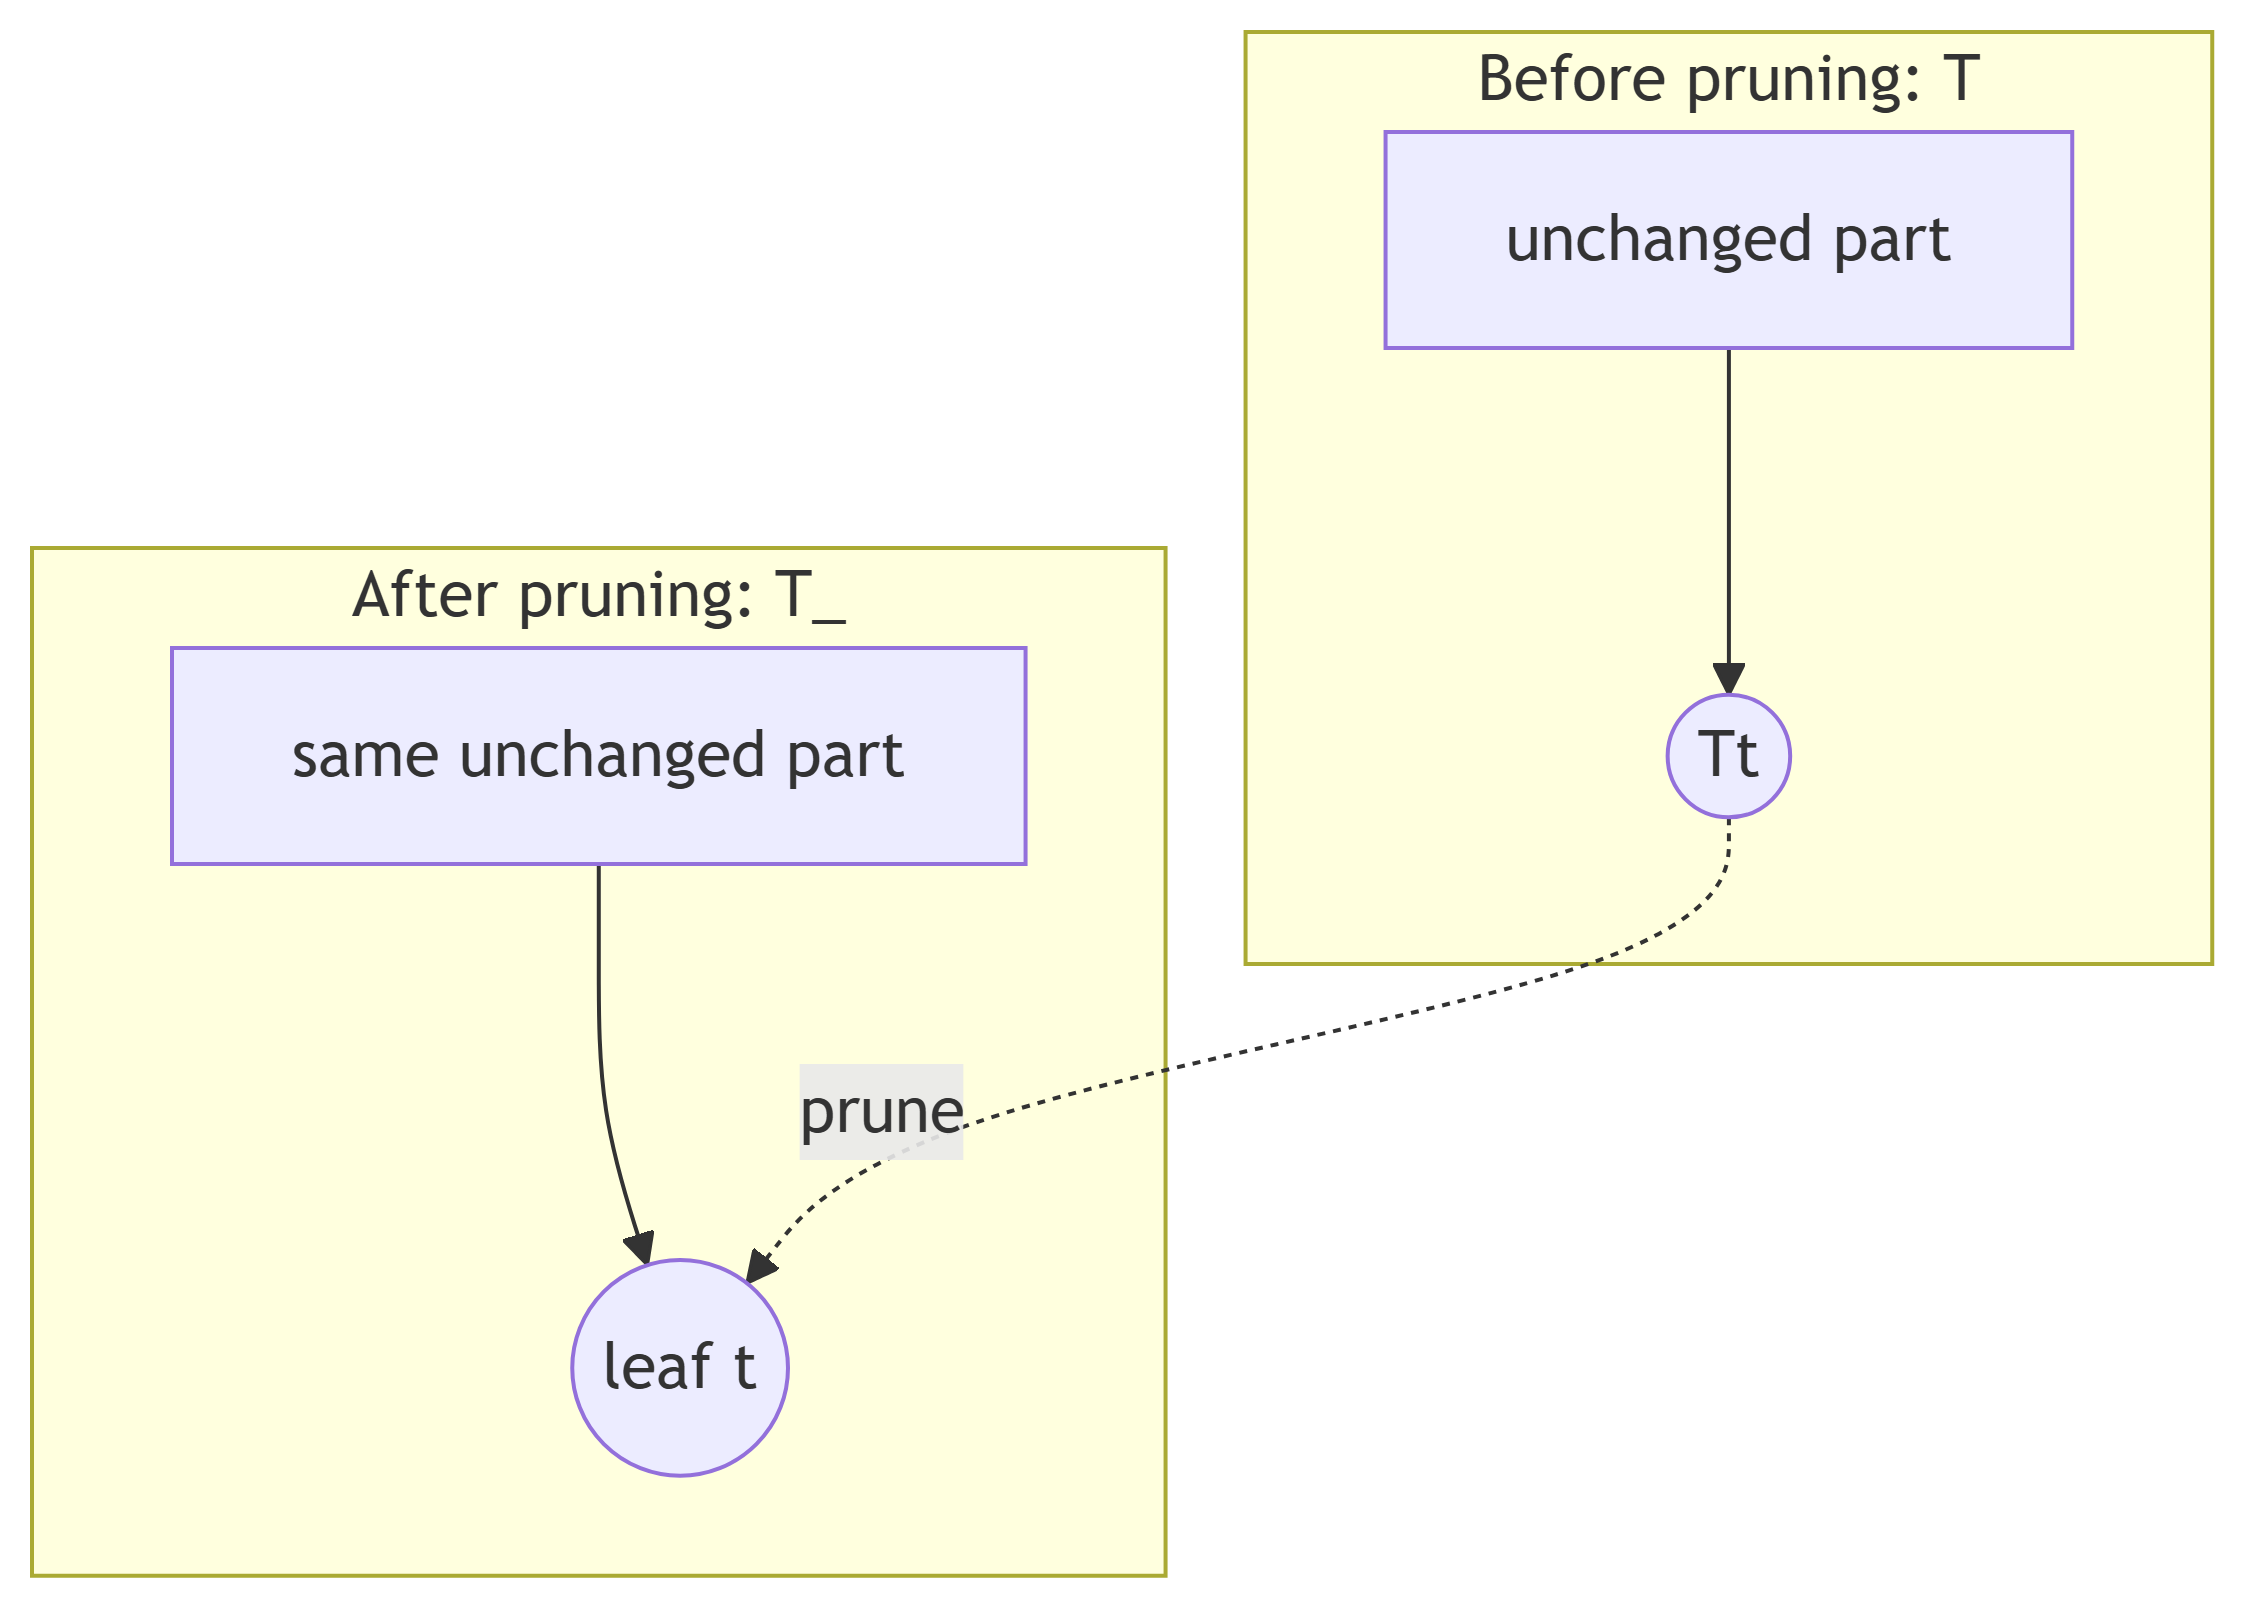
\includegraphics[width=5.84in,height=4.19in]{contents/2/tree_files/figure-latex/mermaid-figure-1.png}

The leaf \(t\) is already counted in \(T_-\). Expanding it into \(T_t\)
therefore adds \(|L(T_t)|-1\) leaves, so \[
|L(T)|-|L(T_-)|=|L(T_t)|-1.
\]

The reduction in cost from retaining \(T_t\) is \[
\begin{split}
C_{\alpha}(T_-)- C_{\alpha}(T)
&=\qty(J(T_-)+\alpha|L(T_-)|)-\qty(J(T)+\alpha|L(T)|)\\
&=\qty(J(T_-)-J(T))-\alpha(|L(T_t)|-1).
\end{split}
\] The subtree is worth retaining only when the cost is reduced
\(C_{\alpha}(T)<C_{\alpha}(T_-)\), which means that \[
J(T_-)-J(T)
>
\alpha\bigl(|L(T_t)|-1\bigr).
\]

Thus, the reduction in training cost must exceed the complexity penalty
for the additional leaves. When \(\alpha = 0\), there is no complexity
penalty, so the procedure behaves like an ordinary decision tree and
larger trees are generally preferred.

\end{example}

If the optimization problem were solved independently for each value of
\(\alpha\), there would be no obvious reason to expect the resulting
optimal subtrees to be related. However {[}7{]} proved that if
\(\alpha_1>\alpha_2\), then the optimal subtree for \(\alpha_1\) can
always be obtained by pruning subtrees from the optimal subtree for
\(\alpha_2\). Therefore, the MCCP algorithm views pruning as gradually
increasing \texttt{ccp\_alpha} from 0 to larger values, generating a
nested sequence of subtrees from the fully grown tree. The goal is to
find a tree that balances predictive performance and model complexity.

In practice, we first compute the \texttt{ccp\_alpha} path, which
contains the values of \texttt{ccp\_alpha} at which the optimal subtree
changes. We then use a validation set or cross-validation to evaluate
the subtrees along this path and select an appropriate value of
\texttt{ccp\_alpha}. If several candidate trees achieve similar
predictive performance, we usually prefer the simpler tree,
corresponding to a larger \texttt{ccp\_alpha}, because it is often more
stable and easier to interpret.

\subsection{Pre-pruning}\label{pre-pruning}

We often impose some early stopping conditions to limit the growth of a
tree. This strategy is called pre-pruning. Some common early stopping
conditions are:

\begin{itemize}
\tightlist
\item
  \texttt{max\_depth}: maximum tree depth
\item
  \texttt{min\_samples\_split}: minimum number of observations required
  to split a node
\item
  \texttt{min\_samples\_leaf}: minimum number of observations in a leaf
  node
\item
  \texttt{max\_leaf\_nodes}: maximum number of leaves
\end{itemize}

Smaller trees are usually more stable but may underfit. Larger trees are
more flexible but may overfit. A larger tree is not automatically
better, even if it achieves lower training error.

However, pre-pruning can be greedy. A split that appears only mildly
useful at an early stage may later enable highly informative splits
deeper in the tree. If we stop the tree too early, we may miss important
structure in the data.

Therefore, in modern practice, pre-pruning is usually not the primary
method for selecting the final model complexity. Instead, we mainly rely
on pruning by choosing the best \texttt{ccp\_alpha} through validation
or cross-validation. Pre-pruning is often used only as a guardrail to
prevent the initial tree from becoming excessively large. In practice,
we usually set relatively mild early stopping limits to stabilize the
tree-growing process and then rely on pruning to determine the final
tree size.

\begin{tcolorbox}[enhanced jigsaw, arc=.35mm, bottomrule=.15mm, bottomtitle=1mm, breakable, colback=white, colbacktitle=quarto-callout-note-color!10!white, colframe=quarto-callout-note-color-frame, coltitle=black, left=2mm, leftrule=.75mm, opacityback=0, opacitybacktitle=0.6, rightrule=.15mm, title=\textcolor{quarto-callout-note-color}{\faInfo}\hspace{0.5em}{Tuning in practice}, titlerule=0mm, toprule=.15mm, toptitle=1mm]

In classical CART, \texttt{ccp\_alpha} is the primary complexity
parameter and is usually selected by cross-validation after growing a
large tree.

In modern practice, pre-pruning parameters and \texttt{ccp\_alpha} are
often tuned together, especially for computational efficiency and
stability. In other words, methods such as \texttt{GridSearchCV} can be
used to tune all hyperparameters simultaneously.

However, when the search space becomes too large, this approach can
become computationally expensive. In that case, we often return to the
more traditional CART-style strategy: we first coarsely identify a
reasonable range for the early stopping hyperparameters and then
fine-tune \texttt{ccp\_alpha}.

\end{tcolorbox}

\section{Trees in Python}\label{trees-in-python}

We use \texttt{DecisionTreeClassifier} and
\texttt{DecisionTreeRegressor} from \texttt{sklearn.tree} to implement
decision tree models. The API is almost identical to other
\texttt{sklearn} models: \texttt{.fit()}, \texttt{.predict()},
\texttt{.score()}, and other familiar methods are used in the same way.

\begin{enumerate}
\def\labelenumi{\arabic{enumi}.}
\tightlist
\item
  We could set \texttt{max\_depth}, \texttt{min\_samples\_leaf},
  \texttt{ccp\_alpha}, etc. for the tree model where their meaning is
  straightforward.
\item
  The method \texttt{.cost\_complexity\_pruning\_path()} can be used to
  find the critical \texttt{ccp\_alpha} values for pruning.
\item
  We could also set \texttt{random\_state}. The randomness in
  \texttt{sklearn} decision trees mainly comes from the internal feature
  ordering used during the split search. Even when
  \texttt{splitter="best"} is used, \texttt{sklearn} randomly permutes
  the feature order before evaluating splits. Therefore, when multiple
  splits produce the same impurity reduction, different trees may be
  generated unless \texttt{random\_state} is fixed.
\end{enumerate}

\begin{tcolorbox}[enhanced jigsaw, arc=.35mm, bottomrule=.15mm, bottomtitle=1mm, breakable, colback=white, colbacktitle=quarto-callout-note-color!10!white, colframe=quarto-callout-note-color-frame, coltitle=black, left=2mm, leftrule=.75mm, opacityback=0, opacitybacktitle=0.6, rightrule=.15mm, title=\textcolor{quarto-callout-note-color}{\faInfo}\hspace{0.5em}{Note}, titlerule=0mm, toprule=.15mm, toptitle=1mm]

Decision trees are often described as methods that naturally handle
categorical predictors. This is true conceptually, but \texttt{sklearn}
decision trees still require numeric input. Therefore categorical
predictors must be encoded before fitting the model. For nominal
categorical variables, one-hot encoding is usually a safe choice.

However, one-hot encoding for the target variable is not necessary
because \texttt{sklearn} classifiers can directly work with class
labels.

\end{tcolorbox}

\subsection{\texorpdfstring{Example 1: Classify \texttt{iris}
dataset}{Example 1: Classify iris dataset}}\label{example-1-classify-iris-dataset}

The \texttt{iris} dataset is a classic classification dataset. The goal
is to use four numeric flower measurements to classify the species of
iris. The dataset contains 150 observations and 3 classes. More
information can be found in the \texttt{sklearn}
\hyperref[iris-datasetux29]{documentation} for datasets.

\begin{Shaded}
\begin{Highlighting}[]
\ImportTok{from}\NormalTok{ sklearn.datasets }\ImportTok{import}\NormalTok{ load\_iris}
\ImportTok{from}\NormalTok{ sklearn.model\_selection }\ImportTok{import}\NormalTok{ train\_test\_split}

\NormalTok{iris }\OperatorTok{=}\NormalTok{ load\_iris()}

\NormalTok{X }\OperatorTok{=}\NormalTok{ iris.data}
\NormalTok{y }\OperatorTok{=}\NormalTok{ iris.target}

\NormalTok{X\_train, X\_test, y\_train, y\_test }\OperatorTok{=}\NormalTok{ train\_test\_split(}
\NormalTok{    X, y, test\_size}\OperatorTok{=}\FloatTok{0.2}\NormalTok{, stratify}\OperatorTok{=}\NormalTok{y, random\_state}\OperatorTok{=}\DecValTok{1}
\NormalTok{)}
\end{Highlighting}
\end{Shaded}

The following code shows the basic \texttt{sklearn} API.

\begin{Shaded}
\begin{Highlighting}[]
\ImportTok{from}\NormalTok{ sklearn.tree }\ImportTok{import}\NormalTok{ DecisionTreeClassifier}

\NormalTok{clf }\OperatorTok{=}\NormalTok{ DecisionTreeClassifier(random\_state}\OperatorTok{=}\DecValTok{2}\NormalTok{)}
\NormalTok{clf.fit(X\_train, y\_train)}
\NormalTok{clf.score(X\_test, y\_test)}
\end{Highlighting}
\end{Shaded}

\begin{verbatim}
0.9666666666666667
\end{verbatim}

After fitting the model, we can display the tree using
\texttt{plot\_tree()}. In many real examples, the tree may be too large
to read clearly, so we use \texttt{matplotlib} to control the size and
resolution of the plot.

\protect\phantomsection\label{annotated-cell-175}%
\begin{Shaded}
\begin{Highlighting}[]
\ImportTok{from}\NormalTok{ sklearn.tree }\ImportTok{import}\NormalTok{ plot\_tree}
\ImportTok{import}\NormalTok{ matplotlib.pyplot }\ImportTok{as}\NormalTok{ plt}

\NormalTok{plt.figure(figsize}\OperatorTok{=}\NormalTok{(}\DecValTok{5}\NormalTok{, }\DecValTok{5}\NormalTok{), dpi}\OperatorTok{=}\DecValTok{300}\NormalTok{)}
\NormalTok{plot\_tree(clf, filled}\OperatorTok{=}\VariableTok{True}\NormalTok{, impurity}\OperatorTok{=}\VariableTok{True}\NormalTok{, node\_ids}\OperatorTok{=}\VariableTok{True}\NormalTok{)}\OperatorTok{;} \CommentTok{\# \textless{}1\textgreater{}}
\end{Highlighting}
\end{Shaded}

\begin{description}
\tightlist
\item[5CB6E08D-list-annote-1]
\texttt{filled=True} fills the nodes with colors. \texttt{impurity=Ture}
displays the Gini impurity. \texttt{node\_ids=True} displays the node
ID.
\end{description}

\pandocbounded{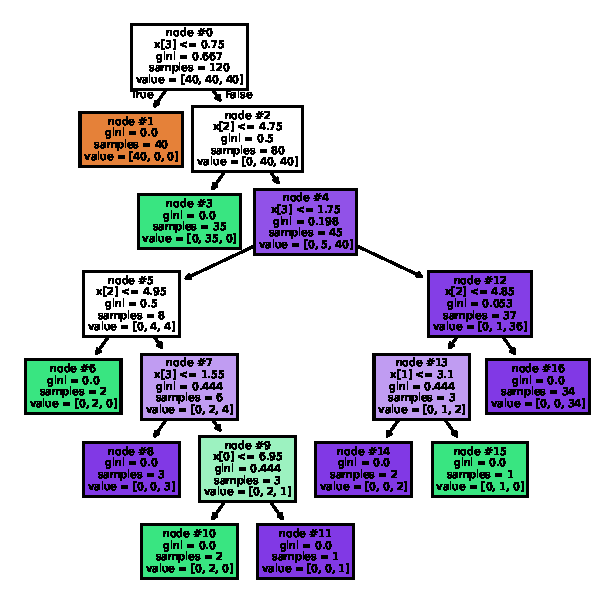
\includegraphics[keepaspectratio]{contents/2/tree_files/figure-pdf/cell-8-output-1.pdf}}

Now we prune the tree. We first find all critical \texttt{ccp\_alpha}
values.

\begin{Shaded}
\begin{Highlighting}[]
\NormalTok{ccp\_path }\OperatorTok{=}\NormalTok{ clf.cost\_complexity\_pruning\_path(X\_train, y\_train)}
\NormalTok{ccp\_alphas }\OperatorTok{=}\NormalTok{ ccp\_path.ccp\_alphas[:}\OperatorTok{{-}}\DecValTok{1}\NormalTok{]}
\end{Highlighting}
\end{Shaded}

The last \texttt{ccp\_alpha} is usually removed because it is large
enough to prune the tree down to a single root node. In most
applications, that model is too simple to be useful.

We then train one model for each effective \texttt{ccp\_alpha}. After
fitting the trees, we record both predictive performance and model
complexity. Here we use \texttt{accuracy} as our metric, which comes
automatically from \texttt{clf.score()}.

\begin{Shaded}
\begin{Highlighting}[]
\ImportTok{from}\NormalTok{ sklearn.metrics }\ImportTok{import}\NormalTok{ accuracy\_score}

\NormalTok{clfs }\OperatorTok{=}\NormalTok{ []}

\ControlFlowTok{for}\NormalTok{ ccp\_alpha }\KeywordTok{in}\NormalTok{ ccp\_alphas:}
\NormalTok{    clf }\OperatorTok{=}\NormalTok{ DecisionTreeClassifier(random\_state}\OperatorTok{=}\DecValTok{42}\NormalTok{, ccp\_alpha}\OperatorTok{=}\NormalTok{ccp\_alpha)}
\NormalTok{    clf.fit(X\_train, y\_train)}
\NormalTok{    clfs.append(clf)}

\NormalTok{node\_counts }\OperatorTok{=}\NormalTok{ [clf.tree\_.node\_count }\ControlFlowTok{for}\NormalTok{ clf }\KeywordTok{in}\NormalTok{ clfs]}
\NormalTok{train\_acc }\OperatorTok{=}\NormalTok{ [clf.score(X\_train, y\_train) }\ControlFlowTok{for}\NormalTok{ clf }\KeywordTok{in}\NormalTok{ clfs]}
\NormalTok{test\_acc }\OperatorTok{=}\NormalTok{ [clf.score(X\_test, y\_test) }\ControlFlowTok{for}\NormalTok{ clf }\KeywordTok{in}\NormalTok{ clfs]}
\end{Highlighting}
\end{Shaded}

Here we use a single train/test split for simplicity (by abusing
notations since we actually use test set as validation set). In addition
to accuracy, we also record the number of nodes because it is a useful
measure of tree complexity.

A larger tree usually has lower bias but higher variance. A smaller tree
is often more interpretable and more stable.

The results are easier to compare visually.

\protect\phantomsection\label{annotated-cell-178}%
\begin{Shaded}
\begin{Highlighting}[]
\ImportTok{import}\NormalTok{ matplotlib.pyplot }\ImportTok{as}\NormalTok{ plt}

\NormalTok{best\_alpha }\OperatorTok{=} \FloatTok{0.02}

\NormalTok{fig, ax }\OperatorTok{=}\NormalTok{ plt.subplots(}\DecValTok{2}\NormalTok{, }\DecValTok{1}\NormalTok{, figsize}\OperatorTok{=}\NormalTok{(}\DecValTok{7}\NormalTok{, }\DecValTok{7}\NormalTok{), sharex}\OperatorTok{=}\VariableTok{True}\NormalTok{)}

\NormalTok{ax[}\DecValTok{0}\NormalTok{].plot(ccp\_alphas, node\_counts, marker}\OperatorTok{=}\StringTok{"o"}\NormalTok{, drawstyle}\OperatorTok{=}\StringTok{"steps{-}post"}\NormalTok{) }\CommentTok{\# \textless{}1\textgreater{}}
\NormalTok{ax[}\DecValTok{1}\NormalTok{].plot(ccp\_alphas, train\_acc, marker}\OperatorTok{=}\StringTok{"o"}\NormalTok{, drawstyle}\OperatorTok{=}\StringTok{"steps{-}post"}\NormalTok{, label}\OperatorTok{=}\StringTok{"train"}\NormalTok{)}
\NormalTok{ax[}\DecValTok{1}\NormalTok{].plot(ccp\_alphas, test\_acc, marker}\OperatorTok{=}\StringTok{"o"}\NormalTok{, drawstyle}\OperatorTok{=}\StringTok{"steps{-}post"}\NormalTok{, label}\OperatorTok{=}\StringTok{"test"}\NormalTok{)}

\NormalTok{ax[}\DecValTok{0}\NormalTok{].axvline(best\_alpha, color}\OperatorTok{=}\StringTok{"black"}\NormalTok{, linestyle}\OperatorTok{=}\StringTok{"{-}{-}"}\NormalTok{, label}\OperatorTok{=}\StringTok{"best ccp\_alpha"}\NormalTok{)}
\NormalTok{ax[}\DecValTok{1}\NormalTok{].axvline(best\_alpha, color}\OperatorTok{=}\StringTok{"black"}\NormalTok{, linestyle}\OperatorTok{=}\StringTok{"{-}{-}"}\NormalTok{, label}\OperatorTok{=}\StringTok{"best ccp\_alpha"}\NormalTok{)}

\NormalTok{ax[}\DecValTok{1}\NormalTok{].set\_xlabel(}\StringTok{"ccp\_alpha"}\NormalTok{)}
\NormalTok{ax[}\DecValTok{0}\NormalTok{].set\_ylabel(}\StringTok{"number of nodes"}\NormalTok{)}
\NormalTok{ax[}\DecValTok{1}\NormalTok{].set\_ylabel(}\StringTok{"accuracy"}\NormalTok{)}

\NormalTok{ax[}\DecValTok{0}\NormalTok{].legend()}
\NormalTok{ax[}\DecValTok{1}\NormalTok{].legend(loc}\OperatorTok{=}\StringTok{"lower left"}\NormalTok{)}
\end{Highlighting}
\end{Shaded}

\begin{description}
\tightlist
\item[5CB6E08D-list-annote-1]
For pruning-related plots, \texttt{drawstyle="steps-post"} is important
because the tree structure stays the same within each interval of
\texttt{ccp\_alpha} values. The tree only changes after reaching the
next pruning threshold. Each critical \texttt{ccp\_alpha} corresponds to
pruning one or more weak internal nodes, so the pruning path is
piecewise constant.
\end{description}

\pandocbounded{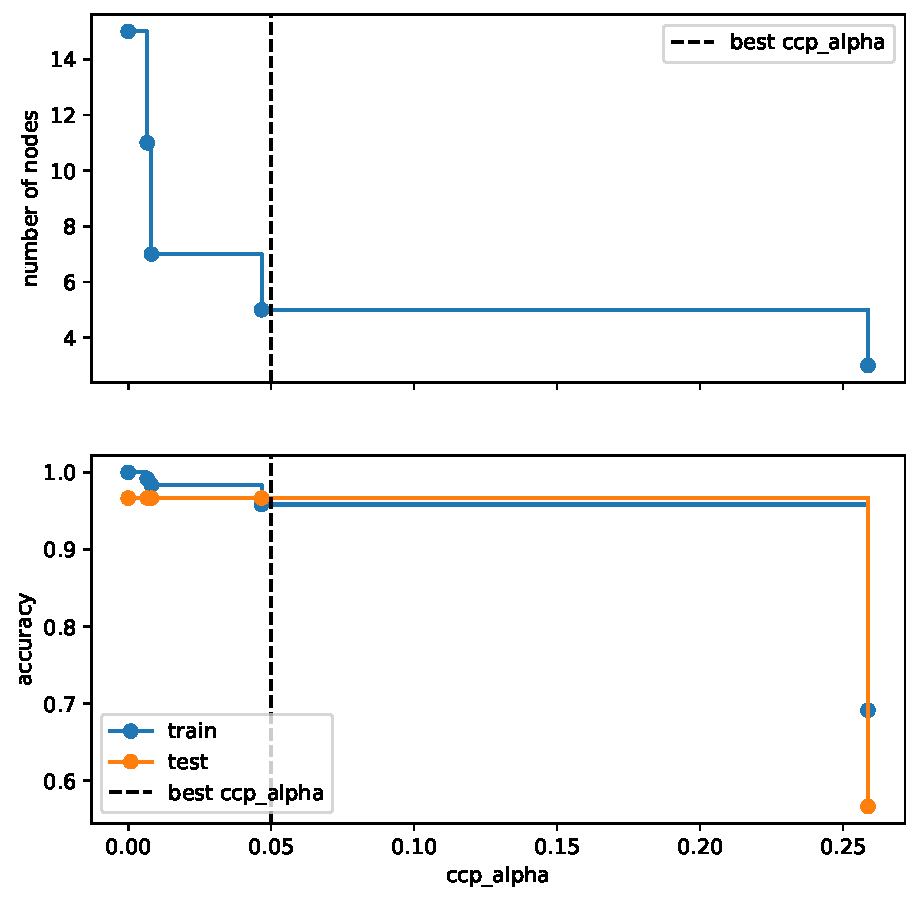
\includegraphics[keepaspectratio]{contents/2/tree_files/figure-pdf/cell-11-output-1.pdf}}

Based on the plot, from 0.0 \(\leq\) \texttt{ccp\_alpha} \(<\)
0.02452452452452452, the test accuracy stay the same. Therefore we would
like to choose the one with the least number of nodes, which is
0.011111111111111113. Since all \(\alpha\) values in the range give the
same tree, we hand pick \texttt{ccp\_alpha=0.02} for simplicity.

We can now build the final tree and display it.

\begin{Shaded}
\begin{Highlighting}[]
\NormalTok{clf }\OperatorTok{=}\NormalTok{ DecisionTreeClassifier(random\_state}\OperatorTok{=}\DecValTok{42}\NormalTok{, ccp\_alpha}\OperatorTok{=}\NormalTok{best\_alpha)}
\NormalTok{clf.fit(X\_train, y\_train)}
\NormalTok{plot\_tree(clf, filled}\OperatorTok{=}\VariableTok{True}\NormalTok{, impurity}\OperatorTok{=}\VariableTok{True}\NormalTok{, node\_ids}\OperatorTok{=}\VariableTok{True}\NormalTok{)}\OperatorTok{;}
\end{Highlighting}
\end{Shaded}

\pandocbounded{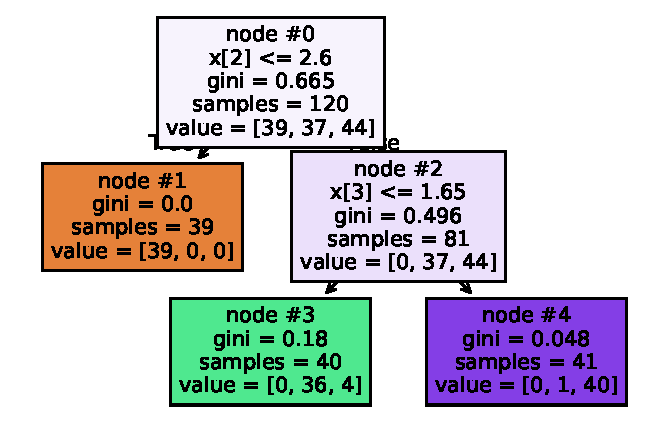
\includegraphics[keepaspectratio]{contents/2/tree_files/figure-pdf/cell-12-output-1.pdf}}

\begin{tcolorbox}[enhanced jigsaw, arc=.35mm, bottomrule=.15mm, bottomtitle=1mm, breakable, colback=white, colbacktitle=quarto-callout-note-color!10!white, colframe=quarto-callout-note-color-frame, coltitle=black, left=2mm, leftrule=.75mm, opacityback=0, opacitybacktitle=0.6, rightrule=.15mm, title=\textcolor{quarto-callout-note-color}{\faInfo}\hspace{0.5em}{Note}, titlerule=0mm, toprule=.15mm, toptitle=1mm]

Although the hyperparameters with the highest validation score are often
preferred, model complexity should also be taken into consideration.
This is why the number of nodes is displayed.

In this \texttt{iris} example, the dataset is very small and the
differences between validation scores are negligible. In such
situations, a slightly simpler tree is often preferred because it is
more interpretable and potentially more stable while achieving similar
predictive performance.

In larger datasets, small differences in validation scores are often
more meaningful, so predictive performance may be prioritized more
heavily.

\end{tcolorbox}

\subsection{\texorpdfstring{Example 2: Regression with the
\texttt{diabetes}
dataset}{Example 2: Regression with the diabetes dataset}}\label{example-2-regression-with-the-diabetes-dataset}

We now look at a regression example. The \texttt{diabetes} dataset uses
10 baseline variables to predict a quantitative measure of disease
progression one year after baseline. More information can be found in
the \texttt{sklearn} \hyperref[diabetes-datasetux29]{documentation} and
the original diabetes dataset
\href{(https://www4.stat.ncsu.edu/~boos/var.select/diabetes.html)}{description}.

\begin{Shaded}
\begin{Highlighting}[]
\ImportTok{from}\NormalTok{ sklearn.datasets }\ImportTok{import}\NormalTok{ load\_diabetes}
\ImportTok{from}\NormalTok{ sklearn.model\_selection }\ImportTok{import}\NormalTok{ train\_test\_split}

\NormalTok{X, y }\OperatorTok{=}\NormalTok{ load\_diabetes(return\_X\_y}\OperatorTok{=}\VariableTok{True}\NormalTok{)}
\NormalTok{X\_train, X\_test, y\_train, y\_test }\OperatorTok{=}\NormalTok{ train\_test\_split(X, y, test\_size}\OperatorTok{=}\FloatTok{0.2}\NormalTok{, random\_state}\OperatorTok{=}\DecValTok{1}\NormalTok{)}
\end{Highlighting}
\end{Shaded}

The overall workflow is similar to the \texttt{iris} example. In this
example, we choose to use cross-validation instead of a single
validation split in order to obtain a more stable estimate of model
performance. This is not specific to regression trees; either approach
can be used for both classification and regression problems.

We first create a temporary tree to compute the critical
\texttt{ccp\_alpha} values. The method
\texttt{cost\_complexity\_pruning\_path()} internally grows a tree in
order to compute the effective pruning path, although the estimator
itself is not stored as a fitted model.

\begin{Shaded}
\begin{Highlighting}[]
\ImportTok{from}\NormalTok{ sklearn.tree }\ImportTok{import}\NormalTok{ DecisionTreeRegressor}

\NormalTok{base\_tree }\OperatorTok{=}\NormalTok{ DecisionTreeRegressor(random\_state}\OperatorTok{=}\DecValTok{1}\NormalTok{)}
\NormalTok{path }\OperatorTok{=}\NormalTok{ base\_tree.cost\_complexity\_pruning\_path(X\_train, y\_train)}
\NormalTok{ccp\_alphas }\OperatorTok{=}\NormalTok{ path.ccp\_alphas[:}\OperatorTok{{-}}\DecValTok{1}\NormalTok{]}
\end{Highlighting}
\end{Shaded}

This follows the classical CART pruning strategy:

\begin{enumerate}
\def\labelenumi{\arabic{enumi}.}
\tightlist
\item
  Grow a large tree.
\item
  Compute the pruning path.
\item
  Use validation or cross-validation to select the final subtree.
\end{enumerate}

Now we run \texttt{GridSearchCV} over these \texttt{ccp\_alpha} values.
We use \(R^2\) as the model metric in this example.

\begin{Shaded}
\begin{Highlighting}[]
\ImportTok{from}\NormalTok{ sklearn.model\_selection }\ImportTok{import}\NormalTok{ GridSearchCV}
\ImportTok{from}\NormalTok{ sklearn.metrics }\ImportTok{import}\NormalTok{ r2\_score}

\NormalTok{params }\OperatorTok{=}\NormalTok{ param\_grid }\OperatorTok{=}\NormalTok{ \{}\StringTok{"ccp\_alpha"}\NormalTok{: ccp\_alphas\}}
\NormalTok{grid }\OperatorTok{=}\NormalTok{ GridSearchCV(}
\NormalTok{    DecisionTreeRegressor(random\_state}\OperatorTok{=}\DecValTok{1}\NormalTok{), param\_grid}\OperatorTok{=}\NormalTok{params, scoring}\OperatorTok{=}\StringTok{"r2"}
\NormalTok{)}

\NormalTok{grid.fit(X\_train, y\_train)}

\NormalTok{best\_tree }\OperatorTok{=}\NormalTok{ grid.best\_estimator\_}

\NormalTok{y\_pred\_train }\OperatorTok{=}\NormalTok{ best\_tree.predict(X\_train)}
\NormalTok{y\_pred\_test }\OperatorTok{=}\NormalTok{ best\_tree.predict(X\_test)}

\BuiltInTok{print}\NormalTok{(}\SpecialStringTok{f"Best ccp\_alpha: }\SpecialCharTok{\{}\NormalTok{grid}\SpecialCharTok{.}\NormalTok{best\_params\_[}\StringTok{\textquotesingle{}ccp\_alpha\textquotesingle{}}\NormalTok{]}\SpecialCharTok{\}}\SpecialStringTok{"}\NormalTok{)}
\BuiltInTok{print}\NormalTok{(}\SpecialStringTok{f"Training R\^{}2: }\SpecialCharTok{\{}\NormalTok{r2\_score(y\_train, y\_pred\_train)}\SpecialCharTok{\}}\SpecialStringTok{"}\NormalTok{)}
\BuiltInTok{print}\NormalTok{(}\SpecialStringTok{f"Testing R\^{}2: }\SpecialCharTok{\{}\NormalTok{r2\_score(y\_test, y\_pred\_test)}\SpecialCharTok{\}}\SpecialStringTok{"}\NormalTok{)}
\end{Highlighting}
\end{Shaded}

\begin{verbatim}
Best ccp_alpha: 105.18472145590351
Training R^2: 0.5347863093947497
Testing R^2: 0.1922738375305083
\end{verbatim}

We can visualize the cross-validation curve. \texttt{GridSearchCV}
records validation scores, but it does not automatically record tree
complexity measures such as the number of nodes. Therefore, if we want
to display the complexity curve, we need to refit the models for the
same \texttt{ccp\_alpha} values and record their node counts.

\begin{Shaded}
\begin{Highlighting}[]
\NormalTok{cv\_score }\OperatorTok{=}\NormalTok{ grid.cv\_results\_[}\StringTok{"mean\_test\_score"}\NormalTok{]}

\NormalTok{node\_counts }\OperatorTok{=}\NormalTok{ []}
\ControlFlowTok{for}\NormalTok{ ccp\_alpha }\KeywordTok{in}\NormalTok{ ccp\_alphas:}
\NormalTok{    tree }\OperatorTok{=}\NormalTok{ DecisionTreeRegressor(random\_state}\OperatorTok{=}\DecValTok{1}\NormalTok{, ccp\_alpha}\OperatorTok{=}\NormalTok{ccp\_alpha)}
\NormalTok{    tree.fit(X\_train, y\_train)}
\NormalTok{    node\_counts.append(tree.tree\_.node\_count)}

\NormalTok{best\_alpha }\OperatorTok{=}\NormalTok{ grid.best\_params\_[}\StringTok{"ccp\_alpha"}\NormalTok{]}

\NormalTok{fig, ax }\OperatorTok{=}\NormalTok{ plt.subplots(}\DecValTok{2}\NormalTok{, }\DecValTok{1}\NormalTok{, figsize}\OperatorTok{=}\NormalTok{(}\DecValTok{7}\NormalTok{, }\DecValTok{7}\NormalTok{), sharex}\OperatorTok{=}\VariableTok{True}\NormalTok{)}

\NormalTok{ax[}\DecValTok{0}\NormalTok{].plot(ccp\_alphas, node\_counts, marker}\OperatorTok{=}\StringTok{"o"}\NormalTok{, drawstyle}\OperatorTok{=}\StringTok{"steps{-}post"}\NormalTok{)}
\NormalTok{ax[}\DecValTok{1}\NormalTok{].plot(ccp\_alphas, cv\_score, marker}\OperatorTok{=}\StringTok{"o"}\NormalTok{, drawstyle}\OperatorTok{=}\StringTok{"steps{-}post"}\NormalTok{, label}\OperatorTok{=}\StringTok{"CV score"}\NormalTok{)}

\NormalTok{ax[}\DecValTok{0}\NormalTok{].axvline(best\_alpha, color}\OperatorTok{=}\StringTok{"black"}\NormalTok{, linestyle}\OperatorTok{=}\StringTok{"{-}{-}"}\NormalTok{, label}\OperatorTok{=}\StringTok{"best ccp\_alpha"}\NormalTok{)}
\NormalTok{ax[}\DecValTok{1}\NormalTok{].axvline(best\_alpha, color}\OperatorTok{=}\StringTok{"black"}\NormalTok{, linestyle}\OperatorTok{=}\StringTok{"{-}{-}"}\NormalTok{, label}\OperatorTok{=}\StringTok{"best ccp\_alpha"}\NormalTok{)}

\NormalTok{ax[}\DecValTok{1}\NormalTok{].set\_xlabel(}\StringTok{"ccp\_alpha"}\NormalTok{)}
\NormalTok{ax[}\DecValTok{0}\NormalTok{].set\_ylabel(}\StringTok{"number of nodes"}\NormalTok{)}
\NormalTok{ax[}\DecValTok{1}\NormalTok{].set\_ylabel(}\StringTok{"CV $R\^{}2$"}\NormalTok{)}

\NormalTok{ax[}\DecValTok{0}\NormalTok{].legend()}
\NormalTok{ax[}\DecValTok{1}\NormalTok{].legend(loc}\OperatorTok{=}\StringTok{"lower left"}\NormalTok{)}
\end{Highlighting}
\end{Shaded}

\pandocbounded{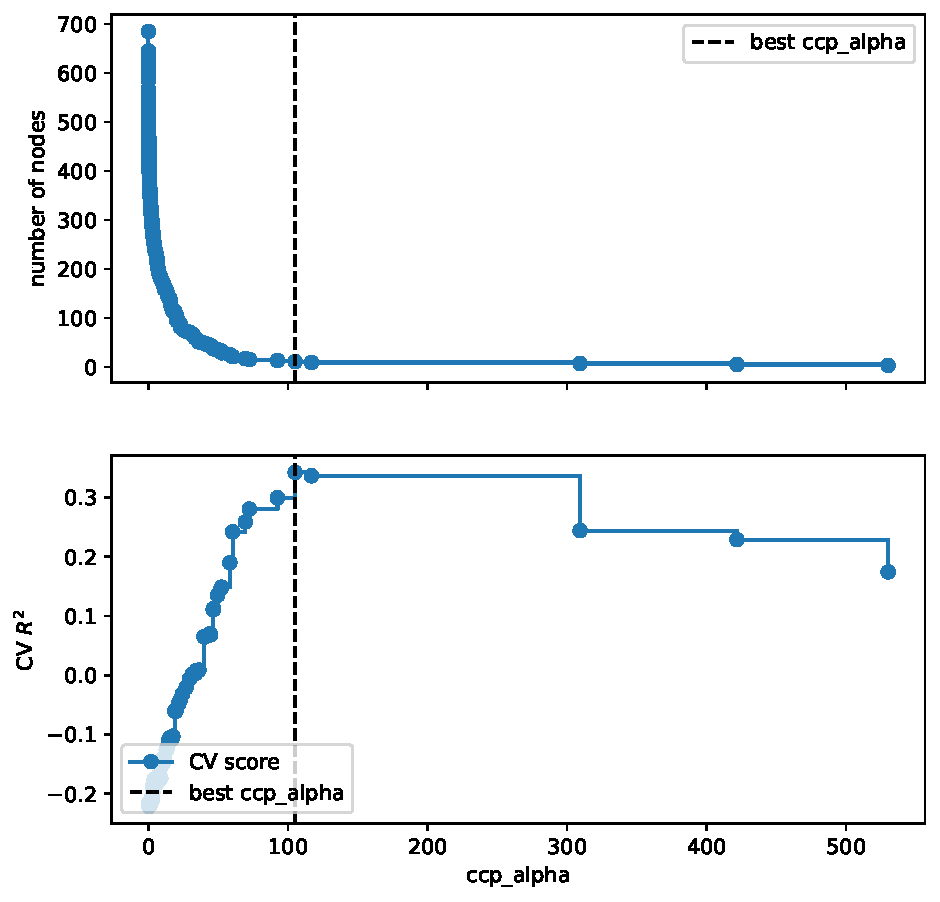
\includegraphics[keepaspectratio]{contents/2/tree_files/figure-pdf/cell-16-output-1.pdf}}

From the plot, our selected
\texttt{ccp\_alpha}=np.float64(105.18472145590351) is reasonable since
it gives a relative strong cross-validation score without producing an
unnecessarily large tree.

\begin{tcolorbox}[enhanced jigsaw, arc=.35mm, bottomrule=.15mm, bottomtitle=1mm, breakable, colback=white, colbacktitle=quarto-callout-warning-color!10!white, colframe=quarto-callout-warning-color-frame, coltitle=black, left=2mm, leftrule=.75mm, opacityback=0, opacitybacktitle=0.6, rightrule=.15mm, title=\textcolor{quarto-callout-warning-color}{\faExclamationTriangle}\hspace{0.5em}{Warning}, titlerule=0mm, toprule=.15mm, toptitle=1mm]

A single regression tree often has unstable predictive performance on
moderate-sized noisy datasets. Therefore, the test \(R^2\) may not look
high in this example. This is one reason why ensemble methods such as
random forests and boosting are often preferred in practice.

\end{tcolorbox}

\chapter{Bagging and Random Forests}\label{bagging-and-random-forests}

In earlier chapters we studied single decision trees. A tree is flexible
because it can capture nonlinear relationships and interactions without
specifying them in advance. However, a single tree is also unstable. A
small change in the training data may produce a very different tree,
especially when the tree is grown deeply.

Bagging and random forests are ensemble methods designed to reduce this
instability.

The central idea is:

\begin{quote}
Instead of trusting one unstable tree, build many unstable trees and
average them.
\end{quote}

This chapter first discusses bagging. Random forests will then be
introduced as an improvement of bagging. Since bagging and random
forests use almost the same aggregation idea for regression and
classification, we will mainly use regression notation. For
classification, averages are usually replaced by majority vote or
averaged class probabilities.

\section{Ensemble Averaging}\label{ensemble-averaging}

Suppose we observe training data

\[
\{(x_i,y_i)\}_{i=1}^n,
\quad x_i\in\mathbb R^p,
\quad y_i\in\mathbb R.
\]

An ensemble combines many fitted models

\[
\hat f_1,\hat f_2,\ldots,\hat f_B
\]

into one final predictor. For regression, the simplest ensemble average
is

\[
\hat f_{\text{ens}}(x)
=
\frac1B\sum_{b=1}^B \hat f_b(x).
\]

Each individual model may be noisy. However, the average can be much
more stable.

To see why, suppose each \(\hat f_b(x)\) has variance \(\sigma^2\), and
suppose for a moment that the fitted models are independent. Then

\[
\Var\left(
\frac1B\sum_{b=1}^B \hat f_b(x)
\right)
=
\frac{\sigma^2}{B}.
\]

Thus averaging can greatly reduce variance.

In practice, the fitted models are not independent. If the pairwise
correlation between two fitted models is approximately \(\rho\), then

Click to expand.

\[
\cor(\hat f_i(x),\hat f_j(x))\approx \rho, \qquad i\ne j.
\]

Then

\[
\Cov(\hat f_i(x),\hat f_j(x))
=
\cor(\hat f_i(x),\hat f_j(x))
\sqrt{\Var(\hat f_i(x))\Var(\hat f_j(x))}
\approx
\rho\sigma^2.
\]

Therefore,

\[
\begin{aligned}
\Var\left(
\frac1B\sum_{b=1}^B \hat f_b(x)
\right)
&=
\frac1{B^2}
\left[
\sum_{b=1}^B \Var(\hat f_b(x))
+
\sum_{i\ne j}\Cov(\hat f_i(x),\hat f_j(x))
\right] \\[4pt]
&\approx
\frac1{B^2}
\left[
B\sigma^2
+
B(B-1)\rho\sigma^2
\right] \\[4pt]
&=
\sigma^2
\left[
\frac1B+\frac{B-1}{B}\rho
\right] \\[4pt]
&=
\rho\sigma^2+\frac{1-\rho}{B}\sigma^2.
\end{aligned}
\]

Then

\[
\Var\left(
\frac1B\sum_{b=1}^B \hat f_b(x)
\right)
\approx
\rho\sigma^2
+
\frac{1-\rho}{B}\sigma^2.
\]

This formula is very important. Increasing \(B\) reduces the second
term, but the first term remains. Therefore, if the individual trees are
highly correlated, averaging has limited benefit.

\section{Bagging}\label{bagging}

Bagging is short for bootstrap aggregation.

Assume the original training set has \(n\) data. A bootstrap sample is a
sample drawn from the original training data with replacement. Each
bootstrap sample has size \(n\), but because sampling is done with
replacement, some observations appear more than once and some
observations do not appear at all.

Let \(Z=\{(x_1,y_1),\ldots,(x_n,y_n)\}\) be the original training set.
Bagging constructs bootstrap samples \(Z^{*1},Z^{*2},\ldots,Z^{*B}\).
For each bootstrap sample \(Z^{*b}\), we fit a model \(\hat f_b(x)\).
The bagged regression estimate is then

\[
\hat f_{\text{bag}}(x)
=
\frac1B\sum_{b=1}^B \hat f_b(x).
\]

For classification, the final prediction is usually based on majority
vote:

\[
\hat G_{\text{bag}}(x)
=
\Mode\{\hat G_1(x),\ldots,\hat G_B(x)\}.
\]

Equivalently, we may average estimated class probabilities and choose
the class with the largest average probability.

\begin{tcolorbox}[enhanced jigsaw, arc=.35mm, bottomrule=.15mm, bottomtitle=1mm, breakable, colback=white, colbacktitle=quarto-callout-note-color!10!white, colframe=quarto-callout-note-color-frame, coltitle=black, left=2mm, leftrule=.75mm, opacityback=0, opacitybacktitle=0.6, rightrule=.15mm, title=\textcolor{quarto-callout-note-color}{\faInfo}\hspace{0.5em}{Bias-variance view}, titlerule=0mm, toprule=.15mm, toptitle=1mm]

Bagging is useful when the base learner is unstable. A decision tree is
a typical unstable learner. Different bootstrap samples lead to
different trees, because each tree sees a slightly different version of
the data.

For a decision tree, bagging usually uses large trees rather than
heavily pruned trees. The reason is that a large tree has low bias but
high variance. Bagging is designed to reduce variance, so it is natural
to start with a flexible base learner.

A single deep tree usually has low bias and high variance. Bagging keeps
the low bias and reduces the variance by averaging many deep trees.

\end{tcolorbox}

\begin{tcolorbox}[enhanced jigsaw, arc=.35mm, bottomrule=.15mm, bottomtitle=1mm, breakable, colback=white, colbacktitle=quarto-callout-caution-color!10!white, colframe=quarto-callout-caution-color-frame, coltitle=black, left=2mm, leftrule=.75mm, opacityback=0, opacitybacktitle=0.6, rightrule=.15mm, title=\textcolor{quarto-callout-caution-color}{\faFire}\hspace{0.5em}{Bagging estimators}, titlerule=0mm, toprule=.15mm, toptitle=1mm]

Although bagging is most commonly applied to decision trees, it can also
be used with other types of models.

\end{tcolorbox}

\subsection{Out-of-Bag Error}\label{out-of-bag-error}

Although a bootstrap sample has size \(n\), it does not contain all
\(n\) observations.

\begin{definition}[Out-of-bag
observations]\protect\hypertarget{def-}{}\label{def-}

Each bootstrap sample contains about \(63.2\%\) of the original
observations as distinct observations. The remaining observations are
called \textbf{out-of-bag} (OOB) observations for that bootstrap sample.

Click to expand.

For a fixed observation \(i\), the probability that it is not selected
in one draw is

\[
1-\frac1n.
\]

The probability that it is never selected in \(n\) draws is

\[
\left(1-\frac1n\right)^n.
\]

When \(n\) is large,

\[
\left(1-\frac1n\right)^n
\to
e^{-1}
\approx
0.368.
\]

Therefore, the probability that observation \(i\) appears at least once
is approximately

\[
1-e^{-1}
\approx
0.632,
\] and it is the expected proportion of distinct observations in a
sample.

\end{definition}

The OOB observations give a natural way to estimate prediction error.

For observation \(i\), consider only the trees for which observation
\(i\) was out-of-bag. Average those trees to get an OOB prediction:

\[
\hat f_{\text{OOB},i}
=
\frac{1}{|B_i|}
\sum_{b\in B_i}\hat f_b(x_i),
\]

where \(B_i\) is the set of trees that did not use observation \(i\) in
their bootstrap sample.

The OOB mean squared error is

\[
\operatorname{MSE}_{\text{OOB}}
=
\frac1n
\sum_{i=1}^n
\left(y_i-\hat f_{\text{OOB},i}\right)^2.
\]

All other metrics have OOB versions in the straightforward way.

OOB error is useful because it behaves like an internal validation
estimate. We do not need to set aside a separate validation set just to
estimate the error of the bagged model. Therefore, for bagging, in
addition to single-split validation and cross-validation, we can also
use OOB validation to tune hyperparameters.

\section{Random Forests}\label{random-forests}

Random forests are a modification of bagging for decision trees. In
addition to the diversity by sampling observations from Bagging, Random
forests create additional diversity by sampling features during tree
construction.

The random forest algorithm for regression is:

\begin{enumerate}
\def\labelenumi{\arabic{enumi}.}
\tightlist
\item
  Draw a bootstrap sample from the training data.
\item
  Grow a large regression tree on this bootstrap sample.
\item
  \textbf{At each split, randomly choose \(m\) predictors from the full
  set of \(p\) predictors.}
\item
  \textbf{Find the best split only among those \(m\) predictors.}
\item
  Repeat this process for \(B\) trees.
\item
  Average the predictions.
\end{enumerate}

The final random forest regressor is

\[
\hat f_{\text{RF}}(x)
=
\frac1B\sum_{b=1}^B\hat f_b(x).
\]

The formula looks the same as bagging. The difference is how the trees
are grown.

The key difference from Bagging(Trees) is the Step 3 and 4. In ordinary
bagging, all predictors are available at every split. If there is one
very strong predictor, many trees may split on that same predictor near
the top of the tree. As a result, the trees become similar.

Similar trees are highly correlated. From the variance formula,

\[
\rho\sigma^2
+
\frac{1-\rho}{B}\sigma^2,
\]

we know that high correlation limits the benefit of averaging.

Now random forests reduce this issue by forcing each split to consider
only a random subset of predictors. This prevents the strongest
predictors from dominating every tree. The trees become less correlated,
and averaging becomes more effective.

\subsection{\texorpdfstring{\texttt{max\_features}}{max\_features}}\label{max_features}

How many predictors are considered at each split? In \texttt{sklearn},
this is controlled by \texttt{max\_features}. This is a very important
hyperparameter because it affects the correlations between trees.

Large \texttt{max\_features} means each tree can choose from many
predictors. Individual trees may become stronger, but the trees may also
become more similar to each other.

Small \texttt{max\_features} forces trees to explore different
predictors. This usually decreases the correlations between trees, but
each individual tree may become weaker.

Thus \texttt{max\_features} controls an important tradeoff between tree
strength and tree correlation.

Common traditional choices are:

\begin{itemize}
\tightlist
\item
  for classification, \texttt{max\_features}\(=\sqrt p\)
\item
  for regression, \texttt{max\_features}\(=p/3\)
\end{itemize}

These recommendations originated from the original Random Forest
literature {[}8{]} and later became popular defaults in many software
implementations {[}3{]}. They are mainly based on empirical experience
and the general intuition that:

\begin{itemize}
\tightlist
\item
  classification forests often benefit more from tree diversity
\item
  regression forests often benefit more from stronger individual trees
\end{itemize}

In modern practice, however, \texttt{max\_features} is usually treated
as a tuning hyperparameter and is commonly selected using validation or
cross-validation.

\subsection{Random Forest as Adaptive Local
Averaging}\label{random-forest-as-adaptive-local-averaging}

A random forest can also be viewed as a data-adaptive local averaging
method.

For one tree, two points are close if they fall in the same terminal
node. Let

\[
I_b(x,x_i)
=
\begin{cases}1,&\text{ if $x$ and $x_i$ are in the same leaf of tree $b$},\\
0,&\text{ otherwise}.
\end{cases}
\]

Across the whole forest, define the similarity

\[
K_{\text{RF}}(x,x_i)
=
\frac{1}{B}\sum_{b=1}^B I_b(x,x_i).
\]

This measures the proportion of trees in which \(x\) and \(x_i\) fall
into the same terminal node. The quantity \(K_{\text{RF}}(x,x_i)\) can
be interpreted as a data-adaptive similarity measure between \(x\) and
\(x_i\).

The random forest prediction can be written as a weighted average

\[
\hat f_{\text{RF}}(x)
=
\sum_{i=1}^n w_i(x)y_i,
\]

where observations that frequently share terminal nodes with \(x\)
receive larger weights.

More details about the adaptive nearest-neighbor interpretation of
random forests can be found in {[}9{]} and {[}3{]}.

\begin{tcolorbox}[enhanced jigsaw, arc=.35mm, bottomrule=.15mm, bottomtitle=1mm, breakable, colback=white, colbacktitle=quarto-callout-note-color!10!white, colframe=quarto-callout-note-color-frame, coltitle=black, left=2mm, leftrule=.75mm, opacityback=0, opacitybacktitle=0.6, rightrule=.15mm, title=\textcolor{quarto-callout-note-color}{\faInfo}\hspace{0.5em}{Note}, titlerule=0mm, toprule=.15mm, toptitle=1mm]

The adaptive-neighbor interpretation helps explain why random forests
often perform much better than classical distance-based methods such as
KNN in complex datasets.

In KNN, neighborhoods are determined by a fixed geometric distance. In
contrast, random forests learn the neighborhood structure directly from
the data through recursive splitting. Two observations are considered
close if the forest repeatedly places them into the same terminal nodes,
so the similarity automatically adapts to the importance of variables
and their relationships with the response variable.

As a result, the neighborhood automatically adapts to:

\begin{itemize}
\tightlist
\item
  important variables
\item
  interaction effects
\item
  nonlinear structures
\item
  local heterogeneity of the feature space
\end{itemize}

This viewpoint also provides intuition for why random forests are often
robust in high-dimensional settings. Instead of relying on a global
distance metric, the forest constructs many local data-dependent
neighborhoods and averages over them.

From a theoretical perspective, this interpretation connects random
forests to classical nonparametric smoothing methods such as KNN and
kernel regression, helping explain random forests using the broader
language of statistical learning theory.

\end{tcolorbox}

\subsection{Feature Importance}\label{feature-importance}

There are two commonly used measures of feature importance. We briefly
discuss them here. More detailed examples and implementations can be
found in the
\href{https://scikit-learn.org/stable/auto_examples/inspection/plot_permutation_importance.html}{scikit-learn
documentation}.

\subsubsection{Mean Decrease in
Impurity}\label{mean-decrease-in-impurity}

One common measure is impurity-based importance, also called Mean
Decrease in Impurity (MDI). This importance measure is specific to
tree-based methods because it depends directly on the tree splitting
process.

Recall that when building a tree, each split is selected to reduce a
splitting impurity (or loss), such as:

\begin{itemize}
\tightlist
\item
  squared error for regression
\item
  Gini impurity for classification
\end{itemize}

Impurity-based importance measures how much a variable decreases the
splitting impurity across all splits in all trees. Variables that
frequently produce large impurity reductions receive larger importance
values.

For a single tree, the feature importance is simply the total impurity
reduction contributed by that variable across all splits in the tree.
However, because a single decision tree is often unstable and has high
variance, these importance values may vary substantially from one tree
to another. In bagging and Random Forests, the importance values are
averaged across many trees, producing a much more stable and reliable
measure of variable importance.

\subsubsection{Permutation importance}\label{permutation-importance}

Another common measure is permutation importance. Unlike impurity-based
importance, permutation importance is a general model-agnostic method
and is not specific to trees or Random Forests.

The basic idea is:

\begin{enumerate}
\def\labelenumi{\arabic{enumi}.}
\tightlist
\item
  Measure prediction error on validation data.
\item
  Randomly permute one predictor.
\item
  Measure prediction error again.
\end{enumerate}

Permuting a predictor destroys the relationship between that predictor
and the response while keeping the marginal distribution unchanged. If
permuting a predictor substantially worsens predictive performance, then
the model strongly relies on that predictor, indicating high importance.

Permutation importance is often easier to interpret because it is
directly tied to predictive performance rather than the internal
structure of the model.

\begin{tcolorbox}[enhanced jigsaw, arc=.35mm, bottomrule=.15mm, bottomtitle=1mm, breakable, colback=white, colbacktitle=quarto-callout-note-color!10!white, colframe=quarto-callout-note-color-frame, coltitle=black, left=2mm, leftrule=.75mm, opacityback=0, opacitybacktitle=0.6, rightrule=.15mm, title=\textcolor{quarto-callout-note-color}{\faInfo}\hspace{0.5em}{MDI vs Permutation Importance}, titlerule=0mm, toprule=.15mm, toptitle=1mm]

The two methods answer different questions:

\begin{itemize}
\tightlist
\item
  MDI explains how much the model used a variable during training.
\item
  Permutation importance measures how much the model depends on that
  variable for prediction.
\end{itemize}

In general, if the main goal is to understand predictive performance and
generalization, permutation importance is usually more relevant.
However, MDI is much faster to compute because it is obtained directly
during training. This advantage becomes especially important when the
dataset contains many features or when the model is very large.

In many practical situations, MDI and permutation importance may produce
similar rankings of variables. In addition, MDI can also help us
investigate the internal structure of the model by showing how
frequently and how effectively variables are used for splitting.

\end{tcolorbox}

\begin{tcolorbox}[enhanced jigsaw, arc=.35mm, bottomrule=.15mm, bottomtitle=1mm, breakable, colback=white, colbacktitle=quarto-callout-warning-color!10!white, colframe=quarto-callout-warning-color-frame, coltitle=black, left=2mm, leftrule=.75mm, opacityback=0, opacitybacktitle=0.6, rightrule=.15mm, title=\textcolor{quarto-callout-warning-color}{\faExclamationTriangle}\hspace{0.5em}{Limitations of MDI}, titlerule=0mm, toprule=.15mm, toptitle=1mm]

Continuous predictors, predictors with many possible split points, or
high-cardinality categorical variables may have more opportunities to
create impurity reductions during splitting. Therefore, MDI may favor
these variables.

\end{tcolorbox}

\begin{tcolorbox}[enhanced jigsaw, arc=.35mm, bottomrule=.15mm, bottomtitle=1mm, breakable, colback=white, colbacktitle=quarto-callout-warning-color!10!white, colframe=quarto-callout-warning-color-frame, coltitle=black, left=2mm, leftrule=.75mm, opacityback=0, opacitybacktitle=0.6, rightrule=.15mm, title=\textcolor{quarto-callout-warning-color}{\faExclamationTriangle}\hspace{0.5em}{Limitations of Permutation Importance}, titlerule=0mm, toprule=.15mm, toptitle=1mm]

When there are redundant features or highly correlated predictors,
permuting one variable may not substantially reduce predictive
performance because other correlated variables can still provide similar
information. As a result, permutation importance may underestimate the
importance of correlated predictors.

\end{tcolorbox}

\section{Different Types of Randomization in Tree
Ensembles}\label{different-types-of-randomization-in-tree-ensembles}

One of the main ideas behind ensemble tree methods is to introduce
randomness in order to reduce variance. However, there are many
different ways to introduce randomness. Different methods randomize
different parts of the tree-building process.

The general tradeoff is:

\begin{itemize}
\tightlist
\item
  more randomness usually decreases variance
\item
  but too much randomness may increase bias
\end{itemize}

The goal is therefore to make trees different while still keeping each
tree reasonably strong.

\subsection{(Almost) No randomness: Single Decision
Tree}\label{almost-no-randomness-single-decision-tree}

A standard CART tree contains almost no randomness.

At each node:

\begin{enumerate}
\def\labelenumi{\arabic{enumi}.}
\tightlist
\item
  all predictors are considered
\item
  all candidate split points are searched
\item
  the best split is selected greedily
\end{enumerate}

As a result:

\begin{itemize}
\tightlist
\item
  trees are highly adaptive
\item
  trees usually have low bias
\item
  but trees often have very high variance
\end{itemize}

Small changes in the training data may completely change the structure
of the tree.

In reality, there is still a small amount of randomness in CART. For
example, when multiple features produce identical impurity reductions,
the algorithm may randomly choose among them.

In practice, in \texttt{sklearn}, this is implemented partly by
randomizing the order of features. The \texttt{random\_state} parameter
controls this randomness.

\subsection{Bootstrap Randomness:
Bagging}\label{bootstrap-randomness-bagging}

Bagging introduces randomness through bootstrap resampling.

For each tree:

\begin{enumerate}
\def\labelenumi{\arabic{enumi}.}
\tightlist
\item
  sample observations with replacement
\item
  grow a large tree using the bootstrap sample
\item
  aggregate all trees together
\end{enumerate}

The splitting procedure itself is unchanged:

\begin{itemize}
\tightlist
\item
  all predictors are still considered
\item
  the best split is still searched greedily
\end{itemize}

Therefore, bagging mainly creates diversity by changing the training
data seen by each tree.

The individual trees are still strong learners, but averaging reduces
variance.

\subsection{Feature Randomness: Random
Forest}\label{feature-randomness-random-forest}

Random Forest adds another layer of randomness. At each split:

\begin{enumerate}
\def\labelenumi{\arabic{enumi}.}
\tightlist
\item
  randomly select a subset of predictors
\item
  search for the best split only among those predictors
\end{enumerate}

This has several important effects:

\begin{itemize}
\tightlist
\item
  strong predictors cannot dominate every split
\item
  trees become less correlated
\item
  averaging becomes more effective
\end{itemize}

However, the split threshold is still optimized greedily. For a chosen
predictor, Random Forest still searches all candidate split points.

A natural question is why not randomly choose a subset of predictors
once for the entire tree. The reason is that this would usually create
trees that are too weak.

Suppose an important predictor is excluded at the beginning. Then the
entire tree loses access to that predictor forever.

Random Forest instead performs randomization locally:

\begin{itemize}
\tightlist
\item
  each node receives a new random subset of predictors
\item
  important predictors still have many opportunities to appear
\item
  trees remain reasonably strong
\end{itemize}

This creates a balance between tree strength and tree diversity.

\subsection{Threshold Randomness: Extra
Trees}\label{threshold-randomness-extra-trees}

Extra Trees (Extremely Randomized Trees) introduces even more
randomness. At each split:

\begin{enumerate}
\def\labelenumi{\arabic{enumi}.}
\tightlist
\item
  randomly choose a subset of predictors (similar to Random Forest)
\item
  randomly generate candidate split thresholds, typically one threshold
  for each selected predictor
\item
  select the best split among those randomly generated thresholds
\end{enumerate}

Unlike Random Forest:

\begin{itemize}
\tightlist
\item
  the algorithm does not exhaustively search all candidate split points
\item
  the split thresholds themselves are randomized
\end{itemize}

This additional randomness usually:

\begin{itemize}
\tightlist
\item
  further decreases correlation between trees
\item
  further reduces variance
\item
  slightly increases bias
\end{itemize}

\section{Bagging in Python}\label{bagging-in-python}

We now discuss implementation details in \texttt{sklearn}.

There are two main approaches.

\begin{enumerate}
\def\labelenumi{\arabic{enumi}.}
\tightlist
\item
  Use \texttt{BaggingRegressor} or \texttt{BaggingClassifier} with a
  chosen base estimator.
\item
  Use \texttt{RandomForestRegressor} or \texttt{RandomForestClassifier}
  when the base estimator is a decision tree and we also want random
  feature selection.
\end{enumerate}

In the intial demo, we will only talk about Classifier since it is very
similar to Regressor. We will use the following generated dataset as the
demo example.

\begin{Shaded}
\begin{Highlighting}[]
\ImportTok{from}\NormalTok{ sklearn.datasets }\ImportTok{import}\NormalTok{ make\_classification}
\ImportTok{from}\NormalTok{ sklearn.model\_selection }\ImportTok{import}\NormalTok{ train\_test\_split}

\NormalTok{X, y }\OperatorTok{=}\NormalTok{ make\_classification(}
\NormalTok{    n\_samples}\OperatorTok{=}\DecValTok{1200}\NormalTok{,}
\NormalTok{    n\_features}\OperatorTok{=}\DecValTok{10}\NormalTok{,}
\NormalTok{    n\_informative}\OperatorTok{=}\DecValTok{3}\NormalTok{,}
\NormalTok{    n\_redundant}\OperatorTok{=}\DecValTok{2}\NormalTok{,}
\NormalTok{    n\_repeated}\OperatorTok{=}\DecValTok{0}\NormalTok{,}
\NormalTok{    n\_clusters\_per\_class}\OperatorTok{=}\DecValTok{3}\NormalTok{,}
\NormalTok{    flip\_y}\OperatorTok{=}\FloatTok{0.03}\NormalTok{,}
\NormalTok{    random\_state}\OperatorTok{=}\DecValTok{1}\NormalTok{,}
\NormalTok{)}
\NormalTok{X\_train, X\_test, y\_train, y\_test }\OperatorTok{=}\NormalTok{ train\_test\_split(}
\NormalTok{    X, y, test\_size}\OperatorTok{=}\FloatTok{0.3}\NormalTok{, random\_state}\OperatorTok{=}\DecValTok{1}\NormalTok{, stratify}\OperatorTok{=}\NormalTok{y}
\NormalTok{)}
\end{Highlighting}
\end{Shaded}

\subsection{Basic Bagging classifier}\label{basic-bagging-classifier}

The following code creates a bagged ensemble of regression trees.

\begin{Shaded}
\begin{Highlighting}[]
\ImportTok{from}\NormalTok{ sklearn.ensemble }\ImportTok{import}\NormalTok{ BaggingClassifier}
\ImportTok{from}\NormalTok{ sklearn.tree }\ImportTok{import}\NormalTok{ DecisionTreeClassifier}

\NormalTok{bag }\OperatorTok{=}\NormalTok{ BaggingClassifier(}
\NormalTok{    estimator}\OperatorTok{=}\NormalTok{DecisionTreeClassifier(random\_state}\OperatorTok{=}\DecValTok{0}\NormalTok{),}
\NormalTok{    n\_estimators}\OperatorTok{=}\DecValTok{300}\NormalTok{,}
\NormalTok{    max\_samples}\OperatorTok{=}\FloatTok{1.0}\NormalTok{,}
\NormalTok{    bootstrap}\OperatorTok{=}\VariableTok{True}\NormalTok{,}
\NormalTok{    oob\_score}\OperatorTok{=}\VariableTok{True}\NormalTok{,}
\NormalTok{    random\_state}\OperatorTok{=}\DecValTok{0}\NormalTok{,}
\NormalTok{)}
\end{Highlighting}
\end{Shaded}

The important arguments are:

\begin{itemize}
\tightlist
\item
  \texttt{estimator}: the base model. For classical tree bagging, this
  is a decision tree.
\item
  \texttt{n\_estimators}: the number of bootstrap models.
\item
  \texttt{max\_samples}: the sample size used for each bootstrap sample.
\item
  \texttt{bootstrap}: whether sampling is done with replacement.
  \texttt{True} gives bagging; \texttt{False} gives pasting.
\item
  \texttt{oob\_score}: whether to compute out-of-bag performance.
\end{itemize}

After creating the model, we use the same \texttt{.fit()} and
\texttt{.predict()} and \texttt{.score()} workflow as before.

\begin{Shaded}
\begin{Highlighting}[]
\NormalTok{bag.fit(X\_train, y\_train)}
\NormalTok{bag.score(X\_test, y\_test)}
\end{Highlighting}
\end{Shaded}

\begin{verbatim}
0.9138888888888889
\end{verbatim}

\subsection{Random Forest Classifier}\label{random-forest-classifier}

A random forest classifier is similar, but the random feature selection
is built in.

\begin{Shaded}
\begin{Highlighting}[]
\ImportTok{from}\NormalTok{ sklearn.ensemble }\ImportTok{import}\NormalTok{ RandomForestClassifier}

\NormalTok{rf }\OperatorTok{=}\NormalTok{ RandomForestClassifier(}
\NormalTok{    n\_estimators}\OperatorTok{=}\DecValTok{300}\NormalTok{,}
\NormalTok{    max\_features}\OperatorTok{=}\FloatTok{1.0}\NormalTok{,}
\NormalTok{    bootstrap}\OperatorTok{=}\VariableTok{True}\NormalTok{,}
\NormalTok{    oob\_score}\OperatorTok{=}\VariableTok{True}\NormalTok{,}
\NormalTok{    random\_state}\OperatorTok{=}\DecValTok{0}
\NormalTok{)}

\NormalTok{rf.fit(X\_train, y\_train)}
\NormalTok{rf.score(X\_test, y\_test)}
\end{Highlighting}
\end{Shaded}

\begin{verbatim}
0.9138888888888889
\end{verbatim}

The most important additional argument is \texttt{max\_features}.

For example:

\begin{Shaded}
\begin{Highlighting}[]
\NormalTok{RandomForestClassifier(max\_features}\OperatorTok{=}\FloatTok{1.0}\NormalTok{)}
\NormalTok{RandomForestClassifier(max\_features}\OperatorTok{=}\StringTok{"sqrt"}\NormalTok{)}
\NormalTok{RandomForestClassifier(max\_features}\OperatorTok{=}\FloatTok{0.5}\NormalTok{)}
\end{Highlighting}
\end{Shaded}

\begin{itemize}
\tightlist
\item
  \texttt{1.0}: consider all predictors at each split. In this case, it
  is reduced to a \texttt{BaggingClassifier}.
\item
  \texttt{"sqrt"}: consider about \(\sqrt p\) predictors at each split.
\item
  \texttt{0.5}: consider half of the predictors at each split.
\end{itemize}

When \texttt{max\_features=1.0}, a random forest regressor is very close
to bagging with decision trees. When \texttt{max\_features} is smaller,
the trees become more decorrelated.

\subsection{Useful Attributes}\label{useful-attributes}

After fitting a bagging or random forest model, several attributes are
useful. This example shows random forest, but bagging also supports
these attributes.

\begin{itemize}
\tightlist
\item
  \texttt{.estimators\_} stores the fitted trees, and we could indicate
  which tree we want to use by calling the index.
\end{itemize}

\begin{Shaded}
\begin{Highlighting}[]
\NormalTok{rf.estimators\_[}\DecValTok{0}\NormalTok{]}
\end{Highlighting}
\end{Shaded}

{\def\LTcaptype{none} % do not increment counter
\begin{longtable}[]{@{}
  >{\raggedright\arraybackslash}p{(\linewidth - 4\tabcolsep) * \real{0.3333}}
  >{\raggedright\arraybackslash}p{(\linewidth - 4\tabcolsep) * \real{0.3333}}
  >{\raggedright\arraybackslash}p{(\linewidth - 4\tabcolsep) * \real{0.3333}}@{}}
\toprule\noalign{}
\endhead
\bottomrule\noalign{}
\endlastfoot
\emph{} & \begin{minipage}[t]{\linewidth}\raggedright
\href{https://scikit-learn.org/1.8/modules/generated/sklearn.tree.DecisionTreeClassifier.html\#:~:text=criterion,-\%7B\%22gini\%22\%2C\%20\%22entropy\%22\%2C\%20\%22log_loss\%22\%7D\%2C\%20default\%3D\%22gini\%22}{criterion
{criterion: \{"gini", "entropy", "log\_loss"\}, default="gini"\\
\strut \\
The function to measure the quality of a split. Supported criteria are\\
"gini" for the Gini impurity and "log\_loss" and "entropy" both for
the\\
Shannon information gain, see
:ref:`tree\_mathematical\_formulation`.}}\strut
\end{minipage} & \textquotesingle gini\textquotesingle{} \\
\emph{} & \begin{minipage}[t]{\linewidth}\raggedright
\href{https://scikit-learn.org/1.8/modules/generated/sklearn.tree.DecisionTreeClassifier.html\#:~:text=splitter,-\%7B\%22best\%22\%2C\%20\%22random\%22\%7D\%2C\%20default\%3D\%22best\%22}{splitter
{splitter: \{"best", "random"\}, default="best"\\
\strut \\
The strategy used to choose the split at each node. Supported\\
strategies are "best" to choose the best split and "random" to choose\\
the best random split.}}\strut
\end{minipage} & \textquotesingle best\textquotesingle{} \\
\emph{} & \begin{minipage}[t]{\linewidth}\raggedright
\href{https://scikit-learn.org/1.8/modules/generated/sklearn.tree.DecisionTreeClassifier.html\#:~:text=max_depth,-int\%2C\%20default\%3DNone}{max\_depth
{max\_depth: int, default=None\\
\strut \\
The maximum depth of the tree. If None, then nodes are expanded until\\
all leaves are pure or until all leaves contain less than\\
min\_samples\_split samples.}}\strut
\end{minipage} & None \\
\emph{} & \begin{minipage}[t]{\linewidth}\raggedright
\href{https://scikit-learn.org/1.8/modules/generated/sklearn.tree.DecisionTreeClassifier.html\#:~:text=min_samples_split,-int\%20or\%20float\%2C\%20default\%3D2}{min\_samples\_split
{min\_samples\_split: int or float, default=2\\
\strut \\
The minimum number of samples required to split an internal node:\\
\strut \\
- If int, then consider `min\_samples\_split` as the minimum number.\\
- If float, then `min\_samples\_split` is a fraction and\\
`ceil(min\_samples\_split * n\_samples)` are the minimum\\
number of samples for each split.\\
\strut \\
.. versionchanged:: 0.18\\
Added float values for fractions.}}\strut
\end{minipage} & 2 \\
\emph{} & \begin{minipage}[t]{\linewidth}\raggedright
\href{https://scikit-learn.org/1.8/modules/generated/sklearn.tree.DecisionTreeClassifier.html\#:~:text=min_samples_leaf,-int\%20or\%20float\%2C\%20default\%3D1}{min\_samples\_leaf
{min\_samples\_leaf: int or float, default=1\\
\strut \\
The minimum number of samples required to be at a leaf node.\\
A split point at any depth will only be considered if it leaves at\\
least ``min\_samples\_leaf`` training samples in each of the left and\\
right branches. This may have the effect of smoothing the model,\\
especially in regression.\\
\strut \\
- If int, then consider `min\_samples\_leaf` as the minimum number.\\
- If float, then `min\_samples\_leaf` is a fraction and\\
`ceil(min\_samples\_leaf * n\_samples)` are the minimum\\
number of samples for each node.\\
\strut \\
.. versionchanged:: 0.18\\
Added float values for fractions.}}\strut
\end{minipage} & 1 \\
\emph{} & \begin{minipage}[t]{\linewidth}\raggedright
\href{https://scikit-learn.org/1.8/modules/generated/sklearn.tree.DecisionTreeClassifier.html\#:~:text=min_weight_fraction_leaf,-float\%2C\%20default\%3D0.0}{min\_weight\_fraction\_leaf
{min\_weight\_fraction\_leaf: float, default=0.0\\
\strut \\
The minimum weighted fraction of the sum total of weights (of all\\
the input samples) required to be at a leaf node. Samples have\\
equal weight when sample\_weight is not provided.}}\strut
\end{minipage} & 0.0 \\
\emph{} & \begin{minipage}[t]{\linewidth}\raggedright
\href{https://scikit-learn.org/1.8/modules/generated/sklearn.tree.DecisionTreeClassifier.html\#:~:text=max_features,-int\%2C\%20float\%20or\%20\%7B\%22sqrt\%22\%2C\%20\%22log2\%22\%7D\%2C\%20default\%3DNone}{max\_features
{max\_features: int, float or \{"sqrt", "log2"\}, default=None\\
\strut \\
The number of features to consider when looking for the best split:\\
\strut \\
- If int, then consider `max\_features` features at each split.\\
- If float, then `max\_features` is a fraction and\\
`max(1, int(max\_features * n\_features\_in\_))` features are considered
at\\
each split.\\
- If "sqrt", then `max\_features=sqrt(n\_features)`.\\
- If "log2", then `max\_features=log2(n\_features)`.\\
- If None, then `max\_features=n\_features`.\\
\strut \\
.. note::\\
\strut \\
The search for a split does not stop until at least one\\
valid partition of the node samples is found, even if it requires to\\
effectively inspect more than ``max\_features`` features.}}\strut
\end{minipage} & 1.0 \\
\emph{} & \begin{minipage}[t]{\linewidth}\raggedright
\href{https://scikit-learn.org/1.8/modules/generated/sklearn.tree.DecisionTreeClassifier.html\#:~:text=random_state,-int\%2C\%20RandomState\%20instance\%20or\%20None\%2C\%20default\%3DNone}{random\_state
{random\_state: int, RandomState instance or None, default=None\\
\strut \\
Controls the randomness of the estimator. The features are always\\
randomly permuted at each split, even if ``splitter`` is set to\\
``"best"``. When ``max\_features \textless{} n\_features``, the
algorithm will\\
select ``max\_features`` at random at each split before finding the
best\\
split among them. But the best found split may vary across different\\
runs, even if ``max\_features=n\_features``. That is the case, if the\\
improvement of the criterion is identical for several splits and one\\
split has to be selected at random. To obtain a deterministic
behaviour\\
during fitting, ``random\_state`` has to be fixed to an integer.\\
See :term:`Glossary ` for details.}}\strut
\end{minipage} & 209652396 \\
\emph{} & \begin{minipage}[t]{\linewidth}\raggedright
\href{https://scikit-learn.org/1.8/modules/generated/sklearn.tree.DecisionTreeClassifier.html\#:~:text=max_leaf_nodes,-int\%2C\%20default\%3DNone}{max\_leaf\_nodes
{max\_leaf\_nodes: int, default=None\\
\strut \\
Grow a tree with ``max\_leaf\_nodes`` in best-first fashion.\\
Best nodes are defined as relative reduction in impurity.\\
If None then unlimited number of leaf nodes.}}\strut
\end{minipage} & None \\
\emph{} & \begin{minipage}[t]{\linewidth}\raggedright
\href{https://scikit-learn.org/1.8/modules/generated/sklearn.tree.DecisionTreeClassifier.html\#:~:text=min_impurity_decrease,-float\%2C\%20default\%3D0.0}{min\_impurity\_decrease
{min\_impurity\_decrease: float, default=0.0\\
\strut \\
A node will be split if this split induces a decrease of the impurity\\
greater than or equal to this value.\\
\strut \\
The weighted impurity decrease equation is the following::\\
\strut \\
N\_t / N * (impurity - N\_t\_R / N\_t * right\_impurity\\
- N\_t\_L / N\_t * left\_impurity)\\
\strut \\
where ``N`` is the total number of samples, ``N\_t`` is the number of\\
samples at the current node, ``N\_t\_L`` is the number of samples in
the\\
left child, and ``N\_t\_R`` is the number of samples in the right
child.\\
\strut \\
``N``, ``N\_t``, ``N\_t\_R`` and ``N\_t\_L`` all refer to the weighted
sum,\\
if ``sample\_weight`` is passed.\\
\strut \\
.. versionadded:: 0.19}}\strut
\end{minipage} & 0.0 \\
\emph{} & \begin{minipage}[t]{\linewidth}\raggedright
\href{https://scikit-learn.org/1.8/modules/generated/sklearn.tree.DecisionTreeClassifier.html\#:~:text=class_weight,-dict\%2C\%20list\%20of\%20dict\%20or\%20\%22balanced\%22\%2C\%20default\%3DNone}{class\_weight
{class\_weight: dict, list of dict or "balanced", default=None\\
\strut \\
Weights associated with classes in the form ``\{class\_label:
weight\}``.\\
If None, all classes are supposed to have weight one. For\\
multi-output problems, a list of dicts can be provided in the same\\
order as the columns of y.\\
\strut \\
Note that for multioutput (including multilabel) weights should be\\
defined for each class of every column in its own dict. For example,\\
for four-class multilabel classification weights should be\\
{[}\{0: 1, 1: 1\}, \{0: 1, 1: 5\}, \{0: 1, 1: 1\}, \{0: 1, 1: 1\}{]}
instead of\\
{[}\{1:1\}, \{2:5\}, \{3:1\}, \{4:1\}{]}.\\
\strut \\
The "balanced" mode uses the values of y to automatically adjust\\
weights inversely proportional to class frequencies in the input data\\
as ``n\_samples / (n\_classes * np.bincount(y))``\\
\strut \\
For multi-output, the weights of each column of y will be multiplied.\\
\strut \\
Note that these weights will be multiplied with sample\_weight (passed\\
through the fit method) if sample\_weight is specified.}}\strut
\end{minipage} & None \\
\emph{} & \begin{minipage}[t]{\linewidth}\raggedright
\href{https://scikit-learn.org/1.8/modules/generated/sklearn.tree.DecisionTreeClassifier.html\#:~:text=ccp_alpha,-non-negative\%20float\%2C\%20default\%3D0.0}{ccp\_alpha
{ccp\_alpha: non-negative float, default=0.0\\
\strut \\
Complexity parameter used for Minimal Cost-Complexity Pruning. The\\
subtree with the largest cost complexity that is smaller than\\
``ccp\_alpha`` will be chosen. By default, no pruning is performed.
See\\
:ref:`minimal\_cost\_complexity\_pruning` for details. See\\
:ref:`sphx\_glr\_auto\_examples\_tree\_plot\_cost\_complexity\_pruning.py`\\
for an example of such pruning.\\
\strut \\
.. versionadded:: 0.22}}\strut
\end{minipage} & 0.0 \\
\emph{} & \begin{minipage}[t]{\linewidth}\raggedright
\href{https://scikit-learn.org/1.8/modules/generated/sklearn.tree.DecisionTreeClassifier.html\#:~:text=monotonic_cst,-array-like\%20of\%20int\%20of\%20shape\%20\%28n_features\%29\%2C\%20default\%3DNone}{monotonic\_cst
{monotonic\_cst: array-like of int of shape (n\_features),
default=None\\
\strut \\
Indicates the monotonicity constraint to enforce on each feature.\\
- 1: monotonic increase\\
- 0: no constraint\\
- -1: monotonic decrease\\
\strut \\
If monotonic\_cst is None, no constraints are applied.\\
\strut \\
Monotonicity constraints are not supported for:\\
- multiclass classifications (i.e. when `n\_classes \textgreater{}
2`),\\
- multioutput classifications (i.e. when `n\_outputs\_ \textgreater{}
1`),\\
- classifications trained on data with missing values.\\
\strut \\
The constraints hold over the probability of the positive class.\\
\strut \\
Read more in the :ref:`User Guide `.\\
\strut \\
.. versionadded:: 1.4}}\strut
\end{minipage} & None \\
\end{longtable}
}

\begin{itemize}
\tightlist
\item
  \texttt{.oob\_score\_} gives the OOB score if
  \texttt{oob\_score=True}. For classification,
  \texttt{bag.oob\_score\_} is the OOB accuracy. For regression, it is
  the OOB \(R^2\) score.
\end{itemize}

\begin{Shaded}
\begin{Highlighting}[]
\NormalTok{rf.oob\_score\_}
\end{Highlighting}
\end{Shaded}

\begin{verbatim}
0.888095238095238
\end{verbatim}

\subsubsection{Feature importance}\label{feature-importance-1}

MDI can be directly computated using \texttt{.feature\_importances\_}
after the model is fitted.

\begin{Shaded}
\begin{Highlighting}[]
\NormalTok{rf.feature\_importances\_}
\end{Highlighting}
\end{Shaded}

\begin{verbatim}
array([0.02767912, 0.05947287, 0.11152095, 0.02443874, 0.02509798,
       0.25352125, 0.02526593, 0.03385812, 0.26526717, 0.17387786])
\end{verbatim}

For permutation importance, we use \texttt{permutation\_importance} from
\texttt{sklearn.inspection}.

\begin{Shaded}
\begin{Highlighting}[]
\ImportTok{from}\NormalTok{ sklearn.inspection }\ImportTok{import}\NormalTok{ permutation\_importance}

\NormalTok{pi }\OperatorTok{=}\NormalTok{ permutation\_importance(rf, X\_test, y\_test, n\_repeats}\OperatorTok{=}\DecValTok{30}\NormalTok{, random\_state}\OperatorTok{=}\DecValTok{1}\NormalTok{)}

\NormalTok{pi.importances\_mean}
\end{Highlighting}
\end{Shaded}

\begin{verbatim}
array([-5.27777778e-03,  1.12037037e-02,  8.38888889e-02,  9.25925926e-05,
        4.62962963e-04,  1.86111111e-01, -1.20370370e-03,  2.96296296e-03,
        2.05000000e-01,  9.92592593e-02])
\end{verbatim}

In this example you may see that the two are very similar to each other.

\begin{Shaded}
\begin{Highlighting}[]
\ImportTok{import}\NormalTok{ pandas }\ImportTok{as}\NormalTok{ pd}
\ImportTok{import}\NormalTok{ matplotlib.pyplot }\ImportTok{as}\NormalTok{ plt}

\NormalTok{importance\_df }\OperatorTok{=}\NormalTok{ pd.DataFrame(}
\NormalTok{    \{}\StringTok{"MDI"}\NormalTok{: rf.feature\_importances\_, }\StringTok{"Permutation"}\NormalTok{: pi.importances\_mean\}}
\NormalTok{)}
\NormalTok{importance\_df.plot.barh(figsize}\OperatorTok{=}\NormalTok{(}\DecValTok{8}\NormalTok{, }\DecValTok{5}\NormalTok{))}

\NormalTok{plt.xlabel(}\StringTok{"importance"}\NormalTok{)}
\NormalTok{plt.title(}\StringTok{"Feature Importance Comparison"}\NormalTok{)}
\end{Highlighting}
\end{Shaded}

\pandocbounded{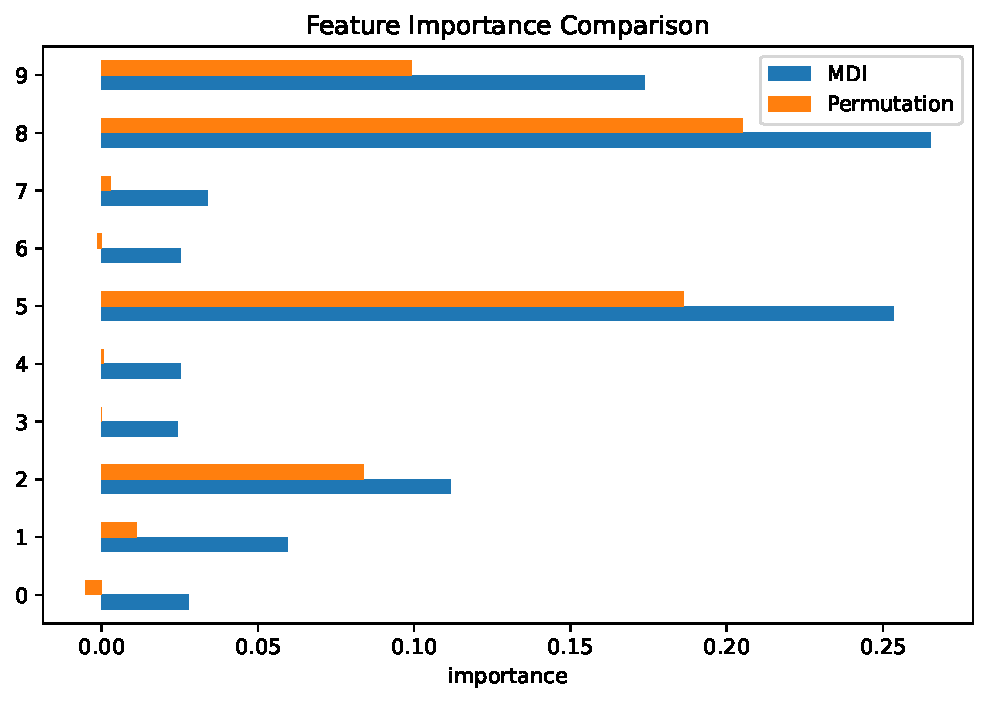
\includegraphics[keepaspectratio]{contents/2/rf_files/figure-pdf/cell-11-output-1.pdf}}

\section{Tuning Hyperparameters}\label{tuning-hyperparameters-1}

Bagging and random forests are usually easier to tune than boosting.
Still, several parameters matter.

{\def\LTcaptype{none} % do not increment counter
\begin{longtable}[]{@{}
  >{\raggedright\arraybackslash}p{(\linewidth - 2\tabcolsep) * \real{0.5000}}
  >{\raggedright\arraybackslash}p{(\linewidth - 2\tabcolsep) * \real{0.5000}}@{}}
\toprule\noalign{}
\begin{minipage}[b]{\linewidth}\raggedright
Parameter
\end{minipage} & \begin{minipage}[b]{\linewidth}\raggedright
Main effect
\end{minipage} \\
\midrule\noalign{}
\endhead
\bottomrule\noalign{}
\endlastfoot
\texttt{n\_estimators} & More trees reduce Monte Carlo variation, but
increase computation. \\
\texttt{max\_features} & Controls tree correlation. Smaller values
create more randomness. \\
\texttt{max\_samples} & Controls bootstrap sample size. Smaller values
create more diversity. \\
\texttt{min\_samples\_leaf} & Controls smoothness of each tree. Larger
values reduce overfitting. \\
\texttt{max\_depth} & Limits tree depth. Often left as \texttt{None},
but can help noisy data. \\
\end{longtable}
}

A practical tuning strategy is:

\begin{enumerate}
\def\labelenumi{\arabic{enumi}.}
\tightlist
\item
  Choose a reasonably large \texttt{n\_estimators} (so it is highly
  possible to be stable).
\item
  Tune \texttt{max\_features}, \texttt{min\_samples\_leaf},
  \texttt{max\_samples} or \texttt{max\_depth} with cross-validation or
  OOB error.
\item
  Make \texttt{n\_estimators} smaller to find the smallest stable
  number.
\end{enumerate}

\begin{tcolorbox}[enhanced jigsaw, arc=.35mm, bottomrule=.15mm, bottomtitle=1mm, breakable, colback=white, colbacktitle=quarto-callout-warning-color!10!white, colframe=quarto-callout-warning-color-frame, coltitle=black, left=2mm, leftrule=.75mm, opacityback=0, opacitybacktitle=0.6, rightrule=.15mm, title=\textcolor{quarto-callout-warning-color}{\faExclamationTriangle}\hspace{0.5em}{\texttt{n\_estimators}}, titlerule=0mm, toprule=.15mm, toptitle=1mm]

For bagging / random forests, \texttt{n\_estimators} is usually not a
regularization parameter in the usual sense. Increasing the number of
trees usually stabilizes the model rather than causing overfitting. The
main cost is computation. Therefore when reading the score vs number of
trees plot, we are not looking at the highest score, we are looking at
when the score is stablizing.

\end{tcolorbox}

\begin{tcolorbox}[enhanced jigsaw, arc=.35mm, bottomrule=.15mm, bottomtitle=1mm, breakable, colback=white, colbacktitle=quarto-callout-warning-color!10!white, colframe=quarto-callout-warning-color-frame, coltitle=black, left=2mm, leftrule=.75mm, opacityback=0, opacitybacktitle=0.6, rightrule=.15mm, title=\textcolor{quarto-callout-warning-color}{\faExclamationTriangle}\hspace{0.5em}{\texttt{1} and \texttt{1.0}}, titlerule=0mm, toprule=.15mm, toptitle=1mm]

These two represent different things.

\begin{itemize}
\tightlist
\item
  \texttt{max\_samples=1} means that the max number of samples we choose
  is 1.
\item
  \texttt{max\_samples=1.0} means that we want to choose all samples
  that the percent is 1.0=100\%.
\end{itemize}

\end{tcolorbox}

\begin{tcolorbox}[enhanced jigsaw, arc=.35mm, bottomrule=.15mm, bottomtitle=1mm, breakable, colback=white, colbacktitle=quarto-callout-note-color!10!white, colframe=quarto-callout-note-color-frame, coltitle=black, left=2mm, leftrule=.75mm, opacityback=0, opacitybacktitle=0.6, rightrule=.15mm, title=\textcolor{quarto-callout-note-color}{\faInfo}\hspace{0.5em}{Note}, titlerule=0mm, toprule=.15mm, toptitle=1mm]

Comparing to single tree/boosting, we tend to use larger trees in
bagging. Therefore we don't need \texttt{ccp\_alpha}, and we could use
larger \texttt{max\_depth} and smaller \texttt{min\_samples\_leaf}.

\end{tcolorbox}

\begin{tcolorbox}[enhanced jigsaw, arc=.35mm, bottomrule=.15mm, bottomtitle=1mm, breakable, colback=white, colbacktitle=quarto-callout-note-color!10!white, colframe=quarto-callout-note-color-frame, coltitle=black, left=2mm, leftrule=.75mm, opacityback=0, opacitybacktitle=0.6, rightrule=.15mm, title=\textcolor{quarto-callout-note-color}{\faInfo}\hspace{0.5em}{OOB validation}, titlerule=0mm, toprule=.15mm, toptitle=1mm]

We could use oob score to tune hyperparameters. However we have to
manually write the tuning code.

\begin{Shaded}
\begin{Highlighting}[]
\ImportTok{from}\NormalTok{ sklearn.ensemble }\ImportTok{import}\NormalTok{ RandomForestClassifier}

\NormalTok{max\_features\_list }\OperatorTok{=}\NormalTok{ [}\FloatTok{0.3}\NormalTok{, }\FloatTok{0.5}\NormalTok{, }\FloatTok{0.8}\NormalTok{, }\FloatTok{1.0}\NormalTok{]}
\NormalTok{best\_score }\OperatorTok{=} \OperatorTok{{-}}\DecValTok{1}
\NormalTok{best\_param }\OperatorTok{=} \VariableTok{None}

\ControlFlowTok{for}\NormalTok{ mf }\KeywordTok{in}\NormalTok{ max\_features\_list:}
\NormalTok{    rf }\OperatorTok{=}\NormalTok{ RandomForestClassifier(}
\NormalTok{        n\_estimators}\OperatorTok{=}\DecValTok{300}\NormalTok{, max\_features}\OperatorTok{=}\NormalTok{mf, oob\_score}\OperatorTok{=}\VariableTok{True}\NormalTok{, random\_state}\OperatorTok{=}\DecValTok{0}\NormalTok{, n\_jobs}\OperatorTok{={-}}\DecValTok{1}
\NormalTok{    )}
\NormalTok{    rf.fit(X\_train, y\_train)}
    \ControlFlowTok{if}\NormalTok{ rf.oob\_score\_ }\OperatorTok{\textgreater{}}\NormalTok{ best\_score:}
\NormalTok{        best\_score }\OperatorTok{=}\NormalTok{ rf.oob\_score\_}
\NormalTok{        best\_param }\OperatorTok{=}\NormalTok{ mf}

\BuiltInTok{print}\NormalTok{(best\_param)}
\end{Highlighting}
\end{Shaded}

\begin{verbatim}
0.3
\end{verbatim}

\end{tcolorbox}

\begin{tcolorbox}[enhanced jigsaw, arc=.35mm, bottomrule=.15mm, bottomtitle=1mm, breakable, colback=white, colbacktitle=quarto-callout-note-color!10!white, colframe=quarto-callout-note-color-frame, coltitle=black, left=2mm, leftrule=.75mm, opacityback=0, opacitybacktitle=0.6, rightrule=.15mm, title=\textcolor{quarto-callout-note-color}{\faInfo}\hspace{0.5em}{Cross-validation}, titlerule=0mm, toprule=.15mm, toptitle=1mm]

We could still use cross-validation to tune a random forest classifier.

\begin{Shaded}
\begin{Highlighting}[]
\ImportTok{from}\NormalTok{ sklearn.model\_selection }\ImportTok{import}\NormalTok{ GridSearchCV}
\ImportTok{from}\NormalTok{ sklearn.ensemble }\ImportTok{import}\NormalTok{ RandomForestClassifier}

\NormalTok{param\_grid }\OperatorTok{=}\NormalTok{ \{}
    \StringTok{"max\_features"}\NormalTok{: [}\FloatTok{0.3}\NormalTok{, }\FloatTok{0.6}\NormalTok{, }\FloatTok{1.0}\NormalTok{],}
    \StringTok{"min\_samples\_leaf"}\NormalTok{: [}\DecValTok{1}\NormalTok{, }\DecValTok{3}\NormalTok{, }\DecValTok{5}\NormalTok{],}
    \StringTok{"max\_samples"}\NormalTok{: [}\FloatTok{0.6}\NormalTok{, }\FloatTok{0.8}\NormalTok{, }\FloatTok{1.0}\NormalTok{],}
\NormalTok{\}}

\NormalTok{rf }\OperatorTok{=}\NormalTok{ RandomForestClassifier(n\_estimators}\OperatorTok{=}\DecValTok{300}\NormalTok{, random\_state}\OperatorTok{=}\DecValTok{0}\NormalTok{)}

\NormalTok{grid }\OperatorTok{=}\NormalTok{ GridSearchCV(rf, param\_grid}\OperatorTok{=}\NormalTok{param\_grid, cv}\OperatorTok{=}\DecValTok{5}\NormalTok{, n\_jobs}\OperatorTok{={-}}\DecValTok{1}\NormalTok{)}

\NormalTok{grid.fit(X\_train, y\_train)}

\NormalTok{best\_rf }\OperatorTok{=}\NormalTok{ grid.best\_estimator\_}
\NormalTok{grid.best\_params\_}
\end{Highlighting}
\end{Shaded}

\begin{verbatim}
{'max_features': 0.3, 'max_samples': 0.8, 'min_samples_leaf': 1}
\end{verbatim}

\end{tcolorbox}

\begin{tcolorbox}[enhanced jigsaw, arc=.35mm, bottomrule=.15mm, bottomtitle=1mm, breakable, colback=white, colbacktitle=quarto-callout-note-color!10!white, colframe=quarto-callout-note-color-frame, coltitle=black, left=2mm, leftrule=.75mm, opacityback=0, opacitybacktitle=0.6, rightrule=.15mm, title=\textcolor{quarto-callout-note-color}{\faInfo}\hspace{0.5em}{Randomized Search}, titlerule=0mm, toprule=.15mm, toptitle=1mm]

If the dataset is large, a full grid can be slow. In that case,
\texttt{RandomizedSearchCV} is often a better choice. In this case, only
a few random combinations will be searched. In the following example, we
only search 30 combinations.

\begin{Shaded}
\begin{Highlighting}[]
\ImportTok{from}\NormalTok{ sklearn.model\_selection }\ImportTok{import}\NormalTok{ RandomizedSearchCV}
\ImportTok{from}\NormalTok{ scipy.stats }\ImportTok{import}\NormalTok{ randint, uniform}

\NormalTok{param\_dist }\OperatorTok{=}\NormalTok{ \{}
    \StringTok{"max\_features"}\NormalTok{: uniform(}\FloatTok{0.2}\NormalTok{, }\FloatTok{0.8}\NormalTok{),}
    \StringTok{"min\_samples\_leaf"}\NormalTok{: randint(}\DecValTok{1}\NormalTok{, }\DecValTok{20}\NormalTok{),}
    \StringTok{"max\_samples"}\NormalTok{: uniform(}\FloatTok{0.5}\NormalTok{, }\FloatTok{0.5}\NormalTok{),}
\NormalTok{\}}

\NormalTok{rf }\OperatorTok{=}\NormalTok{ RandomForestClassifier(n\_estimators}\OperatorTok{=}\DecValTok{300}\NormalTok{, random\_state}\OperatorTok{=}\DecValTok{0}\NormalTok{)}

\NormalTok{search }\OperatorTok{=}\NormalTok{ RandomizedSearchCV(}
\NormalTok{    rf, param\_distributions}\OperatorTok{=}\NormalTok{param\_dist, n\_iter}\OperatorTok{=}\DecValTok{30}\NormalTok{, cv}\OperatorTok{=}\DecValTok{5}\NormalTok{, random\_state}\OperatorTok{=}\DecValTok{0}\NormalTok{, n\_jobs}\OperatorTok{={-}}\DecValTok{1}
\NormalTok{)}

\NormalTok{search.fit(X\_train, y\_train)}
\NormalTok{search.best\_params\_}
\end{Highlighting}
\end{Shaded}

\begin{verbatim}
{'max_features': np.float64(0.9220787804235238),
 'max_samples': np.float64(0.7249749949556138),
 'min_samples_leaf': 2}
\end{verbatim}

\end{tcolorbox}

\subsection{\texorpdfstring{\texttt{n\_jobs}}{n\_jobs}}\label{n_jobs-1}

When we reach this stage, you may notice that training can become quite
slow. This is expected because, in \texttt{GridSearchCV}, we need to
evaluate many combinations of hyperparameters. For each combination, we
may need to train many trees (due to bagging or Random Forests), and the
entire process must be repeated multiple times because of
cross-validation (for example, \texttt{cv=5}).

Although many models need to be trained, an important advantage is that
these training tasks are largely independent. Therefore, they can often
be trained simultaneously using multiple CPU cores.

In contrast, boosting methods that we will discuss later are
fundamentally sequential. Each tree depends on the results of the
previous trees, so the trees must be trained one after another. As a
result, boosting methods are generally less parallelizable at the tree
level.

\texttt{sklearn} supports multi-core CPUs through the \texttt{n\_jobs}
argument.

\begin{itemize}
\tightlist
\item
  \texttt{n\_jobs=1} means single-core execution
\item
  \texttt{n\_jobs=k} uses exactly \texttt{k} CPU cores
\item
  \texttt{n\_jobs=-1} uses all available CPU cores
\item
  \texttt{n\_jobs=None} uses the library default, which is currently
  equivalent to \texttt{1} in most \texttt{sklearn} functions
\end{itemize}

Many functions in \texttt{sklearn} support this argument. For details,
consult the official documentation for the specific function being used.

One important practical issue is nested parallelism. When multiple
nested functions both support \texttt{n\_jobs}, it is usually best to
parallelize only the outermost function.

For example,
\texttt{GridSearchCV(RandomForestClassifier(n\_jobs=1),\ n\_jobs=-1)} is
generally preferred over
\texttt{GridSearchCV(RandomForestClassifier(n\_jobs=-1),\ n\_jobs=-1)}
because allowing both levels to parallelize simultaneously may create
too many worker processes or threads, leading to excessive overhead and
sometimes even slower performance.

\begin{example}[time it]\protect\hypertarget{exm-}{}\label{exm-}

We first write a helper function to compute the runtime.

\begin{Shaded}
\begin{Highlighting}[]
\ImportTok{from}\NormalTok{ time }\ImportTok{import}\NormalTok{ perf\_counter}
\ImportTok{from}\NormalTok{ contextlib }\ImportTok{import}\NormalTok{ contextmanager}

\AttributeTok{@contextmanager}
\KeywordTok{def}\NormalTok{ timer(name}\OperatorTok{=}\StringTok{"runtime"}\NormalTok{):}
\NormalTok{    start }\OperatorTok{=}\NormalTok{ perf\_counter()}
    \ControlFlowTok{yield}
\NormalTok{    end }\OperatorTok{=}\NormalTok{ perf\_counter()}

    \BuiltInTok{print}\NormalTok{(}\SpecialStringTok{f"}\SpecialCharTok{\{}\NormalTok{name}\SpecialCharTok{\}}\SpecialStringTok{: }\SpecialCharTok{\{}\NormalTok{end }\OperatorTok{{-}}\NormalTok{ start}\SpecialCharTok{:.4f\}}\SpecialStringTok{ seconds"}\NormalTok{)}
\end{Highlighting}
\end{Shaded}

Then use it to test the time for different \texttt{n\_jobs}.

\begin{Shaded}
\begin{Highlighting}[]
\NormalTok{param\_grid }\OperatorTok{=}\NormalTok{ \{}
    \StringTok{"max\_features"}\NormalTok{: [}\FloatTok{0.3}\NormalTok{, }\FloatTok{0.6}\NormalTok{, }\FloatTok{1.0}\NormalTok{],}
    \StringTok{"min\_samples\_leaf"}\NormalTok{: [}\DecValTok{1}\NormalTok{, }\DecValTok{3}\NormalTok{, }\DecValTok{5}\NormalTok{],}
    \StringTok{"max\_samples"}\NormalTok{: [}\FloatTok{0.6}\NormalTok{, }\FloatTok{0.8}\NormalTok{, }\FloatTok{1.0}\NormalTok{],}
\NormalTok{\}}

\NormalTok{rf }\OperatorTok{=}\NormalTok{ RandomForestClassifier(n\_estimators}\OperatorTok{=}\DecValTok{300}\NormalTok{, random\_state}\OperatorTok{=}\DecValTok{0}\NormalTok{)}

\NormalTok{grid }\OperatorTok{=}\NormalTok{ GridSearchCV(rf, param\_grid}\OperatorTok{=}\NormalTok{param\_grid, cv}\OperatorTok{=}\DecValTok{5}\NormalTok{, n\_jobs}\OperatorTok{={-}}\DecValTok{1}\NormalTok{)}
\ControlFlowTok{with}\NormalTok{ timer(}\StringTok{"n\_jobs={-}1"}\NormalTok{):}
\NormalTok{    grid.fit(X\_train, y\_train)}

\NormalTok{grid }\OperatorTok{=}\NormalTok{ GridSearchCV(rf, param\_grid}\OperatorTok{=}\NormalTok{param\_grid, cv}\OperatorTok{=}\DecValTok{5}\NormalTok{, n\_jobs}\OperatorTok{=}\DecValTok{1}\NormalTok{)}
\ControlFlowTok{with}\NormalTok{ timer(}\StringTok{"n\_jobs=1"}\NormalTok{):}
\NormalTok{    grid.fit(X\_train, y\_train)}
\end{Highlighting}
\end{Shaded}

\begin{verbatim}
n_jobs=-1: 27.2958 seconds
n_jobs=1: 84.3413 seconds
\end{verbatim}

\end{example}

\section{Example: Diabetes dataset}\label{example-diabetes-dataset}

We now use the diabetes regression dataset from \texttt{sklearn}. In
order to compare results using trees, we use the same split with
\texttt{random\_state=1}.

\begin{Shaded}
\begin{Highlighting}[]
\ImportTok{import}\NormalTok{ numpy }\ImportTok{as}\NormalTok{ np}
\ImportTok{import}\NormalTok{ pandas }\ImportTok{as}\NormalTok{ pd}
\ImportTok{import}\NormalTok{ matplotlib.pyplot }\ImportTok{as}\NormalTok{ plt}

\ImportTok{from}\NormalTok{ sklearn.datasets }\ImportTok{import}\NormalTok{ load\_diabetes}
\ImportTok{from}\NormalTok{ sklearn.model\_selection }\ImportTok{import}\NormalTok{ train\_test\_split}
\ImportTok{from}\NormalTok{ sklearn.metrics }\ImportTok{import}\NormalTok{ mean\_squared\_error, r2\_score}

\NormalTok{X, y }\OperatorTok{=}\NormalTok{ load\_diabetes(return\_X\_y}\OperatorTok{=}\VariableTok{True}\NormalTok{)}

\NormalTok{X\_train, X\_test, y\_train, y\_test }\OperatorTok{=}\NormalTok{ train\_test\_split(X, y, test\_size}\OperatorTok{=}\FloatTok{0.2}\NormalTok{, random\_state}\OperatorTok{=}\DecValTok{1}\NormalTok{)}
\end{Highlighting}
\end{Shaded}

We compare three models:

\begin{enumerate}
\def\labelenumi{\arabic{enumi}.}
\tightlist
\item
  a single regression tree,
\item
  bagging with regression trees,
\item
  a random forest.
\end{enumerate}

\begin{Shaded}
\begin{Highlighting}[]
\ImportTok{from}\NormalTok{ sklearn.tree }\ImportTok{import}\NormalTok{ DecisionTreeRegressor}
\ImportTok{from}\NormalTok{ sklearn.ensemble }\ImportTok{import}\NormalTok{ BaggingRegressor, RandomForestRegressor}

\NormalTok{tree }\OperatorTok{=}\NormalTok{ DecisionTreeRegressor(random\_state}\OperatorTok{=}\DecValTok{1}\NormalTok{, ccp\_alpha}\OperatorTok{=}\FloatTok{105.185}\NormalTok{)}

\NormalTok{bag }\OperatorTok{=}\NormalTok{ BaggingRegressor(}
\NormalTok{    estimator}\OperatorTok{=}\NormalTok{DecisionTreeRegressor(random\_state}\OperatorTok{=}\DecValTok{1}\NormalTok{),}
\NormalTok{    n\_estimators}\OperatorTok{=}\DecValTok{300}\NormalTok{,}
\NormalTok{    oob\_score}\OperatorTok{=}\VariableTok{True}\NormalTok{,}
\NormalTok{    random\_state}\OperatorTok{=}\DecValTok{1}\NormalTok{,}
\NormalTok{)}

\NormalTok{rf }\OperatorTok{=}\NormalTok{ RandomForestRegressor(}
\NormalTok{    n\_estimators}\OperatorTok{=}\DecValTok{300}\NormalTok{,}
\NormalTok{    max\_features}\OperatorTok{=}\StringTok{"sqrt"}\NormalTok{,}
\NormalTok{    oob\_score}\OperatorTok{=}\VariableTok{True}\NormalTok{,}
\NormalTok{    random\_state}\OperatorTok{=}\DecValTok{1}\NormalTok{,}
\NormalTok{)}
\end{Highlighting}
\end{Shaded}

\begin{Shaded}
\begin{Highlighting}[]
\NormalTok{tree.fit(X\_train, y\_train)}
\NormalTok{tree.score(X\_test, y\_test)}
\end{Highlighting}
\end{Shaded}

\begin{verbatim}
0.1922738375305083
\end{verbatim}

\begin{Shaded}
\begin{Highlighting}[]
\NormalTok{bag.fit(X\_train, y\_train)}
\NormalTok{bag.score(X\_test, y\_test)}
\end{Highlighting}
\end{Shaded}

\begin{verbatim}
0.2951908085625511
\end{verbatim}

\begin{Shaded}
\begin{Highlighting}[]
\NormalTok{rf.fit(X\_train, y\_train)}
\NormalTok{rf.score(X\_test, y\_test)}
\end{Highlighting}
\end{Shaded}

\begin{verbatim}
0.3555401846697034
\end{verbatim}

The single tree is expected to be unstable. Bagging and random forests
usually improve test performance by averaging many trees.

For the bagging and random forest models, we can also check OOB
performance.

\begin{Shaded}
\begin{Highlighting}[]
\NormalTok{bag.oob\_score\_}
\end{Highlighting}
\end{Shaded}

\begin{verbatim}
0.4567923788468702
\end{verbatim}

\begin{Shaded}
\begin{Highlighting}[]
\NormalTok{rf.oob\_score\_}
\end{Highlighting}
\end{Shaded}

\begin{verbatim}
0.47245609860472904
\end{verbatim}

OOB \(R^2\) gives an internal estimate of predictive performance based
only on the training data.

\subsection{Tuning the Random Forest}\label{tuning-the-random-forest}

We showed \texttt{Bagging} in the previous section. Since it overlaps
with \texttt{RandomForest}, we will only focus on the Random Forest
model in this section. We first tune \texttt{max\_features},
\texttt{min\_samples\_leaf}, and \texttt{max\_samples} by
cross-validation, with a relative small number of estimators.

\begin{Shaded}
\begin{Highlighting}[]
\ImportTok{from}\NormalTok{ sklearn.model\_selection }\ImportTok{import}\NormalTok{ GridSearchCV}

\NormalTok{rf\_base }\OperatorTok{=}\NormalTok{ RandomForestRegressor(n\_estimators}\OperatorTok{=}\DecValTok{300}\NormalTok{, random\_state}\OperatorTok{=}\DecValTok{1}\NormalTok{)}

\NormalTok{param\_grid }\OperatorTok{=}\NormalTok{ \{}
    \StringTok{"max\_features"}\NormalTok{: [}\StringTok{"sqrt"}\NormalTok{, }\FloatTok{0.5}\NormalTok{, }\FloatTok{1.0}\NormalTok{],}
    \StringTok{"min\_samples\_leaf"}\NormalTok{: [}\DecValTok{1}\NormalTok{, }\DecValTok{3}\NormalTok{, }\DecValTok{5}\NormalTok{, }\DecValTok{10}\NormalTok{],}
    \StringTok{"max\_samples"}\NormalTok{: [}\FloatTok{0.6}\NormalTok{, }\FloatTok{0.8}\NormalTok{, }\FloatTok{1.0}\NormalTok{],}
\NormalTok{\}}

\NormalTok{grid }\OperatorTok{=}\NormalTok{ GridSearchCV(rf\_base, param\_grid}\OperatorTok{=}\NormalTok{param\_grid, cv}\OperatorTok{=}\DecValTok{5}\NormalTok{, n\_jobs}\OperatorTok{={-}}\DecValTok{1}\NormalTok{)}

\NormalTok{grid.fit(X\_train, y\_train)}

\BuiltInTok{print}\NormalTok{(}\SpecialStringTok{f"Best parameters: }\SpecialCharTok{\{}\NormalTok{grid}\SpecialCharTok{.}\NormalTok{best\_params\_}\SpecialCharTok{\}}\SpecialStringTok{"}\NormalTok{)}
\BuiltInTok{print}\NormalTok{(}\SpecialStringTok{f"Best CV R\^{}2: }\SpecialCharTok{\{}\NormalTok{grid}\SpecialCharTok{.}\NormalTok{best\_score\_}\SpecialCharTok{\}}\SpecialStringTok{"}\NormalTok{)}
\end{Highlighting}
\end{Shaded}

\begin{verbatim}
Best parameters: {'max_features': 'sqrt', 'max_samples': 1.0, 'min_samples_leaf': 5}
Best CV R^2: 0.45220837115313606
\end{verbatim}

Now evaluate the tuned model on the test set.

\begin{Shaded}
\begin{Highlighting}[]
\NormalTok{grid.best\_estimator\_.score(X\_test, y\_test)}
\end{Highlighting}
\end{Shaded}

\begin{verbatim}
0.3777186499485139
\end{verbatim}

\subsection{Find the Number of Trees}\label{find-the-number-of-trees}

The number of trees controls how stable the ensemble average is. The
following code fits forests with different numbers of trees and records
OOB performance.

\begin{Shaded}
\begin{Highlighting}[]
\NormalTok{tree\_counts }\OperatorTok{=}\NormalTok{ [}\DecValTok{10}\NormalTok{, }\DecValTok{25}\NormalTok{, }\DecValTok{50}\NormalTok{, }\DecValTok{100}\NormalTok{, }\DecValTok{200}\NormalTok{, }\DecValTok{300}\NormalTok{, }\DecValTok{400}\NormalTok{, }\DecValTok{800}\NormalTok{]}
\NormalTok{oob\_scores }\OperatorTok{=}\NormalTok{ []}
\NormalTok{test\_r2 }\OperatorTok{=}\NormalTok{ []}

\ControlFlowTok{for}\NormalTok{ n\_trees }\KeywordTok{in}\NormalTok{ tree\_counts:}
\NormalTok{    model }\OperatorTok{=}\NormalTok{ RandomForestRegressor(}
\NormalTok{        n\_estimators}\OperatorTok{=}\NormalTok{n\_trees,}
\NormalTok{        max\_features}\OperatorTok{=}\StringTok{"sqrt"}\NormalTok{,}
\NormalTok{        max\_samples}\OperatorTok{=}\FloatTok{1.0}\NormalTok{,}
\NormalTok{        min\_samples\_leaf}\OperatorTok{=}\DecValTok{5}\NormalTok{,}
\NormalTok{        oob\_score}\OperatorTok{=}\VariableTok{True}\NormalTok{,}
\NormalTok{        random\_state}\OperatorTok{=}\DecValTok{1}\NormalTok{,}
\NormalTok{        n\_jobs}\OperatorTok{={-}}\DecValTok{1}\NormalTok{,}
\NormalTok{    )}
\NormalTok{    model.fit(X\_train, y\_train)}
\NormalTok{    oob\_scores.append(model.oob\_score\_)}
\NormalTok{    test\_r2.append(model.score(X\_test, y\_test))}

\NormalTok{fig, ax }\OperatorTok{=}\NormalTok{ plt.subplots(}\DecValTok{1}\NormalTok{, }\DecValTok{2}\NormalTok{, figsize}\OperatorTok{=}\NormalTok{(}\DecValTok{11}\NormalTok{, }\DecValTok{4}\NormalTok{))}

\NormalTok{ax[}\DecValTok{0}\NormalTok{].plot(tree\_counts, oob\_scores, marker}\OperatorTok{=}\StringTok{"o"}\NormalTok{)}
\NormalTok{ax[}\DecValTok{0}\NormalTok{].set\_xlabel(}\StringTok{"number of trees"}\NormalTok{)}
\NormalTok{ax[}\DecValTok{0}\NormalTok{].set\_ylabel(}\StringTok{"OOB R\^{}2"}\NormalTok{)}
\NormalTok{ax[}\DecValTok{0}\NormalTok{].set\_title(}\StringTok{"OOB score"}\NormalTok{)}

\NormalTok{ax[}\DecValTok{1}\NormalTok{].plot(tree\_counts, test\_r2, marker}\OperatorTok{=}\StringTok{"o"}\NormalTok{)}
\NormalTok{ax[}\DecValTok{1}\NormalTok{].set\_xlabel(}\StringTok{"number of trees"}\NormalTok{)}
\NormalTok{ax[}\DecValTok{1}\NormalTok{].set\_ylabel(}\StringTok{"test R\^{}2"}\NormalTok{)}
\NormalTok{ax[}\DecValTok{1}\NormalTok{].set\_title(}\StringTok{"Validation score (using test set)"}\NormalTok{)}\OperatorTok{;}
\end{Highlighting}
\end{Shaded}

\pandocbounded{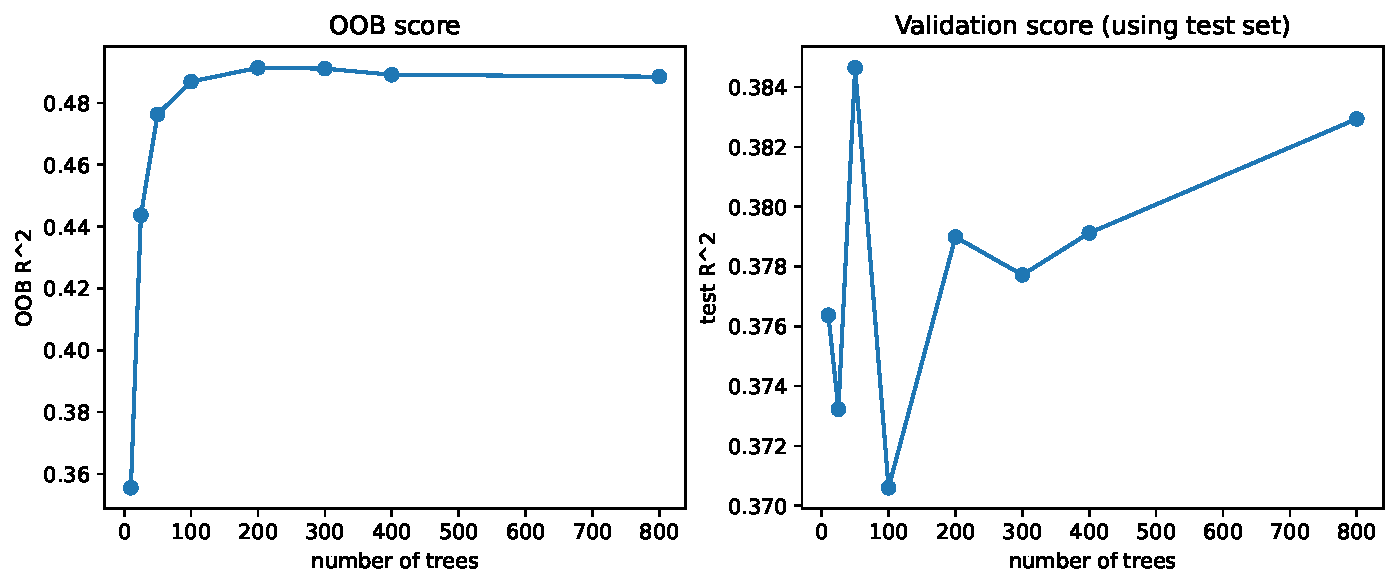
\includegraphics[keepaspectratio]{contents/2/rf_files/figure-pdf/cell-26-output-1.pdf}}

As mentioned previously, when reading these two plots, it is important
not to focus on the single highest point. Instead, we look for the point
where the curve becomes stable and nearly flat. In this example, around
200 trees appears to be a reasonable choice.

Therefore our best model so far is

\begin{Shaded}
\begin{Highlighting}[]
\NormalTok{best\_rf }\OperatorTok{=}\NormalTok{ RandomForestRegressor(}
\NormalTok{    n\_estimators}\OperatorTok{=}\DecValTok{200}\NormalTok{,}
\NormalTok{    max\_features}\OperatorTok{=}\StringTok{"sqrt"}\NormalTok{,}
\NormalTok{    max\_samples}\OperatorTok{=}\FloatTok{1.0}\NormalTok{,}
\NormalTok{    min\_samples\_leaf}\OperatorTok{=}\DecValTok{5}\NormalTok{,}
\NormalTok{    oob\_score}\OperatorTok{=}\VariableTok{True}\NormalTok{,}
\NormalTok{    random\_state}\OperatorTok{=}\DecValTok{1}\NormalTok{,}
\NormalTok{    n\_jobs}\OperatorTok{={-}}\DecValTok{1}
\NormalTok{)}
\NormalTok{best\_rf.fit(X\_train, y\_train)}
\end{Highlighting}
\end{Shaded}

{\def\LTcaptype{none} % do not increment counter
\begin{longtable}[]{@{}
  >{\raggedright\arraybackslash}p{(\linewidth - 4\tabcolsep) * \real{0.3333}}
  >{\raggedright\arraybackslash}p{(\linewidth - 4\tabcolsep) * \real{0.3333}}
  >{\raggedright\arraybackslash}p{(\linewidth - 4\tabcolsep) * \real{0.3333}}@{}}
\toprule\noalign{}
\endhead
\bottomrule\noalign{}
\endlastfoot
\emph{} & \begin{minipage}[t]{\linewidth}\raggedright
\href{https://scikit-learn.org/1.8/modules/generated/sklearn.ensemble.RandomForestRegressor.html\#:~:text=n_estimators,-int\%2C\%20default\%3D100}{n\_estimators
{n\_estimators: int, default=100\\
\strut \\
The number of trees in the forest.\\
\strut \\
.. versionchanged:: 0.22\\
The default value of ``n\_estimators`` changed from 10 to 100\\
in 0.22.}}\strut
\end{minipage} & 200 \\
\emph{} & \begin{minipage}[t]{\linewidth}\raggedright
\href{https://scikit-learn.org/1.8/modules/generated/sklearn.ensemble.RandomForestRegressor.html\#:~:text=criterion,-\%7B\%22squared_error\%22\%2C\%20\%22absolute_error\%22\%2C\%20\%22friedman_mse\%22\%2C\%20\%22poisson\%22\%7D\%2C\%20\%20\%20\%20\%20\%20\%20\%20\%20\%20\%20\%20\%20default\%3D\%22squared_error\%22}{criterion
{criterion: \{"squared\_error", "absolute\_error", "friedman\_mse",
"poisson"\}, default="squared\_error"\\
\strut \\
The function to measure the quality of a split. Supported criteria\\
are "squared\_error" for the mean squared error, which is equal to\\
variance reduction as feature selection criterion and minimizes the L2\\
loss using the mean of each terminal node, "friedman\_mse", which uses\\
mean squared error with Friedman\textquotesingle s improvement score for
potential\\
splits, "absolute\_error" for the mean absolute error, which minimizes\\
the L1 loss using the median of each terminal node, and "poisson"
which\\
uses reduction in Poisson deviance to find splits.\\
Training using "absolute\_error" is significantly slower\\
than when using "squared\_error".\\
\strut \\
.. versionadded:: 0.18\\
Mean Absolute Error (MAE) criterion.\\
\strut \\
.. versionadded:: 1.0\\
Poisson criterion.}}\strut
\end{minipage} & \textquotesingle squared\_error\textquotesingle{} \\
\emph{} & \begin{minipage}[t]{\linewidth}\raggedright
\href{https://scikit-learn.org/1.8/modules/generated/sklearn.ensemble.RandomForestRegressor.html\#:~:text=max_depth,-int\%2C\%20default\%3DNone}{max\_depth
{max\_depth: int, default=None\\
\strut \\
The maximum depth of the tree. If None, then nodes are expanded until\\
all leaves are pure or until all leaves contain less than\\
min\_samples\_split samples.}}\strut
\end{minipage} & None \\
\emph{} & \begin{minipage}[t]{\linewidth}\raggedright
\href{https://scikit-learn.org/1.8/modules/generated/sklearn.ensemble.RandomForestRegressor.html\#:~:text=min_samples_split,-int\%20or\%20float\%2C\%20default\%3D2}{min\_samples\_split
{min\_samples\_split: int or float, default=2\\
\strut \\
The minimum number of samples required to split an internal node:\\
\strut \\
- If int, then consider `min\_samples\_split` as the minimum number.\\
- If float, then `min\_samples\_split` is a fraction and\\
`ceil(min\_samples\_split * n\_samples)` are the minimum\\
number of samples for each split.\\
\strut \\
.. versionchanged:: 0.18\\
Added float values for fractions.}}\strut
\end{minipage} & 2 \\
\emph{} & \begin{minipage}[t]{\linewidth}\raggedright
\href{https://scikit-learn.org/1.8/modules/generated/sklearn.ensemble.RandomForestRegressor.html\#:~:text=min_samples_leaf,-int\%20or\%20float\%2C\%20default\%3D1}{min\_samples\_leaf
{min\_samples\_leaf: int or float, default=1\\
\strut \\
The minimum number of samples required to be at a leaf node.\\
A split point at any depth will only be considered if it leaves at\\
least ``min\_samples\_leaf`` training samples in each of the left and\\
right branches. This may have the effect of smoothing the model,\\
especially in regression.\\
\strut \\
- If int, then consider `min\_samples\_leaf` as the minimum number.\\
- If float, then `min\_samples\_leaf` is a fraction and\\
`ceil(min\_samples\_leaf * n\_samples)` are the minimum\\
number of samples for each node.\\
\strut \\
.. versionchanged:: 0.18\\
Added float values for fractions.}}\strut
\end{minipage} & 5 \\
\emph{} & \begin{minipage}[t]{\linewidth}\raggedright
\href{https://scikit-learn.org/1.8/modules/generated/sklearn.ensemble.RandomForestRegressor.html\#:~:text=min_weight_fraction_leaf,-float\%2C\%20default\%3D0.0}{min\_weight\_fraction\_leaf
{min\_weight\_fraction\_leaf: float, default=0.0\\
\strut \\
The minimum weighted fraction of the sum total of weights (of all\\
the input samples) required to be at a leaf node. Samples have\\
equal weight when sample\_weight is not provided.}}\strut
\end{minipage} & 0.0 \\
\emph{} & \begin{minipage}[t]{\linewidth}\raggedright
\href{https://scikit-learn.org/1.8/modules/generated/sklearn.ensemble.RandomForestRegressor.html\#:~:text=max_features,-\%7B\%22sqrt\%22\%2C\%20\%22log2\%22\%2C\%20None\%7D\%2C\%20int\%20or\%20float\%2C\%20default\%3D1.0}{max\_features
{max\_features: \{"sqrt", "log2", None\}, int or float, default=1.0\\
\strut \\
The number of features to consider when looking for the best split:\\
\strut \\
- If int, then consider `max\_features` features at each split.\\
- If float, then `max\_features` is a fraction and\\
`max(1, int(max\_features * n\_features\_in\_))` features are considered
at each\\
split.\\
- If "sqrt", then `max\_features=sqrt(n\_features)`.\\
- If "log2", then `max\_features=log2(n\_features)`.\\
- If None or 1.0, then `max\_features=n\_features`.\\
\strut \\
.. note::\\
The default of 1.0 is equivalent to bagged trees and more\\
randomness can be achieved by setting smaller values, e.g. 0.3.\\
\strut \\
.. versionchanged:: 1.1\\
The default of `max\_features` changed from `"auto"` to 1.0.\\
\strut \\
Note: the search for a split does not stop until at least one\\
valid partition of the node samples is found, even if it requires to\\
effectively inspect more than ``max\_features`` features.}}\strut
\end{minipage} & \textquotesingle sqrt\textquotesingle{} \\
\emph{} & \begin{minipage}[t]{\linewidth}\raggedright
\href{https://scikit-learn.org/1.8/modules/generated/sklearn.ensemble.RandomForestRegressor.html\#:~:text=max_leaf_nodes,-int\%2C\%20default\%3DNone}{max\_leaf\_nodes
{max\_leaf\_nodes: int, default=None\\
\strut \\
Grow trees with ``max\_leaf\_nodes`` in best-first fashion.\\
Best nodes are defined as relative reduction in impurity.\\
If None then unlimited number of leaf nodes.}}\strut
\end{minipage} & None \\
\emph{} & \begin{minipage}[t]{\linewidth}\raggedright
\href{https://scikit-learn.org/1.8/modules/generated/sklearn.ensemble.RandomForestRegressor.html\#:~:text=min_impurity_decrease,-float\%2C\%20default\%3D0.0}{min\_impurity\_decrease
{min\_impurity\_decrease: float, default=0.0\\
\strut \\
A node will be split if this split induces a decrease of the impurity\\
greater than or equal to this value.\\
\strut \\
The weighted impurity decrease equation is the following::\\
\strut \\
N\_t / N * (impurity - N\_t\_R / N\_t * right\_impurity\\
- N\_t\_L / N\_t * left\_impurity)\\
\strut \\
where ``N`` is the total number of samples, ``N\_t`` is the number of\\
samples at the current node, ``N\_t\_L`` is the number of samples in
the\\
left child, and ``N\_t\_R`` is the number of samples in the right
child.\\
\strut \\
``N``, ``N\_t``, ``N\_t\_R`` and ``N\_t\_L`` all refer to the weighted
sum,\\
if ``sample\_weight`` is passed.\\
\strut \\
.. versionadded:: 0.19}}\strut
\end{minipage} & 0.0 \\
\emph{} & \begin{minipage}[t]{\linewidth}\raggedright
\href{https://scikit-learn.org/1.8/modules/generated/sklearn.ensemble.RandomForestRegressor.html\#:~:text=bootstrap,-bool\%2C\%20default\%3DTrue}{bootstrap
{bootstrap: bool, default=True\\
\strut \\
Whether bootstrap samples are used when building trees. If False, the\\
whole dataset is used to build each tree.}}\strut
\end{minipage} & True \\
\emph{} & \begin{minipage}[t]{\linewidth}\raggedright
\href{https://scikit-learn.org/1.8/modules/generated/sklearn.ensemble.RandomForestRegressor.html\#:~:text=oob_score,-bool\%20or\%20callable\%2C\%20default\%3DFalse}{oob\_score
{oob\_score: bool or callable, default=False\\
\strut \\
Whether to use out-of-bag samples to estimate the generalization
score.\\
By default, :func:`\textasciitilde sklearn.metrics.r2\_score` is used.\\
Provide a callable with signature `metric(y\_true, y\_pred)` to use a\\
custom metric. Only available if `bootstrap=True`.\\
\strut \\
For an illustration of out-of-bag (OOB) error estimation, see the
example\\
:ref:`sphx\_glr\_auto\_examples\_ensemble\_plot\_ensemble\_oob.py`.}}\strut
\end{minipage} & True \\
\emph{} & \begin{minipage}[t]{\linewidth}\raggedright
\href{https://scikit-learn.org/1.8/modules/generated/sklearn.ensemble.RandomForestRegressor.html\#:~:text=n_jobs,-int\%2C\%20default\%3DNone}{n\_jobs
{n\_jobs: int, default=None\\
\strut \\
The number of jobs to run in parallel. :meth:`fit`, :meth:`predict`,\\
:meth:`decision\_path` and :meth:`apply` are all parallelized over the\\
trees. ``None`` means 1 unless in a :obj:`joblib.parallel\_backend`\\
context. ``-1`` means using all processors. See :term:`Glossary\\
` for more details.}}\strut
\end{minipage} & -1 \\
\emph{} & \begin{minipage}[t]{\linewidth}\raggedright
\href{https://scikit-learn.org/1.8/modules/generated/sklearn.ensemble.RandomForestRegressor.html\#:~:text=random_state,-int\%2C\%20RandomState\%20instance\%20or\%20None\%2C\%20default\%3DNone}{random\_state
{random\_state: int, RandomState instance or None, default=None\\
\strut \\
Controls both the randomness of the bootstrapping of the samples used\\
when building trees (if ``bootstrap=True``) and the sampling of the\\
features to consider when looking for the best split at each node\\
(if ``max\_features \textless{} n\_features``).\\
See :term:`Glossary ` for details.}}\strut
\end{minipage} & 1 \\
\emph{} & \begin{minipage}[t]{\linewidth}\raggedright
\href{https://scikit-learn.org/1.8/modules/generated/sklearn.ensemble.RandomForestRegressor.html\#:~:text=verbose,-int\%2C\%20default\%3D0}{verbose
{verbose: int, default=0\\
\strut \\
Controls the verbosity when fitting and predicting.}}\strut
\end{minipage} & 0 \\
\emph{} & \begin{minipage}[t]{\linewidth}\raggedright
\href{https://scikit-learn.org/1.8/modules/generated/sklearn.ensemble.RandomForestRegressor.html\#:~:text=warm_start,-bool\%2C\%20default\%3DFalse}{warm\_start
{warm\_start: bool, default=False\\
\strut \\
When set to ``True``, reuse the solution of the previous call to fit\\
and add more estimators to the ensemble, otherwise, just fit a whole\\
new forest. See :term:`Glossary ` and\\
:ref:`tree\_ensemble\_warm\_start` for details.}}\strut
\end{minipage} & False \\
\emph{} & \begin{minipage}[t]{\linewidth}\raggedright
\href{https://scikit-learn.org/1.8/modules/generated/sklearn.ensemble.RandomForestRegressor.html\#:~:text=ccp_alpha,-non-negative\%20float\%2C\%20default\%3D0.0}{ccp\_alpha
{ccp\_alpha: non-negative float, default=0.0\\
\strut \\
Complexity parameter used for Minimal Cost-Complexity Pruning. The\\
subtree with the largest cost complexity that is smaller than\\
``ccp\_alpha`` will be chosen. By default, no pruning is performed.
See\\
:ref:`minimal\_cost\_complexity\_pruning` for details. See\\
:ref:`sphx\_glr\_auto\_examples\_tree\_plot\_cost\_complexity\_pruning.py`\\
for an example of such pruning.\\
\strut \\
.. versionadded:: 0.22}}\strut
\end{minipage} & 0.0 \\
\emph{} & \begin{minipage}[t]{\linewidth}\raggedright
\href{https://scikit-learn.org/1.8/modules/generated/sklearn.ensemble.RandomForestRegressor.html\#:~:text=max_samples,-int\%20or\%20float\%2C\%20default\%3DNone}{max\_samples
{max\_samples: int or float, default=None\\
\strut \\
If bootstrap is True, the number of samples to draw from X\\
to train each base estimator.\\
\strut \\
- If None (default), then draw `X.shape{[}0{]}` samples.\\
- If int, then draw `max\_samples` samples.\\
- If float, then draw `max(round(n\_samples * max\_samples), 1)`
samples. Thus,\\
`max\_samples` should be in the interval `(0.0, 1.0{]}`.\\
\strut \\
.. versionadded:: 0.22}}\strut
\end{minipage} & 1.0 \\
\emph{} & \begin{minipage}[t]{\linewidth}\raggedright
\href{https://scikit-learn.org/1.8/modules/generated/sklearn.ensemble.RandomForestRegressor.html\#:~:text=monotonic_cst,-array-like\%20of\%20int\%20of\%20shape\%20\%28n_features\%29\%2C\%20default\%3DNone}{monotonic\_cst
{monotonic\_cst: array-like of int of shape (n\_features),
default=None\\
\strut \\
Indicates the monotonicity constraint to enforce on each feature.\\
- 1: monotonically increasing\\
- 0: no constraint\\
- -1: monotonically decreasing\\
\strut \\
If monotonic\_cst is None, no constraints are applied.\\
\strut \\
Monotonicity constraints are not supported for:\\
- multioutput regressions (i.e. when `n\_outputs\_ \textgreater{} 1`),\\
- regressions trained on data with missing values.\\
\strut \\
Read more in the :ref:`User Guide `.\\
\strut \\
.. versionadded:: 1.4}}\strut
\end{minipage} & None \\
\end{longtable}
}

\subsubsection{Variable Importance}\label{variable-importance}

We first examine impurity-based feature importance.

\begin{Shaded}
\begin{Highlighting}[]
\NormalTok{importance }\OperatorTok{=}\NormalTok{ pd.Series(best\_rf.feature\_importances\_).sort\_values(ascending}\OperatorTok{=}\VariableTok{True}\NormalTok{)}

\NormalTok{importance.plot(kind}\OperatorTok{=}\StringTok{"barh"}\NormalTok{)}
\NormalTok{plt.xlabel(}\StringTok{"impurity{-}based importance"}\NormalTok{)}
\NormalTok{plt.title(}\StringTok{"Random Forest Feature Importance"}\NormalTok{)}
\end{Highlighting}
\end{Shaded}

\pandocbounded{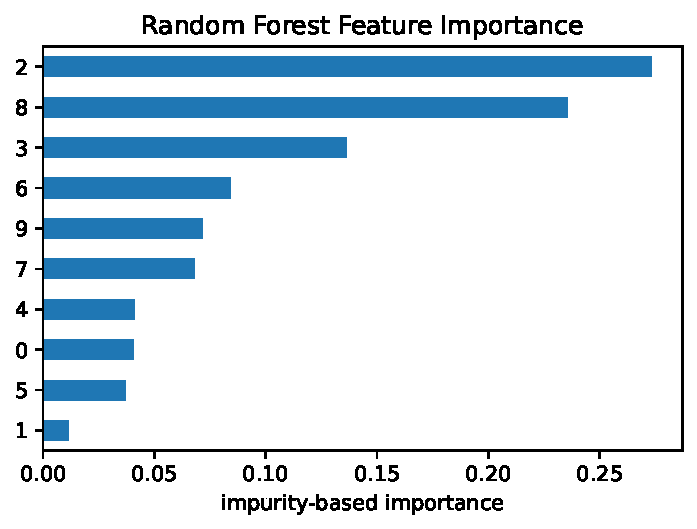
\includegraphics[keepaspectratio]{contents/2/rf_files/figure-pdf/cell-28-output-1.pdf}}

These values measure how much each variable reduces prediction error
inside the trees. They are useful for a quick summary, but they should
not be treated as causal effects.

Permutation importance gives a more direct performance-based measure.

\begin{Shaded}
\begin{Highlighting}[]
\ImportTok{from}\NormalTok{ sklearn.inspection }\ImportTok{import}\NormalTok{ permutation\_importance}

\NormalTok{perm }\OperatorTok{=}\NormalTok{ permutation\_importance(}
\NormalTok{    best\_rf, X\_test, y\_test, n\_repeats}\OperatorTok{=}\DecValTok{30}\NormalTok{, random\_state}\OperatorTok{=}\DecValTok{1}\NormalTok{, n\_jobs}\OperatorTok{={-}}\DecValTok{1}
\NormalTok{)}
\NormalTok{perm\_importance }\OperatorTok{=}\NormalTok{ pd.Series(perm.importances\_mean).sort\_values(ascending}\OperatorTok{=}\VariableTok{True}\NormalTok{)}

\NormalTok{perm\_importance.plot(kind}\OperatorTok{=}\StringTok{"barh"}\NormalTok{)}
\NormalTok{plt.xlabel(}\StringTok{"decrease in R\^{}2 after permutation"}\NormalTok{)}
\NormalTok{plt.title(}\StringTok{"Permutation Importance"}\NormalTok{)}
\end{Highlighting}
\end{Shaded}

\pandocbounded{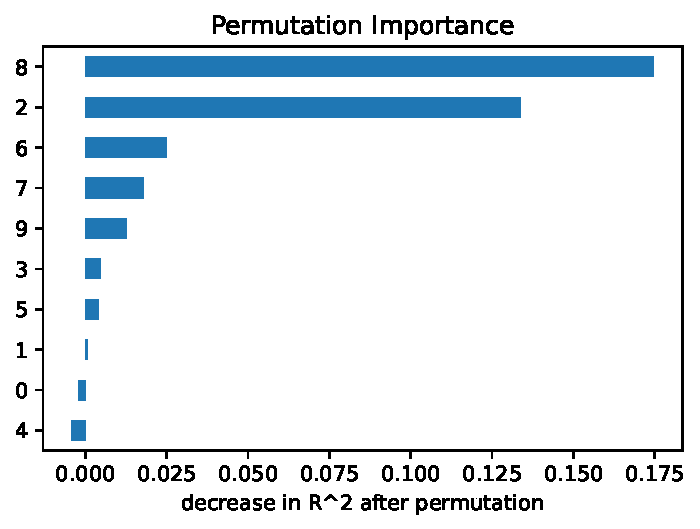
\includegraphics[keepaspectratio]{contents/2/rf_files/figure-pdf/cell-29-output-1.pdf}}

If permuting a predictor substantially worsens predictions, then the
fitted random forest relies on that predictor. If the importance is near
zero, the predictor may not add much predictive information beyond the
others.

From the two plots, feature 2 and 8 are the two most important features.
If we go back to check the description of the dataset, they are
\texttt{bmi:\ body\ mass\ index} and
\texttt{s5:\ ltg,\ possibly\ log\ of\ serum\ triglycerides\ level}.

\chapter{Boosting}\label{boosting}

Boosting is another ensemble method. Like bagging and random forests, it
combines many trees into one model. The difference is how the trees are
built.

Bagging and random forests build trees independently and then average
them.

Boosting builds trees sequentially. Each new tree is trained to improve
the current ensemble.

The central idea is:

\begin{quote}
Build many weak learners one at a time, and let each new learner focus
on what the current model still gets wrong.
\end{quote}

This chapter first discusses AdaBoost. AdaBoost is historically
important and is the cleanest way to see the boosting idea. We then
discuss the margin effect of AdaBoost and how to tune its
hyperparameters. Finally, we discuss gradient boosting and use XGBoost
as the main implementation example.

\section{AdaBoost}\label{adaboost}

AdaBoost (Adaptive Boosting) was introduced by Yoav Freund and Robert E.
Schapire in 1995 {[}10{]} as one of the first highly successful boosting
algorithms. Their original work showed that many weak learners, each
performing only slightly better than random guessing, could be combined
into a highly accurate classifier. AdaBoost became a foundational method
in statistical learning, and it strongly influenced the later
development of modern boosting methods such as Gradient Boosting and
XGBoost.

The original AdaBoost algorithm was proposed as a classification method.
Regression extensions were developed later after the success of AdaBoost
classifiers. In this course, we mainly study AdaBoost classification
because it introduces the core ideas of boosting in a simple and
historically important setting.

For regression problems, we will move on to gradient boosting methods,
which have become the dominant boosting framework in modern machine
learning.

To keep the notation simple, assume the response is binary:

\[
y_i\in\{-1,+1\}.
\]

AdaBoost constructs a classifier of the form

\[
F_M(x)
=
\sum_{m=1}^M \alpha_m G_m(x),
\]

where:

\begin{itemize}
\tightlist
\item
  \(G_m(x)\) is the \(m\)-th weak classifier,
\item
  \(\alpha_m\) is the weight assigned to that classifier,
\item
  \(M\) is the number of boosting rounds.
\end{itemize}

The final prediction is

\[
\hat G(x)
=
\operatorname{sign}\{F_M(x)\}.
\]

Thus AdaBoost is a weighted voting method. Classifiers with larger
\(\alpha_m\) have more influence in the final vote.

\subsection{Weak Learners}\label{weak-learners}

AdaBoost is built from weak learners.

A weak learner is a classifier that is only slightly better than random
guessing. In tree-based AdaBoost, the most common weak learner is a
decision stump, which is a tree with only one split.

In \texttt{sklearn}, a decision stump is created by

\begin{Shaded}
\begin{Highlighting}[]
\ImportTok{from}\NormalTok{ sklearn.tree }\ImportTok{import}\NormalTok{ DecisionTreeClassifier}

\NormalTok{DecisionTreeClassifier(max\_depth}\OperatorTok{=}\DecValTok{1}\NormalTok{)}
\end{Highlighting}
\end{Shaded}

A decision stump is extremely simple and usually underfits when used
alone. One of the most surprising and important ideas behind AdaBoost is
that by combining many such weak learners sequentially, the resulting
ensemble can become a highly accurate and powerful model.

\subsection{Weights of observations}\label{weights-of-observations}

In AdaBoost, there are two different types of weights.

\begin{itemize}
\tightlist
\item
  Estimator weights (\(\alpha_m\)) determine how much influence each
  weak learner has in the final ensemble.
\item
  Observation weights (\(w_i^{(m)}\)) determine which training
  observations receive more attention when fitting the next learner.
\end{itemize}

During training, AdaBoost repeatedly updates the weights of the training
observations. Observations that are difficult to classify receive larger
weights, so future learners focus more on them.

To understand this process, we need to discuss how a decision tree is
trained on a weighted dataset.

The main idea is very simple. In an ordinary dataset, quantities such as
class frequencies and node sample counts are computed using the number
of observations. For a weighted dataset, these counts are replaced by
weighted counts, that is, by the sum of the observation weights.

For example, suppose a node contains observations with weights
\(w_1,w_2,\dots,w_n\). Then the effective sample size of the node
becomes \(\sum_{i=1}^n w_i\). Similarly, class proportions are computed
using weighted proportions rather than ordinary proportions.

Therefore, training a decision tree on weighted data is conceptually
very similar to ordinary tree training. We simply replace ordinary
counts by weighted counts throughout the splitting calculations.

\begin{example}[]\protect\hypertarget{exm-}{}\label{exm-}

Consider the following data:

\begin{longtable}[]{@{}llll@{}}
\caption{}\label{T_cd98c}\tabularnewline
\toprule\noalign{}
x0 & x1 & y & Weight \\
\midrule\noalign{}
\endfirsthead
\toprule\noalign{}
x0 & x1 & y & Weight \\
\midrule\noalign{}
\endhead
\bottomrule\noalign{}
\endlastfoot
1.0 & 2.1 & + & 0.5 \\
1.0 & 1.1 & + & 0.125 \\
1.3 & 1.0 & - & 0.125 \\
1.0 & 1.0 & - & 0.125 \\
2.0 & 1.0 & + & 0.125 \\
\end{longtable}

The weighted Gini impurity is

\[
\text{WeightedGini}=1-(0.5+0.125+0.125)^2-(0.125+0.125)^2=0.375.
\]

\end{example}

\subsection{The AdaBoost Algorithm}\label{the-adaboost-algorithm}

Suppose we have training data

\[
(x_1,y_1),\ldots,(x_n,y_n),
\quad y_i\in\{-1,+1\}.
\]

Initialize observation weights:

\[
w_i^{(1)}=\frac1n.
\]

Then AdaBoost proceeds as follows.

\begin{enumerate}
\def\labelenumi{\arabic{enumi}.}
\item
  For boosting round \(m=1,\ldots,M\), fit a weak classifier \(G_m\)
  using the current weights.
\item
  Compute the weighted classification error by the \(m\)-th classifier:
  \[
  \operatorname{err}_m
  =\frac{\text{the total weights of misclassified observations}}{\text{the total weights}}=
  \frac{
  \sum_{\text{misclassified}} w_i^{(m)}
  }{
  \sum_{\text{all}} w_i^{(m)}
  }.
  \]
\item
  Assign a weight to the weak classifier: \[
  \alpha_m
  =
  \frac12
  \log\qty(\frac{1-\operatorname{err}_m}{\operatorname{err}_m}).
  \]
\item
  Update observation weights and then normalize the weights so they sum
  to one: \[
  w^{(m+1)}_{i}\xleftarrow{\text{normalize}} \hat w_i^{(m+1)}\leftarrow\begin{cases}
  w^{(m)}_i\exp(-\alpha_m)
  &
  \text{if observation $i$ is correctly classified by the $m$th weak learner,}\\
  w_i^{(m)}\exp(\alpha_m)
  &
  \text{if observation $i$ is misclassified by the $m$th weak learner.}
  \end{cases}
  \] that \[
  w^{(m+1)}_{i}
  =
  \frac{\hat w_i^{(m+1)}}{\sum_j \hat w_j^{(m+1)}}.
  \] It is easy to see from the updating rule that AdaBoost puts more
  weight on observations that were misclassified.
\item
  Repeat the above process until the stop conditions are met.
\end{enumerate}

The final model is then \[
F_M(x)
=
\sum_{m=1}^M \alpha_m G_m(x),
\] and the final prediction is \[
\hat G(x)
=
\operatorname{sign}\qty{F_M(x)}.
\]

\begin{tcolorbox}[enhanced jigsaw, arc=.35mm, bottomrule=.15mm, bottomtitle=1mm, breakable, colback=white, colbacktitle=quarto-callout-note-color!10!white, colframe=quarto-callout-note-color-frame, coltitle=black, left=2mm, leftrule=.75mm, opacityback=0, opacitybacktitle=0.6, rightrule=.15mm, title=\textcolor{quarto-callout-note-color}{\faInfo}\hspace{0.5em}{Learning Rate and the \(\frac12\) Factor}, titlerule=0mm, toprule=.15mm, toptitle=1mm]

In the classical AdaBoost derivation, the classifier weight is

\[
\alpha_m
=
\frac12
\log\qty(\frac{1-\operatorname{err}_m}{\operatorname{err}_m}).
\]

In practice, many implementations additionally introduce a learning rate
\(\eta>0\) and use

\[
\alpha_m
=
\eta\cdot
\frac12
\log\qty(\frac{1-\operatorname{err}_m}{\operatorname{err}_m}).
\]

Some textbooks instead write

\[
\alpha_m
=
\eta\cdot
\log\qty(\frac{1-\operatorname{err}_m}{\operatorname{err}_m}),
\]

that is, without the factor \(\frac12\).

This does not fundamentally change the algorithm. The factor \(\frac12\)
can simply be absorbed into the learning rate by replacing \(\eta\) with
\(\eta/2\). Therefore the two formulas differ only by a rescaling of the
step size.

We mainly use the classical form with \(\frac12\) since it naturally
appears in the standard derivation from exponential loss minimization
and margin theory.

The learning rate controls how much each weak learner contributes to the
final ensemble.

\begin{itemize}
\tightlist
\item
  A larger learning rate makes the model change more aggressively at
  each iteration.
\item
  A smaller learning rate produces more gradual updates.
\end{itemize}

In practice, smaller learning rates are often combined with a larger
number of estimators.

\end{tcolorbox}

\begin{tcolorbox}[enhanced jigsaw, arc=.35mm, bottomrule=.15mm, bottomtitle=1mm, breakable, colback=white, colbacktitle=quarto-callout-note-color!10!white, colframe=quarto-callout-note-color-frame, coltitle=black, left=2mm, leftrule=.75mm, opacityback=0, opacitybacktitle=0.6, rightrule=.15mm, title=\textcolor{quarto-callout-note-color}{\faInfo}\hspace{0.5em}{Margin}, titlerule=0mm, toprule=.15mm, toptitle=1mm]

\(yF(x)\) is called the margin of the model \(F\) on the observation
\((x,y)\). Since AdaBoost uses \(\operatorname{sign}\qty{F(x)}\) as the
final prediction rule, the margin can be interpreted as a confidence
score for the prediction.

\begin{itemize}
\tightlist
\item
  If the margin is positive, the prediction is correct.
\item
  If the margin is negative, the prediction is incorrect.
\item
  A larger positive margin indicates a more confident prediction.
\item
  A margin close to zero indicates uncertainty.
\end{itemize}

Notice that the observation weight updating formula can be rewritten as
\[
w_i^{(m+1)}
=
w_i^{(m)}
\exp\qty(-\alpha_m y_i G_m(x_i)),
\] where \(y_i G_m(x_i)\) is exactly the margin of the weak learner
\(G_m\) on observation \((x_i,y_i)\).

Therefore, AdaBoost increases the weights of observations with small or
negative margins and decreases the weights of observations with large
positive margins. In this sense, AdaBoost can be viewed as an algorithm
that attempts to improve the margin distribution by pushing margins
toward larger positive values.

Margin theory is one of the central ideas in boosting and helps explain
why boosting methods often continue to improve test performance even
after the training error has already reached zero. We will discuss this
topic in more detail later.

\end{tcolorbox}

\begin{tcolorbox}[enhanced jigsaw, arc=.35mm, bottomrule=.15mm, bottomtitle=1mm, breakable, colback=white, colbacktitle=quarto-callout-note-color!10!white, colframe=quarto-callout-note-color-frame, coltitle=black, left=2mm, leftrule=.75mm, opacityback=0, opacitybacktitle=0.6, rightrule=.15mm, title=\textcolor{quarto-callout-note-color}{\faInfo}\hspace{0.5em}{Why the Learner Weight Makes Sense}, titlerule=0mm, toprule=.15mm, toptitle=1mm]

The classifier weight is

\[
\alpha_m
=
\eta\cdot\log\left(
\frac{1-\operatorname{err}_m}{\operatorname{err}_m}
\right).
\]

\begin{itemize}
\tightlist
\item
  If \(\operatorname{err}_m\) is small, then the classifier is useful
  and \(\alpha_m\) is large.
\item
  If \(\operatorname{err}_m\) is close to \(0.5\), then the classifier
  is close to random guessing and \(\alpha_m\) is close to zero.
\item
  If \(\operatorname{err}_m>0.5\), then the classifier is worse than
  random guessing. In practice, this means the weak learner is not doing
  its job.
\end{itemize}

\end{tcolorbox}

\subsection{Why Does AdaBoost Work?}\label{why-does-adaboost-work}

One of the most surprising aspects of AdaBoost is that it often performs
extremely well even when each individual learner is very weak.

A useful way to understand boosting is through the bias-variance
tradeoff.

\begin{itemize}
\tightlist
\item
  Bagging and Random Forests mainly reduce variance by averaging many
  trees independently built.
\item
  Boosting mainly reduces bias by sequentially correcting the errors
  made by the current model.
\end{itemize}

At each boosting round, the new learner focuses more on the observations
that are currently difficult to classify. As more learners are added,
many simple decision rules combine into a much more flexible decision
boundary. This sequential correction process allows AdaBoost to
gradually improve the model while still using very simple base learners
such as decision stumps.

In the early boosting rounds, the model often becomes substantially more
accurate. However, if boosting continues too aggressively, variance may
eventually increase and overfitting may occur. Several techniques are
commonly used to control this effect, like shallow trees, smaller
learning rates, subsampling and early stopping. Thus boosting can often
achieve highly accurate models while still maintaining good
generalization performance.

From a mathematical viewpoint, understanding \emph{why} AdaBoost works
so well mathematically became one of the major research topics in
statistical learning during the late 1990s and early 2000s. Many
theoretical studies showed that AdaBoost is closely connected to several
important topics, including additive modeling, exponential loss
minimization and margin theory.

One particularly influential result showed that AdaBoost can be
interpreted as a stagewise additive optimization procedure. Important
theoretical works include {[}11{]}, {[}12{]}, {[}13{]}, and {[}14{]}.
These studies greatly influenced the later development of modern
boosting methods such as Gradient Boosting and XGBoost.

\section{AdaBoost in Python}\label{adaboost-in-python}

The basic APIs are as usual. We use \texttt{AdaBoostClassifier} from
\texttt{sklearn.ensemble} to implement AdaBoost. All the regular APIs
are the same to other models.

\begin{Shaded}
\begin{Highlighting}[]
\ImportTok{from}\NormalTok{ sklearn.tree }\ImportTok{import}\NormalTok{ DecisionTreeClassifier}
\ImportTok{from}\NormalTok{ sklearn.ensemble }\ImportTok{import}\NormalTok{ AdaBoostClassifier}

\NormalTok{ada }\OperatorTok{=}\NormalTok{ AdaBoostClassifier(}
\NormalTok{    estimator}\OperatorTok{=}\NormalTok{DecisionTreeClassifier(max\_depth}\OperatorTok{=}\DecValTok{1}\NormalTok{),}
\NormalTok{    n\_estimators}\OperatorTok{=}\DecValTok{800}\NormalTok{,}
\NormalTok{    learning\_rate}\OperatorTok{=}\FloatTok{0.1}\NormalTok{,}
\NormalTok{    random\_state}\OperatorTok{=}\DecValTok{1}\NormalTok{,}
\NormalTok{)}

\NormalTok{ada.fit(X\_train, y\_train)}
\end{Highlighting}
\end{Shaded}

\begin{tcolorbox}[enhanced jigsaw, arc=.35mm, bottomrule=.15mm, bottomtitle=1mm, breakable, colback=white, colbacktitle=quarto-callout-note-color!10!white, colframe=quarto-callout-note-color-frame, coltitle=black, left=2mm, leftrule=.75mm, opacityback=0, opacitybacktitle=0.6, rightrule=.15mm, title=\textcolor{quarto-callout-note-color}{\faInfo}\hspace{0.5em}{SAMME and SAMME.R}, titlerule=0mm, toprule=.15mm, toptitle=1mm]

The original AdaBoost algorithm was designed for binary classification.
Later extensions such as SAMME and SAMME.R generalized AdaBoost to
multiclass classification problems. In \texttt{sklearn}, multiclass
classification for \texttt{AdaBoostClassifier} is implemented using the
SAMME algorithm by default.

However, these variants are less important in modern statistical
learning practice and will not be studied in detail in this course. One
reason is that these extensions substantially increase the algorithmic
complexity while introducing relatively limited new conceptual ideas
beyond the original AdaBoost framework. In particular, SAMME.R relies
heavily on predicted class probabilities, making the method more
sensitive to the quality of probability estimation and numerical
stability.

More importantly, many of the key ideas behind SAMME.R already overlap
with the additive optimization viewpoint used in modern gradient
boosting methods. As a result, modern frameworks such as Gradient
Boosting and XGBoost provide a more general, flexible, and unified
approach for both regression and classification problems.

Consequently, we will focus primarily on the original AdaBoost
classifier as an accessible introduction to the core ideas of boosting
before moving directly to Gradient Boosting. Reflecting a similar shift
in modern machine learning practice, \texttt{sklearn} has also
deprecated SAMME.R in recent versions due to its reliance on probability
estimation and its conceptual overlap with more general gradient
boosting frameworks.

\end{tcolorbox}

\subsection{The Margin Effect of
AdaBoost}\label{the-margin-effect-of-adaboost}

AdaBoost is often explained as an algorithm that reduces training error.
However, its behavior is more subtle than that.

For a binary classifier with labels \(y_i\in\{-1,+1\}\), define the
margin of observation \(i\) as

\[
\operatorname{margin}_i
=
y_iF_M(x_i).
\]

The sign of the margin determines whether the observation is classified
correctly:

\begin{itemize}
\tightlist
\item
  if \(\operatorname{margin}_i>0\), the observation is correctly
  classified;
\item
  if \(\operatorname{margin}_i<0\), the observation is misclassified.
\end{itemize}

The magnitude of the margin measures confidence. A large positive margin
means the ensemble strongly supports the correct class.

\subsection{Why Margins Matter}\label{why-margins-matter}

AdaBoost often continues to improve test performance even after the
training error has reached zero. This can seem surprising. If the
training error is already zero, what is left to improve?

The answer is margins.

After all training observations are classified correctly, AdaBoost may
still increase the margins. Larger margins mean the classifier is more
confident and more stable. This can improve generalization.

\begin{tcolorbox}[enhanced jigsaw, arc=.35mm, bottomrule=.15mm, bottomtitle=1mm, breakable, colback=white, colbacktitle=quarto-callout-note-color!10!white, colframe=quarto-callout-note-color-frame, coltitle=black, left=2mm, leftrule=.75mm, opacityback=0, opacitybacktitle=0.6, rightrule=.15mm, title=\textcolor{quarto-callout-note-color}{\faInfo}\hspace{0.5em}{Margin view}, titlerule=0mm, toprule=.15mm, toptitle=1mm]

Training error only asks whether the margin is positive.

The margin view also asks how positive it is.

\end{tcolorbox}

This is one reason AdaBoost can work well in practice. It does not only
try to classify points correctly. It also tends to push correctly
classified points farther away from the decision boundary.

\subsection{Margin study in Python}\label{margin-study-in-python}

The following example uses a manually crafted dataset. We track training
error, test error, and margins as the number of boosting rounds
increases.

\begin{Shaded}
\begin{Highlighting}[]
\ImportTok{import}\NormalTok{ numpy }\ImportTok{as}\NormalTok{ np}
\ImportTok{from}\NormalTok{ sklearn.model\_selection }\ImportTok{import}\NormalTok{ train\_test\_split}

\NormalTok{rng }\OperatorTok{=}\NormalTok{ np.random.default\_rng(}\DecValTok{1}\NormalTok{)}

\NormalTok{n }\OperatorTok{=} \DecValTok{3000}
\NormalTok{p }\OperatorTok{=} \DecValTok{10}
\NormalTok{X }\OperatorTok{=}\NormalTok{ rng.normal(size}\OperatorTok{=}\NormalTok{(n, p))}

\NormalTok{score }\OperatorTok{=}\NormalTok{ (}
    \FloatTok{1.2} \OperatorTok{*}\NormalTok{ (X[:, }\DecValTok{0}\NormalTok{] }\OperatorTok{\textgreater{}} \OperatorTok{{-}}\FloatTok{0.6}\NormalTok{)}
    \OperatorTok{+} \FloatTok{1.0} \OperatorTok{*}\NormalTok{ (X[:, }\DecValTok{0}\NormalTok{] }\OperatorTok{\textgreater{}} \FloatTok{0.4}\NormalTok{)}
    \OperatorTok{{-}} \FloatTok{1.1} \OperatorTok{*}\NormalTok{ (X[:, }\DecValTok{1}\NormalTok{] }\OperatorTok{\textgreater{}} \FloatTok{0.0}\NormalTok{)}
    \OperatorTok{+} \FloatTok{0.9} \OperatorTok{*}\NormalTok{ (X[:, }\DecValTok{2}\NormalTok{] }\OperatorTok{\textgreater{}} \FloatTok{0.5}\NormalTok{)}
    \OperatorTok{{-}} \FloatTok{0.8} \OperatorTok{*}\NormalTok{ (X[:, }\DecValTok{3}\NormalTok{] }\OperatorTok{\textgreater{}} \OperatorTok{{-}}\FloatTok{0.2}\NormalTok{)}
    \OperatorTok{+} \FloatTok{0.7} \OperatorTok{*}\NormalTok{ ((X[:, }\DecValTok{4}\NormalTok{] }\OperatorTok{\textgreater{}} \DecValTok{0}\NormalTok{) }\OperatorTok{\&}\NormalTok{ (X[:, }\DecValTok{5}\NormalTok{] }\OperatorTok{\textgreater{}} \DecValTok{0}\NormalTok{))}
    \OperatorTok{{-}} \FloatTok{0.7} \OperatorTok{*}\NormalTok{ ((X[:, }\DecValTok{6}\NormalTok{] }\OperatorTok{\textless{}} \DecValTok{0}\NormalTok{) }\OperatorTok{\&}\NormalTok{ (X[:, }\DecValTok{7}\NormalTok{] }\OperatorTok{\textgreater{}} \FloatTok{0.3}\NormalTok{))}
    \OperatorTok{+} \FloatTok{0.5} \OperatorTok{*}\NormalTok{ (X[:, }\DecValTok{8}\NormalTok{] }\OperatorTok{\textgreater{}} \FloatTok{0.1}\NormalTok{)}
    \OperatorTok{{-}} \FloatTok{0.5} \OperatorTok{*}\NormalTok{ (X[:, }\DecValTok{9}\NormalTok{] }\OperatorTok{\textgreater{}} \OperatorTok{{-}}\FloatTok{0.4}\NormalTok{)}
\NormalTok{)}
\NormalTok{y }\OperatorTok{=} \DecValTok{2} \OperatorTok{*}\NormalTok{ (score }\OperatorTok{\textgreater{}}\NormalTok{ np.quantile(score, }\FloatTok{0.52}\NormalTok{)).astype(}\BuiltInTok{int}\NormalTok{) }\OperatorTok{{-}} \DecValTok{1}

\NormalTok{X\_train, X\_test, y\_train, y\_test }\OperatorTok{=}\NormalTok{ train\_test\_split(}
\NormalTok{    X, y, test\_size}\OperatorTok{=}\FloatTok{0.5}\NormalTok{, stratify}\OperatorTok{=}\NormalTok{y, random\_state}\OperatorTok{=}\DecValTok{1}
\NormalTok{)}
\end{Highlighting}
\end{Shaded}

We first train the model.

\begin{Shaded}
\begin{Highlighting}[]
\ImportTok{from}\NormalTok{ sklearn.tree }\ImportTok{import}\NormalTok{ DecisionTreeClassifier}
\ImportTok{from}\NormalTok{ sklearn.ensemble }\ImportTok{import}\NormalTok{ AdaBoostClassifier}

\NormalTok{ada }\OperatorTok{=}\NormalTok{ AdaBoostClassifier(}
\NormalTok{    estimator}\OperatorTok{=}\NormalTok{DecisionTreeClassifier(max\_depth}\OperatorTok{=}\DecValTok{2}\NormalTok{, random\_state}\OperatorTok{=}\DecValTok{1}\NormalTok{),}
\NormalTok{    n\_estimators}\OperatorTok{=}\DecValTok{2000}\NormalTok{,}
\NormalTok{    learning\_rate}\OperatorTok{=}\FloatTok{0.2}\NormalTok{,}
\NormalTok{    random\_state}\OperatorTok{=}\DecValTok{1}\NormalTok{,}
\NormalTok{)}

\NormalTok{ada.fit(X\_train, y\_train)}
\end{Highlighting}
\end{Shaded}

{\def\LTcaptype{none} % do not increment counter
\begin{longtable}[]{@{}
  >{\raggedright\arraybackslash}p{(\linewidth - 4\tabcolsep) * \real{0.3333}}
  >{\raggedright\arraybackslash}p{(\linewidth - 4\tabcolsep) * \real{0.3333}}
  >{\raggedright\arraybackslash}p{(\linewidth - 4\tabcolsep) * \real{0.3333}}@{}}
\toprule\noalign{}
\endhead
\bottomrule\noalign{}
\endlastfoot
\emph{} & \begin{minipage}[t]{\linewidth}\raggedright
\href{https://scikit-learn.org/1.8/modules/generated/sklearn.ensemble.AdaBoostClassifier.html\#:~:text=estimator,-object\%2C\%20default\%3DNone}{estimator
{estimator: object, default=None\\
\strut \\
The base estimator from which the boosted ensemble is built.\\
Support for sample weighting is required, as well as proper\\
``classes\_`` and ``n\_classes\_`` attributes. If ``None``, then\\
the base estimator is
:class:`\textasciitilde sklearn.tree.DecisionTreeClassifier`\\
initialized with `max\_depth=1`.\\
\strut \\
.. versionadded:: 1.2\\
`base\_estimator` was renamed to `estimator`.}}\strut
\end{minipage} & DecisionTreeC...andom\_state=1) \\
\emph{} & \begin{minipage}[t]{\linewidth}\raggedright
\href{https://scikit-learn.org/1.8/modules/generated/sklearn.ensemble.AdaBoostClassifier.html\#:~:text=n_estimators,-int\%2C\%20default\%3D50}{n\_estimators
{n\_estimators: int, default=50\\
\strut \\
The maximum number of estimators at which boosting is terminated.\\
In case of perfect fit, the learning procedure is stopped early.\\
Values must be in the range `{[}1, inf)`.}}\strut
\end{minipage} & 2000 \\
\emph{} & \begin{minipage}[t]{\linewidth}\raggedright
\href{https://scikit-learn.org/1.8/modules/generated/sklearn.ensemble.AdaBoostClassifier.html\#:~:text=learning_rate,-float\%2C\%20default\%3D1.0}{learning\_rate
{learning\_rate: float, default=1.0\\
\strut \\
Weight applied to each classifier at each boosting iteration. A higher\\
learning rate increases the contribution of each classifier. There is\\
a trade-off between the `learning\_rate` and `n\_estimators`
parameters.\\
Values must be in the range `(0.0, inf)`.}}\strut
\end{minipage} & 0.2 \\
\emph{} & \begin{minipage}[t]{\linewidth}\raggedright
\href{https://scikit-learn.org/1.8/modules/generated/sklearn.ensemble.AdaBoostClassifier.html\#:~:text=random_state,-int\%2C\%20RandomState\%20instance\%20or\%20None\%2C\%20default\%3DNone}{random\_state
{random\_state: int, RandomState instance or None, default=None\\
\strut \\
Controls the random seed given at each `estimator` at each\\
boosting iteration.\\
Thus, it is only used when `estimator` exposes a `random\_state`.\\
Pass an int for reproducible output across multiple function calls.\\
See :term:`Glossary `.}}\strut
\end{minipage} & 1 \\
\end{longtable}
}

{\def\LTcaptype{none} % do not increment counter
\begin{longtable}[]{@{}
  >{\raggedright\arraybackslash}p{(\linewidth - 4\tabcolsep) * \real{0.3333}}
  >{\raggedright\arraybackslash}p{(\linewidth - 4\tabcolsep) * \real{0.3333}}
  >{\raggedright\arraybackslash}p{(\linewidth - 4\tabcolsep) * \real{0.3333}}@{}}
\toprule\noalign{}
\endhead
\bottomrule\noalign{}
\endlastfoot
\emph{} & \begin{minipage}[t]{\linewidth}\raggedright
\href{https://scikit-learn.org/1.8/modules/generated/sklearn.tree.DecisionTreeClassifier.html\#:~:text=criterion,-\%7B\%22gini\%22\%2C\%20\%22entropy\%22\%2C\%20\%22log_loss\%22\%7D\%2C\%20default\%3D\%22gini\%22}{criterion
{criterion: \{"gini", "entropy", "log\_loss"\}, default="gini"\\
\strut \\
The function to measure the quality of a split. Supported criteria are\\
"gini" for the Gini impurity and "log\_loss" and "entropy" both for
the\\
Shannon information gain, see
:ref:`tree\_mathematical\_formulation`.}}\strut
\end{minipage} & \textquotesingle gini\textquotesingle{} \\
\emph{} & \begin{minipage}[t]{\linewidth}\raggedright
\href{https://scikit-learn.org/1.8/modules/generated/sklearn.tree.DecisionTreeClassifier.html\#:~:text=splitter,-\%7B\%22best\%22\%2C\%20\%22random\%22\%7D\%2C\%20default\%3D\%22best\%22}{splitter
{splitter: \{"best", "random"\}, default="best"\\
\strut \\
The strategy used to choose the split at each node. Supported\\
strategies are "best" to choose the best split and "random" to choose\\
the best random split.}}\strut
\end{minipage} & \textquotesingle best\textquotesingle{} \\
\emph{} & \begin{minipage}[t]{\linewidth}\raggedright
\href{https://scikit-learn.org/1.8/modules/generated/sklearn.tree.DecisionTreeClassifier.html\#:~:text=max_depth,-int\%2C\%20default\%3DNone}{max\_depth
{max\_depth: int, default=None\\
\strut \\
The maximum depth of the tree. If None, then nodes are expanded until\\
all leaves are pure or until all leaves contain less than\\
min\_samples\_split samples.}}\strut
\end{minipage} & 2 \\
\emph{} & \begin{minipage}[t]{\linewidth}\raggedright
\href{https://scikit-learn.org/1.8/modules/generated/sklearn.tree.DecisionTreeClassifier.html\#:~:text=min_samples_split,-int\%20or\%20float\%2C\%20default\%3D2}{min\_samples\_split
{min\_samples\_split: int or float, default=2\\
\strut \\
The minimum number of samples required to split an internal node:\\
\strut \\
- If int, then consider `min\_samples\_split` as the minimum number.\\
- If float, then `min\_samples\_split` is a fraction and\\
`ceil(min\_samples\_split * n\_samples)` are the minimum\\
number of samples for each split.\\
\strut \\
.. versionchanged:: 0.18\\
Added float values for fractions.}}\strut
\end{minipage} & 2 \\
\emph{} & \begin{minipage}[t]{\linewidth}\raggedright
\href{https://scikit-learn.org/1.8/modules/generated/sklearn.tree.DecisionTreeClassifier.html\#:~:text=min_samples_leaf,-int\%20or\%20float\%2C\%20default\%3D1}{min\_samples\_leaf
{min\_samples\_leaf: int or float, default=1\\
\strut \\
The minimum number of samples required to be at a leaf node.\\
A split point at any depth will only be considered if it leaves at\\
least ``min\_samples\_leaf`` training samples in each of the left and\\
right branches. This may have the effect of smoothing the model,\\
especially in regression.\\
\strut \\
- If int, then consider `min\_samples\_leaf` as the minimum number.\\
- If float, then `min\_samples\_leaf` is a fraction and\\
`ceil(min\_samples\_leaf * n\_samples)` are the minimum\\
number of samples for each node.\\
\strut \\
.. versionchanged:: 0.18\\
Added float values for fractions.}}\strut
\end{minipage} & 1 \\
\emph{} & \begin{minipage}[t]{\linewidth}\raggedright
\href{https://scikit-learn.org/1.8/modules/generated/sklearn.tree.DecisionTreeClassifier.html\#:~:text=min_weight_fraction_leaf,-float\%2C\%20default\%3D0.0}{min\_weight\_fraction\_leaf
{min\_weight\_fraction\_leaf: float, default=0.0\\
\strut \\
The minimum weighted fraction of the sum total of weights (of all\\
the input samples) required to be at a leaf node. Samples have\\
equal weight when sample\_weight is not provided.}}\strut
\end{minipage} & 0.0 \\
\emph{} & \begin{minipage}[t]{\linewidth}\raggedright
\href{https://scikit-learn.org/1.8/modules/generated/sklearn.tree.DecisionTreeClassifier.html\#:~:text=max_features,-int\%2C\%20float\%20or\%20\%7B\%22sqrt\%22\%2C\%20\%22log2\%22\%7D\%2C\%20default\%3DNone}{max\_features
{max\_features: int, float or \{"sqrt", "log2"\}, default=None\\
\strut \\
The number of features to consider when looking for the best split:\\
\strut \\
- If int, then consider `max\_features` features at each split.\\
- If float, then `max\_features` is a fraction and\\
`max(1, int(max\_features * n\_features\_in\_))` features are considered
at\\
each split.\\
- If "sqrt", then `max\_features=sqrt(n\_features)`.\\
- If "log2", then `max\_features=log2(n\_features)`.\\
- If None, then `max\_features=n\_features`.\\
\strut \\
.. note::\\
\strut \\
The search for a split does not stop until at least one\\
valid partition of the node samples is found, even if it requires to\\
effectively inspect more than ``max\_features`` features.}}\strut
\end{minipage} & None \\
\emph{} & \begin{minipage}[t]{\linewidth}\raggedright
\href{https://scikit-learn.org/1.8/modules/generated/sklearn.tree.DecisionTreeClassifier.html\#:~:text=random_state,-int\%2C\%20RandomState\%20instance\%20or\%20None\%2C\%20default\%3DNone}{random\_state
{random\_state: int, RandomState instance or None, default=None\\
\strut \\
Controls the randomness of the estimator. The features are always\\
randomly permuted at each split, even if ``splitter`` is set to\\
``"best"``. When ``max\_features \textless{} n\_features``, the
algorithm will\\
select ``max\_features`` at random at each split before finding the
best\\
split among them. But the best found split may vary across different\\
runs, even if ``max\_features=n\_features``. That is the case, if the\\
improvement of the criterion is identical for several splits and one\\
split has to be selected at random. To obtain a deterministic
behaviour\\
during fitting, ``random\_state`` has to be fixed to an integer.\\
See :term:`Glossary ` for details.}}\strut
\end{minipage} & 1 \\
\emph{} & \begin{minipage}[t]{\linewidth}\raggedright
\href{https://scikit-learn.org/1.8/modules/generated/sklearn.tree.DecisionTreeClassifier.html\#:~:text=max_leaf_nodes,-int\%2C\%20default\%3DNone}{max\_leaf\_nodes
{max\_leaf\_nodes: int, default=None\\
\strut \\
Grow a tree with ``max\_leaf\_nodes`` in best-first fashion.\\
Best nodes are defined as relative reduction in impurity.\\
If None then unlimited number of leaf nodes.}}\strut
\end{minipage} & None \\
\emph{} & \begin{minipage}[t]{\linewidth}\raggedright
\href{https://scikit-learn.org/1.8/modules/generated/sklearn.tree.DecisionTreeClassifier.html\#:~:text=min_impurity_decrease,-float\%2C\%20default\%3D0.0}{min\_impurity\_decrease
{min\_impurity\_decrease: float, default=0.0\\
\strut \\
A node will be split if this split induces a decrease of the impurity\\
greater than or equal to this value.\\
\strut \\
The weighted impurity decrease equation is the following::\\
\strut \\
N\_t / N * (impurity - N\_t\_R / N\_t * right\_impurity\\
- N\_t\_L / N\_t * left\_impurity)\\
\strut \\
where ``N`` is the total number of samples, ``N\_t`` is the number of\\
samples at the current node, ``N\_t\_L`` is the number of samples in
the\\
left child, and ``N\_t\_R`` is the number of samples in the right
child.\\
\strut \\
``N``, ``N\_t``, ``N\_t\_R`` and ``N\_t\_L`` all refer to the weighted
sum,\\
if ``sample\_weight`` is passed.\\
\strut \\
.. versionadded:: 0.19}}\strut
\end{minipage} & 0.0 \\
\emph{} & \begin{minipage}[t]{\linewidth}\raggedright
\href{https://scikit-learn.org/1.8/modules/generated/sklearn.tree.DecisionTreeClassifier.html\#:~:text=class_weight,-dict\%2C\%20list\%20of\%20dict\%20or\%20\%22balanced\%22\%2C\%20default\%3DNone}{class\_weight
{class\_weight: dict, list of dict or "balanced", default=None\\
\strut \\
Weights associated with classes in the form ``\{class\_label:
weight\}``.\\
If None, all classes are supposed to have weight one. For\\
multi-output problems, a list of dicts can be provided in the same\\
order as the columns of y.\\
\strut \\
Note that for multioutput (including multilabel) weights should be\\
defined for each class of every column in its own dict. For example,\\
for four-class multilabel classification weights should be\\
{[}\{0: 1, 1: 1\}, \{0: 1, 1: 5\}, \{0: 1, 1: 1\}, \{0: 1, 1: 1\}{]}
instead of\\
{[}\{1:1\}, \{2:5\}, \{3:1\}, \{4:1\}{]}.\\
\strut \\
The "balanced" mode uses the values of y to automatically adjust\\
weights inversely proportional to class frequencies in the input data\\
as ``n\_samples / (n\_classes * np.bincount(y))``\\
\strut \\
For multi-output, the weights of each column of y will be multiplied.\\
\strut \\
Note that these weights will be multiplied with sample\_weight (passed\\
through the fit method) if sample\_weight is specified.}}\strut
\end{minipage} & None \\
\emph{} & \begin{minipage}[t]{\linewidth}\raggedright
\href{https://scikit-learn.org/1.8/modules/generated/sklearn.tree.DecisionTreeClassifier.html\#:~:text=ccp_alpha,-non-negative\%20float\%2C\%20default\%3D0.0}{ccp\_alpha
{ccp\_alpha: non-negative float, default=0.0\\
\strut \\
Complexity parameter used for Minimal Cost-Complexity Pruning. The\\
subtree with the largest cost complexity that is smaller than\\
``ccp\_alpha`` will be chosen. By default, no pruning is performed.
See\\
:ref:`minimal\_cost\_complexity\_pruning` for details. See\\
:ref:`sphx\_glr\_auto\_examples\_tree\_plot\_cost\_complexity\_pruning.py`\\
for an example of such pruning.\\
\strut \\
.. versionadded:: 0.22}}\strut
\end{minipage} & 0.0 \\
\emph{} & \begin{minipage}[t]{\linewidth}\raggedright
\href{https://scikit-learn.org/1.8/modules/generated/sklearn.tree.DecisionTreeClassifier.html\#:~:text=monotonic_cst,-array-like\%20of\%20int\%20of\%20shape\%20\%28n_features\%29\%2C\%20default\%3DNone}{monotonic\_cst
{monotonic\_cst: array-like of int of shape (n\_features),
default=None\\
\strut \\
Indicates the monotonicity constraint to enforce on each feature.\\
- 1: monotonic increase\\
- 0: no constraint\\
- -1: monotonic decrease\\
\strut \\
If monotonic\_cst is None, no constraints are applied.\\
\strut \\
Monotonicity constraints are not supported for:\\
- multiclass classifications (i.e. when `n\_classes \textgreater{}
2`),\\
- multioutput classifications (i.e. when `n\_outputs\_ \textgreater{}
1`),\\
- classifications trained on data with missing values.\\
\strut \\
The constraints hold over the probability of the positive class.\\
\strut \\
Read more in the :ref:`User Guide `.\\
\strut \\
.. versionadded:: 1.4}}\strut
\end{minipage} & None \\
\end{longtable}
}

Then since the model contains the information of all trees, we could
directly read them and use them about how the model works if we only use
the first several trees. Here we use \texttt{.staged\_predict()} and
\texttt{.staged\_decision\_function()} methods.

\begin{itemize}
\tightlist
\item
  \texttt{.staged\_predict()}: returns the predictions after each
  boosting round.
\item
  \texttt{.staged\_decision\_function()}: returns the decision scores
  after each boosting round.
\end{itemize}

We would like to record all the training and test scores.

\begin{Shaded}
\begin{Highlighting}[]
\ImportTok{from}\NormalTok{ sklearn.metrics }\ImportTok{import}\NormalTok{ accuracy\_score}

\NormalTok{train\_acc }\OperatorTok{=}\NormalTok{ []}
\NormalTok{test\_acc }\OperatorTok{=}\NormalTok{ []}

\ControlFlowTok{for}\NormalTok{ pred\_train, pred\_test }\KeywordTok{in} \BuiltInTok{zip}\NormalTok{(}
\NormalTok{    ada.staged\_predict(X\_train), ada.staged\_predict(X\_test)}
\NormalTok{):}
\NormalTok{    train\_acc.append(accuracy\_score(y\_train, pred\_train))}
\NormalTok{    test\_acc.append(accuracy\_score(y\_test, pred\_test))}
\end{Highlighting}
\end{Shaded}

In addition, the 10th-percentile margin is of our interesting, since we
treat margin\textless10\% as no confidence.

\begin{Shaded}
\begin{Highlighting}[]
\NormalTok{train\_margin\_10 }\OperatorTok{=}\NormalTok{ []}
\NormalTok{test\_margin\_10 }\OperatorTok{=}\NormalTok{ []}

\ControlFlowTok{for}\NormalTok{ score\_train, score\_test }\KeywordTok{in} \BuiltInTok{zip}\NormalTok{(}
\NormalTok{    ada.staged\_decision\_function(X\_train),}
\NormalTok{    ada.staged\_decision\_function(X\_test),}
\NormalTok{):}
\NormalTok{    train\_margins }\OperatorTok{=}\NormalTok{ y\_train }\OperatorTok{*}\NormalTok{ score\_train}
\NormalTok{    test\_margins }\OperatorTok{=}\NormalTok{ y\_test }\OperatorTok{*}\NormalTok{ score\_test}

\NormalTok{    train\_margin\_10.append(np.quantile(train\_margins, }\FloatTok{0.1}\NormalTok{))}
\NormalTok{    test\_margin\_10.append(np.quantile(test\_margins, }\FloatTok{0.1}\NormalTok{))}
\end{Highlighting}
\end{Shaded}

We also need to test when the training score becomes \texttt{1.0}, and
when the test score is the highest. Then we have the interesting output.

\begin{Shaded}
\begin{Highlighting}[]
\NormalTok{first\_full\_train }\OperatorTok{=} \BuiltInTok{next}\NormalTok{((i }\OperatorTok{+} \DecValTok{1} \ControlFlowTok{for}\NormalTok{ i, s }\KeywordTok{in} \BuiltInTok{enumerate}\NormalTok{(train\_acc) }\ControlFlowTok{if}\NormalTok{ s }\OperatorTok{==} \FloatTok{1.0}\NormalTok{), }\VariableTok{None}\NormalTok{)}
\NormalTok{best\_test\_round }\OperatorTok{=}\NormalTok{ np.argmax(test\_acc) }\OperatorTok{+} \DecValTok{1}

\BuiltInTok{print}\NormalTok{(}\StringTok{"First round with training accuracy 1:"}\NormalTok{, first\_full\_train)}
\BuiltInTok{print}\NormalTok{(}\StringTok{"Test accuracy at that round:"}\NormalTok{, test\_acc[first\_full\_train }\OperatorTok{{-}} \DecValTok{1}\NormalTok{])}
\BuiltInTok{print}\NormalTok{(}\StringTok{"Best test accuracy:"}\NormalTok{, np.}\BuiltInTok{max}\NormalTok{(test\_acc))}
\BuiltInTok{print}\NormalTok{(}\StringTok{"Best test round:"}\NormalTok{, best\_test\_round)}
\BuiltInTok{print}\NormalTok{(}\StringTok{"Final training accuracy:"}\NormalTok{, train\_acc[}\OperatorTok{{-}}\DecValTok{1}\NormalTok{])}
\BuiltInTok{print}\NormalTok{(}\StringTok{"Final test accuracy:"}\NormalTok{, test\_acc[}\OperatorTok{{-}}\DecValTok{1}\NormalTok{])}
\end{Highlighting}
\end{Shaded}

\begin{verbatim}
First round with training accuracy 1: 426
Test accuracy at that round: 0.9746666666666667
Best test accuracy: 0.9806666666666667
Best test round: 1121
Final training accuracy: 1.0
Final test accuracy: 0.98
\end{verbatim}

We could plot the curves. From the plot, we can see that after the
training score becomes 1.0, the model is still improving and the test
score reaches the highest long after.

\begin{Shaded}
\begin{Highlighting}[]
\ImportTok{import}\NormalTok{ matplotlib.pyplot }\ImportTok{as}\NormalTok{ plt}

\NormalTok{plt.plot(train\_acc, label}\OperatorTok{=}\StringTok{"training accuracy"}\NormalTok{)}
\NormalTok{plt.plot(test\_acc, label}\OperatorTok{=}\StringTok{"testing accuracy"}\NormalTok{)}

\NormalTok{plt.axvline(}
\NormalTok{    first\_full\_train,}
\NormalTok{    color}\OperatorTok{=}\StringTok{"black"}\NormalTok{,}
\NormalTok{    linestyle}\OperatorTok{=}\StringTok{"{-}{-}"}\NormalTok{,}
\NormalTok{    label}\OperatorTok{=}\StringTok{"training accuracy first reaches 1"}\NormalTok{,}
\NormalTok{)}

\NormalTok{plt.axvline(best\_test\_round, color}\OperatorTok{=}\StringTok{"gray"}\NormalTok{, linestyle}\OperatorTok{=}\StringTok{":"}\NormalTok{, label}\OperatorTok{=}\StringTok{"best testing accuracy"}\NormalTok{)}

\NormalTok{plt.xlabel(}\StringTok{"boosting round"}\NormalTok{)}
\NormalTok{plt.ylabel(}\StringTok{"accuracy"}\NormalTok{)}
\NormalTok{plt.title(}\StringTok{"Accuracy Curves"}\NormalTok{)}
\NormalTok{plt.legend()}\OperatorTok{;}
\end{Highlighting}
\end{Shaded}

\pandocbounded{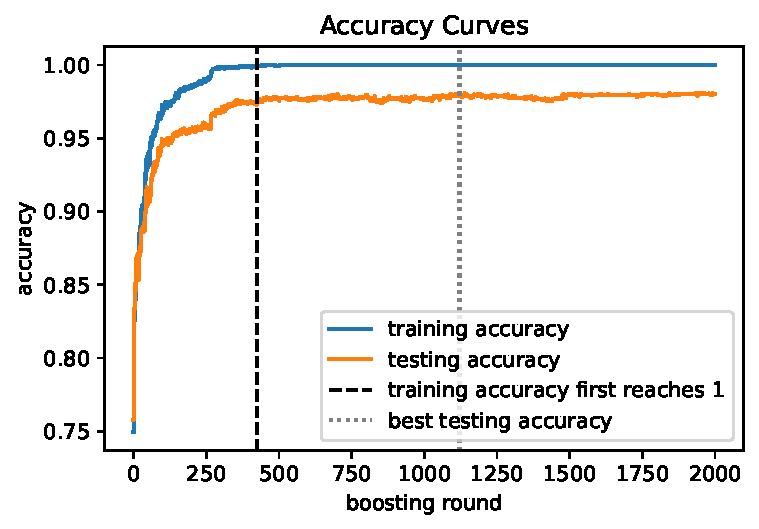
\includegraphics[keepaspectratio]{contents/2/boost_files/figure-pdf/cell-10-output-1.pdf}}

We may also plot the 10th-percentile margin curve. The 10th-percentile
margin represents the lower tail of the margin distribution, that is,
the examples on which the classifier is least confident.

From the plot, we can see that even after the training accuracy reaches
1.0, the margins may still continue to change. This shows that
\texttt{AdaBoost} is not merely optimizing training accuracy; it
continues to adjust the additive model in order to improve the margin
distribution and increase confidence.

\begin{itemize}
\tightlist
\item
  If the lower-percentile margin continues to increase while test
  performance remains stable or improves, this suggests that the model
  is still improving its confidence on difficult cases and is not yet
  clearly overfitting.
\item
  If the lower-percentile margin decreases together with decreasing
  validation or test performance, this suggests that the model may be
  becoming less reliable on difficult cases and may be starting to
  overfit.
\end{itemize}

\begin{Shaded}
\begin{Highlighting}[]
\NormalTok{plt.plot(train\_margin\_10, label}\OperatorTok{=}\StringTok{"training 10th percentile margin"}\NormalTok{)}
\NormalTok{plt.plot(test\_margin\_10, label}\OperatorTok{=}\StringTok{"testing 10th percentile margin"}\NormalTok{)}

\NormalTok{plt.axvline(}
\NormalTok{    first\_full\_train,}
\NormalTok{    color}\OperatorTok{=}\StringTok{"black"}\NormalTok{,}
\NormalTok{    linestyle}\OperatorTok{=}\StringTok{"{-}{-}"}\NormalTok{,}
\NormalTok{    label}\OperatorTok{=}\StringTok{"training accuracy first reaches 1"}\NormalTok{,}
\NormalTok{)}

\NormalTok{plt.axhline(}\DecValTok{0}\NormalTok{, color}\OperatorTok{=}\StringTok{"black"}\NormalTok{, linewidth}\OperatorTok{=}\DecValTok{1}\NormalTok{)}

\NormalTok{plt.xlabel(}\StringTok{"boosting round"}\NormalTok{)}
\NormalTok{plt.ylabel(}\StringTok{"margin"}\NormalTok{)}
\NormalTok{plt.title(}\StringTok{"10th Percentile Margin"}\NormalTok{)}
\NormalTok{plt.legend()}\OperatorTok{;}
\end{Highlighting}
\end{Shaded}

\pandocbounded{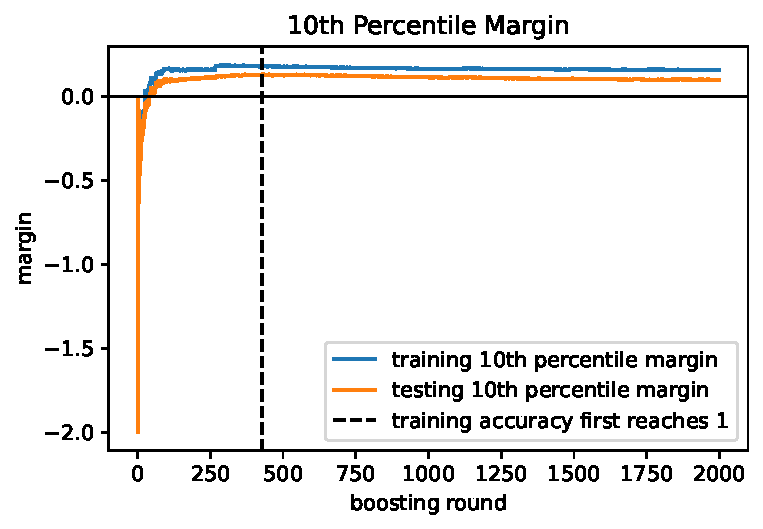
\includegraphics[keepaspectratio]{contents/2/boost_files/figure-pdf/cell-11-output-1.pdf}}

\section{Tuning AdaBoost
Hyperparameters}\label{tuning-adaboost-hyperparameters}

The most important AdaBoost hyperparameters are:

{\def\LTcaptype{none} % do not increment counter
\begin{longtable}[]{@{}ll@{}}
\toprule\noalign{}
Parameter & Role \\
\midrule\noalign{}
\endhead
\bottomrule\noalign{}
\endlastfoot
\texttt{n\_estimators} & Number of weak learners. \\
\texttt{learning\_rate} & Shrinks the contribution of each learner. \\
\texttt{estimator\_\_max\_depth} & Complexity of the base tree. \\
\texttt{estimator\_\_min\_samples\_leaf} & Smoothness of each base
tree. \\
\end{longtable}
}

The two most important parameters are \texttt{n\_estimators} and
\texttt{learning\_rate}.

\subsection{Learning Rate and Number of
Trees}\label{learning-rate-and-number-of-trees}

There is a strong tradeoff:

\begin{itemize}
\tightlist
\item
  smaller \texttt{learning\_rate} usually needs larger
  \texttt{n\_estimators};
\item
  larger \texttt{learning\_rate} learns faster but can overfit or become
  unstable;
\item
  smaller \texttt{learning\_rate} often gives smoother and more stable
  models.
\end{itemize}

\subsection{Base Tree Depth}\label{base-tree-depth}

Decision stumps use \texttt{max\_depth=1}. They are common because
AdaBoost was originally designed around weak learners. Using deeper
trees allows each boosting round to model interactions. In most cases,
AdaBoost use depths from 1 to 3. Deeper trees are stronger learners, but
they also increase the risk of overfitting.

\subsection{Grid Search for AdaBoost}\label{grid-search-for-adaboost}

The following code tunes AdaBoost by grid search cross-validation.

\begin{Shaded}
\begin{Highlighting}[]
\ImportTok{from}\NormalTok{ sklearn.model\_selection }\ImportTok{import}\NormalTok{ GridSearchCV}
\ImportTok{from}\NormalTok{ sklearn.tree }\ImportTok{import}\NormalTok{ DecisionTreeClassifier}
\ImportTok{from}\NormalTok{ sklearn.ensemble }\ImportTok{import}\NormalTok{ AdaBoostClassifier}

\NormalTok{ada }\OperatorTok{=}\NormalTok{ AdaBoostClassifier(}
\NormalTok{    estimator}\OperatorTok{=}\NormalTok{DecisionTreeClassifier(random\_state}\OperatorTok{=}\DecValTok{0}\NormalTok{),}
\NormalTok{    random\_state}\OperatorTok{=}\DecValTok{0}\NormalTok{,}
\NormalTok{)}

\NormalTok{param\_grid }\OperatorTok{=}\NormalTok{ \{}
    \StringTok{"n\_estimators"}\NormalTok{: [}\DecValTok{100}\NormalTok{, }\DecValTok{300}\NormalTok{, }\DecValTok{600}\NormalTok{],}
    \StringTok{"learning\_rate"}\NormalTok{: [}\FloatTok{0.01}\NormalTok{, }\FloatTok{0.05}\NormalTok{, }\FloatTok{0.1}\NormalTok{, }\FloatTok{0.5}\NormalTok{],}
    \StringTok{"estimator\_\_max\_depth"}\NormalTok{: [}\DecValTok{1}\NormalTok{, }\DecValTok{2}\NormalTok{, }\DecValTok{3}\NormalTok{],}
    \StringTok{"estimator\_\_min\_samples\_leaf"}\NormalTok{: [}\DecValTok{1}\NormalTok{, }\DecValTok{5}\NormalTok{, }\DecValTok{10}\NormalTok{],}
\NormalTok{\}}

\NormalTok{grid }\OperatorTok{=}\NormalTok{ GridSearchCV(ada, param\_grid}\OperatorTok{=}\NormalTok{param\_grid, cv}\OperatorTok{=}\DecValTok{5}\NormalTok{, scoring}\OperatorTok{=}\StringTok{"accuracy"}\NormalTok{, n\_jobs}\OperatorTok{={-}}\DecValTok{1}\NormalTok{)}

\NormalTok{grid.fit(X\_train, y\_train)}
\NormalTok{grid.best\_params\_}
\end{Highlighting}
\end{Shaded}

Tuning should be done using validation data or cross-validation. The
test set should be saved for the final evaluation.

\begin{tcolorbox}[enhanced jigsaw, arc=.35mm, bottomrule=.15mm, bottomtitle=1mm, breakable, colback=white, colbacktitle=quarto-callout-caution-color!10!white, colframe=quarto-callout-caution-color-frame, coltitle=black, left=2mm, leftrule=.75mm, opacityback=0, opacitybacktitle=0.6, rightrule=.15mm, title=\textcolor{quarto-callout-caution-color}{\faFire}\hspace{0.5em}{Noisy data}, titlerule=0mm, toprule=.15mm, toptitle=1mm]

AdaBoost can be sensitive to mislabeled observations and outliers.

Because it repeatedly increases the weights of difficult observations,
noisy points may receive too much attention.

\end{tcolorbox}

\subsection{\texorpdfstring{Example: \texttt{AdaBoost} on a Nonlinear
Classification
Problem}{Example: AdaBoost on a Nonlinear Classification Problem}}\label{example-adaboost-on-a-nonlinear-classification-problem}

We first use a synthetic nonlinear classification problem. This example
shows that many weak learners can create a flexible decision boundary.

\begin{Shaded}
\begin{Highlighting}[]
\ImportTok{from}\NormalTok{ sklearn.datasets }\ImportTok{import}\NormalTok{ make\_moons}
\ImportTok{from}\NormalTok{ sklearn.model\_selection }\ImportTok{import}\NormalTok{ train\_test\_split}

\NormalTok{X, y }\OperatorTok{=}\NormalTok{ make\_moons(n\_samples}\OperatorTok{=}\DecValTok{1500}\NormalTok{, noise}\OperatorTok{=}\FloatTok{0.25}\NormalTok{, random\_state}\OperatorTok{=}\DecValTok{1}\NormalTok{)}

\NormalTok{X\_train, X\_test, y\_train, y\_test }\OperatorTok{=}\NormalTok{ train\_test\_split(}
\NormalTok{    X, y, test\_size}\OperatorTok{=}\FloatTok{0.3}\NormalTok{, stratify}\OperatorTok{=}\NormalTok{y, random\_state}\OperatorTok{=}\DecValTok{1}
\NormalTok{)}
\end{Highlighting}
\end{Shaded}

Fit a baseline stump and an AdaBoost model.

\begin{Shaded}
\begin{Highlighting}[]
\ImportTok{from}\NormalTok{ sklearn.tree }\ImportTok{import}\NormalTok{ DecisionTreeClassifier}
\ImportTok{from}\NormalTok{ sklearn.ensemble }\ImportTok{import}\NormalTok{ AdaBoostClassifier}

\NormalTok{stump }\OperatorTok{=}\NormalTok{ DecisionTreeClassifier(max\_depth}\OperatorTok{=}\DecValTok{1}\NormalTok{, random\_state}\OperatorTok{=}\DecValTok{1}\NormalTok{)}

\NormalTok{ada }\OperatorTok{=}\NormalTok{ AdaBoostClassifier(}
\NormalTok{    estimator}\OperatorTok{=}\NormalTok{DecisionTreeClassifier(max\_depth}\OperatorTok{=}\DecValTok{1}\NormalTok{, random\_state}\OperatorTok{=}\DecValTok{1}\NormalTok{),}
\NormalTok{    n\_estimators}\OperatorTok{=}\DecValTok{300}\NormalTok{,}
\NormalTok{    learning\_rate}\OperatorTok{=}\FloatTok{0.05}\NormalTok{,}
\NormalTok{    random\_state}\OperatorTok{=}\DecValTok{1}\NormalTok{,}
\NormalTok{)}

\NormalTok{stump.fit(X\_train, y\_train)}
\NormalTok{ada.fit(X\_train, y\_train)}

\BuiltInTok{print}\NormalTok{(}\StringTok{"Stump accuracy:"}\NormalTok{, stump.score(X\_test, y\_test))}
\BuiltInTok{print}\NormalTok{(}\StringTok{"AdaBoost accuracy:"}\NormalTok{, ada.score(X\_test, y\_test))}
\end{Highlighting}
\end{Shaded}

\begin{verbatim}
Stump accuracy: 0.8488888888888889
AdaBoost accuracy: 0.9222222222222223
\end{verbatim}

Now tune the AdaBoost model.

\begin{Shaded}
\begin{Highlighting}[]
\ImportTok{from}\NormalTok{ sklearn.model\_selection }\ImportTok{import}\NormalTok{ GridSearchCV}
\ImportTok{from}\NormalTok{ sklearn.metrics }\ImportTok{import}\NormalTok{ accuracy\_score}

\NormalTok{ada\_base }\OperatorTok{=}\NormalTok{ AdaBoostClassifier(}
\NormalTok{    estimator}\OperatorTok{=}\NormalTok{DecisionTreeClassifier(random\_state}\OperatorTok{=}\DecValTok{1}\NormalTok{), random\_state}\OperatorTok{=}\DecValTok{1}
\NormalTok{)}

\NormalTok{param\_grid }\OperatorTok{=}\NormalTok{ \{}
    \StringTok{"n\_estimators"}\NormalTok{: [}\DecValTok{100}\NormalTok{, }\DecValTok{300}\NormalTok{, }\DecValTok{600}\NormalTok{],}
    \StringTok{"learning\_rate"}\NormalTok{: [}\FloatTok{0.03}\NormalTok{, }\FloatTok{0.05}\NormalTok{, }\FloatTok{0.1}\NormalTok{],}
    \StringTok{"estimator\_\_max\_depth"}\NormalTok{: [}\DecValTok{1}\NormalTok{, }\DecValTok{2}\NormalTok{],}
    \StringTok{"estimator\_\_min\_samples\_leaf"}\NormalTok{: [}\DecValTok{1}\NormalTok{, }\DecValTok{5}\NormalTok{],}
\NormalTok{\}}

\NormalTok{grid }\OperatorTok{=}\NormalTok{ GridSearchCV(}
\NormalTok{    ada\_base, param\_grid}\OperatorTok{=}\NormalTok{param\_grid, cv}\OperatorTok{=}\DecValTok{5}\NormalTok{, scoring}\OperatorTok{=}\StringTok{"accuracy"}\NormalTok{, n\_jobs}\OperatorTok{={-}}\DecValTok{1}
\NormalTok{)}

\NormalTok{grid.fit(X\_train, y\_train)}
\NormalTok{best\_ada }\OperatorTok{=}\NormalTok{ grid.best\_estimator\_}

\BuiltInTok{print}\NormalTok{(}\StringTok{"Best parameters:"}\NormalTok{, grid.best\_params\_)}
\BuiltInTok{print}\NormalTok{(}\StringTok{"Best CV accuracy:"}\NormalTok{, grid.best\_score\_)}
\BuiltInTok{print}\NormalTok{(}\StringTok{"Test accuracy:"}\NormalTok{, best\_ada.score(X\_test, y\_test))}
\end{Highlighting}
\end{Shaded}

\begin{verbatim}
Best parameters: {'estimator__max_depth': 2, 'estimator__min_samples_leaf': 5, 'learning_rate': 0.1, 'n_estimators': 600}
Best CV accuracy: 0.9466666666666667
Test accuracy: 0.94
\end{verbatim}

\section{XGBoost and Gradient
Boosting}\label{xgboost-and-gradient-boosting}

The core idea of boosting is to sequentially train models in order to
correct the errors made by earlier models. A natural idea is therefore:

\begin{enumerate}
\def\labelenumi{\arabic{enumi}.}
\tightlist
\item
  fit a model
\item
  compute the residuals
\item
  fit a new model to the residuals
\item
  repeat
\end{enumerate}

We mainly consider regression problems at the current stage.

\subsection{Additive model}\label{additive-model}

The above idea leads directly to \textbf{Gradient Boosting}. When the
models used are trees, the model is also called Gradient Boosted
Decision Trees (GBDT).

Gradient Boosting builds an additive model of the form

\[
F_M(x) = \sum_{m=1}^M \beta_m h_m(x)
\]

where

\begin{itemize}
\tightlist
\item
  \(h_m(x)\) is usually a small regression tree
\item
  \(\beta_m\) is a coefficient
\item
  the model is built sequentially
\end{itemize}

Unlike bagging, where trees are trained independently, boosting trains
each new tree based on the current errors of the model.

\subsection{Functional gradient
viewpoint}\label{functional-gradient-viewpoint}

In ordinary optimization problems, we optimize finitely many parameters.
For example, in linear regression we optimize the coefficient vector

\[
\beta=(\beta_1,\ldots,\beta_p).
\]

Gradient Boosting takes a different viewpoint. Instead of directly
optimizing finitely many parameters, it attempts to optimize the
prediction function itself.

The model is built additively:

\[
F_{m+1}(x)
=
F_m(x)+f_m(x),
\]

where each new function \(f_m(x)\) is usually a small regression tree.

Thus each boosting step adds a new basis function to the model. Since
the space of possible functions is extremely large, Gradient Boosting is
often interpreted as a form of gradient descent in function space, also
called functional gradient descent.

Conceptually:

\begin{itemize}
\tightlist
\item
  ordinary gradient descent updates parameters
\item
  Gradient Boosting updates functions
\end{itemize}

\subsection{Regression tree fitting}\label{regression-tree-fitting}

In order to find the best model \(F(x)\), we would like to minimize the
empirical loss function

\[
L(F)=\sum_{i=1}^n l(y_i,F(x_i)),
\]

where \(\{(x_i,y_i)\}\) is the training dataset. One of the most common
choices for the loss function is the squared-error loss \[
L(F)
=
\sum_{i=1}^n
(y_i-F(x_i))^2.
\]

Assume the current model is \(F_m(x)\). After adding a new tree
\(f_m(x)\), the next model becomes

\[
F_{m+1}(x)
=
F_m(x)+f_m(x).
\]

The new tree \(f_m(x)\) is chosen to reduce the loss function. Ideally,
we would minimize \[
l(y_i,F_m(x_i)+f_m(x_i))
\] for each \(f_m(x_i)\). Gradient boosting approximates this
optimization using the idea of gradient descent: the predictions
\(f_m(x_i)\) should approximate the negative gradient, which gives the
direction of steepest descent in the loss. We therefore define the
pseudo-residual for the observation \(x_i\) as

\[
r_i
=-g_i
=
-
\left.
\frac{\partial l(y_i,F(x_i))}
{\partial F(x_i)}
\right|_{F=F_m}.
\] The pseudo-residuals \(r_i\) are then used as the target values when
fitting the new regression tree \(f_m\).

Assume that the new tree splits the dataset into regions
\(R_1,\ldots,R_s\), and for each region \(R_j\) a value \(s_j\) is
assigned. We would like the tree to approximate the pseudo-residuals
\(r_i\). Therefore we choose the tree to minimize

\[
\sum_{j=1}^s
\sum_{x_i\in R_j}
(r_i-s_j)^2.
\]

For a fixed region \(R_j\), the optimal value of \(s_j\) is the mean of
the observations inside that region:

\[
s_j
=
\frac{1}{|R_j|}
\sum_{x_i\in R_j} r_i.
\]

Therefore, the new tree \(f_m(x)\) is simply a regression tree (trained
using RSS) with target values \(r_i\).

\begin{tcolorbox}[enhanced jigsaw, arc=.35mm, bottomrule=.15mm, bottomtitle=1mm, breakable, colback=white, colbacktitle=quarto-callout-note-color!10!white, colframe=quarto-callout-note-color-frame, coltitle=black, left=2mm, leftrule=.75mm, opacityback=0, opacitybacktitle=0.6, rightrule=.15mm, title=\textcolor{quarto-callout-note-color}{\faInfo}\hspace{0.5em}{Pseudo-residual}, titlerule=0mm, toprule=.15mm, toptitle=1mm]

\(r_i\) is called a \emph{pseudo-residual} because it is technically a
negative gradient rather than an ordinary residual. However, it plays
the role of the residual in Gradient Boosting.

For squared-error loss

\[
l(y,F(x))
=
(y-F(x))^2,
\]

we have

\[
r_i
=
2(y_i-F_m(x_i)),
\]

which is proportional to the ordinary residual.

Therefore, under \(L^2\) loss, Gradient Boosting can literally be
interpreted as fitting residuals.

\end{tcolorbox}

\subsection{XGBoost: Initial idea}\label{xgboost-initial-idea}

XGBoost stands for \textbf{Extreme Gradient Boosting}. Its mathematical
foundation can be viewed as a modified and improved version of GBDT.

XGBoost became one of the most successful shallow machine learning
models in modern practice. In addition to its mathematical improvements,
it also introduced many engineering innovations that significantly
improved efficiency and scalability. After the success of XGBoost,
several related models such as LightGBM and CatBoost were also developed
and became widely used.

We mainly focus on the mathematical ideas behind XGBoost. The motivation
is very similar to GBDT. We consider the additive model

\[
F_{m+1}(x)
=
F_m(x)+f_m(x),
\]

and would like to minimize the empirical loss

\[
L(F)
=
\sum_{i=1}^n l(y_i,F(x_i)).
\]

Assume the current model is \(F_m(x)\). After adding a new tree
\(f_m(x)\), we obtain

\[
F_{m+1}(x)
=
F_m(x)+f_m(x).
\]

Instead of using only first-order information as in GBDT, XGBoost uses a
local second-order Taylor approximation of the loss function at each
boosting iteration:

\begin{equation}\protect\phantomsection\label{eq-xg_loss}{
l(y_i,F_m(x_i)+f_m(x_i))
\approx
l(y_i,F_m(x_i))
+
g_i f_m(x_i)
+
\frac12 h_i f_m(x_i)^2,
}\end{equation}

where

\[
g_i
=
\left.
\frac{\partial l(y_i,F(x_i))}
{\partial F(x_i)}
\right|_{F=F_m},
\]

and

\[
h_i
=
\left.
\frac{\partial^2 l(y_i,F(x_i))}
{\partial F(x_i)^2}
\right|_{F=F_m}.
\]

Here

\begin{itemize}
\tightlist
\item
  \(g_i\) measures the gradient
\item
  \(h_i\) measures the curvature of the loss function
\end{itemize}

Thus, XGBoost uses both gradient and curvature information.

\subsection{Tree structure in XGBoost}\label{tree-structure-in-xgboost}

Assume that the new tree splits the dataset into regions

\[
R_1,\ldots,R_s,
\]

and assigns a prediction value \(s_j\) to region \(R_j\). Then for every
observation inside region \(R_j\), we have

\[
f_m(x_i)=s_j.
\]

Substituting this into the quadratic approximation
Equation~\ref{eq-xg_loss} and ignoring constant terms gives the
approximate objective

\[
\sum_{j=1}^s
\sum_{x_i\in R_j}
\left(
g_i s_j
+
\frac12 h_i s_j^2
\right).
\]

For a fixed tree structure, we minimize this expression with respect to
\(s_j\).

Differentiating with respect to \(s_j\) gives

\[
\sum_{x_i\in R_j}
(g_i+h_i s_j)
=
0.
\]

Therefore,

\[
s_j
=
-
\frac{
\sum_{x_i\in R_j} g_i
}{
\sum_{x_i\in R_j} h_i
}.
\]

If we define

\[
G_j
=
\sum_{x_i\in R_j} g_i,
\quad
H_j
=
\sum_{x_i\in R_j} h_i,
\]

then the optimal leaf value becomes

\[
s_j
=
-\frac{G_j}{H_j}.
\]

\begin{tcolorbox}[enhanced jigsaw, arc=.35mm, bottomrule=.15mm, bottomtitle=1mm, breakable, colback=white, colbacktitle=quarto-callout-warning-color!10!white, colframe=quarto-callout-warning-color-frame, coltitle=black, left=2mm, leftrule=.75mm, opacityback=0, opacitybacktitle=0.6, rightrule=.15mm, title=\textcolor{quarto-callout-warning-color}{\faExclamationTriangle}\hspace{0.5em}{Important difference from ordinary CART}, titlerule=0mm, toprule=.15mm, toptitle=1mm]

This tree is NOT an ordinary CART regression tree trained with RSS.

\begin{itemize}
\tightlist
\item
  In GBDT, we explicitly train a CART regression tree to fit the
  pseudo-residuals.
\item
  In XGBoost, the leaf values are derived directly from the quadratic
  approximation of the objective function itself.
\end{itemize}

Therefore, although XGBoost trees may look structurally similar to CART
trees, mathematically they are solving a different optimization problem.

\end{tcolorbox}

\subsection{Regularization}\label{regularization-2}

So far we derived the basic XGBoost objective using the second-order
Taylor approximation.

However, minimizing only the training loss may produce overly complex
trees and lead to overfitting. Therefore XGBoost introduces an explicit
regularization term to control tree complexity.

Suppose the new tree \(f_m(x)\) has

\begin{itemize}
\tightlist
\item
  \(T\) leaves
\item
  leaf values \(s_1,\ldots,s_T\)
\end{itemize}

XGBoost defines the regularization term

\[
\Omega(f_m)
=
\gamma T
+
\frac12 \lambda \sum_{j=1}^T s_j^2.
\]

Therefore the objective becomes

\[
L(F_m+f_m)
+
\Omega(f_m).
\]

\begin{itemize}
\tightlist
\item
  \(\gamma T\) penalizes the number of leaves. The parameter \(\gamma\),
  called the minimum split loss, specifies the minimum reduction in the
  objective required for an additional split.
\item
  \(\frac{1}{2}\lambda\sum_{j=1}^{T}s_j^2\) penalizes large leaf
  weights. The parameter \(\lambda\) controls the strength of this
  \(L_2\) regularization.
\end{itemize}

Using the second-order Taylor approximation and grouping terms by
regions gives

\[
\sum_{j=1}^T
\left[
G_j s_j
+
\frac12 (H_j+\lambda)s_j^2
\right]
+
\gamma T.
\]

For a fixed tree structure, we minimize the objective with respect to
\(s_j\). Differentiating gives

\[
G_j+(H_j+\lambda)s_j=0.
\]

Therefore the optimal leaf value becomes

\[
s_j
=
-
\frac{G_j}{H_j+\lambda}.
\]

Compared with the non-regularized version

\[
s_j
=
-\frac{G_j}{H_j},
\]

the regularization term enlarges the denominator and shrinks the leaf
predictions toward zero. This effect is similar to ridge regularization
in linear regression.

Substituting the optimal leaf values back into the objective gives

\[
-\frac12
\sum_{j=1}^T
\frac{G_j^2}{H_j+\lambda}
+
\gamma T.
\]

This quantity is used by XGBoost to evaluate the quality of candidate
tree splits.

Therefore, unlike ordinary CART trees which use RSS or Gini impurity,
XGBoost derives its splitting criterion directly from the regularized
optimization objective.

\begin{tcolorbox}[enhanced jigsaw, arc=.35mm, bottomrule=.15mm, bottomtitle=1mm, breakable, colback=white, colbacktitle=quarto-callout-note-color!10!white, colframe=quarto-callout-note-color-frame, coltitle=black, left=2mm, leftrule=.75mm, opacityback=0, opacitybacktitle=0.6, rightrule=.15mm, title=\textcolor{quarto-callout-note-color}{\faInfo}\hspace{0.5em}{\(L_1\) regularization}, titlerule=0mm, toprule=.15mm, toptitle=1mm]

XGBoost can also apply an \(L_1\) penalty to the leaf weights:

\[
\alpha\sum_{j=1}^{T}|s_j|.
\]

Including both \(L_1\) and \(L_2\) regularization, the full penalty
function becomes

\[
\Omega(f_m)
=
\gamma T
+
\frac{\lambda}{2}\sum_{j=1}^{T}s_j^2
+
\alpha\sum_{j=1}^{T}|s_j|.
\]

The \(L_1\) penalty can shrink some leaf weights exactly to zero, making
the contribution of those leaves vanish. It may improve robustness and
reduce overfitting, particularly when the data contain substantial
noise.

This penalty is analogous to the \(L_1\) penalty used in lasso
regression. However, unlike lasso regression, it regularizes leaf values
rather than individual feature coefficients, so it does not directly
perform feature selection.

We initially omit \(L_1\) regularization because its
nondifferentiability at zero makes the derivation of the optimal leaf
weights and split gains more complicated. Nevertheless, \(\alpha\) is a
hyperparameter worth considering when tuning an \texttt{XGBoost} model.

\end{tcolorbox}

\subsection{Learning rate}\label{learning-rate}

In practice, although XGBoost computes the best update tree \(f_m\), it
usually does not add the full tree update directly to the model.
Instead, the update is scaled by a learning rate (also called the
shrinkage parameter):

\[
F_{m+1}(x)
=
F_m(x)
+
\eta f_m(x),
\]

where

\[
0<\eta\le 1.
\]

Thus every new tree contributes only partially to the final model.

Equivalently, after computing the optimal leaf value

\[
s_j
=
-
\frac{G_j}{H_j+\lambda},
\]

XGBoost actually uses the scaled leaf prediction

\[
\eta s_j.
\]

Therefore shrinkage reduces the influence of each individual tree.

The parameter \(\eta\) is called the \textbf{learning rate} or shrinkage
parameter.

\begin{tcolorbox}[enhanced jigsaw, arc=.35mm, bottomrule=.15mm, bottomtitle=1mm, breakable, colback=white, colbacktitle=quarto-callout-note-color!10!white, colframe=quarto-callout-note-color-frame, coltitle=black, left=2mm, leftrule=.75mm, opacityback=0, opacitybacktitle=0.6, rightrule=.15mm, title=\textcolor{quarto-callout-note-color}{\faInfo}\hspace{0.5em}{XGBoost in practice}, titlerule=0mm, toprule=.15mm, toptitle=1mm]

The mathematical foundation of XGBoost is built on three main ideas:

\begin{itemize}
\tightlist
\item
  second-order Taylor approximation of the loss function
\item
  explicit regularization on tree complexity
\item
  shrinkage through the learning rate
\end{itemize}

In addition to these mathematical ideas, XGBoost also introduced many
important engineering optimizations such as:

\begin{itemize}
\tightlist
\item
  parallel tree construction
\item
  efficient handling of sparse data
\item
  cache-aware memory access
\item
  approximate split finding algorithms
\end{itemize}

These engineering improvements are one of the main reasons why XGBoost
became highly successful in practical machine learning applications.

\end{tcolorbox}

\subsection{GBDT and XGBoost for
classification}\label{gbdt-and-xgboost-for-classification}

Both GBDT and XGBoost can naturally be extended from regression to
classification problems. The overall framework remains the same:

\begin{itemize}
\tightlist
\item
  additive tree model
\item
  boosting optimization
\item
  sequentially adding trees
\item
  minimizing a loss function
\end{itemize}

The main difference is the choice of the loss function.

For binary classification, boosting methods commonly use logistic loss

\[
l(y,p)
=
-
\left[
y\log p+(1-y)\log(1-p)
\right].
\]

The model output \(F(x)\) is converted into probabilities using the
logistic function \[
p(x)
=
\frac1{1+e^{-F(x)}}.
\] For multiclass classification, softmax-based loss functions are
commonly used.

The difference between GBDT and XGBoost remains the same as in
regression:

\begin{itemize}
\tightlist
\item
  GBDT uses first-order gradients (pseudo-residuals)
\item
  XGBoost uses second-order Taylor approximation together with
  regularization
\end{itemize}

Thus both methods provide a unified framework for regression and
classification problems.

\begin{tcolorbox}[enhanced jigsaw, arc=.35mm, bottomrule=.15mm, bottomtitle=1mm, breakable, colback=white, colbacktitle=quarto-callout-note-color!10!white, colframe=quarto-callout-note-color-frame, coltitle=black, left=2mm, leftrule=.75mm, opacityback=0, opacitybacktitle=0.6, rightrule=.15mm, title=\textcolor{quarto-callout-note-color}{\faInfo}\hspace{0.5em}{AdaBoost as Gradient Boosting with exponential loss}, titlerule=0mm, toprule=.15mm, toptitle=1mm]

AdaBoost can be interpreted as a special case of Gradient Boosting using
the exponential loss function

\[
l(y,F(x))
=
e^{-yF(x)},
\]

where

\[
y\in\{-1,1\}.
\]

The empirical loss becomes

\[
L(F)
=
\sum_{i=1}^n
e^{-y_iF(x_i)}.
\]

This loss heavily penalizes observations with negative margins

\[
y_iF(x_i).
\]

In particular:

\begin{itemize}
\tightlist
\item
  correctly classified points with large positive margins receive very
  small loss
\item
  misclassified points receive exponentially large loss
\end{itemize}

Therefore minimizing exponential loss naturally increases the weights of
difficult observations, which explains the adaptive reweighting behavior
of AdaBoost.

Taking derivative gives

\[
\frac{\partial l(y_i,F(x_i))}
{\partial F(x_i)}
=
-y_i e^{-y_iF(x_i)}.
\]

Thus the pseudo-residual becomes

\[
r_i
=
y_i e^{-y_iF(x_i)}.
\]

Observations with small or negative margins receive much larger
pseudo-residuals and therefore larger influence in the next boosting
step.

From this viewpoint, AdaBoost can be interpreted as functional gradient
descent under exponential loss.

Gradient Boosting generalizes this idea by allowing arbitrary
differentiable loss functions rather than only exponential loss.

\end{tcolorbox}

\section{XGBoost in Python}\label{xgboost-in-python}

XGBoost is implemented using the library \texttt{XGBoost}. You may go to
the \href{https://xgboost.ai/}{offical website} for more information. We
will cover the basic usage in this lecture.

A typical XGBoost regression model looks like this.

\begin{Shaded}
\begin{Highlighting}[]
\ImportTok{from}\NormalTok{ xgboost }\ImportTok{import}\NormalTok{ XGBRegressor}

\NormalTok{xgb }\OperatorTok{=}\NormalTok{ XGBRegressor(}
\NormalTok{    objective}\OperatorTok{=}\StringTok{"reg:squarederror"}\NormalTok{,}
\NormalTok{    n\_estimators}\OperatorTok{=}\DecValTok{500}\NormalTok{,}
\NormalTok{    learning\_rate}\OperatorTok{=}\FloatTok{0.05}\NormalTok{,}
\NormalTok{    max\_depth}\OperatorTok{=}\DecValTok{3}\NormalTok{,}
\NormalTok{    subsample}\OperatorTok{=}\FloatTok{0.8}\NormalTok{,}
\NormalTok{    colsample\_bytree}\OperatorTok{=}\FloatTok{0.8}\NormalTok{,}
\NormalTok{    gamma}\OperatorTok{=}\FloatTok{0.5}\NormalTok{,}
\NormalTok{    reg\_lambda}\OperatorTok{=}\FloatTok{1.0}\NormalTok{,}
\NormalTok{    random\_state}\OperatorTok{=}\DecValTok{0}\NormalTok{,}
\NormalTok{    n\_jobs}\OperatorTok{={-}}\DecValTok{1}\NormalTok{,}
\NormalTok{)}

\NormalTok{xgb.fit(X\_train, y\_train)}
\end{Highlighting}
\end{Shaded}

The \texttt{objective="reg:squarederror"} is to indicate the loss
function. The default is \texttt{"reg:squarederror"} that is regression
with squared loss. More loss function can be found in the
\href{https://xgboost.readthedocs.io/en/stable/parameter.html\#learning-task-parameters}{documnet}.

The most important hyperparameters are:

{\def\LTcaptype{none} % do not increment counter
\begin{longtable}[]{@{}ll@{}}
\toprule\noalign{}
Parameter & Meaning \\
\midrule\noalign{}
\endhead
\bottomrule\noalign{}
\endlastfoot
\texttt{n\_estimators} & Number of boosting rounds. \\
\texttt{learning\_rate} & Learning rate. \\
\texttt{max\_depth} & Depth of each tree. \\
\texttt{subsample} & Fraction of observations used for each tree. \\
\texttt{colsample\_bytree} & Fraction of predictors used for each
tree. \\
\texttt{gamma} & Minimum split loss for the tree. \\
\texttt{reg\_lambda} & L2 regularization on leaf weights. \\
\texttt{reg\_alpha} & L1 regularization on leaf weights. \\
\end{longtable}
}

Most of them are straightforward. I only discuss these since they are
not from the theory.

\begin{tcolorbox}[enhanced jigsaw, arc=.35mm, bottomrule=.15mm, bottomtitle=1mm, breakable, colback=white, colbacktitle=quarto-callout-note-color!10!white, colframe=quarto-callout-note-color-frame, coltitle=black, left=2mm, leftrule=.75mm, opacityback=0, opacitybacktitle=0.6, rightrule=.15mm, title=\textcolor{quarto-callout-note-color}{\faInfo}\hspace{0.5em}{\texttt{subsample}}, titlerule=0mm, toprule=.15mm, toptitle=1mm]

\texttt{subsample} controls the fraction of training observations
randomly sampled. For example \texttt{subsample=0.8} means that each new
tree is trained using only 80\% of the observations. Sampling is
performed without replacement, and a new sample is drawn for each
boosting round.

This introduces additional randomness into boosting, similar to bagging
in Random Forests. Smaller values of \texttt{subsample} and reduce
variance and improve generalization. However, if the value is too small,
the model may underfit.

\end{tcolorbox}

\begin{tcolorbox}[enhanced jigsaw, arc=.35mm, bottomrule=.15mm, bottomtitle=1mm, breakable, colback=white, colbacktitle=quarto-callout-note-color!10!white, colframe=quarto-callout-note-color-frame, coltitle=black, left=2mm, leftrule=.75mm, opacityback=0, opacitybacktitle=0.6, rightrule=.15mm, title=\textcolor{quarto-callout-note-color}{\faInfo}\hspace{0.5em}{\texttt{colsample\_bytree}}, titlerule=0mm, toprule=.15mm, toptitle=1mm]

\texttt{colsample\_bytree} controls the fraction of predictors randomly
sampled for each tree. For example \texttt{colsample\_bytree=0.7} means
that each tree only considers 70\% of the predictors. Sampling is
performed without replacement, and a new set of predictors is drawn for
each tree.

This idea is similar to feature subsampling in Random Forests. It
reduces correlation between trees and can improve robustness and
generalization performance. However, Random Forests commonly sample
predictors separately at each split, whereas \texttt{colsample\_bytree}
selects one set of predictors for the entire tree (and therefore its
name is \texttt{bytree}).

\end{tcolorbox}

Example grid:

\begin{Shaded}
\begin{Highlighting}[]
\ImportTok{from}\NormalTok{ sklearn.model\_selection }\ImportTok{import}\NormalTok{ GridSearchCV}
\ImportTok{from}\NormalTok{ xgboost }\ImportTok{import}\NormalTok{ XGBRegressor}

\NormalTok{xgb }\OperatorTok{=}\NormalTok{ XGBRegressor(random\_state}\OperatorTok{=}\DecValTok{1}\NormalTok{, n\_jobs}\OperatorTok{=}\DecValTok{1}\NormalTok{)}

\NormalTok{param\_grid }\OperatorTok{=}\NormalTok{ \{}
    \StringTok{"n\_estimators"}\NormalTok{: [}\DecValTok{200}\NormalTok{, }\DecValTok{500}\NormalTok{, }\DecValTok{800}\NormalTok{],}
    \StringTok{"learning\_rate"}\NormalTok{: [}\FloatTok{0.03}\NormalTok{, }\FloatTok{0.05}\NormalTok{, }\FloatTok{0.1}\NormalTok{],}
    \StringTok{"max\_depth"}\NormalTok{: [}\DecValTok{2}\NormalTok{, }\DecValTok{3}\NormalTok{, }\DecValTok{4}\NormalTok{],}
    \StringTok{"subsample"}\NormalTok{: [}\FloatTok{0.7}\NormalTok{, }\FloatTok{0.9}\NormalTok{, }\FloatTok{1.0}\NormalTok{],}
    \StringTok{"colsample\_bytree"}\NormalTok{: [}\FloatTok{0.7}\NormalTok{, }\FloatTok{0.9}\NormalTok{, }\FloatTok{1.0}\NormalTok{],}
    \StringTok{"gamma"}\NormalTok{: [}\DecValTok{0}\NormalTok{, }\FloatTok{0.01}\NormalTok{, }\FloatTok{0.1}\NormalTok{, }\FloatTok{0.5}\NormalTok{, }\DecValTok{1}\NormalTok{, }\DecValTok{5}\NormalTok{],}
    \StringTok{"reg\_lambda"}\NormalTok{: [}\FloatTok{1.0}\NormalTok{, }\FloatTok{5.0}\NormalTok{, }\FloatTok{10.0}\NormalTok{],}
    \StringTok{"reg\_alpha"}\NormalTok{: [}\DecValTok{0}\NormalTok{, }\FloatTok{0.001}\NormalTok{, }\FloatTok{0.01}\NormalTok{, }\FloatTok{0.1}\NormalTok{, }\DecValTok{1}\NormalTok{, }\DecValTok{5}\NormalTok{, }\DecValTok{10}\NormalTok{],}
\NormalTok{\}}

\NormalTok{grid }\OperatorTok{=}\NormalTok{ GridSearchCV(xgb, param\_grid}\OperatorTok{=}\NormalTok{param\_grid, cv}\OperatorTok{=}\DecValTok{5}\NormalTok{, n\_jobs}\OperatorTok{={-}}\DecValTok{1}\NormalTok{)}

\NormalTok{grid.fit(X\_train, y\_train)}
\end{Highlighting}
\end{Shaded}

\begin{tcolorbox}[enhanced jigsaw, arc=.35mm, bottomrule=.15mm, bottomtitle=1mm, breakable, colback=white, colbacktitle=quarto-callout-note-color!10!white, colframe=quarto-callout-note-color-frame, coltitle=black, left=2mm, leftrule=.75mm, opacityback=0, opacitybacktitle=0.6, rightrule=.15mm, title=\textcolor{quarto-callout-note-color}{\faInfo}\hspace{0.5em}{\texttt{n\_jobs}}, titlerule=0mm, toprule=.15mm, toptitle=1mm]

Although for boosting parallel computing is in the nature as in bagging,
\texttt{XGBoost} successfully support it and offers \texttt{n\_jobs} to
accelerate. The API is similar, so we could use \texttt{n\_jobs=-1} to
indicate using all CPU cores.

Similar to \texttt{bagging}, for a nested structure such as
\texttt{GridSearchCV} with \texttt{XGBoost}, we normally use multiple
cores only at the outermost layer, that is, \texttt{GridSearchCV}.
However, some studies suggest enabling multicore processing in
\texttt{XGBoost} while using a single core for \texttt{GridSearchCV}
when the dataset is very large.

\end{tcolorbox}

\section{Tuning XGBoost}\label{tuning-xgboost}

If there are enough computing resources, to tune \texttt{XGBoost} is no
different from other models. However since the model becomes more
complicated, it usually takes longer to go through the whole grid
search. In this case, usually we make some modifications to the
workflow.

\subsection{\texorpdfstring{\texttt{RandomizedSearchCV}}{RandomizedSearchCV}}\label{randomizedsearchcv}

We already show the code of \texttt{RandomizedSearchCV} before. Here we
give more explanations.

\texttt{RandomizedSearchCV} is to search random combinations of
hyperparameters. Therefore it is used to do a rough search in a very
large parameter space. Other than the \texttt{param\_grid} like
\texttt{GridSearchCV}, \texttt{RandomizedSearchCV} needs
\texttt{n\_iter} to indicate how many combinations one wants to test.

Since now we can search in a very large space, usually we make a really
large space, by directly choosing hyperparameters based on
distributions. We use distributions from the library
\texttt{scipy.stats}. Here we give an examples.

\begin{Shaded}
\begin{Highlighting}[]
\ImportTok{from}\NormalTok{ scipy.stats }\ImportTok{import}\NormalTok{ randint, uniform, loguniform}
\ImportTok{from}\NormalTok{ sklearn.model\_selection }\ImportTok{import}\NormalTok{ RandomizedSearchCV}

\NormalTok{param\_distributions }\OperatorTok{=}\NormalTok{ \{}
    \StringTok{"n\_estimators"}\NormalTok{: randint(}\DecValTok{100}\NormalTok{, }\DecValTok{1000}\NormalTok{),}
    \StringTok{"max\_depth"}\NormalTok{: randint(}\DecValTok{2}\NormalTok{, }\DecValTok{8}\NormalTok{),}
    \StringTok{"learning\_rate"}\NormalTok{: uniform(}\FloatTok{0.01}\NormalTok{, }\FloatTok{0.19}\NormalTok{),}
    \StringTok{"subsample"}\NormalTok{: uniform(}\FloatTok{0.6}\NormalTok{, }\FloatTok{0.4}\NormalTok{),}
    \StringTok{"colsample\_bytree"}\NormalTok{: uniform(}\FloatTok{0.6}\NormalTok{, }\FloatTok{0.4}\NormalTok{),}
    \StringTok{"gamma"}\NormalTok{: [}\DecValTok{0}\NormalTok{, }\FloatTok{0.01}\NormalTok{, }\FloatTok{0.05}\NormalTok{, }\FloatTok{0.1}\NormalTok{, }\FloatTok{0.3}\NormalTok{, }\FloatTok{0.5}\NormalTok{, }\DecValTok{1}\NormalTok{, }\DecValTok{2}\NormalTok{, }\DecValTok{3}\NormalTok{, }\DecValTok{5}\NormalTok{],}
    \StringTok{"reg\_lambda"}\NormalTok{: uniform(}\DecValTok{0}\NormalTok{, }\DecValTok{10}\NormalTok{),}
    \StringTok{"reg\_alpha"}\NormalTok{: [}\DecValTok{0}\NormalTok{, }\FloatTok{0.01}\NormalTok{, }\FloatTok{0.1}\NormalTok{, }\DecValTok{1}\NormalTok{, }\DecValTok{10}\NormalTok{]}
\NormalTok{\}}

\NormalTok{random\_search }\OperatorTok{=}\NormalTok{ RandomizedSearchCV(}
\NormalTok{    xgb, param\_distributions}\OperatorTok{=}\NormalTok{param\_distributions, n\_iter}\OperatorTok{=}\DecValTok{30}\NormalTok{, cv}\OperatorTok{=}\DecValTok{5}\NormalTok{, random\_state}\OperatorTok{=}\DecValTok{0}
\NormalTok{)}
\end{Highlighting}
\end{Shaded}

A common choice for exploring positive values of \texttt{gamma} is a
log-uniform distribution. However, \texttt{gamma=0} is also a plausible
and often competitive choice, and a log-uniform distribution cannot
include \texttt{0}. We therefore use a discrete candidate set containing
zero together with positive values spanning several orders of magnitude.
If there is a strong reason to exclude \texttt{gamma=0},
\texttt{loguniform} can be used directly.

Similarly \texttt{reg\_alpha} has similar issues that \texttt{0} (hence
no \(L_1\) regularization) is usually a competitive choice. Therefore we
manually choose a grid including \texttt{0}.

\subsection{Workflow}\label{workflow}

A practical tuning workflow is often a two-stage process.

First, run \texttt{RandomizedSearchCV} over a relatively large parameter
space. This gives a rough idea of promising regions in the
hyperparameter space.

Then, based on the best combination found by random search, choose a
smaller and more refined grid around those values and run
\texttt{GridSearchCV}.

If the refined grid is still too slow, we can tune parameters in smaller
batches. A common strategy is:

\begin{enumerate}
\def\labelenumi{\arabic{enumi}.}
\tightlist
\item
  tune model complexity parameters first, such as \texttt{max\_depth}
  and \texttt{gamma}
\item
  tune learning rate
\item
  tune sampling parameters, such as \texttt{subsample} and
  \texttt{colsample\_bytree}
\item
  tune regularization parameters, such as \texttt{reg\_lambda} and
  \texttt{reg\_alpha}
\end{enumerate}

This workflow is not guaranteed to find the global best combination, but
it is usually much more practical than running one huge exhaustive grid
search.

\subsection{Early Stopping}\label{early-stopping}

Boosting may eventually overfit if too many trees are added. Early
stopping helps prevent this by monitoring validation performance during
training.

In principle, \texttt{n\_estimators} can be tuned together with other
hyperparameters using grid search or similar methods. In practice,
however, it is often determined separately through early stopping.

Conceptually, the procedure is simple:

\begin{enumerate}
\def\labelenumi{\arabic{enumi}.}
\tightlist
\item
  Split the training data into a training part and a validation part.
\item
  Fit trees sequentially.
\item
  Monitor the validation error after each boosting round.
\item
  Stop when the validation performance no longer improves.
\end{enumerate}

In XGBoost, this is commonly implemented using an evaluation set
together with \texttt{early\_stopping\_rounds}. For example,
\texttt{early\_stopping\_rounds=20} means that training stops if the
validation score does not improve for 20 consecutive boosting rounds.

\begin{Shaded}
\begin{Highlighting}[]
\NormalTok{xgb }\OperatorTok{=}\NormalTok{ XGBRegressor(early\_stopping\_rounds}\OperatorTok{=}\DecValTok{20}\NormalTok{)}
\NormalTok{xgb.fit(X\_train, y\_train, eval\_set}\OperatorTok{=}\NormalTok{[(X\_val, y\_val)])}
\end{Highlighting}
\end{Shaded}

Exact early-stopping syntax can differ across XGBoost versions, so it is
useful to check the installed version when writing production code. The
current stynax comes from
\href{https://xgboost.readthedocs.io/en/release_3.2.0/python/sklearn_estimator.html\#early-stopping}{XGBoost
3.2.0}.

\begin{tcolorbox}[enhanced jigsaw, arc=.35mm, bottomrule=.15mm, bottomtitle=1mm, breakable, colback=white, colbacktitle=quarto-callout-note-color!10!white, colframe=quarto-callout-note-color-frame, coltitle=black, left=2mm, leftrule=.75mm, opacityback=0, opacitybacktitle=0.6, rightrule=.15mm, title=\textcolor{quarto-callout-note-color}{\faInfo}\hspace{0.5em}{Modern hyperparameter tuning}, titlerule=0mm, toprule=.15mm, toptitle=1mm]

In modern machine learning practice, workflows often use tools such as
\texttt{Optuna} and various \texttt{AutoML} frameworks for
hyperparameter optimization.

Unlike \texttt{GridSearchCV}, which exhaustively searches a fixed
parameter grid, these methods use adaptive search strategies to explore
promising hyperparameter regions more efficiently. This is especially
useful for large models such as \texttt{XGBoost}, \texttt{LightGBM}, and
neural networks, where exhaustive grid search may become computationally
expensive.

Many modern tuning frameworks are related to ideas from Bayesian
optimization. In practice, these methods often attempt to use
information from previous trials to guide future searches toward more
promising regions of the parameter space.

We only briefly mention these topics here since they have become
mainstream tools in modern machine learning workflows:

\begin{itemize}
\tightlist
\item
  Bayesian optimization
\item
  TPE (Tree-structured Parzen Estimator)
\item
  acquisition functions
\item
  Gaussian process optimization
\item
  AutoML systems
\end{itemize}

A full discussion of topics is beyond the scope of this course.

\end{tcolorbox}

\section{Example: XGBoost on the Diabetes
Data}\label{example-xgboost-on-the-diabetes-data}

We now use the diabetes regression dataset from \texttt{sklearn}
introduced earlier. The response is a quantitative measure of disease
progression one year after baseline.

\begin{Shaded}
\begin{Highlighting}[]
\ImportTok{from}\NormalTok{ sklearn.datasets }\ImportTok{import}\NormalTok{ load\_diabetes}
\ImportTok{from}\NormalTok{ sklearn.model\_selection }\ImportTok{import}\NormalTok{ train\_test\_split}

\NormalTok{X, y }\OperatorTok{=}\NormalTok{ load\_diabetes(return\_X\_y}\OperatorTok{=}\VariableTok{True}\NormalTok{)}

\NormalTok{X\_train, X\_test, y\_train, y\_test }\OperatorTok{=}\NormalTok{ train\_test\_split(X, y, test\_size}\OperatorTok{=}\FloatTok{0.2}\NormalTok{, random\_state}\OperatorTok{=}\DecValTok{1}\NormalTok{)}
\end{Highlighting}
\end{Shaded}

In general you should not touch test sets. However in this example for
simplicity we ambuse it by using test sets as validation sets.

\begin{tcolorbox}[enhanced jigsaw, arc=.35mm, bottomrule=.15mm, bottomtitle=1mm, breakable, colback=white, colbacktitle=quarto-callout-caution-color!10!white, colframe=quarto-callout-caution-color-frame, coltitle=black, left=2mm, leftrule=.75mm, opacityback=0, opacitybacktitle=0.6, rightrule=.15mm, title=\textcolor{quarto-callout-caution-color}{\faFire}\hspace{0.5em}{The search space is too large}, titlerule=0mm, toprule=.15mm, toptitle=1mm]

XGBoost has many hyperparameters, so an exhaustive search over all
possible combinations can be computationally expensive. One of the main
goals of this lecture is to introduce practical strategies for reducing
the tuning time.

In this example, in addition to the tuning strategies introduced
earlier, we reduce the search space by fixing some lower-priority
hyperparameters at their default values. In particular, we do not tune
\texttt{gamma} or \texttt{reg\_alpha}. The effect of \texttt{gamma}
partially overlaps with that of other tree-complexity parameters, such
as \texttt{max\_depth}, while \texttt{reg\_alpha} and
\texttt{reg\_lambda} both regularize leaf weights.

For a more thorough real-world analysis, \texttt{gamma} and
\texttt{reg\_alpha} may also be included in the tuning process when the
computational budget allows.

\end{tcolorbox}

\subsection{Baseline model}\label{baseline-model}

We first build a baseline model, with all default hyperparameters.

\begin{Shaded}
\begin{Highlighting}[]
\ImportTok{from}\NormalTok{ xgboost }\ImportTok{import}\NormalTok{ XGBRegressor}

\NormalTok{xgb\_baseline }\OperatorTok{=}\NormalTok{ XGBRegressor(random\_state}\OperatorTok{=}\DecValTok{1}\NormalTok{, n\_jobs}\OperatorTok{={-}}\DecValTok{1}\NormalTok{)}
\NormalTok{xgb\_baseline.fit(X\_train, y\_train)}
\NormalTok{xgb\_baseline.score(X\_test, y\_test)}
\end{Highlighting}
\end{Shaded}

\begin{verbatim}
0.12475668653462724
\end{verbatim}

\subsection{\texorpdfstring{\texttt{RandomizedSearchCV}}{RandomizedSearchCV}}\label{randomizedsearchcv-1}

The first round we use random search to try to find a good enough point.
Note that we choose a relatively large \texttt{n\_estimators} which we
will tune in the next early stopping stage.

\begin{Shaded}
\begin{Highlighting}[]
\ImportTok{from}\NormalTok{ scipy.stats }\ImportTok{import}\NormalTok{ randint, uniform}
\ImportTok{from}\NormalTok{ sklearn.model\_selection }\ImportTok{import}\NormalTok{ RandomizedSearchCV}

\NormalTok{param\_distributions }\OperatorTok{=}\NormalTok{ \{}
    \StringTok{"max\_depth"}\NormalTok{: randint(}\DecValTok{2}\NormalTok{, }\DecValTok{8}\NormalTok{),}
    \StringTok{"learning\_rate"}\NormalTok{: uniform(}\FloatTok{0.01}\NormalTok{, }\FloatTok{0.19}\NormalTok{),}
    \StringTok{"subsample"}\NormalTok{: uniform(}\FloatTok{0.6}\NormalTok{, }\FloatTok{0.4}\NormalTok{),}
    \StringTok{"colsample\_bytree"}\NormalTok{: uniform(}\FloatTok{0.6}\NormalTok{, }\FloatTok{0.4}\NormalTok{),}
    \StringTok{"reg\_lambda"}\NormalTok{: uniform(}\DecValTok{0}\NormalTok{, }\DecValTok{10}\NormalTok{),}
\NormalTok{\}}

\NormalTok{random\_search }\OperatorTok{=}\NormalTok{ RandomizedSearchCV(}
\NormalTok{    XGBRegressor(n\_estimators}\OperatorTok{=}\DecValTok{2000}\NormalTok{, random\_state}\OperatorTok{=}\DecValTok{1}\NormalTok{, n\_jobs}\OperatorTok{=}\DecValTok{1}\NormalTok{),}
\NormalTok{    param\_distributions}\OperatorTok{=}\NormalTok{param\_distributions,}
\NormalTok{    n\_iter}\OperatorTok{=}\DecValTok{20}\NormalTok{,}
\NormalTok{    cv}\OperatorTok{=}\DecValTok{5}\NormalTok{,}
\NormalTok{    random\_state}\OperatorTok{=}\DecValTok{0}\NormalTok{,}
\NormalTok{    n\_jobs}\OperatorTok{={-}}\DecValTok{1}\NormalTok{,}
\NormalTok{)}

\NormalTok{random\_search.fit(X\_train, y\_train)}
\NormalTok{random\_search.best\_params\_}
\end{Highlighting}
\end{Shaded}

\begin{verbatim}
{'colsample_bytree': np.float64(0.8650107467800177),
 'learning_rate': np.float64(0.012578610766300869),
 'max_depth': 3,
 'reg_lambda': np.float64(8.379449074988038),
 'subsample': np.float64(0.6384393631575852)}
\end{verbatim}

The purpose of this random search is to find a rough range of the best
combination in order for the refined grid search. According to the
result, we may construct a smaller range for refined grid search.

\begin{Shaded}
\begin{Highlighting}[]
\NormalTok{param\_grid\_refined }\OperatorTok{=}\NormalTok{ \{}
    \StringTok{"learning\_rate"}\NormalTok{: [}\FloatTok{0.008}\NormalTok{, }\FloatTok{0.0125}\NormalTok{, }\FloatTok{0.018}\NormalTok{],}
    \StringTok{"max\_depth"}\NormalTok{: [}\DecValTok{2}\NormalTok{, }\DecValTok{3}\NormalTok{, }\DecValTok{4}\NormalTok{],}
    \StringTok{"subsample"}\NormalTok{: [}\FloatTok{0.55}\NormalTok{, }\FloatTok{0.64}\NormalTok{, }\FloatTok{0.72}\NormalTok{],}
    \StringTok{"colsample\_bytree"}\NormalTok{: [}\FloatTok{0.80}\NormalTok{, }\FloatTok{0.87}\NormalTok{, }\FloatTok{0.95}\NormalTok{],}
    \StringTok{"reg\_lambda"}\NormalTok{: [}\FloatTok{5.0}\NormalTok{, }\FloatTok{8.5}\NormalTok{, }\FloatTok{12.0}\NormalTok{],}
\NormalTok{\}}
\end{Highlighting}
\end{Shaded}

\subsection{Early stopping}\label{early-stopping-1}

Before we run the refined grid search, we need to determine the
\texttt{n\_estimators} using early stopping.

\begin{Shaded}
\begin{Highlighting}[]
\NormalTok{X\_tr, X\_val, y\_tr, y\_val }\OperatorTok{=}\NormalTok{ train\_test\_split(}
\NormalTok{    X\_train, y\_train, test\_size}\OperatorTok{=}\FloatTok{0.2}\NormalTok{, random\_state}\OperatorTok{=}\DecValTok{0}
\NormalTok{)}
\NormalTok{xgb\_es }\OperatorTok{=}\NormalTok{ XGBRegressor(}
\NormalTok{    n\_estimators}\OperatorTok{=}\DecValTok{3000}\NormalTok{,}
    \OperatorTok{**}\NormalTok{random\_search.best\_params\_,}
\NormalTok{    early\_stopping\_rounds}\OperatorTok{=}\DecValTok{50}\NormalTok{,}
\NormalTok{    random\_state}\OperatorTok{=}\DecValTok{0}\NormalTok{,}
\NormalTok{    n\_jobs}\OperatorTok{={-}}\DecValTok{1}\NormalTok{,}
\NormalTok{)}
\NormalTok{xgb\_es.fit(X\_tr, y\_tr, eval\_set}\OperatorTok{=}\NormalTok{[(X\_val, y\_val)], verbose}\OperatorTok{=}\VariableTok{False}\NormalTok{)}
\NormalTok{best\_round }\OperatorTok{=}\NormalTok{ xgb\_es.best\_iteration }\OperatorTok{+} \DecValTok{1}
\NormalTok{best\_round}
\end{Highlighting}
\end{Shaded}

\begin{verbatim}
281
\end{verbatim}

\subsection{Refined grid search}\label{refined-grid-search}

Now we can run refined grid search using
\texttt{n\_estimators=best\_round} (which is 281 in this example).

\begin{Shaded}
\begin{Highlighting}[]
\ImportTok{from}\NormalTok{ sklearn.model\_selection }\ImportTok{import}\NormalTok{ GridSearchCV}

\NormalTok{xgb\_base }\OperatorTok{=}\NormalTok{ XGBRegressor(n\_estimators}\OperatorTok{=}\NormalTok{best\_round, random\_state}\OperatorTok{=}\DecValTok{0}\NormalTok{, n\_jobs}\OperatorTok{=}\DecValTok{1}\NormalTok{)}

\NormalTok{param\_grid\_refined }\OperatorTok{=}\NormalTok{ \{}
    \StringTok{"learning\_rate"}\NormalTok{: [}\FloatTok{0.008}\NormalTok{, }\FloatTok{0.0125}\NormalTok{, }\FloatTok{0.018}\NormalTok{],}
    \StringTok{"max\_depth"}\NormalTok{: [}\DecValTok{2}\NormalTok{, }\DecValTok{3}\NormalTok{, }\DecValTok{4}\NormalTok{],}
    \StringTok{"subsample"}\NormalTok{: [}\FloatTok{0.55}\NormalTok{, }\FloatTok{0.64}\NormalTok{, }\FloatTok{0.72}\NormalTok{],}
    \StringTok{"colsample\_bytree"}\NormalTok{: [}\FloatTok{0.80}\NormalTok{, }\FloatTok{0.87}\NormalTok{, }\FloatTok{0.95}\NormalTok{],}
    \StringTok{"reg\_lambda"}\NormalTok{: [}\FloatTok{5.0}\NormalTok{, }\FloatTok{8.5}\NormalTok{, }\FloatTok{12.0}\NormalTok{],}
\NormalTok{\}}

\NormalTok{grid\_search }\OperatorTok{=}\NormalTok{ GridSearchCV(xgb\_base, param\_grid}\OperatorTok{=}\NormalTok{param\_grid\_refined, cv}\OperatorTok{=}\DecValTok{5}\NormalTok{, n\_jobs}\OperatorTok{={-}}\DecValTok{1}\NormalTok{)}
\NormalTok{grid\_search.fit(X\_train, y\_train)}
\end{Highlighting}
\end{Shaded}

Sometimes a full refined grid search is still computationally expensive.
In this case, a common practical strategy is to tune the hyperparameters
in stages.

\begin{tcolorbox}[enhanced jigsaw, arc=.35mm, bottomrule=.15mm, bottomtitle=1mm, breakable, colback=white, colbacktitle=quarto-callout-note-color!10!white, colframe=quarto-callout-note-color-frame, coltitle=black, left=2mm, leftrule=.75mm, opacityback=0, opacitybacktitle=0.6, rightrule=.15mm, title=\textcolor{quarto-callout-note-color}{\faInfo}\hspace{0.5em}{Stage 1: tune tree complexity}, titlerule=0mm, toprule=.15mm, toptitle=1mm]

\begin{Shaded}
\begin{Highlighting}[]
\NormalTok{xgb\_base }\OperatorTok{=}\NormalTok{ XGBRegressor(n\_estimators}\OperatorTok{=}\NormalTok{best\_round, random\_state}\OperatorTok{=}\DecValTok{0}\NormalTok{, n\_jobs}\OperatorTok{=}\DecValTok{1}\NormalTok{)}

\NormalTok{param\_grid\_1 }\OperatorTok{=}\NormalTok{ \{}\StringTok{"max\_depth"}\NormalTok{: [}\DecValTok{1}\NormalTok{, }\DecValTok{2}\NormalTok{, }\DecValTok{3}\NormalTok{]\}}

\NormalTok{grid\_1 }\OperatorTok{=}\NormalTok{ GridSearchCV(xgb\_base, param\_grid}\OperatorTok{=}\NormalTok{param\_grid\_1, cv}\OperatorTok{=}\DecValTok{5}\NormalTok{, n\_jobs}\OperatorTok{={-}}\DecValTok{1}\NormalTok{)}

\NormalTok{grid\_1.fit(X\_train, y\_train)}
\NormalTok{grid\_1.best\_params\_}
\end{Highlighting}
\end{Shaded}

\begin{verbatim}
{'max_depth': 1}
\end{verbatim}

\end{tcolorbox}

\begin{tcolorbox}[enhanced jigsaw, arc=.35mm, bottomrule=.15mm, bottomtitle=1mm, breakable, colback=white, colbacktitle=quarto-callout-note-color!10!white, colframe=quarto-callout-note-color-frame, coltitle=black, left=2mm, leftrule=.75mm, opacityback=0, opacitybacktitle=0.6, rightrule=.15mm, title=\textcolor{quarto-callout-note-color}{\faInfo}\hspace{0.5em}{Stage 2: tune learning rate around the selected number of trees}, titlerule=0mm, toprule=.15mm, toptitle=1mm]

\begin{Shaded}
\begin{Highlighting}[]
\NormalTok{xgb\_stage2 }\OperatorTok{=}\NormalTok{ XGBRegressor(}
\NormalTok{    n\_estimators}\OperatorTok{=}\NormalTok{best\_round, random\_state}\OperatorTok{=}\DecValTok{0}\NormalTok{, n\_jobs}\OperatorTok{=}\DecValTok{1}\NormalTok{, }\OperatorTok{**}\NormalTok{grid\_1.best\_params\_}
\NormalTok{)}

\NormalTok{param\_grid\_2 }\OperatorTok{=}\NormalTok{ \{}\StringTok{"learning\_rate"}\NormalTok{: [}\FloatTok{0.035}\NormalTok{, }\FloatTok{0.05}\NormalTok{, }\FloatTok{0.07}\NormalTok{]\}}

\NormalTok{grid\_2 }\OperatorTok{=}\NormalTok{ GridSearchCV(xgb\_stage2, param\_grid}\OperatorTok{=}\NormalTok{param\_grid\_2, cv}\OperatorTok{=}\DecValTok{5}\NormalTok{, n\_jobs}\OperatorTok{={-}}\DecValTok{1}\NormalTok{)}

\NormalTok{grid\_2.fit(X\_train, y\_train)}
\NormalTok{grid\_2.best\_params\_}
\end{Highlighting}
\end{Shaded}

\begin{verbatim}
{'learning_rate': 0.07}
\end{verbatim}

\end{tcolorbox}

\begin{tcolorbox}[enhanced jigsaw, arc=.35mm, bottomrule=.15mm, bottomtitle=1mm, breakable, colback=white, colbacktitle=quarto-callout-note-color!10!white, colframe=quarto-callout-note-color-frame, coltitle=black, left=2mm, leftrule=.75mm, opacityback=0, opacitybacktitle=0.6, rightrule=.15mm, title=\textcolor{quarto-callout-note-color}{\faInfo}\hspace{0.5em}{Stage 3: tune sampling parameters}, titlerule=0mm, toprule=.15mm, toptitle=1mm]

\begin{Shaded}
\begin{Highlighting}[]
\NormalTok{xgb\_stage3 }\OperatorTok{=}\NormalTok{ XGBRegressor(}
\NormalTok{    n\_estimators}\OperatorTok{=}\NormalTok{best\_round,}
\NormalTok{    random\_state}\OperatorTok{=}\DecValTok{0}\NormalTok{,}
\NormalTok{    n\_jobs}\OperatorTok{=}\DecValTok{1}\NormalTok{,}
    \OperatorTok{**}\NormalTok{grid\_1.best\_params\_,}
    \OperatorTok{**}\NormalTok{grid\_2.best\_params\_,}
\NormalTok{)}

\NormalTok{param\_grid\_3 }\OperatorTok{=}\NormalTok{ \{}\StringTok{"subsample"}\NormalTok{: [}\FloatTok{0.60}\NormalTok{, }\FloatTok{0.66}\NormalTok{, }\FloatTok{0.75}\NormalTok{], }\StringTok{"colsample\_bytree"}\NormalTok{: [}\FloatTok{0.85}\NormalTok{, }\FloatTok{0.90}\NormalTok{, }\FloatTok{0.95}\NormalTok{]\}}

\NormalTok{grid\_3 }\OperatorTok{=}\NormalTok{ GridSearchCV(xgb\_stage3, param\_grid}\OperatorTok{=}\NormalTok{param\_grid\_3, cv}\OperatorTok{=}\DecValTok{5}\NormalTok{, n\_jobs}\OperatorTok{={-}}\DecValTok{1}\NormalTok{)}

\NormalTok{grid\_3.fit(X\_train, y\_train)}
\NormalTok{grid\_3.best\_params\_}
\end{Highlighting}
\end{Shaded}

\begin{verbatim}
{'colsample_bytree': 0.85, 'subsample': 0.75}
\end{verbatim}

\end{tcolorbox}

\begin{tcolorbox}[enhanced jigsaw, arc=.35mm, bottomrule=.15mm, bottomtitle=1mm, breakable, colback=white, colbacktitle=quarto-callout-note-color!10!white, colframe=quarto-callout-note-color-frame, coltitle=black, left=2mm, leftrule=.75mm, opacityback=0, opacitybacktitle=0.6, rightrule=.15mm, title=\textcolor{quarto-callout-note-color}{\faInfo}\hspace{0.5em}{Stage 4: tune regularization}, titlerule=0mm, toprule=.15mm, toptitle=1mm]

\begin{Shaded}
\begin{Highlighting}[]
\NormalTok{xgb\_stage4 }\OperatorTok{=}\NormalTok{ XGBRegressor(}
\NormalTok{    n\_estimators}\OperatorTok{=}\NormalTok{best\_round,}
\NormalTok{    random\_state}\OperatorTok{=}\DecValTok{0}\NormalTok{,}
\NormalTok{    n\_jobs}\OperatorTok{=}\DecValTok{1}\NormalTok{,}
    \OperatorTok{**}\NormalTok{grid\_1.best\_params\_,}
    \OperatorTok{**}\NormalTok{grid\_2.best\_params\_,}
    \OperatorTok{**}\NormalTok{grid\_3.best\_params\_,}
\NormalTok{)}

\NormalTok{param\_grid\_4 }\OperatorTok{=}\NormalTok{ \{}\StringTok{"reg\_lambda"}\NormalTok{: [}\FloatTok{2.0}\NormalTok{, }\FloatTok{3.25}\NormalTok{, }\FloatTok{5.0}\NormalTok{]\}}

\NormalTok{grid\_4 }\OperatorTok{=}\NormalTok{ GridSearchCV(xgb\_stage4, param\_grid}\OperatorTok{=}\NormalTok{param\_grid\_4, cv}\OperatorTok{=}\DecValTok{5}\NormalTok{, n\_jobs}\OperatorTok{={-}}\DecValTok{1}\NormalTok{)}

\NormalTok{grid\_4.fit(X\_train, y\_train)}
\NormalTok{grid\_4.best\_params\_}
\end{Highlighting}
\end{Shaded}

\begin{verbatim}
{'reg_lambda': 2.0}
\end{verbatim}

\end{tcolorbox}

Finally we put all hyperparameters together for a final training.

\begin{Shaded}
\begin{Highlighting}[]
\NormalTok{best\_params }\OperatorTok{=}\NormalTok{ \{}
    \OperatorTok{**}\NormalTok{grid\_1.best\_params\_,}
    \OperatorTok{**}\NormalTok{grid\_2.best\_params\_,}
    \OperatorTok{**}\NormalTok{grid\_3.best\_params\_,}
    \OperatorTok{**}\NormalTok{grid\_4.best\_params\_,}
\NormalTok{\}}

\NormalTok{final\_model }\OperatorTok{=}\NormalTok{ XGBRegressor(}
\NormalTok{    n\_estimators}\OperatorTok{=}\NormalTok{best\_round, random\_state}\OperatorTok{=}\DecValTok{0}\NormalTok{, n\_jobs}\OperatorTok{={-}}\DecValTok{1}\NormalTok{, }\OperatorTok{**}\NormalTok{best\_params}
\NormalTok{)}

\NormalTok{final\_model.fit(X\_train, y\_train)}
\NormalTok{final\_model.score(X\_test, y\_test)}
\end{Highlighting}
\end{Shaded}

\begin{verbatim}
0.415029538595333
\end{verbatim}

It doesn't have to be exactly the same as the full grid search result.
However the result will be very similar.

\subsection{Feature Importance}\label{feature-importance-2}

XGBoost provides impurity-like feature importance through
\texttt{.feature\_importances\_}. Conceptually, this is similar to MDI
in Random Forests since both measure how much a feature improves the
training objective during tree construction.

However, they are not exactly the same. In Random Forests, MDI is based
on reductions in RSS or Gini impurity, while in XGBoost the gain is
computed from reductions in the regularized boosting objective.

\begin{Shaded}
\begin{Highlighting}[]
\ImportTok{import}\NormalTok{ matplotlib.pyplot }\ImportTok{as}\NormalTok{ plt}
\NormalTok{importance }\OperatorTok{=}\NormalTok{ pd.Series(final\_model.feature\_importances\_).sort\_values(ascending}\OperatorTok{=}\VariableTok{True}\NormalTok{)}

\NormalTok{plt.figure(figsize}\OperatorTok{=}\NormalTok{(}\DecValTok{7}\NormalTok{, }\DecValTok{4}\NormalTok{))}
\NormalTok{importance.plot(kind}\OperatorTok{=}\StringTok{"barh"}\NormalTok{)}
\NormalTok{plt.xlabel(}\StringTok{"feature importance"}\NormalTok{)}
\NormalTok{plt.title(}\StringTok{"XGBoost Feature Importance"}\NormalTok{)}\OperatorTok{;}
\end{Highlighting}
\end{Shaded}

\pandocbounded{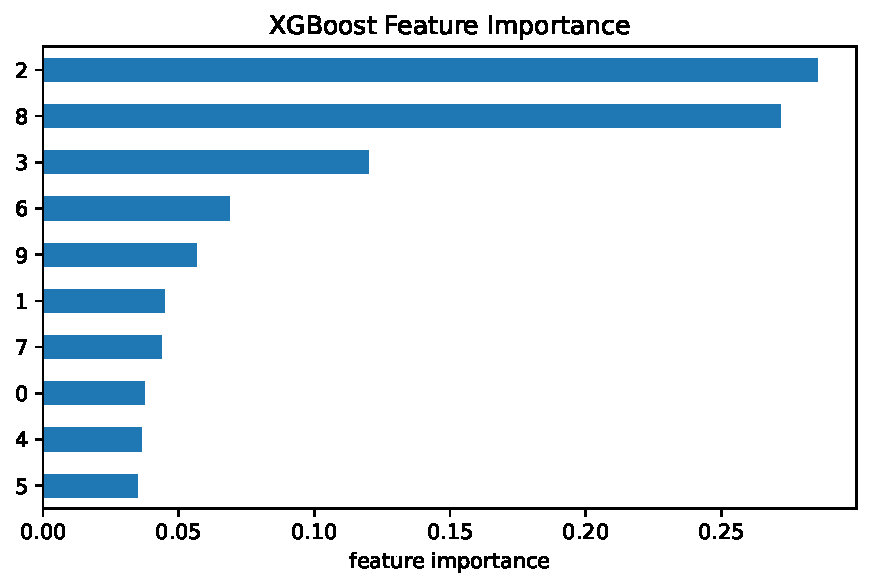
\includegraphics[keepaspectratio]{contents/2/boost_files/figure-pdf/cell-32-output-1.pdf}}

Feature importance describes how much the fitted model uses each
predictor for prediction. It should not be interpreted as a causal
effect.

\part{Unsupervised Learning}

\chapter{Clustering}\label{sec-clustering}

Clustering is an unsupervised learning problem. We observe only a
feature matrix \(X\in\mathbb R^{n\times p}\) and seek to partition the
observations into groups whose members are similar. Unlike
classification, there are no training labels that define the target
categories.

Clustering is commonly used to explore latent subpopulations, summarize
a large dataset with a small number of groups or prototypes, organize
observations for visualization, and generate hypotheses for later
scientific analysis.

\begin{tcolorbox}[enhanced jigsaw, arc=.35mm, bottomrule=.15mm, bottomtitle=1mm, breakable, colback=white, colbacktitle=quarto-callout-caution-color!10!white, colframe=quarto-callout-caution-color-frame, coltitle=black, left=2mm, leftrule=.75mm, opacityback=0, opacitybacktitle=0.6, rightrule=.15mm, title=\textcolor{quarto-callout-caution-color}{\faFire}\hspace{0.5em}{A cluster is not automatically a real category}, titlerule=0mm, toprule=.15mm, toptitle=1mm]

A clustering algorithm produces cluster assignments according to its
objective and tuning choices. The result may reflect meaningful
structure, but it may also reflect feature scaling, outliers, an
unsuitable dissimilarity measure, or a forced choice of the number of
clusters. Interpretation is part of the analysis.

\end{tcolorbox}

Clustering methods differ in their definition of a group. In the notes
we focuses on three major direct clustering paradigms, represented by
one typical method from each:

{\def\LTcaptype{none} % do not increment counter
\begin{longtable}[]{@{}
  >{\raggedright\arraybackslash}p{(\linewidth - 4\tabcolsep) * \real{0.3333}}
  >{\raggedright\arraybackslash}p{(\linewidth - 4\tabcolsep) * \real{0.3333}}
  >{\raggedright\arraybackslash}p{(\linewidth - 4\tabcolsep) * \real{0.3333}}@{}}
\toprule\noalign{}
\begin{minipage}[b]{\linewidth}\raggedright
Family
\end{minipage} & \begin{minipage}[b]{\linewidth}\raggedright
Typical method
\end{minipage} & \begin{minipage}[b]{\linewidth}\raggedright
What defines a cluster?
\end{minipage} \\
\midrule\noalign{}
\endhead
\bottomrule\noalign{}
\endlastfoot
Centroid-based & K-means & observations close to the same center \\
Hierarchical & agglomerative hierarchical clustering & observations
joined through a sequence of merges \\
Density-based & DBSCAN & observations connected through dense regions \\
\end{longtable}
}

Many other clustering approaches exist, including graph-based and
representation-based methods. The three paradigms here are emphasized
because they give distinct direct definitions of what constitutes a
cluster. We use one representative algorithm from each paradigm to
illustrate the main ideas.

\begin{tcolorbox}[enhanced jigsaw, arc=.35mm, bottomrule=.15mm, bottomtitle=1mm, breakable, colback=white, colbacktitle=quarto-callout-note-color!10!white, colframe=quarto-callout-note-color-frame, coltitle=black, left=2mm, leftrule=.75mm, opacityback=0, opacitybacktitle=0.6, rightrule=.15mm, title=\textcolor{quarto-callout-note-color}{\faInfo}\hspace{0.5em}{Distance, Similarity, and Scaling}, titlerule=0mm, toprule=.15mm, toptitle=1mm]

Most clustering methods require a notion of similarity or dissimilarity.
For numerical data, a common choice is Euclidean distance:
\(d(x_i,x_j)=\norm{x_i-x_j}_2=\sqrt{\sum_{\ell=1}^p(x_{i\ell}-x_{j\ell})^2}\).

The distance defines what the algorithm means by \emph{similar}.
Changing the features, their scales, or the dissimilarity measure
changes the clustering problem. Features with larger numerical ranges
can dominate distance calculations, so standardization is often useful
when feature scales are not directly comparable.

Euclidean distance is not the only option. Manhattan distance, cosine
similarity, or a domain-specific measure may be more appropriate
depending on the structure one hopes to discover.

\end{tcolorbox}

\begin{tcolorbox}[enhanced jigsaw, arc=.35mm, bottomrule=.15mm, bottomtitle=1mm, breakable, colback=white, colbacktitle=quarto-callout-note-color!10!white, colframe=quarto-callout-note-color-frame, coltitle=black, left=2mm, leftrule=.75mm, opacityback=0, opacitybacktitle=0.6, rightrule=.15mm, title=\textcolor{quarto-callout-note-color}{\faInfo}\hspace{0.5em}{Scaling is a modeling decision}, titlerule=0mm, toprule=.15mm, toptitle=1mm]

Standardize when numerical scales are arbitrary or incomparable. Do not
standardize automatically when the original magnitudes are
scientifically meaningful, such as comparable pixel intensities or
measurements already expressed on a common scale.

\end{tcolorbox}

\section{Evaluating a Clustering}\label{evaluating-a-clustering}

Evaluating clustering differs from evaluating supervised learning. In
classification or regression, the response variable defines what a
correct prediction means, and performance can be measured on held-out
labeled data. In clustering, group membership is not observed during
fitting. The algorithm produces cluster assignments, but several
different assignments may be reasonable for the same dataset depending
on the features, scaling, distance, and scientific question.

For this reason, clustering evaluation usually separates two questions:

\begin{itemize}
\tightlist
\item
  Are the fitted clusters geometrically coherent in the observed feature
  space?
\item
  If reference labels are available, how well do the cluster assignments
  agree with those external labels?
\end{itemize}

Although some evaluation measures are commonly associated with
particular clustering methods, the focus here is on the metrics
themselves; the corresponding algorithms are discussed in later
sections.

\subsection{WCSS (or Inertia)}\label{wcss-or-inertia}

Internal clustering metrics use only the observations and their cluster
assignments. They can compare values of \(K\), initializations, or
methods, but only when the observations, features, scaling, and distance
are held fixed. They measure geometric properties of the fitted
clustering, not whether the clusters correspond to meaningful external
categories.

Two common internal metrics are WCSS and the silhouette value.

The examples below use a small hypothetical dataset to illustrate the
mechanics of the evaluation. We first visualize one set of cluster
assignments.

\begin{Shaded}
\begin{Highlighting}[]
\ImportTok{import}\NormalTok{ numpy }\ImportTok{as}\NormalTok{ np}
\ImportTok{import}\NormalTok{ matplotlib.pyplot }\ImportTok{as}\NormalTok{ plt}

\NormalTok{X\_eval }\OperatorTok{=}\NormalTok{ np.array([}
\NormalTok{    [}\FloatTok{0.0}\NormalTok{, }\FloatTok{0.1}\NormalTok{],}
\NormalTok{    [}\FloatTok{0.2}\NormalTok{, }\FloatTok{0.0}\NormalTok{],}
\NormalTok{    [}\FloatTok{0.1}\NormalTok{, }\FloatTok{0.3}\NormalTok{],}
\NormalTok{    [}\FloatTok{4.0}\NormalTok{, }\FloatTok{4.1}\NormalTok{],}
\NormalTok{    [}\FloatTok{4.2}\NormalTok{, }\FloatTok{3.9}\NormalTok{],}
\NormalTok{    [}\FloatTok{3.8}\NormalTok{, }\FloatTok{4.0}\NormalTok{],}
\NormalTok{    [}\FloatTok{8.0}\NormalTok{, }\FloatTok{0.0}\NormalTok{],}
\NormalTok{    [}\FloatTok{8.2}\NormalTok{, }\FloatTok{0.2}\NormalTok{],}
\NormalTok{    [}\FloatTok{7.9}\NormalTok{, }\OperatorTok{{-}}\FloatTok{0.1}\NormalTok{],}
\NormalTok{    [}\FloatTok{8.1}\NormalTok{, }\FloatTok{0.1}\NormalTok{],}
\NormalTok{])}

\NormalTok{cluster\_eval }\OperatorTok{=}\NormalTok{ np.array([}\DecValTok{0}\NormalTok{, }\DecValTok{0}\NormalTok{, }\DecValTok{0}\NormalTok{, }\DecValTok{1}\NormalTok{, }\DecValTok{1}\NormalTok{, }\DecValTok{1}\NormalTok{, }\DecValTok{2}\NormalTok{, }\DecValTok{2}\NormalTok{, }\DecValTok{2}\NormalTok{, }\DecValTok{2}\NormalTok{])}

\NormalTok{plt.scatter(X\_eval[:, }\DecValTok{0}\NormalTok{], X\_eval[:, }\DecValTok{1}\NormalTok{], c}\OperatorTok{=}\NormalTok{cluster\_eval)}
\NormalTok{plt.gcf().set\_size\_inches(}\DecValTok{5}\NormalTok{, }\DecValTok{3}\NormalTok{)}
\end{Highlighting}
\end{Shaded}

\pandocbounded{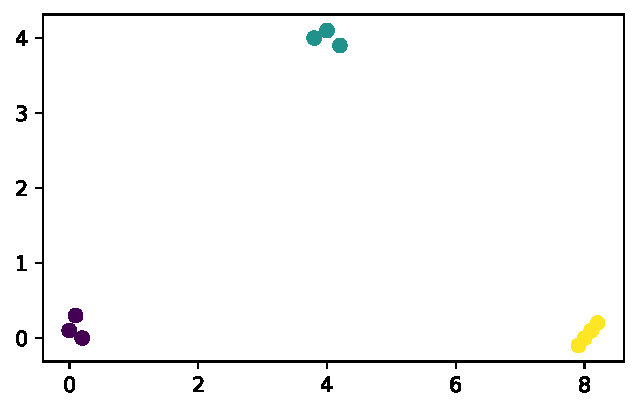
\includegraphics[keepaspectratio]{contents/3/cluster_files/figure-pdf/cell-2-output-1.pdf}}

The within-cluster sum of squares (WCSS) measures the total squared
distance from each observation to the center of its assigned cluster. If
\(\mu_k\) is the center of cluster \(C_k\), then

\[
\operatorname{WCSS}
=
\sum_{k=1}^K
\sum_{i\in C_k}
\norm{x_i-\mu_k}_2^2.
\]

WCSS can be computed once cluster assignments and centers are specified.
For arbitrary cluster labels, a natural choice is to set each center to
the mean of its assigned observations. If only centers are given, as in
the K-means assignment step, each observation is first assigned to its
nearest center and WCSS is then computed from those assignments.

For K-means, WCSS is both the fitting objective and an internal measure
of cluster compactness. It plays a role similar to the residual sum of
squares (RSS) in regression: smaller values indicate that observations
are closer to their fitted centers.

WCSS can be computed for any assignment of observations to clusters
using any methods. However, it is most naturally associated with K-means
because K-means explicitly minimizes WCSS during fitting. For clustering
methods designed to detect non-spherical or density-based structures,
WCSS may not provide a meaningful assessment of clustering quality.

In \texttt{sklearn}, WCSS is also called inertia and is stored as
\texttt{.inertia\_} on a fitted \texttt{KMeans} object. This is the WCSS
for the fitted centers, specifically the best solution among the
initializations tried. There is no general \texttt{sklearn} API for
computing WCSS from arbitrary centers or labels.

\begin{Shaded}
\begin{Highlighting}[]
\ImportTok{from}\NormalTok{ sklearn.cluster }\ImportTok{import}\NormalTok{ KMeans}

\NormalTok{kmeans\_eval }\OperatorTok{=}\NormalTok{ KMeans(n\_clusters}\OperatorTok{=}\DecValTok{3}\NormalTok{, n\_init}\OperatorTok{=}\DecValTok{20}\NormalTok{, random\_state}\OperatorTok{=}\DecValTok{1}\NormalTok{)}
\NormalTok{kmeans\_eval.fit(X\_eval)}
\NormalTok{kmeans\_eval.inertia\_}
\end{Highlighting}
\end{Shaded}

\begin{verbatim}
0.26666666666666655
\end{verbatim}

Click to expand.

For this example, the three fitted groups have centers

\[
\mu_0
=
\frac{(0.0,0.1)+(0.2,0.0)+(0.1,0.3)}{3}
=
\left(0.1,\frac{2}{15}\right),
\]

\[
\mu_1
=
\frac{(4.0,4.1)+(4.2,3.9)+(3.8,4.0)}{3}
=
(4.0,4.0),
\]

\[
\mu_2
=
\frac{(8.0,0.0)+(8.2,0.2)+(7.9,-0.1)+(8.1,0.1)}{4}
=
(8.05,0.05).
\]

Plugging these centers into the WCSS formula gives

\[
\begin{aligned}
\operatorname{WCSS}_0
=&
\left\|(0.0,0.1)-\left(0.1,\frac{2}{15}\right)\right\|^2
+\left\|(0.2,0.0)-\left(0.1,\frac{2}{15}\right)\right\|^2
+\left\|(0.1,0.3)-\left(0.1,\frac{2}{15}\right)\right\|^2\\
=&
\frac{1}{15},\\
\operatorname{WCSS}_1
=&
\|(4.0,4.1)-(4.0,4.0)\|^2
+\|(4.2,3.9)-(4.0,4.0)\|^2
+\|(3.8,4.0)-(4.0,4.0)\|^2\\
=&0.10,\\
\operatorname{WCSS}_2
=&
\|(8.0,0.0)-(8.05,0.05)\|^2
+\|(8.2,0.2)-(8.05,0.05)\|^2+\|(7.9,-0.1)-(8.05,0.05)\|^2
+\|(8.1,0.1)-(8.05,0.05)\|^2\\
=&0.10.
\end{aligned}
\]

Therefore,

\[
\operatorname{WCSS}
=
\frac{1}{15}+0.10+0.10
\approx
0.267.
\]

Smaller inertia means observations are closer to their assigned centers.
However, inertia always decreases as \(K\) increases and becomes zero
when every distinct observation is its own cluster. Therefore, its
absolute minimum cannot be used to choose \(K\).

\subsection{Silhouette Value}\label{silhouette-value}

The {Silhouette} value is another internal evaluation measure. It
evaluates both within-cluster cohesion and separation from nearby
clusters. For observation \(i\), define:

\begin{itemize}
\tightlist
\item
  \(a(i)\) as its average distance to other observations in its own
  cluster;
\item
  \(b(i)\) as the smallest average distance to observations in another
  cluster.
\end{itemize}

The silhouette value is

\[
s(i)
=
\frac{b(i)-a(i)}
{\max\{a(i),b(i)\}}.
\]

It lies between \(-1\) and \(1\):

\begin{itemize}
\tightlist
\item
  values near \(1\) indicate a well-separated observation;
\item
  values near \(0\) indicate an observation near a cluster boundary;
\item
  negative values suggest that another cluster may be closer.
\end{itemize}

The overall silhouette score is the average of \(s(i)\) over all
observations. Larger values are preferred. It requires at least two
nonempty clusters.

\begin{Shaded}
\begin{Highlighting}[]
\ImportTok{from}\NormalTok{ sklearn.metrics }\ImportTok{import}\NormalTok{ silhouette\_score}

\NormalTok{silhouette\_score(X\_eval, cluster\_eval)}
\end{Highlighting}
\end{Shaded}

\begin{verbatim}
0.952562475841761
\end{verbatim}

Click to expand.

For example, consider the first observation \(x_1=(0.0,0.1)\), which
belongs to cluster 0. Its average distance to the other observations in
its own cluster is

\[
a(1)
=
\frac{
\|(0.0,0.1)-(0.2,0.0)\|
+
\|(0.0,0.1)-(0.1,0.3)\|
}{2}
\approx
0.224.
\]

Next compute its average distance to each other cluster:

\[
\begin{aligned}
d(1,C_1)
&=
\frac{
\|(0.0,0.1)-(4.0,4.1)\|
+\|(0.0,0.1)-(4.2,3.9)\|
+\|(0.0,0.1)-(3.8,4.0)\|
}{3}\\
&\approx 5.589,
\end{aligned}
\]

and

\[
\begin{aligned}
d(1,C_2)
&=
\frac{
\|(0.0,0.1)-(8.0,0.0)\|
+\|(0.0,0.1)-(8.2,0.2)\|
+\|(0.0,0.1)-(7.9,-0.1)\|
+\|(0.0,0.1)-(8.1,0.1)\|
}{4}\\
&\approx 8.051.
\end{aligned}
\]

Therefore,

\[
b(1)=\min\{5.589,8.051\}=5.589,
\]

and the silhouette value for this observation is

\[
s(1)
=
\frac{b(1)-a(1)}{\max\{a(1),b(1)\}}
=
\frac{5.589-0.224}{5.589}
\approx
0.960.
\]

The Silhouette score for the whole dataset is the mean of the score for
each individual observation.

This score is close to 1, indicating that most observations are much
closer to observations in their assigned cluster than to observations in
other clusters.

\subsection{Stability}\label{stability}

A useful clustering should not change drastically under small,
reasonable changes to the analysis. Stability asks whether the same
broad grouping appears when the data or fitting procedure is slightly
perturbed.

Common checks include rerunning the method with different random seeds,
changing tuning parameters slightly, refitting after small changes to
preprocessing, or clustering bootstrap or subsampled versions of the
data. The numeric cluster labels themselves do not need to match,
because labels are arbitrary. What matters is whether similar
observations remain grouped together.

Stability is not the same as correctness. A clustering can be stable
because a method has a strong geometric bias, even if the resulting
groups are not scientifically meaningful. It should therefore be
considered together with internal scores, visual inspection when
possible, and interpretation in the original features.

\subsection{Interpretation in the Original
Features}\label{interpretation-in-the-original-features}

Numerical scores do not explain what a cluster represents. After fitting
a clustering, the groups should be described using the original
variables. For tabular data, a simple interpretation step is to
summarize each feature by cluster.

\begin{Shaded}
\begin{Highlighting}[]
\ImportTok{import}\NormalTok{ pandas }\ImportTok{as}\NormalTok{ pd}

\NormalTok{cluster\_summary }\OperatorTok{=}\NormalTok{ (}
\NormalTok{    pd.DataFrame(X\_eval, columns}\OperatorTok{=}\NormalTok{[}\StringTok{"x1"}\NormalTok{, }\StringTok{"x2"}\NormalTok{])}
\NormalTok{    .assign(cluster}\OperatorTok{=}\NormalTok{cluster\_eval)}
\NormalTok{    .groupby(}\StringTok{"cluster"}\NormalTok{)}
\NormalTok{    .agg([}\StringTok{"mean"}\NormalTok{, }\StringTok{"std"}\NormalTok{, }\StringTok{"size"}\NormalTok{])}
\NormalTok{)}

\NormalTok{cluster\_summary}
\end{Highlighting}
\end{Shaded}

{\def\LTcaptype{none} % do not increment counter
\begin{longtable}[]{@{}lllllll@{}}
\toprule\noalign{}
& \multicolumn{3}{l}{%
x1} & \multicolumn{3}{l@{}}{%
x2} \\
& mean & std & size & mean & std & size \\
cluster & & & & & & \\
\midrule\noalign{}
\endhead
\bottomrule\noalign{}
\endlastfoot
0 & 0.10 & 0.100000 & 3 & 0.133333 & 0.152753 & 3 \\
1 & 4.00 & 0.200000 & 3 & 4.000000 & 0.100000 & 3 \\
2 & 8.05 & 0.129099 & 4 & 0.050000 & 0.129099 & 4 \\
\end{longtable}
}

\begin{tcolorbox}[enhanced jigsaw, arc=.35mm, bottomrule=.15mm, bottomtitle=1mm, breakable, colback=white, colbacktitle=quarto-callout-caution-color!10!white, colframe=quarto-callout-caution-color-frame, coltitle=black, left=2mm, leftrule=.75mm, opacityback=0, opacitybacktitle=0.6, rightrule=.15mm, title=\textcolor{quarto-callout-caution-color}{\faFire}\hspace{0.5em}{No single score validates a clustering}, titlerule=0mm, toprule=.15mm, toptitle=1mm]

Internal metrics and Rand-index-based agreement measures answer
different questions. A useful clustering should be geometrically
coherent, reasonably stable, and interpretable for the problem at hand.

\end{tcolorbox}

\subsection{Optional: Rand Index}\label{optional-rand-index}

Click to expand.

When reference labels are available, they can be used after clustering
for external validation. This setting is common in simulations,
benchmark datasets, or applications where external categories are known
but intentionally withheld from the clustering algorithm.

External validation does not turn clustering into supervised learning
because the reference labels are not used during fitting. Instead, it
asks how well the cluster assignments agree with an external reference
labeling.

The Rand index compares cluster assignments with reference labels by
considering all pairs of observations. A pair is counted as an agreement
if the two observations are assigned to the same cluster and have the
same reference label, or if they are assigned to different clusters and
have different reference labels. The index lies between \(0\) and \(1\),
with larger values indicating stronger agreement.

Let \(a\) be the number of observation pairs that are grouped together
by both labelings. That is, the two observations have the same cluster
assignment and also have the same reference label. Let \(b\) be the
number of observation pairs that are separated by both labelings. That
is, the two observations have different cluster assignments and also
have different reference labels. Since there are \({n \choose 2}\) total
pairs, the Rand index is

\[
\operatorname{RI}
=
\frac{a+b}{{n \choose 2}}.
\]

\begin{Shaded}
\begin{Highlighting}[]
\ImportTok{from}\NormalTok{ sklearn.metrics }\ImportTok{import}\NormalTok{ rand\_score}

\NormalTok{reference\_labels }\OperatorTok{=}\NormalTok{ np.array([}\DecValTok{1}\NormalTok{, }\DecValTok{1}\NormalTok{, }\DecValTok{1}\NormalTok{, }\DecValTok{2}\NormalTok{, }\DecValTok{2}\NormalTok{, }\DecValTok{2}\NormalTok{, }\DecValTok{2}\NormalTok{, }\DecValTok{3}\NormalTok{, }\DecValTok{3}\NormalTok{, }\DecValTok{3}\NormalTok{])}
\NormalTok{cluster\_assignments }\OperatorTok{=}\NormalTok{ np.array([}\DecValTok{0}\NormalTok{, }\DecValTok{0}\NormalTok{, }\DecValTok{0}\NormalTok{, }\DecValTok{1}\NormalTok{, }\DecValTok{1}\NormalTok{, }\DecValTok{2}\NormalTok{, }\DecValTok{2}\NormalTok{, }\DecValTok{2}\NormalTok{, }\DecValTok{2}\NormalTok{, }\DecValTok{2}\NormalTok{])}

\NormalTok{rand\_score(reference\_labels, cluster\_assignments)}
\end{Highlighting}
\end{Shaded}

\begin{verbatim}
0.7777777777777778
\end{verbatim}

The diagram below shows where the two labelings agree and disagree. The
reference labels define groups \(\{1,2,3\}\), while the clustering
algorithm returns cluster labels \(\{0,1,2\}\). The mismatch occurs
because reference class 2 is split across clusters 1 and 2, and cluster
2 also contains observations from reference class 3.

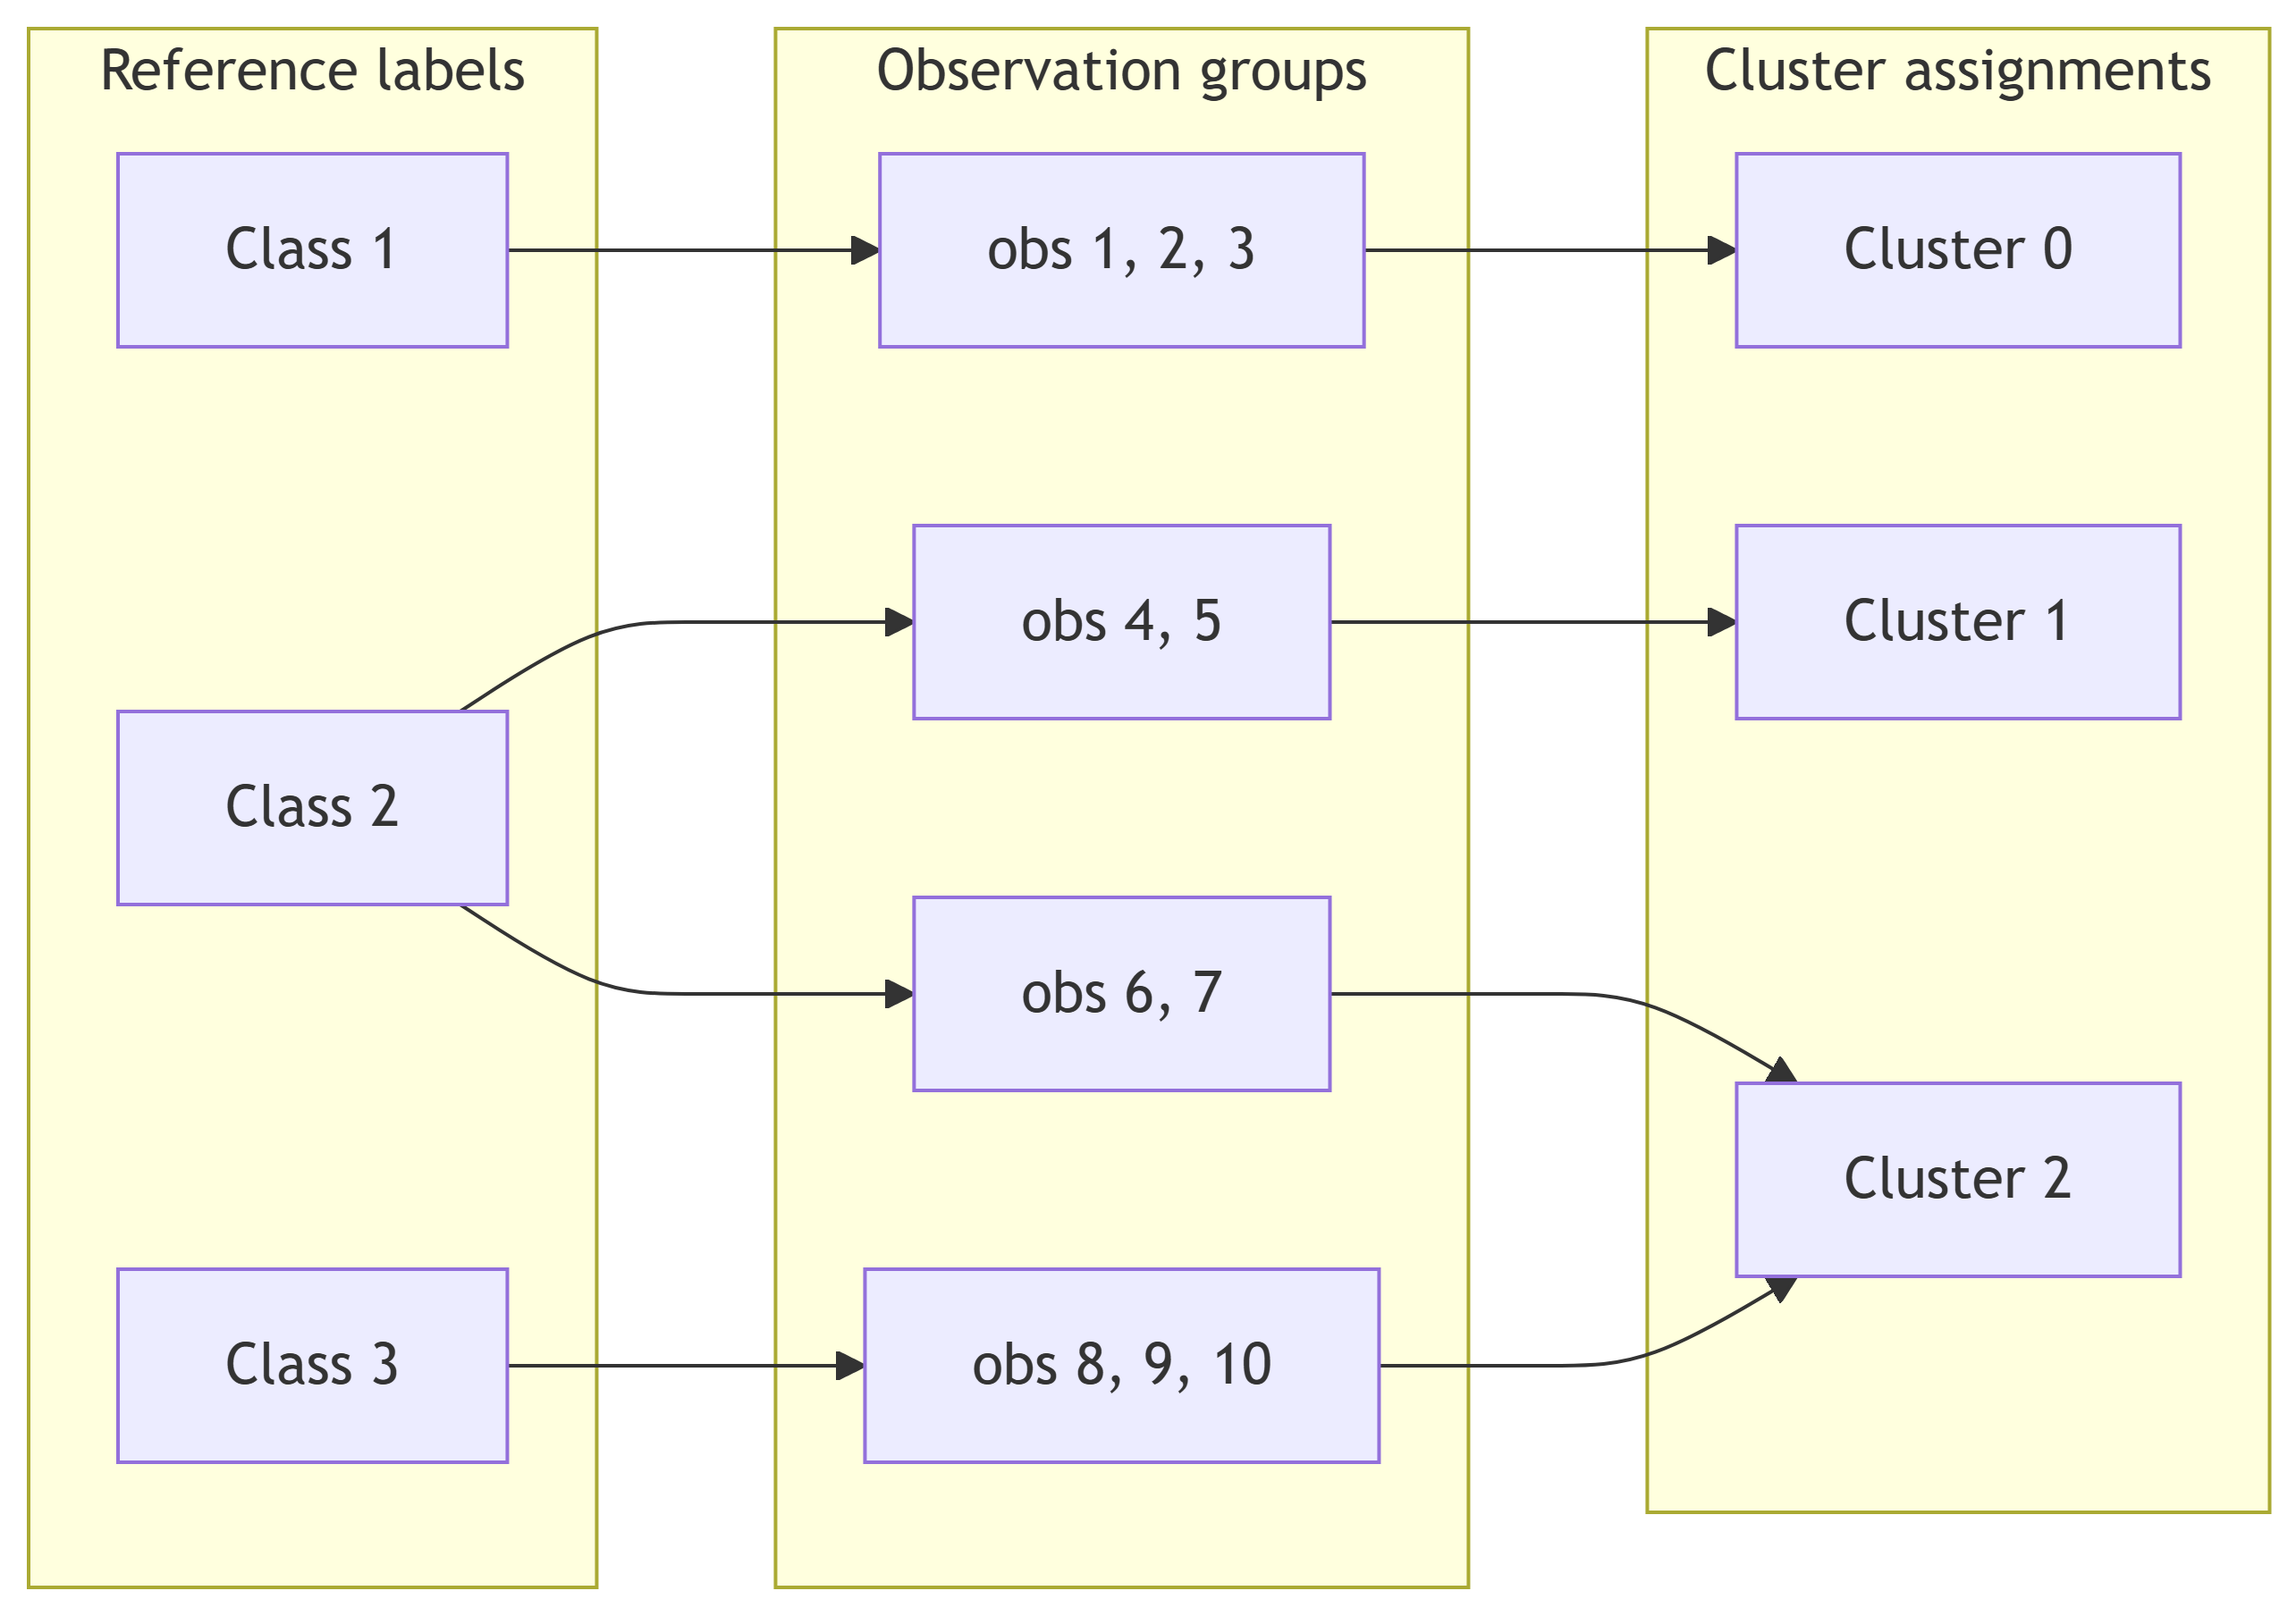
\includegraphics[width=6.69in,height=4.71in]{contents/3/cluster_files/figure-latex/mermaid-figure-1.png}

The diagram also gives a quick way to compute the four pair counts:

\begin{itemize}
\tightlist
\item
  \(a\): pairs together in both labelings. Add \({m\choose 2}\) within
  each middle observation group:
  \(a={3\choose 2}+{2\choose 2}+{2\choose 2}+{3\choose 2}=8\).
\item
  \(c\): pairs together in the reference labels but separated by the
  cluster assignments. Reference class 2 is split into groups of sizes 2
  and 2, so \(c=2\times 2=4\).
\item
  \(d\): pairs separated by the reference labels but together in the
  cluster assignments. Cluster 2 contains 2 observations from reference
  class 2 and 3 observations from reference class 3, so
  \(d=2\times 3=6\).
\item
  \(b\): pairs separated by both labelings. The fastest calculation is
  subtraction from all pairs:
\end{itemize}

\[
b
=
{10\choose 2}-a-c-d
=
45-8-4-6
=
27.
\]

There are \({10 \choose 2}=45\) observation pairs. Among them, \(a=8\)
pairs are grouped together by both labelings, and \(b=27\) pairs are
separated by both labelings. Therefore,

\[
\operatorname{RI}
=
\frac{8+27}{45}
\approx
0.778.
\]

\subsection{Optional: Adjusted Rand
Index}\label{optional-adjusted-rand-index}

Click to expand.

The Rand index can be high even when two labelings agree partly by
chance, especially when there are many pairs of observations. The
adjusted Rand index corrects for this chance agreement.

\begin{example}[A relatively high Rand index can be
misleading]\protect\hypertarget{exm-high-rand-score}{}\label{exm-high-rand-score}

Suppose the reference labels contain two groups of equal size, but the
clustering algorithm assigns every observation to its own cluster:

{\def\LTcaptype{none} % do not increment counter
\begin{longtable}[]{@{}lllllllllll@{}}
\toprule\noalign{}
Reference label & 1 & 1 & 1 & 1 & 1 & 2 & 2 & 2 & 2 & 2 \\
\midrule\noalign{}
\endhead
\bottomrule\noalign{}
\endlastfoot
Cluster assignment & 0 & 1 & 2 & 3 & 4 & 5 & 6 & 7 & 8 & 9 \\
\end{longtable}
}

This clustering does not recover the two reference groups. However, the
Rand index is still above \(0.5\) because many pairs from different
reference classes are also placed in different clusters. In this
example, \(a=0\) and \(b=25\), so

\[
\operatorname{RI}
=
\frac{0+25}{{10\choose 2}}
=
\frac{25}{45}
\approx
0.556.
\]

\begin{Shaded}
\begin{Highlighting}[]
\ImportTok{from}\NormalTok{ sklearn.metrics }\ImportTok{import}\NormalTok{ rand\_score}

\NormalTok{reference\_labels }\OperatorTok{=}\NormalTok{ [}\DecValTok{1}\NormalTok{, }\DecValTok{1}\NormalTok{, }\DecValTok{1}\NormalTok{, }\DecValTok{1}\NormalTok{, }\DecValTok{1}\NormalTok{, }\DecValTok{2}\NormalTok{, }\DecValTok{2}\NormalTok{, }\DecValTok{2}\NormalTok{, }\DecValTok{2}\NormalTok{, }\DecValTok{2}\NormalTok{]}
\NormalTok{cluster\_assignments }\OperatorTok{=}\NormalTok{ [}\DecValTok{0}\NormalTok{, }\DecValTok{1}\NormalTok{, }\DecValTok{2}\NormalTok{, }\DecValTok{3}\NormalTok{, }\DecValTok{4}\NormalTok{, }\DecValTok{5}\NormalTok{, }\DecValTok{6}\NormalTok{, }\DecValTok{7}\NormalTok{, }\DecValTok{8}\NormalTok{, }\DecValTok{9}\NormalTok{]}

\NormalTok{rand\_score(reference\_labels, cluster\_assignments)}
\end{Highlighting}
\end{Shaded}

\begin{verbatim}
0.5555555555555556
\end{verbatim}

\end{example}

The adjusted Rand index compares the observed pairwise agreement with
the agreement expected from random labelings with similar group sizes.
Suppose \(n_{ij}\) is the number of observations that are in reference
class \(i\) and cluster \(j\). Let

\[
a_i=\sum_j n_{ij},
\qquad
b_j=\sum_i n_{ij}.
\]

Thus, \(a_i\) is the size of reference class \(i\), and \(b_j\) is the
size of cluster \(j\). Then the adjusted Rand index is

\[
\operatorname{ARI}
=
\frac{
\sum_{ij}{n_{ij}\choose 2}
-
\frac{
\sum_i {a_i\choose 2}\sum_j {b_j\choose 2}
}{{n\choose 2}}
}{
\frac{1}{2}
\left[
\sum_i {a_i\choose 2}
+
\sum_j {b_j\choose 2}
\right]
-
\frac{
\sum_i {a_i\choose 2}\sum_j {b_j\choose 2}
}{{n\choose 2}}
}.
\]

The formula has three main parts:

\begin{itemize}
\tightlist
\item
  \(\sum_{ij}{n_{ij}\choose 2}\) is the observed number of pairs that
  are placed together in both the reference labels and the cluster
  assignments.
\item
  \(\frac{\sum_i {a_i\choose 2}\sum_j {b_j\choose 2}}{{n\choose 2}}\) is
  the expected number of such agreeing pairs under random labelings with
  the same class sizes and cluster sizes.
\item
  \(\frac{1}{2}\left[\sum_i {a_i\choose 2}+\sum_j {b_j\choose 2}\right]\)
  is the average of the largest pair counts implied by the two marginal
  labelings.
\end{itemize}

Conceptually, the adjusted Rand index has the form

\[
\operatorname{ARI}
=
\frac{
\text{observed pairwise agreement}
-
\text{expected pairwise agreement}
}{
\text{maximum pairwise agreement}
-
\text{expected pairwise agreement}
}.
\]

The key difference between the Rand index and the adjusted Rand index is
that the Rand index measures raw pairwise agreement, while the adjusted
Rand index measures pairwise agreement after correcting for chance. This
correction matters because many pairs may agree simply because they are
separated in both labelings, even when the clustering does not recover
the reference groups.

Click to expand.

Let \(N\) be the total number of paris. The Rand index is

\[
\operatorname{RI}=\frac{a+b}{N}.
\]

Recall that

\begin{itemize}
\tightlist
\item
  \(a\) is the number of pairs together in both labelings
\item
  \(b\) is the number of pairs separated by both labelings
\item
  \(c\) is the number of pairs together in the reference labels but
  separated by the cluster assignments
\item
  \(d\) is the number of pairs separated by the reference labels but
  together in the cluster assignments
\end{itemize}

Then

\begin{itemize}
\tightlist
\item
  The total number of pairs placed together in the reference labeling is
  \(R=a+c\).
\item
  The total number of pairs placed together in the cluster assignment is
  \(C=a+d\).
\end{itemize}

Therefore, \(c=R-a\), and \(d=C-a\). Because \(a+b+c+d=N\),

\[
\begin{split}
b
&=N-a-c-d\\
&=N-a-(R-a)-(C-a)\\
&=N-R-C+a.
\end{split}
\]

Hence, the observed number of agreeing pairs can be written as

\[
\begin{split}
a+b
&=a+(N-R-C+a)\\
&=N-R-C+2a.
\end{split}
\]

Now we update RI to be ARI by removing expected assignments: \[
\operatorname{ARI}
=
\frac{
\text{observed pairwise agreement}
-
\text{expected pairwise agreement}
}{
\text{maximum pairwise agreement}
-
\text{expected pairwise agreement}
}=\frac{a+b-\Exp[a+b]}{N-\Exp[a+b]}.
\]

There are \(R\) pairs placed together in the reference labeling, and
each such pair has probability \(C/N\) of also being placed together in
the cluster assignment. Therefore under random labeling with the same
reference-class sizes and cluster sizes, the expected number of pairs
placed together in both labelings is

\[
\Exp[a]=\frac{RC}{N}.
\]

Similarly, the expected number of pairs separated in both labelings is

\[
\Exp[b]=\frac{(N-R)(N-C)}{N}.
\]

Therefore, the expected total pairwise agreement is

\[
\begin{split}
\Exp[a+b]
&=\frac{RC}{N}+\frac{(N-R)(N-C)}{N}\\
&=N-R-C+2\frac{RC}{N}.
\end{split}
\]

Then

\[
\operatorname{ARI}
=\frac{a+b-\Exp[a+b]}{N-\Exp[a+b]}.
\]

The numerator is

\[
\begin{split}
(a+b)-E[a+b]
&=(N-R-C+2a)
-\left(N-R-C+2\frac{RC}{N}\right)\\
&=2\left(a-\frac{RC}{N}\right).
\end{split}
\]

The denominator is

\[
\begin{split}
N-E[a+b]
&=N-\left(N-R-C+2\frac{RC}{N}\right)\\
&=R+C-2\frac{RC}{N}\\
&=2\left(\frac{R+C}{2}-\frac{RC}{N}\right).
\end{split}
\]

Therefore

\[
\operatorname{ARI}
=\frac{a-\dfrac{RC}{N}}
{\dfrac{1}{2}(R+C)-\dfrac{RC}{N}}.
\]

Finally, substituting

\[
a=\sum_{i,j}\binom{n_{ij}}{2},
\qquad
R=\sum_i\binom{a_i}{2},
\qquad
C=\sum_j\binom{b_j}{2},
\qquad
N=\binom{n}{2}.
\]

we obtain

\[
\operatorname{ARI}
=
\frac{
\sum_{i,j}\binom{n_{ij}}{2}
-
\frac{
\left(\sum_i\binom{a_i}{2}\right)
\left(\sum_j\binom{b_j}{2}\right)
}{
\binom{n}{2}
}
}{
\frac{1}{2}
\left[
\sum_i\binom{a_i}{2}
+
\sum_j\binom{b_j}{2}
\right]
-
\frac{
\left(\sum_i\binom{a_i}{2}\right)
\left(\sum_j\binom{b_j}{2}\right)
}{
\binom{n}{2}
}
}.
\]

Its interpretation is:

\begin{itemize}
\tightlist
\item
  \(1\) means the two labelings are identical, up to relabeling of the
  clusters;
\item
  values near \(0\) mean the agreement is about what would be expected
  by chance;
\item
  negative values are possible when the agreement is worse than expected
  by chance.
\end{itemize}

This correction is useful because cluster labels themselves are
arbitrary. For example, cluster assignments \texttt{{[}0,\ 0,\ 1,\ 1{]}}
and \texttt{{[}2,\ 2,\ 5,\ 5{]}} describe the same grouping even though
the numeric labels are different.

\begin{example}[A relatively high Rand index can be misleading
(cont.)]\protect\hypertarget{exm-}{}\label{exm-}

Continue from the Example~\ref{exm-high-rand-score}.

\begin{Shaded}
\begin{Highlighting}[]
\ImportTok{from}\NormalTok{ sklearn.metrics }\ImportTok{import}\NormalTok{ adjusted\_rand\_score}

\NormalTok{reference\_labels }\OperatorTok{=}\NormalTok{ [}\DecValTok{1}\NormalTok{, }\DecValTok{1}\NormalTok{, }\DecValTok{1}\NormalTok{, }\DecValTok{1}\NormalTok{, }\DecValTok{1}\NormalTok{, }\DecValTok{2}\NormalTok{, }\DecValTok{2}\NormalTok{, }\DecValTok{2}\NormalTok{, }\DecValTok{2}\NormalTok{, }\DecValTok{2}\NormalTok{]}
\NormalTok{cluster\_assignments }\OperatorTok{=}\NormalTok{ [}\DecValTok{0}\NormalTok{, }\DecValTok{1}\NormalTok{, }\DecValTok{2}\NormalTok{, }\DecValTok{3}\NormalTok{, }\DecValTok{4}\NormalTok{, }\DecValTok{5}\NormalTok{, }\DecValTok{6}\NormalTok{, }\DecValTok{7}\NormalTok{, }\DecValTok{8}\NormalTok{, }\DecValTok{9}\NormalTok{]}

\NormalTok{adjusted\_rand\_score(reference\_labels, cluster\_assignments)}
\end{Highlighting}
\end{Shaded}

\begin{verbatim}
0.0
\end{verbatim}

The adjusted Rand index is \(0\), correctly indicating that the observed
agreement is no greater than what would be expected by chance.

\end{example}

The same score can compare two clustering runs on the same observations.
This is useful for assessing whether the fitted clustering is stable
under small changes in preprocessing, initialization, or resampling.

\begin{Shaded}
\begin{Highlighting}[]
\NormalTok{cluster\_run\_1 }\OperatorTok{=}\NormalTok{ np.array([}\DecValTok{0}\NormalTok{, }\DecValTok{0}\NormalTok{, }\DecValTok{0}\NormalTok{, }\DecValTok{1}\NormalTok{, }\DecValTok{1}\NormalTok{, }\DecValTok{1}\NormalTok{, }\DecValTok{2}\NormalTok{, }\DecValTok{2}\NormalTok{, }\DecValTok{2}\NormalTok{, }\DecValTok{2}\NormalTok{])}
\NormalTok{cluster\_run\_2 }\OperatorTok{=}\NormalTok{ np.array([}\DecValTok{1}\NormalTok{, }\DecValTok{1}\NormalTok{, }\DecValTok{1}\NormalTok{, }\DecValTok{0}\NormalTok{, }\DecValTok{0}\NormalTok{, }\DecValTok{0}\NormalTok{, }\DecValTok{2}\NormalTok{, }\DecValTok{2}\NormalTok{, }\DecValTok{2}\NormalTok{, }\DecValTok{2}\NormalTok{])}

\NormalTok{adjusted\_rand\_score(cluster\_run\_1, cluster\_run\_2)}
\end{Highlighting}
\end{Shaded}

\begin{verbatim}
1.0
\end{verbatim}

This example gives high agreement even though the numeric cluster labels
have changed. That is appropriate because the labels identify groups
only up to relabeling.

\section{Centroid-Based: K-Means
Clustering}\label{centroid-based-k-means-clustering}

K-means represents each cluster by its center. Let \(C_1,\ldots,C_K\) be
a partition of the observations, and let

\[
\mu_k
=
\frac{1}{|C_k|}
\sum_{i\in C_k}x_i
\]

be the center of cluster \(k\).

\begin{definition}[K-means
objective]\protect\hypertarget{def-kmeans}{}\label{def-kmeans}

K-means chooses the partition that minimizes the within-cluster sum of
squares (WCSS):

\[
\operatorname{WCSS}
=
\sum_{k=1}^K
\sum_{i\in C_k}
\norm{x_i-\mu_k}_2^2.
\]

In \texttt{sklearn}, this objective is also called \textbf{inertia}.

\end{definition}

The standard algorithm alternates between two steps:

\begin{enumerate}
\def\labelenumi{\arabic{enumi}.}
\tightlist
\item
  assign each observation to its nearest center;
\item
  replace each center by the mean of its assigned observations.
\end{enumerate}

Each step decreases, or leaves unchanged, the K-means objective. The
algorithm eventually reaches a local optimum, but not necessarily the
global optimum. For this reason, software usually tries several random
initializations.

\subsection{K-means in Python}\label{k-means-in-python}

We use a simulated dataset to illustrate K-means in Python.

We use \texttt{make\_blobs} from \texttt{sklearn.datasets} to generate
500 observations from three latent groups. The data have two features so
that the result can be visualized directly. The colors below show the
generating labels. They are not used when fitting K-means.

\begin{Shaded}
\begin{Highlighting}[]
\ImportTok{import}\NormalTok{ numpy }\ImportTok{as}\NormalTok{ np}
\ImportTok{from}\NormalTok{ sklearn.datasets }\ImportTok{import}\NormalTok{ make\_blobs}
\ImportTok{import}\NormalTok{ matplotlib.pyplot }\ImportTok{as}\NormalTok{ plt}

\NormalTok{X, true\_group }\OperatorTok{=}\NormalTok{ make\_blobs(}
\NormalTok{    n\_samples}\OperatorTok{=}\DecValTok{500}\NormalTok{,}
\NormalTok{    n\_features}\OperatorTok{=}\DecValTok{2}\NormalTok{,}
\NormalTok{    centers}\OperatorTok{=}\DecValTok{3}\NormalTok{,}
\NormalTok{    cluster\_std}\OperatorTok{=}\NormalTok{[}\FloatTok{0.7}\NormalTok{, }\FloatTok{0.9}\NormalTok{, }\FloatTok{0.8}\NormalTok{],}
\NormalTok{    random\_state}\OperatorTok{=}\DecValTok{3}\NormalTok{,}
\NormalTok{)}

\NormalTok{plt.scatter(X[:, }\DecValTok{0}\NormalTok{], X[:, }\DecValTok{1}\NormalTok{], c}\OperatorTok{=}\NormalTok{true\_group)}
\NormalTok{plt.xlabel(}\StringTok{"x1"}\NormalTok{)}
\NormalTok{plt.ylabel(}\StringTok{"x2"}\NormalTok{)}
\NormalTok{plt.title(}\StringTok{"Simulated Groups"}\NormalTok{)}\OperatorTok{;}
\end{Highlighting}
\end{Shaded}

\pandocbounded{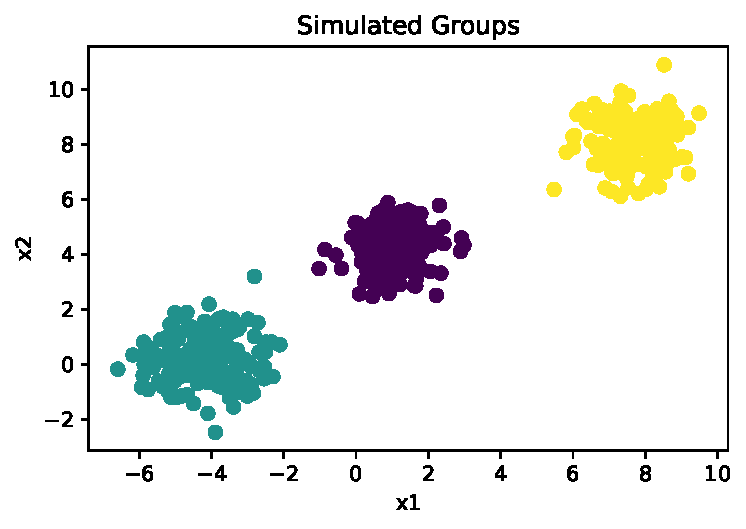
\includegraphics[keepaspectratio]{contents/3/cluster_files/figure-pdf/cell-10-output-1.pdf}}

\texttt{KMeans} follows the usual \texttt{sklearn} interface. Since
clustering is performed on the observed data themselves, we fit the
model to the feature matrix and obtain cluster assignments for the
observations.

For this first illustration, we set \texttt{n\_clusters=3} so that the
fitted result can be compared visually with the simulated groups. This
does not represent how \(K\) is chosen in practice. In real
applications, the number of clusters is usually unknown and must be
treated as a tuning choice.

As mentioned previously, it is recommended to use multiple random
initializations to reduce sensitivity to a poor starting configuration.
The argument \texttt{n\_init=20} runs K-means from 20 different initial
center configurations and retains the solution with the smallest inertia
among those runs.

\protect\phantomsection\label{annotated-cell-242}%
\begin{Shaded}
\begin{Highlighting}[]
\ImportTok{from}\NormalTok{ sklearn.cluster }\ImportTok{import}\NormalTok{ KMeans}

\NormalTok{kmeans }\OperatorTok{=}\NormalTok{ KMeans(n\_clusters}\OperatorTok{=}\DecValTok{3}\NormalTok{, n\_init}\OperatorTok{=}\DecValTok{20}\NormalTok{, random\_state}\OperatorTok{=}\DecValTok{1}\NormalTok{)}
\NormalTok{kmeans.fit(X)}
\NormalTok{cluster }\OperatorTok{=}\NormalTok{ kmeans.predict(X) }\CommentTok{\# \textless{}1\textgreater{}}
\end{Highlighting}
\end{Shaded}

\begin{description}
\tightlist
\item[5CB6E08D-list-annote-1]
You may also use \texttt{cluster\ =\ kmeans.fit\_predict(X)} to combine
the two commands together.
\end{description}

\texttt{cluster} is an array of cluster assignments, one for each
observation. We can then plot the observations with colors indicating
their assigned clusters.

\begin{Shaded}
\begin{Highlighting}[]
\NormalTok{plt.scatter(X[:, }\DecValTok{0}\NormalTok{], X[:, }\DecValTok{1}\NormalTok{], c}\OperatorTok{=}\NormalTok{cluster)}
\NormalTok{plt.scatter(}
\NormalTok{    kmeans.cluster\_centers\_[:, }\DecValTok{0}\NormalTok{],}
\NormalTok{    kmeans.cluster\_centers\_[:, }\DecValTok{1}\NormalTok{],}
\NormalTok{    marker}\OperatorTok{=}\StringTok{"X"}\NormalTok{,}
\NormalTok{    color}\OperatorTok{=}\StringTok{"black"}\NormalTok{,}
\NormalTok{    label}\OperatorTok{=}\StringTok{"centers"}\NormalTok{,}
\NormalTok{)}
\NormalTok{plt.xlabel(}\StringTok{"x1"}\NormalTok{)}
\NormalTok{plt.ylabel(}\StringTok{"x2"}\NormalTok{)}
\NormalTok{plt.title(}\StringTok{"K{-}Means Clustering"}\NormalTok{)}
\NormalTok{plt.legend()}\OperatorTok{;}
\end{Highlighting}
\end{Shaded}

\pandocbounded{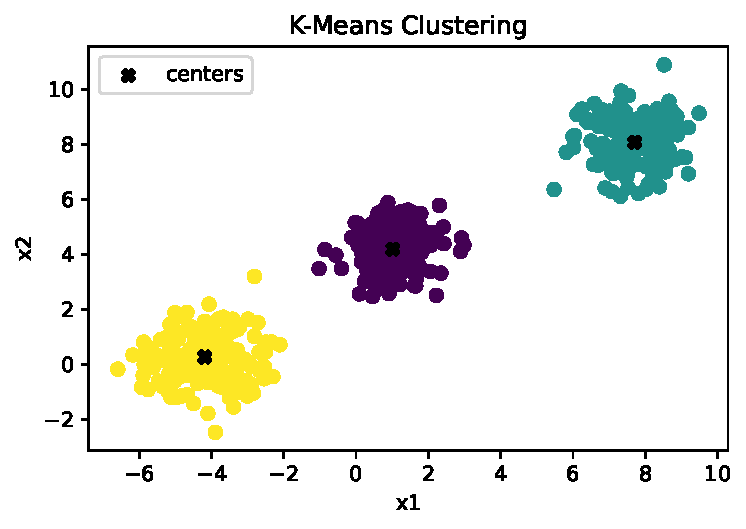
\includegraphics[keepaspectratio]{contents/3/cluster_files/figure-pdf/cell-12-output-1.pdf}}

The fitted centers are available from the model.

\begin{Shaded}
\begin{Highlighting}[]
\NormalTok{kmeans.cluster\_centers\_}
\end{Highlighting}
\end{Shaded}

\begin{verbatim}
array([[ 1.01494239,  4.19111967],
       [ 7.70936555,  8.07424709],
       [-4.1867326 ,  0.2695436 ]])
\end{verbatim}

\begin{tcolorbox}[enhanced jigsaw, arc=.35mm, bottomrule=.15mm, bottomtitle=1mm, breakable, colback=white, colbacktitle=quarto-callout-note-color!10!white, colframe=quarto-callout-note-color-frame, coltitle=black, left=2mm, leftrule=.75mm, opacityback=0, opacitybacktitle=0.6, rightrule=.15mm, title=\textcolor{quarto-callout-note-color}{\faInfo}\hspace{0.5em}{Label switching}, titlerule=0mm, toprule=.15mm, toptitle=1mm]

Cluster labels are arbitrary. A cluster labeled \texttt{0} in one fit
may be labeled \texttt{2} in another fit even when the two clusterings
are equivalent. Interpret the groups through their members and feature
summaries, not the numeric label.

\end{tcolorbox}

\subsection{Tuning Hyperparameters}\label{tuning-hyperparameters-2}

The most important K-means hyperparameter is \texttt{n\_clusters}, the
number of centers to fit. A larger value gives a more detailed
clustering and lowers the within-cluster sum of squares, but it may
split groups that are better interpreted together. A smaller value gives
a coarser summary but may merge distinct groups. There is no universally
correct criterion because the useful level of grouping depends on the
scientific question.

Two common diagnostics for choosing \texttt{n\_clusters} are inertia and
the silhouette score. The elbow plot examines inertia over a range that
includes \(K=1\). The silhouette score compares within-cluster cohesion
with separation from neighboring clusters and is computed only for
\(K\ge 2\).

\begin{Shaded}
\begin{Highlighting}[]
\ImportTok{from}\NormalTok{ sklearn.metrics }\ImportTok{import}\NormalTok{ silhouette\_score}

\NormalTok{inertia\_k }\OperatorTok{=} \BuiltInTok{range}\NormalTok{(}\DecValTok{1}\NormalTok{, }\DecValTok{11}\NormalTok{)}
\NormalTok{inertias }\OperatorTok{=}\NormalTok{ []}
\ControlFlowTok{for}\NormalTok{ k }\KeywordTok{in}\NormalTok{ inertia\_k:}
\NormalTok{    model }\OperatorTok{=}\NormalTok{ KMeans(n\_clusters}\OperatorTok{=}\NormalTok{k, n\_init}\OperatorTok{=}\DecValTok{20}\NormalTok{, random\_state}\OperatorTok{=}\DecValTok{1}\NormalTok{)}
\NormalTok{    model.fit(X)}
\NormalTok{    inertias.append(model.inertia\_)}

\NormalTok{silhouette\_k }\OperatorTok{=} \BuiltInTok{range}\NormalTok{(}\DecValTok{2}\NormalTok{, }\DecValTok{11}\NormalTok{)}
\NormalTok{silhouettes }\OperatorTok{=}\NormalTok{ []}
\ControlFlowTok{for}\NormalTok{ k }\KeywordTok{in}\NormalTok{ silhouette\_k:}
\NormalTok{    model }\OperatorTok{=}\NormalTok{ KMeans(n\_clusters}\OperatorTok{=}\NormalTok{k, n\_init}\OperatorTok{=}\DecValTok{20}\NormalTok{, random\_state}\OperatorTok{=}\DecValTok{1}\NormalTok{)}
\NormalTok{    labels }\OperatorTok{=}\NormalTok{ model.fit\_predict(X)}
\NormalTok{    silhouettes.append(silhouette\_score(X, labels))}
\end{Highlighting}
\end{Shaded}

Plot the two diagnostics together.

\begin{Shaded}
\begin{Highlighting}[]
\ImportTok{import}\NormalTok{ matplotlib.pyplot }\ImportTok{as}\NormalTok{ plt}

\NormalTok{fig, axs }\OperatorTok{=}\NormalTok{ plt.subplots(}\DecValTok{1}\NormalTok{, }\DecValTok{2}\NormalTok{, figsize}\OperatorTok{=}\NormalTok{(}\DecValTok{11}\NormalTok{, }\DecValTok{4}\NormalTok{))}

\NormalTok{axs[}\DecValTok{0}\NormalTok{].plot(inertia\_k, inertias, marker}\OperatorTok{=}\StringTok{"o"}\NormalTok{)}
\NormalTok{axs[}\DecValTok{0}\NormalTok{].set\_xlabel(}\StringTok{"number of clusters K"}\NormalTok{)}
\NormalTok{axs[}\DecValTok{0}\NormalTok{].set\_ylabel(}\StringTok{"inertia"}\NormalTok{)}
\NormalTok{axs[}\DecValTok{0}\NormalTok{].set\_title(}\StringTok{"Elbow Plot"}\NormalTok{)}

\NormalTok{axs[}\DecValTok{1}\NormalTok{].plot(silhouette\_k, silhouettes, marker}\OperatorTok{=}\StringTok{"o"}\NormalTok{)}
\NormalTok{axs[}\DecValTok{1}\NormalTok{].set\_xlabel(}\StringTok{"number of clusters K"}\NormalTok{)}
\NormalTok{axs[}\DecValTok{1}\NormalTok{].set\_ylabel(}\StringTok{"average silhouette"}\NormalTok{)}
\NormalTok{axs[}\DecValTok{1}\NormalTok{].set\_title(}\StringTok{"Silhouette Score"}\NormalTok{)}\OperatorTok{;}
\end{Highlighting}
\end{Shaded}

\pandocbounded{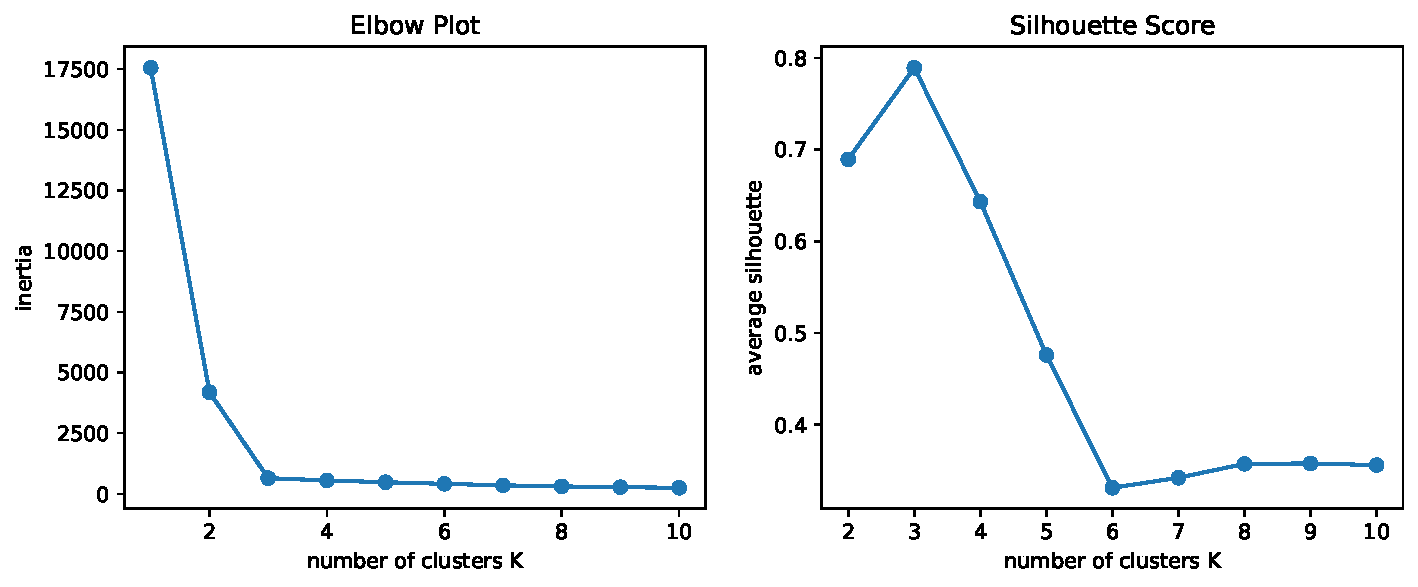
\includegraphics[keepaspectratio]{contents/3/cluster_files/figure-pdf/cell-15-output-1.pdf}}

For inertia, the elbow heuristic looks for the point after which
additional clusters produce only modest improvement. In this example,
the largest improvements occur for small values of \(K\), and \(K=3\) is
a plausible elbow.

For the silhouette score, larger values are preferred. In this example,
the average silhouette score is largest at \(K=3\) over the range
considered.

The two diagnostics can disagree because they measure different aspects
of the cluster assignments. The final choice of \(K\) should be guided
by the analysis goal, stability, and interpretability, not by a single
plot alone. In this simulated example, the diagnostics are consistent
with the illustrative choice \(K=3\).

Other K-means hyperparameters control how the optimization is carried
out:

\begin{itemize}
\tightlist
\item
  \texttt{init} controls how the initial centers are chosen. The default
  \texttt{"k-means++"} spreads initial centers out and is usually
  preferable to purely random initialization.
\item
  \texttt{n\_init} controls how many initial center configurations are
  tried. Since K-means can stop at a local optimum, using several starts
  makes the result less dependent on one unlucky initialization.
\item
  \texttt{max\_iter} is the maximum number of assignment-update steps
  for one initialization.
\item
  \texttt{tol} controls the convergence tolerance. Smaller values ask
  the algorithm to keep iterating until the centers change very little.
\item
  \texttt{random\_state} makes randomized initialization reproducible.
\end{itemize}

For routine analyses, it is common to use \texttt{init="k-means++"}
(which is the default value in the current version of \texttt{sklearn})
and tune \texttt{n\_clusters}, while using a reasonably large
\texttt{n\_init}.

\begin{tcolorbox}[enhanced jigsaw, arc=.35mm, bottomrule=.15mm, bottomtitle=1mm, breakable, colback=white, colbacktitle=quarto-callout-caution-color!10!white, colframe=quarto-callout-caution-color-frame, coltitle=black, left=2mm, leftrule=.75mm, opacityback=0, opacitybacktitle=0.6, rightrule=.15mm, title=\textcolor{quarto-callout-caution-color}{\faFire}\hspace{0.5em}{Diagnostics do not define the scientific answer}, titlerule=0mm, toprule=.15mm, toptitle=1mm]

WCSS and the silhouette score evaluate geometric compactness and
separation under the chosen features, scaling, and distance. They do not
show that the clusters are stable, scientifically meaningful, or useful
for a later decision.

\end{tcolorbox}

\subsection{When K-Means Works Well}\label{when-k-means-works-well}

Because K-means uses squared Euclidean distance to a center, it is most
effective when clusters are:

\begin{itemize}
\tightlist
\item
  compact and approximately spherical;
\item
  separated by their centers;
\item
  reasonably similar in size and spread;
\item
  not dominated by extreme outliers.
\end{itemize}

It can perform poorly on curved clusters, clusters with very different
densities, or data where a mean is not an appropriate prototype.

\begin{Shaded}
\begin{Highlighting}[]
\ImportTok{from}\NormalTok{ sklearn.datasets }\ImportTok{import}\NormalTok{ make\_circles}
\ImportTok{from}\NormalTok{ sklearn.cluster }\ImportTok{import}\NormalTok{ KMeans}
\ImportTok{import}\NormalTok{ matplotlib.pyplot }\ImportTok{as}\NormalTok{ plt}

\NormalTok{X\_circle, true\_circle\_group }\OperatorTok{=}\NormalTok{ make\_circles(}
\NormalTok{    n\_samples}\OperatorTok{=}\DecValTok{500}\NormalTok{, factor}\OperatorTok{=}\FloatTok{0.45}\NormalTok{, noise}\OperatorTok{=}\FloatTok{0.05}\NormalTok{, random\_state}\OperatorTok{=}\DecValTok{1}
\NormalTok{)}

\NormalTok{circle\_kmeans }\OperatorTok{=}\NormalTok{ KMeans(n\_clusters}\OperatorTok{=}\DecValTok{2}\NormalTok{, n\_init}\OperatorTok{=}\DecValTok{20}\NormalTok{, random\_state}\OperatorTok{=}\DecValTok{1}\NormalTok{)}
\NormalTok{circle\_cluster }\OperatorTok{=}\NormalTok{ circle\_kmeans.fit\_predict(X\_circle)}

\NormalTok{fig, axs }\OperatorTok{=}\NormalTok{ plt.subplots(}\DecValTok{1}\NormalTok{, }\DecValTok{2}\NormalTok{, figsize}\OperatorTok{=}\NormalTok{(}\DecValTok{10}\NormalTok{, }\DecValTok{4}\NormalTok{), sharex}\OperatorTok{=}\VariableTok{True}\NormalTok{, sharey}\OperatorTok{=}\VariableTok{True}\NormalTok{)}

\NormalTok{axs[}\DecValTok{0}\NormalTok{].scatter(X\_circle[:, }\DecValTok{0}\NormalTok{], X\_circle[:, }\DecValTok{1}\NormalTok{], c}\OperatorTok{=}\NormalTok{true\_circle\_group)}
\NormalTok{axs[}\DecValTok{0}\NormalTok{].set\_title(}\StringTok{"Underlying Structure"}\NormalTok{)}

\NormalTok{axs[}\DecValTok{1}\NormalTok{].scatter(X\_circle[:, }\DecValTok{0}\NormalTok{], X\_circle[:, }\DecValTok{1}\NormalTok{], c}\OperatorTok{=}\NormalTok{circle\_cluster)}
\NormalTok{axs[}\DecValTok{1}\NormalTok{].set\_title(}\StringTok{"K{-}Means Partition"}\NormalTok{)}

\ControlFlowTok{for}\NormalTok{ ax }\KeywordTok{in}\NormalTok{ axs:}
\NormalTok{    ax.set\_xlabel(}\StringTok{"x1"}\NormalTok{)}
\NormalTok{    ax.set\_ylabel(}\StringTok{"x2"}\NormalTok{)}
\end{Highlighting}
\end{Shaded}

\pandocbounded{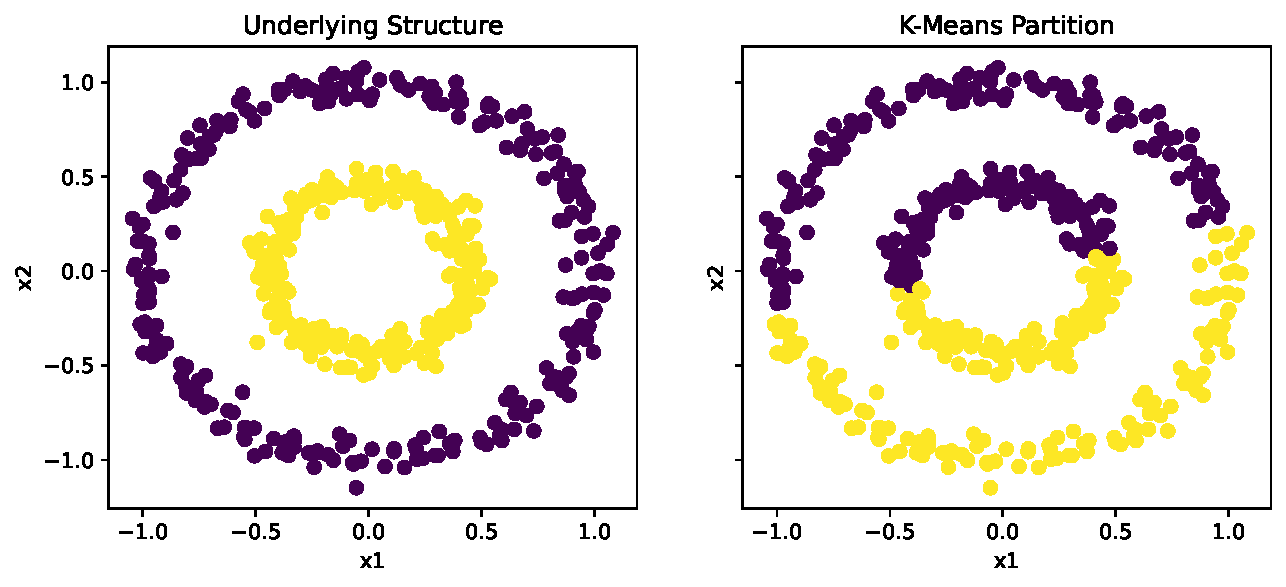
\includegraphics[keepaspectratio]{contents/3/cluster_files/figure-pdf/cell-16-output-1.pdf}}

K-means divides the feature space into convex regions, so it cannot
recover the two rings.

\section{Hierarchical: Agglomerative
Clustering}\label{hierarchical-agglomerative-clustering}

{Hierarchical} clustering builds a nested sequence of clusterings.
{Agglomerative} hierarchical clustering begins with each observation in
its own cluster and repeatedly merges the two ``closest'' clusters until
all observations belong to one cluster.

The result is a tree called a {\textbf{dendrogram}}. Unlike K-means, the
hierarchy can be fit before choosing the final number of clusters.

\subsection{Linkage}\label{linkage}

At each step of agglomerative hierarchical clustering, we merge the two
closest clusters. To determine which clusters are closest, we first need
to define the distance between clusters. A linkage rule specifies how
this distance is computed.

For two clusters \(G\) and \(H\), common linkage rules include:

\begin{itemize}
\tightlist
\item
  Single linkage uses the closest pair:
  \(d_{\text{single}}(G,H)=\min_{i\in G,\;j\in H}d(x_i,x_j).\)
\item
  Complete linkage uses the farthest pair:
  \(d_{\text{complete}}(G,H)=\max_{i\in G,\;j\in H}d(x_i,x_j).\)
\item
  Average linkage uses the average pairwise distance:
  \(d_{\text{avg}}(G,H)=\frac{1}{|G||H|}\sum_{i\in G,j\in H}d(x_i,x_j).\)
\item
  Ward linkage merges the pair of clusters that produces the smallest
  increase in the within-cluster sum of squares (WCSS). Unlike the
  previous linkage rules, Ward linkage is based on cluster variance
  rather than pairwise distances, and therefore tends to produce
  compact, approximately spherical clusters.
\end{itemize}

Different linkage rules represent different notions of what makes two
clusters close. Single linkage can recover elongated or irregularly
shaped clusters, but it is sensitive to the chaining effect, where
intermediate points connect otherwise separate groups. Complete linkage
and Ward linkage are less affected by chaining and tend to produce more
compact clusters.

\subsection{Dendrogram}\label{dendrogram}

A dendrogram is a visual record of the sequence of merges. At the
beginning, each observation is its own cluster. At each step, the two
closest current clusters are merged according to the chosen linkage
rule. The height of the merge records the dissimilarity at which the two
branches are joined.

The merge height is not always the distance between two individual
observations. It is the dissimilarity between the two clusters being
merged, as defined by the linkage rule. For single linkage, the height
is the smallest pairwise distance between the two clusters. For complete
linkage, it is the largest pairwise distance; for average linkage, it is
the average pairwise distance; and for Ward linkage, it is based on the
increase in within-cluster variation caused by the merge.

For example, consider five one-dimensional observations:

\[
0.0,\quad 0.2,\quad 0.3,\quad 3.0,\quad 3.2.
\]

Using single linkage, the tree is built as follows:

\begin{enumerate}
\def\labelenumi{\arabic{enumi}.}
\tightlist
\item
  Merge \(0.2\) and \(0.3\), the closest pair, at height \(0.1\).
\item
  Merge \(0.0\) with the cluster \(\{0.2,0.3\}\) at height \(0.2\).
\item
  Merge \(3.0\) and \(3.2\) at height \(0.2\).
\item
  Merge the two larger clusters \(\{0.0,0.2,0.3\}\) and \(\{3.0,3.2\}\)
  at height \(2.7\).
\end{enumerate}

\pandocbounded{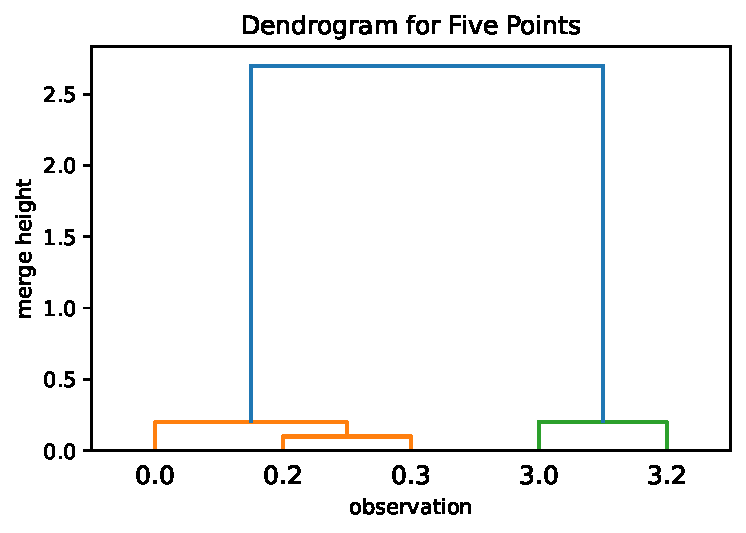
\includegraphics[keepaspectratio]{contents/3/cluster_files/figure-pdf/cell-17-output-1.pdf}}

The toy dendrogram shows the main interpretation: observations that
merge at low heights are similar under the chosen linkage rule, while
branches that merge only at high heights are more separated.

\subsection{Hierarchical clustering in
Python}\label{hierarchical-clustering-in-python}

In \texttt{sklearn}, agglomerative hierarchical clustering is fit using
\texttt{AgglomerativeClustering}. Here we apply it to the simulated
dataset from K-means. Like other \texttt{sklearn} estimators, it
provides \texttt{fit\_predict} for returning cluster assignments.

\begin{Shaded}
\begin{Highlighting}[]
\ImportTok{from}\NormalTok{ sklearn.cluster }\ImportTok{import}\NormalTok{ AgglomerativeClustering}
\NormalTok{hierarchical\_model }\OperatorTok{=}\NormalTok{ AgglomerativeClustering(n\_clusters}\OperatorTok{=}\DecValTok{3}\NormalTok{, linkage}\OperatorTok{=}\StringTok{"single"}\NormalTok{)}
\NormalTok{hierarchical\_cluster }\OperatorTok{=}\NormalTok{ hierarchical\_model.fit\_predict(X)}
\end{Highlighting}
\end{Shaded}

Here \texttt{n\_clusters=3} is chosen for illustration. We can visualize
the resulting cluster assignments in the original feature space.

\begin{Shaded}
\begin{Highlighting}[]
\ImportTok{import}\NormalTok{ matplotlib.pyplot }\ImportTok{as}\NormalTok{ plt}

\NormalTok{plt.scatter(X[:, }\DecValTok{0}\NormalTok{], X[:, }\DecValTok{1}\NormalTok{], c}\OperatorTok{=}\NormalTok{hierarchical\_cluster)}
\NormalTok{plt.xlabel(}\StringTok{"x1"}\NormalTok{)}
\NormalTok{plt.ylabel(}\StringTok{"x2"}\NormalTok{)}
\NormalTok{plt.title(}\StringTok{"Hierarchical Clustering Assignments"}\NormalTok{)}\OperatorTok{;}
\end{Highlighting}
\end{Shaded}

\pandocbounded{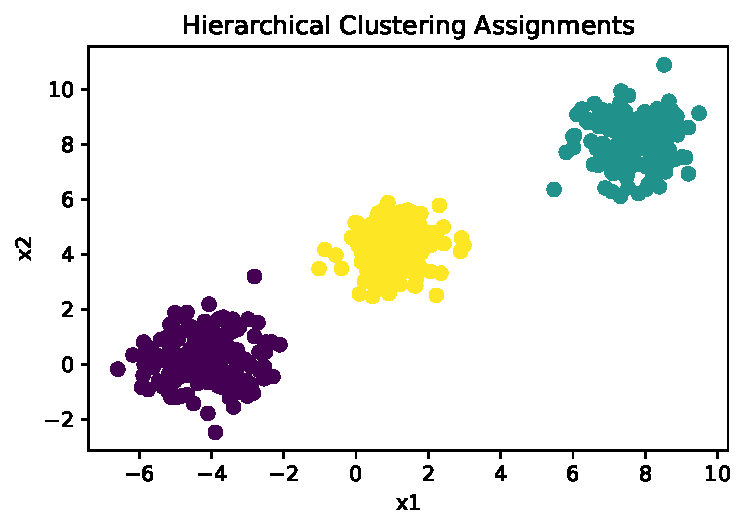
\includegraphics[keepaspectratio]{contents/3/cluster_files/figure-pdf/cell-19-output-1.pdf}}

\texttt{sklearn} can fit an agglomerative hierarchical clustering model
and return the cluster assignments, but it does not provide a function
to directly plot a dendrogram. For visualization, we use
\texttt{linkage} from \texttt{scipy.cluster.hierarchy} to compute the
hierarchy and \texttt{dendrogram} to display the resulting merge tree.

\begin{Shaded}
\begin{Highlighting}[]
\ImportTok{from}\NormalTok{ scipy.cluster.hierarchy }\ImportTok{import}\NormalTok{ linkage, dendrogram}

\NormalTok{Z }\OperatorTok{=}\NormalTok{ linkage(X, method}\OperatorTok{=}\StringTok{"single"}\NormalTok{)}
\NormalTok{dendrogram(Z)}
\NormalTok{plt.xlabel(}\StringTok{"observation"}\NormalTok{)}
\NormalTok{plt.ylabel(}\StringTok{"merge height"}\NormalTok{)}
\NormalTok{plt.title(}\StringTok{"Hierarchical Clustering Dendrogram"}\NormalTok{)}\OperatorTok{;}
\end{Highlighting}
\end{Shaded}

\pandocbounded{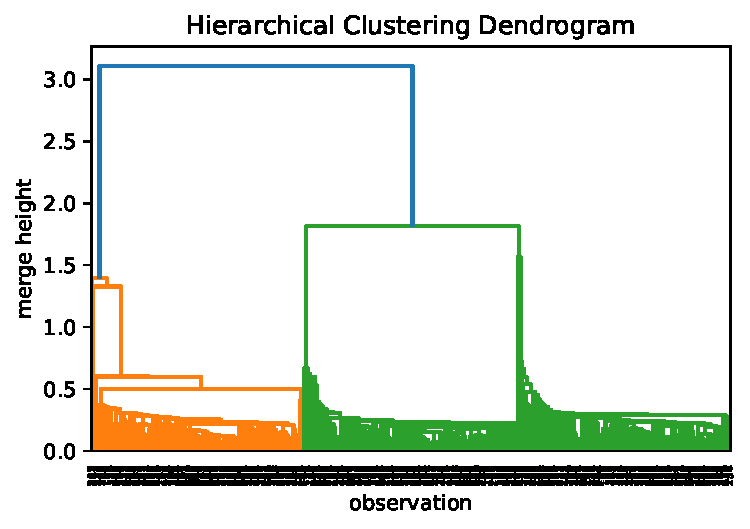
\includegraphics[keepaspectratio]{contents/3/cluster_files/figure-pdf/cell-20-output-1.pdf}}

The merge height records the dissimilarity at which two clusters are
merged. The dendrogram summarizes the fitted hierarchy, not uncertainty
about the hierarchy.

\begin{tcolorbox}[enhanced jigsaw, arc=.35mm, bottomrule=.15mm, bottomtitle=1mm, breakable, colback=white, colbacktitle=quarto-callout-note-color!10!white, colframe=quarto-callout-note-color-frame, coltitle=black, left=2mm, leftrule=.75mm, opacityback=0, opacitybacktitle=0.6, rightrule=.15mm, title=\textcolor{quarto-callout-note-color}{\faInfo}\hspace{0.5em}{Cutting the Dendrogram}, titlerule=0mm, toprule=.15mm, toptitle=1mm]

Hierarchical clustering separates fitting the hierarchy from choosing
the final flat clustering. One conceptual approach is to inspect the
dendrogram and make a horizontal cut at a merge height. This keeps
merges below the cut and separates branches that would only merge above
the cut.

The cut height is often chosen by looking for a large vertical gap in
the dendrogram, but this is only a heuristic. It should be checked
against the analysis goal, stability, validation scores, and
interpretability.

\end{tcolorbox}

\begin{tcolorbox}[enhanced jigsaw, arc=.35mm, bottomrule=.15mm, bottomtitle=1mm, breakable, colback=white, colbacktitle=quarto-callout-note-color!10!white, colframe=quarto-callout-note-color-frame, coltitle=black, left=2mm, leftrule=.75mm, opacityback=0, opacitybacktitle=0.6, rightrule=.15mm, title=\textcolor{quarto-callout-note-color}{\faInfo}\hspace{0.5em}{\texttt{n\_clusters} versus a height cut}, titlerule=0mm, toprule=.15mm, toptitle=1mm]

In \texttt{sklearn}, the usual
\texttt{AgglomerativeClustering(n\_clusters=...)} interface asks for an
exact number of clusters. This is not the same as drawing a horizontal
line at a fixed dendrogram height. The algorithm can return any
requested value of \texttt{n\_clusters}, even when several merges occur
at the same height. Operationally, this is equivalent to following the
merge sequence determined by the implementation and stopping when
exactly \texttt{n\_clusters} groups remain, rather than choosing all
merges below a fixed height. If several candidate merges have the same
height, the order is implementation-determined, not random.

If the goal is a strict height-based cut, use
\texttt{scipy.cluster.hierarchy.linkage} with \texttt{fcluster}, or use
\texttt{AgglomerativeClustering} with \texttt{distance\_threshold} and
\texttt{n\_clusters=None}. In this chapter, we focus mainly on the
\texttt{sklearn} \texttt{n\_clusters} interface because it is simple and
matches the way the examples compare flat cluster assignments.

\end{tcolorbox}

\subsection{Comparing Linkages}\label{comparing-linkages}

To make the effect of linkage visible, we use a dataset whose geometry
is not compact or spherical. The two-moons data have two curved groups,
so different linkage rules can produce noticeably different flat
clusterings.

Although the data are generated from two underlying groups, we set
\texttt{n\_clusters=4} here to make the behavior of the linkage rules
easier to compare.

\begin{Shaded}
\begin{Highlighting}[]
\ImportTok{from}\NormalTok{ sklearn.cluster }\ImportTok{import}\NormalTok{ AgglomerativeClustering}
\ImportTok{from}\NormalTok{ sklearn.datasets }\ImportTok{import}\NormalTok{ make\_moons}
\ImportTok{import}\NormalTok{ matplotlib.pyplot }\ImportTok{as}\NormalTok{ plt}

\NormalTok{X\_ex, \_ }\OperatorTok{=}\NormalTok{ make\_moons(n\_samples}\OperatorTok{=}\DecValTok{400}\NormalTok{, noise}\OperatorTok{=}\FloatTok{0.06}\NormalTok{, random\_state}\OperatorTok{=}\DecValTok{6}\NormalTok{)}

\NormalTok{methods }\OperatorTok{=}\NormalTok{ [}\StringTok{"single"}\NormalTok{, }\StringTok{"complete"}\NormalTok{, }\StringTok{"average"}\NormalTok{, }\StringTok{"ward"}\NormalTok{]}
\NormalTok{fig, axs }\OperatorTok{=}\NormalTok{ plt.subplots(}\DecValTok{2}\NormalTok{, }\DecValTok{2}\NormalTok{, figsize}\OperatorTok{=}\NormalTok{(}\DecValTok{10}\NormalTok{, }\DecValTok{8}\NormalTok{), sharex}\OperatorTok{=}\VariableTok{True}\NormalTok{, sharey}\OperatorTok{=}\VariableTok{True}\NormalTok{)}

\ControlFlowTok{for}\NormalTok{ ax, method }\KeywordTok{in} \BuiltInTok{zip}\NormalTok{(axs.ravel(), methods):}
\NormalTok{    model }\OperatorTok{=}\NormalTok{ AgglomerativeClustering(n\_clusters}\OperatorTok{=}\DecValTok{4}\NormalTok{, linkage}\OperatorTok{=}\NormalTok{method)}
\NormalTok{    labels }\OperatorTok{=}\NormalTok{ model.fit\_predict(X\_ex)}

\NormalTok{    ax.scatter(X\_ex[:, }\DecValTok{0}\NormalTok{], X\_ex[:, }\DecValTok{1}\NormalTok{], c}\OperatorTok{=}\NormalTok{labels)}
\NormalTok{    ax.set\_title(method)}
\NormalTok{    ax.set\_xlabel(}\StringTok{"x1"}\NormalTok{)}
\NormalTok{    ax.set\_ylabel(}\StringTok{"x2"}\NormalTok{)}\OperatorTok{;}
\end{Highlighting}
\end{Shaded}

\pandocbounded{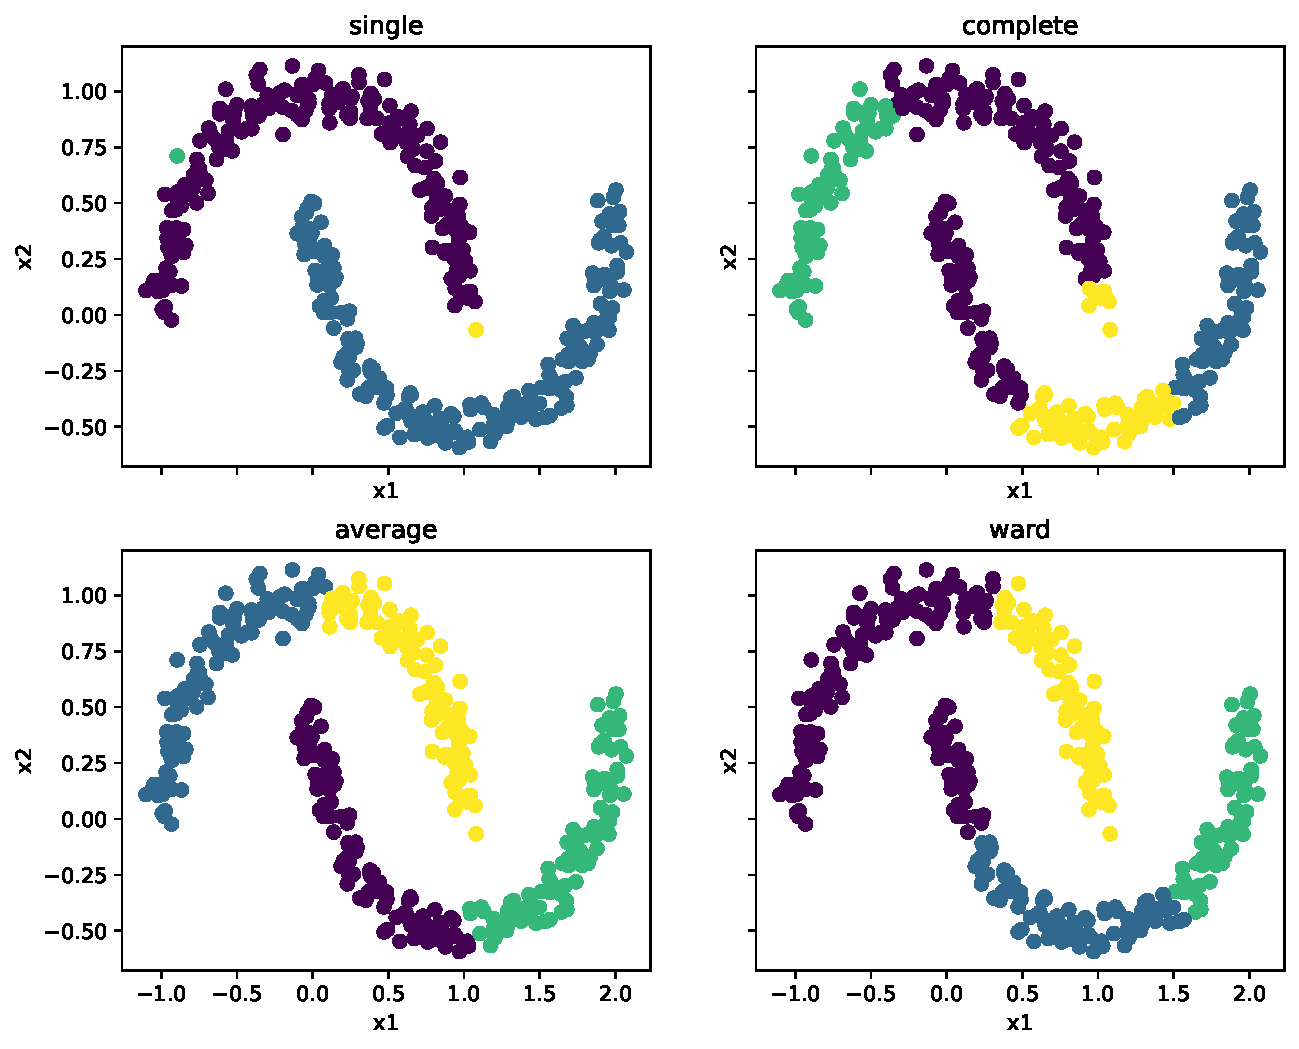
\includegraphics[keepaspectratio]{contents/3/cluster_files/figure-pdf/cell-21-output-1.pdf}}

The cluster labels are arbitrary, so the important feature is the shape
of the split:

\begin{itemize}
\tightlist
\item
  Single linkage uses the closest pair of observations between two
  clusters. It favors connected shapes and can follow long curves. In
  the plot, it keeps most of each moon as a connected chain, and the
  extra clusters appear where a small gap breaks the chain.
\item
  Complete linkage uses the farthest pair of observations between two
  clusters. It favors clusters with small diameter, so it tends to
  produce compact, ball-like groups rather than long or stretched
  groups. In the plot, it cuts the moons into shorter pieces instead of
  preserving the full curved shapes.
\item
  Average linkage uses the average distance over all pairs of
  observations between two clusters. It is a compromise between
  connectivity and compactness: it is less sensitive to one nearby pair
  than single linkage, but less strict about the farthest pair than
  complete linkage. In the plot, it still splits the moons where the
  average distance to the rest of the arc becomes large.
\item
  Ward linkage merges clusters that cause the smallest increase in WCSS.
  It favors compact, variance-minimizing clusters, similar in spirit to
  K-means. In the plot, its cuts look like local spatial blocks rather
  than moon-shaped pieces, because the curved groups are not compact
  around a single center.
\end{itemize}

\begin{tcolorbox}[enhanced jigsaw, arc=.35mm, bottomrule=.15mm, bottomtitle=1mm, breakable, colback=white, colbacktitle=quarto-callout-note-color!10!white, colframe=quarto-callout-note-color-frame, coltitle=black, left=2mm, leftrule=.75mm, opacityback=0, opacitybacktitle=0.6, rightrule=.15mm, title=\textcolor{quarto-callout-note-color}{\faInfo}\hspace{0.5em}{Complete linkage and Ward linkage}, titlerule=0mm, toprule=.15mm, toptitle=1mm]

Complete linkage and Ward linkage both tend to produce compact,
ball-like clusters, but they measure compactness differently.

\begin{itemize}
\tightlist
\item
  Complete linkage is based on cluster diameter. It avoids merges that
  would make the farthest two observations in a cluster too far apart.
\item
  Ward linkage is based on within-cluster variation. It avoids merges
  that would cause a large increase in WCSS, where each cluster is
  summarized by its mean.
\end{itemize}

Thus, complete linkage is diameter-based compactness, while Ward linkage
is variance-based compactness.

They can differ when cluster sizes or shapes are uneven. Complete
linkage reacts strongly to the most distant pair of observations, so one
outlying point can prevent a merge by making the cluster diameter too
large. Ward linkage reacts to the overall increase in WCSS, so it also
depends on cluster sizes and centroids. If two large clusters have
nearby centers, Ward linkage may still merge them even when a few
observations are relatively far apart, because those observations may
not dominate the total WCSS increase.

\end{tcolorbox}

\subsection{When Hierarchical Clustering Works
Well}\label{when-hierarchical-clustering-works-well}

Hierarchical clustering is especially useful when the nested structure
itself is meaningful. For example, it is often used to organize genes,
documents, products, or other observations where relationships at
multiple levels of granularity are informative.

It is most useful when:

\begin{itemize}
\tightlist
\item
  the hierarchy itself is part of the interpretation;
\item
  one wants to inspect several possible numbers of clusters from the
  same fitted tree;
\item
  the dataset is small or moderate in size;
\item
  the chosen linkage rule matches the geometry of the groups.
\end{itemize}

However, agglomerative clustering can be computationally expensive for
very large datasets, and early merges cannot be undone. A suboptimal
early merge can affect the rest of the tree.

\section{Density-Based: DBSCAN}\label{density-based-dbscan}

Density-based spatial clustering of applications with noise (DBSCAN)
defines clusters as connected regions of sufficiently high local
density. Unlike K-means or hierarchical clustering, DBSCAN does not
require the number of clusters to be specified in advance.

The main idea is that a cluster should be a dense region separated from
other dense regions by lower-density space. This makes DBSCAN useful
when clusters are curved, irregularly shaped, or when some observations
should be treated as noise rather than forced into a cluster.

DBSCAN uses two main parameters:

\begin{itemize}
\tightlist
\item
  \texttt{eps}: the radius of a local neighborhood;
\item
  \texttt{min\_samples}: the number of observations required for a dense
  neighborhood, including the observation itself.
\end{itemize}

These parameters define three types of observations:

\begin{itemize}
\tightlist
\item
  A \textbf{core point} has at least \texttt{min\_samples} observations
  in its \texttt{eps} neighborhood, including itself.
\item
  A \textbf{border point} is not a core point, but lies within the
  \texttt{eps} neighborhood of a core point.
\item
  A \textbf{noise point} is neither a core point nor a border point.
\end{itemize}

\subsection{How DBSCAN Forms Clusters}\label{how-dbscan-forms-clusters}

DBSCAN begins by checking the \texttt{eps} neighborhood of each
observation. If an observation has at least \texttt{min\_samples}
observations in that neighborhood, counting itself, it becomes a core
point. A core point can start a new cluster if it has not already been
reached from another core point.

Once a core point starts a cluster, DBSCAN adds all observations within
its \texttt{eps} neighborhood. If any of those observations are also
core points, their own \texttt{eps} neighborhoods are added as well.
This expansion continues until no new core points can be reached. All
core points connected in this way belong to the same cluster, and
non-core points reached from those core points are included as border
points.

Observations that are not reachable from any core point are labeled as
noise. Thus, DBSCAN does not assign points by nearest center. It forms
clusters by following chains of dense neighborhoods, and the number of
clusters is whatever number of separated dense regions the algorithm
finds.

\subsection{DBSCAN in Python}\label{dbscan-in-python}

We use \texttt{DBSCAN} from \texttt{sklearn.cluster} to implement the
method.

\begin{Shaded}
\begin{Highlighting}[]
\ImportTok{from}\NormalTok{ sklearn.cluster }\ImportTok{import}\NormalTok{ DBSCAN}
\ImportTok{from}\NormalTok{ sklearn.datasets }\ImportTok{import}\NormalTok{ make\_circles}


\NormalTok{X\_circle, true\_circle\_group }\OperatorTok{=}\NormalTok{ make\_circles(}
\NormalTok{    n\_samples}\OperatorTok{=}\DecValTok{500}\NormalTok{, factor}\OperatorTok{=}\FloatTok{0.45}\NormalTok{, noise}\OperatorTok{=}\FloatTok{0.05}\NormalTok{, random\_state}\OperatorTok{=}\DecValTok{1}
\NormalTok{)}

\NormalTok{circle\_dbscan }\OperatorTok{=}\NormalTok{ DBSCAN(eps}\OperatorTok{=}\FloatTok{0.13}\NormalTok{, min\_samples}\OperatorTok{=}\DecValTok{4}\NormalTok{)}
\NormalTok{circle\_dbscan\_group }\OperatorTok{=}\NormalTok{ circle\_dbscan.fit\_predict(X\_circle)}
\end{Highlighting}
\end{Shaded}

\begin{Shaded}
\begin{Highlighting}[]
\ImportTok{import}\NormalTok{ matplotlib.pyplot }\ImportTok{as}\NormalTok{ plt}

\NormalTok{fig, axs }\OperatorTok{=}\NormalTok{ plt.subplots(}\DecValTok{1}\NormalTok{, }\DecValTok{2}\NormalTok{, figsize}\OperatorTok{=}\NormalTok{(}\DecValTok{10}\NormalTok{, }\DecValTok{4}\NormalTok{), sharex}\OperatorTok{=}\VariableTok{True}\NormalTok{, sharey}\OperatorTok{=}\VariableTok{True}\NormalTok{)}

\NormalTok{axs[}\DecValTok{0}\NormalTok{].scatter(X\_circle[:, }\DecValTok{0}\NormalTok{], X\_circle[:, }\DecValTok{1}\NormalTok{], c}\OperatorTok{=}\NormalTok{circle\_cluster)}
\NormalTok{axs[}\DecValTok{0}\NormalTok{].set\_title(}\StringTok{"K{-}Means"}\NormalTok{)}

\NormalTok{axs[}\DecValTok{1}\NormalTok{].scatter(X\_circle[:, }\DecValTok{0}\NormalTok{], X\_circle[:, }\DecValTok{1}\NormalTok{], c}\OperatorTok{=}\NormalTok{circle\_dbscan\_group)}
\NormalTok{axs[}\DecValTok{1}\NormalTok{].set\_title(}\StringTok{"DBSCAN"}\NormalTok{)}

\ControlFlowTok{for}\NormalTok{ ax }\KeywordTok{in}\NormalTok{ axs:}
\NormalTok{    ax.set\_xlabel(}\StringTok{"x1"}\NormalTok{)}
\NormalTok{    ax.set\_ylabel(}\StringTok{"x2"}\NormalTok{)}
\end{Highlighting}
\end{Shaded}

\pandocbounded{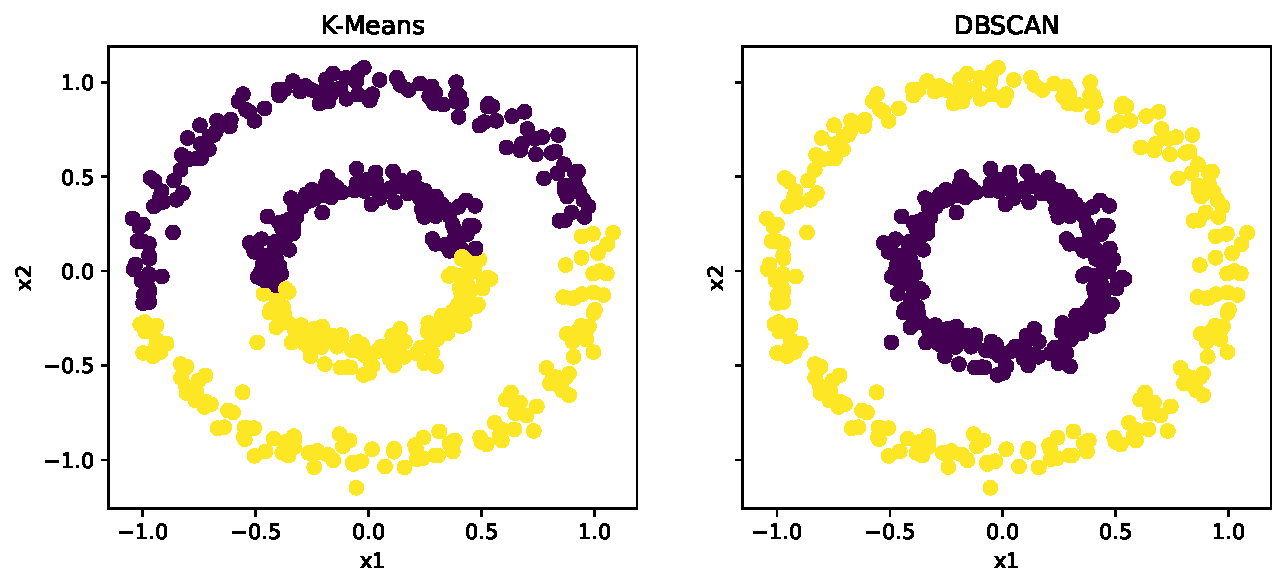
\includegraphics[keepaspectratio]{contents/3/cluster_files/figure-pdf/cell-23-output-1.pdf}}

In \texttt{sklearn}, noise observations receive the label \texttt{-1}.
As with all clustering labels, the nonnegative cluster labels have no
ordinal meaning.

\subsection{\texorpdfstring{Choosing \texttt{eps} and
\texttt{min\_samples}}{Choosing eps and min\_samples}}\label{choosing-eps-and-min_samples}

The most important DBSCAN hyperparameter is \texttt{eps}, because it
controls the scale at which density is measured. A smaller \texttt{eps}
makes neighborhoods smaller and the density requirement stricter. This
may split clusters or label more observations as noise. A larger
\texttt{eps} makes neighborhoods larger and can merge groups through
low-density bridges.

The parameter \texttt{min\_samples} controls how much local support is
required for a point to be considered a core point. Larger values make
the method more conservative and usually produce more noise points.

A practical workflow is to first set \texttt{min\_samples}, then use the
data to select \texttt{eps}. A common starting choice is to set
\texttt{min\_samples} to about twice the number of features. In this
two-dimensional example, we use \texttt{4}.

\begin{tcolorbox}[enhanced jigsaw, arc=.35mm, bottomrule=.15mm, bottomtitle=1mm, breakable, colback=white, colbacktitle=quarto-callout-note-color!10!white, colframe=quarto-callout-note-color-frame, coltitle=black, left=2mm, leftrule=.75mm, opacityback=0, opacitybacktitle=0.6, rightrule=.15mm, title=\textcolor{quarto-callout-note-color}{\faInfo}\hspace{0.5em}{Checking \texttt{min\_samples}}, titlerule=0mm, toprule=.15mm, toptitle=1mm]

There is no supervised-style cross-validation rule for choosing
\texttt{min\_samples}. A reasonable value should give a stable and
interpretable density structure: nearby choices should not radically
change the main clusters, and the fraction of noise points should be
plausible for the problem. A lower noise fraction is not automatically
better, because forcing sparse points into clusters may hide outliers or
connect groups through weak bridges.

Several diagnostics can help. For a chosen \texttt{min\_samples}, the
k-distance plot should ideally show a reasonably clear elbow, suggesting
a defensible density scale. As a starting point, two-dimensional data
often use \texttt{min\_samples=4} or \texttt{5}; more generally, one may
start around \texttt{p\ +\ 1} or \texttt{2p}, where \(p\) is the number
of features.

If external labels are available, the Rand index or adjusted Rand index
can be used as additional diagnostics.

\end{tcolorbox}

After choosing \texttt{min\_samples}, compute the distance from each
observation to the neighbor that determines whether it is a core point.
Since \texttt{min\_samples} includes the observation itself in
\texttt{sklearn}, this is the distance to the \texttt{min\_samples}-th
nearest observation when the observation itself is included as the first
neighbor. Points inside dense regions should have small such distances,
while isolated or low-density points should have larger distances.
Sorting these distances gives a diagnostic plot. A visible elbow in the
plot suggests a candidate value of \texttt{eps}.

In Python we can use \texttt{NearestNeighbors} from
\texttt{sklearn.neighbors} to compute these distances. The result is
then sorted and plotted.

\begin{Shaded}
\begin{Highlighting}[]
\ImportTok{from}\NormalTok{ sklearn.neighbors }\ImportTok{import}\NormalTok{ NearestNeighbors}

\NormalTok{min\_samples }\OperatorTok{=} \DecValTok{4}

\NormalTok{neighbors }\OperatorTok{=}\NormalTok{ NearestNeighbors(n\_neighbors}\OperatorTok{=}\NormalTok{min\_samples)}
\NormalTok{neighbors.fit(X\_circle)}

\NormalTok{distances, indices }\OperatorTok{=}\NormalTok{ neighbors.kneighbors(X\_circle)}
\NormalTok{k\_distances }\OperatorTok{=}\NormalTok{ np.sort(distances[:, }\OperatorTok{{-}}\DecValTok{1}\NormalTok{])}

\NormalTok{plt.plot(k\_distances)}
\NormalTok{plt.axhline(y}\OperatorTok{=}\FloatTok{0.13}\NormalTok{, ls}\OperatorTok{=}\StringTok{"{-}{-}"}\NormalTok{)}
\NormalTok{plt.xlabel(}\StringTok{"sorted observation index"}\NormalTok{)}
\NormalTok{plt.ylabel(}\SpecialStringTok{f"distance to }\SpecialCharTok{\{}\NormalTok{min\_samples}\SpecialCharTok{\}}\SpecialStringTok{{-}th nearest neighbor"}\NormalTok{)}
\NormalTok{plt.title(}\StringTok{"K{-}Distance Plot for Choosing eps"}\NormalTok{)}\OperatorTok{;}
\end{Highlighting}
\end{Shaded}

\pandocbounded{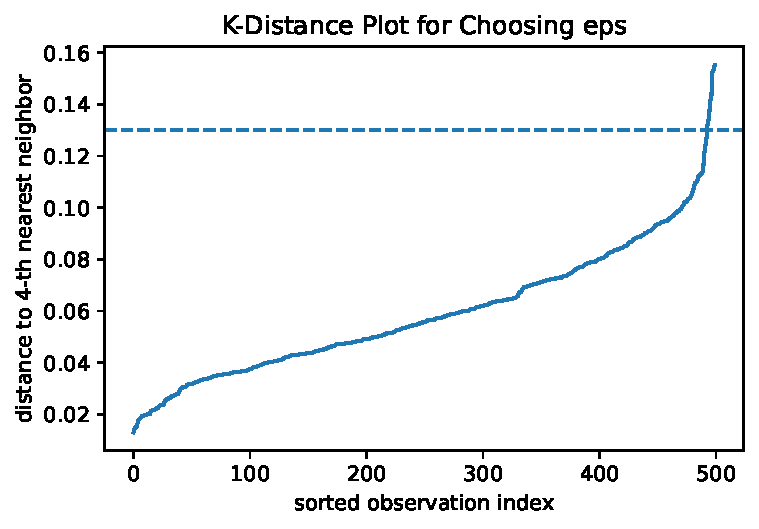
\includegraphics[keepaspectratio]{contents/3/cluster_files/figure-pdf/cell-24-output-1.pdf}}

A candidate \texttt{eps} can be drawn as a horizontal line on this plot.
Observations with k-distances below the line satisfy the core-point
density requirement. Observations above the line are not core points;
they may later become border points if they lie within \texttt{eps} of a
core point, or they may be labeled as noise.

Thus, decreasing \texttt{eps} usually creates fewer core points, more
noise, and a greater chance that a dense region is split into pieces.
Increasing \texttt{eps} usually creates more core points and a greater
chance that nearby dense regions are merged through a bridge of points.

In this example, the curve remains relatively flat for most observations
and then increases more sharply for observations whose local
neighborhoods are sparser. An \texttt{eps} value near the bend separates
the dense ring structure from the lower-density gaps. We next check
nearby values.

\begin{Shaded}
\begin{Highlighting}[]
\NormalTok{eps\_values }\OperatorTok{=}\NormalTok{ [}\FloatTok{0.12}\NormalTok{, }\FloatTok{0.13}\NormalTok{, }\FloatTok{0.14}\NormalTok{]}

\NormalTok{fig, axs }\OperatorTok{=}\NormalTok{ plt.subplots(}\DecValTok{1}\NormalTok{, }\DecValTok{3}\NormalTok{, figsize}\OperatorTok{=}\NormalTok{(}\DecValTok{12}\NormalTok{, }\DecValTok{4}\NormalTok{), sharex}\OperatorTok{=}\VariableTok{True}\NormalTok{, sharey}\OperatorTok{=}\VariableTok{True}\NormalTok{)}

\ControlFlowTok{for}\NormalTok{ ax, eps }\KeywordTok{in} \BuiltInTok{zip}\NormalTok{(axs, eps\_values):}
\NormalTok{    labels }\OperatorTok{=}\NormalTok{ DBSCAN(eps}\OperatorTok{=}\NormalTok{eps, min\_samples}\OperatorTok{=}\NormalTok{min\_samples).fit\_predict(X\_circle)}

\NormalTok{    ax.scatter(X\_circle[:, }\DecValTok{0}\NormalTok{], X\_circle[:, }\DecValTok{1}\NormalTok{], c}\OperatorTok{=}\NormalTok{labels)}
\NormalTok{    ax.set\_title(}\SpecialStringTok{f"eps = }\SpecialCharTok{\{}\NormalTok{eps}\SpecialCharTok{\}}\SpecialStringTok{"}\NormalTok{)}
\NormalTok{    ax.set\_xlabel(}\StringTok{"x1"}\NormalTok{)}
\NormalTok{    ax.set\_ylabel(}\StringTok{"x2"}\NormalTok{)}
\end{Highlighting}
\end{Shaded}

\pandocbounded{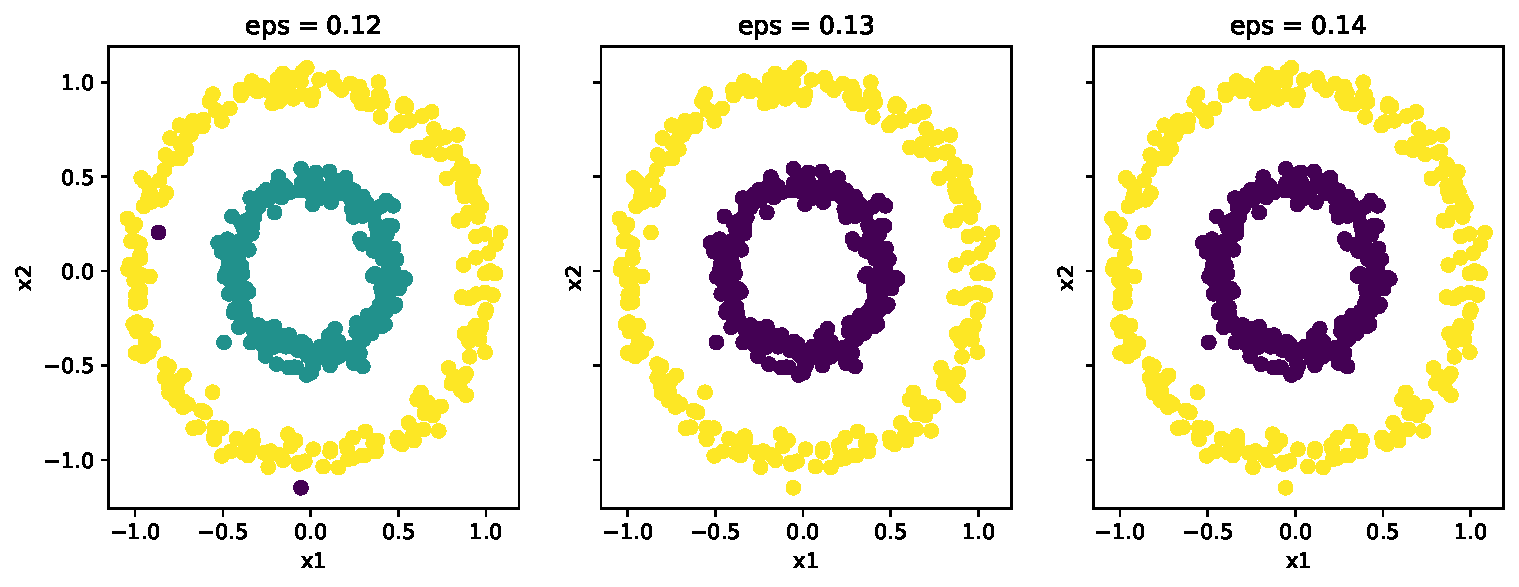
\includegraphics[keepaspectratio]{contents/3/cluster_files/figure-pdf/cell-25-output-1.pdf}}

If small changes in \texttt{eps} lead to very different cluster
assignments, the density structure may not be stable at a single scale.
In that case, the fitted clusters should be interpreted cautiously, or a
method designed for varying density levels may be more appropriate.

In this example, from \texttt{0.12} to \texttt{0.14} the clustering
structure is relatively stable. The color labels may change because
cluster labels are arbitrary, but the two-ring grouping is essentially
the same. Therefore, \texttt{0.13} is a reasonable choice within this
stable range.

\begin{tcolorbox}[enhanced jigsaw, arc=.35mm, bottomrule=.15mm, bottomtitle=1mm, breakable, colback=white, colbacktitle=quarto-callout-caution-color!10!white, colframe=quarto-callout-caution-color-frame, coltitle=black, left=2mm, leftrule=.75mm, opacityback=0, opacitybacktitle=0.6, rightrule=.15mm, title=\textcolor{quarto-callout-caution-color}{\faFire}\hspace{0.5em}{Silhouette scores are only a rough diagnostic for DBSCAN}, titlerule=0mm, toprule=.15mm, toptitle=1mm]

One can compute silhouette scores over a grid of \texttt{eps} and
\texttt{min\_samples} values, but this is not ordinary cross-validation
because clustering has no supervised prediction error. The score is also
harder to interpret for DBSCAN: treating noise as an extra cluster can
distort the score, while removing noise ignores one of DBSCAN's main
outputs.

Silhouette scores also favor compact, well-separated groups, whereas
DBSCAN is often used for curved or irregular clusters. Use them only as
a secondary diagnostic alongside the k-distance plot, the number of
clusters, the fraction of noise points, visual inspection when possible,
and sensitivity to nearby parameter values.

\end{tcolorbox}

\begin{tcolorbox}[enhanced jigsaw, arc=.35mm, bottomrule=.15mm, bottomtitle=1mm, breakable, colback=white, colbacktitle=quarto-callout-note-color!10!white, colframe=quarto-callout-note-color-frame, coltitle=black, left=2mm, leftrule=.75mm, opacityback=0, opacitybacktitle=0.6, rightrule=.15mm, title=\textcolor{quarto-callout-note-color}{\faInfo}\hspace{0.5em}{DBSCAN does not tune \texttt{n\_clusters}}, titlerule=0mm, toprule=.15mm, toptitle=1mm]

DBSCAN determines the number of clusters from the density structure
induced by \texttt{eps} and \texttt{min\_samples}. This is useful when
the number of groups is unknown, but it also means that the result can
change substantially when the density scale changes.

\end{tcolorbox}

\subsection{When DBSCAN Works Well}\label{when-dbscan-works-well}

DBSCAN is most useful when:

\begin{itemize}
\tightlist
\item
  clusters have irregular or curved shapes;
\item
  clusters are separated by sparse regions;
\item
  noise points should be explicitly identified;
\item
  a single density scale is reasonable for the dataset.
\end{itemize}

It is less effective when cluster densities differ substantially. One
global value of \texttt{eps} may be too small for a sparse cluster and
too large for a dense cluster.

\section{Comparing the Three Methods}\label{comparing-the-three-methods}

The three direct methods answer different versions of the clustering
question. The key difference is their definitions of a cluster: what
each method treats as evidence that observations belong together:

{\def\LTcaptype{none} % do not increment counter
\begin{longtable}[]{@{}
  >{\raggedright\arraybackslash}p{(\linewidth - 4\tabcolsep) * \real{0.3333}}
  >{\raggedright\arraybackslash}p{(\linewidth - 4\tabcolsep) * \real{0.3333}}
  >{\raggedright\arraybackslash}p{(\linewidth - 4\tabcolsep) * \real{0.3333}}@{}}
\toprule\noalign{}
\begin{minipage}[b]{\linewidth}\raggedright
Method
\end{minipage} & \begin{minipage}[b]{\linewidth}\raggedright
Informal rule
\end{minipage} & \begin{minipage}[b]{\linewidth}\raggedright
Works especially well when
\end{minipage} \\
\midrule\noalign{}
\endhead
\bottomrule\noalign{}
\endlastfoot
K-means & Points belong together if they are close to the same center. &
clusters are roughly spherical, compact, and similar in size \\
Hierarchical clustering & Points belong together if they are joined
through a sequence of merges. & one wants to explore grouping structure
at several resolutions \\
DBSCAN & Points belong together if they lie in the same sufficiently
dense region. & clusters are dense regions, noise is present, and the
number of clusters is unknown \\
\end{longtable}
}

No method is uniformly best. The geometry of the data, the intended
definition of a cluster, and the scientific question should determine
which paradigm is appropriate. A useful comparison does not require
every method to look successful; a poor-looking fit can be informative
when it reveals the method's assumptions.

\begin{itemize}
\tightlist
\item
  K-means is fast, simple, and often the practical default when \(K\) is
  known and clusters are roughly compact and center-based. It can revise
  assignments during iteration, but it forces every observation into one
  of the \(K\) clusters and is not designed for curved shapes or
  explicit noise.
\item
  Agglomerative hierarchical clustering is most useful when the merge
  sequence or dendrogram is part of the interpretation. It can show
  several possible resolutions from one fitted tree, but early merges
  cannot be undone and classical agglomerative methods scale poorly
  because they rely on many pairwise dissimilarities.
\item
  DBSCAN is useful when clusters are dense regions separated by sparse
  space. It does not require \texttt{n\_clusters} and can label
  observations as noise, but it is sensitive to the density scale set by
  \texttt{eps} and \texttt{min\_samples} and does not show nested
  structure.
\end{itemize}

We show three examples below illustrating the strengths and limitations
of each method. These examples are not a ranking. They show that each
method is answering a different question: nearest center, merge tree, or
density connectivity. In the examples, the hierarchical clustering
result uses single linkage. When a method performs poorly on a
particular geometry, the failure is still useful if it matches the
method's definition of a cluster.

Since all datasets are generated, we know the true label for each
observation. Therefore, we can use ARI as an external metric to compare
the clustering results on each dataset. ARI is optional and was
introduced earlier in the notes.

In the curves-with-noise example, the artificially added noise points
are treated as a separate reference group when computing ARI. This is a
teaching device for simulated data, not something usually available in
real applications. It favors methods that can identify noise points,
such as DBSCAN, and penalizes methods such as K-means and hierarchical
clustering that must assign every observation to a cluster.

\subsection{Example: Curves with Noise}\label{example-curves-with-noise}

\begin{Shaded}
\begin{Highlighting}[]
\ImportTok{from}\NormalTok{ sklearn.datasets }\ImportTok{import}\NormalTok{ make\_blobs, make\_moons}
\ImportTok{from}\NormalTok{ sklearn.cluster }\ImportTok{import}\NormalTok{ KMeans, AgglomerativeClustering, DBSCAN}
\ImportTok{from}\NormalTok{ sklearn.metrics }\ImportTok{import}\NormalTok{ adjusted\_rand\_score}
\ImportTok{import}\NormalTok{ numpy }\ImportTok{as}\NormalTok{ np}
\ImportTok{import}\NormalTok{ matplotlib.pyplot }\ImportTok{as}\NormalTok{ plt}

\NormalTok{rng }\OperatorTok{=}\NormalTok{ np.random.default\_rng(}\DecValTok{2}\NormalTok{)}

\NormalTok{X\_moon, true\_moon\_group }\OperatorTok{=}\NormalTok{ make\_moons(n\_samples}\OperatorTok{=}\DecValTok{450}\NormalTok{, noise}\OperatorTok{=}\FloatTok{0.06}\NormalTok{, random\_state}\OperatorTok{=}\DecValTok{2}\NormalTok{)}
\NormalTok{moon\_noise }\OperatorTok{=}\NormalTok{ rng.uniform(low}\OperatorTok{=}\NormalTok{[}\OperatorTok{{-}}\FloatTok{1.5}\NormalTok{, }\OperatorTok{{-}}\FloatTok{0.8}\NormalTok{], high}\OperatorTok{=}\NormalTok{[}\FloatTok{2.5}\NormalTok{, }\FloatTok{1.3}\NormalTok{], size}\OperatorTok{=}\NormalTok{(}\DecValTok{30}\NormalTok{, }\DecValTok{2}\NormalTok{))}
\NormalTok{X\_moon\_noise }\OperatorTok{=}\NormalTok{ np.vstack([X\_moon, moon\_noise])}
\NormalTok{true\_moon\_noise\_group }\OperatorTok{=}\NormalTok{ np.concatenate(}
\NormalTok{    [true\_moon\_group, np.repeat(}\OperatorTok{{-}}\DecValTok{1}\NormalTok{, }\BuiltInTok{len}\NormalTok{(moon\_noise))]}
\NormalTok{)}

\NormalTok{kmeans\_labels }\OperatorTok{=}\NormalTok{ KMeans(n\_clusters}\OperatorTok{=}\DecValTok{2}\NormalTok{, n\_init}\OperatorTok{=}\DecValTok{20}\NormalTok{, random\_state}\OperatorTok{=}\DecValTok{1}\NormalTok{).fit\_predict(}
\NormalTok{    X\_moon\_noise}
\NormalTok{)}

\NormalTok{single\_labels }\OperatorTok{=}\NormalTok{ AgglomerativeClustering(n\_clusters}\OperatorTok{=}\DecValTok{2}\NormalTok{, linkage}\OperatorTok{=}\StringTok{"single"}\NormalTok{).fit\_predict(}
\NormalTok{    X\_moon\_noise}
\NormalTok{)}

\NormalTok{dbscan\_labels }\OperatorTok{=}\NormalTok{ DBSCAN(eps}\OperatorTok{=}\FloatTok{0.16}\NormalTok{, min\_samples}\OperatorTok{=}\DecValTok{6}\NormalTok{).fit\_predict(X\_moon\_noise)}

\NormalTok{kmeans\_ari }\OperatorTok{=}\NormalTok{ adjusted\_rand\_score(true\_moon\_noise\_group, kmeans\_labels)}
\NormalTok{single\_ari }\OperatorTok{=}\NormalTok{ adjusted\_rand\_score(true\_moon\_noise\_group, single\_labels)}
\NormalTok{dbscan\_ari }\OperatorTok{=}\NormalTok{ adjusted\_rand\_score(true\_moon\_noise\_group, dbscan\_labels)}

\NormalTok{fig, axs }\OperatorTok{=}\NormalTok{ plt.subplots(}\DecValTok{1}\NormalTok{, }\DecValTok{3}\NormalTok{, figsize}\OperatorTok{=}\NormalTok{(}\DecValTok{12}\NormalTok{, }\FloatTok{3.5}\NormalTok{), sharex}\OperatorTok{=}\VariableTok{False}\NormalTok{, sharey}\OperatorTok{=}\VariableTok{False}\NormalTok{)}

\NormalTok{axs[}\DecValTok{0}\NormalTok{].scatter(X\_moon\_noise[:, }\DecValTok{0}\NormalTok{], X\_moon\_noise[:, }\DecValTok{1}\NormalTok{], c}\OperatorTok{=}\NormalTok{kmeans\_labels, s}\OperatorTok{=}\DecValTok{16}\NormalTok{)}
\NormalTok{axs[}\DecValTok{0}\NormalTok{].set\_title(}\SpecialStringTok{f"K{-}Means}\CharTok{\textbackslash{}n}\SpecialStringTok{ARI = }\SpecialCharTok{\{}\NormalTok{kmeans\_ari}\SpecialCharTok{:.2f\}}\SpecialStringTok{"}\NormalTok{)}

\NormalTok{axs[}\DecValTok{1}\NormalTok{].scatter(X\_moon\_noise[:, }\DecValTok{0}\NormalTok{], X\_moon\_noise[:, }\DecValTok{1}\NormalTok{], c}\OperatorTok{=}\NormalTok{single\_labels, s}\OperatorTok{=}\DecValTok{16}\NormalTok{)}
\NormalTok{axs[}\DecValTok{1}\NormalTok{].set\_title(}\SpecialStringTok{f"Hierarchical: Single}\CharTok{\textbackslash{}n}\SpecialStringTok{ARI = }\SpecialCharTok{\{}\NormalTok{single\_ari}\SpecialCharTok{:.2f\}}\SpecialStringTok{"}\NormalTok{)}

\NormalTok{axs[}\DecValTok{2}\NormalTok{].scatter(X\_moon\_noise[:, }\DecValTok{0}\NormalTok{], X\_moon\_noise[:, }\DecValTok{1}\NormalTok{], c}\OperatorTok{=}\NormalTok{dbscan\_labels, s}\OperatorTok{=}\DecValTok{16}\NormalTok{)}
\NormalTok{axs[}\DecValTok{2}\NormalTok{].set\_title(}\SpecialStringTok{f"DBSCAN}\CharTok{\textbackslash{}n}\SpecialStringTok{ARI = }\SpecialCharTok{\{}\NormalTok{dbscan\_ari}\SpecialCharTok{:.2f\}}\SpecialStringTok{"}\NormalTok{)}

\ControlFlowTok{for}\NormalTok{ ax }\KeywordTok{in}\NormalTok{ axs:}
\NormalTok{    ax.set\_xlabel(}\StringTok{"x1"}\NormalTok{)}
\NormalTok{    ax.set\_ylabel(}\StringTok{"x2"}\NormalTok{)}

\NormalTok{fig.suptitle(}\StringTok{"Curves with Noise"}\NormalTok{, y}\OperatorTok{=}\FloatTok{1.05}\NormalTok{)}\OperatorTok{;}
\end{Highlighting}
\end{Shaded}

\pandocbounded{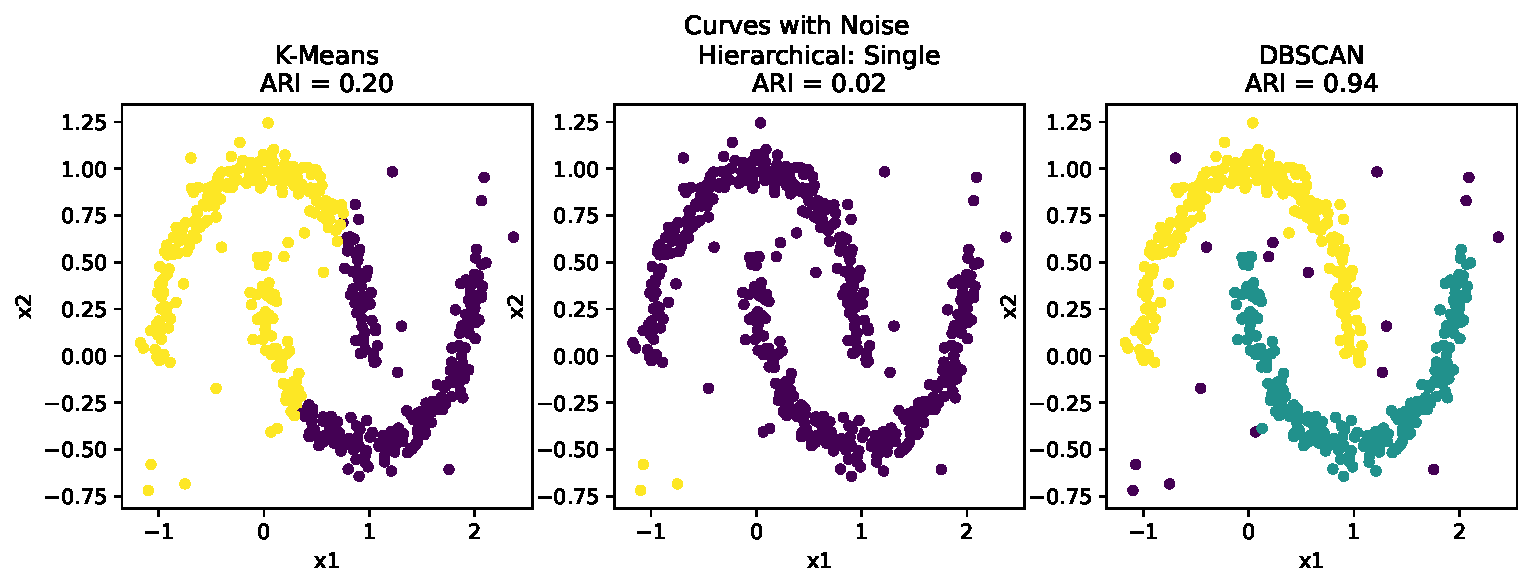
\includegraphics[keepaspectratio]{contents/3/cluster_files/figure-pdf/cell-26-output-1.pdf}}

The moon dataset contains two curved dense regions plus scattered noise.

\begin{itemize}
\tightlist
\item
  DBSCAN works best here because it defines clusters as dense connected
  regions, so it can follow the two curved shapes and leave scattered
  observations as noise.
\item
  K-means has trouble because each cluster is represented by a center,
  which breaks the curved geometry into center-based regions.
\item
  Hierarchical clustering using single linkage can follow connected
  shapes, but scattered noise may create unwanted connections or
  unbalanced cuts.
\end{itemize}

\subsection{Example: Unequal Densities}\label{example-unequal-densities}

\begin{Shaded}
\begin{Highlighting}[]
\NormalTok{X\_unequal\_density, true\_unequal\_density\_group }\OperatorTok{=}\NormalTok{ make\_blobs(}
\NormalTok{    n\_samples}\OperatorTok{=}\NormalTok{[}\DecValTok{180}\NormalTok{, }\DecValTok{220}\NormalTok{, }\DecValTok{260}\NormalTok{],}
\NormalTok{    centers}\OperatorTok{=}\NormalTok{[[}\OperatorTok{{-}}\FloatTok{4.0}\NormalTok{, }\DecValTok{0}\NormalTok{], [}\FloatTok{0.0}\NormalTok{, }\DecValTok{0}\NormalTok{], [}\FloatTok{4.5}\NormalTok{, }\DecValTok{0}\NormalTok{]],}
\NormalTok{    cluster\_std}\OperatorTok{=}\NormalTok{[}\FloatTok{0.18}\NormalTok{, }\FloatTok{0.55}\NormalTok{, }\FloatTok{1.15}\NormalTok{],}
\NormalTok{    random\_state}\OperatorTok{=}\DecValTok{8}\NormalTok{,}
\NormalTok{)}

\NormalTok{kmeans\_labels }\OperatorTok{=}\NormalTok{ KMeans(n\_clusters}\OperatorTok{=}\DecValTok{3}\NormalTok{, n\_init}\OperatorTok{=}\DecValTok{20}\NormalTok{, random\_state}\OperatorTok{=}\DecValTok{1}\NormalTok{).fit\_predict(}
\NormalTok{    X\_unequal\_density}
\NormalTok{)}

\NormalTok{single\_labels }\OperatorTok{=}\NormalTok{ AgglomerativeClustering(n\_clusters}\OperatorTok{=}\DecValTok{3}\NormalTok{, linkage}\OperatorTok{=}\StringTok{"single"}\NormalTok{).fit\_predict(}
\NormalTok{    X\_unequal\_density}
\NormalTok{)}

\NormalTok{dbscan\_labels }\OperatorTok{=}\NormalTok{ DBSCAN(eps}\OperatorTok{=}\FloatTok{0.40}\NormalTok{, min\_samples}\OperatorTok{=}\DecValTok{6}\NormalTok{).fit\_predict(X\_unequal\_density)}

\NormalTok{kmeans\_ari }\OperatorTok{=}\NormalTok{ adjusted\_rand\_score(true\_unequal\_density\_group, kmeans\_labels)}
\NormalTok{single\_ari }\OperatorTok{=}\NormalTok{ adjusted\_rand\_score(true\_unequal\_density\_group, single\_labels)}
\NormalTok{dbscan\_ari }\OperatorTok{=}\NormalTok{ adjusted\_rand\_score(true\_unequal\_density\_group, dbscan\_labels)}

\NormalTok{fig, axs }\OperatorTok{=}\NormalTok{ plt.subplots(}\DecValTok{1}\NormalTok{, }\DecValTok{3}\NormalTok{, figsize}\OperatorTok{=}\NormalTok{(}\DecValTok{12}\NormalTok{, }\FloatTok{3.5}\NormalTok{), sharex}\OperatorTok{=}\VariableTok{False}\NormalTok{, sharey}\OperatorTok{=}\VariableTok{False}\NormalTok{)}

\NormalTok{axs[}\DecValTok{0}\NormalTok{].scatter(X\_unequal\_density[:, }\DecValTok{0}\NormalTok{], X\_unequal\_density[:, }\DecValTok{1}\NormalTok{], c}\OperatorTok{=}\NormalTok{kmeans\_labels, s}\OperatorTok{=}\DecValTok{16}\NormalTok{)}
\NormalTok{axs[}\DecValTok{0}\NormalTok{].set\_title(}\SpecialStringTok{f"K{-}Means}\CharTok{\textbackslash{}n}\SpecialStringTok{ARI = }\SpecialCharTok{\{}\NormalTok{kmeans\_ari}\SpecialCharTok{:.2f\}}\SpecialStringTok{"}\NormalTok{)}

\NormalTok{axs[}\DecValTok{1}\NormalTok{].scatter(X\_unequal\_density[:, }\DecValTok{0}\NormalTok{], X\_unequal\_density[:, }\DecValTok{1}\NormalTok{], c}\OperatorTok{=}\NormalTok{single\_labels, s}\OperatorTok{=}\DecValTok{16}\NormalTok{)}
\NormalTok{axs[}\DecValTok{1}\NormalTok{].set\_title(}\SpecialStringTok{f"Hierarchical: Single}\CharTok{\textbackslash{}n}\SpecialStringTok{ARI = }\SpecialCharTok{\{}\NormalTok{single\_ari}\SpecialCharTok{:.2f\}}\SpecialStringTok{"}\NormalTok{)}

\NormalTok{axs[}\DecValTok{2}\NormalTok{].scatter(X\_unequal\_density[:, }\DecValTok{0}\NormalTok{], X\_unequal\_density[:, }\DecValTok{1}\NormalTok{], c}\OperatorTok{=}\NormalTok{dbscan\_labels, s}\OperatorTok{=}\DecValTok{16}\NormalTok{)}
\NormalTok{axs[}\DecValTok{2}\NormalTok{].set\_title(}\SpecialStringTok{f"DBSCAN}\CharTok{\textbackslash{}n}\SpecialStringTok{ARI = }\SpecialCharTok{\{}\NormalTok{dbscan\_ari}\SpecialCharTok{:.2f\}}\SpecialStringTok{"}\NormalTok{)}

\ControlFlowTok{for}\NormalTok{ ax }\KeywordTok{in}\NormalTok{ axs:}
\NormalTok{    ax.set\_xlabel(}\StringTok{"x1"}\NormalTok{)}
\NormalTok{    ax.set\_ylabel(}\StringTok{"x2"}\NormalTok{)}

\NormalTok{fig.suptitle(}\StringTok{"Unequal Densities"}\NormalTok{, y}\OperatorTok{=}\FloatTok{1.05}\NormalTok{)}\OperatorTok{;}
\end{Highlighting}
\end{Shaded}

\pandocbounded{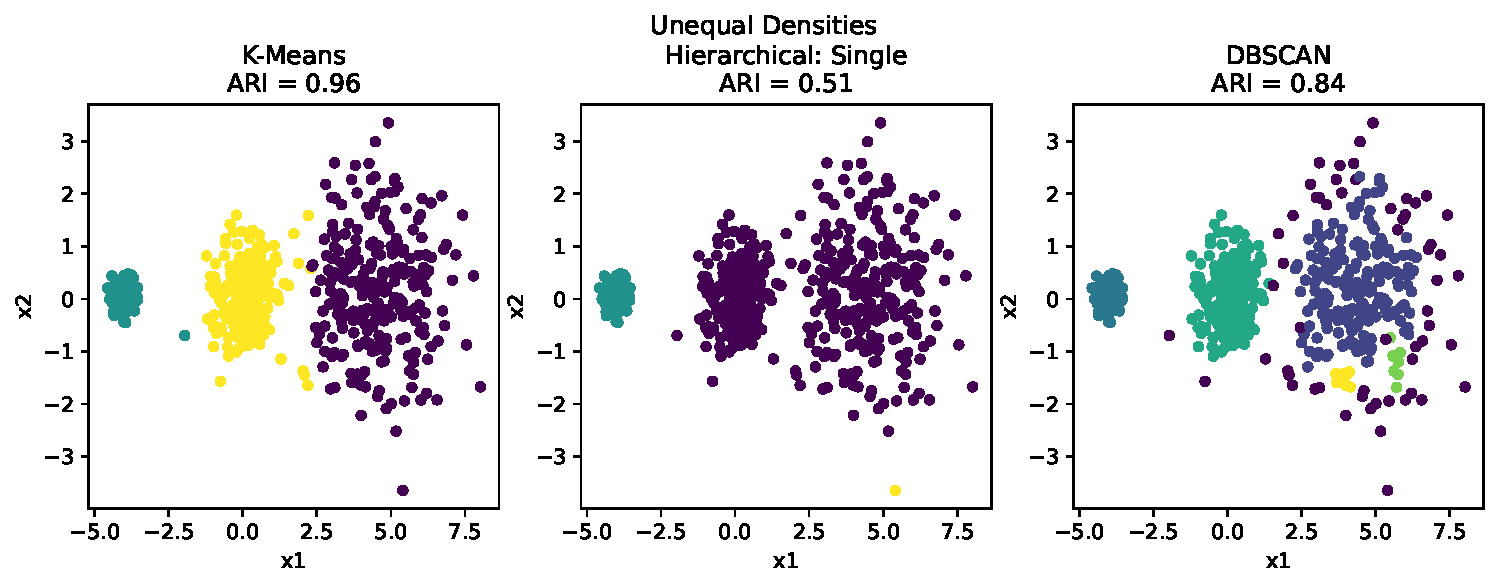
\includegraphics[keepaspectratio]{contents/3/cluster_files/figure-pdf/cell-27-output-1.pdf}}

The unequal-density dataset illustrates a limitation of DBSCAN. The
three groups have very different spreads.

\begin{itemize}
\tightlist
\item
  K-means is relatively effective here because the groups are still
  roughly center-based, even though their densities differ.
\item
  DBSCAN is less effective here than K-means and is more sensitive to
  the chosen \texttt{eps}, because one global \texttt{eps} may be
  appropriate for the dense group but too small for the sparse group, or
  appropriate for the sparse group but too large for the dense group.
\item
  Hierarchical clustering using single linkage can also be unstable here
  because a few close points between groups can create early connections
  that affect the later merges.
\end{itemize}

\subsection{Example: Uneven Chains}\label{example-uneven-chains}

\begin{Shaded}
\begin{Highlighting}[]
\NormalTok{rng\_chain }\OperatorTok{=}\NormalTok{ np.random.default\_rng(}\DecValTok{9}\NormalTok{)}
\NormalTok{t\_chain }\OperatorTok{=}\NormalTok{ np.concatenate([np.linspace(}\DecValTok{0}\NormalTok{, }\FloatTok{1.1}\NormalTok{, }\DecValTok{170}\NormalTok{), np.linspace(}\FloatTok{1.1}\NormalTok{, np.pi, }\DecValTok{35}\NormalTok{)])}
\NormalTok{upper\_chain }\OperatorTok{=}\NormalTok{ np.column\_stack([np.cos(t\_chain), np.sin(t\_chain)])}
\NormalTok{lower\_chain }\OperatorTok{=}\NormalTok{ np.column\_stack([}\DecValTok{1} \OperatorTok{{-}}\NormalTok{ np.cos(t\_chain), }\FloatTok{0.5} \OperatorTok{{-}}\NormalTok{ np.sin(t\_chain)])}
\NormalTok{X\_chain }\OperatorTok{=}\NormalTok{ np.vstack([upper\_chain, lower\_chain]) }\OperatorTok{+}\NormalTok{ rng\_chain.normal(}
\NormalTok{    scale}\OperatorTok{=}\FloatTok{0.025}\NormalTok{, size}\OperatorTok{=}\NormalTok{(}\DecValTok{2} \OperatorTok{*} \BuiltInTok{len}\NormalTok{(t\_chain), }\DecValTok{2}\NormalTok{)}
\NormalTok{)}
\NormalTok{true\_chain\_group }\OperatorTok{=}\NormalTok{ np.concatenate(}
\NormalTok{    [np.repeat(}\DecValTok{0}\NormalTok{, }\BuiltInTok{len}\NormalTok{(t\_chain)), np.repeat(}\DecValTok{1}\NormalTok{, }\BuiltInTok{len}\NormalTok{(t\_chain))]}
\NormalTok{)}

\NormalTok{kmeans\_labels }\OperatorTok{=}\NormalTok{ KMeans(n\_clusters}\OperatorTok{=}\DecValTok{2}\NormalTok{, n\_init}\OperatorTok{=}\DecValTok{20}\NormalTok{, random\_state}\OperatorTok{=}\DecValTok{1}\NormalTok{).fit\_predict(X\_chain)}

\NormalTok{single\_labels }\OperatorTok{=}\NormalTok{ AgglomerativeClustering(n\_clusters}\OperatorTok{=}\DecValTok{2}\NormalTok{, linkage}\OperatorTok{=}\StringTok{"single"}\NormalTok{).fit\_predict(}
\NormalTok{    X\_chain}
\NormalTok{)}
\NormalTok{dbscan\_labels }\OperatorTok{=}\NormalTok{ DBSCAN(eps}\OperatorTok{=}\FloatTok{0.08}\NormalTok{, min\_samples}\OperatorTok{=}\DecValTok{6}\NormalTok{).fit\_predict(X\_chain)}

\NormalTok{kmeans\_ari }\OperatorTok{=}\NormalTok{ adjusted\_rand\_score(true\_chain\_group, kmeans\_labels)}
\NormalTok{single\_ari }\OperatorTok{=}\NormalTok{ adjusted\_rand\_score(true\_chain\_group, single\_labels)}
\NormalTok{dbscan\_ari }\OperatorTok{=}\NormalTok{ adjusted\_rand\_score(true\_chain\_group, dbscan\_labels)}

\NormalTok{fig, axs }\OperatorTok{=}\NormalTok{ plt.subplots(}\DecValTok{1}\NormalTok{, }\DecValTok{3}\NormalTok{, figsize}\OperatorTok{=}\NormalTok{(}\DecValTok{12}\NormalTok{, }\FloatTok{3.5}\NormalTok{), sharex}\OperatorTok{=}\VariableTok{False}\NormalTok{, sharey}\OperatorTok{=}\VariableTok{False}\NormalTok{)}

\NormalTok{axs[}\DecValTok{0}\NormalTok{].scatter(X\_chain[:, }\DecValTok{0}\NormalTok{], X\_chain[:, }\DecValTok{1}\NormalTok{], c}\OperatorTok{=}\NormalTok{kmeans\_labels, s}\OperatorTok{=}\DecValTok{16}\NormalTok{)}
\NormalTok{axs[}\DecValTok{0}\NormalTok{].set\_title(}\SpecialStringTok{f"K{-}Means}\CharTok{\textbackslash{}n}\SpecialStringTok{ARI = }\SpecialCharTok{\{}\NormalTok{kmeans\_ari}\SpecialCharTok{:.2f\}}\SpecialStringTok{"}\NormalTok{)}

\NormalTok{axs[}\DecValTok{1}\NormalTok{].scatter(X\_chain[:, }\DecValTok{0}\NormalTok{], X\_chain[:, }\DecValTok{1}\NormalTok{], c}\OperatorTok{=}\NormalTok{single\_labels, s}\OperatorTok{=}\DecValTok{16}\NormalTok{)}
\NormalTok{axs[}\DecValTok{1}\NormalTok{].set\_title(}\SpecialStringTok{f"Hierarchical: Single}\CharTok{\textbackslash{}n}\SpecialStringTok{ARI = }\SpecialCharTok{\{}\NormalTok{single\_ari}\SpecialCharTok{:.2f\}}\SpecialStringTok{"}\NormalTok{)}

\NormalTok{axs[}\DecValTok{2}\NormalTok{].scatter(X\_chain[:, }\DecValTok{0}\NormalTok{], X\_chain[:, }\DecValTok{1}\NormalTok{], c}\OperatorTok{=}\NormalTok{dbscan\_labels, s}\OperatorTok{=}\DecValTok{16}\NormalTok{)}
\NormalTok{axs[}\DecValTok{2}\NormalTok{].set\_title(}\SpecialStringTok{f"DBSCAN}\CharTok{\textbackslash{}n}\SpecialStringTok{ARI = }\SpecialCharTok{\{}\NormalTok{dbscan\_ari}\SpecialCharTok{:.2f\}}\SpecialStringTok{"}\NormalTok{)}

\ControlFlowTok{for}\NormalTok{ ax }\KeywordTok{in}\NormalTok{ axs:}
\NormalTok{    ax.set\_xlabel(}\StringTok{"x1"}\NormalTok{)}
\NormalTok{    ax.set\_ylabel(}\StringTok{"x2"}\NormalTok{)}

\NormalTok{fig.suptitle(}\StringTok{"Uneven Chains"}\NormalTok{, y}\OperatorTok{=}\FloatTok{1.05}\NormalTok{)}\OperatorTok{;}
\end{Highlighting}
\end{Shaded}

\pandocbounded{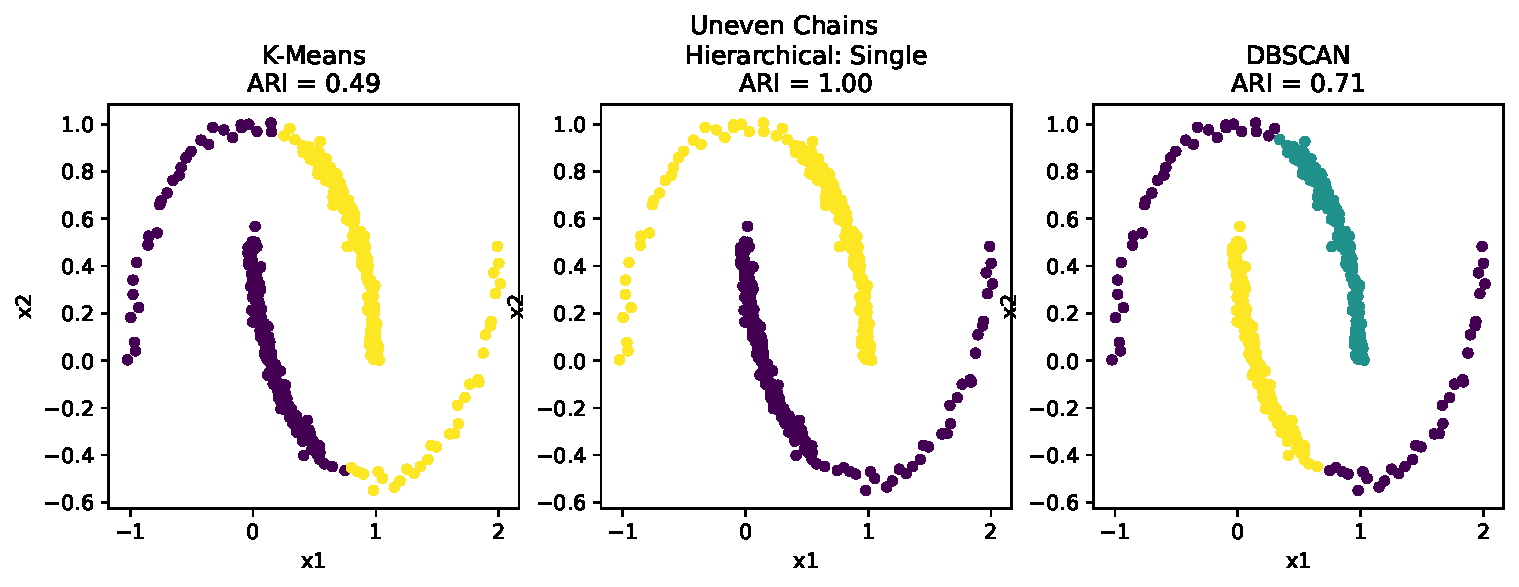
\includegraphics[keepaspectratio]{contents/3/cluster_files/figure-pdf/cell-28-output-1.pdf}}

The uneven-chain dataset illustrates a case where hierarchical
clustering using single linkage can be useful. The groups are best
described as connected chains with uneven spacing.

\begin{itemize}
\tightlist
\item
  Single linkage can follow each chain through nearest-neighbor
  connections, so it is the most natural fit among the three methods.
\item
  K-means instead cuts the plane into center-based regions, which mixes
  parts of the two chains.
\item
  DBSCAN can label the thinner parts on both sides of the chains as
  noise when one global density scale is used. In this example, those
  side segments are not merged into one cluster; they are mostly
  excluded as noise because they are too sparse under the chosen
  \texttt{eps} and \texttt{min\_samples}.
\end{itemize}

\chapter{Unsupervised Dimension Reduction}\label{sec-unsupervised-pca}

In the supervised dimension-reduction chapter, PCA appeared inside
principal component regression (PCR). There the workflow was

\[
X \longrightarrow Z=XV_m \longrightarrow \hat y.
\]

The principal components were useful only if they helped predict the
response. The number of components was therefore chosen by
cross-validation against prediction error.

This chapter uses the same algebra for a different purpose. There is no
response \(y\). The workflow is instead

\[
X \longrightarrow Z \longrightarrow \hat X.
\]

The question is no longer ``does the reduced representation predict
\(y\)?'' but ``what structure of the data matrix does the reduced
representation preserve?'' This change makes reconstruction,
compression, visualization, denoising, and distance preservation more
central than prediction.

We will use PCA as the main example, revisiting PCA, SVD, and related
concepts only where they help explain dimension reduction as a way of
building useful low-dimensional representations of a data matrix.

\section{How to Read the Data Matrix}\label{how-to-read-the-data-matrix}

Let \(X\in\mathbb R^{n\times p}\) contain \(n\) observations and \(p\)
features. We usually center the columns before applying PCA, so the
origin represents the sample mean.

This \(X\) has two complementary geometric views. The coordinates of a
vector determine the space it lives in. Therefore

\begin{itemize}
\tightlist
\item
  A row has one coordinate for each feature, so it is a vector in
  feature space \(\mathbb R^p\).
\item
  A column has one coordinate for each observation, so it is a vector in
  observation space \(\mathbb R^n\).
\end{itemize}

This is not only notation. It determines which objects can be compared,
combined, or projected. Row operations compare observations by their
feature values. Column operations compare features by their behavior
across observations.

\subsection{Rows: observations in feature
space}\label{rows-observations-in-feature-space}

The \(i\)-th row

\[
x_i^\top=\mqty[x_{i1},\ldots,x_{ip}]
\]

is one observation represented as a point in feature space
\(\mathbb R^p\). The axes of this space are the features. For example,
if the features are height, weight, and age, then each person is a point
in a three-dimensional feature space.

In this view, we ask questions about observations:

\begin{itemize}
\tightlist
\item
  Which observations are close to each other?
\item
  Which observations are outliers?
\item
  Can the observations be represented well by a lower-dimensional plane?
\end{itemize}

Distances between rows \(\norm{x_i-x_\ell}\) compare observations.
Clustering, nearest neighbors, and visualization usually start from this
row-side view. Dimension reduction replaces each high-dimensional row
\(x_i^\top\) with a lower-dimensional row \(z_i^\top\).

\subsection{Columns: features in observation
space}\label{columns-features-in-observation-space}

The \(j\)-th column

\[
X_j=\mqty[x_{1j},\ldots,x_{nj}]^\top
\]

is one feature measured across all observations. It is a vector in
observation space \(\mathbb R^n\). The axes of this space are the
individual observations. For example, the height column records the
height value for person 1, person 2, and so on. In that sense, height is
a point in an \(n\)-dimensional space whose coordinates are people.

In this view, we ask questions about features:

\begin{itemize}
\tightlist
\item
  Which features vary together across observations?
\item
  Which features are redundant?
\item
  Which weighted combinations of features create useful new features?
\end{itemize}

Inner products between columns \(X_j^\top X_k\) measure feature
co-movement. After centering, \(X_j^\top X_k/(n-1)\) is the sample
covariance between features \(j\) and \(k\). After standardizing
columns, the angle between \(X_j\) and \(X_k\) is related to their
correlation.

\subsection{A matrix is a bridge between two
spaces}\label{a-matrix-is-a-bridge-between-two-spaces}

Let \(e_i\in\mathbb R^n\) select observation \(i\), and let
\(f_j\in\mathbb R^p\) select feature \(j\). Then

\[
e_i^\top X f_j=x_{ij}.
\]

This single number connects the two spaces: it is the measurement of
feature \(j\) on observation \(i\). Reading across a row fixes an
observation and varies the feature index. Reading down a column fixes a
feature and varies the observation index.

More generally, \(X\) can combine many features or many observations at
once. If \(u\in\mathbb R^n\) and \(v\in\mathbb R^p\), then

\[
Xv\in\mathbb R^n,\qquad u^\top X\in\mathbb R^p,\qquad u^\top Xv\in\mathbb R.
\]

\begin{itemize}
\tightlist
\item
  The vector \(v\) gives weights for the features. Multiplying \(Xv\)
  makes one new feature column, with one value for each observation.
\item
  The vector \(u\) gives weights for the observations. Multiplying
  \(u^\top X\) makes one new row, with one value for each feature.
\end{itemize}

\begin{example}[Constructing a feature with
\(Xv\)]\protect\hypertarget{exm-feature-construction}{}\label{exm-feature-construction}

Suppose the rows of \(X\) are people and the columns are standardized
features such as height, weight, and age. To construct a new feature,
choose weights for the columns. For example, let

\[
v=
\mqty[0.6\\0.8\\0\\\vdots\\0],
\]

where the first two coordinates correspond to standardized height and
standardized weight. Then

\[
Xv=0.6X_1+0.8X_2.
\]

This is a new feature column in observation space \(\mathbb R^n\). Its
\(i\)-th entry is

\[
x_i^\top v=0.6x_{i1}+0.8x_{i2},
\]

a size-like score for person \(i\). The vector \(v\) is the recipe for
the new feature, and \(Xv\) lists that feature's values for all people.

\end{example}

\begin{example}[Aggregating observations with
\(u^\top X\)]\protect\hypertarget{exm-observation-aggregation}{}\label{exm-observation-aggregation}

Now mix rows instead of columns. The row \(x_i^\top\) contains all
feature values for person \(i\). If

\[
u=
\mqty[1/2\\1/2\\0\\\vdots\\0],
\]

then left-multiplying by \(u^\top\) gives

\[
u^\top X=\frac12x_1^\top+\frac12x_2^\top,
\]

the average values across all features for the first two people. This is
still a vector in feature space \(\mathbb R^p\): it has one coordinate
for height, one for weight, one for age, and so on.

If instead

\[
u=
\mqty[1/2\\-1/2\\0\\\vdots\\0],
\]

then

\[
u^\top X=\frac12x_1^\top-\frac12x_2^\top,
\]

which is a contrast between the first two people across all features.
Positive entries show features where person 1 is larger than person 2,
and negative entries show features where person 2 is larger than person
1.

\end{example}

\subsection{How to Interpret Principal Component
Vectors}\label{how-to-interpret-principal-component-vectors}

To interpret the principal component vectors, start from the singular
value decomposition of the centered data matrix
\(X\in\mathbb R^{n\times p}\). If \(\operatorname{rank}(X)=r\), then

\[
X=UDV^\top,\qquad Z=XV=UD,
\] where

\begin{itemize}
\tightlist
\item
  \(U\in\mathbb R^{n\times r}\) and \(V\in\mathbb R^{p\times r}\) have
  orthonormal columns;
\item
  \(D=\operatorname{diag}(d_1,\ldots,d_r)\) contains the positive
  singular values in decreasing order.
\end{itemize}

The columns of \(V\) are the principal component directions in feature
space. For component \(j\),

\[
v_j\in\mathbb R^p,\qquad Z_j=Xv_j\in\mathbb R^n.
\]

This is exactly the operation \(Xv\) discussed above: PCA chooses a
special feature-space direction \(v_j\) and uses \(Xv_j\) to combine the
original feature columns into one new score column.

The vector \(v_j\) is the loading vector. It gives the weights used to
combine the original feature columns:

\[
Z_j
=
v_{1j}X_1+\cdots+v_{pj}X_p.
\]

The vector \(Z_j\) is the score vector. It records the value of this new
component feature for every observation:

\[
z_{ij}=x_i^\top v_j.
\]

Equivalently, since \(Z=UD\), we have \(Z_j=d_ju_j\). The column \(u_j\)
gives the normalized score direction in observation space, while the
singular value \(d_j\) gives its scale.

\begin{example}[Reading loading signs and
magnitudes]\protect\hypertarget{exm-loading-signs}{}\label{exm-loading-signs}

Suppose one component uses two standardized features:

\[
z_{i1}=0.7x_{i1}+0.6x_{i2}.
\]

The two loadings have similar magnitude and the same sign. Both features
therefore contribute strongly, and both push the score in the same
direction: increasing either feature increases \(z_{i1}\), holding the
other feature fixed. Observations score high when both features are
high, and low when both features are low.

Now compare this with

\[
z_{i1}=0.7x_{i1}-0.6x_{i2}.
\]

The magnitudes are still similar, so both features matter. But the signs
are opposite: the first feature increases the score, while the second
decreases it. Observations score high when \(x_{i1}\) is large relative
to \(x_{i2}\), and low when \(x_{i2}\) is large relative to \(x_{i1}\).
The component is a contrast between the two features.

A feature with a near-zero loading would contribute little to this
component. The overall sign is arbitrary: multiplying both the loading
vector and the score vector by \(-1\) gives the same component.
Therefore, signs should be read relative to each other within the same
component.

\end{example}

Thus a principal component vector is not just a list of coefficients. It
is a direction in feature space, and its entries tell us how to combine
the original features to form a new score column. Entries with the same
sign capture shared variation among features, while entries with
opposite signs define a contrast between features.

\begin{definition}[Explained
variance]\protect\hypertarget{def-explained-variance}{}\label{def-explained-variance}

For centered data, the variance explained by component \(j\) is

\[
\lambda_j=\operatorname{Var}(Z_j)=\frac{d_j^2}{n-1}.
\]

The explained variance ratio of component \(j\) is

\[
\frac{\lambda_j}{\lambda_1+\cdots+\lambda_r}
=
\frac{d_j^2}{d_1^2+\cdots+d_r^2}.
\]

The cumulative explained variance ratio for the first \(m\) components
is

\[
\frac{\sum_{j=1}^m d_j^2}{\sum_{j=1}^r d_j^2}.
\]

\end{definition}

\subsection{PCA in Python}\label{pca-in-python}

As mentioned in PCR section, PCA is implemented by
\texttt{sklearn.decomposition.PCA}. The mathematical objects introduced
above correspond to the attributes and methods of a fitted
\texttt{PCA(n\_components=m)} object as follows:

{\def\LTcaptype{none} % do not increment counter
\begin{longtable}[]{@{}
  >{\raggedright\arraybackslash}p{(\linewidth - 2\tabcolsep) * \real{0.5000}}
  >{\raggedright\arraybackslash}p{(\linewidth - 2\tabcolsep) * \real{0.5000}}@{}}
\toprule\noalign{}
\begin{minipage}[b]{\linewidth}\raggedright
Mathematical object
\end{minipage} & \begin{minipage}[b]{\linewidth}\raggedright
\texttt{sklearn} attribute or method
\end{minipage} \\
\midrule\noalign{}
\endhead
\bottomrule\noalign{}
\endlastfoot
\(V_m^\top\in\mathbb R^{m\times p}\) & \texttt{pca.components\_} \\
\((d_1,\ldots,d_m)\) & \texttt{pca.singular\_values\_} \\
\(d_j^2/(n-1)\) & \texttt{pca.explained\_variance\_} \\
\(\dfrac{d_j^2}{\sum_{k=1}^r d_k^2}\) &
\texttt{pca.explained\_variance\_ratio\_} \\
\(Z_m=X_cV_m=U_mD_m\) & \texttt{pca.transform(X)} \\
\end{longtable}
}

In particular, each row of \texttt{pca.components\_} is one loading
vector \(v_j^\top\). Thus \texttt{pca.components\_} corresponds to
\(V_m^\top\), while \texttt{pca.components\_.T} corresponds to \(V_m\).

\begin{tcolorbox}[enhanced jigsaw, arc=.35mm, bottomrule=.15mm, bottomtitle=1mm, breakable, colback=white, colbacktitle=quarto-callout-note-color!10!white, colframe=quarto-callout-note-color-frame, coltitle=black, left=2mm, leftrule=.75mm, opacityback=0, opacitybacktitle=0.6, rightrule=.15mm, title=\textcolor{quarto-callout-note-color}{\faInfo}\hspace{0.5em}{Centering notation}, titlerule=0mm, toprule=.15mm, toptitle=1mm]

\texttt{sklearn} accepts a raw data matrix \(X\) and centers it
internally. Let \(\mu\) be the column-wise mean of \(X\) and let
\(X_c=X-\mu\). Then \texttt{pca.mean\_} stores \(\mu\), and the SVD
underlying PCA is applied to the centered matrix \(X_c=UDV^\top\).
Therefore, \texttt{pca.transform(X)} gives \(X_cV_m=U_mD_m\).

In other words, to reconstruct the original \(X\) (as discussed in the
following sections), you need to add \(\mu\) back afterward.

\end{tcolorbox}

\section{PCA as Reconstruction}\label{pca-as-reconstruction}

With loadings and scores in place, PCA can be read as a reconstruction
method. Assume \(X\) is centered and has rank \(r\). Its singular value
decomposition is

\[
X=UDV^\top
=
d_1u_1v_1^\top+\cdots+d_ru_rv_r^\top,
\]

where \(d_1\ge\cdots\ge d_r>0\). Keeping only the first \(m\) terms
gives

\[
\hat X_m
=
U_mD_mV_m^\top
=
Z_mV_m^\top,
\qquad
Z_m=XV_m=U_mD_m.
\]

This is the rank-\(m\) PCA reconstruction of \(X\). It first builds
\(m\) new derived features,

\[
Z_m=(Xv_1,\ldots,Xv_m),
\]

then maps those \(m\) score columns back to the original feature space.
In this sense, PCA compression replaces the original \(p\) features by
\(m\) carefully chosen feature combinations.

The important optimality result is:

\[
\hat X_m
=
\operatorname*{argmin}_{A\in\mathbb R^{n\times p},\ \operatorname{rank}(A)\le m}
\norm{X-A}_F^2.
\]

Here \(A\) is any candidate rank-\(m\) approximation to \(X\), and
\(\norm{\cdot}_F\) is the Frobenius norm:

\[
\norm{X-A}_F^2
=
\sum_{i=1}^n\sum_{j=1}^p (x_{ij}-a_{ij})^2.
\]

Then the reconstruction error is

\[
\norm{X-\hat X_m}_F^2
=
\sum_{j=m+1}^r d_j^2.
\]

This is the unsupervised meaning of PCA: among all \(m\)-dimensional
linear representations, PCA gives the best squared-error reconstruction
of the centered data matrix.

\begin{tcolorbox}[enhanced jigsaw, arc=.35mm, bottomrule=.15mm, bottomtitle=1mm, breakable, colback=white, colbacktitle=quarto-callout-important-color!10!white, colframe=quarto-callout-important-color-frame, coltitle=black, left=2mm, leftrule=.75mm, opacityback=0, opacitybacktitle=0.6, rightrule=.15mm, title=\textcolor{quarto-callout-important-color}{\faExclamation}\hspace{0.5em}{PCA optimizes reconstruction, not every downstream task}, titlerule=0mm, toprule=.15mm, toptitle=1mm]

PCA preserves directions with large variance because those directions
minimize squared reconstruction error. This does not guarantee that the
leading components preserve class separation, rare groups, causal
structure, or predictive signal.

If we use the PCA scores as predictors in a linear regression, we obtain
principal component regression (PCR). PCR adds a supervised prediction
step, and the number of retained components may be selected using \(y\),
but the PCA directions themselves are still chosen without using \(y\).

\end{tcolorbox}

\subsection{A Two-Dimensional Reconstruction
Example}\label{a-two-dimensional-reconstruction-example}

The dataset is generated in the following way. To make the later PCA
workflow simpler, we center the data from the beginning.

\protect\phantomsection\label{annotated-cell-260}%
\begin{Shaded}
\begin{Highlighting}[]
\ImportTok{import}\NormalTok{ numpy }\ImportTok{as}\NormalTok{ np}

\NormalTok{rng }\OperatorTok{=}\NormalTok{ np.random.default\_rng(}\DecValTok{1}\NormalTok{)}

\NormalTok{Sigma }\OperatorTok{=}\NormalTok{ np.array([}
\NormalTok{        [}\FloatTok{0.5}\NormalTok{, }\OperatorTok{{-}}\FloatTok{0.65}\NormalTok{],}
\NormalTok{        [}\OperatorTok{{-}}\FloatTok{0.65}\NormalTok{, }\FloatTok{1.0}\NormalTok{],}
\NormalTok{    ])}

\NormalTok{X\_original }\OperatorTok{=}\NormalTok{ rng.multivariate\_normal(mean}\OperatorTok{=}\NormalTok{[}\DecValTok{1}\NormalTok{, }\DecValTok{2}\NormalTok{], cov}\OperatorTok{=}\NormalTok{Sigma, size}\OperatorTok{=}\DecValTok{100}\NormalTok{)}
\NormalTok{X\_centered }\OperatorTok{=}\NormalTok{ X\_original }\OperatorTok{{-}}\NormalTok{ X\_original.mean(axis}\OperatorTok{=}\DecValTok{0}\NormalTok{) }\CommentTok{\# \textless{}1\textgreater{}}
\end{Highlighting}
\end{Shaded}

\begin{description}
\tightlist
\item[5CB6E08D-list-annote-1]
\texttt{StandardScaler(with\_std=False)} also works.
\end{description}

We perform PCA and inverse-transform the one-dimensional scores to
reconstruct the data in the original feature space.

\begin{Shaded}
\begin{Highlighting}[]
\ImportTok{from}\NormalTok{ sklearn.decomposition }\ImportTok{import}\NormalTok{ PCA}
\ImportTok{import}\NormalTok{ matplotlib.pyplot }\ImportTok{as}\NormalTok{ plt}

\NormalTok{pca\_1d }\OperatorTok{=}\NormalTok{ PCA(n\_components}\OperatorTok{=}\DecValTok{1}\NormalTok{)}
\NormalTok{score\_1d }\OperatorTok{=}\NormalTok{ pca\_1d.fit\_transform(X\_centered)}
\NormalTok{X\_hat\_1d }\OperatorTok{=}\NormalTok{ pca\_1d.inverse\_transform(score\_1d)}

\NormalTok{plt.scatter(X\_centered[:, }\DecValTok{0}\NormalTok{], X\_centered[:, }\DecValTok{1}\NormalTok{], label}\OperatorTok{=}\StringTok{"data"}\NormalTok{)}
\NormalTok{plt.scatter(X\_hat\_1d[:, }\DecValTok{0}\NormalTok{], X\_hat\_1d[:, }\DecValTok{1}\NormalTok{], label}\OperatorTok{=}\StringTok{"rank{-}1 reconstruction"}\NormalTok{)}

\NormalTok{plt.xlabel(}\StringTok{"x1"}\NormalTok{)}
\NormalTok{plt.ylabel(}\StringTok{"x2"}\NormalTok{)}
\NormalTok{plt.title(}\StringTok{"PCA Projection and Reconstruction"}\NormalTok{)}
\NormalTok{plt.legend()}\OperatorTok{;}
\end{Highlighting}
\end{Shaded}

\pandocbounded{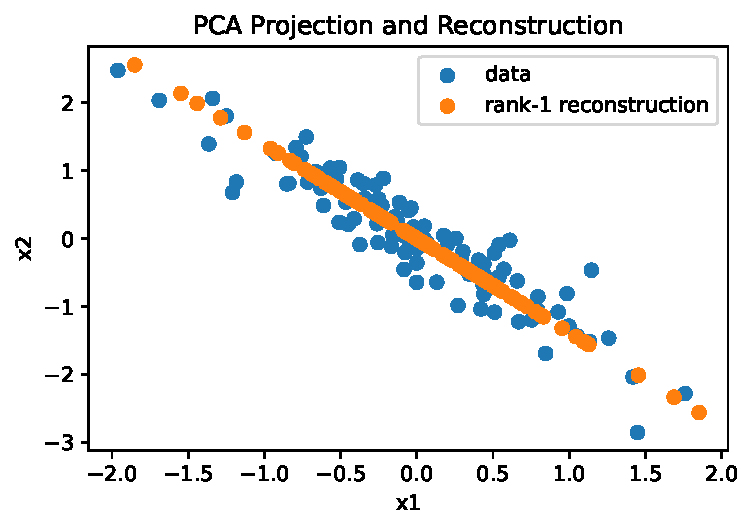
\includegraphics[keepaspectratio]{contents/3/dimensionr_files/figure-pdf/cell-3-output-1.pdf}}

The orange points are not new observations. They are the rank-1
reconstructions of the original observations obtained by projecting the
data onto the first principal component and then mapping them back to
the original space. Under the squared-error criterion, this gives the
best rank-1 approximation.

\subsection{Centering, Scaling, and What PCA
Preserves}\label{centering-scaling-and-what-pca-preserves}

PCA depends on the geometry of the input matrix.

Centering is usually essential. Without centering, the first principal
component may partly reflect the location of the data cloud relative to
the origin rather than the variation around the mean. This is the same
phenomenon illustrated in Example~\ref{exm-centering_and_scaling}.

Scaling is a modeling choice. \texttt{sklearn.decomposition.PCA} centers
features automatically, but it does not scale them to unit variance.
Because the loading vector assigns weights to the input variables,
variables with larger scales contribute more to the covariance matrix
and therefore tend to have greater influence on the principal
components. In practice, the following guidelines are commonly used:

\begin{itemize}
\tightlist
\item
  Scale the variables when their units are not comparable.
\item
  Do not scale them when the original magnitude of variation is
  meaningful.
\item
  State the choice explicitly, because it changes the covariance matrix
  and therefore the principal components.
\end{itemize}

\begin{example}[]\protect\hypertarget{exm-}{}\label{exm-}

We first create a version of the same data in which \texttt{x2} is
measured on a scale ten times larger than \texttt{x1}.

\begin{Shaded}
\begin{Highlighting}[]
\NormalTok{X\_modified }\OperatorTok{=}\NormalTok{ X\_original }\OperatorTok{*}\NormalTok{ np.array([}\DecValTok{1}\NormalTok{, }\DecValTok{10}\NormalTok{])}
\end{Highlighting}
\end{Shaded}

Now compare PCA with and without standardization.

\begin{Shaded}
\begin{Highlighting}[]
\ImportTok{from}\NormalTok{ sklearn.preprocessing }\ImportTok{import}\NormalTok{ StandardScaler}
\ImportTok{from}\NormalTok{ sklearn.decomposition }\ImportTok{import}\NormalTok{ PCA}
\ImportTok{import}\NormalTok{ pandas }\ImportTok{as}\NormalTok{ pd}

\NormalTok{X\_scaled }\OperatorTok{=}\NormalTok{ StandardScaler().fit\_transform(X\_modified)}

\NormalTok{pca\_centered }\OperatorTok{=}\NormalTok{ PCA(n\_components}\OperatorTok{=}\DecValTok{2}\NormalTok{).fit(X\_modified)}
\NormalTok{pca\_scaled }\OperatorTok{=}\NormalTok{ PCA(n\_components}\OperatorTok{=}\DecValTok{2}\NormalTok{).fit(X\_scaled)}

\NormalTok{pd.DataFrame(}
\NormalTok{    \{}
        \StringTok{"centered only"}\NormalTok{: pca\_centered.explained\_variance\_ratio\_,}
        \StringTok{"centered and scaled"}\NormalTok{: pca\_scaled.explained\_variance\_ratio\_,}
\NormalTok{    \},}
\NormalTok{    index}\OperatorTok{=}\NormalTok{[}\StringTok{"PC1"}\NormalTok{, }\StringTok{"PC2"}\NormalTok{],}
\NormalTok{)}
\end{Highlighting}
\end{Shaded}

{\def\LTcaptype{none} % do not increment counter
\begin{longtable}[]{@{}lll@{}}
\toprule\noalign{}
& centered only & centered and scaled \\
\midrule\noalign{}
\endhead
\bottomrule\noalign{}
\endlastfoot
PC1 & 0.999259 & 0.964569 \\
PC2 & 0.000741 & 0.035431 \\
\end{longtable}
}

The two analyses use the same observations, but the second feature has
been measured on a scale ten times larger. Without scaling, PCA treats
that larger numerical variation as geometrically important, and
therefore PC1 dominates. After standardizing, the comparison is based on
the correlation structure instead of the raw units. PC2 can then explain
a nontrivial share of the standardized variance, because PCA is no
longer dominated by the raw numerical scale of the second feature.

\end{example}

\begin{tcolorbox}[enhanced jigsaw, arc=.35mm, bottomrule=.15mm, bottomtitle=1mm, breakable, colback=white, colbacktitle=quarto-callout-caution-color!10!white, colframe=quarto-callout-caution-color-frame, coltitle=black, left=2mm, leftrule=.75mm, opacityback=0, opacitybacktitle=0.6, rightrule=.15mm, title=\textcolor{quarto-callout-caution-color}{\faFire}\hspace{0.5em}{Preprocessing defines the geometry}, titlerule=0mm, toprule=.15mm, toptitle=1mm]

PCA does not know which units are scientifically meaningful. Changing
units, transforming variables, or standardizing features changes the
geometry that PCA tries to preserve.

\end{tcolorbox}

\subsection{\texorpdfstring{Choosing a Dimension Without
\(y\)}{Choosing a Dimension Without y}}\label{choosing-a-dimension-without-y}

In PCR, the number of components is chosen by prediction error. Without
\(y\), the choice must be tied to the representation goal.

Common criteria include:

\begin{itemize}
\tightlist
\item
  cumulative explained variance;
\item
  reconstruction error;
\item
  visual interpretability in two or three dimensions;
\item
  denoising performance;
\item
  stability of a downstream unsupervised method such as clustering;
\item
  computational constraints.
\end{itemize}

The right criterion depends on the goal of the analysis. As one common
example, we can choose \(m\) by setting a threshold for the cumulative
explained variance ratio.

\begin{example}[]\protect\hypertarget{exm-}{}\label{exm-}

We use the digits dataset from \texttt{sklearn} to demonstrate the
example. This is about handwritten digits. The
\href{https://scikit-learn.org/stable/modules/generated/sklearn.datasets.load_digits.html}{dataset}
is from \texttt{sklearn} that is partially copied from
\href{https://archive.ics.uci.edu/dataset/80/optical+recognition+of+handwritten+digits}{UCI
machine learning repository}.

The dataset contains 1797 8x8 images. The data flattens the images into
1D arrays, and therefore the dataset is a \texttt{(1797,\ 64)} numpy
array.

\begin{Shaded}
\begin{Highlighting}[]
\ImportTok{from}\NormalTok{ sklearn.datasets }\ImportTok{import}\NormalTok{ load\_digits}

\NormalTok{X\_digits }\OperatorTok{=}\NormalTok{ load\_digits().data}
\end{Highlighting}
\end{Shaded}

We use \texttt{np.cumsum()} to find the total variance explained of the
first several components. In this example, we decide to use
\texttt{90\%} as the threshold to determine the number of components.
This 90\% threshold is only for illustration; there is no special reason
that this example must use 90\%.

\begin{Shaded}
\begin{Highlighting}[]
\NormalTok{digits\_pca\_full }\OperatorTok{=}\NormalTok{ PCA().fit(X\_digits)}
\NormalTok{cum\_ratio }\OperatorTok{=}\NormalTok{ np.cumsum(digits\_pca\_full.explained\_variance\_ratio\_)}

\NormalTok{fig, ax }\OperatorTok{=}\NormalTok{ plt.subplots(figsize}\OperatorTok{=}\NormalTok{(}\DecValTok{7}\NormalTok{, }\DecValTok{4}\NormalTok{))}
\NormalTok{ax.plot(np.arange(}\DecValTok{1}\NormalTok{, }\BuiltInTok{len}\NormalTok{(cum\_ratio) }\OperatorTok{+} \DecValTok{1}\NormalTok{), cum\_ratio, marker}\OperatorTok{=}\StringTok{\textquotesingle{}o\textquotesingle{}}\NormalTok{)}
\NormalTok{ax.axhline(}\FloatTok{0.90}\NormalTok{, color}\OperatorTok{=}\StringTok{"C1"}\NormalTok{, linestyle}\OperatorTok{=}\StringTok{"{-}{-}"}\NormalTok{, label}\OperatorTok{=}\StringTok{"90\%"}\NormalTok{)}
\NormalTok{ax.set\_xlabel(}\StringTok{"number of components"}\NormalTok{)}
\NormalTok{ax.set\_ylabel(}\StringTok{"cumulative explained variance"}\NormalTok{)}
\NormalTok{ax.set\_title(}\StringTok{"Digits: Cumulative Explained Variance"}\NormalTok{)}
\NormalTok{ax.legend()}\OperatorTok{;}
\end{Highlighting}
\end{Shaded}

\pandocbounded{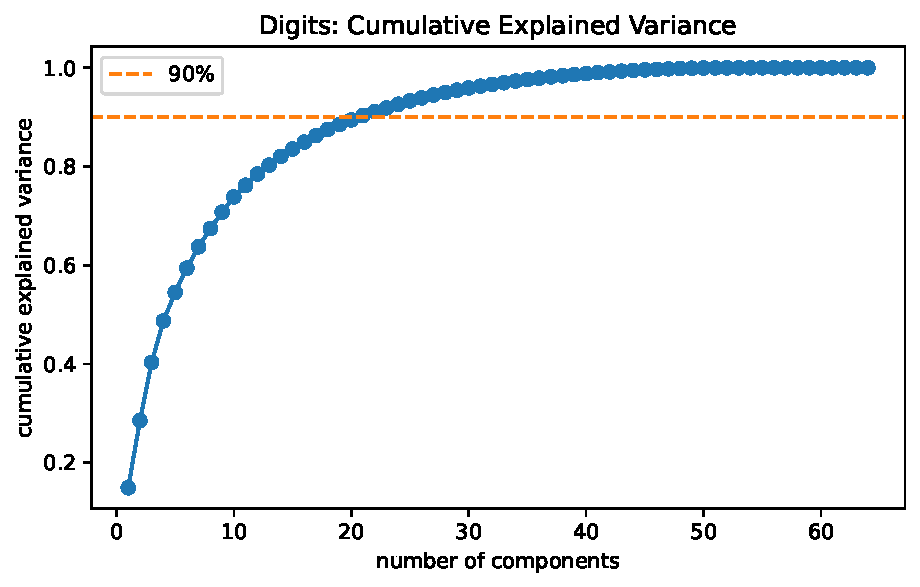
\includegraphics[keepaspectratio]{contents/3/dimensionr_files/figure-pdf/cell-7-output-1.pdf}}

If it is not easy to read from the plot, we can also use
\texttt{np.argmax} to find the first term that \texttt{cum\_ratio}
exceeds \texttt{.90}.

\protect\phantomsection\label{annotated-cell-506}%
\begin{Shaded}
\begin{Highlighting}[]
\NormalTok{np.argmax(cum\_ratio }\OperatorTok{\textgreater{}=} \FloatTok{0.90}\NormalTok{) }\OperatorTok{+} \DecValTok{1} \CommentTok{\# \textless{}1\textgreater{}}
\end{Highlighting}
\end{Shaded}

\begin{description}
\tightlist
\item[5CB6E08D-list-annote-1]
\texttt{np.argmax(cum\_ratio\ \textgreater{}=\ 0.90)} returns the first
0-based index where the cumulative ratio reaches 0.90. The \texttt{+1}
converts that index to the number of components.
\end{description}

\begin{verbatim}
np.int64(21)
\end{verbatim}

This number answers a reconstruction-style question: how many components
are needed to explain 90\% of the sample variance? It does not
automatically answer how many components are best for clustering,
classification, or scientific interpretation.

\end{example}

\begin{tcolorbox}[enhanced jigsaw, arc=.35mm, bottomrule=.15mm, bottomtitle=1mm, breakable, colback=white, colbacktitle=quarto-callout-note-color!10!white, colframe=quarto-callout-note-color-frame, coltitle=black, left=2mm, leftrule=.75mm, opacityback=0, opacitybacktitle=0.6, rightrule=.15mm, title=\textcolor{quarto-callout-note-color}{\faInfo}\hspace{0.5em}{Choosing an explained-variance threshold}, titlerule=0mm, toprule=.15mm, toptitle=1mm]

In practice, the threshold should be justified for the specific goal of
the analysis. There is no universal threshold that works for all PCA
applications.

Common values such as 90\%, 95\%, or 99\% are heuristics for
reconstruction or compression. A higher threshold keeps more detail but
gives less dimension reduction; a lower threshold gives stronger
compression but may lose important structure.

For visualization, we usually choose 2 or 3 components directly. For
denoising, an elbow in the scree plot or visible reconstruction quality
may be more useful than a fixed percentage. For clustering or other
downstream unsupervised tasks, try several values of \(m\) and check
whether the downstream result is stable.

\end{tcolorbox}

\section{More Applications of PCA}\label{more-applications-of-pca}

Different goals lead to different choices of \(m\). We now look at three
common uses of PCA: compression, denoising, and preprocessing.

\subsection{Compression}\label{compression}

Low-rank reconstruction can compress data by storing the scores \(Z_m\)
and loadings \(V_m\) instead of all of \(X\). The scores are the values
of \(m\) derived features; the loadings say how those derived features
relate back to the original \(p\) features.

There are two storage costs: shared quantities, such as the loading
matrix and feature means, and per-observation quantities, namely the
\(m\) scores. PCA compression is therefore most useful when many
observations share the same fitted PCA basis.

For images, reconstruction makes the compression tradeoff visible.

We use the digits dataset introduced above to illustrate the idea.

\begin{Shaded}
\begin{Highlighting}[]
\ImportTok{from}\NormalTok{ sklearn.datasets }\ImportTok{import}\NormalTok{ load\_digits}

\NormalTok{X\_digits }\OperatorTok{=}\NormalTok{ load\_digits().data}
\end{Highlighting}
\end{Shaded}

We fit PCA on the full digits dataset, and then visualize the
reconstruction of the image at index 0.

\begin{Shaded}
\begin{Highlighting}[]
\NormalTok{x0 }\OperatorTok{=}\NormalTok{ X\_digits[[}\DecValTok{0}\NormalTok{]]}
\end{Highlighting}
\end{Shaded}

Once the flattened array is reshaped into an \texttt{8x8} matrix, we may
use \texttt{imshow()} to display the image. We then apply \texttt{PCA}
and display the reconstructed images.

\begin{Shaded}
\begin{Highlighting}[]
\ImportTok{from}\NormalTok{ sklearn.decomposition }\ImportTok{import}\NormalTok{ PCA}

\NormalTok{components\_to\_show }\OperatorTok{=}\NormalTok{ [}\DecValTok{2}\NormalTok{, }\DecValTok{8}\NormalTok{, }\DecValTok{16}\NormalTok{, }\DecValTok{32}\NormalTok{]}

\NormalTok{fig, axs }\OperatorTok{=}\NormalTok{ plt.subplots(}\DecValTok{1}\NormalTok{, }\BuiltInTok{len}\NormalTok{(components\_to\_show) }\OperatorTok{+} \DecValTok{1}\NormalTok{, figsize}\OperatorTok{=}\NormalTok{(}\DecValTok{11}\NormalTok{, }\FloatTok{2.3}\NormalTok{))}

\NormalTok{axs[}\DecValTok{0}\NormalTok{].imshow(x0.reshape(}\DecValTok{8}\NormalTok{, }\DecValTok{8}\NormalTok{), cmap}\OperatorTok{=}\StringTok{"gray\_r"}\NormalTok{)}
\NormalTok{axs[}\DecValTok{0}\NormalTok{].set\_title(}\StringTok{"Original"}\NormalTok{)}
\NormalTok{axs[}\DecValTok{0}\NormalTok{].axis(}\StringTok{"off"}\NormalTok{)}

\ControlFlowTok{for}\NormalTok{ ax, m }\KeywordTok{in} \BuiltInTok{zip}\NormalTok{(axs[}\DecValTok{1}\NormalTok{:], components\_to\_show):}
\NormalTok{    pca\_m }\OperatorTok{=}\NormalTok{ PCA(n\_components}\OperatorTok{=}\NormalTok{m).fit(X\_digits)}
\NormalTok{    x\_hat }\OperatorTok{=}\NormalTok{ pca\_m.inverse\_transform(pca\_m.transform(x0))}
\NormalTok{    ax.imshow(x\_hat.reshape(}\DecValTok{8}\NormalTok{, }\DecValTok{8}\NormalTok{), cmap}\OperatorTok{=}\StringTok{"gray\_r"}\NormalTok{)}
\NormalTok{    ax.set\_title(}\SpecialStringTok{f"}\SpecialCharTok{\{}\NormalTok{m}\SpecialCharTok{\}}\SpecialStringTok{ PCs"}\NormalTok{)}
\NormalTok{    ax.axis(}\StringTok{"off"}\NormalTok{)}\OperatorTok{;}
\end{Highlighting}
\end{Shaded}

\pandocbounded{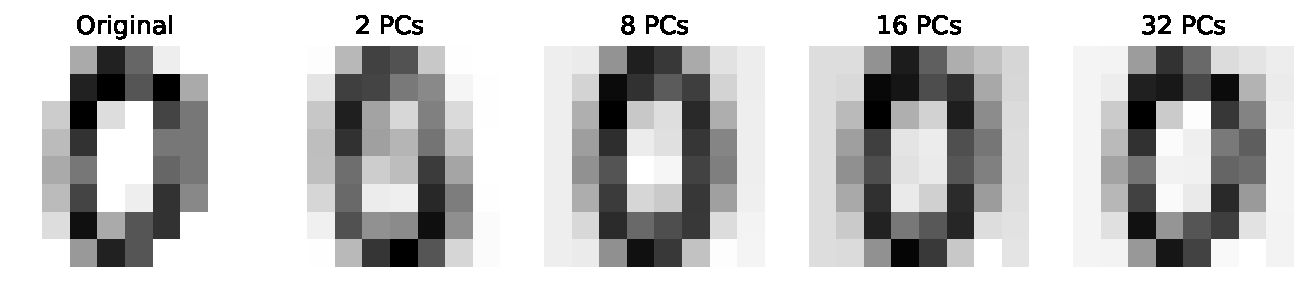
\includegraphics[keepaspectratio]{contents/3/dimensionr_files/figure-pdf/cell-11-output-1.pdf}}

Small \(m\) produces a rough reconstruction because many components have
been discarded. Larger \(m\) restores more detail, but it also requires
storing more scores and loadings. Because this digit is relatively
simple, the visual differences between some reconstructions may be
subtle.

We can measure the per-image storage after the PCA loading matrix has
been learned and shared across the dataset. Each original image stores
64 pixel values. With \(m\) components, each image is represented by
\(m\) scores. Ignoring the shared loading matrix and feature means, the
theoretical per-image storage ratios are:

{\def\LTcaptype{none} % do not increment counter
\begin{longtable}[]{@{}llll@{}}
\toprule\noalign{}
& scores per image & original values per image & relative storage per
image \\
\midrule\noalign{}
\endhead
\bottomrule\noalign{}
\endlastfoot
2 PCs & 2 & 64 & 0.03125 \\
8 PCs & 8 & 64 & 0.12500 \\
16 PCs & 16 & 64 & 0.25000 \\
32 PCs & 32 & 64 & 0.50000 \\
\end{longtable}
}

We can also check the actual memory used by the NumPy arrays with
\texttt{.nbytes}. Since \texttt{sklearn.PCA} centers the data, the
compressed representation must store the scores, the loading matrix, and
the feature means needed for reconstruction.

\begin{Shaded}
\begin{Highlighting}[]
\NormalTok{original\_bytes }\OperatorTok{=}\NormalTok{ X\_digits.nbytes}

\NormalTok{storage\_rows }\OperatorTok{=}\NormalTok{ []}
\ControlFlowTok{for}\NormalTok{ m }\KeywordTok{in}\NormalTok{ components\_to\_show:}
\NormalTok{    pca\_m }\OperatorTok{=}\NormalTok{ PCA(n\_components}\OperatorTok{=}\NormalTok{m).fit(X\_digits)}
\NormalTok{    Z\_m }\OperatorTok{=}\NormalTok{ pca\_m.transform(X\_digits)}

\NormalTok{    compressed\_bytes }\OperatorTok{=}\NormalTok{ Z\_m.nbytes }\OperatorTok{+}\NormalTok{ pca\_m.components\_.nbytes }\OperatorTok{+}\NormalTok{ pca\_m.mean\_.nbytes}
\NormalTok{    storage\_rows.append(}
\NormalTok{        \{}
            \StringTok{"components"}\NormalTok{: m,}
            \StringTok{"original KB"}\NormalTok{: original\_bytes }\OperatorTok{/} \DecValTok{1024}\NormalTok{,}
            \StringTok{"compressed KB"}\NormalTok{: compressed\_bytes }\OperatorTok{/} \DecValTok{1024}\NormalTok{,}
            \StringTok{"compressed / original"}\NormalTok{: compressed\_bytes }\OperatorTok{/}\NormalTok{ original\_bytes,}
\NormalTok{        \}}
\NormalTok{    )}

\NormalTok{pd.DataFrame(storage\_rows)}
\end{Highlighting}
\end{Shaded}

{\def\LTcaptype{none} % do not increment counter
\begin{longtable}[]{@{}lllll@{}}
\toprule\noalign{}
& components & original KB & compressed KB & compressed / original \\
\midrule\noalign{}
\endhead
\bottomrule\noalign{}
\endlastfoot
0 & 2 & 898.5 & 29.578125 & 0.032919 \\
1 & 8 & 898.5 & 116.812500 & 0.130008 \\
2 & 16 & 898.5 & 233.125000 & 0.259460 \\
3 & 32 & 898.5 & 465.750000 & 0.518364 \\
\end{longtable}
}

These measured ratios are slightly larger because they include the
shared quantities, not only the score values for each image.

For a single image alone, PCA is not necessarily a compression method.
The benefit comes when many observations share the same loading matrix
and each observation only needs its own low-dimensional score vector.

\subsection{Denoising}\label{denoising}

PCA can also denoise data when noise is spread across many low-variance
directions and signal is concentrated in the leading components. In that
case, reconstructing with a moderate number of components can keep the
main structure while discarding some noise.

We illustrate the idea by adding noise to the \texttt{x0} image from the
digits dataset.

\begin{Shaded}
\begin{Highlighting}[]
\ImportTok{from}\NormalTok{ sklearn.datasets }\ImportTok{import}\NormalTok{ load\_digits}

\NormalTok{X\_digits }\OperatorTok{=}\NormalTok{ load\_digits().data}
\NormalTok{x0 }\OperatorTok{=}\NormalTok{ X\_digits[[}\DecValTok{0}\NormalTok{]]}

\NormalTok{rng }\OperatorTok{=}\NormalTok{ np.random.default\_rng(}\DecValTok{3}\NormalTok{)}
\NormalTok{x\_noisy }\OperatorTok{=}\NormalTok{ x0 }\OperatorTok{+}\NormalTok{ rng.normal(scale}\OperatorTok{=}\DecValTok{4}\NormalTok{, size}\OperatorTok{=}\NormalTok{x0.shape)}
\end{Highlighting}
\end{Shaded}

We learn the PCA basis from the full digits dataset, not from this
single noisy image. The leading directions therefore represent common
digit-shaped variation, while the added pixel noise is less aligned with
those directions.

For denoising, \(m\) is often chosen by inspecting reconstruction
quality or by looking for an elbow in the explained-variance curve,
rather than by using a fixed threshold. Here we use 16 components as an
illustrative middle ground: enough to preserve the main digit shape, but
not so many that the reconstruction simply keeps all of the noisy
variation.

\begin{Shaded}
\begin{Highlighting}[]
\ImportTok{from}\NormalTok{ sklearn.decomposition }\ImportTok{import}\NormalTok{ PCA}

\NormalTok{m\_denoise }\OperatorTok{=} \DecValTok{16}
\NormalTok{pca\_denoise }\OperatorTok{=}\NormalTok{ PCA(n\_components}\OperatorTok{=}\NormalTok{m\_denoise).fit(X\_digits)}
\NormalTok{x\_denoised }\OperatorTok{=}\NormalTok{ pca\_denoise.inverse\_transform(pca\_denoise.transform(x\_noisy))}
\end{Highlighting}
\end{Shaded}

\begin{Shaded}
\begin{Highlighting}[]
\ImportTok{import}\NormalTok{ matplotlib.pyplot }\ImportTok{as}\NormalTok{ plt}

\NormalTok{fig, axs }\OperatorTok{=}\NormalTok{ plt.subplots(}\DecValTok{1}\NormalTok{, }\DecValTok{3}\NormalTok{, figsize}\OperatorTok{=}\NormalTok{(}\FloatTok{7.5}\NormalTok{, }\FloatTok{2.5}\NormalTok{))}

\NormalTok{axs[}\DecValTok{0}\NormalTok{].imshow(x0.reshape(}\DecValTok{8}\NormalTok{, }\DecValTok{8}\NormalTok{), cmap}\OperatorTok{=}\StringTok{"gray\_r"}\NormalTok{)}
\NormalTok{axs[}\DecValTok{0}\NormalTok{].set\_title(}\StringTok{"Original"}\NormalTok{)}
\NormalTok{axs[}\DecValTok{0}\NormalTok{].axis(}\StringTok{"off"}\NormalTok{)}

\NormalTok{axs[}\DecValTok{1}\NormalTok{].imshow(x\_noisy.reshape(}\DecValTok{8}\NormalTok{, }\DecValTok{8}\NormalTok{), cmap}\OperatorTok{=}\StringTok{"gray\_r"}\NormalTok{)}
\NormalTok{axs[}\DecValTok{1}\NormalTok{].set\_title(}\StringTok{"Noisy"}\NormalTok{)}
\NormalTok{axs[}\DecValTok{1}\NormalTok{].axis(}\StringTok{"off"}\NormalTok{)}

\NormalTok{axs[}\DecValTok{2}\NormalTok{].imshow(x\_denoised.reshape(}\DecValTok{8}\NormalTok{, }\DecValTok{8}\NormalTok{), cmap}\OperatorTok{=}\StringTok{"gray\_r"}\NormalTok{)}
\NormalTok{axs[}\DecValTok{2}\NormalTok{].set\_title(}\StringTok{"Denoised"}\NormalTok{)}
\NormalTok{axs[}\DecValTok{2}\NormalTok{].axis(}\StringTok{"off"}\NormalTok{)}\OperatorTok{;}
\end{Highlighting}
\end{Shaded}

\pandocbounded{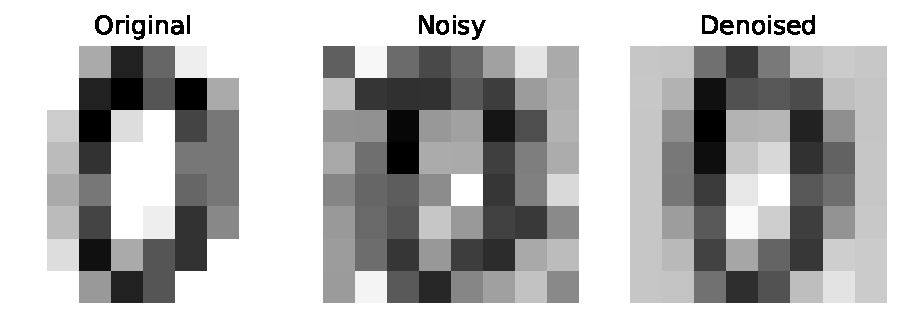
\includegraphics[keepaspectratio]{contents/3/dimensionr_files/figure-pdf/cell-16-output-1.pdf}}

The denoised image is still a low-rank reconstruction, but the goal is
different from compression. Instead of using as few numbers as possible,
we choose enough components to preserve the digit shape while smoothing
out variation that does not align with the leading PCA directions.

\subsection{PCA as Preprocessing}\label{pca-as-preprocessing}

PCA is not only used inside PCR. It can also be used as a preprocessing
step before clustering, visualization, anomaly detection,
nearest-neighbor methods, or other downstream analyses. This step is
optional: whether PCA helps depends on the geometry of the data and the
goal of the analysis.

For clustering, a common workflow is:

\begin{enumerate}
\def\labelenumi{\arabic{enumi}.}
\tightlist
\item
  preprocess the features;
\item
  fit PCA;
\item
  retain \(m\) component features;
\item
  cluster the rows of the score matrix.
\end{enumerate}

This can remove noise, reduce computation, and stabilize distances. But
the clustering algorithm now sees the derived features \(Z_m=XV_m\), not
the original columns of \(X\). Since PCA preserves high-variance
directions rather than cluster separation directly, it should be treated
as a modeling choice and checked against the clustering goal.

The following synthetic example shows a case where PCA helps clustering.
The true cluster structure is two-dimensional, but the observed data
also contains many noisy features. K-means in the full noisy feature
space is partly distracted by the noisy coordinates. After PCA reduces
the data to two component features, K-means works better.

We first generate a dataset with only two signal features, then append
200 noise features to form the observed data matrix.

\begin{Shaded}
\begin{Highlighting}[]
\ImportTok{import}\NormalTok{ numpy }\ImportTok{as}\NormalTok{ np}

\NormalTok{rng }\OperatorTok{=}\NormalTok{ np.random.default\_rng(}\DecValTok{12}\NormalTok{)}
\NormalTok{n\_per\_cluster }\OperatorTok{=} \DecValTok{50}

\NormalTok{centers }\OperatorTok{=}\NormalTok{ np.array([[}\OperatorTok{{-}}\DecValTok{2}\NormalTok{, }\DecValTok{0}\NormalTok{], [}\DecValTok{2}\NormalTok{, }\DecValTok{0}\NormalTok{], [}\DecValTok{0}\NormalTok{, }\FloatTok{2.5}\NormalTok{]])}
\NormalTok{y\_cluster }\OperatorTok{=}\NormalTok{ np.repeat([}\DecValTok{0}\NormalTok{, }\DecValTok{1}\NormalTok{, }\DecValTok{2}\NormalTok{], n\_per\_cluster)}

\NormalTok{signal }\OperatorTok{=}\NormalTok{ np.vstack(}
\NormalTok{    [rng.normal(loc}\OperatorTok{=}\NormalTok{center, scale}\OperatorTok{=}\FloatTok{0.8}\NormalTok{, size}\OperatorTok{=}\NormalTok{(n\_per\_cluster, }\DecValTok{2}\NormalTok{)) }\ControlFlowTok{for}\NormalTok{ center }\KeywordTok{in}\NormalTok{ centers]}
\NormalTok{)}
\NormalTok{noise }\OperatorTok{=}\NormalTok{ rng.normal(scale}\OperatorTok{=}\FloatTok{0.8}\NormalTok{, size}\OperatorTok{=}\NormalTok{(}\BuiltInTok{len}\NormalTok{(y\_cluster), }\DecValTok{200}\NormalTok{))}

\NormalTok{X\_cluster }\OperatorTok{=}\NormalTok{ np.column\_stack([signal, noise])}
\end{Highlighting}
\end{Shaded}

We use the adjusted Rand index to compare the clustering results. The
true labels are used only for evaluation in this constructed example.
The PCA step and K-means clustering do not use the labels.

\begin{Shaded}
\begin{Highlighting}[]
\ImportTok{from}\NormalTok{ sklearn.cluster }\ImportTok{import}\NormalTok{ KMeans}
\ImportTok{from}\NormalTok{ sklearn.decomposition }\ImportTok{import}\NormalTok{ PCA}

\NormalTok{scores\_cluster }\OperatorTok{=}\NormalTok{ PCA(n\_components}\OperatorTok{=}\DecValTok{2}\NormalTok{).fit\_transform(X\_cluster)}

\NormalTok{labels\_raw }\OperatorTok{=}\NormalTok{ KMeans(n\_clusters}\OperatorTok{=}\DecValTok{3}\NormalTok{, n\_init}\OperatorTok{=}\DecValTok{20}\NormalTok{, random\_state}\OperatorTok{=}\DecValTok{1}\NormalTok{).fit\_predict(X\_cluster)}
\NormalTok{labels\_pca }\OperatorTok{=}\NormalTok{ KMeans(n\_clusters}\OperatorTok{=}\DecValTok{3}\NormalTok{, n\_init}\OperatorTok{=}\DecValTok{20}\NormalTok{, random\_state}\OperatorTok{=}\DecValTok{1}\NormalTok{).fit\_predict(scores\_cluster)}
\end{Highlighting}
\end{Shaded}

\begin{Shaded}
\begin{Highlighting}[]
\ImportTok{from}\NormalTok{ sklearn.metrics }\ImportTok{import}\NormalTok{ adjusted\_rand\_score}
\ImportTok{import}\NormalTok{ pandas }\ImportTok{as}\NormalTok{ pd}

\NormalTok{pd.DataFrame(}
\NormalTok{    \{}
        \StringTok{"adjusted Rand index"}\NormalTok{: [}
\NormalTok{            adjusted\_rand\_score(y\_cluster, labels\_raw),}
\NormalTok{            adjusted\_rand\_score(y\_cluster, labels\_pca),}
\NormalTok{        ]}
\NormalTok{    \},}
\NormalTok{    index}\OperatorTok{=}\NormalTok{[}\StringTok{"K{-}means on original features"}\NormalTok{, }\StringTok{"PCA + K{-}means"}\NormalTok{],}
\NormalTok{)}
\end{Highlighting}
\end{Shaded}

{\def\LTcaptype{none} % do not increment counter
\begin{longtable}[]{@{}ll@{}}
\toprule\noalign{}
& adjusted Rand index \\
\midrule\noalign{}
\endhead
\bottomrule\noalign{}
\endlastfoot
K-means on original features & 0.337112 \\
PCA + K-means & 0.739882 \\
\end{longtable}
}

The clustering results are displayed below. The first panel shows the
true labels for reference.

\begin{Shaded}
\begin{Highlighting}[]
\ImportTok{import}\NormalTok{ matplotlib.pyplot }\ImportTok{as}\NormalTok{ plt}

\NormalTok{fig, axs }\OperatorTok{=}\NormalTok{ plt.subplots(}\DecValTok{1}\NormalTok{, }\DecValTok{3}\NormalTok{, figsize}\OperatorTok{=}\NormalTok{(}\DecValTok{12}\NormalTok{, }\FloatTok{3.8}\NormalTok{))}

\NormalTok{axs[}\DecValTok{0}\NormalTok{].scatter(signal[:, }\DecValTok{0}\NormalTok{], signal[:, }\DecValTok{1}\NormalTok{], c}\OperatorTok{=}\NormalTok{y\_cluster, s}\OperatorTok{=}\DecValTok{18}\NormalTok{)}
\NormalTok{axs[}\DecValTok{0}\NormalTok{].set\_xlabel(}\StringTok{"signal feature 1"}\NormalTok{)}
\NormalTok{axs[}\DecValTok{0}\NormalTok{].set\_ylabel(}\StringTok{"signal feature 2"}\NormalTok{)}
\NormalTok{axs[}\DecValTok{0}\NormalTok{].set\_title(}\StringTok{"True Labels"}\NormalTok{)}

\NormalTok{axs[}\DecValTok{1}\NormalTok{].scatter(signal[:, }\DecValTok{0}\NormalTok{], signal[:, }\DecValTok{1}\NormalTok{], c}\OperatorTok{=}\NormalTok{labels\_raw, s}\OperatorTok{=}\DecValTok{18}\NormalTok{)}
\NormalTok{axs[}\DecValTok{1}\NormalTok{].set\_xlabel(}\StringTok{"signal feature 1"}\NormalTok{)}
\NormalTok{axs[}\DecValTok{1}\NormalTok{].set\_ylabel(}\StringTok{"signal feature 2"}\NormalTok{)}
\NormalTok{axs[}\DecValTok{1}\NormalTok{].set\_title(}\StringTok{"K{-}means on Original Features"}\NormalTok{)}

\NormalTok{axs[}\DecValTok{2}\NormalTok{].scatter(scores\_cluster[:, }\DecValTok{0}\NormalTok{], scores\_cluster[:, }\DecValTok{1}\NormalTok{], c}\OperatorTok{=}\NormalTok{labels\_pca, s}\OperatorTok{=}\DecValTok{18}\NormalTok{)}
\NormalTok{axs[}\DecValTok{2}\NormalTok{].set\_xlabel(}\StringTok{"PC1"}\NormalTok{)}
\NormalTok{axs[}\DecValTok{2}\NormalTok{].set\_ylabel(}\StringTok{"PC2"}\NormalTok{)}
\NormalTok{axs[}\DecValTok{2}\NormalTok{].set\_title(}\StringTok{"K{-}means After PCA"}\NormalTok{)}\OperatorTok{;}
\end{Highlighting}
\end{Shaded}

\pandocbounded{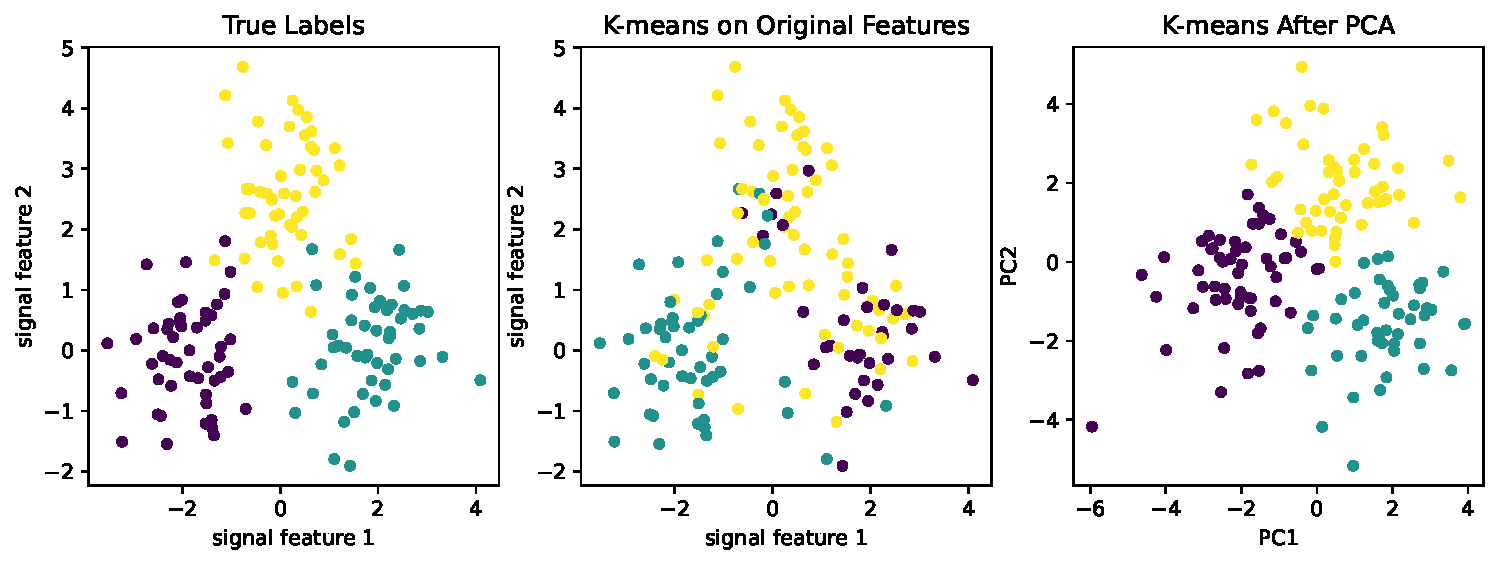
\includegraphics[keepaspectratio]{contents/3/dimensionr_files/figure-pdf/cell-20-output-1.pdf}}

This example works because the cluster signal is recoverable from the
leading PCA directions, while many noisy coordinates are reduced to a
smaller score representation.

\begin{tcolorbox}[enhanced jigsaw, arc=.35mm, bottomrule=.15mm, bottomtitle=1mm, breakable, colback=white, colbacktitle=quarto-callout-note-color!10!white, colframe=quarto-callout-note-color-frame, coltitle=black, left=2mm, leftrule=.75mm, opacityback=0, opacitybacktitle=0.6, rightrule=.15mm, title=\textcolor{quarto-callout-note-color}{\faInfo}\hspace{0.5em}{What the plot does not show}, titlerule=0mm, toprule=.15mm, toptitle=1mm]

The plots show only the two signal features so that the cluster
structure is visible. However, K-means on the original features is
applied to the full matrix \texttt{X\_cluster}, which also contains 200
noisy features. Those noisy coordinates affect the Euclidean distances
used by K-means, even though they are not drawn in the figure. After
PCA, the data are represented by two score columns, so much of the noise
influence is reduced before clustering.

\end{tcolorbox}

In practice, PCA as preprocessing should still be checked against the
downstream goal. If the cluster separation lies in a low-variance
direction, PCA may remove the relevant structure instead.

\chapter{Embedding and Visualization}\label{sec-embedding}

The previous chapter treated PCA as a low-rank representation of a data
matrix. PCA constructs new coordinates by multiplying the data matrix by
loading vectors, \(Z=XV_m\).

In this chapter, an \textbf{embedding} means a lower-dimensional
coordinate representation of the observations:

\[
x_i\in\mathbb R^p \longrightarrow z_i\in\mathbb R^m, \qquad m\ll p.
\]

\begin{tcolorbox}[enhanced jigsaw, arc=.35mm, bottomrule=.15mm, bottomtitle=1mm, breakable, colback=white, colbacktitle=quarto-callout-note-color!10!white, colframe=quarto-callout-note-color-frame, coltitle=black, left=2mm, leftrule=.75mm, opacityback=0, opacitybacktitle=0.6, rightrule=.15mm, title=\textcolor{quarto-callout-note-color}{\faInfo}\hspace{0.5em}{Three uses of the word embedding}, titlerule=0mm, toprule=.15mm, toptitle=1mm]

\begin{itemize}
\tightlist
\item
  In this chapter, an embedding is a lower-dimensional representation of
  high-dimensional observations.
\item
  In mathematics, an embedding usually means an injective map that
  preserves the relevant structure.
\item
  In language models, an embedding is a vector representation of words,
  sentences, or documents, usually designed so that similar meanings
  have nearby vectors.
\end{itemize}

These uses are related in spirit, but they are not the same mathematical
object. In this chapter, injectivity or surjectivity is not the main
issue. What matters is which relationships among observations the
embedding tries to preserve.

\end{tcolorbox}

PCA is a linear embedding: each coordinate is a feature combination, and
the axes can be interpreted through loadings. The methods in this
chapter usually build coordinates from distances, neighborhoods, or
graphs instead. Their axes are useful for visualization, but they
usually do not have direct feature interpretations.

We focus on three methods:

\begin{itemize}
\tightlist
\item
  spectral embedding, which builds coordinates from a similarity graph;
\item
  t-SNE, which matches high-dimensional and low-dimensional neighborhood
  probabilities;
\item
  UMAP, which builds and matches nearest-neighbor graphs.
\end{itemize}

The shared goal is not to reconstruct \(X\) feature by feature. The goal
is to make selected relationships among observations visible in a small
number of coordinates, usually two.

\begin{tcolorbox}[enhanced jigsaw, arc=.35mm, bottomrule=.15mm, bottomtitle=1mm, breakable, colback=white, colbacktitle=quarto-callout-caution-color!10!white, colframe=quarto-callout-caution-color-frame, coltitle=black, left=2mm, leftrule=.75mm, opacityback=0, opacitybacktitle=0.6, rightrule=.15mm, title=\textcolor{quarto-callout-caution-color}{\faFire}\hspace{0.5em}{Embeddings are task-dependent}, titlerule=0mm, toprule=.15mm, toptitle=1mm]

In this chapter, embeddings are mainly used for visualization and
sometimes for clustering. They can also be useful for other tasks, but
not every embedding is useful for every task.

The reason is that different methods preserve different relationships.
PCA preserves variance and optimizes linear reconstruction. Spectral
embedding, t-SNE, and UMAP preserve neighborhoods or graph structure in
different ways. For example, t-SNE is useful for visualizing local
neighborhoods, but distances in a t-SNE plot are not reliable enough to
automatically use as input to a distance-based method such as KNN. A
good embedding plot is therefore a guide for exploration, not a
guarantee that the coordinates are appropriate for clustering,
prediction, compression, or denoising. We will discuss these later in
more details.

\end{tcolorbox}

Because an embedding is built from the rows of \(X\), two choices come
before the algorithm itself:

\begin{itemize}
\tightlist
\item
  how each observation is represented as a row vector;
\item
  how similarity or distance between rows is defined.
\end{itemize}

Thus a common workflow is

\[
X
\longrightarrow
\text{row representation}
\longrightarrow
\text{similarity or neighborhood structure}
\longrightarrow
\text{low-dimensional embedding}.
\]

\section{Spectral Embedding}\label{spectral-embedding}

Spectral embedding starts by replacing the original data matrix with a
graph. The rows \(x_i\in\mathbb R^p\) are observations in feature space.
Spectral embedding keeps the same observations, but represents their
relationships by a graph: the vertices are observations, and edges
connect observations that are similar, often nearest neighbors.

The main idea is:

\[
X
\longrightarrow
\text{similarity graph}
\longrightarrow
\text{graph Laplacian}
\longrightarrow
\text{observation-space eigenvector coordinates}.
\]

This is useful when the structure is better described by connectivity
than by distance to a single center. Spectral clustering uses the same
embedding and then applies a label-assignment method such as K-means.

\subsection{Mathematical Idea}\label{mathematical-idea}

Let \(W=\mqty[W_{ij}]\in\mathbb R^{n\times n}\) be a symmetric weighted
adjacency matrix. A large \(W_{ij}\) means observations \(i\) and \(j\)
are strongly connected. Define the degree matrix

\[
D=\operatorname{diag}(d_1,\ldots,d_n),
\qquad
d_i=\sum_j W_{ij}.
\]

The unnormalized graph Laplacian is

\[
L=D-W.
\]

Both \(W\) and \(L\) are \(n\times n\) matrices, so they act on vectors
in observation space \(\mathbb R^n\). A vector

\[
y=\mqty[y_1,\ldots,y_n]^\top\in\mathbb R^n
\]

assigns one coordinate value to every observation. The entry \(y_i\) is
the coordinate assigned to observation \(i\).

\begin{tcolorbox}[enhanced jigsaw, arc=.35mm, bottomrule=.15mm, bottomtitle=1mm, breakable, colback=white, colbacktitle=quarto-callout-note-color!10!white, colframe=quarto-callout-note-color-frame, coltitle=black, left=2mm, leftrule=.75mm, opacityback=0, opacitybacktitle=0.6, rightrule=.15mm, title=\textcolor{quarto-callout-note-color}{\faInfo}\hspace{0.5em}{What does \(L\) do?}, titlerule=0mm, toprule=.15mm, toptitle=1mm]

The matrix \(L\) compares each observation with its neighbors in the
graph. If \(y\in\mathbb R^n\) assigns one number to each observation,
then the \(i\)-th entry of \(Ly\) is

\[
(Ly)_i
=
d_i y_i-\sum_j W_{ij}y_j
=
\sum_j W_{ij}(y_i-y_j).
\]

Thus \((Ly)_i\) is a weighted difference between the coordinate of
observation \(i\) and the coordinates of its neighbors.

\begin{itemize}
\tightlist
\item
  If \(y_i\) is close to the coordinates of strongly connected
  neighbors, then \((Ly)_i\) is small.
\item
  If \(y_i\) is very different from strongly connected neighbors, then
  \((Ly)_i\) is large.
\end{itemize}

In this sense, \(L\) measures how rough or unsmooth the coordinate
vector \(y\) is over the graph. Smooth coordinates change slowly across
strong edges.

\end{tcolorbox}

The \textbf{graph roughness} of an observation-space coordinate vector
\(y\) is

\[
\operatorname{roughness}_G(y)
=
y^\top Ly
=
\frac12\sum_{i,j}W_{ij}(y_i-y_j)^2.
\]

It measures how much the coordinate values change across graph edges,
with larger penalties on stronger edges. This expression is small when
strongly connected observations receive similar coordinates. This is
exactly the behavior we want from a graph embedding. If \(W_{ij}\) is
large, then observations \(i\) and \(j\) are strongly connected, so we
want their embedded coordinates to be close:

\[
y_i\approx y_j.
\]

The term \(W_{ij}(y_i-y_j)^2\) penalizes the opposite situation: a
strong edge with very different coordinates. Therefore minimizing
\(y^\top Ly\) means finding an observation-space coordinate column that
keeps strongly connected observations close together. In other words, we
need the eigenvectors corresponding to the smallest nonzero eigenvalues
of \(L\).

Click to expand.

\begin{center}\rule{0.5\linewidth}{0.5pt}\end{center}

More explicitly, a one-dimensional observation-space coordinate can be
described as trying to solve

\[
\min_y y^\top Ly
\qquad
\text{subject to }
\norm{y}^2=1
\text{ and }
y\perp \mathbf 1.
\]

The constraints remove trivial solutions. Without them, \(y=0\)
minimizes the objective. Even with a nonzero vector, the constant
coordinate \(y_1=\cdots=y_n\) makes every coordinate difference zero, so
it does not separate observations. The constraint \(\norm{y}^2=1\) fixes
the scale, and \(y\perp \mathbf 1\) removes the constant coordinate.

This optimization problem leads to eigenvectors because \(L\) is
symmetric. Write its orthonormal eigen-decomposition as

\[
L=V\Lambda V^\top.
\]

If \(v_1,\ldots,v_n\) are the eigenvectors of \(L\), then any unit
vector \(y\) can be expanded in this eigenbasis:

\[
y=a_1v_1+\cdots+a_nv_n,
\qquad
\sum_{k=1}^n a_k^2=1.
\]

Then

\[
y^\top Ly
=
\sum_{k=1}^n \lambda_k a_k^2.
\]

Thus \(y^\top Ly\) is a weighted average of the eigenvalues. To make it
small, we put weight on eigenvectors with small eigenvalues. For a graph
Laplacian, the smallest eigenvalue is usually \(0\), with a constant
eigenvector on each connected component. That eigenvector has zero graph
roughness, but it gives every observation the same coordinate. After
removing this constant direction, the first useful one-dimensional
spectral coordinate is the eigenvector corresponding to the smallest
positive eigenvalue:

\[
Lv=\lambda v,
\qquad
\lambda
=
\min\{\lambda_k:\lambda_k>0\}.
\]

This eigenvector \(v=\mqty[v_1,\ldots,v_n]^\top\) assigns one coordinate
value to each observation: the entry \(v_i\) becomes the new coordinate
of observation \(i\). Since

\[
v^\top Lv
=
\lambda v^\top v,
\]

the smallest positive eigenvalue gives the nonconstant coordinate with
the smallest graph roughness. Therefore strongly connected observations
tend to receive similar values. Additional spectral coordinates come
from the next smallest positive eigenvalues.

\begin{center}\rule{0.5\linewidth}{0.5pt}\end{center}

Consider the eigenvectors of the graph Laplacian \(v_1,\ldots, v_n\),
ordered by ascending eigenvalues. Each selected eigenvector gives one
coordinate column for all observations. For an \(m\)-dimensional
spectral embedding, we place the first \(m\) nonconstant eigenvectors
side by side:

\[
Z
=
\mqty[v_2 & v_3 & \cdots & v_{m+1}]
\in\mathbb R^{n\times m}.
\]

The embedding is then obtained by reading across rows of this matrix.
The \(i\)-th row of \(Z\) gives the embedded coordinate of observation
\(i\):

\[
z_i^\top
=
\mqty[v_2(i) & v_3(i) & \cdots & v_{m+1}(i)],
\]

where \(v_k(i)\) is the \(i\)-th entry of the \(k\)-th Laplacian
eigenvector. In words, observation \(i\) gets its first coordinate from
the \(i\)-th entry of \(v_2\), its second coordinate from the \(i\)-th
entry of \(v_3\), and so on.

\begin{example}[A four-point
graph]\protect\hypertarget{exm-spectral-four-points}{}\label{exm-spectral-four-points}

Suppose the original dataset has four observations and any number of
predictors:

\[
X\in\mathbb R^{4\times p}.
\]

The value of \(p\) does not matter for this example. The spectral
embedding starts after those observations have been converted into a
similarity matrix. Suppose observations 1 and 2 are strongly connected,
observations 3 and 4 are strongly connected, and observations 2 and 3
are weakly connected:

\[
W
=
\mqty[
0 & 1 & 0 & 0\\
1 & 0 & 0.2 & 0\\
0 & 0.2 & 0 & 1\\
0 & 0 & 1 & 0
].
\]

This matrix says that the graph has two strong pairs, \((1,2)\) and
\((3,4)\), with a weak bridge between observations 2 and 3. From this
matrix we form the graph Laplacian \(L=D-W\) and compute the
eigenvectors. A small nonconstant Laplacian eigenvector is approximately

\[
v_2
\approx
\mqty[
0.547\\
0.448\\
-0.448\\
-0.547
].
\]

Using \(v_2\) as a one-dimensional embedding means the output has
dimension

\[
Z\in\mathbb R^{4\times 1}.
\]

The embedding is obtained by reading the entries of \(v_2\):

\[
Z
=
v_2
\approx
\mqty[
0.547\\
0.448\\
-0.448\\
-0.547
].
\]

Thus the spectral embedding maps the original observations as follows:

\[
x_1\mapsto 0.547,\qquad
x_2\mapsto 0.448,\qquad
x_3\mapsto -0.448,\qquad
x_4\mapsto -0.547.
\]

The result tells us that observations 1 and 2 are close in the
embedding, observations 3 and 4 are close in the embedding, and there is
a large gap between the two pairs. This reflects the graph structure
encoded in \(W\): two strong within-pair connections and one weak
bridge. The coordinate is not a feature combination like \(Xv\) in PCA,
where \(v\in\mathbb R^p\) is a loading vector. It is a coordinate read
from a Laplacian eigenvector, so its values are determined by graph
connectivity.

\end{example}

\subsection{Spectral Embedding in
Python}\label{spectral-embedding-in-python}

We can use \texttt{SpectralEmbedding} from \texttt{sklearn.manifold} to
compute a spectral embedding. The first hyperparameter,
\texttt{n\_components}, specifies the dimension of the embedding.
However, it is usually not the most important hyperparameter.

As discussed earlier, spectral embedding starts by constructing a local
connectivity graph. There are several ways to construct the connectivity
matrix \(W\). One of the most common approaches is the nearest neighbors
method:

\begin{enumerate}
\def\labelenumi{\arabic{enumi}.}
\tightlist
\item
  Choose the number of nearest neighbors, \texttt{n\_neighbors}.
\item
  For each point, find its \texttt{n\_neighbors} nearest neighbors.
\item
  Set \(W_{ij}=1\) if points \(i\) and \(j\) are connected, and
  \(W_{ij}=0\) otherwise.
\end{enumerate}

This produces a sparse connectivity matrix \(W\), which is then used to
compute the graph Laplacian and the spectral embedding.

In \texttt{SpectralEmbedding}, this construction is specified by
\texttt{affinity="nearest\_neighbors"} together with the parameter
\texttt{n\_neighbors}. In practice, choosing an appropriate neighborhood
size or a different way of constructing the connectivity graph is often
more important than choosing the embedding dimension.

The formulas above use the unnormalized graph Laplacian \(L=D-W\) for
exposition. The \texttt{sklearn} implementation uses a normalized graph
Laplacian. The interpretation is the same at this level: the embedding
favors coordinates that vary smoothly over the graph, but the exact
matrix used in the computation is different.

\begin{tcolorbox}[enhanced jigsaw, arc=.35mm, bottomrule=.15mm, bottomtitle=1mm, breakable, colback=white, colbacktitle=quarto-callout-note-color!10!white, colframe=quarto-callout-note-color-frame, coltitle=black, left=2mm, leftrule=.75mm, opacityback=0, opacitybacktitle=0.6, rightrule=.15mm, title=\textcolor{quarto-callout-note-color}{\faInfo}\hspace{0.5em}{\texttt{SpectralClustering}}, titlerule=0mm, toprule=.15mm, toptitle=1mm]

A common use of spectral embedding is to apply a clustering algorithm,
such as KMeans, to the embedded coordinates. You can do this manually by
combining \texttt{SpectralEmbedding} with \texttt{KMeans}, or you can
use \texttt{SpectralClustering} from \texttt{sklearn.cluster}, which
performs these two steps automatically.

If you want to visualize the embedding itself, however, you should use
\texttt{SpectralEmbedding} directly and then apply the clustering
algorithm manually.

\end{tcolorbox}

\subsubsection{Example}\label{example-2}

We generate a dataset consisting of two concentric circles and add a
small number of bridge points connecting them. The outer circle has
uneven density, meaning that the point density varies along its
perimeter.

Although the bridge points connect the two circles geometrically, we
still regard the data as containing two clusters: the inner circle and
the outer circle. The bridge points are treated as noise rather than
evidence that the two circles belong to the same cluster.

The dataset is generated manually using NumPy because
\texttt{sklearn.datasets.make\_circles} cannot generate circles with
non-uniform point density. The dataset is visualized after generating.

\begin{Shaded}
\begin{Highlighting}[]
\ImportTok{import}\NormalTok{ numpy }\ImportTok{as}\NormalTok{ np}
\ImportTok{import}\NormalTok{ matplotlib.pyplot }\ImportTok{as}\NormalTok{ plt}

\NormalTok{n\_samples }\OperatorTok{=} \DecValTok{900}
\NormalTok{rng }\OperatorTok{=}\NormalTok{ np.random.default\_rng(}\DecValTok{0}\NormalTok{)}

\NormalTok{n\_inner }\OperatorTok{=}\NormalTok{ n\_samples }\OperatorTok{//} \DecValTok{2}
\NormalTok{n\_outer }\OperatorTok{=}\NormalTok{ n\_samples }\OperatorTok{{-}}\NormalTok{ n\_inner}

\CommentTok{\# Inner circle}
\NormalTok{theta }\OperatorTok{=}\NormalTok{ rng.uniform(}\DecValTok{0}\NormalTok{, }\DecValTok{2} \OperatorTok{*}\NormalTok{ np.pi, n\_inner)}
\NormalTok{r }\OperatorTok{=}\NormalTok{ rng.normal(}\FloatTok{1.0}\NormalTok{, }\FloatTok{0.035}\NormalTok{, n\_inner)}
\NormalTok{x\_in }\OperatorTok{=}\NormalTok{ r }\OperatorTok{*}\NormalTok{ np.cos(theta)}
\NormalTok{y\_in }\OperatorTok{=}\NormalTok{ r }\OperatorTok{*}\NormalTok{ np.sin(theta)}

\CommentTok{\# Outer circle with uneven density}
\NormalTok{theta\_out }\OperatorTok{=}\NormalTok{ []}
\ControlFlowTok{while} \BuiltInTok{len}\NormalTok{(theta\_out) }\OperatorTok{\textless{}}\NormalTok{ n\_outer:}
\NormalTok{    theta }\OperatorTok{=}\NormalTok{ rng.uniform(}\DecValTok{0}\NormalTok{, }\DecValTok{2} \OperatorTok{*}\NormalTok{ np.pi, }\DecValTok{6} \OperatorTok{*}\NormalTok{ n\_outer)}
\NormalTok{    prob }\OperatorTok{=} \FloatTok{0.08} \OperatorTok{+} \FloatTok{0.92} \OperatorTok{*}\NormalTok{ np.sin(}\FloatTok{2.5} \OperatorTok{*}\NormalTok{ theta) }\OperatorTok{**} \DecValTok{2}
\NormalTok{    keep }\OperatorTok{=}\NormalTok{ rng.random(}\BuiltInTok{len}\NormalTok{(theta)) }\OperatorTok{\textless{}}\NormalTok{ prob}
\NormalTok{    theta\_out.extend(theta[keep])}

\NormalTok{theta\_out }\OperatorTok{=}\NormalTok{ np.array(theta\_out[:n\_outer])}

\NormalTok{r }\OperatorTok{=}\NormalTok{ rng.normal(}\FloatTok{2.6}\NormalTok{, }\FloatTok{0.04}\NormalTok{, n\_outer)}
\NormalTok{x\_out }\OperatorTok{=}\NormalTok{ r }\OperatorTok{*}\NormalTok{ np.cos(theta\_out)}
\NormalTok{y\_out }\OperatorTok{=}\NormalTok{ r }\OperatorTok{*}\NormalTok{ np.sin(theta\_out)}

\NormalTok{X }\OperatorTok{=}\NormalTok{ np.vstack([}
\NormalTok{    np.column\_stack([x\_in, y\_in]),}
\NormalTok{    np.column\_stack([x\_out, y\_out]),}
\NormalTok{])}

\NormalTok{y }\OperatorTok{=}\NormalTok{ np.array([}\DecValTok{0}\NormalTok{] }\OperatorTok{*}\NormalTok{ n\_inner }\OperatorTok{+}\NormalTok{ [}\DecValTok{1}\NormalTok{] }\OperatorTok{*}\NormalTok{ n\_outer)}

\CommentTok{\# Bridge points}
\NormalTok{n\_bridge }\OperatorTok{=} \DecValTok{10}
\NormalTok{theta }\OperatorTok{=}\NormalTok{ rng.normal(}\FloatTok{0.4}\NormalTok{, }\FloatTok{0.02}\NormalTok{, n\_bridge)}
\NormalTok{r }\OperatorTok{=}\NormalTok{ np.linspace(}\FloatTok{1.05}\NormalTok{, }\FloatTok{2.55}\NormalTok{, n\_bridge)}
\NormalTok{r }\OperatorTok{+=}\NormalTok{ rng.normal(}\DecValTok{0}\NormalTok{, }\FloatTok{0.02}\NormalTok{, n\_bridge)}

\NormalTok{x }\OperatorTok{=}\NormalTok{ r }\OperatorTok{*}\NormalTok{ np.cos(theta)}
\NormalTok{y\_bridge }\OperatorTok{=}\NormalTok{ r }\OperatorTok{*}\NormalTok{ np.sin(theta)}

\NormalTok{X\_bridge }\OperatorTok{=}\NormalTok{ np.column\_stack([x, y\_bridge])}

\CommentTok{\# Assign each bridge point to the nearest circle}
\NormalTok{labels }\OperatorTok{=}\NormalTok{ (np.}\BuiltInTok{abs}\NormalTok{(r }\OperatorTok{{-}} \FloatTok{1.0}\NormalTok{) }\OperatorTok{\textgreater{}}\NormalTok{ np.}\BuiltInTok{abs}\NormalTok{(r }\OperatorTok{{-}} \FloatTok{2.6}\NormalTok{)).astype(}\BuiltInTok{int}\NormalTok{)}

\NormalTok{X }\OperatorTok{=}\NormalTok{ np.vstack([X, X\_bridge])}
\NormalTok{y }\OperatorTok{=}\NormalTok{ np.concatenate([y, labels])}

\NormalTok{plt.scatter(X[:, }\DecValTok{0}\NormalTok{], X[:, }\DecValTok{1}\NormalTok{], c}\OperatorTok{=}\NormalTok{y, s}\OperatorTok{=}\DecValTok{8}\NormalTok{)}
\NormalTok{plt.title(}\StringTok{"Ground Truth"}\NormalTok{)}
\NormalTok{plt.xticks([])}
\NormalTok{plt.yticks([])}
\NormalTok{plt.axis(}\StringTok{"equal"}\NormalTok{)}\OperatorTok{;}
\end{Highlighting}
\end{Shaded}

\pandocbounded{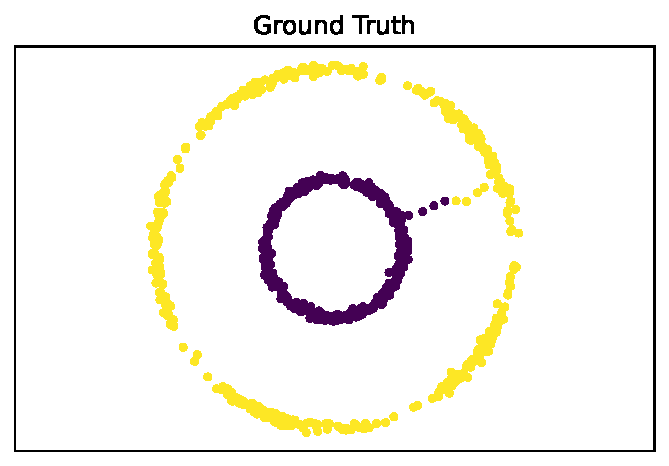
\includegraphics[keepaspectratio]{contents/3/embedding_files/figure-pdf/cell-2-output-1.pdf}}

Now we apply the four clustering methods and compare their results.
Since the true labels are available, we use the adjusted Rand index
(ARI) to evaluate the clustering performance.

For all methods, the hyperparameters were only tuned lightly rather than
exhaustively. Better performance may be achievable with more careful
tuning, but the overall conclusions are unlikely to change. The purpose
of this example is not to compare the best possible performance of each
algorithm, but to illustrate their typical behavior on this dataset.

\begin{Shaded}
\begin{Highlighting}[]
\ImportTok{from}\NormalTok{ sklearn.cluster }\ImportTok{import}\NormalTok{ KMeans, AgglomerativeClustering, DBSCAN}
\ImportTok{from}\NormalTok{ sklearn.manifold }\ImportTok{import}\NormalTok{ SpectralEmbedding}

\NormalTok{kmeans\_labels }\OperatorTok{=}\NormalTok{ KMeans(n\_clusters}\OperatorTok{=}\DecValTok{2}\NormalTok{, n\_init}\OperatorTok{=}\DecValTok{10}\NormalTok{, random\_state}\OperatorTok{=}\DecValTok{0}\NormalTok{).fit\_predict(X)}

\NormalTok{ha\_labels }\OperatorTok{=}\NormalTok{ AgglomerativeClustering(n\_clusters}\OperatorTok{=}\DecValTok{2}\NormalTok{, linkage}\OperatorTok{=}\StringTok{"ward"}\NormalTok{).fit\_predict(X)}

\NormalTok{dbscan\_labels }\OperatorTok{=}\NormalTok{ DBSCAN(eps}\OperatorTok{=}\FloatTok{0.5}\NormalTok{, min\_samples}\OperatorTok{=}\DecValTok{10}\NormalTok{).fit\_predict(X)}

\NormalTok{Z }\OperatorTok{=}\NormalTok{ SpectralEmbedding(n\_components}\OperatorTok{=}\DecValTok{2}\NormalTok{, n\_neighbors}\OperatorTok{=}\DecValTok{15}\NormalTok{, random\_state}\OperatorTok{=}\DecValTok{0}\NormalTok{).fit\_transform(X)}
\NormalTok{spectral\_labels }\OperatorTok{=}\NormalTok{ KMeans(n\_clusters}\OperatorTok{=}\DecValTok{2}\NormalTok{, random\_state}\OperatorTok{=}\DecValTok{0}\NormalTok{, n\_init}\OperatorTok{=}\DecValTok{10}\NormalTok{).fit\_predict(Z)}
\end{Highlighting}
\end{Shaded}

\begin{Shaded}
\begin{Highlighting}[]
\ImportTok{from}\NormalTok{ sklearn.metrics }\ImportTok{import}\NormalTok{ adjusted\_rand\_score}

\NormalTok{labels }\OperatorTok{=}\NormalTok{ \{}
    \StringTok{"KMeans"}\NormalTok{: kmeans\_labels,}
    \StringTok{"Agglomerative (Ward)"}\NormalTok{: ha\_labels,}
    \StringTok{"DBSCAN"}\NormalTok{: dbscan\_labels,}
    \StringTok{"Spectral Clustering"}\NormalTok{: spectral\_labels,}
\NormalTok{\}}
\NormalTok{results }\OperatorTok{=}\NormalTok{ \{}
\NormalTok{    name: (label, adjusted\_rand\_score(y, label)) }\ControlFlowTok{for}\NormalTok{ name, label }\KeywordTok{in}\NormalTok{ labels.items()}
\NormalTok{\}}

\NormalTok{fig, axes }\OperatorTok{=}\NormalTok{ plt.subplots(}\DecValTok{2}\NormalTok{, }\DecValTok{2}\NormalTok{, figsize}\OperatorTok{=}\NormalTok{(}\DecValTok{10}\NormalTok{, }\DecValTok{10}\NormalTok{))}
\NormalTok{axes }\OperatorTok{=}\NormalTok{ axes.ravel()}

\ControlFlowTok{for}\NormalTok{ ax, (name, (labels, ari)) }\KeywordTok{in} \BuiltInTok{zip}\NormalTok{(axes, results.items()):}
\NormalTok{    ax.scatter(X[:, }\DecValTok{0}\NormalTok{], X[:, }\DecValTok{1}\NormalTok{], c}\OperatorTok{=}\NormalTok{labels, s}\OperatorTok{=}\DecValTok{8}\NormalTok{)}
\NormalTok{    ax.set\_title(}\SpecialStringTok{f"}\SpecialCharTok{\{}\NormalTok{name}\SpecialCharTok{\}}\CharTok{\textbackslash{}n}\SpecialStringTok{ARI = }\SpecialCharTok{\{}\NormalTok{ari}\SpecialCharTok{:.3f\}}\SpecialStringTok{"}\NormalTok{, fontsize}\OperatorTok{=}\DecValTok{13}\NormalTok{)}

\NormalTok{    ax.set\_xticks([])}
\NormalTok{    ax.set\_yticks([])}
\NormalTok{    ax.set\_aspect(}\StringTok{"equal"}\NormalTok{)}\OperatorTok{;}
\end{Highlighting}
\end{Shaded}

\pandocbounded{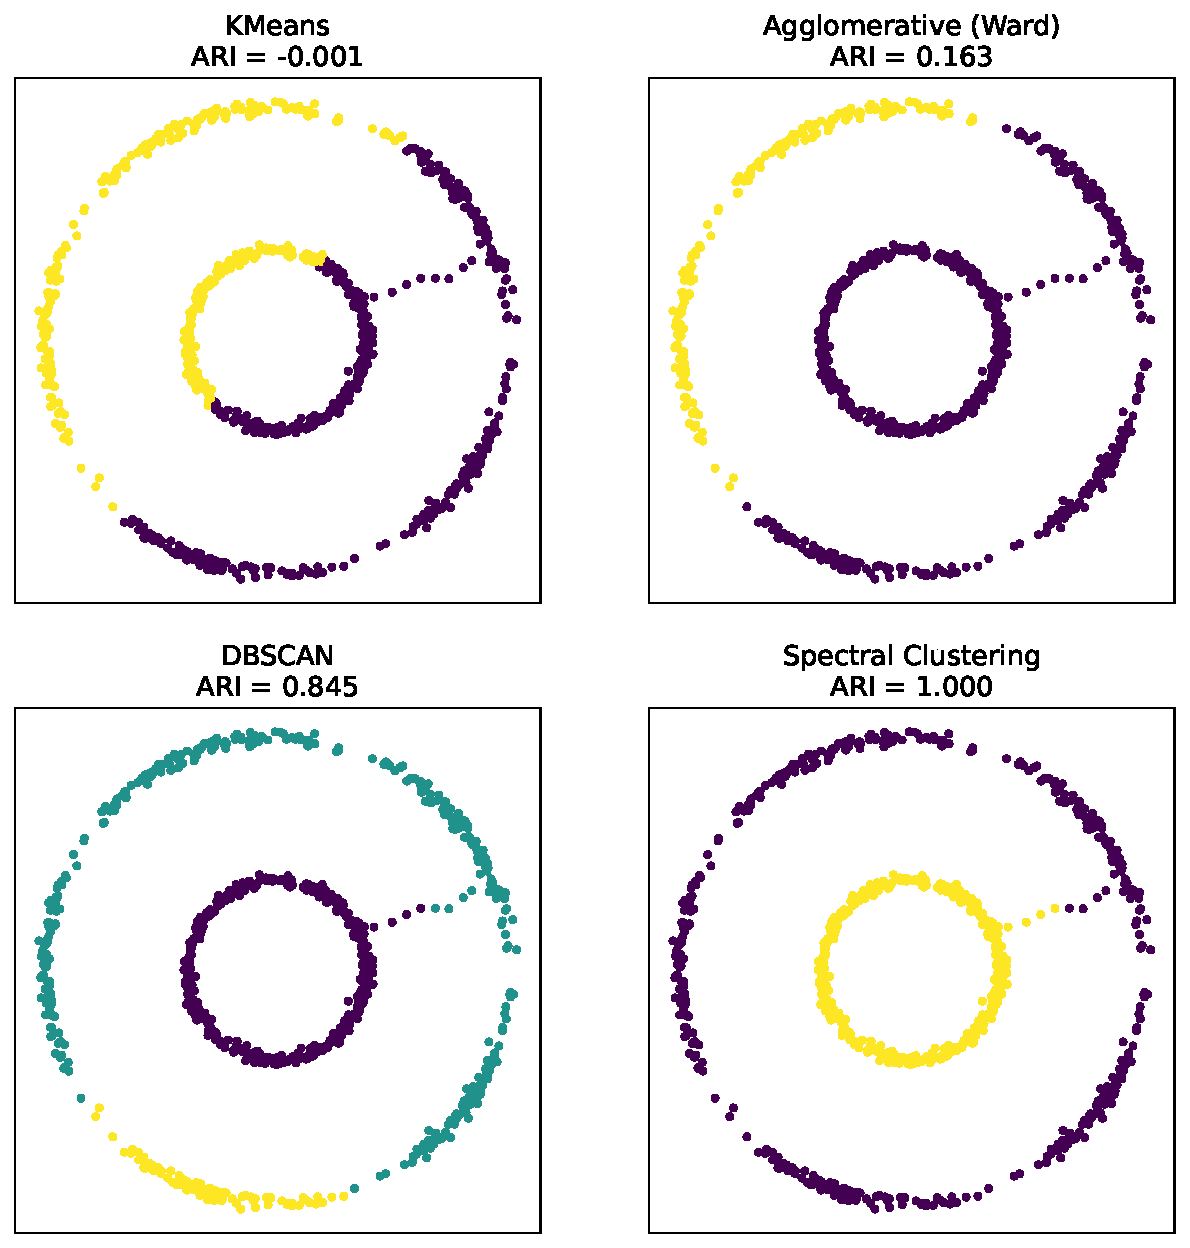
\includegraphics[keepaspectratio]{contents/3/embedding_files/figure-pdf/cell-4-output-1.pdf}}

The results illustrate the different assumptions made by the clustering
algorithms.

\begin{itemize}
\tightlist
\item
  KMeans: Fails. KMeans partitions the data according to the distance to
  cluster centroids. Since the two circles share the same center, the
  algorithm cannot separate them into inner and outer circles. Instead,
  it splits the data into two roughly equal halves.
\item
  Agglomerative (Ward): Performs slightly better but still fails. Ward
  linkage merges clusters to minimize the increase in within-cluster
  variance. This favors compact, approximately spherical clusters rather
  than ring-shaped clusters, so it also tends to cut across the circles
  instead of preserving their circular structure.
\item
  DBSCAN: Performs reasonably well but is affected by the bridge points.
  Since DBSCAN defines clusters through density connectivity, the bridge
  creates a path between the two circles, causing some points to be
  merged incorrectly. Furthermore, because DBSCAN uses a single density
  threshold, it struggles with the uneven density of the outer circle
  and fails to identify it as one cluster.
\item
  Spectral Clustering: Correctly recovers the two circles. Instead of
  clustering the original coordinates directly, it first constructs a
  similarity graph and computes a spectral embedding. In this new
  representation, points belonging to the same circle become much
  closer, while the weak bridge has little influence. A simple
  clustering algorithm such as KMeans can then easily separate the two
  clusters.
\end{itemize}

The key idea is that spectral clustering does not rely on Euclidean
geometry in the original feature space. Instead, it transforms the data
into a new space where the cluster structure becomes much easier to
identify.

The figure below shows the two-dimensional spectral embedding. Although
the circles are not linearly separable in the original space, they
become well separated after the embedding, making KMeans sufficient to
recover the correct clusters.

\begin{Shaded}
\begin{Highlighting}[]
\NormalTok{plt.scatter(Z[:, }\DecValTok{0}\NormalTok{], Z[:, }\DecValTok{1}\NormalTok{], c}\OperatorTok{=}\NormalTok{y, s}\OperatorTok{=}\DecValTok{8}\NormalTok{)}
\NormalTok{plt.title(}\StringTok{"Spectral Embedding"}\NormalTok{)}
\NormalTok{plt.xticks([])}
\NormalTok{plt.yticks([])}
\NormalTok{plt.axis(}\StringTok{"equal"}\NormalTok{)}\OperatorTok{;}
\end{Highlighting}
\end{Shaded}

\pandocbounded{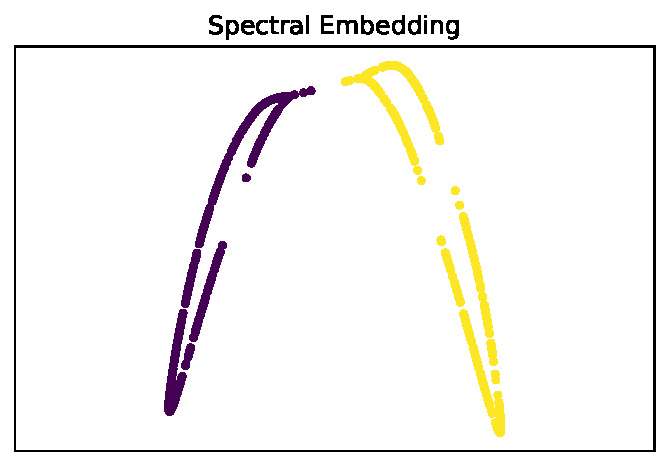
\includegraphics[keepaspectratio]{contents/3/embedding_files/figure-pdf/cell-5-output-1.pdf}}

\section{t-SNE}\label{t-sne}

t-SNE stands for t-distributed Stochastic Neighbor Embedding. It is
designed mainly for visualization. It does not try to reconstruct the
original features and does not produce interpretable axes. Instead, it
tries to preserve local neighborhoods.

The main idea is:

\[
X
\longrightarrow
\text{high-dimensional neighbor probabilities } P
\longrightarrow
\text{low-dimensional coordinates with probabilities } Q.
\]

\subsection{Mathematical Idea}\label{mathematical-idea-1}

The core algorithm is simple:

\begin{enumerate}
\def\labelenumi{\arabic{enumi}.}
\tightlist
\item
  Compute pairwise similarities among the original observations
  \(x_1,\ldots,x_n\). These similarities are converted into a
  probability matrix \(P=(p_{ij})\), where larger \(p_{ij}\) means that
  observations \(i\) and \(j\) are close neighbors in the original
  space.
\item
  Introduce low-dimensional coordinates \(z_1,\ldots,z_n\). These
  coordinates are the unknown variables that t-SNE must solve for.
\item
  From the distances among the current \(z_i\)'s, compute another
  probability matrix \(Q=(q_{ij})\). Larger \(q_{ij}\) means that points
  \(i\) and \(j\) are close in the low-dimensional display. Note that
  \(Q\) is a function of \(Z=(z_1,\ldots,z_n)\).
\item
  Adjust all coordinates \(z_1,\ldots,z_n\) so that \(Q\) is close to
  \(P\) in the sense of Kullback-Leibler divergence.
\end{enumerate}

Thus t-SNE chooses the plotted coordinates by solving

\[
\min_{z_1,\ldots,z_n}
\operatorname{KL}(P\Vert Q(z_1,\ldots,z_n)),
\]

where

\[
\operatorname{KL}(P\Vert Q)
=
\sum_{i\ne j} p_{ij}\log\qty(\frac{p_{ij}}{q_{ij}}).
\]

In practice, the coordinates are initialized, often randomly or from
PCA, and then updated by gradient descent. The next formulas define the
two probability matrices \(P\) and \(Q\) in detail.

\begin{tcolorbox}[enhanced jigsaw, arc=.35mm, bottomrule=.15mm, bottomtitle=1mm, breakable, colback=white, colbacktitle=quarto-callout-note-color!10!white, colframe=quarto-callout-note-color-frame, coltitle=black, left=2mm, leftrule=.75mm, opacityback=0, opacitybacktitle=0.6, rightrule=.15mm, title=\textcolor{quarto-callout-note-color}{\faInfo}\hspace{0.5em}{How t-SNE builds \(P\)}, titlerule=0mm, toprule=.15mm, toptitle=1mm]

For each observation \(i\), t-SNE defines the probability that \(i\)
chooses observation \(j\) as a neighbor:

\[
p_{j\mid i}
=
\frac{
\exp\qty(-\norm{x_i-x_j}^2/(2\sigma_i^2))
}{
\sum_{k\ne i}
\exp\qty(-\norm{x_i-x_k}^2/(2\sigma_i^2))
},
\qquad j\ne i.
\]

The conditional probabilities are then symmetrized to produce
\(p_{ij}\), where \(n\) is the number of observations:

\[
p_{ij}=\frac{1}{2n}(p_{i\mid j}+p_{j\mid i}).
\]

Geometrically, \(p_{ij}\) summarizes the relationship between \(x_i\)
and \(x_j\) in the original high-dimensional space. If \(x_i\) and
\(x_j\) are close relative to the local scale around them, then
\(p_{ij}\) is large.

\end{tcolorbox}

\begin{tcolorbox}[enhanced jigsaw, arc=.35mm, bottomrule=.15mm, bottomtitle=1mm, breakable, colback=white, colbacktitle=quarto-callout-note-color!10!white, colframe=quarto-callout-note-color-frame, coltitle=black, left=2mm, leftrule=.75mm, opacityback=0, opacitybacktitle=0.6, rightrule=.15mm, title=\textcolor{quarto-callout-note-color}{\faInfo}\hspace{0.5em}{How t-SNE builds \(Q\)}, titlerule=0mm, toprule=.15mm, toptitle=1mm]

For low-dimensional coordinates \(z_i\), t-SNE defines similarities
using a heavy-tailed Student-\(t\) kernel:

\[
q_{ij}
=
\frac{(1+\norm{z_i-z_j}^2)^{-1}}
{\sum_{k\ne \ell}(1+\norm{z_k-z_\ell}^2)^{-1}}.
\]

Geometrically, \(q_{ij}\) summarizes the relationship between the
plotted points \(z_i\) and \(z_j\). If the two plotted points are close,
then \(q_{ij}\) is large; if they are far apart, then \(q_{ij}\) is
small.

\end{tcolorbox}

\begin{tcolorbox}[enhanced jigsaw, arc=.35mm, bottomrule=.15mm, bottomtitle=1mm, breakable, colback=white, colbacktitle=quarto-callout-note-color!10!white, colframe=quarto-callout-note-color-frame, coltitle=black, left=2mm, leftrule=.75mm, opacityback=0, opacitybacktitle=0.6, rightrule=.15mm, title=\textcolor{quarto-callout-note-color}{\faInfo}\hspace{0.5em}{Perplexity}, titlerule=0mm, toprule=.15mm, toptitle=1mm]

\texttt{perplexity} can be read as an effective neighborhood size. It
controls how many neighbors each point effectively pays attention to.

\begin{itemize}
\tightlist
\item
  Larger \texttt{perplexity} means a broader neighborhood. The
  probability distribution \(p_{\cdot\mid i}\) is flatter and spreads
  mass over more nearby observations. This corresponds to a larger
  \(\sigma_i\).
\item
  Smaller \texttt{perplexity} means a more local neighborhood. The
  probability distribution \(p_{\cdot\mid i}\) concentrates more
  strongly on the closest observations. This corresponds to a smaller
  \(\sigma_i\).
\end{itemize}

More precisely, for each point \(i\), t-SNE chooses \(\sigma_i\) so that
the entropy of the conditional distribution \(p_{\cdot\mid i}\) matches
the requested perplexity:

\[
\operatorname{Perp}(p_{\cdot\mid i})
=
2^{H(p_{\cdot\mid i})},
\qquad
H(p_{\cdot\mid i})
=
-\sum_{j\ne i} p_{j\mid i}\log_2 p_{j\mid i}.
\]

Thus the user fixes one common \texttt{perplexity} value, while t-SNE
solves a separate \(\sigma_i\) for each observation. The \(\sigma_i\)
values can differ, allowing dense and sparse regions to use different
local distance scales while keeping the same effective neighborhood
size.

\end{tcolorbox}

\subsection{What structure does t-SNE
preserve?}\label{what-structure-does-t-sne-preserve}

t-SNE converts geometry into probabilities.

\begin{itemize}
\tightlist
\item
  The matrix \(P=(p_{ij})\) describes neighborhood relationships in the
  original high-dimensional space: nearby observations have larger
  \(p_{ij}\), and faraway observations have smaller \(p_{ij}\).
\item
  The matrix \(Q=(q_{ij})\) describes neighborhood relationships in the
  low-dimensional plot in the same way.
\end{itemize}

Minimizing \(\operatorname{KL}(P\Vert Q)\) tries to make these two
probability patterns match.

The direction of the KL divergence matters.

\begin{itemize}
\tightlist
\item
  The term \(p_{ij}\log(p_{ij}/q_{ij})\) strongly penalizes the case
  where \(p_{ij}\) is large but \(q_{ij}\) is small. Thus, if two
  observations are close neighbors in the original space, t-SNE tries
  hard to keep them close in the plot.
\item
  The converse is weaker: if two points appear close in the t-SNE plot,
  they were not necessarily close in the original space. Pairs with very
  small \(p_{ij}\) contribute little directly to the objective, so t-SNE
  is less strict about the exact arrangement of points that were already
  far apart.
\end{itemize}

Thus t-SNE preserves local neighborhood probabilities, not the original
coordinates, not the original Euclidean distances, and not the meanings
of the original features. In plain language:

\begin{itemize}
\tightlist
\item
  Original-space neighbors are likely to remain close in the t-SNE plot.
\item
  Points that are close in the t-SNE plot are not guaranteed to have
  been close in the original space.
\item
  A visible t-SNE patch may contain several real subgroups.
\item
  Distances between separated patches, patch sizes, empty space,
  orientation, and apparent density should not be used as quantitative
  evidence.
\end{itemize}

So t-SNE answers a local question: ``which observations are neighbors of
which other observations?'' It does not faithfully answer global metric
questions such as ``how far apart are these two groups?'' or ``which
visual cluster is larger or denser?''

\begin{tcolorbox}[enhanced jigsaw, arc=.35mm, bottomrule=.15mm, bottomtitle=1mm, breakable, colback=white, colbacktitle=quarto-callout-note-color!10!white, colframe=quarto-callout-note-color-frame, coltitle=black, left=2mm, leftrule=.75mm, opacityback=0, opacitybacktitle=0.6, rightrule=.15mm, title=\textcolor{quarto-callout-note-color}{\faInfo}\hspace{0.5em}{t-SNE as a diagnostic plot}, titlerule=0mm, toprule=.15mm, toptitle=1mm]

The main use of t-SNE is visualization after dimension reduction. It is
not usually used as a feature representation for a downstream model.
Instead, it helps us inspect whether patterns found by other methods are
visible in local neighborhood structure.

For example, after fitting a clustering algorithm in the original
feature space, we can color a t-SNE plot by the cluster labels. If the
colors form well-separated local patches, then the clustering is
consistent with the neighborhood structure shown by t-SNE. If the colors
are heavily mixed, then the clustering may be failing to capture local
structure, or the data may not contain clearly separated groups.

This is a diagnostic check, not a proof. t-SNE can make separation look
stronger than it really is, and the apparent distance between colored
patches is not a quantitative cluster separation. Quantitative measures
such as nearest-neighbor overlap, trustworthiness, silhouette score, or
adjusted Rand index should be used when a formal comparison is needed.
The plot is useful because it makes possible problems visible quickly.

\end{tcolorbox}

\subsection{t-SNE in Python}\label{t-sne-in-python}

We may use \texttt{TSNE} from \texttt{sklearn.manifold} to compute a
t-SNE embedding. Unlike PCA or many other sklearn transformers, standard
\texttt{sklearn} t-SNE does not provide a \texttt{.transform()} method
for new observations. The usual workflow is to fit the embedding and
return the plotted coordinates directly with \texttt{.fit\_transform()}.

\begin{Shaded}
\begin{Highlighting}[]
\ImportTok{from}\NormalTok{ sklearn.manifold }\ImportTok{import}\NormalTok{ TSNE}

\NormalTok{tsne }\OperatorTok{=}\NormalTok{ TSNE(}
\NormalTok{    n\_components}\OperatorTok{=}\DecValTok{2}\NormalTok{,}
\NormalTok{    perplexity}\OperatorTok{=}\DecValTok{30}\NormalTok{,}
\NormalTok{    init}\OperatorTok{=}\StringTok{"pca"}\NormalTok{,}
\NormalTok{    learning\_rate}\OperatorTok{=}\StringTok{"auto"}\NormalTok{,}
\NormalTok{    random\_state}\OperatorTok{=}\DecValTok{1}
\NormalTok{)}
\NormalTok{Z }\OperatorTok{=}\NormalTok{ tsne.fit\_transform(X)}
\end{Highlighting}
\end{Shaded}

The parameter \texttt{n\_components=2} asks for a two-dimensional
display. \texttt{perplexity=30} sets the effective neighborhood size
used when constructing the high-dimensional probabilities. The argument
\texttt{init="pca"} specifies how the optimization is initialized. Since
t-SNE minimizes its objective by an iterative optimization method, the
low-dimensional coordinates must be assigned initial values before the
optimization begins. Two common choices are random initialization
(\texttt{init="random"}) and PCA initialization (\texttt{init="pca"}).
We set \texttt{init="pca"} explicitly here.

With PCA initialization, the optimization starts from the coordinates
obtained by projecting the data onto the first \texttt{n\_components}
principal components. In other words, the PCA embedding serves as the
initial low-dimensional representation, and t-SNE then refines these
coordinates to minimize its own objective. PCA initialization often
converges faster and gives more stable results than random
initialization. It can also make the early layout reflect some broad
linear structure. However, it does not guarantee a better final
embedding.

The initialization is not the same as the objective. t-SNE still
optimizes the t-SNE loss after initialization. However, because the
optimization is nonconvex, different initializations can lead to
different local solutions. This is one reason to check whether visible
patterns are stable across reasonable settings.

\begin{tcolorbox}[enhanced jigsaw, arc=.35mm, bottomrule=.15mm, bottomtitle=1mm, breakable, colback=white, colbacktitle=quarto-callout-note-color!10!white, colframe=quarto-callout-note-color-frame, coltitle=black, left=2mm, leftrule=.75mm, opacityback=0, opacitybacktitle=0.6, rightrule=.15mm, title=\textcolor{quarto-callout-note-color}{\faInfo}\hspace{0.5em}{PCA initialization vs.~PCA preprocessing}, titlerule=0mm, toprule=.15mm, toptitle=1mm]

Do not confuse \texttt{init="pca"} with applying PCA before t-SNE.

\begin{itemize}
\tightlist
\item
  \texttt{init="pca"} uses a PCA embedding only as the initial values
  for gradient descent. The neighborhood probabilities are still
  computed from the data passed to \texttt{TSNE}.
\item
  Applying PCA before t-SNE replaces the original data with a
  lower-dimensional representation (for example, 50 principal
  components). In this case, t-SNE computes neighborhood probabilities
  from the PCA-transformed data.
\end{itemize}

The latter is often recommended for high-dimensional datasets because it
can reduce noise and speed up computation. The idea is to use PCA as a
preliminary compression step, often to 30 or 50 dimensions, and then let
t-SNE perform the main nonlinear embedding from that cleaner
representation.

\end{tcolorbox}

\subsection{Digits example}\label{digits-example}

We use the handwritten digits data from \texttt{sklearn} as an example.
The data have 64 pixel features. We standardize the features, reduce
them to 30 PCA coordinates, and then run t-SNE. The labels are used only
for coloring the final plot.

\begin{Shaded}
\begin{Highlighting}[]
\ImportTok{from}\NormalTok{ sklearn.datasets }\ImportTok{import}\NormalTok{ load\_digits}
\ImportTok{from}\NormalTok{ sklearn.preprocessing }\ImportTok{import}\NormalTok{ StandardScaler}
\ImportTok{from}\NormalTok{ sklearn.decomposition }\ImportTok{import}\NormalTok{ PCA}
\ImportTok{from}\NormalTok{ sklearn.manifold }\ImportTok{import}\NormalTok{ TSNE}

\NormalTok{digits }\OperatorTok{=}\NormalTok{ load\_digits()}
\NormalTok{X\_digits }\OperatorTok{=}\NormalTok{ StandardScaler().fit\_transform(digits.data)}
\NormalTok{y\_digits }\OperatorTok{=}\NormalTok{ digits.target}

\NormalTok{X\_digits\_pca }\OperatorTok{=}\NormalTok{ PCA(n\_components}\OperatorTok{=}\DecValTok{30}\NormalTok{, random\_state}\OperatorTok{=}\DecValTok{1}\NormalTok{).fit\_transform(X\_digits)}

\NormalTok{tsne }\OperatorTok{=}\NormalTok{ TSNE(}
\NormalTok{    n\_components}\OperatorTok{=}\DecValTok{2}\NormalTok{,}
\NormalTok{    perplexity}\OperatorTok{=}\DecValTok{30}\NormalTok{,}
\NormalTok{    init}\OperatorTok{=}\StringTok{"pca"}\NormalTok{,}
\NormalTok{    learning\_rate}\OperatorTok{=}\StringTok{"auto"}\NormalTok{,}
\NormalTok{    random\_state}\OperatorTok{=}\DecValTok{1}\NormalTok{,}
\NormalTok{)}
\NormalTok{Z\_tsne }\OperatorTok{=}\NormalTok{ tsne.fit\_transform(X\_digits\_pca)}
\end{Highlighting}
\end{Shaded}

\begin{Shaded}
\begin{Highlighting}[]
\ImportTok{import}\NormalTok{ matplotlib.pyplot }\ImportTok{as}\NormalTok{ plt}

\NormalTok{fig, ax }\OperatorTok{=}\NormalTok{ plt.subplots(figsize}\OperatorTok{=}\NormalTok{(}\DecValTok{8}\NormalTok{, }\DecValTok{6}\NormalTok{))}
\NormalTok{scatter }\OperatorTok{=}\NormalTok{ ax.scatter(Z\_tsne[:, }\DecValTok{0}\NormalTok{], Z\_tsne[:, }\DecValTok{1}\NormalTok{], c}\OperatorTok{=}\NormalTok{y\_digits, cmap}\OperatorTok{=}\StringTok{"tab10"}\NormalTok{, s}\OperatorTok{=}\DecValTok{10}\NormalTok{)}
\NormalTok{ax.set\_xlabel(}\StringTok{"t{-}SNE1"}\NormalTok{)}
\NormalTok{ax.set\_ylabel(}\StringTok{"t{-}SNE2"}\NormalTok{)}
\NormalTok{ax.set\_title(}\StringTok{"Digits t{-}SNE"}\NormalTok{)}
\NormalTok{ax.legend(}\OperatorTok{*}\NormalTok{scatter.legend\_elements(), title}\OperatorTok{=}\StringTok{"digit"}\NormalTok{, ncol}\OperatorTok{=}\DecValTok{2}\NormalTok{)}
\end{Highlighting}
\end{Shaded}

\pandocbounded{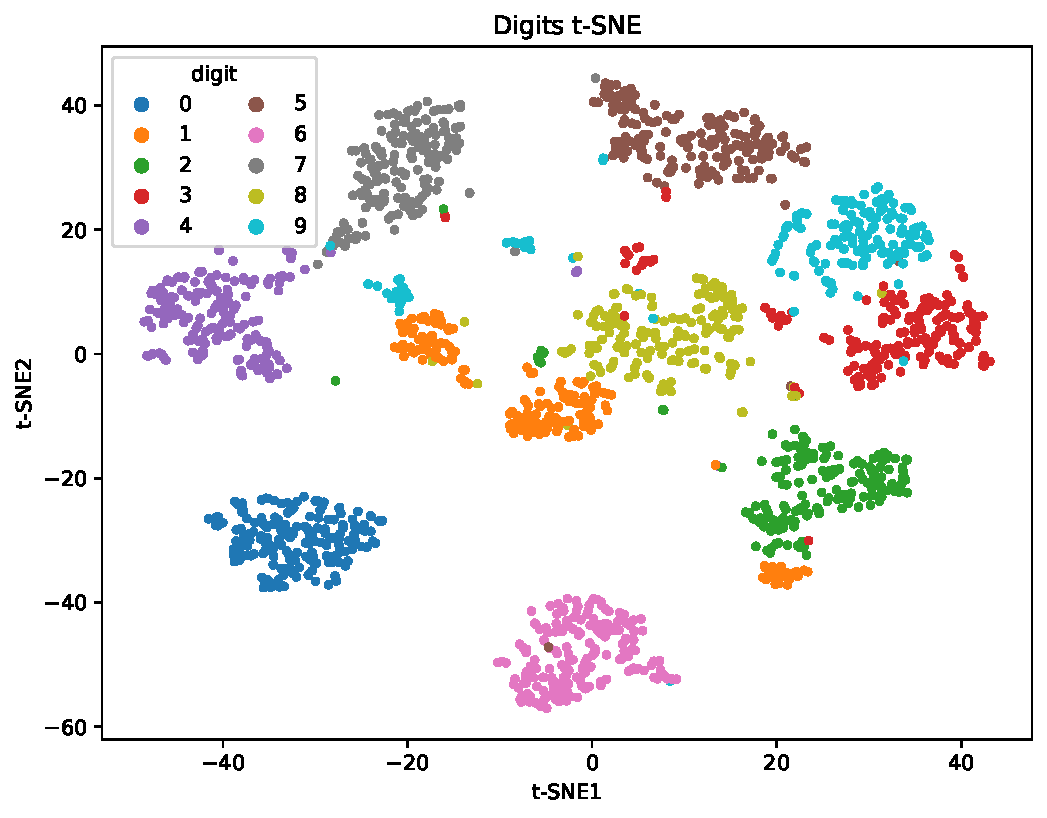
\includegraphics[keepaspectratio]{contents/3/embedding_files/figure-pdf/cell-7-output-1.pdf}}

In this example, we use \texttt{perplexity=30}, a common starting point
for a moderate-size dataset. This value should be treated as a tuning
choice rather than a fixed default.

In practice, choose \texttt{perplexity} by comparing several reasonable
values. For a moderate-size dataset, values such as \texttt{5},
\texttt{10}, \texttt{30}, and \texttt{50} are common candidates. Use
smaller values when you want to emphasize very local neighborhoods, and
larger values when you want a smoother display based on broader
neighborhoods. The chosen \texttt{perplexity} should be well below the
sample size. The result can also depend on initialization and random
seed, so a pattern is more credible when it persists across several
reasonable \texttt{perplexity} values and random seeds.

\subsection{\texorpdfstring{More about
\texttt{perplexity}}{More about perplexity}}\label{more-about-perplexity}

The plots below use the same preprocessed digits data and the same
random seed, but change \texttt{perplexity}.

\begin{Shaded}
\begin{Highlighting}[]
\NormalTok{perplexities }\OperatorTok{=}\NormalTok{ [}\DecValTok{5}\NormalTok{, }\DecValTok{10}\NormalTok{, }\DecValTok{30}\NormalTok{, }\DecValTok{50}\NormalTok{]}

\NormalTok{fig, axs }\OperatorTok{=}\NormalTok{ plt.subplots(}\DecValTok{2}\NormalTok{, }\DecValTok{2}\NormalTok{, figsize}\OperatorTok{=}\NormalTok{(}\DecValTok{10}\NormalTok{, }\DecValTok{8}\NormalTok{))}
\NormalTok{scatter }\OperatorTok{=} \VariableTok{None}

\ControlFlowTok{for}\NormalTok{ ax, perplexity }\KeywordTok{in} \BuiltInTok{zip}\NormalTok{(axs.ravel(), perplexities):}
\NormalTok{    model }\OperatorTok{=}\NormalTok{ TSNE(}
\NormalTok{        n\_components}\OperatorTok{=}\DecValTok{2}\NormalTok{,}
\NormalTok{        perplexity}\OperatorTok{=}\NormalTok{perplexity,}
\NormalTok{        init}\OperatorTok{=}\StringTok{"pca"}\NormalTok{,}
\NormalTok{        learning\_rate}\OperatorTok{=}\StringTok{"auto"}\NormalTok{,}
\NormalTok{        random\_state}\OperatorTok{=}\DecValTok{1}\NormalTok{,}
\NormalTok{    )}
\NormalTok{    Z }\OperatorTok{=}\NormalTok{ model.fit\_transform(X\_digits\_pca)}
\NormalTok{    scatter }\OperatorTok{=}\NormalTok{ ax.scatter(Z[:, }\DecValTok{0}\NormalTok{], Z[:, }\DecValTok{1}\NormalTok{], c}\OperatorTok{=}\NormalTok{y\_digits, cmap}\OperatorTok{=}\StringTok{"tab10"}\NormalTok{, s}\OperatorTok{=}\DecValTok{8}\NormalTok{)}
\NormalTok{    ax.set\_title(}\SpecialStringTok{f"perplexity = }\SpecialCharTok{\{}\NormalTok{perplexity}\SpecialCharTok{\}}\SpecialStringTok{"}\NormalTok{)}
\NormalTok{    ax.set\_xticks([])}
\NormalTok{    ax.set\_yticks([])}

\NormalTok{fig.legend(}
    \OperatorTok{*}\NormalTok{scatter.legend\_elements(),}
\NormalTok{    title}\OperatorTok{=}\StringTok{"digit"}\NormalTok{,}
\NormalTok{    loc}\OperatorTok{=}\StringTok{"center right"}\NormalTok{,}
\NormalTok{)}
\NormalTok{fig.tight\_layout(rect}\OperatorTok{=}\NormalTok{[}\DecValTok{0}\NormalTok{, }\DecValTok{0}\NormalTok{, }\FloatTok{0.9}\NormalTok{, }\DecValTok{1}\NormalTok{])}\OperatorTok{;}
\end{Highlighting}
\end{Shaded}

\pandocbounded{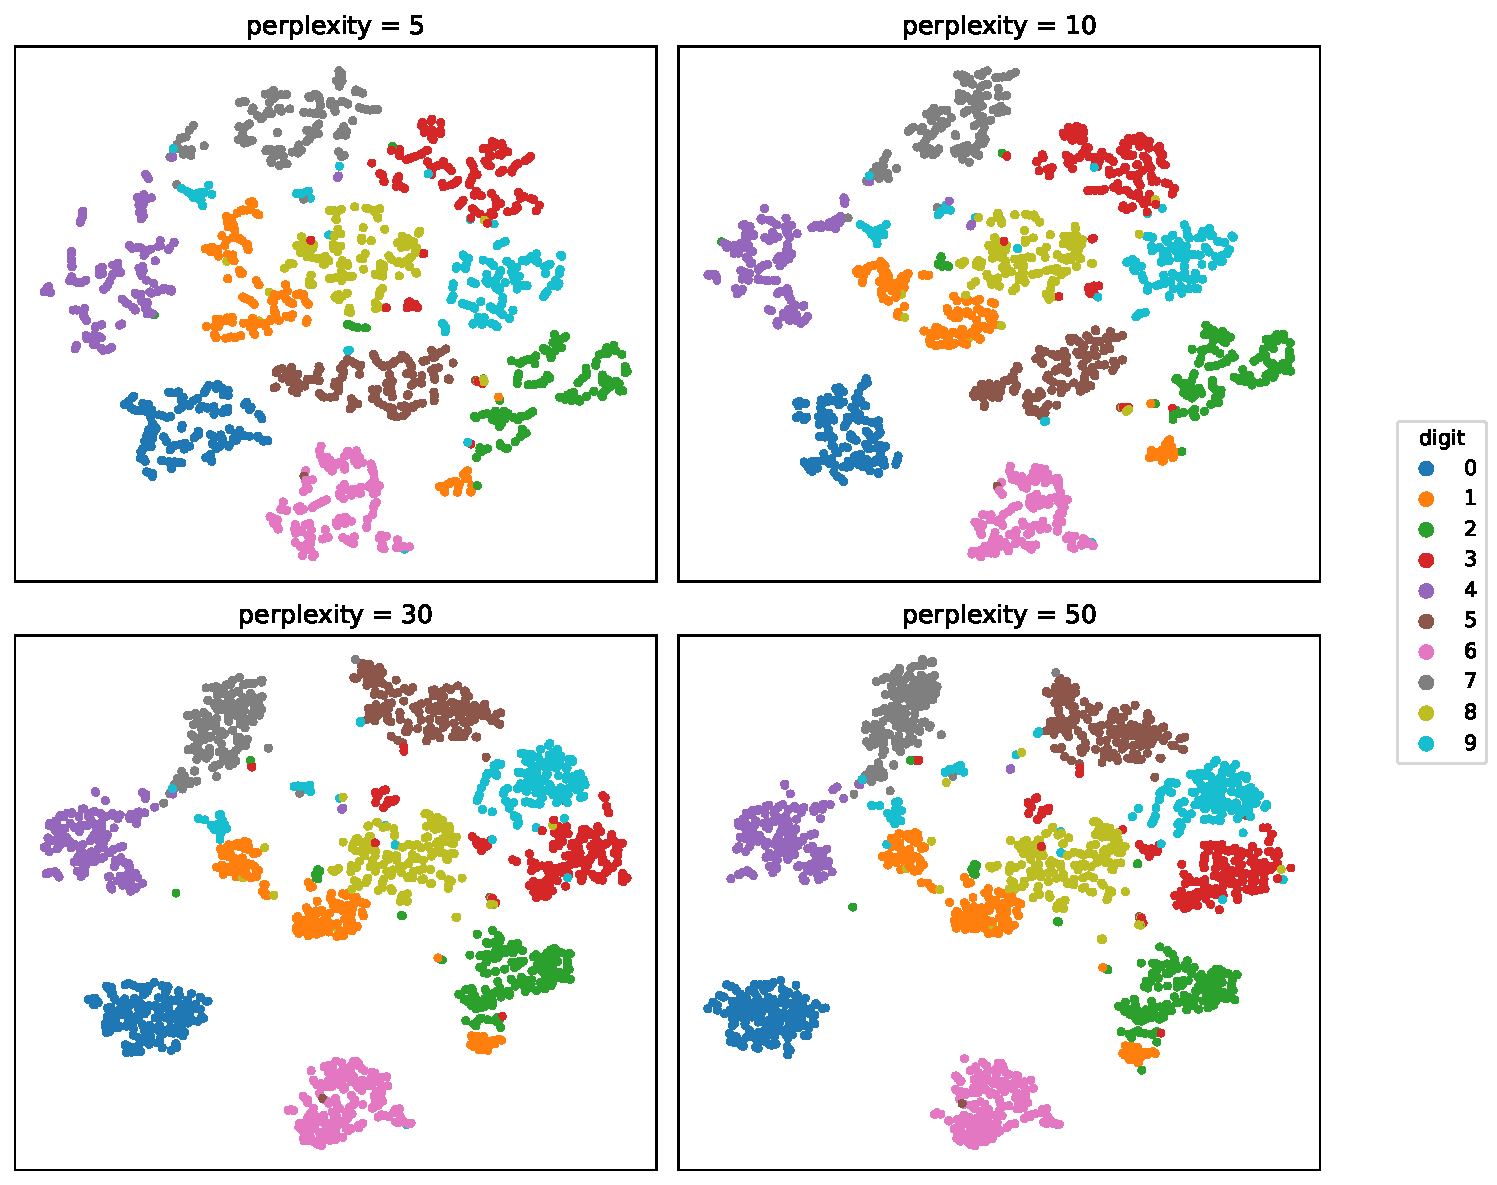
\includegraphics[keepaspectratio]{contents/3/embedding_files/figure-pdf/cell-8-output-1.pdf}}

The figure illustrates how \texttt{perplexity} changes the neighborhood
scale used by t-SNE. Smaller values emphasize fine local structure,
often producing many tight or fragmented clusters. Larger values
consider broader neighborhoods, leading to smoother and more stable
embeddings.

Some observations from the plots are:

\begin{itemize}
\tightlist
\item
  All \texttt{perplexity} values separate most digit classes, indicating
  that the handwritten digits have meaningful local neighborhood
  structure in the original high-dimensional space.
\item
  With small \texttt{perplexity} (5--10), the embedding focuses on very
  local neighborhoods. Clusters are more fragmented, and some digit
  classes appear as multiple disconnected regions. This suggests that
  some digit classes contain multiple local neighborhoods in the
  original feature space, although these disconnected regions should not
  automatically be interpreted as genuine subtypes.
\item
  In this example, increasing \texttt{perplexity} (30--50) produces more
  compact and stable clusters. Samples from the same digit are grouped
  more consistently, resulting in a cleaner overall layout.
\item
  The embeddings for \texttt{perplexity} 30 and 50 are visually similar,
  suggesting that the recovered local neighborhood structure is
  relatively stable over this range.
\item
  Some overlap between visually similar digits persists under all
  settings, possibly reflecting genuine ambiguity in the handwritten
  digits rather than an inappropriate choice of \texttt{perplexity}.
\item
  Although local neighborhoods are largely preserved, the relative
  positions, sizes, and distances between clusters change noticeably
  across \texttt{perplexity} values. Therefore, these global geometric
  relationships should not be interpreted quantitatively.
\end{itemize}

Overall, \texttt{perplexity} controls the trade-off between emphasizing
fine local neighborhoods and producing a smoother representation of the
underlying neighborhood structure, rather than determining the number of
clusters.

A useful \texttt{perplexity} is one that produces stable local
neighborhoods across a reasonable range of parameter values rather than
one that gives the most visually appealing plot. Comparing several
\texttt{perplexity} values is therefore often more informative than
selecting a single ``best'' visualization. When class labels are
available, they should be used only after fitting to verify whether
nearby points correspond to similar observations. The embedding can then
guide further exploration of the original data. For example, overlapping
digit classes can be examined in the original images to determine
whether the ambiguity reflects genuine variation in handwriting rather
than an artifact of the visualization.

\section{UMAP}\label{umap}

UMAP stands for Uniform Manifold Approximation and Projection. Like
t-SNE, it is a nonlinear embedding method based on local neighborhoods
and is often used for two-dimensional visualization. The main difference
is that UMAP builds a weighted nearest-neighbor graph in the original
space and then tries to reproduce that graph in a low-dimensional
display.

Unlike standard \texttt{sklearn} t-SNE, the common Python implementation
of UMAP can also transform new observations after fitting. This makes
UMAP somewhat easier to reuse in a later workflow, although the first
purpose here is still visualization and diagnosis.

The main idea is:

\[
X
\longrightarrow
\text{high-dimensional nearest-neighbor graph } W
\longrightarrow
\text{low-dimensional coordinates with a similar graph}.
\]

\subsection{Mathematical Idea}\label{mathematical-idea-2}

The core algorithm is similar in spirit to t-SNE:

\begin{enumerate}
\def\labelenumi{\arabic{enumi}.}
\tightlist
\item
  For each observation, find its nearest neighbors in the original
  space.
\item
  Turn these local neighborhoods into a weighted graph \(W=(w_{ij})\). A
  larger \(w_{ij}\) means that observations \(i\) and \(j\) are strongly
  connected in the original representation.
\item
  Introduce low-dimensional coordinates \(z_1,\ldots,z_n\).
\item
  From the distances among the \(z_i\)'s, build a low-dimensional graph
  \(R(Z)=(r_{ij})\).
\item
  Move the \(z_i\)'s so that the low-dimensional graph resembles the
  original graph.
\end{enumerate}

In other words, UMAP chooses the plotted coordinates by minimizing a
graph cross-entropy loss between the original graph \(W\) and the
low-dimensional graph \(R(Z)\):

\[
\min_{z_1,\ldots,z_n}
\operatorname{CE}\qty(W, R(Z)).
\]

Thus UMAP does not try to reconstruct the original features. It tries to
preserve a local nearest-neighbor graph. The details use fuzzy-set
language, but the practical interpretation is simple: observations that
are strongly connected in the original graph should stay close in the
display, while weakly connected observations may be placed farther
apart.

\begin{tcolorbox}[enhanced jigsaw, arc=.35mm, bottomrule=.15mm, bottomtitle=1mm, breakable, colback=white, colbacktitle=quarto-callout-note-color!10!white, colframe=quarto-callout-note-color-frame, coltitle=black, left=2mm, leftrule=.75mm, opacityback=0, opacitybacktitle=0.6, rightrule=.15mm, title=\textcolor{quarto-callout-note-color}{\faInfo}\hspace{0.5em}{How UMAP builds \(W\)}, titlerule=0mm, toprule=.15mm, toptitle=1mm]

UMAP first finds the nearest neighbors of each observation according to
the chosen distance metric. The parameter \texttt{n\_neighbors} controls
the size of these local neighborhoods. For each point \(x_i\), UMAP uses
only its selected nearest neighbors as candidate directed edges from
\(i\). Points outside this selected neighbor set usually have directed
weight \(a_{ij}=0\) from the point of view of \(i\).

After the candidate neighbors are selected, UMAP assigns a local
distance offset \(\rho_i\) and a local scale \(\sigma_i\) for each
point. The offset \(\rho_i\) is usually the distance from \(x_i\) to its
nearest neighbor. This makes the nearest neighbor receive weight \(1\).
The scale \(\sigma_i\) controls how quickly the remaining selected
neighbors lose weight as distance increases. Both \(\rho_i\) and
\(\sigma_i\) are chosen automatically by the algorithm for each point;
they are not tuning parameters set by the user.

A simplified version of the directed neighbor weight from \(i\) to \(j\)
is

\[
a_{ij}
=
\exp\qty(
-\frac{\max\{0,d(x_i,x_j)-\rho_i\}}{\sigma_i}
).
\]

Thus the construction is

\[
\texttt{n\_neighbors}
\longrightarrow
\text{selected neighbor set}
\longrightarrow
(\rho_i,\sigma_i)
\longrightarrow
a_{ij}
\longrightarrow
W.
\]

The parameter \texttt{n\_neighbors} decides which points are considered
local neighbors. The parameters \(\rho_i\) and \(\sigma_i\) then decide
how strongly those selected neighbors are connected. Thus UMAP, like
t-SNE, uses local distance scales instead of one global bandwidth for
the whole dataset.

The formula has a simple piecewise interpretation. If \(x_j\) is within
the local offset of \(x_i\), so that

\[
d(x_i,x_j)\le \rho_i,
\]

then \(\max\{0,d(x_i,x_j)-\rho_i\}=0\) and therefore
\(a_{ij}=\exp(0)=1\). If \(x_j\) is farther away than \(\rho_i\), then

\[
a_{ij}
=
\exp\qty(
-\frac{d(x_i,x_j)-\rho_i}{\sigma_i}
),
\]

so the directed connection strength decays exponentially with distance.
For the directed weights \(a_{ij}\), the nearest neighbor has weight
approximately \(1\), selected but farther neighbors receive exponential
weights between \(0\) and \(1\), and points outside the selected
\texttt{n\_neighbors} set have weight \(0\) from \(i\) to \(j\).

The directed weights are then combined into a symmetric graph:

\[
w_{ij}
=
a_{ij}+a_{ji}-a_{ij}a_{ji}.
\]

This produces the high-dimensional graph \(W=(w_{ij})\). Formally, \(W\)
is an \(n\times n\) weighted adjacency matrix: \(w_{ij}\) measures the
strength of the local connection between observations \(i\) and \(j\) in
the original space. It is not a distance matrix. Larger \(w_{ij}\) means
a stronger neighbor relationship, and most entries are zero or very
small because UMAP is based on nearest neighbors.

The final weight \(w_{ij}\) is symmetric, so it combines both
directions. Even if \(x_j\) is not selected as a neighbor of \(x_i\),
the final \(w_{ij}\) can still be positive if \(x_i\) is selected as a
neighbor of \(x_j\).

\end{tcolorbox}

\begin{tcolorbox}[enhanced jigsaw, arc=.35mm, bottomrule=.15mm, bottomtitle=1mm, breakable, colback=white, colbacktitle=quarto-callout-note-color!10!white, colframe=quarto-callout-note-color-frame, coltitle=black, left=2mm, leftrule=.75mm, opacityback=0, opacitybacktitle=0.6, rightrule=.15mm, title=\textcolor{quarto-callout-note-color}{\faInfo}\hspace{0.5em}{How UMAP builds \(R(Z)\) and the cross-entropy}, titlerule=0mm, toprule=.15mm, toptitle=1mm]

After low-dimensional coordinates \(z_1,\ldots,z_n\) are introduced,
UMAP defines a low-dimensional graph \(R(Z)=(r_{ij})\) from pairwise
distances in the plot. A common form is

\[
r_{ij}
=
\frac{1}{1+\alpha\norm{z_i-z_j}^{2\beta}},
\]

Here \(\alpha\) and \(\beta\) are not usually chosen directly by the
user. They are fitted internally from UMAP's display parameters,
especially \texttt{min\_dist}. If two plotted points are close,
\(r_{ij}\) is large; if they are far apart, \(r_{ij}\) is small.

UMAP then moves the coordinates so that \(R(Z)\) resembles \(W\). This
is done by minimizing a cross-entropy loss of the form

\[
\operatorname{CE}(W,R)
=
-\sum_{i\ne j}
\left[
w_{ij}\log r_{ij}
+
(1-w_{ij})\log(1-r_{ij})
\right].
\]

The first term encourages pairs with large \(w_{ij}\) to stay close in
the plot. The second term discourages weakly connected pairs from all
collapsing into the same place. In practice, UMAP optimizes the
low-dimensional coordinates by stochastic gradient descent: sampled
edges from \(W\) pull connected points together, while randomly sampled
non-edges push unrelated points apart.

\end{tcolorbox}

\begin{tcolorbox}[enhanced jigsaw, arc=.35mm, bottomrule=.15mm, bottomtitle=1mm, breakable, colback=white, colbacktitle=quarto-callout-note-color!10!white, colframe=quarto-callout-note-color-frame, coltitle=black, left=2mm, leftrule=.75mm, opacityback=0, opacitybacktitle=0.6, rightrule=.15mm, title=\textcolor{quarto-callout-note-color}{\faInfo}\hspace{0.5em}{What \texttt{min\_dist} controls}, titlerule=0mm, toprule=.15mm, toptitle=1mm]

The parameter \texttt{min\_dist} is the effective minimum distance
between nearby points in the low-dimensional embedding. It is not a hard
constraint that all plotted points must be at least this far apart.
Instead, it defines the distance scale at which the low-dimensional
similarity should begin to decay.

UMAP does not usually ask the user to choose \(\alpha\) and \(\beta\)
directly. Instead, it fits \(\alpha\) and \(\beta\) from
\texttt{min\_dist} so that

\[
\frac{1}{1+\alpha d^{2\beta}}
\]

has a shape similar to a target curve: the curve stays near \(1\) for
distances below \texttt{min\_dist}, then decreases after that. Thus the
tuning chain is

\[
\texttt{min\_dist}
\longrightarrow
(\alpha,\beta)
\longrightarrow
r_{ij}
=
\frac{1}{1+\alpha\norm{z_i-z_j}^{2\beta}}
\longrightarrow
R(Z).
\]

The practical interpretation is:

\begin{itemize}
\tightlist
\item
  \texttt{min\_dist} does not define the original nearest-neighbor graph
  \(W\). That graph is mainly determined by \texttt{metric} and
  \texttt{n\_neighbors}.
\item
  \texttt{min\_dist} affects the low-dimensional graph \(R(Z)\) through
  the fitted values of \(\alpha\) and \(\beta\).
\item
  Smaller \texttt{min\_dist} allows points that are strongly connected
  in \(W\) to be placed closer together in the low-dimensional
  embedding. This usually produces tighter visual clusters.
\item
  Larger \texttt{min\_dist} keeps strongly connected points more spread
  out. This can make continuous structure and within-group variation
  easier to see, but the plot may look less clustered.
\item
  A tight island in a UMAP plot does not automatically mean that the
  original data have high density there. It may simply reflect a small
  \texttt{min\_dist}.
\end{itemize}

\end{tcolorbox}

\subsection{What structure does UMAP
preserve?}\label{what-structure-does-umap-preserve}

UMAP preserves local nearest-neighbor graph structure, not the original
coordinates, not the original feature meanings, and not exact Euclidean
distances. The input graph depends on the chosen distance metric and on
the neighborhood size \texttt{n\_neighbors}. These determine the
original graph \(W\) that UMAP tries to preserve. The parameter
\texttt{min\_dist} does not change \(W\); it changes how tightly
connected points may be packed in the low-dimensional display.

In plain language:

\begin{itemize}
\tightlist
\item
  If two observations are nearest neighbors in the original
  representation, UMAP tries to keep them close or connected in the
  plot.
\item
  If two groups are connected by many nearest-neighbor edges, UMAP may
  place them near each other even if the original geometry is curved or
  nonlinear.
\item
  Distances between faraway islands, island sizes, axis directions, and
  visual densities should not be treated as exact quantitative
  information.
\item
  Compared with t-SNE, UMAP often keeps a little more broad structure,
  but this depends strongly on \texttt{n\_neighbors} and should still be
  checked.
\end{itemize}

\begin{tcolorbox}[enhanced jigsaw, arc=.35mm, bottomrule=.15mm, bottomtitle=1mm, breakable, colback=white, colbacktitle=quarto-callout-note-color!10!white, colframe=quarto-callout-note-color-frame, coltitle=black, left=2mm, leftrule=.75mm, opacityback=0, opacitybacktitle=0.6, rightrule=.15mm, title=\textcolor{quarto-callout-note-color}{\faInfo}\hspace{0.5em}{UMAP as a diagnostic plot}, titlerule=0mm, toprule=.15mm, toptitle=1mm]

UMAP is useful when we want to inspect whether local nearest-neighbor
relationships reveal structure that a linear plot such as PCA misses.
Like t-SNE, it is mainly a visualization and diagnostic tool: visible
groups are hypotheses to investigate, not automatic cluster definitions.

UMAP can also be useful after clustering. If cluster labels form
coherent local regions in a UMAP plot, then the clustering is consistent
with the nearest-neighbor graph shown by UMAP. If labels are heavily
mixed, the clustering may not match local structure, or the data may not
contain clearly separated groups. Formal evaluation should still use
criteria tied to the analysis goal, such as nearest-neighbor overlap,
silhouette score, or adjusted Rand index when labels are available.

\end{tcolorbox}

\subsection{UMAP in Python}\label{umap-in-python}

The standard implementation is provided by \texttt{umap-learn}. If it is
not installed, you may install it directly.

\begin{Shaded}
\begin{Highlighting}[]
\ExtensionTok{uv}\NormalTok{ add umap{-}learn}
\end{Highlighting}
\end{Shaded}

We use the same standardized digits data and the same 30-dimensional PCA
preprocessing as in the t-SNE example.

\begin{Shaded}
\begin{Highlighting}[]
\ImportTok{import}\NormalTok{ umap}

\NormalTok{umap\_model }\OperatorTok{=}\NormalTok{ umap.UMAP(}
\NormalTok{    n\_neighbors}\OperatorTok{=}\DecValTok{15}\NormalTok{,}
\NormalTok{    min\_dist}\OperatorTok{=}\FloatTok{0.1}\NormalTok{,}
\NormalTok{    n\_components}\OperatorTok{=}\DecValTok{2}\NormalTok{,}
\NormalTok{    metric}\OperatorTok{=}\StringTok{"euclidean"}\NormalTok{,}
\NormalTok{    random\_state}\OperatorTok{=}\DecValTok{1}\NormalTok{,}
\NormalTok{)}

\NormalTok{Z\_umap }\OperatorTok{=}\NormalTok{ umap\_model.fit\_transform(X\_digits\_pca)}
\end{Highlighting}
\end{Shaded}

In this example, \texttt{n\_neighbors=15} sets a moderate local
neighborhood size, and \texttt{min\_dist=0.1} allows fairly compact
visual groups. These are tuning choices, not universal defaults.

\begin{itemize}
\tightlist
\item
  The parameter \texttt{n\_neighbors} controls the construction of the
  high-dimensional graph \(W\): it determines how many nearby
  observations each point uses when UMAP builds the weighted
  nearest-neighbor graph. A small value, such as \texttt{5} or
  \texttt{10}, makes UMAP focus on very local neighborhoods. This can
  reveal fine structure, but it can also break continuous structure into
  many small islands. A larger value, such as \texttt{30} or
  \texttt{50}, asks UMAP to use broader neighborhoods. This often gives
  a smoother layout and may preserve more large-scale relationships, but
  it can hide small local differences.
\item
  The parameter \texttt{metric} defines distance in the original feature
  space, so it determines which observations count as nearest neighbors
  before UMAP does any embedding. For standardized numeric features,
  \texttt{"euclidean"} is a common starting point. For sparse counts or
  text-like features, cosine distance is often more appropriate.
  Changing \texttt{metric} can change the graph \(W\) itself, so it can
  change the embedding more fundamentally than changing only the visual
  display parameters.
\item
  The parameter \texttt{min\_dist} affects the low-dimensional graph
  \(R(Z)\) rather than the original graph \(W\). Smaller values allow
  tighter visual groups, while larger values keep connected points more
  spread out. In practice, try several combinations of
  \texttt{n\_neighbors} and \texttt{min\_dist}. Patterns that remain
  visible across reasonable settings are more credible than patterns
  that appear only under one parameter choice.
\end{itemize}

\begin{tcolorbox}[enhanced jigsaw, arc=.35mm, bottomrule=.15mm, bottomtitle=1mm, breakable, colback=white, colbacktitle=quarto-callout-note-color!10!white, colframe=quarto-callout-note-color-frame, coltitle=black, left=2mm, leftrule=.75mm, opacityback=0, opacitybacktitle=0.6, rightrule=.15mm, title=\textcolor{quarto-callout-note-color}{\faInfo}\hspace{0.5em}{Initialization in UMAP}, titlerule=0mm, toprule=.15mm, toptitle=1mm]

UMAP can use PCA initialization, but it usually does not rely on it.
Since UMAP first builds a nearest-neighbor graph \(W\), the default
initialization is typically graph-based, using spectral initialization
from that graph. PCA initialization is possible, but it is not the
central idea.

\end{tcolorbox}

We plot the result from the above code.

\begin{Shaded}
\begin{Highlighting}[]
\NormalTok{fig, ax }\OperatorTok{=}\NormalTok{ plt.subplots(figsize}\OperatorTok{=}\NormalTok{(}\DecValTok{8}\NormalTok{, }\DecValTok{6}\NormalTok{))}
\NormalTok{scatter }\OperatorTok{=}\NormalTok{ ax.scatter(}
\NormalTok{    Z\_umap[:, }\DecValTok{0}\NormalTok{],}
\NormalTok{    Z\_umap[:, }\DecValTok{1}\NormalTok{],}
\NormalTok{    c}\OperatorTok{=}\NormalTok{y\_digits,}
\NormalTok{    cmap}\OperatorTok{=}\StringTok{"tab10"}\NormalTok{,}
\NormalTok{    s}\OperatorTok{=}\DecValTok{10}\NormalTok{,}
\NormalTok{    alpha}\OperatorTok{=}\FloatTok{0.75}\NormalTok{,}
\NormalTok{)}
\NormalTok{ax.set\_xlabel(}\StringTok{"UMAP1"}\NormalTok{)}
\NormalTok{ax.set\_ylabel(}\StringTok{"UMAP2"}\NormalTok{)}
\NormalTok{ax.set\_title(}\StringTok{"Digits UMAP"}\NormalTok{)}
\NormalTok{ax.legend(}\OperatorTok{*}\NormalTok{scatter.legend\_elements(), title}\OperatorTok{=}\StringTok{"digit"}\NormalTok{, ncol}\OperatorTok{=}\DecValTok{2}\NormalTok{)}\OperatorTok{;}
\end{Highlighting}
\end{Shaded}

\pandocbounded{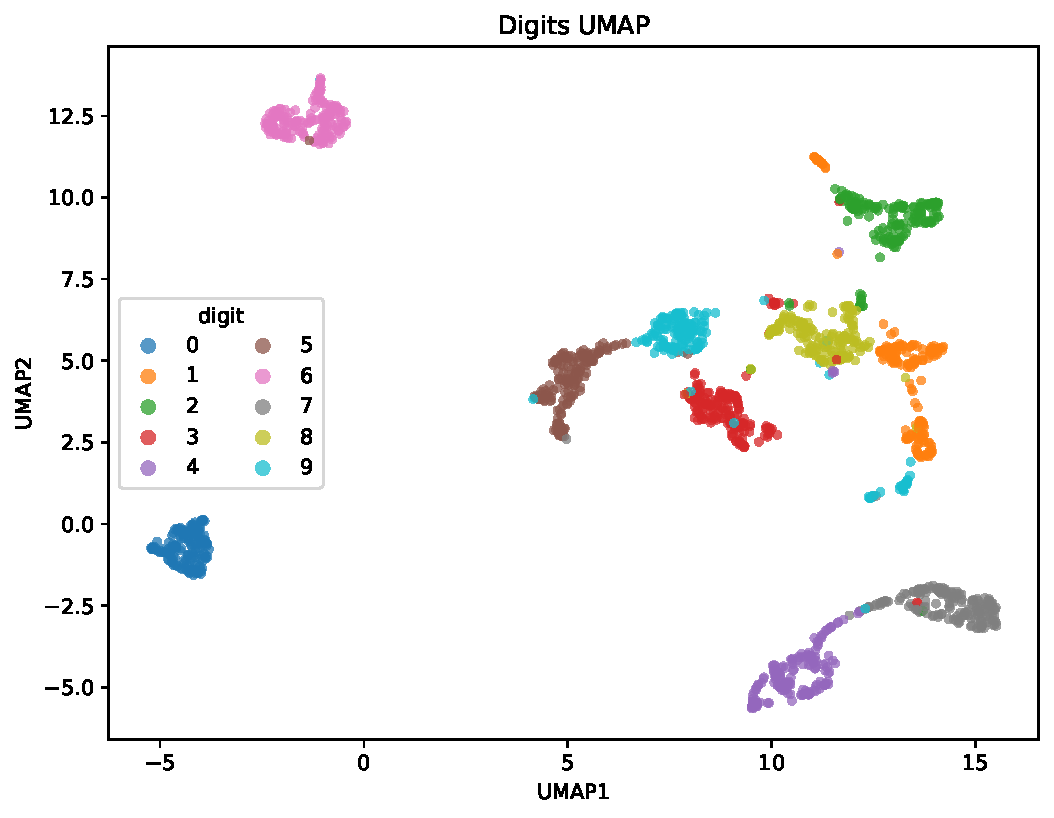
\includegraphics[keepaspectratio]{contents/3/embedding_files/figure-pdf/cell-10-output-1.pdf}}

We will try different combinations of \texttt{n\_neighbors} and
\texttt{min\_dist}.

\begin{Shaded}
\begin{Highlighting}[]
\NormalTok{n\_neighbors\_values }\OperatorTok{=}\NormalTok{ [}\DecValTok{5}\NormalTok{, }\DecValTok{15}\NormalTok{, }\DecValTok{50}\NormalTok{]}
\NormalTok{min\_dist\_values }\OperatorTok{=}\NormalTok{ [}\FloatTok{0.05}\NormalTok{, }\FloatTok{0.10}\NormalTok{, }\FloatTok{0.50}\NormalTok{]}

\NormalTok{fig, axs }\OperatorTok{=}\NormalTok{ plt.subplots(}\DecValTok{3}\NormalTok{, }\DecValTok{3}\NormalTok{, figsize}\OperatorTok{=}\NormalTok{(}\DecValTok{12}\NormalTok{, }\DecValTok{10}\NormalTok{))}
\NormalTok{scatter }\OperatorTok{=} \VariableTok{None}

\ControlFlowTok{for}\NormalTok{ row, n\_neighbors }\KeywordTok{in} \BuiltInTok{enumerate}\NormalTok{(n\_neighbors\_values):}
    \ControlFlowTok{for}\NormalTok{ col, min\_dist }\KeywordTok{in} \BuiltInTok{enumerate}\NormalTok{(min\_dist\_values):}
\NormalTok{        ax }\OperatorTok{=}\NormalTok{ axs[row, col]}
\NormalTok{        model }\OperatorTok{=}\NormalTok{ umap.UMAP(}
\NormalTok{            n\_neighbors}\OperatorTok{=}\NormalTok{n\_neighbors,}
\NormalTok{            min\_dist}\OperatorTok{=}\NormalTok{min\_dist,}
\NormalTok{            random\_state}\OperatorTok{=}\DecValTok{1}\NormalTok{,}
\NormalTok{        )}
\NormalTok{        embedding }\OperatorTok{=}\NormalTok{ model.fit\_transform(X\_digits\_pca)}
\NormalTok{        scatter }\OperatorTok{=}\NormalTok{ ax.scatter(}
\NormalTok{            embedding[:, }\DecValTok{0}\NormalTok{],}
\NormalTok{            embedding[:, }\DecValTok{1}\NormalTok{],}
\NormalTok{            c}\OperatorTok{=}\NormalTok{y\_digits,}
\NormalTok{            cmap}\OperatorTok{=}\StringTok{"tab10"}\NormalTok{,}
\NormalTok{            s}\OperatorTok{=}\DecValTok{6}\NormalTok{,}
\NormalTok{        )}
\NormalTok{        ax.set\_title(}\SpecialStringTok{f"n\_neighbors=}\SpecialCharTok{\{}\NormalTok{n\_neighbors}\SpecialCharTok{\}}\SpecialStringTok{, min\_dist=}\SpecialCharTok{\{}\NormalTok{min\_dist}\SpecialCharTok{\}}\SpecialStringTok{"}\NormalTok{)}
\NormalTok{        ax.set\_xticks([])}
\NormalTok{        ax.set\_yticks([])}

\NormalTok{fig.legend(}
    \OperatorTok{*}\NormalTok{scatter.legend\_elements(),}
\NormalTok{    title}\OperatorTok{=}\StringTok{"digit"}\NormalTok{,}
\NormalTok{    loc}\OperatorTok{=}\StringTok{"center right"}\NormalTok{,}
\NormalTok{)}
\NormalTok{fig.tight\_layout(rect}\OperatorTok{=}\NormalTok{[}\DecValTok{0}\NormalTok{, }\DecValTok{0}\NormalTok{, }\FloatTok{0.9}\NormalTok{, }\DecValTok{1}\NormalTok{])}\OperatorTok{;}
\end{Highlighting}
\end{Shaded}

\pandocbounded{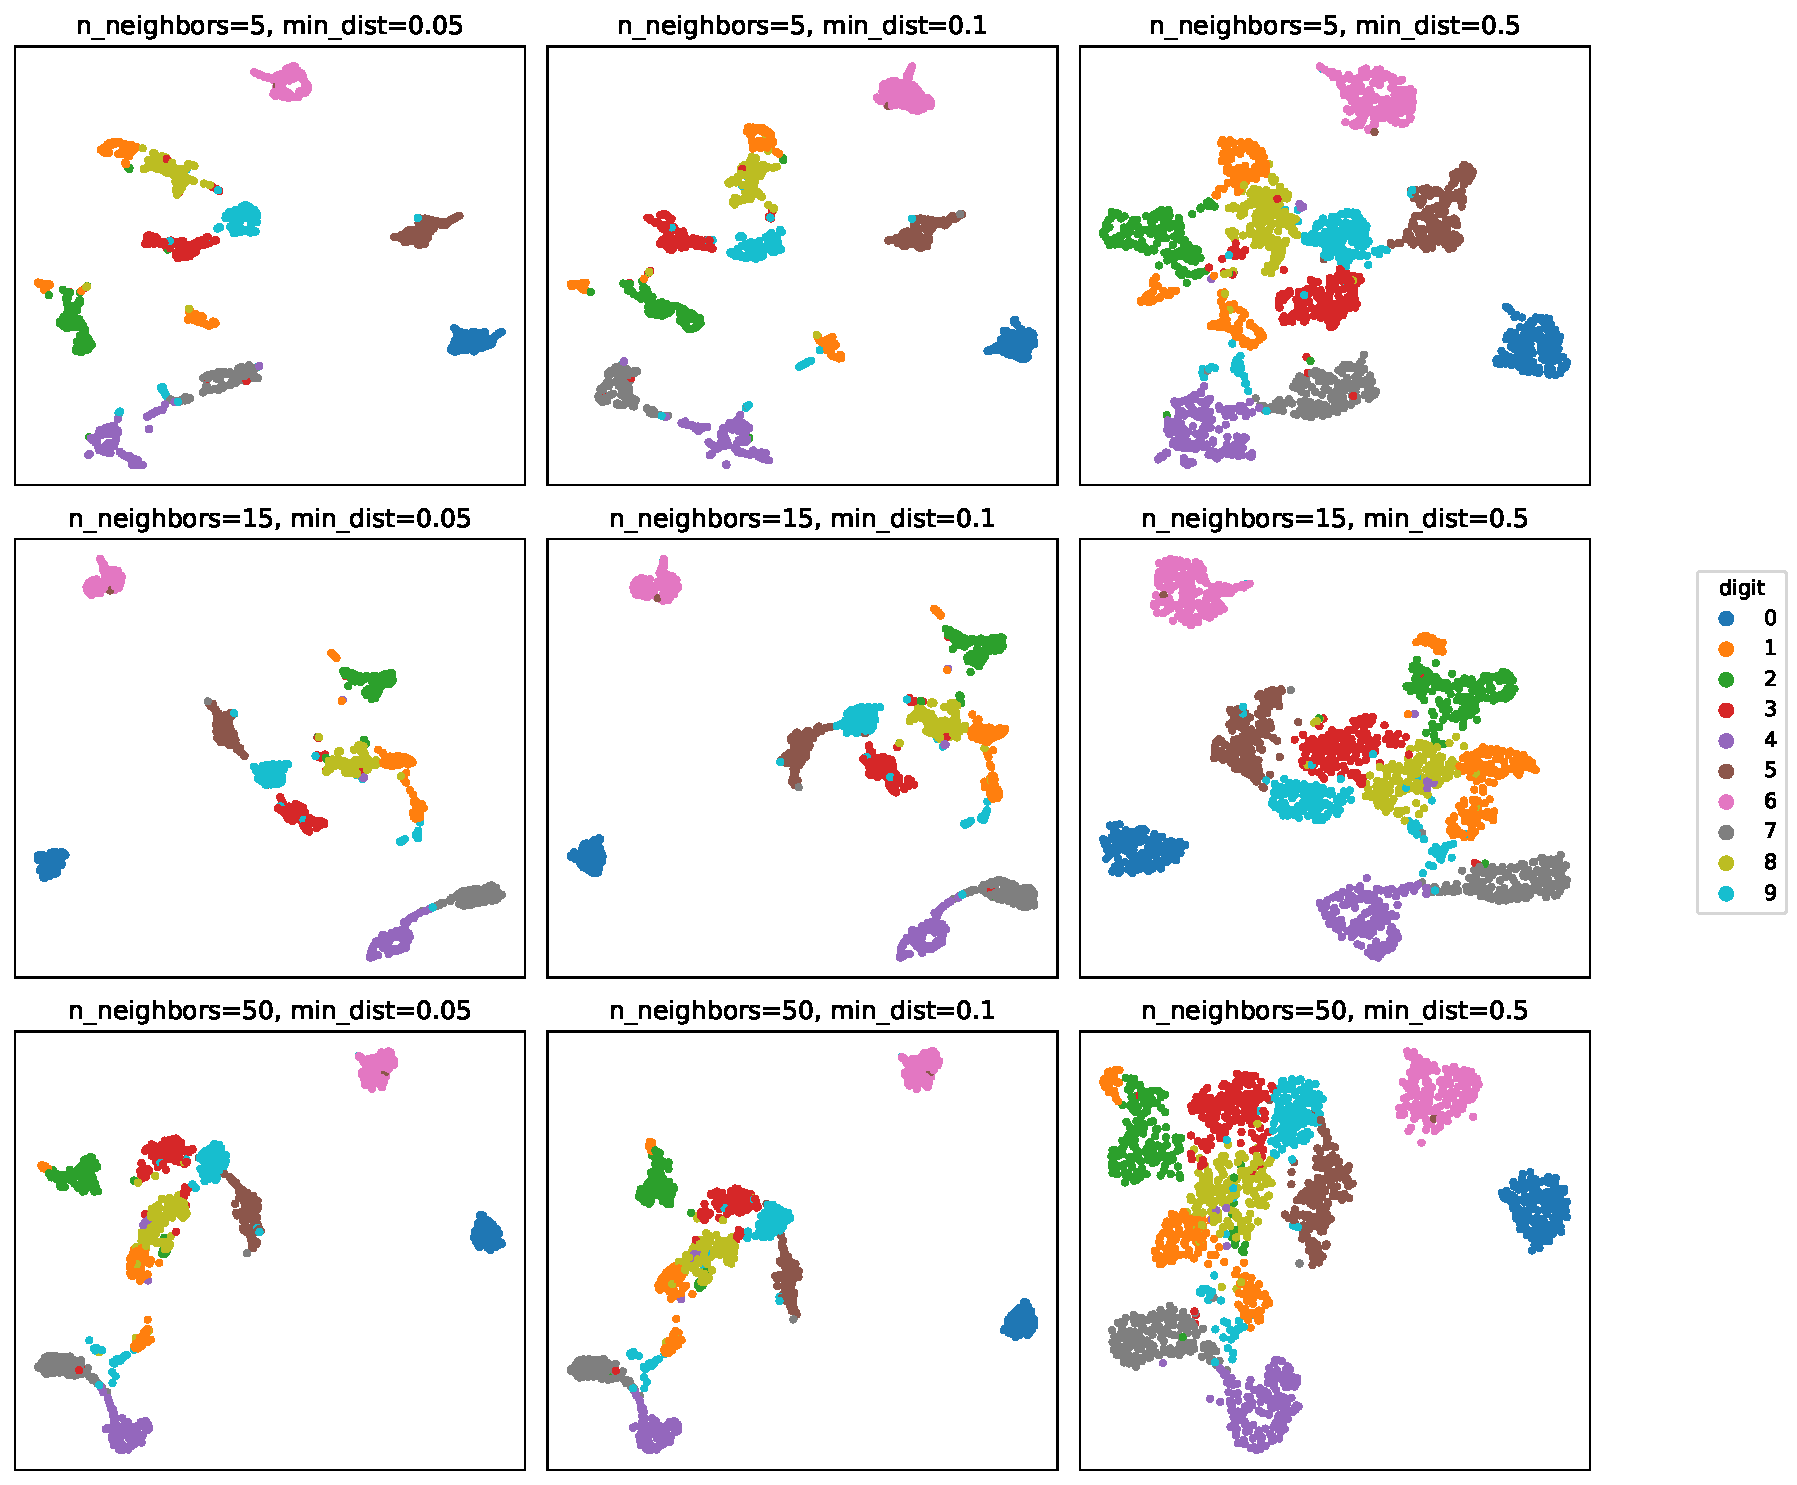
\includegraphics[keepaspectratio]{contents/3/embedding_files/figure-pdf/cell-11-output-1.pdf}}

Some observations from the plots are:

\begin{itemize}
\tightlist
\item
  The overall class structure is relatively stable across all parameter
  settings. Most digit classes remain recognizable, indicating that the
  underlying local neighborhood structure is robust.
\item
  Digits \texttt{0} and \texttt{6} remain well separated from most other
  classes in all embeddings, suggesting that these digits have
  distinctive local pixel patterns.
\item
  Several groups of digits remain in neighboring regions across
  different parameter settings, although their relative positions change
  as the hyperparameters vary.
\item
  Some digit classes appear as multiple disconnected regions when
  \texttt{n\_neighbors} is small. This suggests that the class may
  contain several distinct local neighborhoods in the original feature
  space, although these should not automatically be interpreted as true
  subtypes.
\item
  Increasing \texttt{min\_dist} primarily changes the compactness of the
  embedding. Smaller values produce tighter clusters, whereas larger
  values spread nearby points farther apart.
\item
  Increasing \texttt{n\_neighbors} generally produces a smoother and
  more stable overall layout by incorporating broader neighborhood
  information during graph construction.
\item
  Although the global layout changes noticeably across parameter
  settings, the major local neighborhoods remain largely consistent.
\end{itemize}

These patterns can also guide inspection of the original data. For
example, if several digit classes remain connected or neighboring in the
UMAP plot, we can examine those images to understand which strokes or
handwriting styles make the classes similar.

\section{Comparing the Methods}\label{comparing-the-methods}

The unsupervised methods in this chapter and the previous chapter are
related because they all produce lower-dimensional representations of
high-dimensional data. For that reason, they may appear to be
interchangeable: PCA, spectral embedding, t-SNE, and UMAP can all be
used to make a two-dimensional plot.

However, they are not trying to preserve the same structure. PCA
preserves linear variance. Spectral embedding preserves connectivity in
a chosen graph. t-SNE attempts to preserve neighborhood probabilities.
UMAP attempts to preserve the weighted nearest-neighbor graph structure.
Therefore, the right method depends on the question we want the
visualization to answer.

This section compares the methods in two steps. First, we compare t-SNE
and UMAP directly, since both are nonlinear visualization methods based
on local neighborhoods. Then we compare all four methods together to
show how linear variance, graph connectivity, local neighbor
probabilities, and nearest-neighbor graph structure lead to different
visual conclusions.

\subsection{t-SNE vs UMAP}\label{t-sne-vs-umap}

t-SNE and UMAP are both nonlinear visualization methods based on local
relationships. They both start from high-dimensional distances, but they
preserve different objects.

For t-SNE, distances are converted into neighbor probabilities. The
high-dimensional probability distribution is \(P=(p_{ij})\), the
low-dimensional probability distribution is \(Q=(q_{ij})\), and t-SNE
moves the plotted points so that \(Q\) matches \(P\). The main tuning
parameter is \texttt{perplexity}, which controls the effective
neighborhood size used to construct \(P\).

For UMAP, distances are converted into a weighted nearest-neighbor
graph. The high-dimensional graph is \(W=(w_{ij})\), the low-dimensional
graph is \(R(Z)=(r_{ij})\), and UMAP moves the plotted points so that
\(R(Z)\) resembles \(W\). The parameter \texttt{n\_neighbors} controls
the neighborhood scale used to build \(W\), while \texttt{min\_dist}
controls how tightly connected points may be packed in the display.

This difference affects how we read the plots. In a t-SNE plot, a
continuous bridge made of many nearby points is meaningful: it suggests
that the original data may contain a chain of local neighbor
relationships connecting the two regions. But a large empty distance
between two t-SNE islands should not be interpreted as a reliable
measurement of how far apart the groups are in the original space. UMAP
has a more direct graph interpretation: connected regions in the plot
often reflect connections in the nearest-neighbor graph \(W\), although
that graph still depends on the chosen \texttt{metric} and
\texttt{n\_neighbors}.

So t-SNE is especially useful for inspecting very local neighborhoods.
UMAP is especially useful for inspecting nearest-neighbor graph
structure, comparing neighborhood scales, and sometimes reusing a fitted
embedding for new observations. Neither method should be used to make
strict claims about global distances, island sizes, densities, or axis
meanings.

\subsubsection{MNIST}\label{mnist}

We compare the methods on the famous
\href{https://www.openml.org/search?type=data&sort=runs&id=554}{MNIST
handwritten digit} dataset. MNIST has 70,000 images, and each image is
represented by \(28\times 28=784\) pixel features. Since the original
data are 784-dimensional, we cannot directly visualize the original
feature space as a scatter plot. Instead, we first inspect a few raw
digit images, and then visualize two-dimensional embeddings.

We use \texttt{fetch\_openml("mnist\_784")} to load the dataset. For
speed, the embedding examples below use a fixed random subset of 3000
images.

\begin{Shaded}
\begin{Highlighting}[]
\ImportTok{from}\NormalTok{ sklearn.datasets }\ImportTok{import}\NormalTok{ fetch\_openml}
\ImportTok{from}\NormalTok{ sklearn.preprocessing }\ImportTok{import}\NormalTok{ StandardScaler}
\ImportTok{import}\NormalTok{ numpy }\ImportTok{as}\NormalTok{ np}

\NormalTok{mnist }\OperatorTok{=}\NormalTok{ fetch\_openml(}\StringTok{"mnist\_784"}\NormalTok{, version}\OperatorTok{=}\DecValTok{1}\NormalTok{, as\_frame}\OperatorTok{=}\VariableTok{False}\NormalTok{)}

\NormalTok{rng }\OperatorTok{=}\NormalTok{ np.random.default\_rng(}\DecValTok{1}\NormalTok{)}
\NormalTok{sample\_index }\OperatorTok{=}\NormalTok{ rng.choice(mnist.data.shape[}\DecValTok{0}\NormalTok{], size}\OperatorTok{=}\DecValTok{3000}\NormalTok{, replace}\OperatorTok{=}\VariableTok{False}\NormalTok{)}

\NormalTok{X\_mnist\_raw }\OperatorTok{=}\NormalTok{ mnist.data[sample\_index]}
\NormalTok{y\_mnist }\OperatorTok{=}\NormalTok{ mnist.target[sample\_index].astype(}\BuiltInTok{int}\NormalTok{)}

\NormalTok{X\_mnist }\OperatorTok{=}\NormalTok{ StandardScaler().fit\_transform(X\_mnist\_raw)}
\end{Highlighting}
\end{Shaded}

Here are some sample images from MNIST. As with the \texttt{digits}
dataset, we use \texttt{imshow()} to display each digit as a matrix of
pixel intensities.

\begin{Shaded}
\begin{Highlighting}[]
\ImportTok{import}\NormalTok{ matplotlib.pyplot }\ImportTok{as}\NormalTok{ plt}

\NormalTok{fig, axs }\OperatorTok{=}\NormalTok{ plt.subplots(}\DecValTok{2}\NormalTok{, }\DecValTok{5}\NormalTok{, figsize}\OperatorTok{=}\NormalTok{(}\DecValTok{7}\NormalTok{, }\DecValTok{3}\NormalTok{))}

\ControlFlowTok{for}\NormalTok{ ax, digit }\KeywordTok{in} \BuiltInTok{zip}\NormalTok{(axs.ravel(), }\BuiltInTok{range}\NormalTok{(}\DecValTok{10}\NormalTok{)):}
\NormalTok{    image }\OperatorTok{=}\NormalTok{ X\_mnist\_raw[y\_mnist }\OperatorTok{==}\NormalTok{ digit][}\DecValTok{0}\NormalTok{].reshape(}\DecValTok{28}\NormalTok{, }\DecValTok{28}\NormalTok{)}
\NormalTok{    ax.imshow(image, cmap}\OperatorTok{=}\StringTok{"gray\_r"}\NormalTok{)}
\NormalTok{    ax.set\_title(}\SpecialStringTok{f"digit }\SpecialCharTok{\{}\NormalTok{digit}\SpecialCharTok{\}}\SpecialStringTok{"}\NormalTok{)}
\NormalTok{    ax.axis(}\StringTok{"off"}\NormalTok{)}\OperatorTok{;}
\end{Highlighting}
\end{Shaded}

\pandocbounded{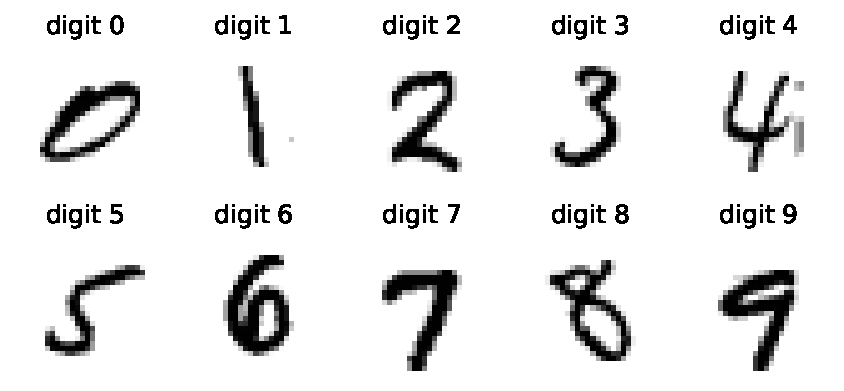
\includegraphics[keepaspectratio]{contents/3/embedding_files/figure-pdf/cell-13-output-1.pdf}}

Now we compare t-SNE and UMAP in two ways on this subset. The first row
uses the standardized 784-dimensional pixel features directly. The
second row first reduces the data to 50 principal components and then
applies t-SNE or UMAP. The colors are the digit labels, used only after
fitting to interpret the plots.

\begin{Shaded}
\begin{Highlighting}[]
\ImportTok{from}\NormalTok{ sklearn.manifold }\ImportTok{import}\NormalTok{ TSNE}
\ImportTok{from}\NormalTok{ sklearn.decomposition }\ImportTok{import}\NormalTok{ PCA}
\ImportTok{import}\NormalTok{ umap}

\NormalTok{X\_mnist\_pca50 }\OperatorTok{=}\NormalTok{ PCA(n\_components}\OperatorTok{=}\DecValTok{50}\NormalTok{, random\_state}\OperatorTok{=}\DecValTok{1}\NormalTok{).fit\_transform(X\_mnist)}

\NormalTok{Z\_tsne\_raw }\OperatorTok{=}\NormalTok{ TSNE(}
\NormalTok{    n\_components}\OperatorTok{=}\DecValTok{2}\NormalTok{, perplexity}\OperatorTok{=}\DecValTok{50}\NormalTok{, init}\OperatorTok{=}\StringTok{"pca"}\NormalTok{, learning\_rate}\OperatorTok{=}\StringTok{"auto"}\NormalTok{, random\_state}\OperatorTok{=}\DecValTok{1}
\NormalTok{).fit\_transform(X\_mnist)}

\NormalTok{Z\_umap\_raw }\OperatorTok{=}\NormalTok{ umap.UMAP(}
\NormalTok{    n\_components}\OperatorTok{=}\DecValTok{2}\NormalTok{, n\_neighbors}\OperatorTok{=}\DecValTok{15}\NormalTok{, min\_dist}\OperatorTok{=}\FloatTok{0.1}\NormalTok{, metric}\OperatorTok{=}\StringTok{"euclidean"}\NormalTok{, random\_state}\OperatorTok{=}\DecValTok{1}
\NormalTok{).fit\_transform(X\_mnist)}

\NormalTok{Z\_tsne\_compare }\OperatorTok{=}\NormalTok{ TSNE(}
\NormalTok{    n\_components}\OperatorTok{=}\DecValTok{2}\NormalTok{, perplexity}\OperatorTok{=}\DecValTok{50}\NormalTok{, init}\OperatorTok{=}\StringTok{"pca"}\NormalTok{, learning\_rate}\OperatorTok{=}\StringTok{"auto"}\NormalTok{, random\_state}\OperatorTok{=}\DecValTok{1}
\NormalTok{).fit\_transform(X\_mnist\_pca50)}

\NormalTok{Z\_umap\_compare }\OperatorTok{=}\NormalTok{ umap.UMAP(}
\NormalTok{    n\_components}\OperatorTok{=}\DecValTok{2}\NormalTok{, n\_neighbors}\OperatorTok{=}\DecValTok{15}\NormalTok{, min\_dist}\OperatorTok{=}\FloatTok{0.1}\NormalTok{, metric}\OperatorTok{=}\StringTok{"euclidean"}\NormalTok{, random\_state}\OperatorTok{=}\DecValTok{1}
\NormalTok{).fit\_transform(X\_mnist\_pca50)}

\NormalTok{embedding\_grid }\OperatorTok{=}\NormalTok{ \{}
    \StringTok{"Raw + t{-}SNE"}\NormalTok{: Z\_tsne\_raw,}
    \StringTok{"Raw + UMAP"}\NormalTok{: Z\_umap\_raw,}
    \StringTok{"PCA50 + t{-}SNE"}\NormalTok{: Z\_tsne\_compare,}
    \StringTok{"PCA50 + UMAP"}\NormalTok{: Z\_umap\_compare,}
\NormalTok{\}}

\NormalTok{fig, axs }\OperatorTok{=}\NormalTok{ plt.subplots(}\DecValTok{2}\NormalTok{, }\DecValTok{2}\NormalTok{, figsize}\OperatorTok{=}\NormalTok{(}\DecValTok{11}\NormalTok{, }\DecValTok{9}\NormalTok{))}

\NormalTok{scatter }\OperatorTok{=} \VariableTok{None}
\ControlFlowTok{for}\NormalTok{ ax, (name, Z\_method) }\KeywordTok{in} \BuiltInTok{zip}\NormalTok{(axs.ravel(), embedding\_grid.items()):}
\NormalTok{    scatter }\OperatorTok{=}\NormalTok{ ax.scatter(}
\NormalTok{        Z\_method[:, }\DecValTok{0}\NormalTok{], Z\_method[:, }\DecValTok{1}\NormalTok{], c}\OperatorTok{=}\NormalTok{y\_mnist, cmap}\OperatorTok{=}\StringTok{"tab10"}\NormalTok{, s}\OperatorTok{=}\DecValTok{10}\NormalTok{, alpha}\OperatorTok{=}\FloatTok{0.75}
\NormalTok{    )}
\NormalTok{    ax.set\_title(name)}
\NormalTok{    ax.set\_xticks([])}
\NormalTok{    ax.set\_yticks([])}

\NormalTok{fig.legend(}\OperatorTok{*}\NormalTok{scatter.legend\_elements(), title}\OperatorTok{=}\StringTok{"digit"}\NormalTok{, loc}\OperatorTok{=}\StringTok{"center right"}\NormalTok{)}
\NormalTok{fig.tight\_layout(rect}\OperatorTok{=}\NormalTok{[}\DecValTok{0}\NormalTok{, }\DecValTok{0}\NormalTok{, }\FloatTok{0.9}\NormalTok{, }\DecValTok{1}\NormalTok{])}\OperatorTok{;}
\end{Highlighting}
\end{Shaded}

\pandocbounded{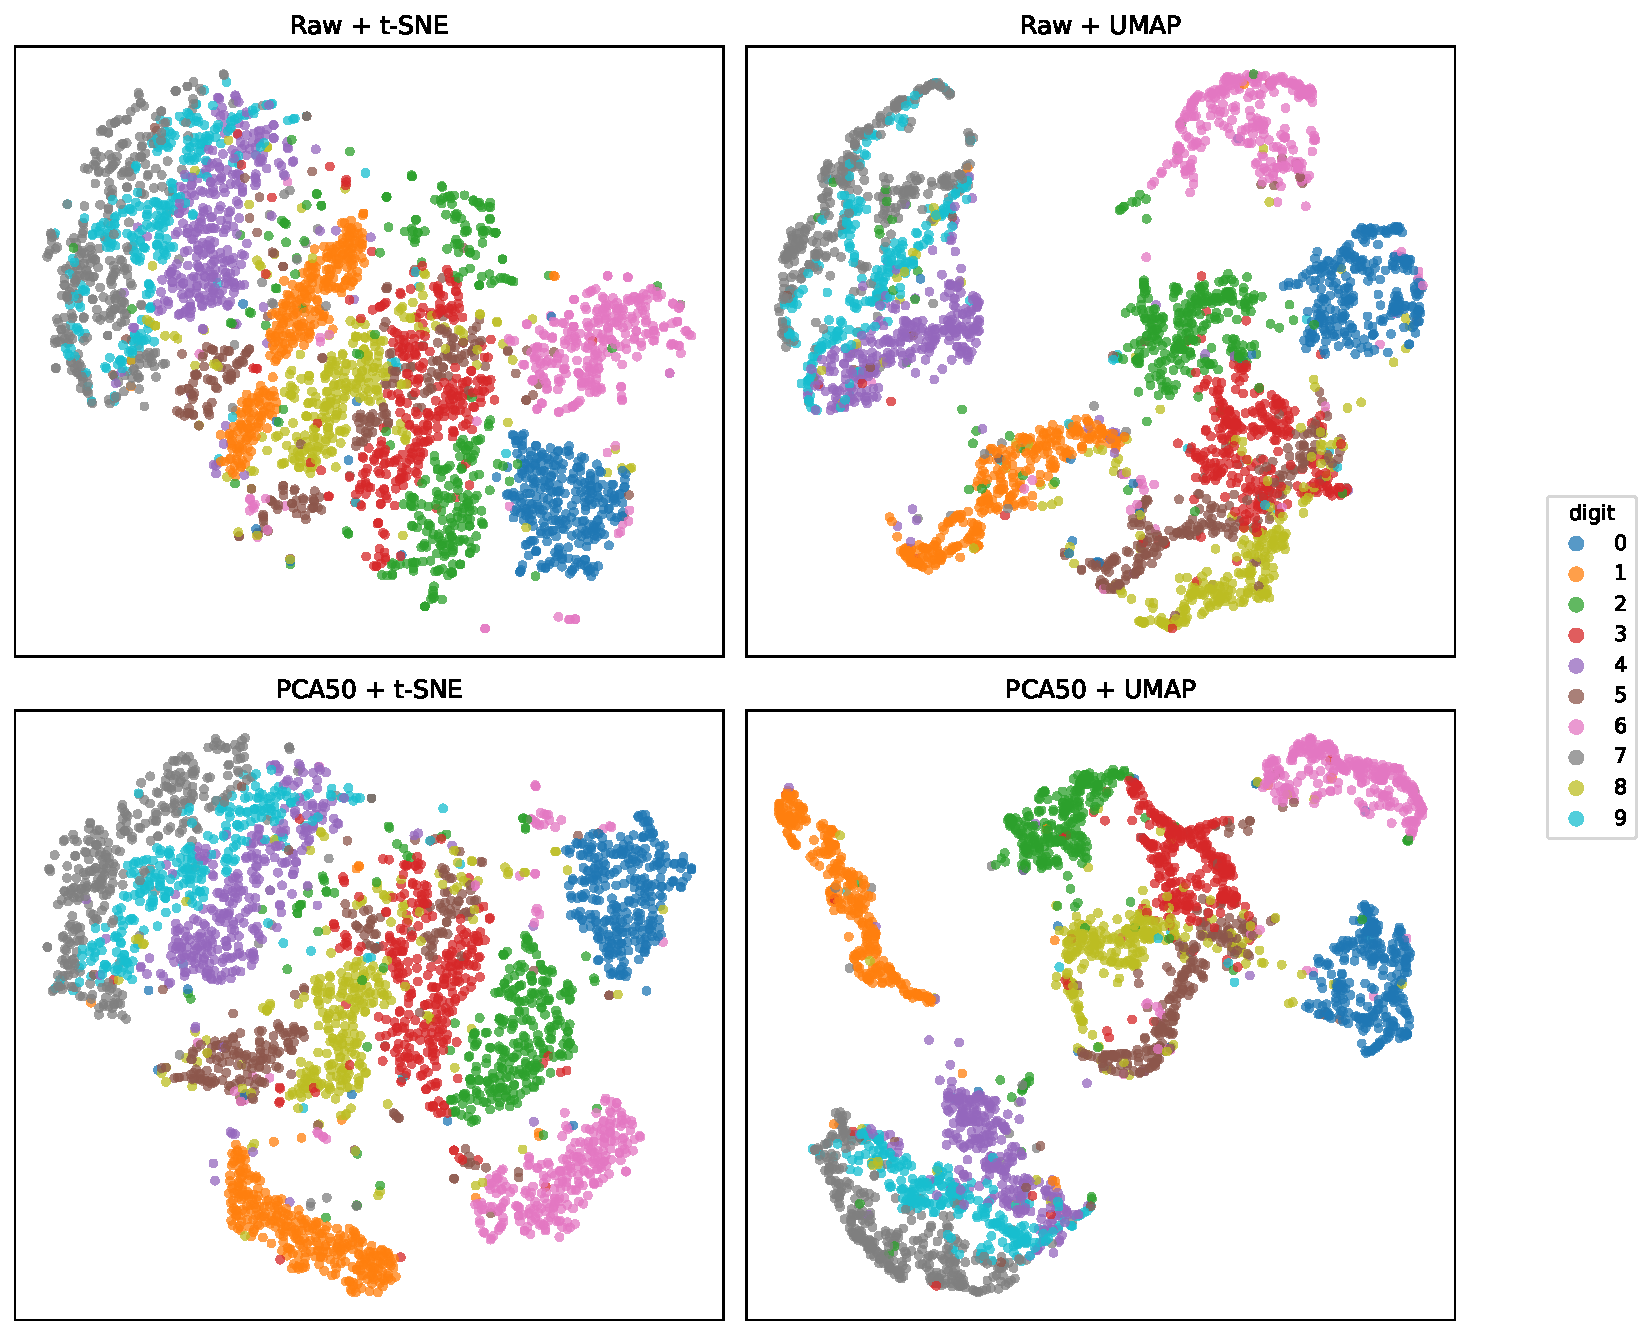
\includegraphics[keepaspectratio]{contents/3/embedding_files/figure-pdf/cell-14-output-1.pdf}}

Since neither method aims to preserve global geometry, we focus on the
stability of local neighborhoods and on the qualitative differences
between the resulting embeddings.

The figure highlights two main comparisons: the effect of PCA
preprocessing and the differences between t-SNE and UMAP.

\begin{center}\rule{0.5\linewidth}{0.5pt}\end{center}

Raw versus PCA50

\begin{itemize}
\tightlist
\item
  In this MNIST subset, applying PCA before t-SNE or UMAP changes the
  exact layout but preserves much of the local neighborhood structure.
  The PCA50 embeddings therefore produce similar digit neighborhoods
  while reducing the dimensionality from 784 to 50.
\item
  In this example, the PCA50 embeddings appear slightly cleaner, with
  fewer scattered points and more coherent local neighborhoods. In
  practice, PCA preprocessing can improve computational efficiency and
  reduce low-variance noise while retaining much of the information
  needed for nonlinear visualization.
\end{itemize}

\begin{center}\rule{0.5\linewidth}{0.5pt}\end{center}

t-SNE versus UMAP

\begin{itemize}
\tightlist
\item
  Both methods recover clear local neighborhoods for the handwritten
  digits. Images with the same label tend to occupy nearby regions,
  although several visually similar digit classes still overlap.
\item
  With these settings, the UMAP embeddings show several groups of
  similar digits as relatively well-separated neighboring regions. For
  example, groups of visually similar digits, such as 3, 5, and 8 or 4,
  7, and 9, tend to occupy neighboring regions, reflecting similarities
  in their handwritten shapes.
\item
  With these settings, the t-SNE embeddings connect these similar digit
  classes through more gradual transitions. Instead of forming clearly
  separated islands, neighboring classes blend through intermediate
  handwriting styles, giving the overall layout a more continuous
  appearance.
\end{itemize}

These differences should be read as differences in the visualization
objectives, not as proof that one method has found the true geometry.
UMAP's clearer separation and t-SNE's smoother transitions are both
diagnostic patterns to investigate, not final cluster definitions.

\subsection{Four-method comparison}\label{four-method-comparison}

PCA, spectral embedding, t-SNE, and UMAP all create low-dimensional
coordinates, but they answer different diagnostic questions. PCA is the
linear baseline. Spectral embedding is graph-based and focuses on
connectivity. t-SNE focuses on local neighbor probabilities. UMAP
focuses on a weighted nearest-neighbor graph.

{\def\LTcaptype{none} % do not increment counter
\begin{longtable}[]{@{}
  >{\raggedright\arraybackslash}p{(\linewidth - 6\tabcolsep) * \real{0.2500}}
  >{\raggedright\arraybackslash}p{(\linewidth - 6\tabcolsep) * \real{0.2500}}
  >{\raggedright\arraybackslash}p{(\linewidth - 6\tabcolsep) * \real{0.2500}}
  >{\raggedright\arraybackslash}p{(\linewidth - 6\tabcolsep) * \real{0.2500}}@{}}
\toprule\noalign{}
\begin{minipage}[b]{\linewidth}\raggedright
Method
\end{minipage} & \begin{minipage}[b]{\linewidth}\raggedright
Mainly preserves
\end{minipage} & \begin{minipage}[b]{\linewidth}\raggedright
Does not preserve well
\end{minipage} & \begin{minipage}[b]{\linewidth}\raggedright
Best for checking
\end{minipage} \\
\midrule\noalign{}
\endhead
\bottomrule\noalign{}
\endlastfoot
PCA & linear variance and large-scale linear directions & nonlinear
neighborhoods and curved manifolds & whether a simple linear projection
already explains the main variation \\
Spectral embedding & connectivity in a chosen graph & original feature
axes and exact Euclidean distances & whether a nearest-neighbor graph
separates groups \\
PCA50 + t-SNE & local neighborhood probabilities after PCA preprocessing
& global distances, island sizes, densities, axis directions & whether
local neighborhoods or clustering labels are visually mixed \\
PCA50 + UMAP & local nearest-neighbor graph after PCA preprocessing,
with some broader structure depending on \texttt{n\_neighbors} & exact
distances, densities, and axis meanings & nonlinear local visualization
and graph-based neighborhood structure \\
\end{longtable}
}

We now apply all four methods to the same MNIST subset. PCA and spectral
embedding are applied to the standardized pixel features, while t-SNE
and UMAP are applied after PCA preprocessing to 50 dimensions.

\begin{Shaded}
\begin{Highlighting}[]
\ImportTok{from}\NormalTok{ sklearn.manifold }\ImportTok{import}\NormalTok{ SpectralEmbedding}
\NormalTok{Z\_pca2 }\OperatorTok{=}\NormalTok{ PCA(n\_components}\OperatorTok{=}\DecValTok{2}\NormalTok{, random\_state}\OperatorTok{=}\DecValTok{1}\NormalTok{).fit\_transform(X\_mnist)}

\NormalTok{Z\_spectral\_mnist }\OperatorTok{=}\NormalTok{ SpectralEmbedding(}
\NormalTok{    n\_components}\OperatorTok{=}\DecValTok{2}\NormalTok{,}
\NormalTok{    affinity}\OperatorTok{=}\StringTok{"nearest\_neighbors"}\NormalTok{,}
\NormalTok{    n\_neighbors}\OperatorTok{=}\DecValTok{15}\NormalTok{,}
\NormalTok{    random\_state}\OperatorTok{=}\DecValTok{1}\NormalTok{,}
\NormalTok{).fit\_transform(X\_mnist)}

\NormalTok{embeddings }\OperatorTok{=}\NormalTok{ \{}
    \StringTok{"PCA"}\NormalTok{: (Z\_pca2, }\StringTok{"PC1"}\NormalTok{, }\StringTok{"PC2"}\NormalTok{),}
    \StringTok{"Spectral embedding"}\NormalTok{: (Z\_spectral\_mnist, }\StringTok{"SE1"}\NormalTok{, }\StringTok{"SE2"}\NormalTok{),}
    \StringTok{"PCA50 + t{-}SNE"}\NormalTok{: (Z\_tsne\_compare, }\StringTok{"t{-}SNE1"}\NormalTok{, }\StringTok{"t{-}SNE2"}\NormalTok{),}
    \StringTok{"PCA50 + UMAP"}\NormalTok{: (Z\_umap\_compare, }\StringTok{"UMAP1"}\NormalTok{, }\StringTok{"UMAP2"}\NormalTok{),}
\NormalTok{\}}

\NormalTok{fig, axs }\OperatorTok{=}\NormalTok{ plt.subplots(}\DecValTok{2}\NormalTok{, }\DecValTok{2}\NormalTok{, figsize}\OperatorTok{=}\NormalTok{(}\DecValTok{11}\NormalTok{, }\DecValTok{9}\NormalTok{))}

\NormalTok{scatter }\OperatorTok{=} \VariableTok{None}
\ControlFlowTok{for}\NormalTok{ ax, (name, (Z\_method, xlabel, ylabel)) }\KeywordTok{in} \BuiltInTok{zip}\NormalTok{(axs.ravel(), embeddings.items()):}
\NormalTok{    scatter }\OperatorTok{=}\NormalTok{ ax.scatter(}
\NormalTok{        Z\_method[:, }\DecValTok{0}\NormalTok{],}
\NormalTok{        Z\_method[:, }\DecValTok{1}\NormalTok{],}
\NormalTok{        c}\OperatorTok{=}\NormalTok{y\_mnist,}
\NormalTok{        cmap}\OperatorTok{=}\StringTok{"tab10"}\NormalTok{,}
\NormalTok{        s}\OperatorTok{=}\DecValTok{10}\NormalTok{,}
\NormalTok{        alpha}\OperatorTok{=}\FloatTok{0.75}\NormalTok{,}
\NormalTok{    )}
\NormalTok{    ax.set\_title(name)}
\NormalTok{    ax.set\_xlabel(xlabel)}
\NormalTok{    ax.set\_ylabel(ylabel)}
\NormalTok{    ax.set\_xticks([])}
\NormalTok{    ax.set\_yticks([])}

\NormalTok{fig.legend(}\OperatorTok{*}\NormalTok{scatter.legend\_elements(), title}\OperatorTok{=}\StringTok{"digit"}\NormalTok{, loc}\OperatorTok{=}\StringTok{"center right"}\NormalTok{)}
\NormalTok{fig.tight\_layout(rect}\OperatorTok{=}\NormalTok{[}\DecValTok{0}\NormalTok{, }\DecValTok{0}\NormalTok{, }\FloatTok{0.9}\NormalTok{, }\DecValTok{1}\NormalTok{])}\OperatorTok{;}
\end{Highlighting}
\end{Shaded}

\pandocbounded{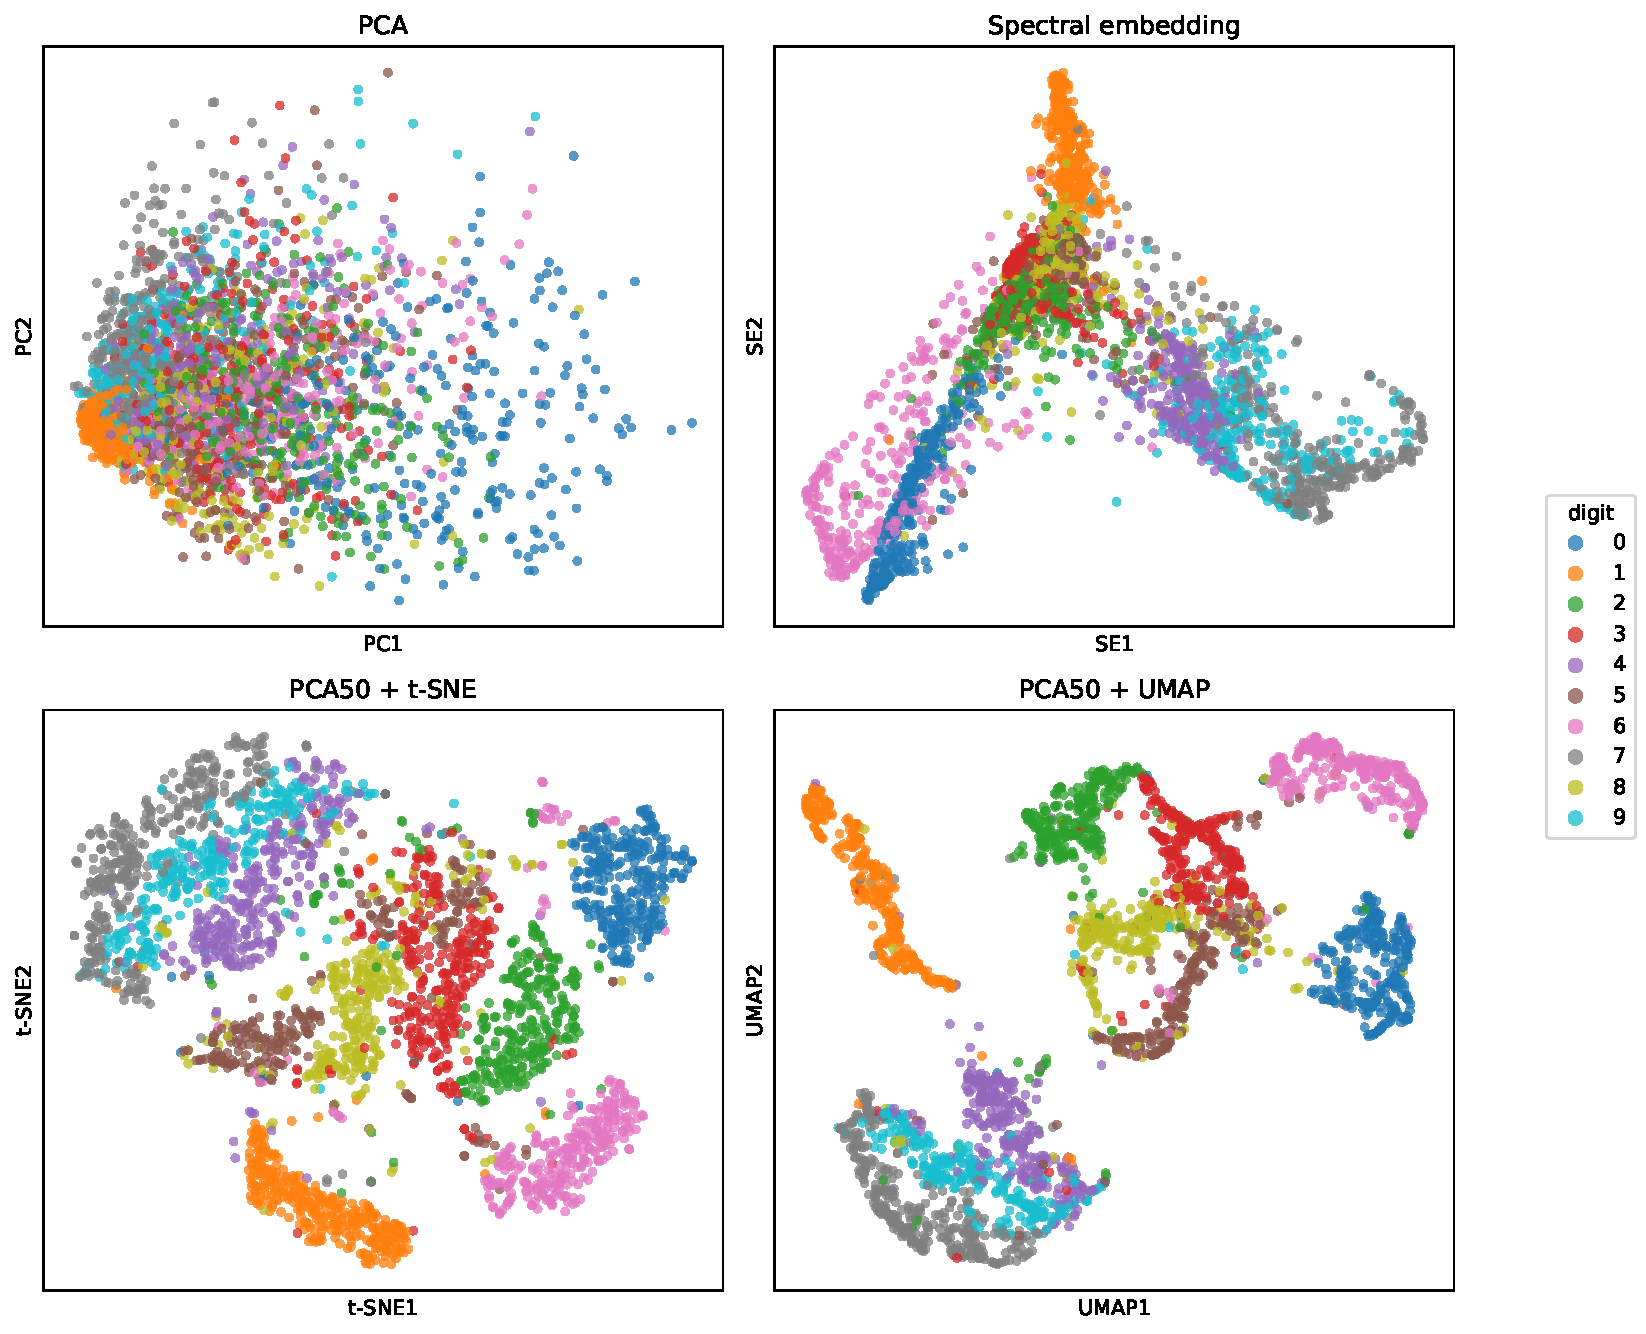
\includegraphics[keepaspectratio]{contents/3/embedding_files/figure-pdf/cell-15-output-1.pdf}}

The four methods provide different views of the same high-dimensional
image subset because they preserve different aspects of the original
data. Some observations from the comparison are:

\begin{itemize}
\tightlist
\item
  PCA provides the linear reference view by projecting the images onto
  two directions of maximum variance. It captures the dominant linear
  variation but leaves substantial overlap because the digit classes are
  not linearly separable.
\item
  Spectral embedding reveals nonlinear organization that is not visible
  in the PCA projection. Because the embedding is constructed from a
  nearest-neighbor graph, the resulting layout depends strongly on the
  chosen graph.
\item
  PCA50 + t-SNE and PCA50 + UMAP recover many of the same local
  neighborhoods, but organize them differently because they optimize
  different objective functions.
\end{itemize}

The four methods should therefore be interpreted differently because
each is designed to preserve a different aspect of the original data.
PCA asks whether a low-dimensional linear projection already captures
the dominant variation. Spectral embedding asks whether a neighborhood
graph reveals meaningful connected structure. t-SNE asks whether local
neighborhoods remain coherent after embedding. UMAP asks whether the
nearest-neighbor graph exhibits stable graph-connected regions. None of
these methods provides a geometrically faithful map of the original
feature space. Their interpretation should therefore always be based on
the structure each method is designed to preserve.

\begin{tcolorbox}[enhanced jigsaw, arc=.35mm, bottomrule=.15mm, bottomtitle=1mm, breakable, colback=white, colbacktitle=quarto-callout-note-color!10!white, colframe=quarto-callout-note-color-frame, coltitle=black, left=2mm, leftrule=.75mm, opacityback=0, opacitybacktitle=0.6, rightrule=.15mm, title=\textcolor{quarto-callout-note-color}{\faInfo}\hspace{0.5em}{Using all 70,000 MNIST images}, titlerule=0mm, toprule=.15mm, toptitle=1mm]

The examples above use a fixed subset of 3,000 images for speed. The
next two figures repeat the previous comparisons using the full MNIST
dataset with 70,000 images. The first figure compares t-SNE and UMAP,
with or without PCA, and the second figure compares PCA, spectral
embedding, PCA50 + t-SNE, and PCA50 + UMAP.

\begin{figure}[H]

\centering{

\pandocbounded{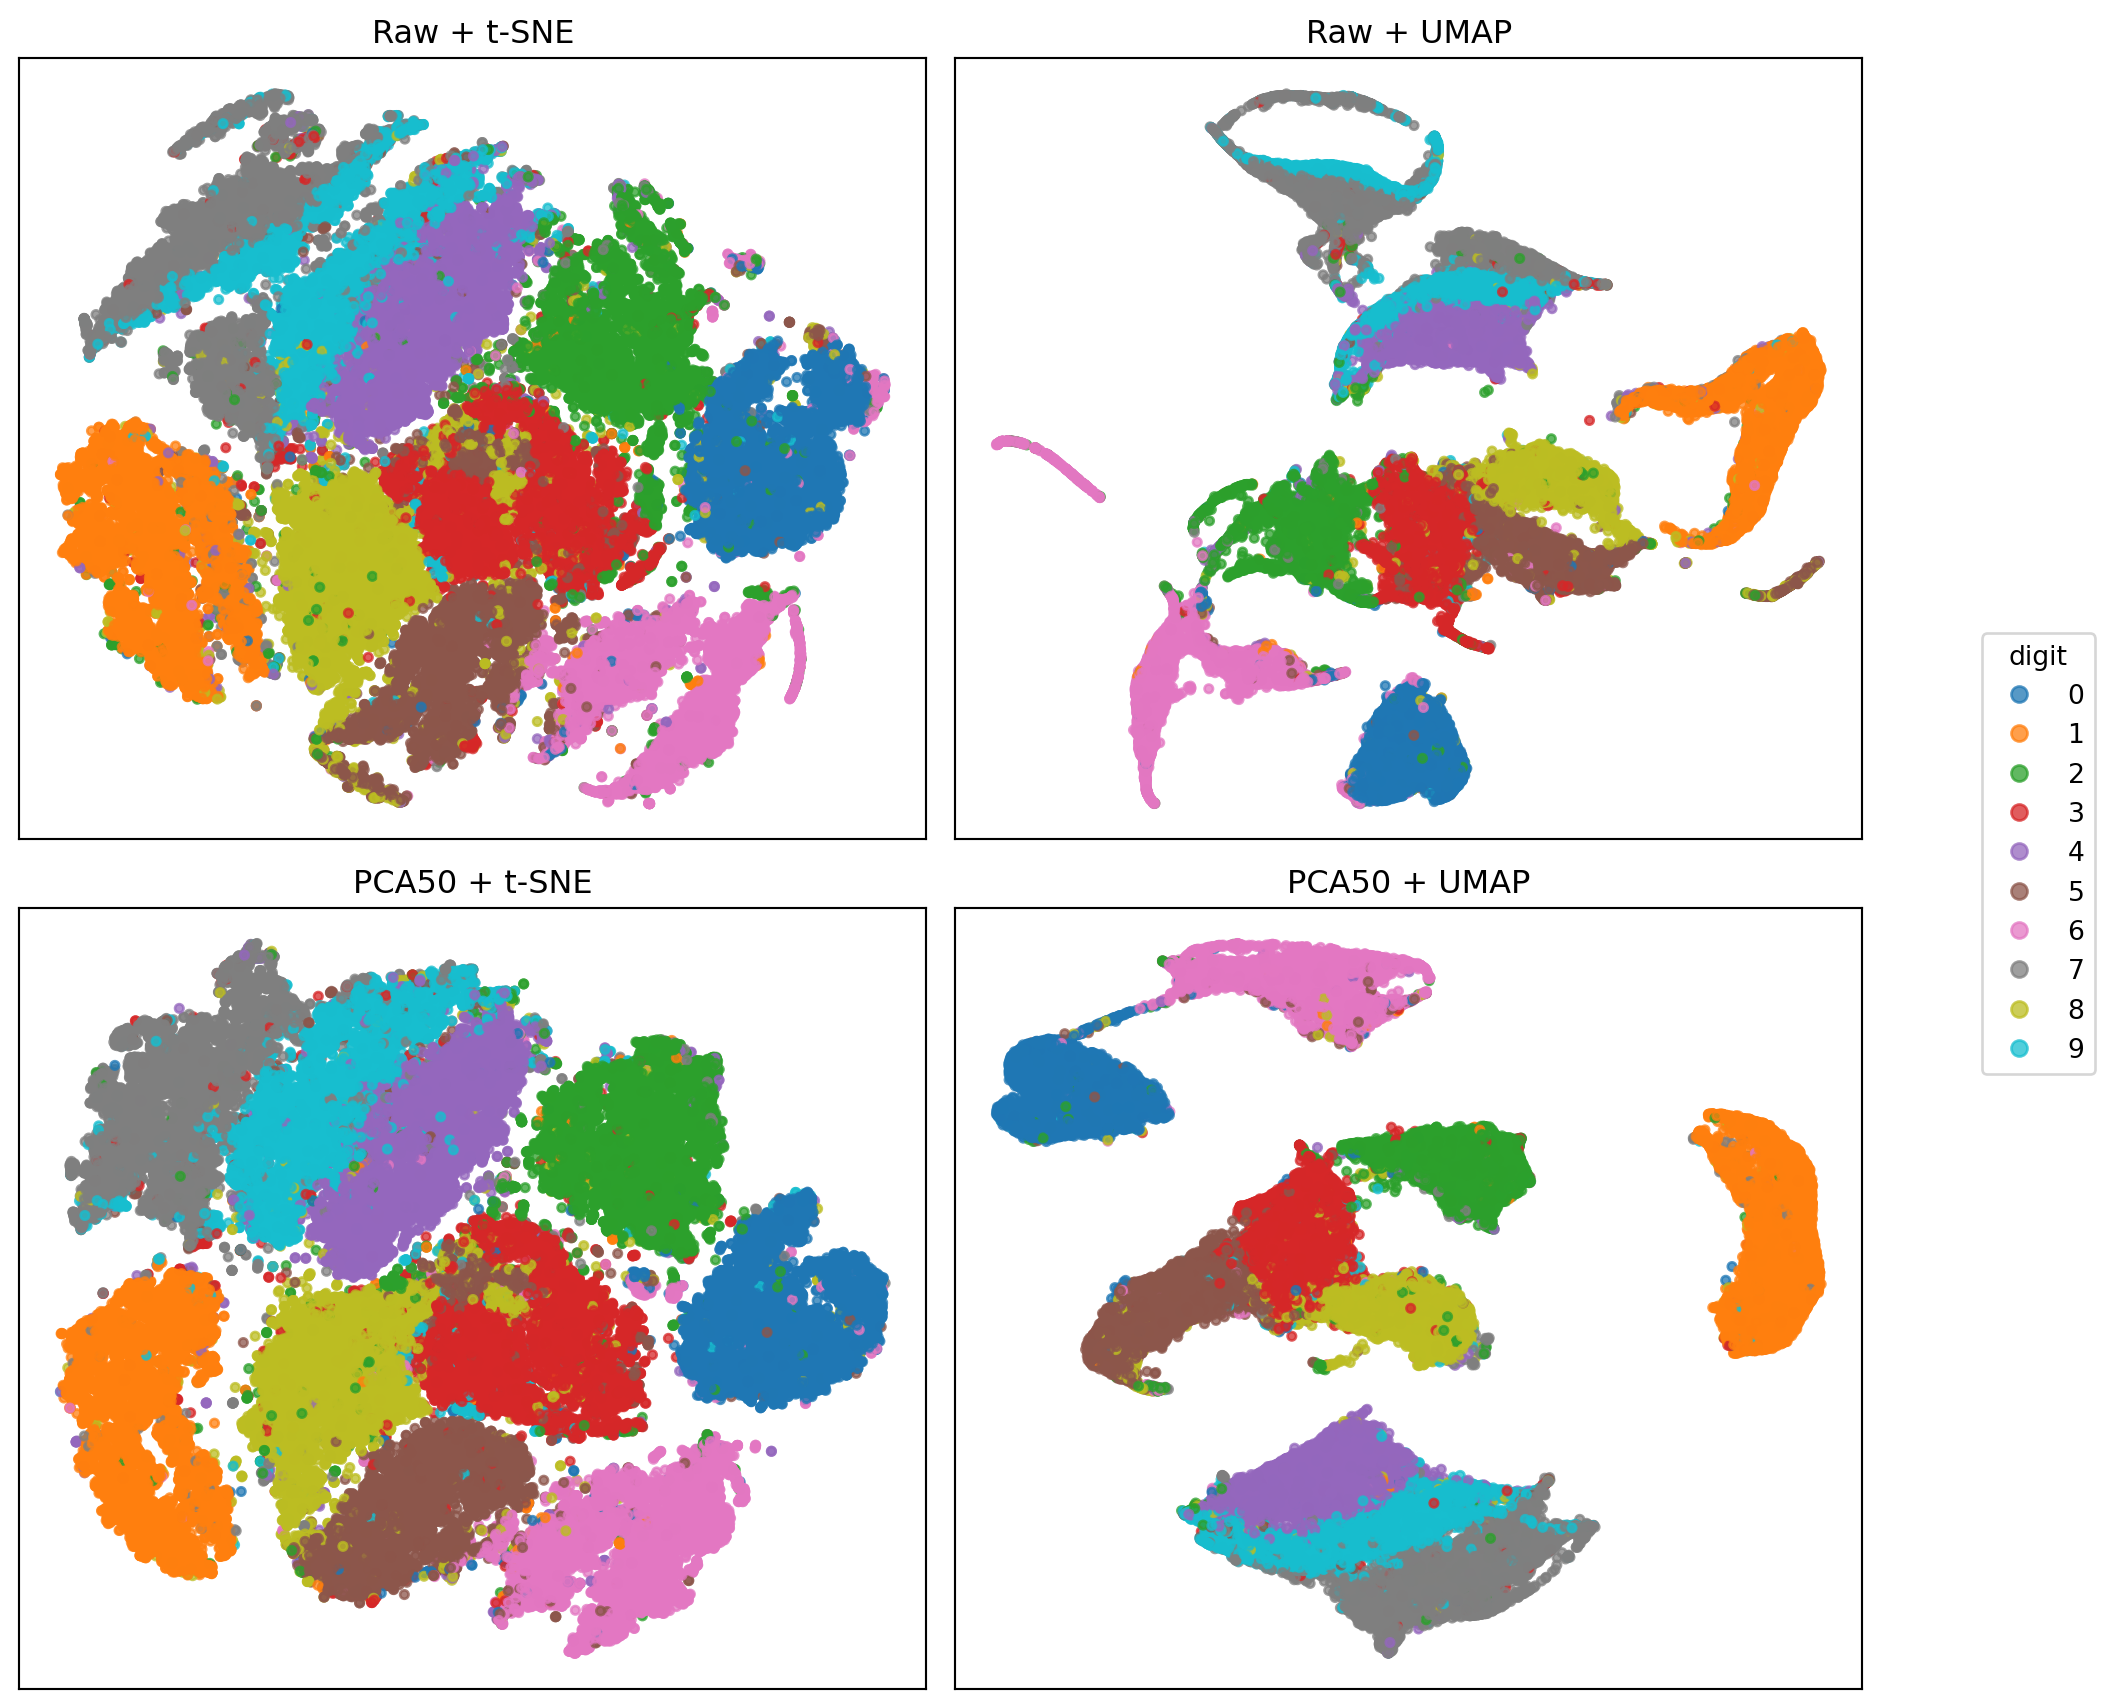
\includegraphics[keepaspectratio]{contents/3/images/70k-1.png}}

}

\caption{\label{fig-mnist-70k-tsne-umap}t-SNE and UMAP comparison on all
70,000 MNIST images}

\end{figure}%

\begin{figure}[H]

\centering{

\pandocbounded{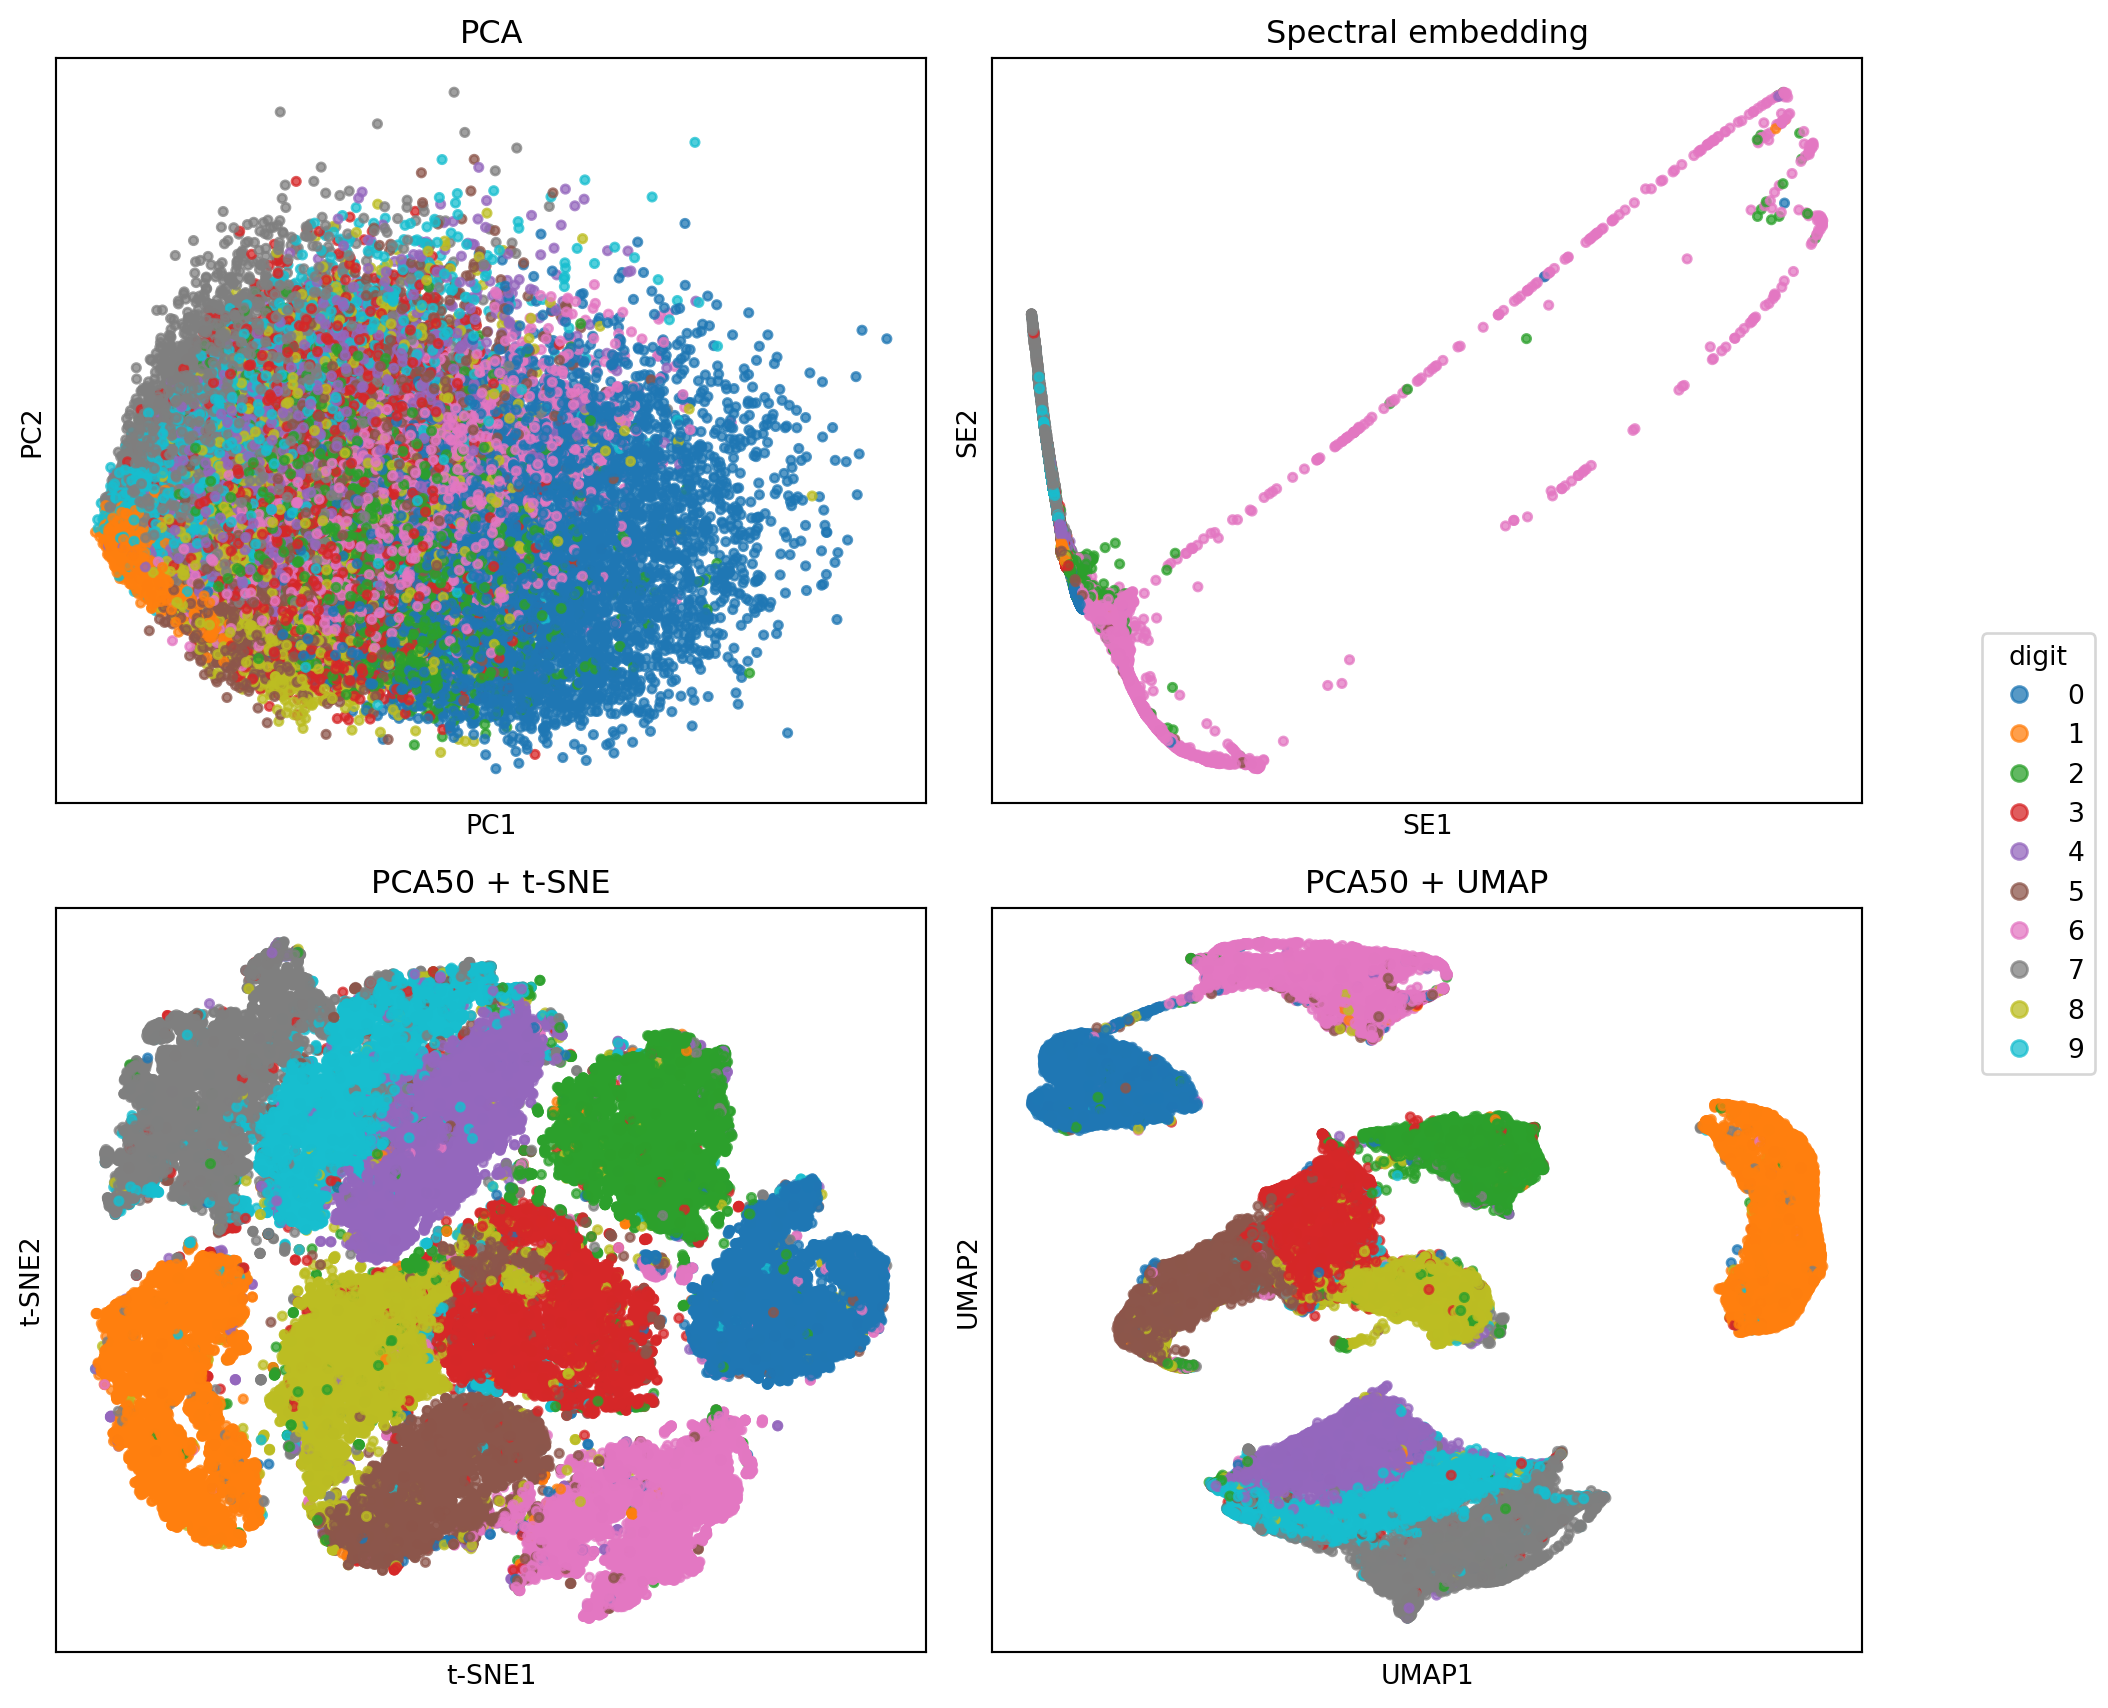
\includegraphics[keepaspectratio]{contents/3/images/70k-2.png}}

}

\caption{\label{fig-mnist-70k-four-methods}Four-method comparison on all
70,000 MNIST images}

\end{figure}%

Compared with the 3,000-image subset:

\begin{itemize}
\tightlist
\item
  The main qualitative conclusions are broadly similar. The 3,000-image
  subset already captures many of the important neighborhood
  relationships among the handwritten digits.
\item
  The plots become visually denser with 70,000 images because many more
  intermediate handwriting styles are included.
\item
  PCA changes the least: the dominant linear directions remain similar,
  and the larger dataset mainly increases sampling density.
\item
  Spectral embedding becomes smoother because the nearest-neighbor graph
  is constructed from many more observations, making graph branches more
  complete and less affected by sampling variability.
\item
  The t-SNE embedding becomes substantially denser. Many apparent gaps
  between neighboring digit groups are filled by intermediate
  observations, producing smoother local transitions.
\item
  The UMAP embedding also becomes denser while retaining more clearly
  segmented graph-connected regions.
\item
  Increasing the sample size improves the completeness and stability of
  the visualizations, but it does not make global distances, region
  sizes, or visual densities quantitatively reliable.
\item
  Running t-SNE and UMAP on all 70,000 images is substantially more
  computationally expensive than using a representative 3,000-image
  subset.
\end{itemize}

\end{tcolorbox}

\begin{tcolorbox}[enhanced jigsaw, arc=.35mm, bottomrule=.15mm, bottomtitle=1mm, breakable, colback=white, colbacktitle=quarto-callout-caution-color!10!white, colframe=quarto-callout-caution-color-frame, coltitle=black, left=2mm, leftrule=.75mm, opacityback=0, opacitybacktitle=0.6, rightrule=.15mm, title=\textcolor{quarto-callout-caution-color}{\faFire}\hspace{0.5em}{Apparent clusters are not proof of clusters}, titlerule=0mm, toprule=.15mm, toptitle=1mm]

Visible separation in an embedding is a diagnostic clue, not a cluster
definition by itself. A gap, island, or bridge should be checked against
the structure the method is designed to preserve and, when needed,
against quantitative criteria tied to the analysis goal.

\end{tcolorbox}

\cleardoublepage
\phantomsection
\addcontentsline{toc}{part}{Appendices}
\appendix

\chapter{Python IDE Setup}\label{python-ide-setup}

There are many ways to set up a Python development environment, and each
has its own advantages and disadvantages. In this tutorial, we will
cover one of the most popular current setups: VS Code + \texttt{uv}.

For now, we will focus only on the practical setup steps. The underlying
concepts will be discussed in the later appendices.

This tutorial uses Windows 11. If you use another operating system, the
steps are very similar, but you may need to make some minor but
straightforward modifications. If you encounter major issues, please
contact me.

\section{VS Code}\label{sec-vscode}

We choose VS Code as our IDE for Python. The installation is
straightforward starting from the
\href{https://code.visualstudio.com/}{Official website}. After
installation, we need to do a few configurations to make the experience
better.

\begin{enumerate}
\def\labelenumi{\arabic{enumi}.}
\tightlist
\item
  For development of Python, the essential plugins are the Python plugin
  and Jupyter plugin. You only need to install the two main ones, and
  all related plugins will be installed automatically.
\end{enumerate}

\pandocbounded{
\includegraphics[keepaspectratio]{contents/app/assets/img/20250811114515.png}}

You may either search the extensions directly from VS Code extension tab
(which is usually located on the left side bar), or you may install it
from the link
\href{https://marketplace.visualstudio.com/items?itemName=ms-python.python}{python}
and
\href{https://marketplace.visualstudio.com/items?itemName=ms-toolsai.jupyter}{jupyter}.

\begin{enumerate}
\def\labelenumi{\arabic{enumi}.}
\setcounter{enumi}{1}
\tightlist
\item
  Sometimes you may need to use the terminal inside VS Code. You may
  start the terminal from top menu (whose hotkey is by default
  \texttt{ctrl+shift+\textasciigrave{}}).
\end{enumerate}

\pandocbounded{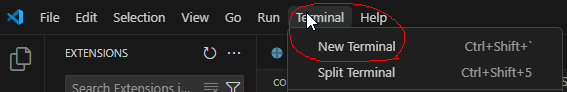
\includegraphics[keepaspectratio]{contents/app/assets/img/20250811113649.png}}

Note that there are many different choices of terminals. After you start
the first default terminal, you may start any new terminals using the
small \texttt{+} and the \texttt{v} mark on the right.

\pandocbounded{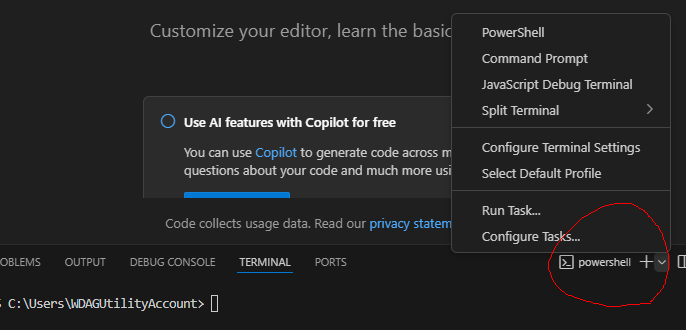
\includegraphics[keepaspectratio]{contents/app/assets/img/20250811120220.png}}

\begin{tcolorbox}[enhanced jigsaw, arc=.35mm, bottomrule=.15mm, bottomtitle=1mm, breakable, colback=white, colbacktitle=quarto-callout-caution-color!10!white, colframe=quarto-callout-caution-color-frame, coltitle=black, left=2mm, leftrule=.75mm, opacityback=0, opacitybacktitle=0.6, rightrule=.15mm, title=\textcolor{quarto-callout-caution-color}{\faFire}\hspace{0.5em}{Change Terminal default profile}, titlerule=0mm, toprule=.15mm, toptitle=1mm]

In Windows the default terminal is Powershell when you first install VS
Code. In the past it had bugs with \texttt{conda} (and I don't know
whether it is fixed now). In order to avoid headaches due to the bugs,
we simply switch to other terminals, like Command Prompt. You may change
the default terminal by

\begin{enumerate}
\def\labelenumi{\arabic{enumi}.}
\tightlist
\item
  Press \texttt{Ctrl+Shift+P} or \texttt{F1} to open the top prompt
  menu.
\item
  Find the \texttt{Terminal:\ Select\ Default\ Profile} command.
\end{enumerate}

\pandocbounded{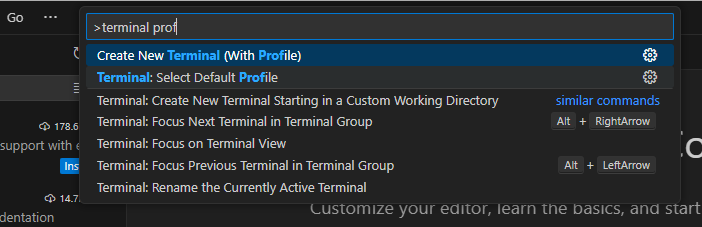
\includegraphics[keepaspectratio]{contents/app/assets/img/20250811114818.png}}

\begin{enumerate}
\def\labelenumi{\arabic{enumi}.}
\setcounter{enumi}{2}
\tightlist
\item
  Select the desired terminal as the default one.
\end{enumerate}

\pandocbounded{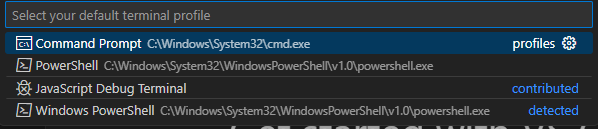
\includegraphics[keepaspectratio]{contents/app/assets/img/20250811114921.png}}

\end{tcolorbox}

\section{Python Virtual Environment
installation}\label{python-virtual-environment-installation}

There are many tools available for managing Python environments and
packages. As of Summer 2026, \texttt{uv} has become one of the most
popular choices.

\texttt{uv} is an all-in-one tool for managing Python installations,
virtual environments, and project dependencies. With \texttt{uv}, you do
not need to install Python separately, as it can download and manage
Python versions for you. You may visit the
\href{https://docs.astral.sh/uv/getting-started/installation/}{official
documentation} to install \texttt{uv}.

\begin{tcolorbox}[enhanced jigsaw, arc=.35mm, bottomrule=.15mm, bottomtitle=1mm, breakable, colback=white, colbacktitle=quarto-callout-caution-color!10!white, colframe=quarto-callout-caution-color-frame, coltitle=black, left=2mm, leftrule=.75mm, opacityback=0, opacitybacktitle=0.6, rightrule=.15mm, title=\textcolor{quarto-callout-caution-color}{\faFire}\hspace{0.5em}{Windows headache}, titlerule=0mm, toprule=.15mm, toptitle=1mm]

There is a possibility that Smart App Control (SAC) or other Application
Control policies in Windows 11 may block the execution of
\texttt{uv.exe}. In this case, you may see a message similar to

\begin{Shaded}
\begin{Highlighting}[]
\NormalTok{\textquotesingle{}C:\textbackslash{}Users\textbackslash{}WDAGUtilityAccount\textbackslash{}.local\textbackslash{}bin\textbackslash{}uv.exe\textquotesingle{}}
\NormalTok{was blocked by your organization\textquotesingle{}s Device Guard policy.}
\NormalTok{Contact your support person for more info.}
\end{Highlighting}
\end{Shaded}

This may occur because Windows does not yet consider the executable
sufficiently trusted under its application-control policies.

If this happens, note that the exact cause and solution can vary across
machines, Windows versions, and security configurations. In addition,
both Windows and \texttt{uv} are evolving rapidly, so solutions that
work today may change in the future.

You are encouraged to search for the solution that best fits your
situation. For this course, one workaround is to use WSL (see
Section~\ref{sec-wsl}).

\end{tcolorbox}

After installation (and you may need to restart VS Code or open a new
terminal window so that the \texttt{uv} command becomes available), you
can use the following commands to verify that \texttt{uv} is working
correctly.

{\def\LTcaptype{none} % do not increment counter
\begin{longtable}[]{@{}
  >{\raggedright\arraybackslash}p{(\linewidth - 4\tabcolsep) * \real{0.3333}}
  >{\raggedright\arraybackslash}p{(\linewidth - 4\tabcolsep) * \real{0.3333}}
  >{\raggedright\arraybackslash}p{(\linewidth - 4\tabcolsep) * \real{0.3333}}@{}}
\toprule\noalign{}
\begin{minipage}[b]{\linewidth}\raggedright
Command
\end{minipage} & \begin{minipage}[b]{\linewidth}\raggedright
Purpose
\end{minipage} & \begin{minipage}[b]{\linewidth}\raggedright
Example Output
\end{minipage} \\
\midrule\noalign{}
\endhead
\bottomrule\noalign{}
\endlastfoot
\texttt{uv\ -\/-version} & Display the installed \texttt{uv} version.
Useful for verifying that \texttt{uv} is installed correctly. &
\texttt{uv\ 0.11.17} \\
\texttt{uv\ self\ update} & Update \texttt{uv} itself to the latest
available version. Similar to updating package managers such as
\texttt{pip} or \texttt{cargo}. &
\texttt{Upgraded\ uv\ from\ v0.11.4\ to\ v0.11.17!} \\
\texttt{uv\ python\ list} & Show all Python versions available locally
and those that can be installed through \texttt{uv}. & Lists installed
and downloadable Python versions. \\
\end{longtable}
}

\subsection{Install the first Python}\label{install-the-first-python}

Since VS Code often expects to discover at least one Python interpreter
before it can fully initialize its Python and Jupyter services, we first
install a Python version managed by \texttt{uv}.

\begin{Shaded}
\begin{Highlighting}[]
\ExtensionTok{uv}\NormalTok{ python install}
\end{Highlighting}
\end{Shaded}

This Python installation is managed entirely by \texttt{uv}; it is not
intended to be used directly for course work. Instead, it serves as a
bootstrap interpreter that allows VS Code to detect Python correctly and
manage project-specific virtual environments more reliably. You can
verify the installed Python versions using \texttt{uv\ python\ list} as
mentioned above.

If you skip this step and directly jump into the virtual environment,
there is a possibility that Python in VS Code doesn't work well.

\subsection{Setup the environment for the
course}\label{setup-the-environment-for-the-course}

To set up the environment for this course, we provide the
\href{../../pyproject.toml}{toml file} and
\href{../../.python-version}{python version file} for this course.

Alternatively, you may create a file named \texttt{pyproject.toml} and
add the following content:

\begin{Shaded}
\begin{Highlighting}[]
\KeywordTok{[project]}
\DataTypeTok{name} \OperatorTok{=} \StringTok{"STAT432"}
\DataTypeTok{version} \OperatorTok{=} \StringTok{"0.1.0"}
\DataTypeTok{requires{-}python} \OperatorTok{=} \StringTok{"\textgreater{}=3.13"}
\DataTypeTok{dependencies} \OperatorTok{=} \OperatorTok{[}
    \StringTok{"jupyter\textgreater{}=1.1.1"}\OperatorTok{,}
    \StringTok{"matplotlib\textgreater{}=3.10.9"}\OperatorTok{,}
    \StringTok{"pandas\textgreater{}=3.0.2"}\OperatorTok{,}
    \StringTok{"scikit{-}learn\textgreater{}=1.8.0"}\OperatorTok{,}
    \StringTok{"seaborn\textgreater{}=0.13.2"}\OperatorTok{,}
    \StringTok{"statsmodels\textgreater{}=0.14.6"}\OperatorTok{,}
    \StringTok{"xgboost\textgreater{}=3.2.0"}\OperatorTok{,}
\OperatorTok{]}
\end{Highlighting}
\end{Shaded}

The python version file only contains the version number \texttt{3.13}
inside since this is the version of Python I use when I wrote the notes.
You may either download the file and put it inside the folder or create
a file with the name \texttt{.python-version} and write \texttt{3.13}
inside.

\begin{tcolorbox}[enhanced jigsaw, arc=.35mm, bottomrule=.15mm, bottomtitle=1mm, breakable, colback=white, colbacktitle=quarto-callout-warning-color!10!white, colframe=quarto-callout-warning-color-frame, coltitle=black, left=2mm, leftrule=.75mm, opacityback=0, opacitybacktitle=0.6, rightrule=.15mm, title=\textcolor{quarto-callout-warning-color}{\faExclamationTriangle}\hspace{0.5em}{Autosave}, titlerule=0mm, toprule=.15mm, toptitle=1mm]

Before proceeding, make sure the file is saved.

By default, VS Code does not enable Auto Save. If you see a small dot
next to the file name, the file contains unsaved changes.

\pandocbounded{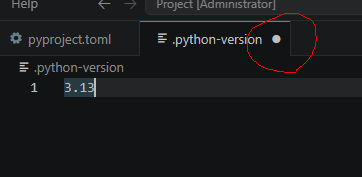
\includegraphics[keepaspectratio]{contents/app/assets/img/20260529122024.png}}

Many beginner problems occur because they modify a file but forget to
save it before running commands.

\end{tcolorbox}

\begin{enumerate}
\def\labelenumi{\arabic{enumi}.}
\tightlist
\item
  Create a new folder. The folder name is irrelevant. Put the files
  \texttt{pyproject.toml} and \texttt{.python-version} in the folder.
\item
  Open a terminal (no matter whether within VS Code or not) and enter
  the folder. Use the command \texttt{uv\ sync}.
\end{enumerate}

After the command finishes, \texttt{uv} creates a virtual environment
named \texttt{.venv} and installs all required packages specified in
\texttt{pyproject.toml}. The resulting environment should closely match
the one used to prepare these notes.

Now it is possible to start using the virtual environment for the
course. In case that you need to modify the virtual environment, please
continue the read the following optional part.

\begin{tcolorbox}[enhanced jigsaw, arc=.35mm, bottomrule=.15mm, bottomtitle=1mm, breakable, colback=white, colbacktitle=quarto-callout-note-color!10!white, colframe=quarto-callout-note-color-frame, coltitle=black, left=2mm, leftrule=.75mm, opacityback=0, opacitybacktitle=0.6, rightrule=.15mm, title=\textcolor{quarto-callout-note-color}{\faInfo}\hspace{0.5em}{Modifying the Environment}, titlerule=0mm, toprule=.15mm, toptitle=1mm]

To install a package and update the project configuration, use
\texttt{uv\ add\ \textless{}package-name\textgreater{}}.

For example, you may need \texttt{openpyxl} to read and write Excel
files:

\begin{Shaded}
\begin{Highlighting}[]
\ExtensionTok{uv}\NormalTok{ add openpyxl}
\end{Highlighting}
\end{Shaded}

This command updates the project configuration in
\texttt{pyproject.toml} and installs the package into the project's
virtual environment \texttt{.venv}.

Most package management tasks can be handled through \texttt{uv\ add}.

\end{tcolorbox}

\begin{tcolorbox}[enhanced jigsaw, arc=.35mm, bottomrule=.15mm, bottomtitle=1mm, breakable, colback=white, colbacktitle=quarto-callout-note-color!10!white, colframe=quarto-callout-note-color-frame, coltitle=black, left=2mm, leftrule=.75mm, opacityback=0, opacitybacktitle=0.6, rightrule=.15mm, title=\textcolor{quarto-callout-note-color}{\faInfo}\hspace{0.5em}{Jupyter kernels and modifying venv}, titlerule=0mm, toprule=.15mm, toptitle=1mm]

A Jupyter kernel is the Python environment used by a notebook. When a
notebook cell is executed, the code runs inside the selected kernel.
Therefore, it is important to connect the notebook to the kernel
associated with your course environment.

Modern versions of VS Code can usually detect a project managed by
\texttt{uv} and use it directly as a notebook kernel. In many cases, no
manual kernel registration is required. If VS Code does not
automatically detect the environment, you can create a dedicated Jupyter
kernel:

\begin{Shaded}
\begin{Highlighting}[]
\ExtensionTok{uv}\NormalTok{ run python }\AttributeTok{{-}m}\NormalTok{ ipykernel install }\AttributeTok{{-}{-}user} \AttributeTok{{-}{-}name}\NormalTok{ stat432 }\AttributeTok{{-}{-}display{-}name} \StringTok{"(STAT432)"}
\end{Highlighting}
\end{Shaded}

The option \texttt{-\/-name\ stat432} specifies the kernel identifier.
In this example the identifier is \texttt{stat432}, but you may choose
any name that is easy for you to recognize. This identifier is used
internally by Jupyter and should be unique on your system.

The option \texttt{-\/-display-name\ "(STAT432)"} specifies the name
shown in VS Code and Jupyter when selecting a kernel. Unlike the
identifier, the display name does not need to be unique, although a
descriptive name is recommended.

\end{tcolorbox}

\section{Back to VS Code and start Jupyter
notebook}\label{back-to-vs-code-and-start-jupyter-notebook}

After Python is installed and virtual environment is set up, we could
start to do a Hello World project.

The way VS Code organizes projects is through folders by default. So we
first start a new folder (called the working folder) and all project
related files should be put inside this folder. (There are ways to work
with files outside the working folder, but you don't need it in most
cases.)

Since we already set up a folder (with a virtual environment), we open
it as our working folder.

\pandocbounded{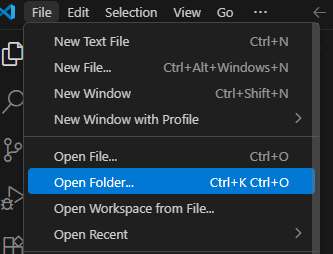
\includegraphics[keepaspectratio]{contents/app/assets/img/20250811124111.png}}

The folder already contains the project files and the environment files.
You may see them from the file explorer.

\pandocbounded{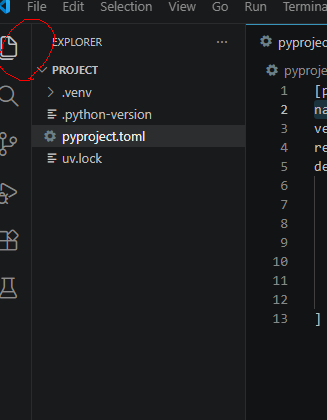
\includegraphics[keepaspectratio]{contents/app/assets/img/20260529132900.png}}

Then you may create new files/folders or copy files/folders into this
working folder. For demonstration a new file called
\texttt{helloworld.ipynb} is created.

\pandocbounded{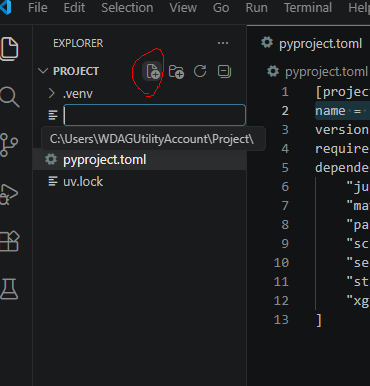
\includegraphics[keepaspectratio]{contents/app/assets/img/20260529133205.png}}

\texttt{ipynb} means this is a Jupyter notebook file (which is short for
\texttt{interactive\ Python\ notebook}). This is the format for this
course's homework assignment.

This is the appearance of an empty notebook file.

\pandocbounded{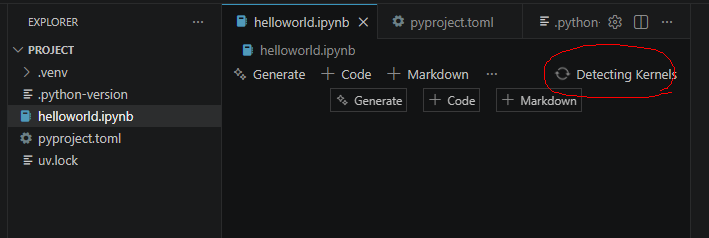
\includegraphics[keepaspectratio]{contents/app/assets/img/20260529133321.png}}

We attach the kernel we just created to this notebook. Click the
\texttt{Select\ Kernel} / \texttt{Detecting\ Kernels} on the right upper
corner and select the environment we want.

\pandocbounded{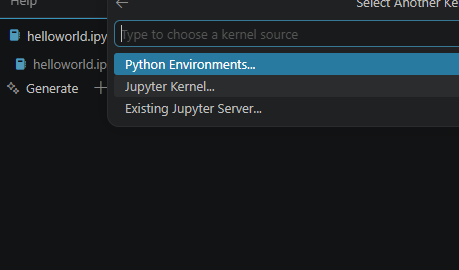
\includegraphics[keepaspectratio]{contents/app/assets/img/20260529150001.png}}

\begin{itemize}
\tightlist
\item
  If you created a new Jupyter kernel, you can find it from
  \texttt{Jupyter\ kernel...}.
\item
  If not, you can find your virtual environement in the working folder
  from \texttt{Python\ Environments...}.
\end{itemize}

\pandocbounded{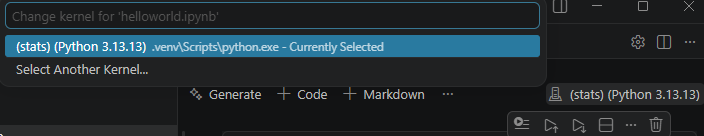
\includegraphics[keepaspectratio]{contents/app/assets/img/20260530232943.png}}

After the kernel is selected, we could start using the notebook. I
prefer to use the following code as hello world. It can also tell us
whether the correct python is used.

\begin{Shaded}
\begin{Highlighting}[]
\ImportTok{import}\NormalTok{ sys}
\BuiltInTok{print}\NormalTok{(sys.executable)}
\end{Highlighting}
\end{Shaded}

\pandocbounded{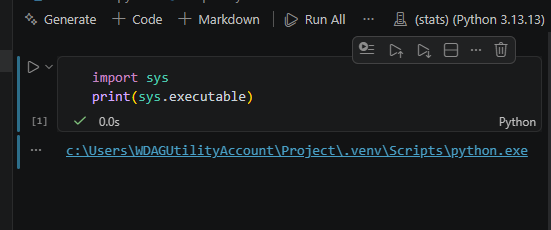
\includegraphics[keepaspectratio]{contents/app/assets/img/20260530233118.png}}

\subsection{Output to html and pdf}\label{output-to-html-and-pdf}

After finishing your Jupyter Notebook, you need to generate a PDF
version for assignment submission.

Since we do not want to spend too much time on document formatting, we
will use a simple workflow. Although there are many more sophisticated
tools available (such as Pandoc, Quarto, and LaTeX-based workflows), the
approach below is completely sufficient for this course.

Our workflow is:

\begin{enumerate}
\def\labelenumi{\arabic{enumi}.}
\setcounter{enumi}{-1}
\tightlist
\item
  Restart the kernel and run all.
\item
  Export the notebook to HTML using VS Code.
\item
  Open the HTML file in a web browser.
\item
  Print the page to a PDF file.
\end{enumerate}

First, locate the notebook toolbar and click the \texttt{...} button on
the right side. From the expanded menu, select \texttt{Export}.

\pandocbounded{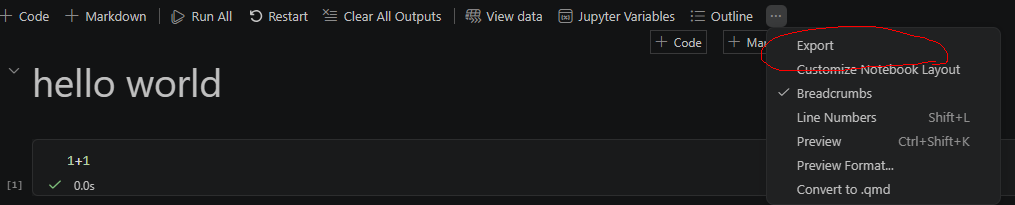
\includegraphics[keepaspectratio]{contents/app/assets/img/20260601211615.png}}

Then choose \texttt{HTML}.

\pandocbounded{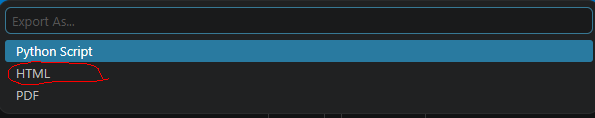
\includegraphics[keepaspectratio]{contents/app/assets/img/20260601211817.png}}

This will create an HTML file. Open the file in your preferred web
browser and print it to PDF. Most modern browsers (such as Chrome, Edge,
and Firefox) support printing directly to PDF.

For assignment submission, submit both the PDF file and the notebook
file. Grading will be based primarily on the PDF file, while the
notebook file serves as a backup source in case I need to inspect the
code or verify specific parts of the submission.

\begin{tcolorbox}[enhanced jigsaw, arc=.35mm, bottomrule=.15mm, bottomtitle=1mm, breakable, colback=white, colbacktitle=quarto-callout-note-color!10!white, colframe=quarto-callout-note-color-frame, coltitle=black, left=2mm, leftrule=.75mm, opacityback=0, opacitybacktitle=0.6, rightrule=.15mm, title=\textcolor{quarto-callout-note-color}{\faInfo}\hspace{0.5em}{Restart and Run All}, titlerule=0mm, toprule=.15mm, toptitle=1mm]

A Jupyter notebook keeps its internal state in memory while you work. As
a result, cells can be executed in different orders, making it possible
for the notebook contents and the actual execution state to become
inconsistent.

For example, a variable may exist because it was created in an earlier
session, even though the cell that creates it has been deleted and no
longer appears before its first use in the notebook. Such notebooks may
appear to run correctly during editing but fail when executed from
scratch.

To avoid these issues, you are required to restart the kernel and run
all cells before creating your submission PDF. Any errors that occur
during this process must be fixed before submission.

Although notebook workflows have several well-known limitations, Jupyter
notebooks remain the dominant platform for data science, machine
learning, and scientific computing. New alternatives such as
\texttt{marimo} have attracted considerable attention in recent years,
but they are still relatively young and may require several more years
to reach the level of adoption enjoyed by Jupyter --- if they ever do.

\end{tcolorbox}

\section{WSL}\label{sec-wsl}

WSL stands for Windows subsystem for Linux. It allows you to run a Linux
environment directly inside Windows without installing a separate
operating system.

To install WSL, please follow the
\href{https://learn.microsoft.com/en-us/windows/wsl/install}{official
Microsoft guide}.

After installation, you will have a Linux system (usually Ubuntu)
running alongside Windows. The Linux file system is separate from the
Windows file system, although you can access it through File Explorer to
copy / move files back and forth.

\pandocbounded{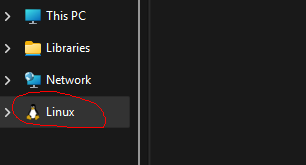
\includegraphics[keepaspectratio]{contents/app/assets/img/20260601170305.png}}

VS Code provides excellent support for WSL through the Remote WSL
extension. To open a WSL window, you may:

\begin{itemize}
\tightlist
\item
  Click the button in the lower-left corner of VS Code
  \pandocbounded{
\includegraphics[keepaspectratio]{contents/app/assets/img/20260601170444.png}}
\item
  Or open the Command Palette (\texttt{Ctrl+Shift+P} or \texttt{F1}),
  search for \texttt{WSL}, and select one of the available options. For
  most situations, \texttt{Connect\ to\ WSL\ in\ New\ Window} is the
  easiest choice.
  \pandocbounded{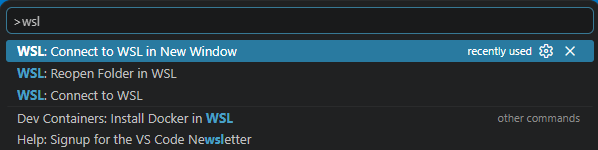
\includegraphics[keepaspectratio]{contents/app/assets/img/20260601170609.png}}
\end{itemize}

Once connected to WSL, you are working inside a Linux environment rather
than Windows.

Because WSL is a separate system, you will need to:

\begin{itemize}
\tightlist
\item
  Open your project folder again.
\item
  Install \texttt{uv}, Python and other tools inside WSL.
\item
  Create virtual environments inside WSL.
\item
  Install packages inside WSL.
\end{itemize}

You may follow the same instructions presented earlier to install
\texttt{uv} and set up your Python environment. The overall process is
the same, although the commands will be the Linux versions rather than
the Windows versions.

Note that if you install \texttt{uv} in Windows, it is not automatically
available inside WSL. Similarly, software installed inside WSL is
generally not available in Windows.

In practice, it is usually easiest to keep an entire project inside WSL
and perform all Python-related work there.

\begin{tcolorbox}[enhanced jigsaw, arc=.35mm, bottomrule=.15mm, bottomtitle=1mm, breakable, colback=white, colbacktitle=quarto-callout-tip-color!10!white, colframe=quarto-callout-tip-color-frame, coltitle=black, left=2mm, leftrule=.75mm, opacityback=0, opacitybacktitle=0.6, rightrule=.15mm, title=\textcolor{quarto-callout-tip-color}{\faLightbulb}\hspace{0.5em}{Tip}, titlerule=0mm, toprule=.15mm, toptitle=1mm]

Avoid storing virtual environments inside the Windows file system when
working primarily in WSL. For best performance and compatibility, create
your project folders inside your Linux home directory (for example,
\texttt{\textasciitilde{}/Project}) rather than in mounted Windows
directories (for example, \texttt{/mnt/c/...}).

\end{tcolorbox}

\chapter{Jupyter Notebook and
Markdown}\label{jupyter-notebook-and-markdown}

One of the best features of a Jupyter Notebook is that it can combine
code, narrative text, and output in a single file.

There are two types of cells in a notebook: Code cells and Markdown
cells.

\begin{itemize}
\tightlist
\item
  Code cells are used to run Python code.
\item
  Markdown cells are used to write text, explanations, equations, and
  documentation.
\end{itemize}

In statistical learning, code cells are typically used for data
analysis, model fitting, and computations, while Markdown cells are used
to explain the methods, interpret the results, and document the
workflow.

\pandocbounded{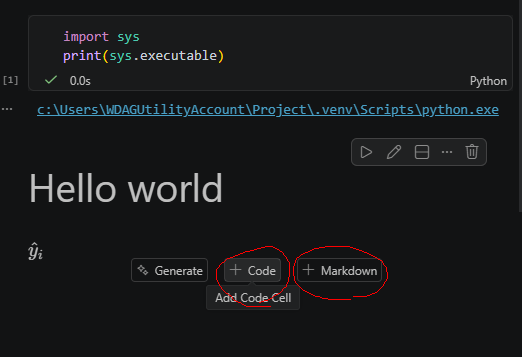
\includegraphics[keepaspectratio]{contents/app/assets/img/20260530234530.png}}

A notebook combines code, output, and narrative in a single document,
making it an ideal environment for data science and machine learning.

\begin{tcolorbox}[enhanced jigsaw, arc=.35mm, bottomrule=.15mm, bottomtitle=1mm, breakable, colback=white, colbacktitle=quarto-callout-tip-color!10!white, colframe=quarto-callout-tip-color-frame, coltitle=black, left=2mm, leftrule=.75mm, opacityback=0, opacitybacktitle=0.6, rightrule=.15mm, title=\textcolor{quarto-callout-tip-color}{\faLightbulb}\hspace{0.5em}{Tip}, titlerule=0mm, toprule=.15mm, toptitle=1mm]

You can always click the small \texttt{Edit} / \texttt{Stop\ Editing}
button to preview how your Markdown text will be rendered.

\end{tcolorbox}

\pandocbounded{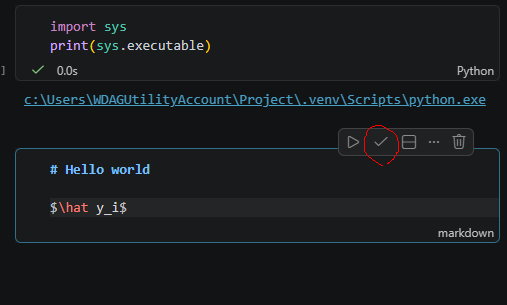
\includegraphics[keepaspectratio]{contents/app/assets/img/20260530233822.png}}

\pandocbounded{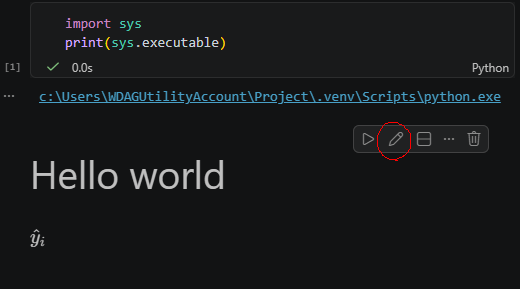
\includegraphics[keepaspectratio]{contents/app/assets/img/20260530233847.png}}

Markdown is a lightweight text format. In this course, we will use only
the most basic Markdown syntax.

\section{Text Formatting}\label{text-formatting}

{\def\LTcaptype{none} % do not increment counter
\begin{longtable}[]{@{}
  >{\raggedright\arraybackslash}p{(\linewidth - 2\tabcolsep) * \real{0.5000}}
  >{\raggedright\arraybackslash}p{(\linewidth - 2\tabcolsep) * \real{0.5000}}@{}}
\toprule\noalign{}
\begin{minipage}[b]{\linewidth}\raggedright
Markdown Syntax
\end{minipage} & \begin{minipage}[b]{\linewidth}\raggedright
Output
\end{minipage} \\
\midrule\noalign{}
\endhead
\bottomrule\noalign{}
\endlastfoot
\begin{minipage}[t]{\linewidth}\raggedright
\begin{Shaded}
\begin{Highlighting}[]
\NormalTok{*italics*, **bold**, ***bold italics***}
\end{Highlighting}
\end{Shaded}
\end{minipage} & \emph{italics}, \textbf{bold}, \textbf{\emph{bold
italics}} \\
\begin{minipage}[t]{\linewidth}\raggedright
\begin{Shaded}
\begin{Highlighting}[]
\NormalTok{\textasciitilde{}\textasciitilde{}strikethrough\textasciitilde{}\textasciitilde{}}
\end{Highlighting}
\end{Shaded}
\end{minipage} & \st{strikethrough} \\
\begin{minipage}[t]{\linewidth}\raggedright
\begin{Shaded}
\begin{Highlighting}[]
\InformationTok{\textasciigrave{}verbatim code\textasciigrave{}}
\end{Highlighting}
\end{Shaded}
\end{minipage} & \texttt{verbatim\ code} \\
\begin{minipage}[t]{\linewidth}\raggedright
\begin{Shaded}
\begin{Highlighting}[]
\InformationTok{\textasciigrave{}\textasciigrave{}\textasciigrave{}}
\InformationTok{multiline}
\InformationTok{code}
\InformationTok{\textasciigrave{}\textasciigrave{}\textasciigrave{}}
\end{Highlighting}
\end{Shaded}
\end{minipage} & \begin{minipage}[t]{\linewidth}\raggedright
\begin{verbatim}
multiple
code
\end{verbatim}
\end{minipage} \\
\end{longtable}
}

\section{Headings}\label{headings}

{\def\LTcaptype{none} % do not increment counter
\begin{longtable}[]{@{}ll@{}}
\toprule\noalign{}
Markdown Syntax & Output \\
\midrule\noalign{}
\endhead
\bottomrule\noalign{}
\endlastfoot
\texttt{\#\ Heading\ 1} & \(\Large\textbf{Heading 1}\) \\
\texttt{\#\#\ Heading\ 2} & \(\large\textbf{Heading 2}\) \\
\texttt{\#\#\#\ Heading\ 3} & \(\normalsize\textbf{Heading 3}\) \\
\end{longtable}
}

\begin{tcolorbox}[enhanced jigsaw, arc=.35mm, bottomrule=.15mm, bottomtitle=1mm, breakable, colback=white, colbacktitle=quarto-callout-tip-color!10!white, colframe=quarto-callout-tip-color-frame, coltitle=black, left=2mm, leftrule=.75mm, opacityback=0, opacitybacktitle=0.6, rightrule=.15mm, title=\textcolor{quarto-callout-tip-color}{\faLightbulb}\hspace{0.5em}{Tip}, titlerule=0mm, toprule=.15mm, toptitle=1mm]

Note that for heading, there is a space after \texttt{\#}.

\end{tcolorbox}

\section{Lists}\label{lists}

{\def\LTcaptype{none} % do not increment counter
\begin{longtable}[]{@{}
  >{\raggedright\arraybackslash}p{(\linewidth - 2\tabcolsep) * \real{0.5000}}
  >{\raggedright\arraybackslash}p{(\linewidth - 2\tabcolsep) * \real{0.5000}}@{}}
\toprule\noalign{}
\begin{minipage}[b]{\linewidth}\raggedright
Markdown Syntax
\end{minipage} & \begin{minipage}[b]{\linewidth}\raggedright
Output
\end{minipage} \\
\midrule\noalign{}
\endhead
\bottomrule\noalign{}
\endlastfoot
\begin{minipage}[t]{\linewidth}\raggedright
\begin{Shaded}
\begin{Highlighting}[]
\SpecialStringTok{* }\NormalTok{unordered list}
\SpecialStringTok{  + }\NormalTok{sub{-}item 1}
\SpecialStringTok{  + }\NormalTok{sub{-}item 2}
\SpecialStringTok{    {-} }\NormalTok{sub{-}sub{-}item 1}
\end{Highlighting}
\end{Shaded}
\end{minipage} & \begin{minipage}[t]{\linewidth}\raggedright
\begin{itemize}
\tightlist
\item
  unordered list

  \begin{itemize}
  \tightlist
  \item
    sub-item 1
  \item
    sub-item 2

    \begin{itemize}
    \tightlist
    \item
      sub-sub-item 1
    \end{itemize}
  \end{itemize}
\end{itemize}
\end{minipage} \\
\begin{minipage}[t]{\linewidth}\raggedright
\begin{Shaded}
\begin{Highlighting}[]
\SpecialStringTok{1. }\NormalTok{ordered list}
\SpecialStringTok{2. }\NormalTok{item 2}
\NormalTok{   i) sub{-}item 1}
\NormalTok{      A.  sub{-}sub{-}item 1}
\end{Highlighting}
\end{Shaded}
\end{minipage} & \begin{minipage}[t]{\linewidth}\raggedright
\begin{enumerate}
\def\labelenumi{\arabic{enumi}.}
\tightlist
\item
  ordered list
\item
  item 2

  \begin{enumerate}
  \def\labelenumii{\roman{enumii})}
  \tightlist
  \item
    sub-item 1

    \begin{enumerate}
    \def\labelenumiii{\Alph{enumiii}.}
    \tightlist
    \item
      sub-sub-item 1
    \end{enumerate}
  \end{enumerate}
\end{enumerate}
\end{minipage} \\
\end{longtable}
}

\begin{tcolorbox}[enhanced jigsaw, arc=.35mm, bottomrule=.15mm, bottomtitle=1mm, breakable, colback=white, colbacktitle=quarto-callout-tip-color!10!white, colframe=quarto-callout-tip-color-frame, coltitle=black, left=2mm, leftrule=.75mm, opacityback=0, opacitybacktitle=0.6, rightrule=.15mm, title=\textcolor{quarto-callout-tip-color}{\faLightbulb}\hspace{0.5em}{Tip}, titlerule=0mm, toprule=.15mm, toptitle=1mm]

Note that for lists, there is a space after \texttt{.}.

\end{tcolorbox}

\section{Essential LaTeX}\label{essential-latex}

Use single dollar signs for inline math:

\begin{Shaded}
\begin{Highlighting}[]
\NormalTok{The fitted value is $\textbackslash{}hat y\_i$.}
\end{Highlighting}
\end{Shaded}

\begin{quote}
The fitted value is \(\hat y_i\).
\end{quote}

Use double dollar signs for displayed equations:

\begin{Shaded}
\begin{Highlighting}[]
\NormalTok{$$}
\NormalTok{Y = \textbackslash{}beta\_0 + \textbackslash{}beta\_1 X + \textbackslash{}epsilon.}
\NormalTok{$$}
\end{Highlighting}
\end{Shaded}

\[
Y = \beta_0 + \beta_1 X + \epsilon.
\]

Common symbols:

\begin{Shaded}
\begin{Highlighting}[]
\NormalTok{$\textbackslash{}hat y$        predicted value}
\NormalTok{$\textbackslash{}bar x$        sample mean}
\NormalTok{$\textbackslash{}beta\_0$       parameter}
\NormalTok{$X\^{}\textbackslash{}top X$      transpose}
\NormalTok{$\textbackslash{}sum\_\{i=1\}\^{}n$  summation}
\end{Highlighting}
\end{Shaded}

\begin{quote}
\(\hat y\): predicted value

\(\bar x\): sample mean

\(\beta_0\): parameter

\(X^\top X\): transpose

\(\sum_{i=1}^n\): summation
\end{quote}

LaTeX supports a wide range of mathematical notation, but the basic
symbols introduced here will be enough for all of the work in this
course.

\chapter{\texorpdfstring{Python Basics for
\texttt{sklearn}}{Python Basics for sklearn}}\label{python-basics-for-sklearn}

This note introduces only the Python syntax needed for the rest of these
notes. The goal is not to cover Python as a full programming language.
The goal is to make code using \texttt{numpy}, \texttt{matplotlib}, and
\texttt{sklearn} readable.

\section{Running Python Code}\label{running-python-code}

A Python code chunk looks like this:

\begin{Shaded}
\begin{Highlighting}[]
\CommentTok{\# This is a comment}

\NormalTok{x }\OperatorTok{=} \DecValTok{10}      \CommentTok{\# assignment uses =}

\NormalTok{a, b }\OperatorTok{=} \DecValTok{2}\NormalTok{, }\DecValTok{3}
\NormalTok{a }\OperatorTok{+}\NormalTok{ b       }\CommentTok{\# last expression is automatically displayed}
\end{Highlighting}
\end{Shaded}

\begin{verbatim}
5
\end{verbatim}

\begin{tcolorbox}[enhanced jigsaw, arc=.35mm, bottomrule=.15mm, bottomtitle=1mm, breakable, colback=white, colbacktitle=quarto-callout-tip-color!10!white, colframe=quarto-callout-tip-color-frame, coltitle=black, left=2mm, leftrule=.75mm, opacityback=0, opacitybacktitle=0.6, rightrule=.15mm, title=\textcolor{quarto-callout-tip-color}{\faLightbulb}\hspace{0.5em}{Tip}, titlerule=0mm, toprule=.15mm, toptitle=1mm]

In Python power operation is \texttt{**}. Therefore \texttt{3**2} is
\texttt{9}.

\end{tcolorbox}

\begin{tcolorbox}[enhanced jigsaw, arc=.35mm, bottomrule=.15mm, bottomtitle=1mm, breakable, colback=white, colbacktitle=quarto-callout-note-color!10!white, colframe=quarto-callout-note-color-frame, coltitle=black, left=2mm, leftrule=.75mm, opacityback=0, opacitybacktitle=0.6, rightrule=.15mm, title=\textcolor{quarto-callout-note-color}{\faInfo}\hspace{0.5em}{Notebook}, titlerule=0mm, toprule=.15mm, toptitle=1mm]

\begin{enumerate}
\def\labelenumi{\arabic{enumi}.}
\item
  When a code cell is executed, the value of the last expression is
  automatically displayed. Any explicit output commands, such as
  \texttt{print()}, will also produce output.
\item
  Use \texttt{\#} comments only for short notes that help explain the
  code. Detailed explanations and discussion should be written in
  Markdown cells, where they are easier to read and maintain.
\end{enumerate}

\end{tcolorbox}

\subsection{Indentation}\label{indentation}

Python uses indentation to mark code blocks. R uses braces
\texttt{\{\}}; Python uses indentation.

For example, a \texttt{for} loop:

\begin{Shaded}
\begin{Highlighting}[]
\ControlFlowTok{for}\NormalTok{ k }\KeywordTok{in}\NormalTok{ [}\DecValTok{1}\NormalTok{, }\DecValTok{3}\NormalTok{, }\DecValTok{5}\NormalTok{]:}
    \BuiltInTok{print}\NormalTok{(k)}
\end{Highlighting}
\end{Shaded}

\begin{verbatim}
1
3
5
\end{verbatim}

The indented block belongs to the loop. These notes use loops only when
they are helpful for plotting or comparing models.

\subsection{\texorpdfstring{\texttt{if} and
\texttt{for}}{if and for}}\label{if-and-for}

The logic of \texttt{if} statements and \texttt{for} loops is
straightforward. When using them, pay attention to indentation. A colon
\texttt{:} indicates the beginning of an indented code block.

\begin{Shaded}
\begin{Highlighting}[]
\NormalTok{x }\OperatorTok{=} \DecValTok{1}
\ControlFlowTok{if}\NormalTok{ x }\OperatorTok{==} \DecValTok{2}\NormalTok{:}
    \BuiltInTok{print}\NormalTok{(}\StringTok{\textquotesingle{}good\textquotesingle{}}\NormalTok{)}
\ControlFlowTok{else}\NormalTok{:}
    \BuiltInTok{print}\NormalTok{(}\StringTok{\textquotesingle{}not good\textquotesingle{}}\NormalTok{)}
\end{Highlighting}
\end{Shaded}

\begin{verbatim}
not good
\end{verbatim}

\begin{Shaded}
\begin{Highlighting}[]
\ControlFlowTok{for}\NormalTok{ k }\KeywordTok{in} \BuiltInTok{range}\NormalTok{(}\DecValTok{4}\NormalTok{):}
    \BuiltInTok{print}\NormalTok{(k)}
\end{Highlighting}
\end{Shaded}

\begin{verbatim}
0
1
2
3
\end{verbatim}

\begin{Shaded}
\begin{Highlighting}[]
\ControlFlowTok{for}\NormalTok{ val }\KeywordTok{in}\NormalTok{ [}\StringTok{\textquotesingle{}a\textquotesingle{}}\NormalTok{, }\StringTok{\textquotesingle{}b\textquotesingle{}}\NormalTok{, }\DecValTok{1}\NormalTok{, }\DecValTok{3}\NormalTok{]:}
    \BuiltInTok{print}\NormalTok{(val)}
\end{Highlighting}
\end{Shaded}

\begin{verbatim}
a
b
1
3
\end{verbatim}

\subsection{Functions and Objects}\label{functions-and-objects}

This is not an object-oriented programming course, so don't worry too
much about the details. The important idea is the distinction between a
function, a class, and an object created from a class.

\begin{itemize}
\tightlist
\item
  Function: performs an action and returns a result. Called with
  parentheses: \texttt{round(3.14,\ 2)}
\item
  Class: a blueprint for creating objects.
\item
  Object: stores information and provides methods. Accessed with a dot:
  \texttt{object.method()}
\end{itemize}

Example in scikit-learn:

\begin{Shaded}
\begin{Highlighting}[]
\NormalTok{model }\OperatorTok{=}\NormalTok{ LinearRegression()}
\end{Highlighting}
\end{Shaded}

Here

\begin{itemize}
\tightlist
\item
  \texttt{LinearRegression} is the class;
\item
  \texttt{LinearRegression()} creates a linear regression model object;
\item
  the object is assigned to the variable \texttt{model}.
\end{itemize}

\begin{Shaded}
\begin{Highlighting}[]
\NormalTok{model.fit(X\_train, y\_train)}
\NormalTok{coef }\OperatorTok{=}\NormalTok{ model.coef\_}
\end{Highlighting}
\end{Shaded}

Here

\begin{itemize}
\tightlist
\item
  \texttt{fit()} is method;
\item
  \texttt{coef\_} stores information about the fitted model;
\item
  methods are called using \texttt{object.method(...)};
\item
  stored information is accessed using \texttt{object.attribute}.
\end{itemize}

In almost all \texttt{scikit-learn} code, you should work with objects
rather than classes. A common mistake is to pass a class where an object
is required.

\begin{Shaded}
\begin{Highlighting}[]
\NormalTok{pipe }\OperatorTok{=}\NormalTok{ make\_pipeline(StandardScaler, LinearRegression)     }\CommentTok{\# wrong}
\NormalTok{pipe }\OperatorTok{=}\NormalTok{ make\_pipeline(StandardScaler(), LinearRegression()) }\CommentTok{\# correct}
\end{Highlighting}
\end{Shaded}

The same idea applies to most \texttt{scikit-learn} components,
including transformers, models, and pipelines. In general, if something
is used as a step in a pipeline, you should create an object by adding
\texttt{()}.

\begin{tcolorbox}[enhanced jigsaw, arc=.35mm, bottomrule=.15mm, bottomtitle=1mm, breakable, colback=white, colbacktitle=quarto-callout-caution-color!10!white, colframe=quarto-callout-caution-color-frame, coltitle=black, left=2mm, leftrule=.75mm, opacityback=0, opacitybacktitle=0.6, rightrule=.15mm, title=\textcolor{quarto-callout-caution-color}{\faFire}\hspace{0.5em}{\texttt{.} (Dot)}, titlerule=0mm, toprule=.15mm, toptitle=1mm]

The meaning of \texttt{.} is different in Python and R.

\begin{itemize}
\tightlist
\item
  In Python, \texttt{.} is used to access methods and attributes of an
  object.
\end{itemize}

\begin{Shaded}
\begin{Highlighting}[]
\NormalTok{model.fit(X, y)}
\NormalTok{model.coef\_}
\end{Highlighting}
\end{Shaded}

\begin{itemize}
\tightlist
\item
  In R, \texttt{.} is usually just part of a variable or function name.
\end{itemize}

\begin{Shaded}
\begin{Highlighting}[]
\NormalTok{my.variable }\OtherTok{\textless{}{-}} \DecValTok{1}
\end{Highlighting}
\end{Shaded}

Do not interpret dots in R names as object access.

\end{tcolorbox}

\subsection{Importing Packages}\label{importing-packages}

Python packages are loaded with \texttt{import}.

The usual imports in these notes are:

\begin{Shaded}
\begin{Highlighting}[]
\ImportTok{import}\NormalTok{ numpy }\ImportTok{as}\NormalTok{ np}
\ImportTok{import}\NormalTok{ pandas }\ImportTok{as}\NormalTok{ pd}
\ImportTok{import}\NormalTok{ matplotlib.pyplot }\ImportTok{as}\NormalTok{ plt}
\end{Highlighting}
\end{Shaded}

The names on the right are aliases:

\begin{itemize}
\tightlist
\item
  \texttt{numpy} is used as \texttt{np};
\item
  \texttt{pandas} is used as \texttt{pd};
\item
  \texttt{matplotlib.pyplot} is used as \texttt{plt}.
\end{itemize}

After importing a package this way, you access its functions using the
package name, e.g.

\begin{itemize}
\tightlist
\item
  \texttt{np.array({[}1,\ 2,\ 3{]})}
\item
  \texttt{pd.DataFrame(\{"x":\ {[}1,\ 2,\ 3{]}\})}
\item
  \texttt{plt.plot({[}1,\ 2,\ 3{]},\ {[}4,\ 5,\ 6{]})}
\end{itemize}

\begin{tcolorbox}[enhanced jigsaw, arc=.35mm, bottomrule=.15mm, bottomtitle=1mm, breakable, colback=white, colbacktitle=quarto-callout-note-color!10!white, colframe=quarto-callout-note-color-frame, coltitle=black, left=2mm, leftrule=.75mm, opacityback=0, opacitybacktitle=0.6, rightrule=.15mm, title=\textcolor{quarto-callout-note-color}{\faInfo}\hspace{0.5em}{Note}, titlerule=0mm, toprule=.15mm, toptitle=1mm]

When a package is imported with \texttt{import\ ...\ as\ ...}, you must
use the alias to access its functions and classes instead of the
original name.

\end{tcolorbox}

Sometimes only specific functions or classes are imported.

\begin{Shaded}
\begin{Highlighting}[]
\ImportTok{from}\NormalTok{ sklearn.linear\_model }\ImportTok{import}\NormalTok{ LinearRegression}
\ImportTok{from}\NormalTok{ sklearn.model\_selection }\ImportTok{import}\NormalTok{ train\_test\_split}
\end{Highlighting}
\end{Shaded}

These objects can then be used directly.

\begin{Shaded}
\begin{Highlighting}[]
\NormalTok{model }\OperatorTok{=}\NormalTok{ LinearRegression()}
\end{Highlighting}
\end{Shaded}

\begin{tcolorbox}[enhanced jigsaw, arc=.35mm, bottomrule=.15mm, bottomtitle=1mm, breakable, colback=white, colbacktitle=quarto-callout-note-color!10!white, colframe=quarto-callout-note-color-frame, coltitle=black, left=2mm, leftrule=.75mm, opacityback=0, opacitybacktitle=0.6, rightrule=.15mm, title=\textcolor{quarto-callout-note-color}{\faInfo}\hspace{0.5em}{Note}, titlerule=0mm, toprule=.15mm, toptitle=1mm]

After \texttt{from\ sklearn.linear\_model\ import\ LinearRegression},
you may use \texttt{LinearRegression()} directly, but other objects from
\texttt{sklearn.linear\_model} are not automatically imported.

\end{tcolorbox}

\section{Data structure}\label{data-structure}

\subsection{Basic Objects}\label{basic-objects}

Python has several basic data types.

\begin{Shaded}
\begin{Highlighting}[]
\NormalTok{x }\OperatorTok{=} \DecValTok{3}          \CommentTok{\# integer}
\NormalTok{y }\OperatorTok{=} \FloatTok{2.5}        \CommentTok{\# float}
\NormalTok{name }\OperatorTok{=} \StringTok{"tree"}  \CommentTok{\# string}
\NormalTok{flag }\OperatorTok{=} \VariableTok{True}    \CommentTok{\# Boolean}
\end{Highlighting}
\end{Shaded}

Use \texttt{type()} to check the type of an object.

\begin{Shaded}
\begin{Highlighting}[]
\BuiltInTok{type}\NormalTok{(y)}
\end{Highlighting}
\end{Shaded}

\begin{verbatim}
float
\end{verbatim}

Python is case-sensitive. \texttt{x} and \texttt{X} are different
objects.

\subsection{Lists}\label{lists-1}

A list is an \textbf{ordered collection} of objects. Lists are commonly
used to store variable names, column names, or collections of parameter
values.

{\def\LTcaptype{none} % do not increment counter
\begin{longtable}[]{@{}
  >{\raggedright\arraybackslash}p{(\linewidth - 4\tabcolsep) * \real{0.1890}}
  >{\raggedright\arraybackslash}p{(\linewidth - 4\tabcolsep) * \real{0.3386}}
  >{\raggedright\arraybackslash}p{(\linewidth - 4\tabcolsep) * \real{0.4724}}@{}}
\toprule\noalign{}
\begin{minipage}[b]{\linewidth}\raggedright
Purpose
\end{minipage} & \begin{minipage}[b]{\linewidth}\raggedright
Example
\end{minipage} & \begin{minipage}[b]{\linewidth}\raggedright
Explanation
\end{minipage} \\
\midrule\noalign{}
\endhead
\bottomrule\noalign{}
\endlastfoot
Create a list &
\texttt{features\ =\ {[}"age",\ "income",\ "education"{]}} & Creates a
list containing three strings. \\
Access the first element & \texttt{features{[}0{]}} & Returns
\texttt{"age"}. Python indexing starts at \texttt{0}. \\
Access the last element & \texttt{features{[}-1{]}} & Returns
\texttt{"education"}. Negative indices count from the end. \\
Select several elements & \texttt{features{[}0:2{]}} & Returns
\texttt{{[}"age",\ "income"{]}}. The stop index is not included. \\
Add an element & \texttt{features.append("gender")} & Adds
\texttt{"gender"} to the end of the list. \\
Count elements & \texttt{len(features)} & Returns the number of elements
in the list. \\
\end{longtable}
}

\begin{tcolorbox}[enhanced jigsaw, arc=.35mm, bottomrule=.15mm, bottomtitle=1mm, breakable, colback=white, colbacktitle=quarto-callout-note-color!10!white, colframe=quarto-callout-note-color-frame, coltitle=black, left=2mm, leftrule=.75mm, opacityback=0, opacitybacktitle=0.6, rightrule=.15mm, title=\textcolor{quarto-callout-note-color}{\faInfo}\hspace{0.5em}{Note}, titlerule=0mm, toprule=.15mm, toptitle=1mm]

Unlike R, Python uses zero-based indexing, so the first element has
index \texttt{0}.

\end{tcolorbox}

\subsection{Dictionaries}\label{dictionaries}

A dictionary stores \textbf{key-value pairs}. It is similar to a named
list in R and is commonly used to store settings, options, and model
parameters.

{\def\LTcaptype{none} % do not increment counter
\begin{longtable}[]{@{}
  >{\raggedright\arraybackslash}p{(\linewidth - 4\tabcolsep) * \real{0.1680}}
  >{\raggedright\arraybackslash}p{(\linewidth - 4\tabcolsep) * \real{0.4080}}
  >{\raggedright\arraybackslash}p{(\linewidth - 4\tabcolsep) * \real{0.4240}}@{}}
\toprule\noalign{}
\begin{minipage}[b]{\linewidth}\raggedright
Purpose
\end{minipage} & \begin{minipage}[b]{\linewidth}\raggedright
Example
\end{minipage} & \begin{minipage}[b]{\linewidth}\raggedright
Explanation
\end{minipage} \\
\midrule\noalign{}
\endhead
\bottomrule\noalign{}
\endlastfoot
Create a dictionary &
\texttt{params\ =\ \{"n\_neighbors":\ 5,\ "weights":\ "uniform"\}} &
Creates a dictionary with two keys and their values. \\
Access a value & \texttt{params{[}"n\_neighbors"{]}} & Returns
\texttt{5}. \\
Add or update a value & \texttt{params{[}"metric"{]}\ =\ "euclidean"} &
Adds a new key-value pair or updates an existing one. \\
Count entries & \texttt{len(params)} & Returns the number of key-value
pairs. \\
Store model settings &
\texttt{\{"max\_depth":\ 3,\ "min\_samples\_leaf":\ 5\}} & A common use
in machine learning. \\
Store parameter grids & \texttt{\{"max\_depth":\ {[}2,3,4{]}\}} & Often
used when tuning hyperparameters. \\
\end{longtable}
}

A typical parameter grid in \texttt{scikit-learn} looks like:

\begin{Shaded}
\begin{Highlighting}[]
\NormalTok{param\_grid }\OperatorTok{=}\NormalTok{ \{}
    \StringTok{"max\_depth"}\NormalTok{: [}\DecValTok{2}\NormalTok{, }\DecValTok{3}\NormalTok{, }\DecValTok{4}\NormalTok{],}
    \StringTok{"min\_samples\_leaf"}\NormalTok{: [}\DecValTok{1}\NormalTok{, }\DecValTok{5}\NormalTok{, }\DecValTok{10}\NormalTok{],}
\NormalTok{\}}
\end{Highlighting}
\end{Shaded}

For pipelines, parameter names often use two underscores:

\begin{Shaded}
\begin{Highlighting}[]
\NormalTok{param\_grid }\OperatorTok{=}\NormalTok{ \{}
    \StringTok{"model\_\_C"}\NormalTok{: [}\FloatTok{0.1}\NormalTok{, }\DecValTok{1}\NormalTok{, }\DecValTok{10}\NormalTok{],}
\NormalTok{\}}
\end{Highlighting}
\end{Shaded}

\begin{tcolorbox}[enhanced jigsaw, arc=.35mm, bottomrule=.15mm, bottomtitle=1mm, breakable, colback=white, colbacktitle=quarto-callout-note-color!10!white, colframe=quarto-callout-note-color-frame, coltitle=black, left=2mm, leftrule=.75mm, opacityback=0, opacitybacktitle=0.6, rightrule=.15mm, title=\textcolor{quarto-callout-note-color}{\faInfo}\hspace{0.5em}{Note}, titlerule=0mm, toprule=.15mm, toptitle=1mm]

In a pipeline, a parameter name of the form \texttt{step\_\_parameter}
refers to a parameter inside a specific pipeline step. For example,
\texttt{model\_\_C} means the parameter \texttt{C} of the pipeline step
named \texttt{"model"}. More terminologies will be discussed in related
sections.

\end{tcolorbox}

\section{\texorpdfstring{\texttt{numpy.array}}{numpy.array}}\label{numpy.array}

The most important data structure for numerical computation in Python is
\texttt{numpy.array}.

\begin{Shaded}
\begin{Highlighting}[]
\ImportTok{import}\NormalTok{ numpy }\ImportTok{as}\NormalTok{ np}

\NormalTok{x }\OperatorTok{=}\NormalTok{ np.array([}\DecValTok{1}\NormalTok{, }\DecValTok{2}\NormalTok{, }\DecValTok{3}\NormalTok{, }\DecValTok{4}\NormalTok{])}
\NormalTok{x}
\end{Highlighting}
\end{Shaded}

\begin{verbatim}
array([1, 2, 3, 4])
\end{verbatim}

Arrays have a shape and a dimension.

\begin{Shaded}
\begin{Highlighting}[]
\BuiltInTok{print}\NormalTok{(x.shape)}
\BuiltInTok{print}\NormalTok{(x.ndim)}
\end{Highlighting}
\end{Shaded}

\begin{verbatim}
(4,)
1
\end{verbatim}

So \texttt{x} is a 1D array containing 4 elements.

\subsection{2D Arrays}\label{d-arrays}

A 2D array is similar to a matrix.

\begin{Shaded}
\begin{Highlighting}[]
\NormalTok{X }\OperatorTok{=}\NormalTok{ np.array([}
\NormalTok{    [}\DecValTok{1}\NormalTok{, }\DecValTok{2}\NormalTok{],}
\NormalTok{    [}\DecValTok{3}\NormalTok{, }\DecValTok{4}\NormalTok{],}
\NormalTok{    [}\DecValTok{5}\NormalTok{, }\DecValTok{6}\NormalTok{]}
\NormalTok{])}

\NormalTok{X}
\end{Highlighting}
\end{Shaded}

\begin{verbatim}
array([[1, 2],
       [3, 4],
       [5, 6]])
\end{verbatim}

\begin{Shaded}
\begin{Highlighting}[]
\BuiltInTok{print}\NormalTok{(X.shape)}
\BuiltInTok{print}\NormalTok{(X.ndim)}
\end{Highlighting}
\end{Shaded}

\begin{verbatim}
(3, 2)
2
\end{verbatim}

Here \texttt{X} is a 2D array with 3 rows and 2 columns.

\subsection{Indexing}\label{indexing}

Use \texttt{{[}row,\ column{]}} indexing.

\begin{Shaded}
\begin{Highlighting}[]
\NormalTok{X[}\DecValTok{0}\NormalTok{, }\DecValTok{1}\NormalTok{]      }\CommentTok{\# row 0, column 1}
\NormalTok{X[:, }\DecValTok{0}\NormalTok{]      }\CommentTok{\# first column}
\NormalTok{X[}\DecValTok{1}\NormalTok{, :]      }\CommentTok{\# second row}
\end{Highlighting}
\end{Shaded}

The symbol \texttt{:} means ``all indices'' along that axis.

Slicing can select ranges.

\begin{Shaded}
\begin{Highlighting}[]
\NormalTok{X[}\DecValTok{0}\NormalTok{:}\DecValTok{2}\NormalTok{, }\DecValTok{1}\NormalTok{]      }\CommentTok{\# first 2 rows, column 1}
\NormalTok{X[}\DecValTok{0}\NormalTok{, }\DecValTok{0}\NormalTok{:}\DecValTok{2}\NormalTok{]      }\CommentTok{\# row 0, first 2 columns}
\NormalTok{X[}\DecValTok{0}\NormalTok{:}\DecValTok{2}\NormalTok{, }\DecValTok{0}\NormalTok{:}\DecValTok{2}\NormalTok{]    }\CommentTok{\# upper{-}left 2x2 block}
\end{Highlighting}
\end{Shaded}

\begin{tcolorbox}[enhanced jigsaw, arc=.35mm, bottomrule=.15mm, bottomtitle=1mm, breakable, colback=white, colbacktitle=quarto-callout-note-color!10!white, colframe=quarto-callout-note-color-frame, coltitle=black, left=2mm, leftrule=.75mm, opacityback=0, opacitybacktitle=0.6, rightrule=.15mm, title=\textcolor{quarto-callout-note-color}{\faInfo}\hspace{0.5em}{Note}, titlerule=0mm, toprule=.15mm, toptitle=1mm]

\texttt{X{[}:,\ 0{]}} returns a 1D array with shape \texttt{(n,)}, not a
column vector.

To obtain a column vector, use

\begin{Shaded}
\begin{Highlighting}[]
\NormalTok{X[:, [}\DecValTok{0}\NormalTok{]]}
\CommentTok{\# or}
\NormalTok{X[:, }\DecValTok{0}\NormalTok{].reshape(}\OperatorTok{{-}}\DecValTok{1}\NormalTok{, }\DecValTok{1}\NormalTok{)}
\end{Highlighting}
\end{Shaded}

which both have shape \texttt{(n,\ 1)}.

\end{tcolorbox}

\subsection{Common Operations}\label{sec-common_operations}

Arrays support vectorized arithmetic.

\begin{Shaded}
\begin{Highlighting}[]
\NormalTok{x }\OperatorTok{+} \DecValTok{1}
\NormalTok{x }\OperatorTok{*} \DecValTok{2}
\NormalTok{np.mean(x)}
\end{Highlighting}
\end{Shaded}

Operations are applied elementwise.

There are two special operations that is worth mentioning.

\begin{tcolorbox}[enhanced jigsaw, arc=.35mm, bottomrule=.15mm, bottomtitle=1mm, breakable, colback=white, colbacktitle=quarto-callout-note-color!10!white, colframe=quarto-callout-note-color-frame, coltitle=black, left=2mm, leftrule=.75mm, opacityback=0, opacitybacktitle=0.6, rightrule=.15mm, title=\textcolor{quarto-callout-note-color}{\faInfo}\hspace{0.5em}{Matrix multiplication}, titlerule=0mm, toprule=.15mm, toptitle=1mm]

There are several ways to perform matrix multiplication in NumPy. Here
we introduce the \texttt{@} operator because it has the simplest syntax.

\begin{Shaded}
\begin{Highlighting}[]
\ImportTok{import}\NormalTok{ numpy }\ImportTok{as}\NormalTok{ np}

\NormalTok{X }\OperatorTok{=}\NormalTok{ np.array([[}\DecValTok{1}\NormalTok{, }\DecValTok{2}\NormalTok{], [}\DecValTok{3}\NormalTok{, }\DecValTok{4}\NormalTok{], [}\DecValTok{5}\NormalTok{, }\DecValTok{6}\NormalTok{]])}
\NormalTok{y }\OperatorTok{=}\NormalTok{ np.array([}\DecValTok{1}\NormalTok{, }\DecValTok{2}\NormalTok{])}
\NormalTok{X }\OperatorTok{@}\NormalTok{ y}
\end{Highlighting}
\end{Shaded}

\begin{verbatim}
array([ 5, 11, 17])
\end{verbatim}

\begin{Shaded}
\begin{Highlighting}[]
\NormalTok{X }\OperatorTok{=}\NormalTok{ np.array([[}\DecValTok{1}\NormalTok{, }\DecValTok{2}\NormalTok{], [}\DecValTok{3}\NormalTok{, }\DecValTok{4}\NormalTok{], [}\DecValTok{5}\NormalTok{, }\DecValTok{6}\NormalTok{]])}
\NormalTok{y }\OperatorTok{=}\NormalTok{ np.array([}\DecValTok{1}\NormalTok{, }\DecValTok{2}\NormalTok{]).reshape(}\OperatorTok{{-}}\DecValTok{1}\NormalTok{, }\DecValTok{1}\NormalTok{)}
\NormalTok{X }\OperatorTok{@}\NormalTok{ y}
\end{Highlighting}
\end{Shaded}

\begin{verbatim}
array([[ 5],
       [11],
       [17]])
\end{verbatim}

Note that the result depends on the dimensions of the inputs. NumPy
automatically applies the appropriate matrix multiplication rule based
on the shapes of the arrays.

\begin{itemize}
\tightlist
\item
  In the first example, \texttt{y} is a one-dimensional array with shape
  \texttt{(2,)}, so the result is also one-dimensional with shape
  \texttt{(3,)}.
\item
  In the second example, \texttt{y} is a column vector with shape
  \texttt{(2,1)}, so the result is a two-dimensional array with shape
  \texttt{(3,1)}.
\end{itemize}

\end{tcolorbox}

\begin{tcolorbox}[enhanced jigsaw, arc=.35mm, bottomrule=.15mm, bottomtitle=1mm, breakable, colback=white, colbacktitle=quarto-callout-note-color!10!white, colframe=quarto-callout-note-color-frame, coltitle=black, left=2mm, leftrule=.75mm, opacityback=0, opacitybacktitle=0.6, rightrule=.15mm, title=\textcolor{quarto-callout-note-color}{\faInfo}\hspace{0.5em}{Broadcasting}, titlerule=0mm, toprule=.15mm, toptitle=1mm]

Broadcasting is a NumPy mechanism that allows arithmetic operations
between arrays of different shapes.

Instead of explicitly copying data, NumPy automatically expands arrays
along dimensions of size 1 when the shapes are compatible. Two
dimensions are compatible if they are equal or if one of them is 1.

A common example is arithmetic between an array and a scalar:

\begin{Shaded}
\begin{Highlighting}[]
\ImportTok{import}\NormalTok{ numpy }\ImportTok{as}\NormalTok{ np}

\NormalTok{X }\OperatorTok{=}\NormalTok{ np.array([[}\DecValTok{1}\NormalTok{, }\DecValTok{2}\NormalTok{], [}\DecValTok{3}\NormalTok{, }\DecValTok{4}\NormalTok{], [}\DecValTok{5}\NormalTok{, }\DecValTok{6}\NormalTok{]])}
\NormalTok{X }\OperatorTok{+} \DecValTok{10}
\end{Highlighting}
\end{Shaded}

\begin{verbatim}
array([[11, 12],
       [13, 14],
       [15, 16]])
\end{verbatim}

The scalar is automatically applied to every element of the array.

Broadcasting can also occur between higher-dimensional arrays. For
example,

\begin{Shaded}
\begin{Highlighting}[]
\NormalTok{a }\OperatorTok{=}\NormalTok{ np.array([[}\DecValTok{1}\NormalTok{, }\DecValTok{2}\NormalTok{, }\DecValTok{3}\NormalTok{]]) }
\NormalTok{b }\OperatorTok{=}\NormalTok{ np.array([[}\DecValTok{10}\NormalTok{], [}\DecValTok{20}\NormalTok{]])}
\NormalTok{a }\OperatorTok{+}\NormalTok{ b}
\end{Highlighting}
\end{Shaded}

\begin{verbatim}
array([[11, 12, 13],
       [21, 22, 23]])
\end{verbatim}

Here \texttt{a} has shape \texttt{(1,3)} and \texttt{b} has shape
\texttt{(2,1)}. These shapes are compatible because, along each axis,
either the dimensions are equal or one of them is \texttt{1}.

Broadcasting expands dimensions of size \texttt{1} to match the
corresponding dimension of the other array. In this example, the single
row of \texttt{a} behaves as if it were repeated twice, while the single
column of \texttt{b} behaves as if it were repeated three times,
resulting in arrays of shape \texttt{(2,3)}.

Broadcasting can also be used to compute pairwise differences
efficiently.

\begin{Shaded}
\begin{Highlighting}[]
\ImportTok{import}\NormalTok{ numpy }\ImportTok{as}\NormalTok{ np}

\NormalTok{X1 }\OperatorTok{=}\NormalTok{ np.array([[}\DecValTok{1}\NormalTok{, }\DecValTok{2}\NormalTok{],}
\NormalTok{               [}\DecValTok{3}\NormalTok{, }\DecValTok{4}\NormalTok{]])}

\NormalTok{X2 }\OperatorTok{=}\NormalTok{ np.array([[}\DecValTok{1}\NormalTok{, }\DecValTok{2}\NormalTok{],}
\NormalTok{               [}\DecValTok{3}\NormalTok{, }\DecValTok{4}\NormalTok{]])}

\NormalTok{d }\OperatorTok{=}\NormalTok{ X1[:, }\VariableTok{None}\NormalTok{] }\OperatorTok{{-}}\NormalTok{ X2[}\VariableTok{None}\NormalTok{, :]}
\NormalTok{d}
\end{Highlighting}
\end{Shaded}

\begin{verbatim}
array([[[ 0,  0],
        [-2, -2]],

       [[ 2,  2],
        [ 0,  0]]])
\end{verbatim}

\texttt{None} inserts a new dimension at the specified location.
Therefore \texttt{X1{[}:,\ None{]}} has shape \texttt{(2,1,2)} while
\texttt{X2{[}None,\ :{]}} has shape \texttt{(1,2,2)}.

NumPy automatically broadcasts these arrays to shape
\texttt{(2,\ 2,\ 2)} and computes all pairwise differences at once.

In this example, each row of \texttt{X1} is subtracted from each row of
\texttt{X2}. The result satisfies
\texttt{d{[}i,\ j{]}\ =\ X1{[}i{]}\ -\ X2{[}j{]}} for all valid indices
\texttt{i} and \texttt{j}.

This technique is frequently used when computing distance matrices in
machine learning algorithms.

\end{tcolorbox}

\subsection{Axis-wise}\label{axis-wise}

Many functions accept an \texttt{axis=} argument.

\begin{Shaded}
\begin{Highlighting}[]
\NormalTok{X              }\CommentTok{\# show X}
\end{Highlighting}
\end{Shaded}

\begin{verbatim}
array([[1, 2],
       [3, 4],
       [5, 6]])
\end{verbatim}

Computes the sum across rows:

\begin{Shaded}
\begin{Highlighting}[]
\NormalTok{X.}\BuiltInTok{sum}\NormalTok{(axis}\OperatorTok{=}\DecValTok{0}\NormalTok{)}
\end{Highlighting}
\end{Shaded}

\begin{verbatim}
array([ 9, 12])
\end{verbatim}

Computes the mean across columns:

\begin{Shaded}
\begin{Highlighting}[]
\NormalTok{X.mean(axis}\OperatorTok{=}\DecValTok{1}\NormalTok{)}
\end{Highlighting}
\end{Shaded}

\begin{verbatim}
array([1.5, 3.5, 5.5])
\end{verbatim}

A useful rule:

\begin{itemize}
\tightlist
\item
  \texttt{axis=0}: operate down rows (one result per column)
\item
  \texttt{axis=1}: operate across columns (one result per row)
\end{itemize}

\subsection{Reshaping}\label{reshaping}

A 1D array can be converted into a matrix. Consider a 1D array

\begin{Shaded}
\begin{Highlighting}[]
\NormalTok{x }\OperatorTok{=}\NormalTok{ np.array([}\DecValTok{1}\NormalTok{, }\DecValTok{2}\NormalTok{, }\DecValTok{3}\NormalTok{, }\DecValTok{4}\NormalTok{])}
\end{Highlighting}
\end{Shaded}

To create a column vector:

\begin{Shaded}
\begin{Highlighting}[]
\NormalTok{x.reshape(}\OperatorTok{{-}}\DecValTok{1}\NormalTok{, }\DecValTok{1}\NormalTok{)}
\end{Highlighting}
\end{Shaded}

\begin{verbatim}
array([[1],
       [2],
       [3],
       [4]])
\end{verbatim}

To create a row vector:

\begin{Shaded}
\begin{Highlighting}[]
\NormalTok{x.reshape(}\DecValTok{1}\NormalTok{, }\OperatorTok{{-}}\DecValTok{1}\NormalTok{)}
\end{Highlighting}
\end{Shaded}

\begin{verbatim}
array([[1, 2, 3, 4]])
\end{verbatim}

The value \texttt{-1} means ``infer this dimension automatically.''

A common pattern is

\begin{Shaded}
\begin{Highlighting}[]
\NormalTok{test\_x }\OperatorTok{=}\NormalTok{ np.linspace(}\DecValTok{0}\NormalTok{, }\DecValTok{1}\NormalTok{, }\DecValTok{101}\NormalTok{).reshape(}\OperatorTok{{-}}\DecValTok{1}\NormalTok{, }\DecValTok{1}\NormalTok{)}
\end{Highlighting}
\end{Shaded}

On the other side, to flatten an array back to 1D:

\begin{Shaded}
\begin{Highlighting}[]
\NormalTok{X.reshape(}\OperatorTok{{-}}\DecValTok{1}\NormalTok{)}
\end{Highlighting}
\end{Shaded}

\begin{verbatim}
array([1, 2, 3, 4, 5, 6])
\end{verbatim}

\texttt{NumPy} reads entries row by row and produces a one-dimensional
array.

\begin{tcolorbox}[enhanced jigsaw, arc=.35mm, bottomrule=.15mm, bottomtitle=1mm, breakable, colback=white, colbacktitle=quarto-callout-tip-color!10!white, colframe=quarto-callout-tip-color-frame, coltitle=black, left=2mm, leftrule=.75mm, opacityback=0, opacitybacktitle=0.6, rightrule=.15mm, title=\textcolor{quarto-callout-tip-color}{\faLightbulb}\hspace{0.5em}{Tip}, titlerule=0mm, toprule=.15mm, toptitle=1mm]

Other flattening methods include \texttt{.ravel()} and
\texttt{.flatten()}. The difference is about how copy-and-view is
handled. We mainly use \texttt{.reshape(-1)} because it makes the
resulting shape explicit.

\end{tcolorbox}

\begin{tcolorbox}[enhanced jigsaw, arc=.35mm, bottomrule=.15mm, bottomtitle=1mm, breakable, colback=white, colbacktitle=quarto-callout-note-color!10!white, colframe=quarto-callout-note-color-frame, coltitle=black, left=2mm, leftrule=.75mm, opacityback=0, opacitybacktitle=0.6, rightrule=.15mm, title=\textcolor{quarto-callout-note-color}{\faInfo}\hspace{0.5em}{Note}, titlerule=0mm, toprule=.15mm, toptitle=1mm]

One common source of bugs in statistical learning is using arrays with
incorrect shapes.

In \texttt{scikit-learn}, predictors \texttt{X} are usually stored as a
2D array and responses \texttt{y} as a 1D array. Other libraries may use
different conventions, and the required shapes often depend on the
specific model or loss function.

When shape-related errors occur, always check the documentation of the
library you are using.

\end{tcolorbox}

\subsection{Arrays versus Lists}\label{arrays-versus-lists}

Lists are general-purpose containers, and its addition concatenates. For
example

\begin{Shaded}
\begin{Highlighting}[]
\NormalTok{[}\DecValTok{1}\NormalTok{, }\DecValTok{2}\NormalTok{, }\DecValTok{3}\NormalTok{] }\OperatorTok{+}\NormalTok{ [}\DecValTok{4}\NormalTok{, }\DecValTok{5}\NormalTok{, }\DecValTok{6}\NormalTok{]}
\end{Highlighting}
\end{Shaded}

\begin{verbatim}
[1, 2, 3, 4, 5, 6]
\end{verbatim}

Arrays are designed for numerical computation. Its operations are align
with the regular math operations. Therefore for numerical work and
machine learning, use \texttt{numpy.array} whenever possible.

\section{Random Numbers}\label{random-numbers}

These notes often use \texttt{numpy} random number generators for
simulation.

\begin{Shaded}
\begin{Highlighting}[]
\NormalTok{rng }\OperatorTok{=}\NormalTok{ np.random.default\_rng(}\DecValTok{1}\NormalTok{)}

\NormalTok{x }\OperatorTok{=}\NormalTok{ rng.normal(size}\OperatorTok{=}\DecValTok{5}\NormalTok{)}
\NormalTok{x}
\end{Highlighting}
\end{Shaded}

\begin{verbatim}
array([ 0.34558419,  0.82161814,  0.33043708, -1.30315723,  0.90535587])
\end{verbatim}

\begin{tcolorbox}[enhanced jigsaw, arc=.35mm, bottomrule=.15mm, bottomtitle=1mm, breakable, colback=white, colbacktitle=quarto-callout-note-color!10!white, colframe=quarto-callout-note-color-frame, coltitle=black, left=2mm, leftrule=.75mm, opacityback=0, opacitybacktitle=0.6, rightrule=.15mm, title=\textcolor{quarto-callout-note-color}{\faInfo}\hspace{0.5em}{Note}, titlerule=0mm, toprule=.15mm, toptitle=1mm]

The number \texttt{1} is a seed. It makes the random output
reproducible.

On a single machine, if the seed is fixed the results are supposed to be
the same.

You may choose any number as the seed. You may use the same seed when
you want to see the same result.

\end{tcolorbox}

Some common random functions are:

\begin{Shaded}
\begin{Highlighting}[]
\NormalTok{rng.normal(loc}\OperatorTok{=}\DecValTok{0}\NormalTok{, scale}\OperatorTok{=}\DecValTok{1}\NormalTok{, size}\OperatorTok{=}\DecValTok{5}\NormalTok{)}
\end{Highlighting}
\end{Shaded}

\begin{verbatim}
array([ 0.44637457, -0.53695324,  0.5811181 ,  0.3645724 ,  0.2941325 ])
\end{verbatim}

\begin{Shaded}
\begin{Highlighting}[]
\NormalTok{rng.uniform(}\DecValTok{0}\NormalTok{, }\DecValTok{1}\NormalTok{, size}\OperatorTok{=}\DecValTok{5}\NormalTok{)}
\end{Highlighting}
\end{Shaded}

\begin{verbatim}
array([0.75351311, 0.53814331, 0.32973172, 0.7884287 , 0.30319483])
\end{verbatim}

For a two-dimensional predictor matrix:

\begin{Shaded}
\begin{Highlighting}[]
\NormalTok{X }\OperatorTok{=}\NormalTok{ rng.normal(size}\OperatorTok{=}\NormalTok{(}\DecValTok{10}\NormalTok{, }\DecValTok{3}\NormalTok{))}
\NormalTok{X.shape}
\end{Highlighting}
\end{Shaded}

\begin{verbatim}
(10, 3)
\end{verbatim}

\section{\texorpdfstring{\texttt{pandas}}{pandas}}\label{pandas}

\texttt{pandas} can be treated as a wrapper of \texttt{numpy.array}
which make it more readable. The complete \texttt{pandas} is very
complicated. Here we only mention a few very important concepts.

To import \texttt{pandas}, in most cases we set \texttt{pd} as its
alias.

\begin{Shaded}
\begin{Highlighting}[]
\ImportTok{import}\NormalTok{ pandas }\ImportTok{as}\NormalTok{ pd}
\end{Highlighting}
\end{Shaded}

\subsection{\texorpdfstring{\texttt{DataFrame} and
\texttt{Series}}{DataFrame and Series}}\label{dataframe-and-series}

In \texttt{pandas}, \texttt{DataFrame} is the 2D data table, and
\texttt{Series} is the 1D column. There are many ways to create a
\texttt{DataFrame}. Here we focus on one of them, that is to convert a
\texttt{dict} into a \texttt{DataFrame}.

\begin{Shaded}
\begin{Highlighting}[]
\NormalTok{results }\OperatorTok{=}\NormalTok{ \{}
    \StringTok{\textquotesingle{}round\textquotesingle{}}\NormalTok{: [}\DecValTok{1}\NormalTok{, }\DecValTok{2}\NormalTok{, }\DecValTok{3}\NormalTok{, }\DecValTok{4}\NormalTok{, }\DecValTok{5}\NormalTok{],}
    \StringTok{\textquotesingle{}score\textquotesingle{}}\NormalTok{: [}\FloatTok{0.22}\NormalTok{, }\FloatTok{0.33}\NormalTok{, }\FloatTok{0.44}\NormalTok{, }\FloatTok{0.55}\NormalTok{, }\FloatTok{0.66}\NormalTok{], }
    \StringTok{\textquotesingle{}mse\textquotesingle{}}\NormalTok{: [}\FloatTok{0.12}\NormalTok{, }\FloatTok{0.11}\NormalTok{, }\FloatTok{0.10}\NormalTok{, }\FloatTok{0.09}\NormalTok{, }\FloatTok{0.08}\NormalTok{]}
\NormalTok{\}}
\NormalTok{df\_res }\OperatorTok{=}\NormalTok{ pd.DataFrame(results)}
\NormalTok{df\_res}
\end{Highlighting}
\end{Shaded}

{\def\LTcaptype{none} % do not increment counter
\begin{longtable}[]{@{}llll@{}}
\toprule\noalign{}
& round & score & mse \\
\midrule\noalign{}
\endhead
\bottomrule\noalign{}
\endlastfoot
0 & 1 & 0.22 & 0.12 \\
1 & 2 & 0.33 & 0.11 \\
2 & 3 & 0.44 & 0.10 \\
3 & 4 & 0.55 & 0.09 \\
4 & 5 & 0.66 & 0.08 \\
\end{longtable}
}

A single column is returned as a \texttt{Series}.

\begin{Shaded}
\begin{Highlighting}[]
\NormalTok{df\_res[}\StringTok{\textquotesingle{}score\textquotesingle{}}\NormalTok{]}
\end{Highlighting}
\end{Shaded}

\begin{verbatim}
0    0.22
1    0.33
2    0.44
3    0.55
4    0.66
Name: score, dtype: float64
\end{verbatim}

Notice that this is similar to \texttt{numpy} indexing. Selecting a
single column by name returns a 1D object. If we instead pass a list of
column names, even if the list contains only one column
(e.g.~\texttt{{[}\textquotesingle{}score\textquotesingle{}{]}} below),
the result is a 2D \texttt{DataFrame}.

\begin{Shaded}
\begin{Highlighting}[]
\NormalTok{df\_res[[}\StringTok{\textquotesingle{}score\textquotesingle{}}\NormalTok{]]}
\end{Highlighting}
\end{Shaded}

{\def\LTcaptype{none} % do not increment counter
\begin{longtable}[]{@{}ll@{}}
\toprule\noalign{}
& score \\
\midrule\noalign{}
\endhead
\bottomrule\noalign{}
\endlastfoot
0 & 0.22 \\
1 & 0.33 \\
2 & 0.44 \\
3 & 0.55 \\
4 & 0.66 \\
\end{longtable}
}

This behavior is analogous to the difference between
\texttt{X{[}:,\ 0{]}} and \texttt{X{[}:,\ {[}0{]}{]}} for a
\texttt{numpy} array:

\begin{itemize}
\tightlist
\item
  \texttt{df\_res{[}"score"{]}} returns a \texttt{Series} (1D)
\item
  \texttt{df\_res{[}{[}"score"{]}{]}} returns a \texttt{DataFrame} (2D)
\item
  \texttt{X{[}:,\ 0{]}} returns a 1D array
\item
  \texttt{X{[}:,\ {[}0{]}{]}} returns a 2D array
\end{itemize}

\subsection{Read and write files}\label{read-and-write-files}

In \texttt{scikit-learn}, predictors and responses can be stored either
as \texttt{numpy} arrays or as \texttt{pandas} objects. Throughout this
course, many examples use \texttt{numpy}, but most code works equally
well with \texttt{pandas} data structures.

When working with external datasets, a common workflow is:

\begin{enumerate}
\def\labelenumi{\arabic{enumi}.}
\tightlist
\item
  Read the data into a \texttt{DataFrame}.
\item
  Perform data cleaning and preprocessing.
\item
  Extract predictors and responses.
\item
  Fit a statistical learning model.
\end{enumerate}

Two of the most common tabular file formats are CSV files and Excel
spreadsheets.

\begin{tcolorbox}[enhanced jigsaw, arc=.35mm, bottomrule=.15mm, bottomtitle=1mm, breakable, colback=white, colbacktitle=quarto-callout-note-color!10!white, colframe=quarto-callout-note-color-frame, coltitle=black, left=2mm, leftrule=.75mm, opacityback=0, opacitybacktitle=0.6, rightrule=.15mm, title=\textcolor{quarto-callout-note-color}{\faInfo}\hspace{0.5em}{CSV}, titlerule=0mm, toprule=.15mm, toptitle=1mm]

CSV stands for comma-separated values. A CSV file is a plain-text file
that stores tabular data using a separator between columns.

Common separators include:

\begin{itemize}
\tightlist
\item
  \texttt{,} (comma)
\item
  \texttt{;} (semicolon)
\item
  \texttt{\textbackslash{}t} (tab)
\end{itemize}

Consider the following file \href{example.csv}{\texttt{example.csv}}.

\begin{verbatim}
round   score   mse
1   0.220000    0.120000
2   0.330000    0.110000
3   0.440000    0.100000
4   0.550000    0.090000
5   0.660000    0.080000
\end{verbatim}

In Python we could use \texttt{pd.read\_csv()} to read it.

\begin{Shaded}
\begin{Highlighting}[]
\ImportTok{import}\NormalTok{ pandas }\ImportTok{as}\NormalTok{ pd}
\NormalTok{df }\OperatorTok{=}\NormalTok{ pd.read\_csv(}\StringTok{\textquotesingle{}example.csv\textquotesingle{}}\NormalTok{)}
\NormalTok{df}
\end{Highlighting}
\end{Shaded}

{\def\LTcaptype{none} % do not increment counter
\begin{longtable}[]{@{}ll@{}}
\toprule\noalign{}
& round\textbackslash tscore\textbackslash tmse \\
\midrule\noalign{}
\endhead
\bottomrule\noalign{}
\endlastfoot
0 & 1\textbackslash t0.220000\textbackslash t0.120000 \\
1 & 2\textbackslash t0.330000\textbackslash t0.110000 \\
2 & 3\textbackslash t0.440000\textbackslash t0.100000 \\
3 & 4\textbackslash t0.550000\textbackslash t0.090000 \\
4 & 5\textbackslash t0.660000\textbackslash t0.080000 \\
\end{longtable}
}

The result is incorrect because this file uses tab characters
(\texttt{\textbackslash{}t}) rather than commas as separators.

Specify the separator explicitly:

\begin{Shaded}
\begin{Highlighting}[]
\NormalTok{df }\OperatorTok{=}\NormalTok{ pd.read\_csv(}\StringTok{\textquotesingle{}example.csv\textquotesingle{}}\NormalTok{, sep}\OperatorTok{=}\StringTok{\textquotesingle{}}\CharTok{\textbackslash{}t}\StringTok{\textquotesingle{}}\NormalTok{)}
\NormalTok{df}
\end{Highlighting}
\end{Shaded}

{\def\LTcaptype{none} % do not increment counter
\begin{longtable}[]{@{}llll@{}}
\toprule\noalign{}
& round & score & mse \\
\midrule\noalign{}
\endhead
\bottomrule\noalign{}
\endlastfoot
0 & 1 & 0.22 & 0.12 \\
1 & 2 & 0.33 & 0.11 \\
2 & 3 & 0.44 & 0.10 \\
3 & 4 & 0.55 & 0.09 \\
4 & 5 & 0.66 & 0.08 \\
\end{longtable}
}

\end{tcolorbox}

\begin{tcolorbox}[enhanced jigsaw, arc=.35mm, bottomrule=.15mm, bottomtitle=1mm, breakable, colback=white, colbacktitle=quarto-callout-note-color!10!white, colframe=quarto-callout-note-color-frame, coltitle=black, left=2mm, leftrule=.75mm, opacityback=0, opacitybacktitle=0.6, rightrule=.15mm, title=\textcolor{quarto-callout-note-color}{\faInfo}\hspace{0.5em}{Excel}, titlerule=0mm, toprule=.15mm, toptitle=1mm]

Excel spreadsheets can be read using \texttt{pd.read\_excel()}. We
provide the \href{example.xlsx}{\texttt{exmaple.xlsx}} as an example.

\begin{Shaded}
\begin{Highlighting}[]
\ImportTok{import}\NormalTok{ pandas }\ImportTok{as}\NormalTok{ pd}
\NormalTok{df }\OperatorTok{=}\NormalTok{ pd.read\_excel(}\StringTok{\textquotesingle{}example.xlsx\textquotesingle{}}\NormalTok{)}
\NormalTok{df}
\end{Highlighting}
\end{Shaded}

{\def\LTcaptype{none} % do not increment counter
\begin{longtable}[]{@{}llll@{}}
\toprule\noalign{}
& round & score & mse \\
\midrule\noalign{}
\endhead
\bottomrule\noalign{}
\endlastfoot
0 & 1 & 0.22 & 0.12 \\
1 & 2 & 0.33 & 0.11 \\
2 & 3 & 0.44 & 0.10 \\
3 & 4 & 0.55 & 0.09 \\
4 & 5 & 0.66 & 0.08 \\
\end{longtable}
}

Unlike CSV files, Excel files are stored in a binary format. Therefore,
\texttt{pandas} requires an additional package called an engine to read
and write them. The most commonly used engine is \texttt{openpyxl}.

\begin{Shaded}
\begin{Highlighting}[]
\ExtensionTok{uv}\NormalTok{ add openpyxl}
\end{Highlighting}
\end{Shaded}

Although not provided in the toml file, \texttt{openpyxl} was added to
our environment as an example in the introduction. If you didn't add it
at that time you may add it now.

\end{tcolorbox}

Writing files is similar to reading files. The main difference is that
writing starts from an existing \texttt{DataFrame} instead of starting
from \texttt{pd}.

\begin{Shaded}
\begin{Highlighting}[]
\NormalTok{df.to\_csv(}\StringTok{\textquotesingle{}example2.csv\textquotesingle{}}\NormalTok{)}
\NormalTok{df.to\_excel(}\StringTok{\textquotesingle{}example2.xlsx\textquotesingle{}}\NormalTok{)}
\end{Highlighting}
\end{Shaded}

\subsection{Relative paths}\label{relative-paths}

In this course, always use relative paths when reading or writing files.

A relative path starts from the current working directory rather than
from the root of the file system.

Suppose your working directory is

\begin{Shaded}
\begin{Highlighting}[]
\NormalTok{C:/Users/WDAGUtilityAccount/Project/}
\end{Highlighting}
\end{Shaded}

and you have the following structure:

\begin{Shaded}
\begin{Highlighting}[]
\NormalTok{Project/}
\NormalTok{├── example.csv}
\NormalTok{└── foldername/}
\end{Highlighting}
\end{Shaded}

Then you can read and write files using:

\begin{Shaded}
\begin{Highlighting}[]
\NormalTok{df }\OperatorTok{=}\NormalTok{ pd.read\_csv(}\StringTok{"example.csv"}\NormalTok{)}
\NormalTok{df.to\_csv(}\StringTok{"foldername/result.csv"}\NormalTok{)}
\end{Highlighting}
\end{Shaded}

Notice that neither path begins with a drive name such as \texttt{C:} or
\texttt{D:}.

If your files are stored outside the working directory, \textbf{copy
them into the working directory} before reading them.

\begin{tcolorbox}[enhanced jigsaw, arc=.35mm, bottomrule=.15mm, bottomtitle=1mm, breakable, colback=white, colbacktitle=quarto-callout-note-color!10!white, colframe=quarto-callout-note-color-frame, coltitle=black, left=2mm, leftrule=.75mm, opacityback=0, opacitybacktitle=0.6, rightrule=.15mm, title=\textcolor{quarto-callout-note-color}{\faInfo}\hspace{0.5em}{Note}, titlerule=0mm, toprule=.15mm, toptitle=1mm]

Although absolute paths such as

\begin{Shaded}
\begin{Highlighting}[]
\NormalTok{pd.read\_csv(}\StringTok{"D:/Files/example.csv"}\NormalTok{)}
\end{Highlighting}
\end{Shaded}

often work on your own computer, they may fail on another computer
because the file locations are different.

Using relative paths makes your code more portable and easier to share.

\end{tcolorbox}

\section{\texorpdfstring{\texttt{matplotlib}
Basics}{matplotlib Basics}}\label{matplotlib-basics}

These notes use only basic \texttt{matplotlib}. The standard import is:

\begin{Shaded}
\begin{Highlighting}[]
\ImportTok{import}\NormalTok{ matplotlib.pyplot }\ImportTok{as}\NormalTok{ plt}
\end{Highlighting}
\end{Shaded}

We provide some code examples here. Most of the commands are
straightforward. Please check the
\href{https://matplotlib.org/}{official document} if you need more
details.

\subsection{Scatter Plot}\label{scatter-plot}

\begin{Shaded}
\begin{Highlighting}[]
\NormalTok{x }\OperatorTok{=}\NormalTok{ np.array([}\DecValTok{1}\NormalTok{, }\DecValTok{2}\NormalTok{, }\DecValTok{3}\NormalTok{, }\DecValTok{4}\NormalTok{])}
\NormalTok{y }\OperatorTok{=}\NormalTok{ np.array([}\FloatTok{1.1}\NormalTok{, }\FloatTok{2.0}\NormalTok{, }\FloatTok{2.8}\NormalTok{, }\FloatTok{4.2}\NormalTok{])}

\NormalTok{plt.scatter(x, y)}
\NormalTok{plt.xlabel(}\StringTok{"x"}\NormalTok{)}
\NormalTok{plt.ylabel(}\StringTok{"y"}\NormalTok{)}
\NormalTok{plt.title(}\StringTok{"Scatter Plot"}\NormalTok{)}\OperatorTok{;}
\end{Highlighting}
\end{Shaded}

\pandocbounded{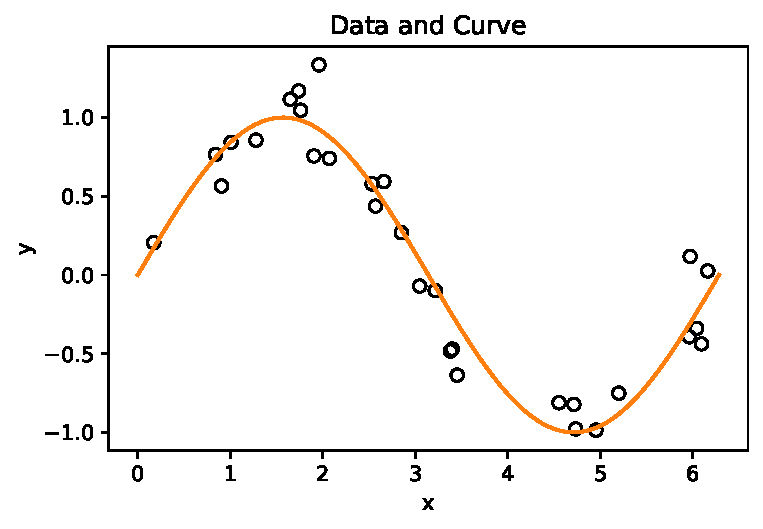
\includegraphics[keepaspectratio]{contents/app/python_files/figure-pdf/cell-46-output-1.pdf}}

\subsection{Line Plot}\label{line-plot}

\begin{Shaded}
\begin{Highlighting}[]
\NormalTok{x\_grid }\OperatorTok{=}\NormalTok{ np.linspace(}\DecValTok{0}\NormalTok{, }\DecValTok{2} \OperatorTok{*}\NormalTok{ np.pi, }\DecValTok{200}\NormalTok{)}
\NormalTok{y\_grid }\OperatorTok{=}\NormalTok{ np.sin(x\_grid)}

\NormalTok{plt.plot(x\_grid, y\_grid)}
\NormalTok{plt.xlabel(}\StringTok{"x"}\NormalTok{)}
\NormalTok{plt.ylabel(}\StringTok{"sin(x)"}\NormalTok{)}
\NormalTok{plt.title(}\StringTok{"Line Plot"}\NormalTok{)}\OperatorTok{;}
\end{Highlighting}
\end{Shaded}

\pandocbounded{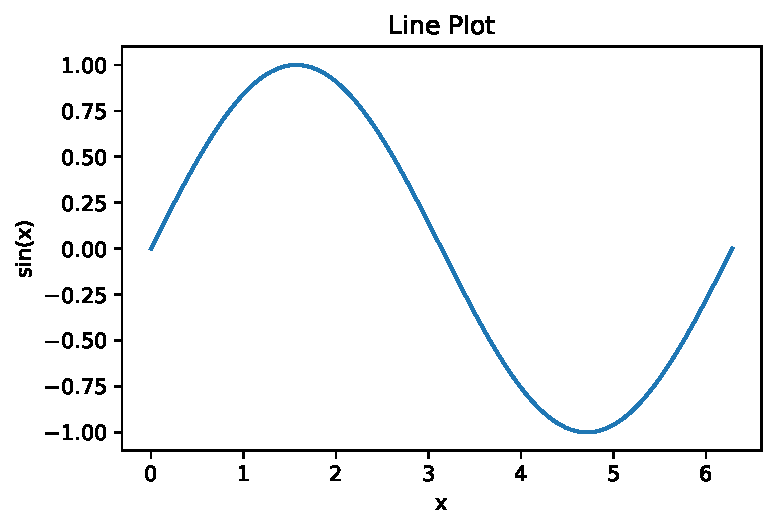
\includegraphics[keepaspectratio]{contents/app/python_files/figure-pdf/cell-47-output-1.pdf}}

\subsection{Scatter and Line Together}\label{scatter-and-line-together}

\begin{Shaded}
\begin{Highlighting}[]
\NormalTok{rng }\OperatorTok{=}\NormalTok{ np.random.default\_rng(}\DecValTok{1}\NormalTok{)}

\NormalTok{x }\OperatorTok{=}\NormalTok{ rng.uniform(}\DecValTok{0}\NormalTok{, }\DecValTok{2} \OperatorTok{*}\NormalTok{ np.pi, size}\OperatorTok{=}\DecValTok{30}\NormalTok{)}
\NormalTok{y }\OperatorTok{=}\NormalTok{ np.sin(x) }\OperatorTok{+}\NormalTok{ rng.normal(scale}\OperatorTok{=}\FloatTok{0.2}\NormalTok{, size}\OperatorTok{=}\DecValTok{30}\NormalTok{)}
\NormalTok{x\_grid }\OperatorTok{=}\NormalTok{ np.linspace(}\DecValTok{0}\NormalTok{, }\DecValTok{2} \OperatorTok{*}\NormalTok{ np.pi, }\DecValTok{200}\NormalTok{)}

\NormalTok{plt.scatter(x, y, facecolors}\OperatorTok{=}\StringTok{"none"}\NormalTok{, edgecolors}\OperatorTok{=}\StringTok{"black"}\NormalTok{)}
\NormalTok{plt.plot(x\_grid, np.sin(x\_grid), color}\OperatorTok{=}\StringTok{"C1"}\NormalTok{)}
\NormalTok{plt.xlabel(}\StringTok{"x"}\NormalTok{)}
\NormalTok{plt.ylabel(}\StringTok{"y"}\NormalTok{)}
\NormalTok{plt.title(}\StringTok{"Data and Curve"}\NormalTok{)}\OperatorTok{;}
\end{Highlighting}
\end{Shaded}

\pandocbounded{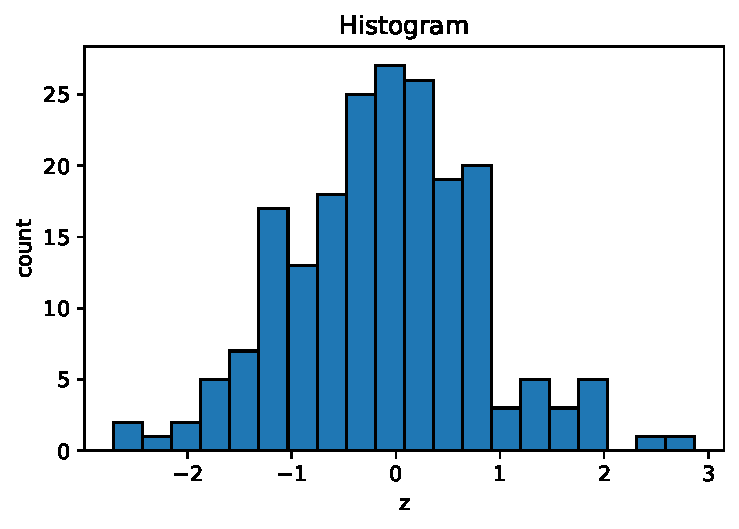
\includegraphics[keepaspectratio]{contents/app/python_files/figure-pdf/cell-48-output-1.pdf}}

This pattern appears often when we plot data points and a fitted curve.

\subsection{Multiple Plots}\label{multiple-plots}

Use \texttt{plt.subplots} for multiple panels.

\begin{Shaded}
\begin{Highlighting}[]
\NormalTok{fig, axs }\OperatorTok{=}\NormalTok{ plt.subplots(}\DecValTok{1}\NormalTok{, }\DecValTok{2}\NormalTok{, figsize}\OperatorTok{=}\NormalTok{(}\DecValTok{10}\NormalTok{, }\DecValTok{4}\NormalTok{))}

\NormalTok{axs[}\DecValTok{0}\NormalTok{].scatter(x, y)}
\NormalTok{axs[}\DecValTok{0}\NormalTok{].set\_title(}\StringTok{"scatter"}\NormalTok{)}

\NormalTok{axs[}\DecValTok{1}\NormalTok{].plot(x\_grid, np.sin(x\_grid))}
\NormalTok{axs[}\DecValTok{1}\NormalTok{].set\_title(}\StringTok{"line"}\NormalTok{)}\OperatorTok{;}
\end{Highlighting}
\end{Shaded}

\pandocbounded{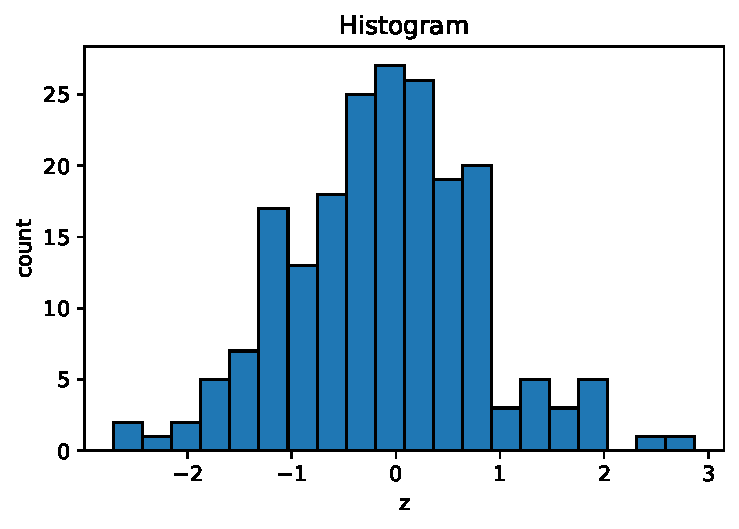
\includegraphics[keepaspectratio]{contents/app/python_files/figure-pdf/cell-49-output-1.pdf}}

\begin{tcolorbox}[enhanced jigsaw, arc=.35mm, bottomrule=.15mm, bottomtitle=1mm, breakable, colback=white, colbacktitle=quarto-callout-note-color!10!white, colframe=quarto-callout-note-color-frame, coltitle=black, left=2mm, leftrule=.75mm, opacityback=0, opacitybacktitle=0.6, rightrule=.15mm, title=\textcolor{quarto-callout-note-color}{\faInfo}\hspace{0.5em}{Note}, titlerule=0mm, toprule=.15mm, toptitle=1mm]

Notice that when using an axes object, many plotting commands have
different names. For example, \texttt{plt.title()} becomes
\texttt{ax.set\_title()}. Therefore, you cannot always replace
\texttt{plt} with \texttt{ax} directly. For details, consult the
official documentation.

\end{tcolorbox}

\subsection{Histograms}\label{histograms}

\begin{Shaded}
\begin{Highlighting}[]
\NormalTok{z }\OperatorTok{=}\NormalTok{ rng.normal(size}\OperatorTok{=}\DecValTok{200}\NormalTok{)}

\NormalTok{plt.hist(z, bins}\OperatorTok{=}\DecValTok{20}\NormalTok{, edgecolor}\OperatorTok{=}\StringTok{"black"}\NormalTok{)}
\NormalTok{plt.xlabel(}\StringTok{"z"}\NormalTok{)}
\NormalTok{plt.ylabel(}\StringTok{"count"}\NormalTok{)}
\NormalTok{plt.title(}\StringTok{"Histogram"}\NormalTok{)}\OperatorTok{;}
\end{Highlighting}
\end{Shaded}

\pandocbounded{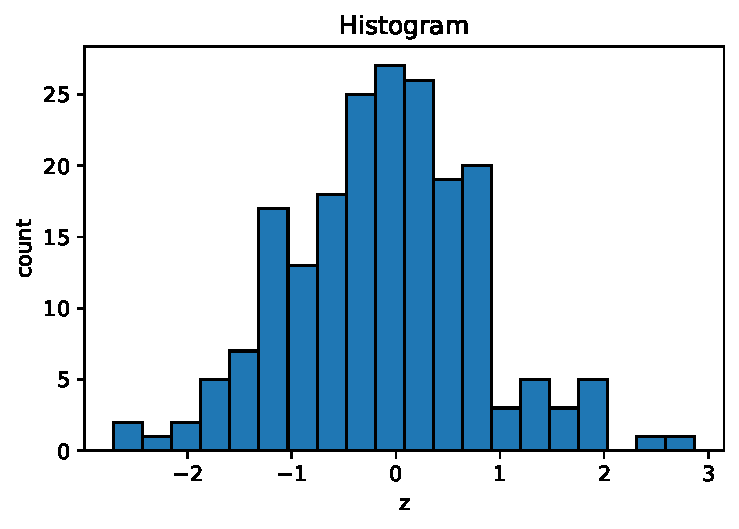
\includegraphics[keepaspectratio]{contents/app/python_files/figure-pdf/cell-50-output-1.pdf}}

\section{Common Errors}\label{common-errors}

\subsection{\texorpdfstring{One-Dimensional
\texttt{X}}{One-Dimensional X}}\label{one-dimensional-x}

The most common error is passing a one-dimensional predictor array to
\texttt{sklearn}.

{\def\LTcaptype{none} % do not increment counter
\begin{longtable}[]{@{}
  >{\raggedright\arraybackslash}p{(\linewidth - 2\tabcolsep) * \real{0.5000}}
  >{\raggedright\arraybackslash}p{(\linewidth - 2\tabcolsep) * \real{0.5000}}@{}}
\toprule\noalign{}
\begin{minipage}[b]{\linewidth}\raggedright
Bad
\end{minipage} & \begin{minipage}[b]{\linewidth}\raggedright
Good
\end{minipage} \\
\midrule\noalign{}
\endhead
\bottomrule\noalign{}
\endlastfoot
\texttt{x\ =\ np.array({[}1,\ 2,\ 3,\ 4{]})}\texttt{model.fit(x,\ y)} &
\texttt{X\ =\ x.reshape(-1,\ 1)}\texttt{model.fit(X,\ y)} \\
\end{longtable}
}

\subsection{Class Name versus Model
Object}\label{class-name-versus-model-object}

Another common mistake is confusing an \texttt{sklearn} class with an
object created from that class.

For example, \texttt{DecisionTreeClassifier} is the class itself.

{\def\LTcaptype{none} % do not increment counter
\begin{longtable}[]{@{}
  >{\raggedright\arraybackslash}p{(\linewidth - 2\tabcolsep) * \real{0.5000}}
  >{\raggedright\arraybackslash}p{(\linewidth - 2\tabcolsep) * \real{0.5000}}@{}}
\toprule\noalign{}
\begin{minipage}[b]{\linewidth}\raggedright
Wrong
\end{minipage} & \begin{minipage}[b]{\linewidth}\raggedright
Right
\end{minipage} \\
\midrule\noalign{}
\endhead
\bottomrule\noalign{}
\endlastfoot
\texttt{model\ =\ DecisionTreeClassifier}\texttt{model.fit(X\_train,\ y\_train)}
&
\texttt{model\ =\ DecisionTreeClassifier()}\texttt{model.fit(X\_train,\ y\_train)} \\
\end{longtable}
}

\subsection{Mixing Lists and Arrays}\label{mixing-lists-and-arrays}

Use arrays for elementwise numerical operations.

\begin{Shaded}
\begin{Highlighting}[]
\NormalTok{[}\DecValTok{1}\NormalTok{, }\DecValTok{2}\NormalTok{, }\DecValTok{3}\NormalTok{] }\OperatorTok{*} \DecValTok{2}
\end{Highlighting}
\end{Shaded}

\begin{verbatim}
[1, 2, 3, 1, 2, 3]
\end{verbatim}

Plain lists do not always behave like numerical vectors.

\begin{Shaded}
\begin{Highlighting}[]
\ImportTok{import}\NormalTok{ numpy }\ImportTok{as}\NormalTok{ np}

\NormalTok{np.array([}\DecValTok{1}\NormalTok{, }\DecValTok{2}\NormalTok{, }\DecValTok{3}\NormalTok{]) }\OperatorTok{*} \DecValTok{2}
\end{Highlighting}
\end{Shaded}

\begin{verbatim}
array([2, 4, 6])
\end{verbatim}

\chapter{Some Python concepts}\label{some-python-concepts}

\section{Language}\label{language}

Python is a programming language. In other words, it is a collection of
syntaxes.

\section{Interpreters}\label{interpreters}

Python needs to be interpreted into codes that computers can understand.
Therefore there should be some programs that translate Python scripts.
These programs are called \emph{interpreters}.

\texttt{CPython} is the reference implementation of Python and the
implementation most people use. It is written mainly in C and Python.
New Python language features are normally developed and tested first in
CPython.

Other implementations include
\href{https://www.pypy.org/}{\texttt{PyPy}},
\href{https://www.jython.org/}{\texttt{Jython}} and
\href{https://ironpython.net/}{\texttt{IronPython}}. They are useful in
specific contexts, but they do not always support the same Python
versions or the same package ecosystem as CPython. For example, PyPy
focuses on speed through a JIT compiler, Jython integrates with the JVM
but its current stable release is Python 2.7-based, and IronPython
integrates with .NET but lags behind modern CPython versions.

Since \texttt{CPython} is the most widely used and best-supported
implementation, it is the best choice, at least for beginners. And
actually, if you have no idea about this topic, but you use Python, it
is highly possible that you are using \texttt{CPython}.

\begin{tcolorbox}[enhanced jigsaw, arc=.35mm, bottomrule=.15mm, bottomtitle=1mm, breakable, colback=white, colbacktitle=quarto-callout-note-color!10!white, colframe=quarto-callout-note-color-frame, coltitle=black, left=2mm, leftrule=.75mm, opacityback=0, opacitybacktitle=0.6, rightrule=.15mm, title=\textcolor{quarto-callout-note-color}{\faInfo}\hspace{0.5em}{Note}, titlerule=0mm, toprule=.15mm, toptitle=1mm]

We mentioned ``interpreter'' here. There are mainly two types of
implimentations of programming langauges: interpreters and compilers.
There are also some additional types like just-in-time compilers which
can be treated as combinations of the two.

Python is often described as an \emph{interpreted} language, but
\texttt{CPython} first compiles source code to bytecode and then
executes that bytecode in the Python virtual machine. For beginners, the
practical point is that Python supports an interactive workflow and does
not require a separate manual compile step.

\end{tcolorbox}

\section{REPL}\label{repl}

There are two ways to use Python interpreter. One way is to execute a
Python script stored in a file. The second way is called \emph{the
intereactive shell}, that Python interpreter read the input from user
directly, and print the result immediately. The model is like code
example: prompt the user for some code, and when they've entered it,
execute it in the same process. This model is often called a
\href{https://en.wikipedia.org/wiki/Read\%E2\%80\%93eval\%E2\%80\%93print_loop}{REPL},
or \emph{Read-Eval-Print-Loop}.

\emph{Shell}, \emph{terminal}, \emph{console} have different meanings in
their original contexts. However, nowadays, especially when talking
about Python intereactive shell, these terminologies are used
interchangeably. They are referred to the frontend of the system. In
other words, the main task for the Python intereactive shell is to
handle the user inputs and communicate with the backend, which is also
called a \emph{kernel}. We won't distinguish the real differences
between these terminologies. The kernel will be discussed in the next
section.

The standard Python REPL can usually be started with \texttt{python} or
\texttt{python3}. On Windows, \texttt{py} may also be available. To
quit, use \texttt{quit()}, \texttt{exit()}, \texttt{Ctrl+D} on
macOS/Linux, or \texttt{Ctrl+Z} then \texttt{Enter} on Windows.

\begin{tcolorbox}[enhanced jigsaw, arc=.35mm, bottomrule=.15mm, bottomtitle=1mm, breakable, colback=white, colbacktitle=quarto-callout-note-color!10!white, colframe=quarto-callout-note-color-frame, coltitle=black, left=2mm, leftrule=.75mm, opacityback=0, opacitybacktitle=0.6, rightrule=.15mm, title=\textcolor{quarto-callout-note-color}{\faInfo}\hspace{0.5em}{Note}, titlerule=0mm, toprule=.15mm, toptitle=1mm]

In the REPL model, the backend (evaluation) is basically handled by the
Python interpreter. The frontend is dealing with the user interface.
Some typically tasks include the \emph{primary/secondary prompt} and
multi-line commands. The original REPL is very limited.

\end{tcolorbox}

\section{\texorpdfstring{\texttt{IPython}}{IPython}}\label{ipython}

\texttt{IPython} was initially designed as an Enhanced interactive
Python shell. However after many year's development, the whole
\texttt{IPython} project becomes too big to maintain as one single
project. Therefore it is now split into many smaller projects. The two
most popular projects are \texttt{IPython} and \texttt{Jupyter}. This is
called \href{https://blog.jupyter.org/the-big-split-9d7b88a031a7}{the
Big Split}.

The current
\href{https://ipython.readthedocs.io/en/stable/overview.html}{\texttt{IPython}}
play two fundamental roles:

\begin{itemize}
\tightlist
\item
  Terminal \texttt{IPython} as the familiar REPL;
\item
  The \texttt{IPython} kernel (which is defined below) that provides
  computation and communication with the frontend interfaces, like the
  notebook.
\end{itemize}

The core idea in the design of \texttt{IPython} is to abstract and
extend the notion of a traditional REPL environment by decoupling the
evaluation into its own process. We call this process a \emph{kernel}:
it receives execution instructions from clients and communicates the
results back to them.

This decoupling allows us to have several clients connected to the same
kernel, and even allows clients and kernels to live on different
machines. This two-process model is now used by most of the
\texttt{Jupyter} project.

You can launch the \texttt{IPython} shell on the command line with the
\texttt{ipython} command (which similar to \texttt{python} case requires
\texttt{PATH} configuration), and quit the shell with
\texttt{exit}/\texttt{exit()}/\texttt{quit}/\texttt{quit()} commands.

The reference Python kernel provided by \texttt{IPython} is called
\texttt{ipykernel}. With \texttt{ipykernel} you may create and maintain
multiple kernels.

\section{\texorpdfstring{\texttt{Jupyter}}{Jupyter}}\label{jupyter}

\href{https://docs.jupyter.org/en/latest/projects/architecture/content-architecture.html}{\texttt{Jupyter}}
is an ecosystem for interactive computing. It originated from the
IPython Notebook project and later evolved into a language-independent
platform supporting many programming languages. The name
\textbf{Jupyter} is inspired by \textbf{Julia}, \textbf{Python}, and
\textbf{R}, the three languages that were central to many early data
science workflows.

Today, Jupyter includes several user interfaces, such as JupyterLab,
Jupyter Notebook, Jupyter Console, and QtConsole. In this course,
however, the important idea is not a particular interface, but the
relationship among a notebook frontend, a kernel, and the notebook file
stored on disk.

A Jupyter notebook is saved as a file with extension \texttt{.ipynb}.
Internally, the file uses a structured \texttt{JSON} format that stores:

\begin{itemize}
\tightlist
\item
  code cells;
\item
  Markdown cells;
\item
  outputs;
\item
  notebook metadata.
\end{itemize}

When you run code in a notebook, the frontend sends the code to a
kernel, which executes the code and returns the results. In a Python
notebook, a kernel can be viewed as a Python process running in the
background. It executes code, stores variables, and communicates with
the notebook interface.

Different programming languages can be supported by different kernels.
For example:

\begin{itemize}
\tightlist
\item
  \texttt{ipykernel} for Python;
\item
  \texttt{IRkernel} for R;
\item
  \texttt{IJulia} for Julia.
\end{itemize}

\begin{tcolorbox}[enhanced jigsaw, arc=.35mm, bottomrule=.15mm, bottomtitle=1mm, breakable, colback=white, colbacktitle=quarto-callout-note-color!10!white, colframe=quarto-callout-note-color-frame, coltitle=black, left=2mm, leftrule=.75mm, opacityback=0, opacitybacktitle=0.6, rightrule=.15mm, title=\textcolor{quarto-callout-note-color}{\faInfo}\hspace{0.5em}{Kernel}, titlerule=0mm, toprule=.15mm, toptitle=1mm]

A kernel is associated with a particular Python environment, but it is
not the environment itself. For example, multiple kernels may use the
same Python environment while maintaining completely separate variables
and memory. Conversely, multiple notebook windows may connect to the
same kernel and therefore share the same variables and computational
state.

For this course, you can think of the notebook as the user interface,
the kernel as the Python process that runs your code, and the
\texttt{.ipynb} file as the notebook document saved on disk.

\end{tcolorbox}

\subsection{Multi-kernels setup}\label{multi-kernels-setup}

This section is mainly following the
\href{https://ipython.readthedocs.io/en/stable/install/kernel_install.html}{official
document}.

To install one \texttt{IPython} kernel, you may install
\texttt{ipykernel} in the environment. If you want to have multiple
\texttt{IPython} kernels for different venvs, you will need to specify
unique names for the kernelspecs.

\begin{enumerate}
\def\labelenumi{\arabic{enumi}.}
\tightlist
\item
  Activate the environment you want.
\item
  Install the kernel in the environment.
\end{enumerate}

\begin{Shaded}
\begin{Highlighting}[]
\ExtensionTok{uv}\NormalTok{ add ipykernel}
\ExtensionTok{uv}\NormalTok{ run python }\AttributeTok{{-}m}\NormalTok{ ipykernel install }\AttributeTok{{-}{-}user} \AttributeTok{{-}{-}name}\NormalTok{ myenv }\AttributeTok{{-}{-}display{-}name} \StringTok{"Python (myenv)"}
\end{Highlighting}
\end{Shaded}

\texttt{-\/-user} means that the kernel is installed in the user's
folder instead of a system folder, and it can be removed. The
\texttt{-\/-name} value (in this case it is \texttt{myenv}) is used by
Jupyter internally. These commands will overwrite any existing kernel
with the same name. \texttt{-\/-display-name} is what you see in the
notebook menus.

\begin{enumerate}
\def\labelenumi{\arabic{enumi}.}
\setcounter{enumi}{2}
\tightlist
\item
  You could use the command to find all kernels installed in your
  system.
\end{enumerate}

\begin{Shaded}
\begin{Highlighting}[]
\ExtensionTok{uv}\NormalTok{ run jupyter kernelspec list}
\end{Highlighting}
\end{Shaded}

Available kernels are shown, as well as the path to the kernel
configuration file \texttt{kernel.json}. The most important
configuration is the path to the Python interpreter executatable file.

\begin{codelisting}

\caption{\texttt{kernel.json}}

\begin{Shaded}
\begin{Highlighting}[]
\FunctionTok{\{}
 \DataTypeTok{"argv"}\FunctionTok{:} \OtherTok{[}
  \StringTok{"C:}\CharTok{\textbackslash{}\textbackslash{}}\StringTok{Users}\CharTok{\textbackslash{}\textbackslash{}}\StringTok{WDAGUtilityAccount}\CharTok{\textbackslash{}\textbackslash{}}\StringTok{Project}\CharTok{\textbackslash{}\textbackslash{}}\StringTok{.venv}\CharTok{\textbackslash{}\textbackslash{}}\StringTok{Scripts}\CharTok{\textbackslash{}\textbackslash{}}\StringTok{python.exe"}\OtherTok{,}
  \StringTok{"{-}Xfrozen\_modules=off"}\OtherTok{,}
  \StringTok{"{-}m"}\OtherTok{,}
  \StringTok{"ipykernel\_launcher"}\OtherTok{,}
  \StringTok{"{-}f"}\OtherTok{,}
  \StringTok{"\{connection\_file\}"}
 \OtherTok{]}\FunctionTok{,}
 \DataTypeTok{"display\_name"}\FunctionTok{:} \StringTok{"(myenv)"}\FunctionTok{,}
 \DataTypeTok{"language"}\FunctionTok{:} \StringTok{"python"}\FunctionTok{,}
 \DataTypeTok{"metadata"}\FunctionTok{:} \FunctionTok{\{}
  \DataTypeTok{"debugger"}\FunctionTok{:} \KeywordTok{true}
 \FunctionTok{\},}
 \DataTypeTok{"kernel\_protocol\_version"}\FunctionTok{:} \StringTok{"5.5"}
\FunctionTok{\}}
\end{Highlighting}
\end{Shaded}

\end{codelisting}

Notice that the path in \texttt{argv} points to the Python interpreter
used by this kernel. Different kernels may point to different Python
environments, or multiple kernels may point to the same environment.

\chapter{Data Processing and EDA}\label{data-processing-and-eda}

This note uses the synthetic \href{minidataset.csv}{dataset
\texttt{minidataset.csv}} to demonstrate essential data-processing and
EDA operations. The dataset contains repeated measurements from several
individuals, each with up to three visits. Each row represents one visit
for one individual.

This note provides brief examples rather than comprehensive instructions
for each command. If you choose to use a command in your project,
consult its documentation and make sure you apply it appropriately to
your data and analysis.

\section{Load and inspect the data}\label{load-and-inspect-the-data}

\begin{Shaded}
\begin{Highlighting}[]
\ImportTok{import}\NormalTok{ pandas }\ImportTok{as}\NormalTok{ pd}

\NormalTok{df }\OperatorTok{=}\NormalTok{ pd.read\_csv(}\StringTok{"minidataset.csv"}\NormalTok{)}
\NormalTok{df.head()}
\end{Highlighting}
\end{Shaded}

{\def\LTcaptype{none} % do not increment counter
\begin{longtable}[]{@{}lllllllllllll@{}}
\toprule\noalign{}
& id & visit & time & num\_1 & cat\_1 & num\_2 & num\_3 & num\_4 &
cat\_2 & num\_5 & cat\_3 & target \\
\midrule\noalign{}
\endhead
\bottomrule\noalign{}
\endlastfoot
0 & 1001 & 1 & 0 & 45 & F & 118 & 23.8 & 188.0 & 0 & 0 & 0 & 0 \\
1 & 1001 & 2 & 2130 & 51 & F & 122 & 24.1 & 194.0 & 0 & 0 & 0 & 0 \\
2 & 1001 & 3 & 4280 & 57 & F & 126 & 24.5 & 201.0 & 0 & 0 & 0 & 0 \\
3 & 1002 & 1 & 0 & 52 & M & 132 & 27.4 & 221.0 & 1 & 15 & 0 & 0 \\
4 & 1002 & 2 & 2085 & 58 & M & 138 & 28.0 & 229.0 & 1 & 12 & 0 & 0 \\
\end{longtable}
}

The variable \texttt{id} identifies the individual, \texttt{visit}
records the visit number, and \texttt{time} records the number of days
since baseline.

\begin{Shaded}
\begin{Highlighting}[]
\BuiltInTok{print}\NormalTok{(}\SpecialStringTok{f"Rows, Columns: }\SpecialCharTok{\{}\NormalTok{df}\SpecialCharTok{.}\NormalTok{shape}\SpecialCharTok{\}}\SpecialStringTok{"}\NormalTok{)}
\BuiltInTok{print}\NormalTok{(}\SpecialStringTok{f"Individuals: }\SpecialCharTok{\{}\NormalTok{df[}\StringTok{\textquotesingle{}id\textquotesingle{}}\NormalTok{]}\SpecialCharTok{.}\NormalTok{nunique()}\SpecialCharTok{\}}\SpecialStringTok{"}\NormalTok{)}
\end{Highlighting}
\end{Shaded}

\begin{verbatim}
Rows, Columns: (32, 12)
Individuals: 12
\end{verbatim}

Count the number of visits recorded for each individual:

\begin{Shaded}
\begin{Highlighting}[]
\NormalTok{visits\_per\_id }\OperatorTok{=}\NormalTok{ df.groupby(}\StringTok{"id"}\NormalTok{).size()}
\NormalTok{visits\_per\_id.head()}
\end{Highlighting}
\end{Shaded}

\begin{verbatim}
id
1001    3
1002    3
1003    2
1004    3
1005    3
dtype: int64
\end{verbatim}

Each value is the number of rows, or visits, available for one
\texttt{id}.

\section{Merge visits into one row per
individual}\label{merge-visits-into-one-row-per-individual}

Use \texttt{pivot()} to place different visits from the same \texttt{id}
on one row. To keep the example concise, we select only \texttt{num\_1}
and \texttt{num\_2}.

\begin{Shaded}
\begin{Highlighting}[]
\NormalTok{wide }\OperatorTok{=}\NormalTok{ df.pivot(index}\OperatorTok{=}\StringTok{"id"}\NormalTok{, columns}\OperatorTok{=}\StringTok{"visit"}\NormalTok{, values}\OperatorTok{=}\NormalTok{[}\StringTok{"num\_1"}\NormalTok{, }\StringTok{"num\_2"}\NormalTok{])}
\NormalTok{wide.head()}
\end{Highlighting}
\end{Shaded}

{\def\LTcaptype{none} % do not increment counter
\begin{longtable}[]{@{}lllllll@{}}
\toprule\noalign{}
& \multicolumn{3}{l}{%
num\_1} & \multicolumn{3}{l@{}}{%
num\_2} \\
visit & 1 & 2 & 3 & 1 & 2 & 3 \\
id & & & & & & \\
\midrule\noalign{}
\endhead
\bottomrule\noalign{}
\endlastfoot
1001 & 45.0 & 51.0 & 57.0 & 118.0 & 122.0 & 126.0 \\
1002 & 52.0 & 58.0 & 64.0 & 132.0 & 138.0 & 146.0 \\
1003 & 39.0 & 45.0 & NaN & 110.0 & 112.0 & NaN \\
1004 & 60.0 & 66.0 & 72.0 & 148.0 & 156.0 & 164.0 \\
1005 & 48.0 & 54.0 & 60.0 & 124.0 & 128.0 & 134.0 \\
\end{longtable}
}

Reset the index and assign simple column names to make the resulting
DataFrame easier to use:

\begin{Shaded}
\begin{Highlighting}[]
\NormalTok{wide.columns }\OperatorTok{=}\NormalTok{ [}\SpecialStringTok{f"}\SpecialCharTok{\{}\NormalTok{variable}\SpecialCharTok{\}}\SpecialStringTok{\_v}\SpecialCharTok{\{}\NormalTok{visit}\SpecialCharTok{\}}\SpecialStringTok{"} \ControlFlowTok{for}\NormalTok{ variable, visit }\KeywordTok{in}\NormalTok{ wide.columns]}
\NormalTok{wide }\OperatorTok{=}\NormalTok{ wide.reset\_index()}
\NormalTok{wide.head()}
\end{Highlighting}
\end{Shaded}

{\def\LTcaptype{none} % do not increment counter
\begin{longtable}[]{@{}llllllll@{}}
\toprule\noalign{}
& id & num\_1\_v1 & num\_1\_v2 & num\_1\_v3 & num\_2\_v1 & num\_2\_v2 &
num\_2\_v3 \\
\midrule\noalign{}
\endhead
\bottomrule\noalign{}
\endlastfoot
0 & 1001 & 45.0 & 51.0 & 57.0 & 118.0 & 122.0 & 126.0 \\
1 & 1002 & 52.0 & 58.0 & 64.0 & 132.0 & 138.0 & 146.0 \\
2 & 1003 & 39.0 & 45.0 & NaN & 110.0 & 112.0 & NaN \\
3 & 1004 & 60.0 & 66.0 & 72.0 & 148.0 & 156.0 & 164.0 \\
4 & 1005 & 48.0 & 54.0 & 60.0 & 124.0 & 128.0 & 134.0 \\
\end{longtable}
}

The result contains one row per individual.

\section{Avoid data leakage}\label{avoid-data-leakage}

To keep all visits from the same individual together, there are at least
two different methods:

\begin{enumerate}
\def\labelenumi{\arabic{enumi}.}
\tightlist
\item
  Reshape the data so that all visits from the same individual appear in
  one row (using the method mentioned above), and then split by rows.
\item
  Split the unique IDs and then select their rows.
\end{enumerate}

\begin{Shaded}
\begin{Highlighting}[]
\ImportTok{from}\NormalTok{ sklearn.model\_selection }\ImportTok{import}\NormalTok{ train\_test\_split}

\NormalTok{ids }\OperatorTok{=}\NormalTok{ df[}\StringTok{"id"}\NormalTok{].drop\_duplicates()}

\NormalTok{train\_ids, remaining\_ids }\OperatorTok{=}\NormalTok{ train\_test\_split(ids, test\_size}\OperatorTok{=}\FloatTok{0.40}\NormalTok{, random\_state}\OperatorTok{=}\DecValTok{1}\NormalTok{)}
\NormalTok{val\_ids, test\_ids }\OperatorTok{=}\NormalTok{ train\_test\_split(remaining\_ids, test\_size}\OperatorTok{=}\FloatTok{0.50}\NormalTok{, random\_state}\OperatorTok{=}\DecValTok{1}\NormalTok{)}

\NormalTok{train\_df }\OperatorTok{=}\NormalTok{ df.loc[df[}\StringTok{"id"}\NormalTok{].isin(train\_ids)].copy()}
\NormalTok{val\_df }\OperatorTok{=}\NormalTok{ df.loc[df[}\StringTok{"id"}\NormalTok{].isin(val\_ids)].copy()}
\NormalTok{test\_df }\OperatorTok{=}\NormalTok{ df.loc[df[}\StringTok{"id"}\NormalTok{].isin(test\_ids)].copy()}
\end{Highlighting}
\end{Shaded}

\section{Summarize and handle missing
values}\label{summarize-and-handle-missing-values}

Use \texttt{info()} to inspect the data types and non-null count for
each column. A non-null count below the total number of rows indicates
missing values:

\begin{Shaded}
\begin{Highlighting}[]
\NormalTok{df.info()}
\end{Highlighting}
\end{Shaded}

\begin{verbatim}
<class 'pandas.DataFrame'>
RangeIndex: 32 entries, 0 to 31
Data columns (total 12 columns):
 #   Column  Non-Null Count  Dtype  
---  ------  --------------  -----  
 0   id      32 non-null     int64  
 1   visit   32 non-null     int64  
 2   time    32 non-null     int64  
 3   num_1   32 non-null     int64  
 4   cat_1   32 non-null     str    
 5   num_2   32 non-null     int64  
 6   num_3   31 non-null     float64
 7   num_4   31 non-null     float64
 8   cat_2   32 non-null     int64  
 9   num_5   32 non-null     int64  
 10  cat_3   32 non-null     int64  
 11  target  32 non-null     int64  
dtypes: float64(2), int64(9), str(1)
memory usage: 3.1 KB
\end{verbatim}

For missing values, we could either drop them

\begin{Shaded}
\begin{Highlighting}[]
\NormalTok{df\_dropped }\OperatorTok{=}\NormalTok{ df.dropna()}
\end{Highlighting}
\end{Shaded}

\begin{tcolorbox}[enhanced jigsaw, arc=.35mm, bottomrule=.15mm, bottomtitle=1mm, breakable, colback=white, colbacktitle=quarto-callout-caution-color!10!white, colframe=quarto-callout-caution-color-frame, coltitle=black, left=2mm, leftrule=.75mm, opacityback=0, opacitybacktitle=0.6, rightrule=.15mm, title=\textcolor{quarto-callout-caution-color}{\faFire}\hspace{0.5em}{Caution}, titlerule=0mm, toprule=.15mm, toptitle=1mm]

Be careful: \texttt{dropna()} removes every row that contains at least
one missing value.

\end{tcolorbox}

Alternatively, we could use \texttt{fillna()} to replace missing values
with a specified value, such as \(0\):

\begin{Shaded}
\begin{Highlighting}[]
\NormalTok{df\_filled\_0 }\OperatorTok{=}\NormalTok{ df.fillna(}\DecValTok{0}\NormalTok{)}
\end{Highlighting}
\end{Shaded}

or we could use \texttt{fillna()} to replace missing values with the
column mean:

\begin{Shaded}
\begin{Highlighting}[]
\NormalTok{df\_filled }\OperatorTok{=}\NormalTok{ df.copy()}
\NormalTok{df\_filled[}\StringTok{"num\_3"}\NormalTok{] }\OperatorTok{=}\NormalTok{ df\_filled[}\StringTok{"num\_3"}\NormalTok{].fillna(df\_filled[}\StringTok{"num\_3"}\NormalTok{].mean())}
\end{Highlighting}
\end{Shaded}

Missing values can also be filled with the mean of each group. This
example uses the mean within each \texttt{cat\_1} group:

\begin{Shaded}
\begin{Highlighting}[]
\NormalTok{df\_group\_filled }\OperatorTok{=}\NormalTok{ df.copy()}
\NormalTok{group\_mean }\OperatorTok{=}\NormalTok{ df.groupby(}\StringTok{"cat\_1"}\NormalTok{)[}\StringTok{"num\_3"}\NormalTok{].transform(}\StringTok{"mean"}\NormalTok{)}
\NormalTok{df\_group\_filled[}\StringTok{"num\_3"}\NormalTok{] }\OperatorTok{=}\NormalTok{ df\_group\_filled[}\StringTok{"num\_3"}\NormalTok{].fillna(group\_mean)}
\end{Highlighting}
\end{Shaded}

\begin{tcolorbox}[enhanced jigsaw, arc=.35mm, bottomrule=.15mm, bottomtitle=1mm, breakable, colback=white, colbacktitle=quarto-callout-note-color!10!white, colframe=quarto-callout-note-color-frame, coltitle=black, left=2mm, leftrule=.75mm, opacityback=0, opacitybacktitle=0.6, rightrule=.15mm, title=\textcolor{quarto-callout-note-color}{\faInfo}\hspace{0.5em}{Imputer}, titlerule=0mm, toprule=.15mm, toptitle=1mm]

The examples above show simple approaches to missing-value imputation. A
more complete, cross-validation-safe approach typically combines a
\texttt{sklearn} imputer with \texttt{ColumnTransformer} and
\texttt{Pipeline}, so that imputation is fitted separately within each
training fold and applied consistently to other data. The details of
this approach are beyond the scope of this note.

\end{tcolorbox}

\section{Construct features}\label{construct-features}

Sort by individual and time before calculating within-person
differences:

\begin{Shaded}
\begin{Highlighting}[]
\NormalTok{df\_sort }\OperatorTok{=}\NormalTok{ df.sort\_values([}\StringTok{"id"}\NormalTok{, }\StringTok{"time"}\NormalTok{]).copy()}

\NormalTok{df\_sort[}\StringTok{"time\_change"}\NormalTok{] }\OperatorTok{=}\NormalTok{ df\_sort.groupby(}\StringTok{"id"}\NormalTok{)[}\StringTok{"time"}\NormalTok{].diff()}
\NormalTok{df\_sort[}\StringTok{"num\_2\_change"}\NormalTok{] }\OperatorTok{=}\NormalTok{ df\_sort.groupby(}\StringTok{"id"}\NormalTok{)[}\StringTok{"num\_2"}\NormalTok{].diff()}
\NormalTok{df\_sort[}\StringTok{"num\_2\_change\_per\_day"}\NormalTok{] }\OperatorTok{=}\NormalTok{ df\_sort[}\StringTok{"num\_2\_change"}\NormalTok{] }\OperatorTok{/}\NormalTok{ (df\_sort[}\StringTok{"time\_change"}\NormalTok{])}

\NormalTok{df\_sort.head()}
\end{Highlighting}
\end{Shaded}

{\def\LTcaptype{none} % do not increment counter
\begin{longtable}[]{@{}llllllllllllllll@{}}
\toprule\noalign{}
& id & visit & time & num\_1 & cat\_1 & num\_2 & num\_3 & num\_4 &
cat\_2 & num\_5 & cat\_3 & target & time\_change & num\_2\_change &
num\_2\_change\_per\_day \\
\midrule\noalign{}
\endhead
\bottomrule\noalign{}
\endlastfoot
0 & 1001 & 1 & 0 & 45 & F & 118 & 23.8 & 188.0 & 0 & 0 & 0 & 0 & NaN &
NaN & NaN \\
1 & 1001 & 2 & 2130 & 51 & F & 122 & 24.1 & 194.0 & 0 & 0 & 0 & 0 &
2130.0 & 4.0 & 0.001878 \\
2 & 1001 & 3 & 4280 & 57 & F & 126 & 24.5 & 201.0 & 0 & 0 & 0 & 0 &
2150.0 & 4.0 & 0.001860 \\
3 & 1002 & 1 & 0 & 52 & M & 132 & 27.4 & 221.0 & 1 & 15 & 0 & 0 & NaN &
NaN & NaN \\
4 & 1002 & 2 & 2085 & 58 & M & 138 & 28.0 & 229.0 & 1 & 12 & 0 & 0 &
2085.0 & 6.0 & 0.002878 \\
\end{longtable}
}

Only information observed before the prediction time may be used to
construct predictors.

\section{Combine numerical values into
groups}\label{combine-numerical-values-into-groups}

Use \texttt{pd.cut()} when predefined, ordered intervals have a
meaningful interpretation:

\begin{Shaded}
\begin{Highlighting}[]
\NormalTok{df[}\StringTok{"num\_1\_group"}\NormalTok{] }\OperatorTok{=}\NormalTok{ pd.cut(}
\NormalTok{    df[}\StringTok{"num\_1"}\NormalTok{],}
\NormalTok{    bins}\OperatorTok{=}\NormalTok{[}\BuiltInTok{float}\NormalTok{(}\StringTok{"{-}inf"}\NormalTok{), }\DecValTok{45}\NormalTok{, }\DecValTok{55}\NormalTok{, }\DecValTok{65}\NormalTok{, }\BuiltInTok{float}\NormalTok{(}\StringTok{"inf"}\NormalTok{)],}
\NormalTok{    labels}\OperatorTok{=}\NormalTok{[}\StringTok{"below\_45"}\NormalTok{, }\StringTok{"45{-}54"}\NormalTok{, }\StringTok{"55{-}64"}\NormalTok{, }\StringTok{"65\_or\_above"}\NormalTok{],}
\NormalTok{    right}\OperatorTok{=}\VariableTok{False}\NormalTok{,}
\NormalTok{    ordered}\OperatorTok{=}\VariableTok{True}\NormalTok{,}
\NormalTok{)}

\NormalTok{df[}\StringTok{"num\_1\_group"}\NormalTok{].head(}\DecValTok{9}\NormalTok{)}
\end{Highlighting}
\end{Shaded}

\begin{verbatim}
0       45-54
1       45-54
2       55-64
3       45-54
4       55-64
5       55-64
6    below_45
7       45-54
8       55-64
Name: num_1_group, dtype: category
Categories (4, str): ['below_45' < '45-54' < '55-64' < '65_or_above']
\end{verbatim}

Choose cut points using subject-matter knowledge or the training data
only, not the validation or test set.

\section{Perform concise EDA}\label{perform-concise-eda}

\subsection{Summary statistics}\label{summary-statistics}

\begin{Shaded}
\begin{Highlighting}[]
\NormalTok{df.describe()}
\end{Highlighting}
\end{Shaded}

{\def\LTcaptype{none} % do not increment counter
\begin{longtable}[]{@{}llllllllllll@{}}
\toprule\noalign{}
& id & visit & time & num\_1 & num\_2 & num\_3 & num\_4 & cat\_2 &
num\_5 & cat\_3 & target \\
\midrule\noalign{}
\endhead
\bottomrule\noalign{}
\endlastfoot
count & 32.000000 & 32.000000 & 32.000000 & 32.000000 & 32.000000 &
31.000000 & 31.000000 & 32.000000 & 32.00000 & 32.000000 & 32.000000 \\
mean & 1006.156250 & 1.906250 & 1917.656250 & 55.468750 & 135.125000 &
27.403226 & 219.967742 & 0.437500 & 5.96875 & 0.250000 & 0.218750 \\
std & 3.322546 & 0.817525 & 1733.112985 & 8.481419 & 15.009137 &
2.892114 & 24.895092 & 0.504016 & 7.70205 & 0.439941 & 0.420013 \\
min & 1001.000000 & 1.000000 & 0.000000 & 39.000000 & 110.000000 &
21.900000 & 174.000000 & 0.000000 & 0.00000 & 0.000000 & 0.000000 \\
25\% & 1003.750000 & 1.000000 & 0.000000 & 49.500000 & 123.500000 &
25.150000 & 200.000000 & 0.000000 & 0.00000 & 0.000000 & 0.000000 \\
50\% & 1006.000000 & 2.000000 & 2077.500000 & 56.500000 & 135.000000 &
27.900000 & 221.000000 & 0.000000 & 0.00000 & 0.000000 & 0.000000 \\
75\% & 1009.000000 & 3.000000 & 4128.750000 & 61.250000 & 146.500000 &
29.800000 & 240.500000 & 1.000000 & 10.50000 & 0.250000 & 0.000000 \\
max & 1012.000000 & 3.000000 & 4375.000000 & 72.000000 & 164.000000 &
32.000000 & 260.000000 & 1.000000 & 25.00000 & 1.000000 & 1.000000 \\
\end{longtable}
}

\subsection{Outcome class balance}\label{outcome-class-balance}

\begin{Shaded}
\begin{Highlighting}[]
\NormalTok{df[}\StringTok{"target"}\NormalTok{].value\_counts(normalize}\OperatorTok{=}\VariableTok{True}\NormalTok{, dropna}\OperatorTok{=}\VariableTok{False}\NormalTok{)}
\end{Highlighting}
\end{Shaded}

\begin{verbatim}
target
0    0.78125
1    0.21875
Name: proportion, dtype: float64
\end{verbatim}

\subsection{Comparison between outcome
groups}\label{comparison-between-outcome-groups}

\begin{Shaded}
\begin{Highlighting}[]
\NormalTok{important\_num }\OperatorTok{=}\NormalTok{ [}\StringTok{"num\_1"}\NormalTok{, }\StringTok{"num\_2"}\NormalTok{, }\StringTok{"num\_3"}\NormalTok{, }\StringTok{"num\_4"}\NormalTok{]}
\NormalTok{df.groupby(}\StringTok{"target"}\NormalTok{, dropna}\OperatorTok{=}\VariableTok{False}\NormalTok{)[important\_num].mean().T}
\end{Highlighting}
\end{Shaded}

{\def\LTcaptype{none} % do not increment counter
\begin{longtable}[]{@{}lll@{}}
\toprule\noalign{}
target & 0 & 1 \\
\midrule\noalign{}
\endhead
\bottomrule\noalign{}
\endlastfoot
num\_1 & 52.440000 & 66.285714 \\
num\_2 & 129.760000 & 154.285714 \\
num\_3 & 26.583333 & 30.214286 \\
num\_4 & 211.625000 & 248.571429 \\
\end{longtable}
}

\subsection{Correlation heatmap}\label{correlation-heatmap}

\begin{Shaded}
\begin{Highlighting}[]
\ImportTok{import}\NormalTok{ seaborn }\ImportTok{as}\NormalTok{ sns}
\ImportTok{import}\NormalTok{ matplotlib.pyplot }\ImportTok{as}\NormalTok{ plt}

\NormalTok{sns.heatmap(df[important\_num].corr(), annot}\OperatorTok{=}\VariableTok{True}\NormalTok{, cmap}\OperatorTok{=}\StringTok{"coolwarm"}\NormalTok{, vmin}\OperatorTok{={-}}\DecValTok{1}\NormalTok{, vmax}\OperatorTok{=}\DecValTok{1}\NormalTok{)}
\NormalTok{plt.title(}\StringTok{"Correlations among Important Variables"}\NormalTok{)}\OperatorTok{;}
\end{Highlighting}
\end{Shaded}

\pandocbounded{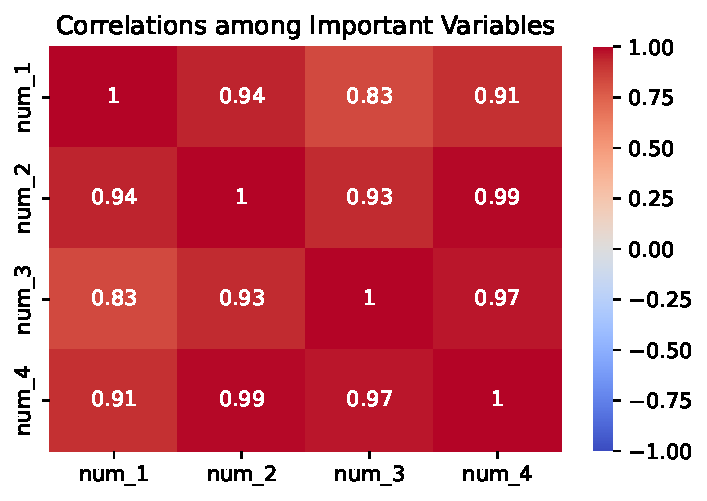
\includegraphics[keepaspectratio]{contents/app/preprocessing-eda_files/figure-pdf/cell-18-output-1.pdf}}

Choose only the summaries and plots that support the project narrative
or motivate later modeling decisions.




\end{document}
